% Tell RStudio that weaving is to be done with the knitr package
% !Rnw weave = knitr


%\listfiles                   %% Show all files used in the book
\documentclass[11pt]{book}\usepackage[]{graphicx}\usepackage[]{color}
%% maxwidth is the original width if it is less than linewidth
%% otherwise use linewidth (to make sure the graphics do not exceed the margin)
\makeatletter
\def\maxwidth{ %
  \ifdim\Gin@nat@width>\linewidth
    \linewidth
  \else
    \Gin@nat@width
  \fi
}
\makeatother

\definecolor{fgcolor}{rgb}{0.345, 0.345, 0.345}
\newcommand{\hlnum}[1]{\textcolor[rgb]{0.686,0.059,0.569}{#1}}%
\newcommand{\hlstr}[1]{\textcolor[rgb]{0.192,0.494,0.8}{#1}}%
\newcommand{\hlcom}[1]{\textcolor[rgb]{0.678,0.584,0.686}{\textit{#1}}}%
\newcommand{\hlopt}[1]{\textcolor[rgb]{0,0,0}{#1}}%
\newcommand{\hlstd}[1]{\textcolor[rgb]{0.345,0.345,0.345}{#1}}%
\newcommand{\hlkwa}[1]{\textcolor[rgb]{0.161,0.373,0.58}{\textbf{#1}}}%
\newcommand{\hlkwb}[1]{\textcolor[rgb]{0.69,0.353,0.396}{#1}}%
\newcommand{\hlkwc}[1]{\textcolor[rgb]{0.333,0.667,0.333}{#1}}%
\newcommand{\hlkwd}[1]{\textcolor[rgb]{0.737,0.353,0.396}{\textbf{#1}}}%

\usepackage{framed}
\makeatletter
\newenvironment{kframe}{%
 \def\at@end@of@kframe{}%
 \ifinner\ifhmode%
  \def\at@end@of@kframe{\end{minipage}}%
  \begin{minipage}{\columnwidth}%
 \fi\fi%
 \def\FrameCommand##1{\hskip\@totalleftmargin \hskip-\fboxsep
 \colorbox{shadecolor}{##1}\hskip-\fboxsep
     % There is no \\@totalrightmargin, so:
     \hskip-\linewidth \hskip-\@totalleftmargin \hskip\columnwidth}%
 \MakeFramed {\advance\hsize-\width
   \@totalleftmargin\z@ \linewidth\hsize
   \@setminipage}}%
 {\par\unskip\endMakeFramed%
 \at@end@of@kframe}
\makeatother

\definecolor{shadecolor}{rgb}{.97, .97, .97}
\definecolor{messagecolor}{rgb}{0, 0, 0}
\definecolor{warningcolor}{rgb}{1, 0, 1}
\definecolor{errorcolor}{rgb}{1, 0, 0}
\newenvironment{knitrout}{}{} % an empty environment to be redefined in TeX

\usepackage{alltt}
\usepackage{array}            %% nicer arrays and tables
\usepackage{times}            %% PS Times, rather than CM fonts
\usepackage[T1]{fontenc}      %% for non-alpha chars in \tt
\usepackage{sfheaders}        %% Chap/Sec headers in Helvetica
\usepackage{graphicx}         %% well, its about graphics
%\usepackage{makeidx}          %% superceded by index package ??
\usepackage{alltt}            %% for source listings
\usepackage{mdwlist}          %% Compressed list environments: itemize*, description*, etc.
\usepackage{comment}          %% Stuff commented out
\usepackage{xspace}           %% Smart spacing after tex macros
\usepackage[obeyspaces]{url}  %% URLs and pathnames
\usepackage{bm}               %% for bold math symbols (via \vec{}, \mat{})
\usepackage[tc]{titlepic}     %% Used for the cover illustration
\usepackage{showlabels}       %% Used for checking xrefs
\renewcommand{\showlabelfont}{\footnotesize\ttfamily}
%\usepackage{pstricks,pst-node,pstcol}   %% used only for hyp3way.tex
\usepackage{tikz}             %% used for hyp3way.tex

%\usepackage[traceon]{changebar}  %% When we need to show diffs

\usepackage{epigraph}         %% section quotations
\setlength{\epigraphwidth}{.8\textwidth}

%\usepackage{subfigmat}        %% subfigures and subfigmatrix
%\renewcommand{\subfigcapskip}{5pt}
%\renewcommand{\subfigbottomskip}{5pt}

%% To use chapter mini-tocs
%\usepackage{minitoc}          %% Chapter tables of contents
%\setcounter{minitocdepth}{1}  %% Only sections in chapter minitocs
%\renewcommand{\mtcfont}{\small\sffamily}
%\def\mtcSfont{\mtcfont}
%\def\mtctitle{\relax}

%\renewcommand{\ttdefault}{cmtt}   % Use cmtt rather than courier
%% bold tt
%\DeclareFontShape{OT1}{cmtt}{bx}{n}
%     {
%      <5><6><7><8><9><10><10.95><12><14.4><17.28><20.74><24.88>cmttb10
%      }{}

%%%%%%%%%%%%%%%%%%%%%%%%%%%%%%%%%%%%%%%%%%%%%%%%%%%%%%%%%%%%%%%%%%%%%%%%%%%%%%




%\includeonly{ch1,ch2,ch3}
% Because of the large number of graphic files, I have to compile
% the latex in two or more passes.
%\includeonly{front,toc,preface,ch1,ch2,ch3,ch4,ch5}
%\includeonly{ch6,ch7,macros,data,tables}

\hyphenation{sub-sti-tut-ing}
\hyphenation{Green-a-cre}
\hyphenation{Coch-ran}
\hyphenation{good-ness}
\hyphenation{PARM-EST}
\endinput


%% Page Headings
\makeatletter
\usepackage{fancyhdr}
\pagestyle{fancy}
\addtolength{\headwidth}{\marginparsep}
\addtolength{\headwidth}{\marginparwidth}
\addtolength{\headheight}{1.6pt}   %% suppress overfull \vbox chatter
%
%% The next two lines are only for draft printing
\def\infoleft{\quad [{\small\ttfamily\@filef@und}]}
\def\inforight{[\number\month-\number\day-\number\year]\quad}
%
\renewcommand{\chaptermark}[1]{%
 \markboth{\thechapter\ #1}{}}
\renewcommand{\sectionmark}[1]{%
 \markright{\thesection\ #1}}
\lhead[\fancyplain{}{\bfseries\sffamily\thepage}]%
      {\fancyplain{}{{\bfseries\sffamily\rightmark}\infoleft}}
\rhead[\fancyplain{}{\inforight{\bfseries\sffamily\leftmark}}]%
      {\fancyplain{}{\bfseries\sffamily\thepage}}
\cfoot{}
\makeatother

%  Page dimensions
\addtolength{\hoffset}{-1.1cm}
\addtolength{\textwidth}{2.2cm}
\addtolength{\voffset}{-2cm}
\addtolength{\textheight}{4cm}
\setlength{\parskip}{3pt plus 1pt}
\addtolength\marginparwidth {-.5cm}

% Float parameters
\renewcommand\textfraction{.15}
\renewcommand\topfraction{.8}
% the rest are the defaults
\setcounter{topnumber}{2}
\setcounter{bottomnumber}{1}
\renewcommand\bottomfraction{.3}
\setcounter{totalnumber}{3}
\renewcommand\floatpagefraction{.5}

%% Outputs: now all handled by knitr
%\usepackage{verbatim}
%\usepackage{float}
%\floatstyle{ruled}
%\newfloat{Output}{tbp}{loo}[chapter]

\usepackage[comma]{natbib}
\renewcommand{\bibname}{References}
%\bibliographystyle{abbrvnat-apa}  % this includes URLs
\bibliographystyle{abbrvnat-apa-nourl}

% varioref - auto page references to floats, but avoid nearby pages
% -- seemed like a good idea, but made text awkward.  
%\usepackage{varioref}
%    \def\reftextcurrent    {\relax}%
%    \def\reftextfaceafter  {\relax}%
%    \def\reftextfacebefore {\relax}%
%    \def\reftextafter      {\relax}%
%    \def\reftextbefore     {\relax}%
%    \def\reftextfaraway#1{on page~\pageref{#1}}%

%%%%%%%%%%%%%%%%%%%%%%%%%%%%%%%%%%%%%%%%%%%%%%%%
%% Indexing -- only main index for now
%%%%%%%%%%%%%%%%%%%%%%%%%%%%%%%%%%%%%%%%%%%%%%%%

%\makeglossary
\usepackage{index}
\makeindex
\newindex{xmp}{ide}{ine}{Example Index}

% Index- see also entries
%\ix{dual scaling|see{correspondence analysis}}
\ix{optimal scaling|see{correspondence analysis}}
\ix{homogeneity analysis|see{correspondence analysis}}
\ix{inter-rater agreement|see{agreement}}
\ix{reciprocal averaging|see{correspondence analysis}}
\ix{parquet diagram|see{sieve diagram}}
\ix{spaghetti plot|see{parallel coordinates plot}}
%\ix{data sets|see{Example Index}}
%\ix{arthritis treatment data|see{Example Index}}
%\ix{Berkeley admissions data|see{Example Index}}
%\ix{Challenger disaster data|see{Example Index}}
\endinput


%% to generate author index, must do it in two passes
%% after generating the text (screws up cites)
%%   \includeonly{front,toc,preface,ch1,ch2,ch3,ch4}
%%   mv book.aei book.aei1
%%   \includeonly{ch5,ch6,ch7,macros,data,tables}
%%   mv book.aei book.aei2
%%   authidx book.aei* > book.ida
%%   makeindex -o book.ina book.ida
%% Then, comment out the lines below, and re-run
%\usepackage{authidx}
%\makeauthoreditorindex

\setcounter{tocdepth}{2}
% General LaTeX commands for VCDR

%  Math commands
\newcommand{\bvec}[1]{\ensuremath{\mathbf{#1}}}
\renewcommand{\vec}[1]{\ensuremath{\bm{#1}}}
%\newcommand{\mat}[1]{\ensuremath{\mathbf{#1}}}
\newcommand{\mat}[1]{\ensuremath{\bm{#1}}}               % matrix (bold)
\newcommand{\trans}{\ensuremath{^\mathsf{T}}}            % transpose
\newcommand*{\degree}[1]{\ensuremath{{#1}^{\circ}}}
\newcommand{\diag}[1]{\ensuremath{\mathrm{diag}\, #1}}
\def\binom#1#2{{#1 \choose #2}}%
\newcommand*{\comma}{\:\: ,}%                      punct after displaymath
\newcommand*{\period}{\:\: .}
\newcommand*{\given}{\ensuremath{\, | \,}}
\newcommand*{\implies}{\ensuremath{\Longrightarrow}}

\newcommand*{\rank}[1]{\ensuremath{\mathrm{rank} (\mat{#1})}}
\newcommand*{\dev}[1]{(#1 - \bar{#1})}
\newcommand*{\inv}[1]{\ensuremath{\mat{#1}^{-1}}}
\newcommand*{\half}[1]{\ensuremath{\mat{#1}^{1/2}}}
\newcommand*{\nvec}[2]{\ensuremath{{#1}_{1}, {#1}_{2},\ldots,{#1}_{#2}}}
\newcommand*{\E}{\mathcal{E}}
\newcommand*{\V}{\mathcal{V}}
\newcommand{\iid}{\stackrel{iid}{\sim}}

\newcommand{\blacksquare}{\rule{1.4ex}{1.4ex}}

% Coefficient with error underneath
\newcommand{\cwe}[2]{% 
  \mathord{\mathop{#1}\limits_{(#2)}}%
}
\newcommand{\sizedmat}[2]{%
  \mathord{\mathop{\mat{#1}}\limits_{(#2)}}%
}

%%%%%%%%%%%%%%%%%%%%%%%%%%%%%%%%%%%%%%%%%%%%%%%%%%%%%%
% mathematical functions
%%%%%%%%%%%%%%%%%%%%%%%%%%%%%%%%%%%%%%%%%%%%%%%%%%%%%%

\makeatletter
\def\logit{\mathop{\operator@font logit}}
\def\Bin{\mathop{\operator@font Bin}}
\def\Pois{\mathop{\operator@font Pois}}
\def\NBin{\mathop{\operator@font NBin}}
\def\Geom{\mathop{\operator@font Geom}}
\def\sign{\mathop{\operator@font sign}}
\def\Vec{\mathop{\operator@font vec}}

%\newcommand{\min}{\operatornamewithlimits{min}}
%\newcommand{\max}{\operatornamewithlimits{max}}
%\newcommand{\argmin}{\operatornamewithlimits{arg\,min}}
%\newcommand{\argmax}{\operatornamewithlimits{arg\,max}}
% the *ed form allows limits above/below, the non*ed form prints these beside the operator
%\DeclareMathOperator*{\argmin}{arg\,min}

%\newcommand{\Xvec}{X_1,X_2, \ldots, X_n }
% should add an argument for n
\newcommand{\sumi}[2]{\sum_{#1=1}^#2}

\def\ignorespacesafterend{\global\@ignoretrue}
\newenvironment{equation*}
	{\begin{displaymath}}%
%	{\end{displaymath}}%
	{\end{displaymath}\ignorespacesafterend}%
%
% Donald Arseneau recommends:
%\newenvironment{equation*}{\displaymath}{\enddisplaymath}%

%%%%%%%%%%%%%%%%%%%%%%%%%%%%%%%%%%%%%%%%%%%%%%%%%%%%%%
%% common abbreviations
%%%%%%%%%%%%%%%%%%%%%%%%%%%%%%%%%%%%%%%%%%%%%%%%%%%%%%

\newcommand*{\hires}{high-resolution}
\newcommand*{\etal}{\emph{et al.}}
\newcommand*{\loglin}{loglinear\xspace}
\newcommand*{\Loglin}{Loglinear\xspace}
\newcommand*{\ctab}{contingency table\xspace}
\newcommand*{\ctabs}{contingency tables\xspace}
\newcommand*{\mway}{multiway\xspace}
\newcommand*{\LR}{likelihood-ratio\xspace}
\newcommand*{\CA}{Correspondence analysis\xspace}
\newcommand*{\ca}{correspondence analysis\xspace}
\newcommand*{\nway}{\emph{n}-way\xspace}
\newcommand*{\GSQ}{\ensuremath{G^2}\xspace}
\newcommand*{\chisq}{\ensuremath{\chi^2}\xspace}
\newcommand*{\scat}{scatterplot\xspace}
\newcommand*{\scats}{scatterplots\xspace}
\newcommand*{\scatmat}{\scat{} matrix\xspace}
\newcommand*{\df}{degrees of freedom\xspace}
\newcommand*{\Dset}{data set\xspace}
\newcommand*{\Dsets}{data set\xspace}

%% notation for loglinear models [AB][C] -- now use \mathrm{}
\newcommand*{\llmterm}[1]{\ensuremath{[}#1\ensuremath{]}}
%\newcommand*{\llmterm}[1]{\ensuremath{[}\ensuremath{\mathrm{#1}\ensuremath{]}}
%\newcommand*{\llmterm}[1]{\ensuremath{[\mathrm{#1}]}
\newcommand*{\llmtwo}[2]{\llmterm{#1} \llmterm{#2}}
\newcommand*{\llmthree}[3]{\llmterm{#1} \llmterm{#2} \llmterm{#3}}
\newcommand*{\llmfour}[4]{\llmterm{#1} \llmterm{#2} \llmterm{#3} \llmterm{#4}}

%% \LLM{A,B,C} --> [A] [B] [C] for loglin models
\DeclareRobustCommand*{\LLM}[1]{%
%\def\LLM#1{%
	\@for\@term:=#1\do{%
	\llmterm{\@term}%
	}
}
\makeatother

% deprecated, but maybe used somewhere
\newcommand*{\boldital}[1]{\textit{\textbf{#1}}}

%%%%%%%%%%%%%%%%%%%%%%%%%%%%%%%%%%%%%%%%%%%%%%%%%%%%%%%%%%%%%%%%%%
% precept -- something to stand out in the text
%   could use a box or something else
%%%%%%%%%%%%%%%%%%%%%%%%%%%%%%%%%%%%%%%%%%%%%%%%%%%%%%%%%%%%%%%%%%

\newcommand{\precept}[1]{%
\begin{quote}
\centering
\textbf{#1}
\end{quote}
}


%%%%%%%%%%%%%%%%%%%%%%%%%%%%%%%%%%%%%%%%%%%%%%%%%%%%%%%%%%%%%%%%%%
% \glossterm -- used for terms that should be highlighted in the
% text and index, and which might go into a glossary (but only 
% if glosstex is run)
% The original definition did not allow for such terms at the beginning
% of a sentence.
%\newcommand{\glossterm}[1]{\textit{\textbf{#1}}\glosstex{#1}}

% Simple variant, just for formatting; can also use \marginpar{}
% and glossterm
\newcommand{\term}[1]{\textit{\textbf{#1}}\index{#1}}

%\glossterm[print-form]{gloss-form}
\makeatletter
\def\glossterm{\@dblarg\@glossterm}
\def\@glossterm[#1]#2{\textit{\textbf{#1}}\glosstex{#2}\index{#2|textbf}}
\makeatother

% Author's notes -- to disappear in production
\newcommand{\aunote}[1]{\marginpar{\footnotesize\textbf{Au:} #1}}

% Dummy command for changes
%\newenvironment{changebar}{}{}%
%\newcommand{\changebar}[1]{#1}

%%%%%%%%%%%%%%%%%%%%%%%%%%%%%%%%%%%%%%%%%%%%%%%%%%%%%%%%%%%%%%%%%%%%%%
% Commands to simplify cross-references
%%%%%%%%%%%%%%%%%%%%%%%%%%%%%%%%%%%%%%%%%%%%%%%%%%%%%%%%%%%%%%%%%%%%%%

\newcommand*{\eqref}[1]{Eqn.~(\ref{#1})}
\newcommand*{\exref}[1]{Example~\ref{#1}}
\newcommand*{\chref}[1]{Chapter~\ref{#1}}
\newcommand*{\secref}[1]{Section~\ref{#1}}
\newcommand*{\figref}[1]{Figure~\ref{#1}}
\newcommand*{\tabref}[1]{Table~\ref{#1}}
\newcommand*{\outref}[1]{Output~\ref{#1}}
\newcommand*{\datref}[1]{Appendix~\ref{#1}}
%\newcommand*{\macref}[1]{Appendix~\ref{#1}}
\newcommand*{\appref}[1]{Appendix~\ref{#1}}

% Reference a range of refs
\newcommand*{\chrange}[2]{Chapters~\ref{#1}--\ref{#2}}
\newcommand*{\figrange}[2]{Figures~\ref{#1}--\ref{#2}}
\newcommand*{\tabrange}[2]{Tables~\ref{#1}--\ref{#2}}
%
% Reference a list of figs, examples, etc., not necessarily sequential
\newcommand{\figrefs}[1]{\dorefs{#1}{Figures}}
\newcommand{\tabrefs}[1]{\dorefs{#1}{Tables}}
\newcommand{\exrefs}[1]{\dorefs{#1}{Examples}}
\makeatletter
\newcommand{\dorefs}[2]{%
  \let\@dummy\@empty
  #2~%
  \@for\@term:=#1\do{%
    \@dummy
    \edef\@dummy{\ref{\@term}, }}%
  \expandafter\format@last\@dummy}
\def\format@last#1, {and #1}
\makeatother


%%%%%%%%%%%%%%%%%%%%%%%%%%%%%%%%%%%%%%%%%%%%%%%%%%%%%%%%%%%%%%%%%%%%%%%%%%%
% multiline headers in tables 
% use as: Variable & DF & \multilineC{Parameter \\ Estimate} & ...
%%%%%%%%%%%%%%%%%%%%%%%%%%%%%%%%%%%%%%%%%%%%%%%%%%%%%%%%%%%%%%%%%%%%%%%%%%%

\newcommand{\multilineR}[1]{\begin{tabular}[b]{@{}r@{}}#1\end{tabular}} 
\newcommand{\multilineL}[1]{\begin{tabular}[b]{@{}l@{}}#1\end{tabular}} 
\newcommand{\multilineC}[1]{\begin{tabular}[b]{@{}c@{}}#1\end{tabular}} 

%% table stuff, another way
% to make it easier to use & \brk{this\\or\\that} & in \tabular

\newcommand{\brk}[2][l]{%
   \begin{tabular}{@{}#1@{}}#2%
   \end{tabular}%
}

%%%%%%%%%%%%%%%%%%%%%%%%%%%%%%%%%%%%%%%%%%%%%%%%%%%%%%%%%%%%%%%%%%%%%%%%%%%%
% colored tables
%%%%%%%%%%%%%%%%%%%%%%%%%%%%%%%%%%%%%%%%%%%%%%%%%%%%%%%%%%%%%%%%%%%%%%%%%%%%
% requires:
%\usepackage{xcolor,colortbl}  %% used ub Ch 01

%\newcommand{\tableheader}{\rowcolor[gray]{.85}}
\newcommand{\tableheader}{\rowcolor[HTML]{FFFFC7}} % light yellow background

\newcommand{\cell}[2]{\multicolumn{1}%
   {>{\columncolor{#1}}r}{#2}}

\newcommand{\C}{Chapter\xspace}

\newcommand{\chapterprelude}[1]{%
\textsf{#1}
\newline
\rule{\textwidth}{0.4pt}
}


%\renewcommand{\S}{Section }

%%%%%%%%%%%%%%%%%%%%%%%%%%%%%%%%%%%%%%%%%%%%%%%%%%%%%%%%%%%%%%%
% R terminology

% writing about R stuff; these can be modified to add indexing, etc.
\newcommand{\var}[1]{\texttt{#1}}

% Data sets -- print and index
%\newcommand{\data}[1]{\texttt{#1}}
\newcommand*{\data}[1]{\textit{\texttt{#1}}\ixd{#1}}

\newcommand{\class}[1]{\textsf{"#1"}}

% may need a more robust version of \code to handle special chars
% this doesn't quite handle it.
% Added \sloppy to avoid \hbox too wide problems
\makeatletter
\newcommand\code{\bgroup\@makeother\_\@makeother\~\@makeother\$\@codex}
\def\@codex#1{{\sloppy\normalfont\ttfamily\hyphenchar\font=-1 #1}\egroup}
\makeatother
%\newcommand{\code}[1]{\texttt{#1}}

% R functions: use \code{} and also \index{}
\newcommand{\func}[1]{\code{#1()}\ixfunc{#1}}

\let\proglang=\textsf
\newcommand{\R}{\proglang{R}\xspace}

% should redefine \pkg to also cite the package, but this requires
% an extra, optional argument, unless it is assured that the package
% name is the bibtex key; also: add indexing
%\newcommand{\pkg}[1]{{\normalfont\fontseries{b}\selectfont #1}}
%\newcommand{\pkg}[1]{\textsf{#1}\ixp{#1}}

% reference and \cite a package, but only on first use
\def\pkg#1{\textsf{#1}\ixp{#1}~\citex{#1}\xspace}
\def\citex#1{\expandafter\ifx\csname cit:#1\endcsname\relax
      \expandafter\gdef\csname cit:#1\endcsname{}%
      \citep{#1}%
   \else
      \nocite{#1}%
   \fi
}

\newcommand{\Rpackage}[1]{\pkg{#1} package}

% R base packages all have the same reference -- shouldn't be cited
\newcommand{\basepkg}[1]{\textsf{#1}\ixp{#1}}



\newcommand{\help}[1]{\code{help(#1)}}     % reference R help

\newcommand*{\VCDR}{\emph{VCDR} }
\newcommand*{\argument}[1]{\texttt{#1} argument}
%\newcommand*{\sasprog}[1]{\texttt{#1} program\ixp{#1}}
%\newcommand*{\default}[1]{\texttt{[}Default: \url{#1}\texttt{]}}

%%%%%%%%%%%%%%%%%%%%%%%%%%%%%%%%%%%%%%%%%%%%%%%%%%%%%%%%%%%%%%%%%%%%%%%
% Index generation
% Indexentry for a word/phrase (Word inserted into the text)
%%%%%%%%%%%%%%%%%%%%%%%%%%%%%%%%%%%%%%%%%%%%%%%%%%%%%%%%%%%%%%%%%%%%%%%
\newcommand{\IX}[1]{\index{#1}#1}
\newcommand{\ix}[1]{\index{#1}}
\newcommand{\ixmain}[1]{\index{#1|textbf}}

%\newcommand{\ixm}[1]{%
%   \index{#1@\texttt{#1} macro}%
%   \index{macros!#1@\texttt{#1}}%
%	}

% R functions
\newcommand{\ixfunc}[1]{%
  \index{#1@\texttt{#1()}}%
%  \index{functions!#1@\texttt{#1}}%
 }

% R packages:  indexed under both package name and packages!
\newcommand{\ixp}[1]{%
   \index{#1@\textsf{#1} package}%
   \index{package!#1@\textsf{#1}}%
	}


% data sets: 
\newcommand{\ixd}[1]{%
        \index{data sets!#1}}

% Examples Index
\newcommand{\ixe}[1]{\index[xmp]{#1}}
\newcommand{\ixeon}[1]{\ixe{#1|(}}      % when not automatically done by Example
\newcommand{\ixeoff}[1]{\ixe{#1|)}}

\newcommand{\ixon}[1]{\index{#1|(}}
\newcommand{\ixoff}[1]{\index{#1|)}}


%\newcommand*\seealso[2]{\emph{\alsoname} #1}
% and then:
%\index{foo|seealso{bar}}
% If \alsoname isn't defined, you would have to add:
%\newcommand{\alsoname}{see also}

% This puts the argument in italics in the text, in boldface in the
% index, and if you give an optional argument, that goes in the index,
% so you can write:

%\define{gnat}
%\define[animals|gnats]{gnat}

\makeatletter
\newcommand{\define}{\@ifnextchar[\@dfna\@dfnb}
\def\@dfna[#1]#2{\textit{#2}\index{#1|textbf}}
\def\@dfnb#1{\@dfna[#1]{#1}}
\makeatother

%%%%%%%%%%%%%%%%%%%%%%%%%%%%%%%%%%%%%%%%%%%%%%%%%%%%%%%%%%%%%%%%%%%%%%%%%%%
% Some convenience macros for figures --- not used here
% because knitr seems to do things reasonably well without them.

% Define the current fig directory
\newcommand{\figdir}{ch\thechapter/fig/}
% Redefine the current fig directory
\newcommand{\newfigdir}[1]{\renewcommand{\figdir}{#1/fig/}}

% Command to collect graphics file info - ignored for now, but used
% whereever I abbreviate the graphics file 
% from {chX/fig/figure.eps} to {figure}
\newcommand{\graphicsfile}[2]{\relax}

%% \SASfig{file}{include_opts}{label}{caption}
%  This command is no longer used -- all figures use \includegraphics directly

%\newcommand{\SASfig}[4]{%
%  \centering%
%  \includegraphics[#2]{#1}\graphicsfile{\figdir#1}{}%
%  \caption{#4}\label{fig:#3}%
%  }

%% \fig{file}{include_opts}{shortcaption}[extended caption]
%  label is fig:file
\makeatletter
  \newcommand{\fig}[3]{\@ifnextchar[%]
    {\@extr@fig{#1}{#2}{#3}}%
    {\@norm@fig{#1}{#2}{#3}}%
  }
  \def\@extr@fig#1#2#3[#4]{%
    \begin{figure}[htb]%
    \centering%
    \includegraphics[#2]{\figdir#1}%
    \caption[#3]{#3. #4}\label{fig:#1}%
    \end{figure}%
    }
  \newcommand{\@norm@fig}[3]{%
    \begin{figure}[htb]%
    \centering%
    \includegraphics[#2]{\figdir#1}%
    \caption{#3}\label{fig:#1}%
    \end{figure}%
    }


%%%%%%%%%%%%%%%%%%%%%%%%%%%%%%%%%%%%%%%%%%%%%%%%%%%%%%%%%%%%%%%%%%%%%%%%%%
% Specialized kinds of lists
%%%%%%%%%%%%%%%%%%%%%%%%%%%%%%%%%%%%%%%%%%%%%%%%%%%%%%%%%%%%%%%%%%%%%%%%%%


% APA Seriations: ONE level of seriation only.
%  \begin{seriate} \item ... \end{seriate}
%           within a paragraph or sentence

\newcounter{APAenum}
\def\seriate{\@bsphack\begingroup%
   \setcounter{APAenum}{0}%
   \def\item{\addtocounter{APAenum}{1}(\alph{APAenum})\space}%
   \ignorespaces}
\def\endseriate{\endgroup\@esphack}

\makeatother

% definition lists for programs or arguments, with suitable indenting

\newenvironment{proglist}%
 {\begin{list}{}{%
    \settowidth{\labelwidth}{\texttt{PROGRAMSxx}}
         \setlength{\leftmargin}{\labelwidth}
         \addtolength{\leftmargin}{\labelsep}
         \setlength{\parsep}{0.2ex plus0.2ex minus0.2ex}
         \setlength{\itemsep}{0pt}
         \renewcommand{\makelabel}[1]{\texttt{##1\hfill}}}}
 {\end{list}}


%%%%%%%%%%%%%%%%%%%%%%%%%%%%%%%%%%%%%%%%%%%%%%%%%%%%%%%%%%%%%%%%%%%%%%%
% Numbered examples that can be referenced
%%%%%%%%%%%%%%%%%%%%%%%%%%%%%%%%%%%%%%%%%%%%%%%%%%%%%%%%%%%%%%%%%%%%%%%
%
% \newcounter{example}[chapter]
% \renewcommand{\theexample}{\thechapter.\arabic{example}}
% \newenvironment{Example}[2][\theexample]{%
%   \refstepcounter{example}%
%   \label{ex:#1}%
%   \def\theexamplename{#2}%
%   \begin{trivlist}%
%   \item[%
%   % \hskip-\labelsep % idiosyncrasy that needs learning
%     \textbf{\textsc{Example \theexample}:}] %
% 	\textbf{#2}\par
%   \ixe{#2|(}%
%   }{%
% 	\expandafter\ixe\expandafter{\theexamplename|)}%   magic from Bernd
%   \hfill$\triangle$
% %  The triangle used to mark the end of examples can be replaced by any
% %  other character, ... e.g.,
% %  \hfill\blacksquare
% %	\ding{110}% filled black square (using pifont package)
%   \end{trivlist}%
% }
%%%%%%%%%%%%%%%%%%%%%%%%%%%%%%%%%%%%%%%%%%%%%%%%%%%%%%%%%%%%%%%%%%%%%%%
% Numbered examples that can be referenced and produce index entries
%%%%%%%%%%%%%%%%%%%%%%%%%%%%%%%%%%%%%%%%%%%%%%%%%%%%%%%%%%%%%%%%%%%%%%%
%
\usepackage{xparse}

  \newcounter{example}[chapter]
	\renewcommand{\theexample}{\thechapter.\arabic{example}}
	\NewDocumentEnvironment{Example}{+O{\theexample}+m+o}{%
	  \refstepcounter{example}%
	  \label{ex:#1}%
	  \def\theexamplename{#2}%
	  \begin{trivlist}%
	  \item[%
	  % \hskip-\labelsep % idiosyncrasy that needs learning
	    \textbf{\textsc{Example \theexample}:}] %
	    \IfValueTF{#3}{%
	    \textbf{#2 -- #3}\par
	      \index[xmp]{#2!#3|(}
	    }{%
	    \textbf{#2}\par
	      \index[xmp]{#2|(}
	    }}{%
	    \IfValueTF{#3}{%
	      \index[xmp]{#2!#3|)}
	    }{%
	      \index[xmp]{#2|)}
	    }
	    \hfill$\triangle$
	  \end{trivlist}%
	}

%%%%%%%%%%%%%%%%%%%%%%%%%%%%%%%%%%%%%%%%%%%%%%%%%%%%%%%%%%%%%%%%%%
% Define new list type for exercises
% from: http://tex.stackexchange.com/questions/196199/exercise-list-using-enumitem-how-control-indentation-and-labeling-of-sublists
% by: Daniel Wunderlich
%%%%%%%%%%%%%%%%%%%%%%%%%%%%%%%%%%%%%%%%%%%%%%%%%%%%%%%%%%%%%%%%%%
%
\usepackage{enumitem}      % this should be loaded in book.Rnw
%
\newlist{Exercises}{enumerate}{2}
% set list style parameters
\setlist[Exercises]{%
  label=\textbf{Exercise \thechapter.\arabic*}~,  % Label: Exercise Chapter.exercise
  ref=\thechapter.\arabic*, % References: Chapter.exercise (important!)
  align=left,               % Left align labels
  labelindent=0pt,          % No space betw. margin of list and label
  leftmargin=0pt,           % No space betw. margin of list and following lines
  itemindent=!,             % Indention of item computed automatically
  itemsep=3pt,
}

\newcommand{\exercise}{%
  \item\label{lab:\arabic{chapter}.\arabic{Exercisesi}}%      % Append label to item
  \setlist[enumerate, 1]{label=(\alph*),itemsep=0pt}          % Label for subexercises, but only within an exercise
}

% references to exercises
\newcommand{\labref}[1]{Exercise~\ref{#1}}

%%%%%%%%%%%%%%%%%%%%%%%%%%%%%%%%%%%%%%%%%%%%%%%%%%%%%%%%%%%%%%%%%%%%
%  Author notes, etc

\newcommand{\TODO}[1]{\noindent{\color{red}\textbf{TODO}: #1}}
\newcommand{\DONE}[1]{\noindent{\color{blue}\textbf{Done}: #1}}
% convert these to ignore the supplied text when no longer needed
%\newcommand{\TODO}[1]{\relax}
%\newcommand{\DONE}[1]{\relax}



%% Latex notes, p 73
\newlength{\boxedparwidth}
\setlength{\boxedparwidth}{.92\textwidth}
\newenvironment{boxedtext}%
        {\begin{center}%
         \begin{tabular}{|@{\hspace{.15in}}c@{\hspace{.15in}}|}
         \hline \\ begin{minipage}[t]{\boxedparwidth}
         }
         {\end{minipage} \\ \\ \hline \end{tabular} \end{center}}




%%%%%%%%%%%%%%%%%%%%%%%%%%%%%%%%%%%%%%%%%%%%%%%%%%%%%%%%%%%%%%%%%%%%%%
% Symbols for hard or difficult sections and problems

% -- tried using \dbend, a la TeXbook, but it doesn't look right
% \usepackage{manfnt}
% \newcommand{\hard}{\marginpar{\dbend}}
% \newcommand{\veryhard}{\marginpar{\dbend \dbend}}

\newcommand{\hard}{$^\star$\xspace}
\newcommand{\veryhard}{$^{\star\star}$\xspace}

% need these for exercises
% see http://tex.stackexchange.com/questions/223505/marking-hard-exercises-in-a-book-with-enumitem
\newcommand{\exhard}{\hspace*{-\labelsep}\hard}
\newcommand{\exveryhard}{\hspace*{-\labelsep}\veryhard}


\endinput

\renewenvironment{knitrout}{\small\renewcommand{\baselinestretch}{.85}}{} % an empty environment to be redefined in TeX


%% Shut up some overfull hboxes
\hfuzz=12pt

%%%%  end{preamble}   %%%%%
\IfFileExists{upquote.sty}{\usepackage{upquote}}{}

\begin{document}
%\dominitoc
%% ============ Front matter ================
\frontmatter
%%%\input{front/cover}
%\begin{titlepage}
\title{%
%% simple cover pic for now
\Huge{Visualizing Categorical Data with }

\includegraphics[height=2ex, keepaspectratio]{front/fig/Rlogo}
% below-- use a graphic coverpage
%\input{front/covnew}
%\input{front/covpic}
}
\author{
	{\Large Michael Friendly} \\ York University
	\and
	{\Large David Meyer} \\ UAS Technikum Wien
%	\and
%	with contributions, \\ {\Large Achim Zeilleis} \\ Universit\"at Insbruck
}
\date{\today}
\vspace{1cm}
\titlepic{%
 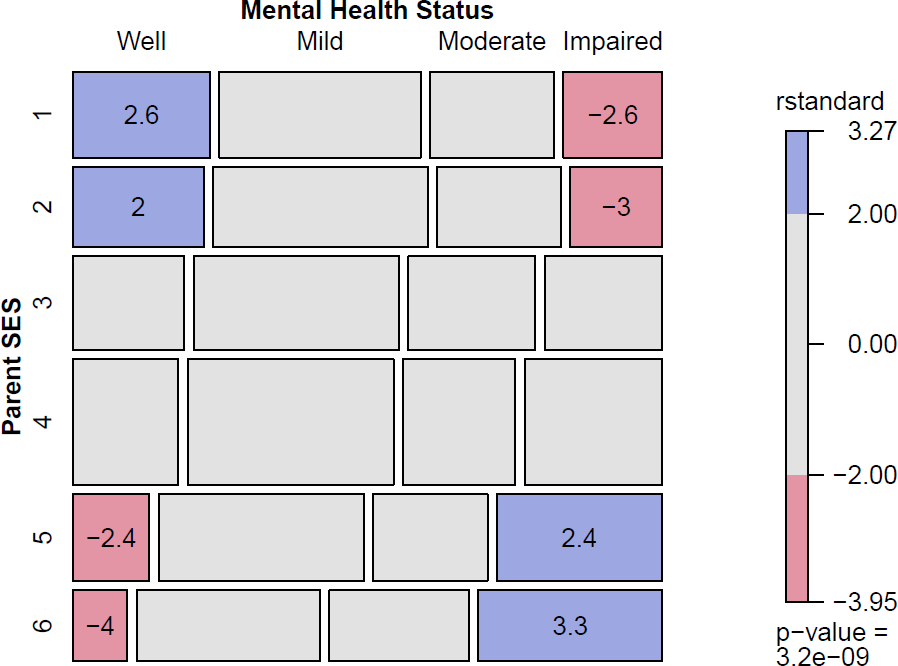
\includegraphics[width=.8\textwidth]{front/fig/mental-plot1} 
% \\
% 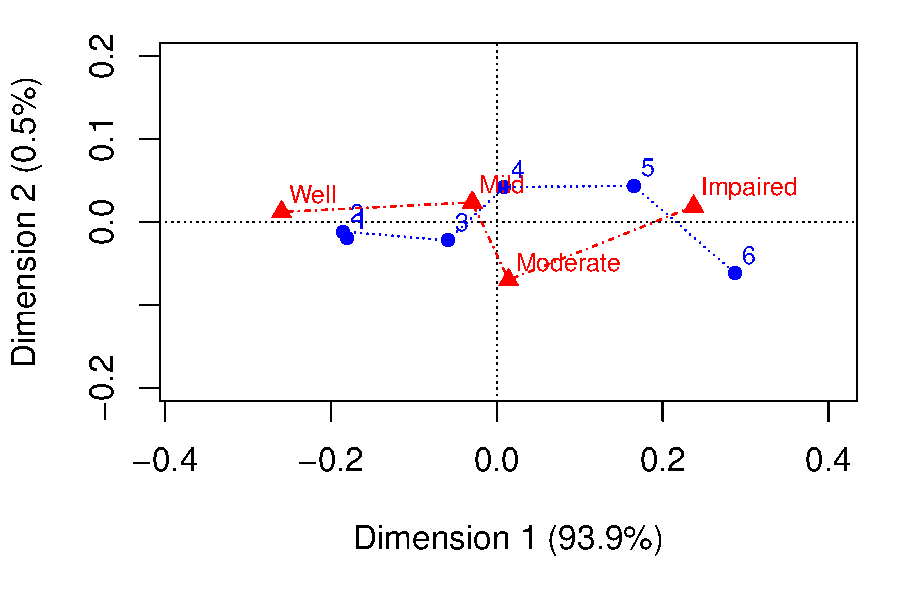
\includegraphics[width=.8\textwidth]{ch06/fig/ca-mental-plot}
}
%\end{titlepage}
\maketitle

%\begin{titlepage}
\title{%
%% simple cover pic for now
\Huge{Visualizing Categorical Data with }

\includegraphics[height=2ex, keepaspectratio]{front/fig/Rlogo}
% below-- use a graphic coverpage
%\input{front/covnew}
%\input{front/covpic}
}
\author{
	{\Large Michael Friendly} \\ York University
	\and
	{\Large David Meyer} \\ UAS Technikum Wien
%	\and
%	with contributions, \\ {\Large Achim Zeilleis} \\ Universit\"at Insbruck
}
\date{\today}
\vspace{1cm}
\titlepic{%
 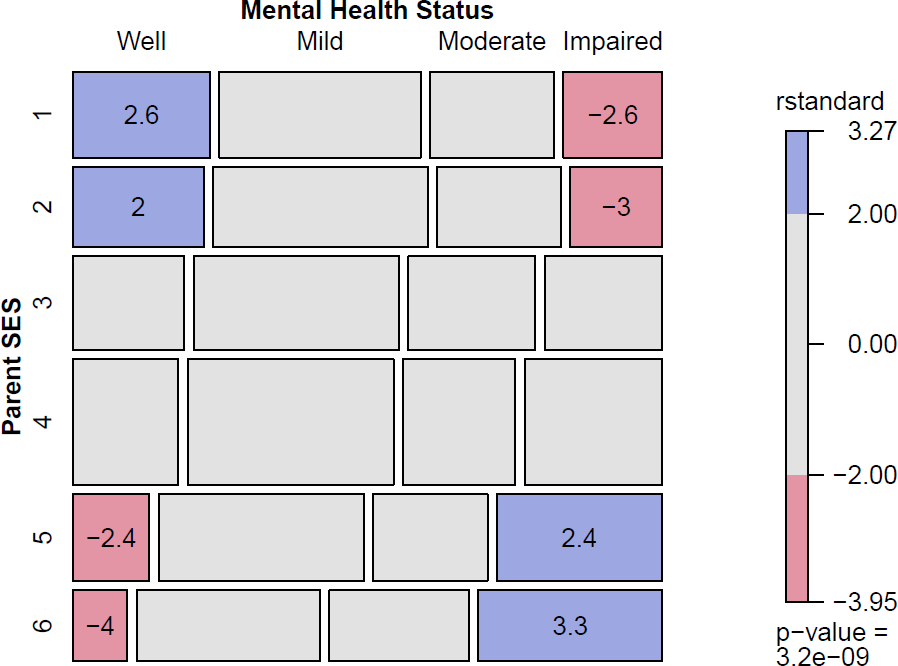
\includegraphics[width=.8\textwidth]{front/fig/mental-plot1} 
% \\
% 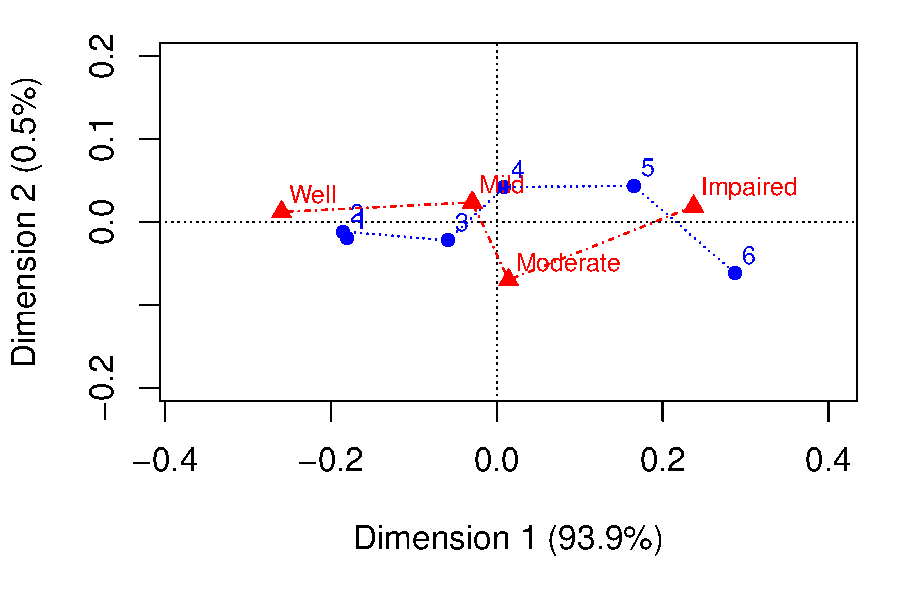
\includegraphics[width=.8\textwidth]{ch06/fig/ca-mental-plot}
}
%\end{titlepage}
\maketitle

%\begin{titlepage}
\title{%
%% simple cover pic for now
\Huge{Visualizing Categorical Data with }

\includegraphics[height=2ex, keepaspectratio]{front/fig/Rlogo}
% below-- use a graphic coverpage
%\input{front/covnew}
%\input{front/covpic}
}
\author{
	{\Large Michael Friendly} \\ York University
	\and
	{\Large David Meyer} \\ UAS Technikum Wien
%	\and
%	with contributions, \\ {\Large Achim Zeilleis} \\ Universit\"at Insbruck
}
\date{\today}
\vspace{1cm}
\titlepic{%
 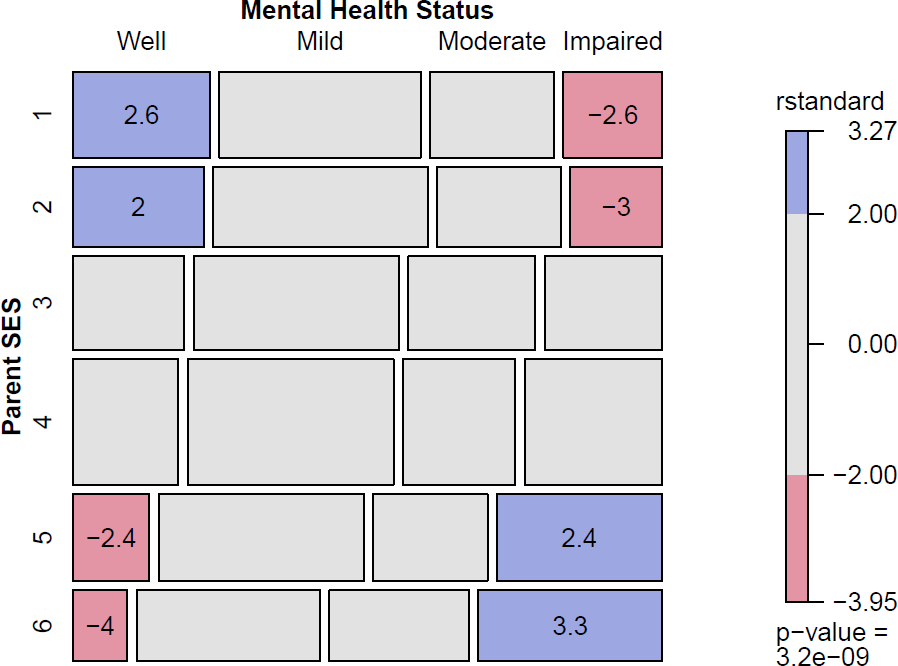
\includegraphics[width=.8\textwidth]{front/fig/mental-plot1} 
% \\
% 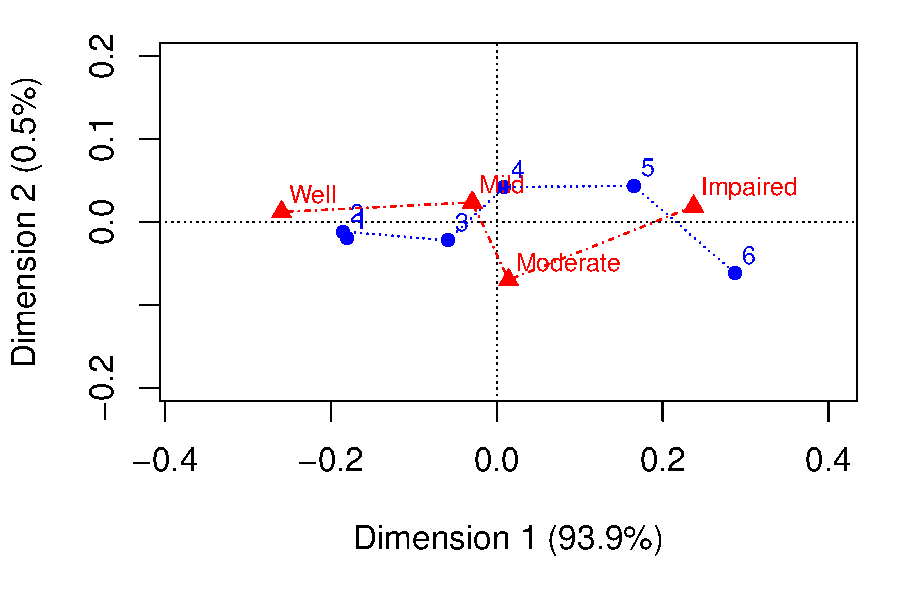
\includegraphics[width=.8\textwidth]{ch06/fig/ca-mental-plot}
}
%\end{titlepage}
\maketitle

\pagenumbering{roman}
%\addcontentsline{toc}{section}{Table of Contents}
{\renewcommand{\baselinestretch}{.8}\normalsize
\tableofcontents
}
%
%{\renewcommand{\baselinestretch}{.75}\normalsize
%\addcontentsline{toc}{section}{List of Tables}
%\listoftables
%}
%%
%{\renewcommand{\baselinestretch}{.75}\normalsize
%\addcontentsline{toc}{section}{List of Figures}
%\listoffigures
%}
%
%{\renewcommand{\baselinestretch}{.75}\normalsize
%\addcontentsline{toc}{section}{List of Outputs}
%\listof{Output}{List of Outputs}
%}
%
%\addtocontents{toc}{\protect\addcontentsline{toc}{section}{Table of Contents}}

%\chapter{Preface}
%\addcontentsline{toc}{chapter}{\numberline{}Preface}

\TODO{The preface has not yet been written.  This is just a stub.}

\section*{Audience}
% This book assumes basic understanding of statistical concepts at least at an
% intermediate undergraduate level including regression and analysis of variance
% (for example, at the level of \citet{Neter-etal:90,MendenhallSincich:2003}).
% 
% It is written to appeal to two audiences:
% \begin{itemize*}
%   \item Students and methodologists in the social and health sciences, epidemiology,
%     economics, business
% 	and (bio)statistics
% 	\item Substantive researchers in various disciplines wanting to be able to
% 	apply these methods to their own data
% \end{itemize*}
% 
% It is also assumed that the reader has at least basic knowledge of the \R language and
% environment, including interacting with the \R console (RGui for Windows, R.app for Mac OS X)
% or other graphical user interface (e.g., R Studio), using \R functions in packages,
% getting help for these from \R, etc.  One introductory chapter (\chref{ch:working}) is devoted
% to covering topics beyond such basic skills needed in the book.

\section*{Overview}

\section*{Acknowledgements}


%% ============ Main matter ================
\mainmatter
\pagenumbering{arabic}




\chapter{Introduction}\label{ch:intro}
%\begin{center}
 \rule[-4pt]{0.5pt}{4pt}\hrulefill\rule[-4pt]{0.5pt}{4pt}\\
 \begin{minipage}[c]{.33\linewidth}
  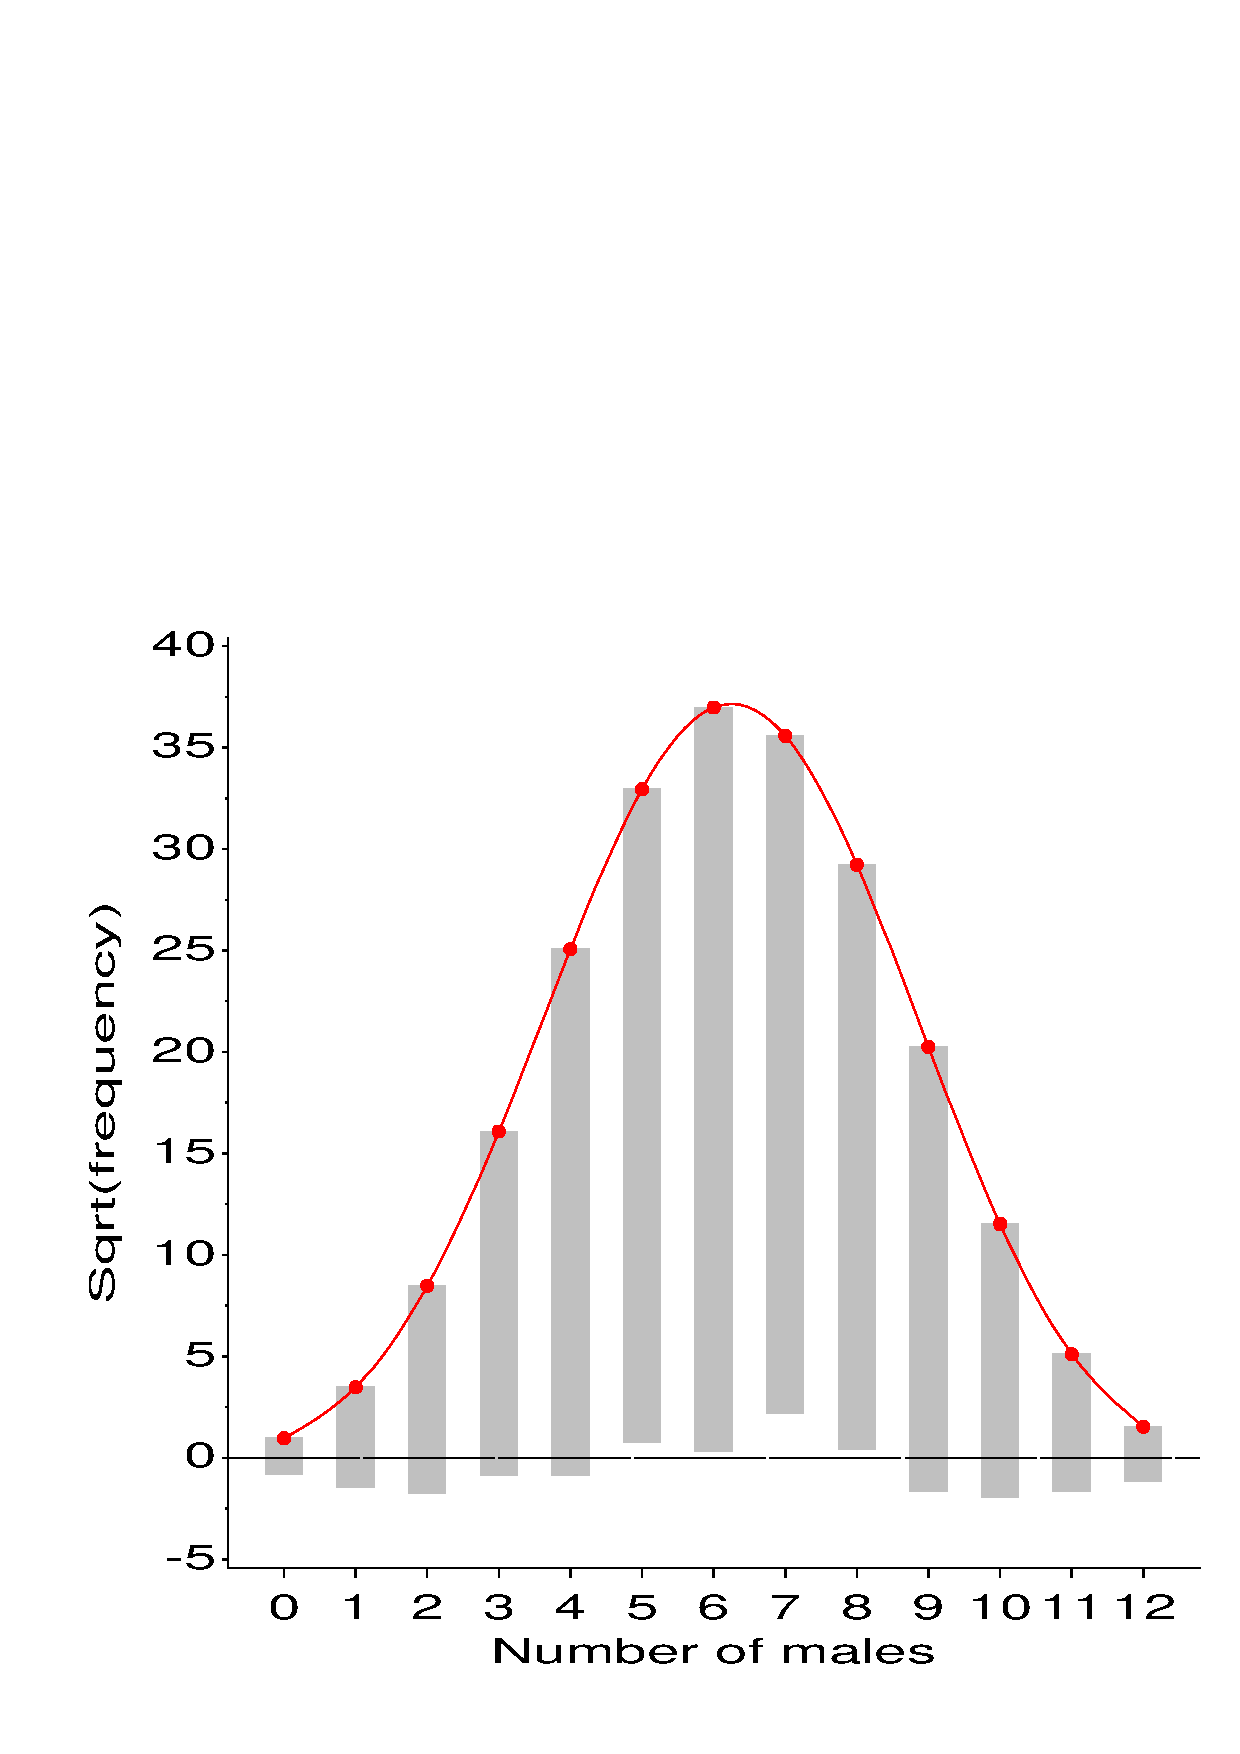
\includegraphics[width=1\linewidth]{saxony}\graphicsfile{ch2/fig/saxony.eps}{}
 \end{minipage}%
 \hfill
 \begin{minipage}[c]{.33\linewidth}
  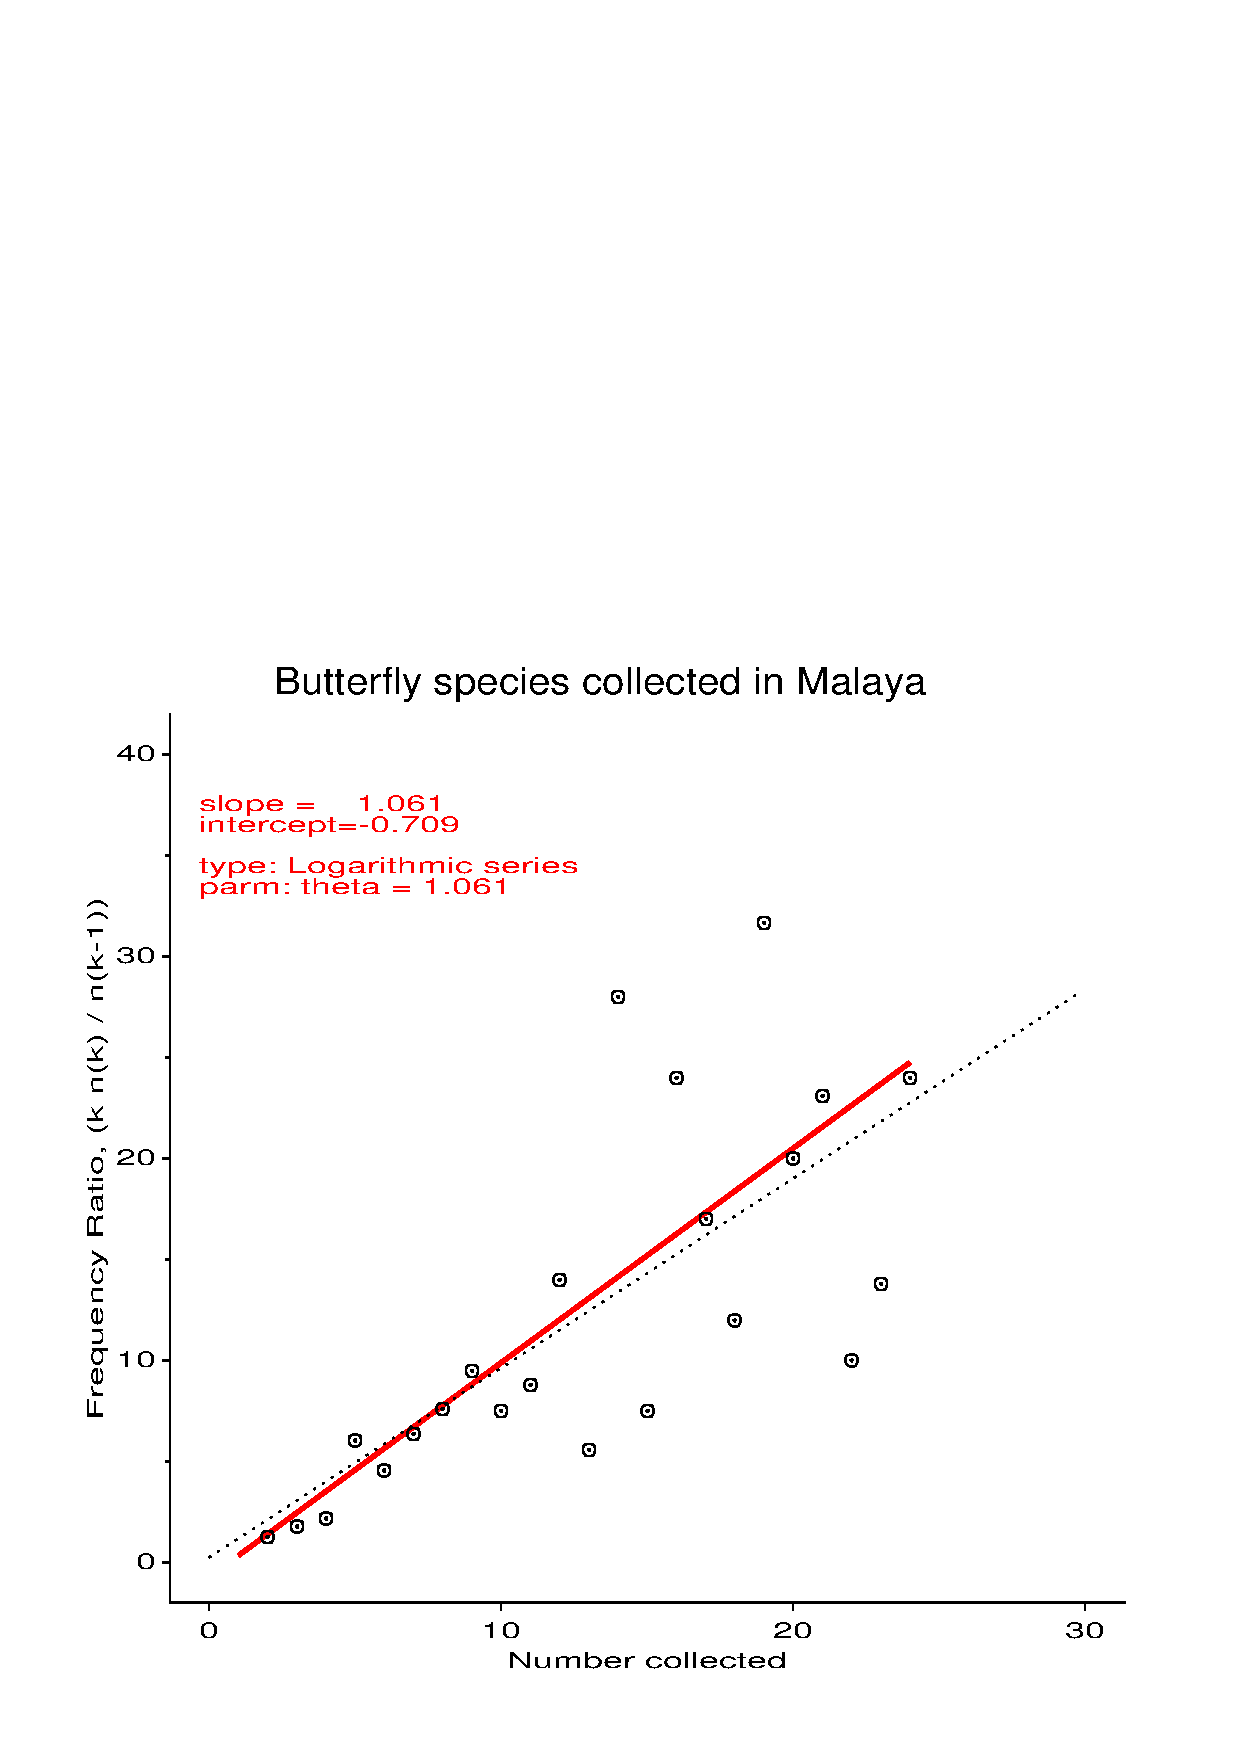
\includegraphics[width=1\linewidth]{orddemo3}\graphicsfile{ch2/fig/orddemo3.eps}{}
 \end{minipage}
 \hfill
 \begin{minipage}[c]{.33\linewidth}
  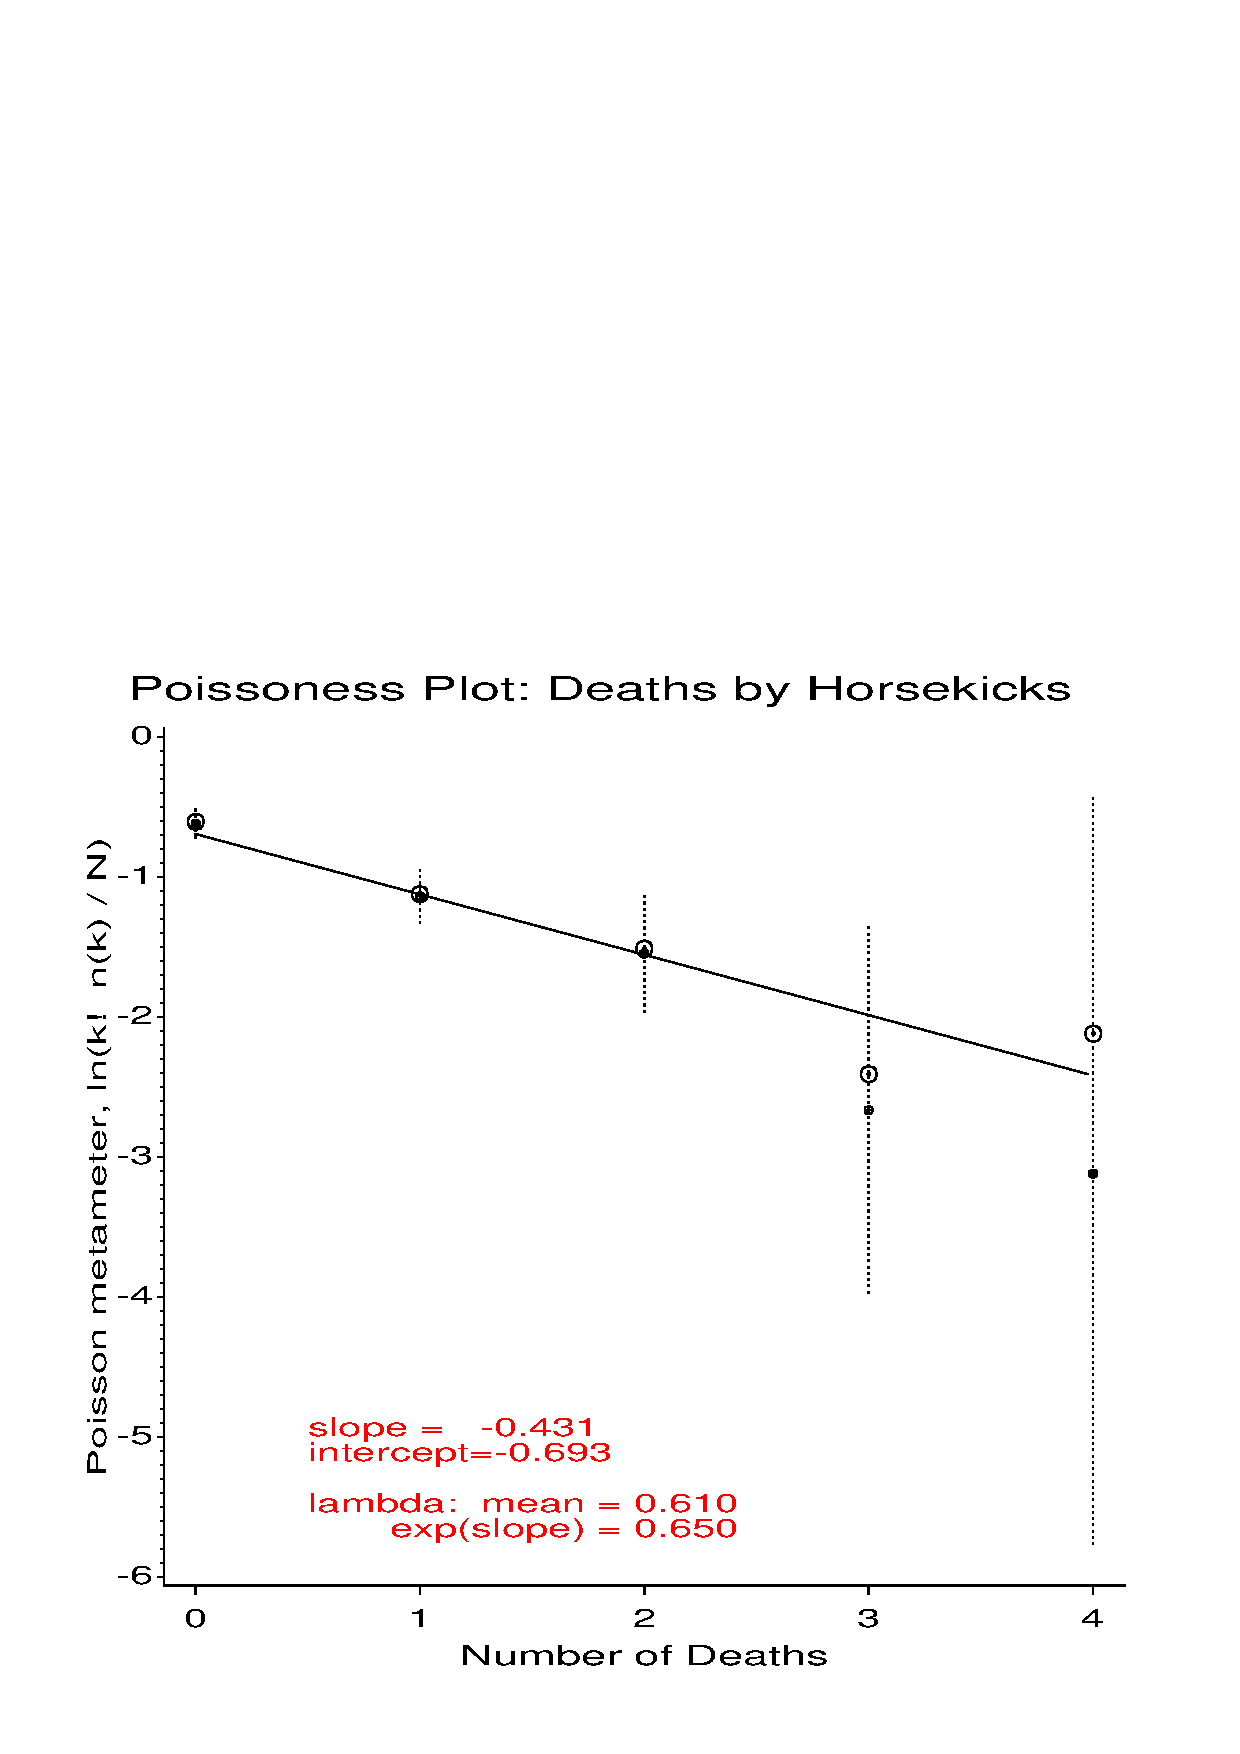
\includegraphics[width=1\linewidth]{poisdemo1}\graphicsfile{ch2/fig/poisdemo1.eps}{}
 \end{minipage}
\end{center}

		% visual table of contents

\chapterprelude{
Categorical data consists of variables whose values comprise a set
of discrete categories.
Such data require different statistical and graphical methods
than commonly used for quantitative data.
The focus of this book is on visualization techniques and graphical
methods designed to reveal patterns of relationships among
categorical variables. This chapter outlines the basic orientation
of the book and some key distinctions regarding the
analysis and visualization of
categorical data.
}
% \minitoc
% \clearpage


\section{Data visualization and categorical data: Overview}\label{sec:viscat}

\epigraph{Beauty is truth; truth, beauty. \\
  That is all ye know on Earth,
  all ye need to know.}{John Keats, \emph{Ode on a Grecian urn}}


``Data visualization'' can mean many things, from popular press
infographics, to maps of voter turnout or party choice.
Here we use this term in the narrower context of statistical
analysis.  As such, we refer to an approach to data analysis that focuses
on \emph{insightful} graphical display in the service of both
\emph{understanding} our data and \emph{communicating} our results to others.

We may display the raw data, some
summary statistics, or some indicators of the quality or adequacy
of a fitted model.  The word ``insightful'' suggests that the goal
is (hopefully) to reveal some aspects of the data which might not
be perceived, appreciated, or absorbed by other means.  
As in the quote from Keats, the overall
aims include both beauty and truth, though each of these are 
only as perceived by the beholder.

Methods for visualizing quantitative data have a long history
and are now widely used in both data analysis and in data presentation, and
in both popular and scientific media.
Graphical methods for categorical data,
however, have only a more recent history, and are consequently
not as widely used.  The goal of this book is to show concretely how
data visualization may be usefully applied to categorical data.

``Categorical'' data means different things in different
contexts.  We introduce the topic in \secref{sec:whatis}
with some examples illustrating
\begin{seriate}
\item types of categorical variables: binary, nominal, and ordinal,
\item data in case form vs.\ frequency form,
\item frequency data vs.\ count data,
\item univariate, bivariate, and multivariate data, and
\item the distinction between explanatory and response variables.
\end{seriate}

Statistical methods for the analysis of categorical data also fall into two
quite different categories, described and illustrated in \secref{sec:strategies}: 
\begin{seriate}
\item the simple randomization-based
methods typified by
the classical Pearson $\chi^2$, Fisher's exact test, and Cochran-Mantel-Haenszel
tests, and 
\item the model-based methods represented by
logistic regression, \loglin, and generalized linear models.
\end{seriate}
In this book, \chrange{ch:discrete}{ch:corresp}
are mostly related to the randomization-based methods; 
\chrange{ch:logistic}{ch:loglin}
illustrate the model-based methods.

In \secref{sec:methods} we describe some important similarities
and 
differences between categorical data and
quantitative data, and discuss the implications of these differences for
visualization techniques.
\secref{sec:vis} outlines a strategy of data analysis
focused on visualization.

In a few cases we show \R code or results as illustrations here,
but the fuller discussion of using \R for categorical data
analysis is postponed to \chref{ch:working}.


\section{What is categorical data?}\label{sec:whatis}

A \term{categorical variable} is one for which the possible measured
or assigned values
consist of a discrete set of categories, which may be \emph{ordered} or
\emph{unordered}.
Some typical examples are:
\begin{itemize*}
\item \var{Gender}, with categories ``Male'', ``Female''.
\item \var{Marital status}, with categories ``Never married'', ``Married'',
``Separated'', ``Divorced'', ``Widowed''.
\item \var{Fielding position} (in baseball), with categories
``Pitcher'', ``Catcher'', ``1st base'', ``2nd base'',  $\dots$, ``Left field''.
\item \var{Side effects} (in a pharmacological study), with categories
``None'', ``Skin rash'', ``Sleep disorder'', ``Anxiety'', $\dots$.
\item \var{Political attitude}, with categories ``Left'', ``Center'', ``Right''.
\item \var{Party preference} (in Canada), with categories ``NDP'', ``Liberal'', ``Conservative'', ``Green''.
\item \var{Treatment outcome}, with categories ``no improvement'', ``some
improvement'', or ``marked improvement''.
\item \var{Age}, with categories ``0-9'', ``10-19'', ``20-29'', ``30-39'', 
$\dots$ .
\item \var{Number of children}, with categories $0, 1, 2, \dots$ .
\end{itemize*}

As these examples suggest, categorical variables differ in the number of
categories: we often distinguish 
\term{binary variables} such as \var{Gender}
from those with more than two categories (called \term{polytomous variables}).
For example, \tabref{tab:berk220} gives data on 4526 applicants
to graduate departments at the University of California at Berkeley
in 1973, classified by two binary variables, gender and admission status.
\ixe{Berkeley admissions}
\begin{table}[htb]
\caption{Admissions to Berkeley graduate programs}
\label{tab:berk220}
 \begin{center}
\begin{tabular}{lrr|r}
\hline
  & Admitted & Rejected & Total  \\
\hline
 Males & 1198 & 1493 & 2691  \\
 Females & 557 & 1278 & 1835  \\
\hline
 Total & 1755 & 2771 & 4526  \\
\hline
\end{tabular}
\end{center}
\end{table}

Some categorical variables (\var{Political attitude}, \var{Treatment outcome})
may have ordered categories (and are called \term{ordinal}),
while other (\term{nominal}) variables like \var{Marital status}
have unordered categories.%
\footnote{An ordinal variable may be defined as one whose categories are
\emph{unambiguously} ordered along a \emph{single} underlying dimension.
Both marital status and fielding position may be weakly ordered, but
not on a single dimension, and not unambiguously.} 
For example, \tabref{tab:arthrit0} shows a $2 \times 2 \times 3$ table of 
ordered outcomes (``none'', ``some'' or ``marked'' improvement)
to an active treatment for rheumatoid
arthritis compared to a placebo for men and women.
\ixe{Arthritis treatment}
\begin{table}[tb]

\caption{Arthritis treatment data}\label{tab:arthrit0}
\begin{center}
\begin{tabular}{ll|rrr|r}
\hline
     &  & \multicolumn{3}{c|}{Improvement}            &  \\
\hline
   Treatment&  Sex    &None    &Some    &Marked  &  Total \\[1ex]
\hline
   Active   &  Female &      6 &      5 &     16 &     27 \\
            &  Male   &      7 &      2 &      5 &     14 \\ [0.5ex]
%\hline
   Placebo  &  Female &     19 &      7 &      6 &     32 \\
            &  Male   &     10 &      0 &      1 &     11 \\[1ex]
\hline
   Total    &         &     42 &     14 &     28 &     84 \\
\hline
\end{tabular}
\end{center}
\end{table}



Finally, such variables differ in the
fineness or level to which some underlying observation has been
categorized for a particular purpose.
From one point of view, \emph{all} data
may be considered categorical because the precision of measurement
is necessarily finite, or an inherently continuous variable may be recorded only to limited precision.   

But this view is not helpful for the applied
researcher because it neglects the phrase ``for a particular purpose''.
Age, for example, might be treated as a quantitative variable in a study of native language vocabulary, or as an ordered categorical variable 
with decade groups (0-10, 11-20, 20-30, $\dots$)
in terms of
the efficacy or side-effects of treatment for depression, or even as a
binary variable (``child'' vs.\  ``adult'') in an analysis of survival following an epidemic or natural disaster. In the analysis of
data using categorical methods, continuous variables are often recoded
into ordered categories with a small set of categories for some purpose.%
\footnote{
This may be wasteful of information available in the original
variable, and should be done for substantive reasons, not mere
convenience.  For example, some researchers unfamiliar with
regression methods often perform a ``median-split'' on 
quantitative predictors
so they can use ANOVA methods. Doing this precludes the possibility
of determining if those variables have non-linear relations with
the outcome.
}

\subsection{Case form vs.\ frequency form}\label{sec:case-freq}
In many circumstances, data is recorded on each individual or experimental
unit.  Data in this form is called case data,
or data in \term{case form}.
The data in \tabref{tab:arthrit0}, for example, were derived from
the individual data listed in the data set \data{Arthritis}
from the \Rpackage{vcd}.  The following lines show the first
five  of $N=84$ cases in the \data{Arthritis} data,
\begin{knitrout}
\definecolor{shadecolor}{rgb}{0.969, 0.969, 0.969}\color{fgcolor}\begin{kframe}
\begin{alltt}
\hlkwd{data}\hlstd{(}\hlstr{"Arthritis"}\hlstd{,} \hlkwc{package}\hlstd{=}\hlstr{"vcd"}\hlstd{)}
\hlkwd{head}\hlstd{(Arthritis,} \hlnum{5}\hlstd{)}
\end{alltt}
\begin{verbatim}
##   ID Treatment  Sex Age Improved
## 1 57   Treated Male  27     Some
## 2 46   Treated Male  29     None
## 3 77   Treated Male  30     None
## 4 17   Treated Male  32   Marked
## 5 36   Treated Male  46   Marked
\end{verbatim}
\end{kframe}
\end{knitrout}


Whether or not the data variables, and the questions we ask, call for
categorical or quantitative data analysis, 
when the data are in case form,
we can always trace
any observation back to its individual identifier or data record
(for example, if the case with \code{ID==57} turns out to be unusual
or noteworthy).

Data in \term{frequency form} 
has already been tabulated, by counting over the categories of the
table variables. The same data shown as a table in 
\tabref{tab:arthrit0} appear in frequency form as shown below.
\begin{knitrout}
\definecolor{shadecolor}{rgb}{0.969, 0.969, 0.969}\color{fgcolor}\begin{kframe}
\begin{alltt}
\hlkwd{as.data.frame}\hlstd{(}\hlkwd{xtabs}\hlstd{(}\hlopt{~}\hlstd{Treatment}\hlopt{+}\hlstd{Sex}\hlopt{+}\hlstd{Improved,} \hlkwc{data}\hlstd{=Arthritis))}
\end{alltt}
\begin{verbatim}
##    Treatment    Sex Improved Freq
## 1    Placebo Female     None   19
## 2    Treated Female     None    6
## 3    Placebo   Male     None   10
## 4    Treated   Male     None    7
## 5    Placebo Female     Some    7
## 6    Treated Female     Some    5
## 7    Placebo   Male     Some    0
## 8    Treated   Male     Some    2
## 9    Placebo Female   Marked    6
## 10   Treated Female   Marked   16
## 11   Placebo   Male   Marked    1
## 12   Treated   Male   Marked    5
\end{verbatim}
\end{kframe}
\end{knitrout}


Data in frequency form may be analyzed by methods
for quantitative data if there is a quantitative response variable
(weighting each group by the cell frequency, with a \code{weight}
variable).  
Otherwise, such data are generally
best analyzed by methods for categorical data, where
statistical models are often expressed as models for the
frequency variable, in the form of an \R formula
like \verb|Freq ~ .|.

In any case, an observation in a data set in
frequency form refers
to all cases in the cell collectively, and these cannot be identified individually.
Data in case form can always be reduced to frequency form,
but the reverse is rarely possible. In \chref{ch:working},
we identify a third format, \term{table form}, which is the
\R representation of a table like \tabref{tab:arthrit0}.

\subsection{Frequency data vs.\ count data}\label{sec:freq-count}
In many cases the observations represent the classifications of events or variables are 
recorded from \emph{operationally independent} experimental units or individuals, typically
a sample from some population.  The tabulated data may be called
\term{frequency data}.  The data in \tabref{tab:berk220} and \tabref{tab:arthrit0}
are both examples of frequency data because each observation tabulated
comes from a different person.

However, if several events or variables are observed for the same units or individuals, those events are not
operationally independent, and it is useful to use the term 
\term{count data} in this situation.  These terms (following
\citet{Lindsey:95}) are by no means standard, but
the distinction is often important, particularly in statistical
models for categorical data.  

For example, in a tabulation of the number of male
children within families (\tabref{tab:saxdata}, described in
\secref{sec:uni-multi} below), 
the number of male children in a given family would be a \emph{count} variable,
taking values $0, 1, 2, \dots$.  The number of independent families with
a given number of male children is a \emph{frequency} variable.
Count data also arise when we tabulate a sequence of events over time
or under different circumstances in a number of individuals.

\ixe{Families in Saxony}
\begin{table}[htb]
 \caption{Number of Males in 6115 Saxony Families of Size 12}\label{tab:saxdata}
 \begin{center}
 \begin{tabular}{lrrrrrrrrrrrrr}
  \hline
  Males & 0 & 1 & 2 & 3 & 4 & 5 & 6 & 7 & 8 & 9 & 10 & 11 & 12 \\ 
  Families & ~~~3 & ~~24 & ~104 & ~286 & ~670 & 1033 & 1343 & 1112 & ~829 & ~478 & 181 & ~~45 & ~~~7 \\ 
  \hline
 \end{tabular}
 \end{center}
\end{table}


\subsection{Univariate, bivariate, and multivariate data}\label{sec:uni-multi}
Another distinction concerns the number of variables: one, two or
(potentially) many shown in a data set or table, or used in some
analysis.
\tabref{tab:berk220} is an example of a bivariate (two-way) \ctab
and \tabref{tab:arthrit0} classifies the observations by three variables.
Yet, we will see later
that the Berkeley admissions data also recorded
the department to which potential students applied (giving a three-way
table), and in the arthritis data, the age of subjects was also
recorded.

Any \ctab (in frequency or table form) therefore records the \emph{marginal totals}, summed over all
variables not represented in the table.
For data in case form, this means simply ignoring (or not recording)
one or more variables;  the ``observations'' remain the same.
Data in frequency form, however, result in smaller tables when
any variable is ignored;  the ``observations'' are the cells of
the \ctab. For example, in the \data{Arthritis} data, ignoring \var{Sex}
gives the smaller $2 \times 3$ table for \var{Treatment} and \var{Improved}.
\begin{knitrout}
\definecolor{shadecolor}{rgb}{0.969, 0.969, 0.969}\color{fgcolor}\begin{kframe}
\begin{alltt}
\hlkwd{as.data.frame}\hlstd{(}\hlkwd{xtabs}\hlstd{(}\hlopt{~}\hlstd{Treatment} \hlopt{+} \hlstd{Improved,} \hlkwc{data}\hlstd{=Arthritis))}
\end{alltt}
\begin{verbatim}
##   Treatment Improved Freq
## 1   Placebo     None   29
## 2   Treated     None   13
## 3   Placebo     Some    7
## 4   Treated     Some    7
## 5   Placebo   Marked    7
## 6   Treated   Marked   21
\end{verbatim}
\end{kframe}
\end{knitrout}



In the limiting case, only one table variable may be recorded or
available, giving the categorical equivalent of univariate data.
For example, \tabref{tab:saxdata} gives data on the distribution
of the number of male children in families with 12 children
(discussed further in \exref{ex:saxony1}).
These data were part of a large tabulation of the sex distribution
of families in Saxony in the 19$^{th}$ century, but the data in \tabref{tab:saxdata}
have only one discrete classification variable, number of males.
Without further information, the only statistical questions concern
the form of the distribution.
We discuss methods for fitting and graphing such discrete distributions
in \chref{ch:discrete}.
The remaining chapters relate to bivariate and multivariate data.
\ixe{Families in Saxony}


\subsection{Explanatory vs.\ Response variables}\label{sec:exp-resp}
\ix{variable!response \~|(}
Most statistical models make a distinction between \term{response variables}
(or \emph{dependent}, or \emph{criterion} variables)
and
\term{explanatory variables}
(or \emph{independent}, or \emph{predictor} variables).

In the standard (classical) linear models for regression and analysis of variance
(ANOVA), for instance, we treat one (or more) variables as responses,
to be explained by the other, explanatory variables.
The explanatory variables may be quantitative or categorical
(e.g., factors in \R). 
This affects only the details of how the model is specified
or how coefficients are interpreted for
\func{lm} or \func{glm}.  In these classical models,
the response variable (``treatment outcome'', for example), must be
considered quantitative,  and the model attempts to describe how the
\emph{mean} of the distribution of responses changes with the values
or levels of the explanatory variables, such as age or gender.

However, when the response variable is categorical, however, the standard linear
models do not apply, because they assume a normal (Gaussian) distribution
for the model residuals.  For example, in \tabref{tab:arthrit0} 
the response variable
is \var{Improvement}, and even if numerical scores were assigned
to the categories ``none'', ``some'', ``marked'', it may be unlikely
that the assumptions of the classical linear models could be met.

Hence, a categorical \emph{response} variable generally requires analysis
using methods for categorical data, but categorical \emph{explanatory} variables
may be readily handled by either method.

The distinction between response and explanatory variables also
becomes important in the use of \loglin models for frequency tables
(described in \chref{ch:loglin}), where models can be specified
in a simpler way (as equivalent logit models) by focusing on the response
variable.
\ix{variable!response \~|)}


\section{Strategies for categorical data analysis}\label{sec:strategies}

Methods of analysis for categorical data can be classified into two
broad categories:
those concerned with hypothesis testing \emph{per se}, and those concerned with model building.

\subsection{Hypothesis testing approaches}\label{sec:strategies-hyp}
In many studies, the questions of substantive interest translate readily
into questions concerning hypotheses about \term{association} between variables, a more general idea than that of correlation 
(\emph{linear} association) for quantitative variables.
If a non-zero association exists, we may wish to characterize the
strength of the association numerically and understand the pattern or
nature of the association.

For example, in \tabref{tab:berk220}, a main question is:
``Is there evidence of gender-bias in admission to graduate school?''
Another way to frame this: ``Are males more likely to be admitted?''
These questions can
be expressed in terms of an association between gender and
admission status in a $2 \times 2$ \ctab\
of applicants classified by these two variables.
If there is evidence for an association, we can assess its strength by a variety of
measures, including the difference in proportions admitted for men
and women or the ratio of the odds of admission for men compared to
women, as described in \secref{sec:twoway-twobytwo}.

Similarly, in \tabref{tab:arthrit0}, questions about the efficacy of the
treatment for rheumatoid arthritis can be answered in terms of
hypotheses about the associations among the table variables:
\var{Treatment}, \var{Sex}, and the \var{Improvement} categories.
Although the main concern might be focused on the overall association between
Treatment and Improvement, one would also wish to know if this association
is the same for men and women.  
A \term{stratified analysis} (\secref{sec:twoway-strat}) controls for the effects of background
variables like Sex, and tests for \term{homogeneity of association}
help determine if these associations are equal.

Questions involving tests of such hypotheses are answered most easily
using a large variety of specific statistical tests, often based on
randomization arguments.
These include the familiar Pearson chi-square test for two-way tables,
the Cochran-Mantel-Haenszel test statistics, Fisher's exact test, and a wide range of measures of strength of association.
These tests make minimal assumptions, principally requiring that subjects
or experimental units have been randomly assigned to the categories of
experimental factors.  The hypothesis testing approach is illustrated
in \chref{ch:twoway}--\ref{ch:corresp}, though the emphasis is on graphical
methods which help to understand the nature of association between
variables.

\begin{Example}[haireye0]{Hair color and eye color}
%\begin{table}[htb]

\caption{Hair-color eye-color data}\label{tab:hairdat}
\begin{center}
\begin{tabular}{|lrrrr|r|}
\hline
        & \multicolumn{4}{c|}{Hair Color}        & \\
Eye     &         &         &         &         &       \\
Color   &  Black  &  Brown  &    Red  &  Blond  & Total \\[2ex] \hline
Green   &      5  &     29  &     14  &     16  &    64 \\
Hazel   &     15  &     54  &     14  &     10  &    93 \\
Blue    &     20  &     84  &     17  &     94  &   215 \\
Brown   &     68  &    119  &     26  &      7  &   220 \\[1ex] \hline
Total   &    108  &    286  &     71  &    127  &   592 \\ \hline
\end{tabular}
\end{center}
\end{table}


%\tabref{tab:hairdat} 
The data \data{HairEye} below
records data on the the relationship between hair color and eye color
in a sample of nearly 600 students.
\begin{knitrout}
\definecolor{shadecolor}{rgb}{0.969, 0.969, 0.969}\color{fgcolor}\begin{kframe}
\begin{alltt}
\hlkwd{library}\hlstd{(vcd)}
\hlstd{(HairEye} \hlkwb{<-} \hlkwd{margin.table}\hlstd{(HairEyeColor,} \hlkwd{c}\hlstd{(}\hlnum{1}\hlstd{,} \hlnum{2}\hlstd{)))}
\end{alltt}
\begin{verbatim}
##        Eye
## Hair    Brown Blue Hazel Green
##   Black    68   20    15     5
##   Brown   119   84    54    29
##   Red      26   17    14    14
##   Blond     7   94    10    16
\end{verbatim}
\end{kframe}
\end{knitrout}


The standard analysis (with \func{chisq.test} or \func{assocstats})
gives a 
Pearson \(\chi^2\) of 138.3 with nine degrees of freedom,
indicating substantial departure from independence.  Among the measures of
strength of association, the \term{phi coefficient},
$\phi = \sqrt{\chi^2 / N} = 0.483$, indicates a substantial relationship
between hair and eye color.

\begin{knitrout}
\definecolor{shadecolor}{rgb}{0.969, 0.969, 0.969}\color{fgcolor}\begin{kframe}
\begin{alltt}
\hlkwd{assocstats}\hlstd{(HairEye)}
\end{alltt}
\begin{verbatim}
##                     X^2 df P(> X^2)
## Likelihood Ratio 146.44  9        0
## Pearson          138.29  9        0
## 
## Phi-Coefficient   : 0.483 
## Contingency Coeff.: 0.435 
## Cramer's V        : 0.279
\end{verbatim}
\end{kframe}
\end{knitrout}

The further (and perhaps more interesting question) is how do we
understand the \emph{nature} of this association between hair
and eye color?
Two graphical methods related to the hypothesis testing approach
are shown in \figref{fig:haireye02}.

\begin{knitrout}
\definecolor{shadecolor}{rgb}{0.969, 0.969, 0.969}\color{fgcolor}\begin{figure}[htbp]


\centerline{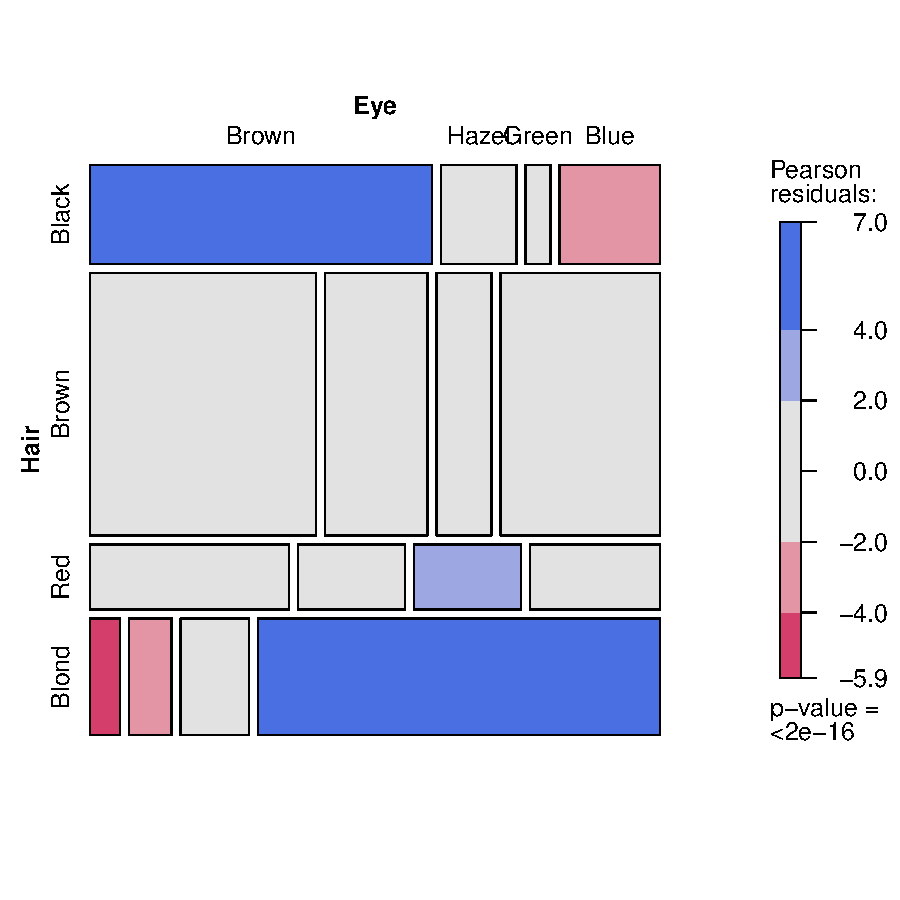
\includegraphics[width=.49\textwidth]{ch01/fig/haireye021} 
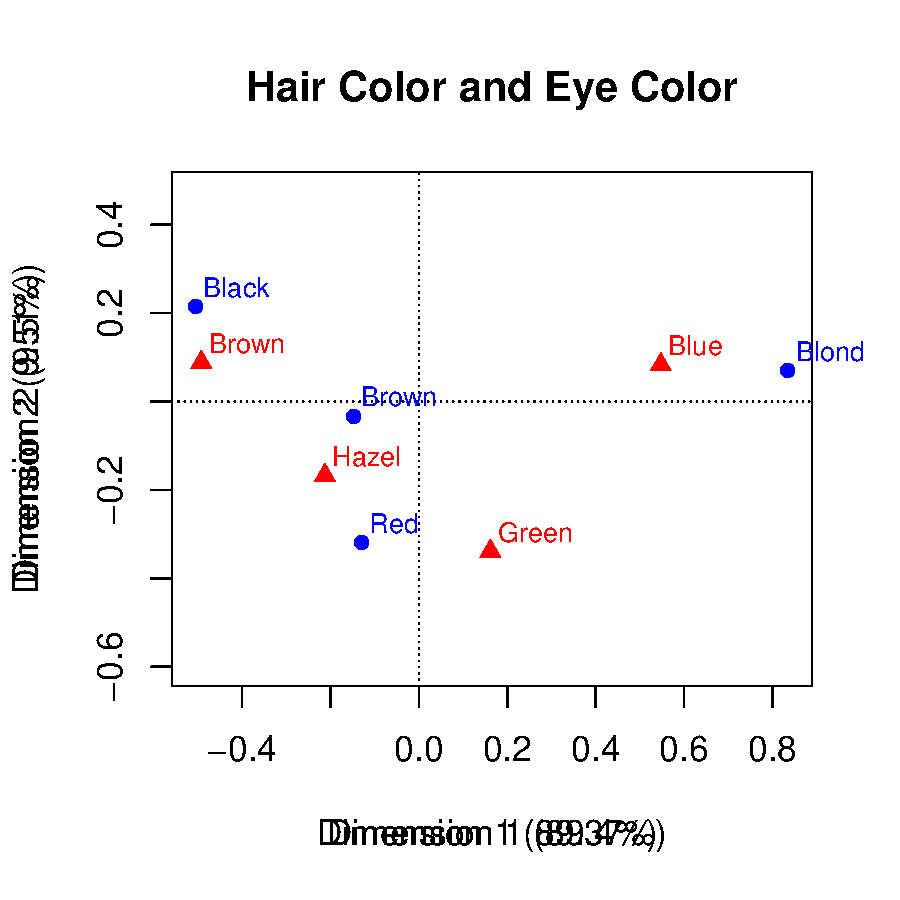
\includegraphics[width=.49\textwidth]{ch01/fig/haireye022} }

\caption[Graphical displays for the hair color and eye color data]{Graphical displays for the hair color and eye color data. Left: mosaic display; right: correspondence analysis plot\label{fig:haireye02}}
\end{figure}


\end{knitrout}

The left panel of \figref{fig:haireye02} is a \term{mosaic display}
(\chref{ch:mosaic}), constructed so that the size of each rectangle
is proportional to the observed cell frequency. The shading
reflects the cell contribution to the \(\chi^2\) statistic---shades of blue
when the observed frequency is substantially greater than the 
expected frequency under independence, shades of red when the observed frequency
is substantially less, as shown in the legend.

The right panel of this figure shows the results of 
a \ca (\chref{ch:corresp}), where the deviations of the hair color and eye
color points from the origin accounts for as much of the \(\chi^2\)
as possible in two dimensions.

We observe that both the hair colors and the eye colors
are ordered from dark to light in the mosaic display and along
Dimension 1 in the \ca plot.  The deviations between observed
and expected frequencies have an opposite-corner pattern in the
mosaic display, except for the combination of red hair and green
eyes, which also stand out as the largest values on Dimension 2
in the \CA plot.
Displays such as these provide a means to understand \emph{how}
the variables are related.
\end{Example}

\subsection{Model building approaches}
Model-based methods provide tests of equivalent
hypotheses about associations, but 
offer additional advantages (at the cost of additional assumptions)
not provided by the simpler hypotheses-testing approaches.
Among these advantages, model-based methods provide estimates,
standard errors and confidence intervals for parameters, and the
ability to obtain predicted (fitted) values with associated measures
of precision.

We illustrate this approach here for a dichotomous response variable,
where it is often convenient to
construct a model relating a function of the probability, $\pi$,
of one event to a linear combination of the explanatory variables.
Logistic regression uses the \term{logit function},
\begin{equation*}
 \logit ( \pi ) \equiv \log_e \left( \frac { \pi } {1 - \pi} \right)
\end{equation*}
which may be interpreted as the \term{log odds} of the given event.
A linear logistic model 
can then be expressed as
\begin{equation*}
 \logit ( \pi ) = \beta_0 + \beta_1 x_1 + \beta_2 x_2 + \dots
\end{equation*}

Statistical inferences from model-based methods provide tests of
hypotheses for the effects of the predictors, $x_1, $x_2, \dots$,
but they also provide estimates of parameters in the model,
$\beta_1, \beta_2, \dots$ and associated confidence intervals.
Standard modeling tools allow us to graphically display the 
fitted response surface (with confidence or prediction intervals)
and even to extrapolate these predictions beyond the given data.
A particular advantage of the logit represent ion
in the logistic regression model is that estimates of odds ratios
(\secref{sec:twoway-odds})
may be obtained directly from the parameter estimates.

\begin{Example}[nasa0]{Space shuttle disaster}
\ixd{Space shuttle disaster|(}
To illustrate the model-based approach,
the graph in \figref{fig:spaceshuttle0} is based on
a logistic regression model predicting the probability of a
failure in one of the O-ring seals used in the 24 NASA space shuttles
prior to the disastrous launch of the 
\emph{Challenger} in January, 1986.  The explanatory variable is the ambient temperature at the time of the flight.
The sad story behind these data, and the lessons to be learned for
graphical data display are related in \exref{ex:nasa}.

\begin{knitrout}
\definecolor{shadecolor}{rgb}{0.969, 0.969, 0.969}\color{fgcolor}\begin{figure}[htbp]


\centerline{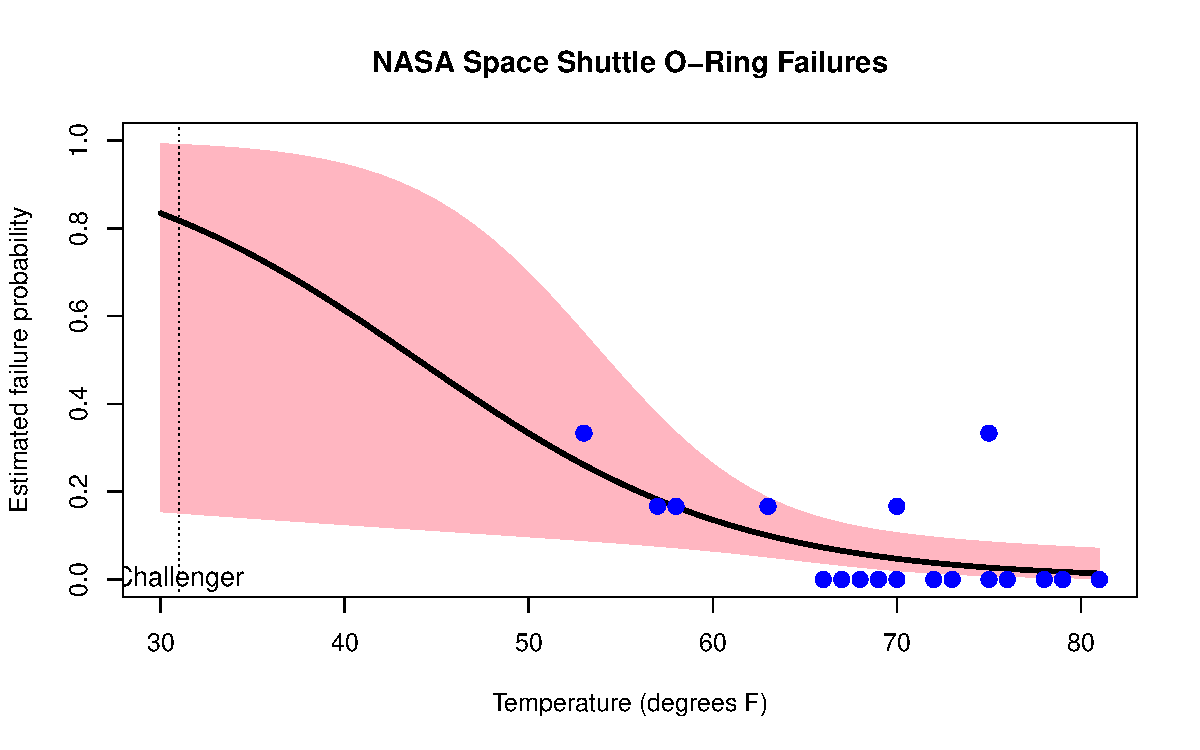
\includegraphics[width=.7\textwidth]{ch01/fig/spaceshuttle0} }

\caption[Space shuttle O-ring failure, observed and predicted probabilities]{Space shuttle O-ring failure, observed and predicted probabilities. The dotted vertical line at \degree{31} shows the prediction for the launch of the \emph{Challenger}.\label{fig:spaceshuttle0}}
\end{figure}


\end{knitrout}


Here, we simply note that the fitted model, shown by the solid line in
\figref{fig:spaceshuttle0}, corresponds to the prediction equation
(with standard errors shown in parentheses),
\begin{equation*}
 \logit ( \mbox{Failure} ) =  \cwe{5.09}{3.06} - \cwe{0.116}{0.047} \mbox{ Temperature} 
 \end{equation*}%
A hypothesis test that failure probability is unassociated with temperature
is equivalent to the test that the coefficient for temperature in this
model equals 0; this test has a $p$-value of 0.014, convincing evidence
for rejection.

The parameter estimate for temperature, $-0.116$, however, gives more information.  Each \degree{1} increase in temperature decreases the log odds
of failure by 0.116, with 95\% confidence interval ($-0.208$, $-0.0235$).  The equivalent odds ratio is $\exp(-0.116) = 0.891$ (0.812--0.977).
Equivalently, a \degree{10} \emph{decrease} in temperature corresponds to
an odds ratio of a failure of 
$\exp(10 \times 0.116) = 3.18$, more than tripling the odds of a failure.

When the \emph{Challenger} was launched, the temperature was only \degree{31}.
The shaded region in \figref{fig:spaceshuttle0} show 95\% prediction intervals
for failure probability.  All previous shuttles (shown by the points
in the figure) had been launched at much warmer temperatures, so the
prediction interval (the dashed vertical line)
at \degree{31} represents a considerable extrapolation
beyond the available data.  Nonetheless, the model building approach
does provide such predictions along with measures of their uncertainty.
\figref{fig:spaceshuttle0} is a graph
that might have saved lives.

\ixd{Space shuttle disaster|)}
\end{Example}

\TODO{Perhaps replace this example with a similar one for the \code{Donner} data}

\section{Graphical methods for categorical data}\label{sec:methods}

\epigraph{You can see a lot, just by looking}{Yogi Berra}

The graphical methods for categorical data described in this book
are in some cases straightforward adaptations of more familiar
visualization techniques developed for quantitative data.
Graphical principles and strategies, and the relations between
the visualization approach and traditional statistical methods
are described in a number of sources, including
\citet{Chambers-etal:83},
\citet{Cleveland:VisData} and several influential books by Tufte
\citep{Tufte:83,Tufte:90,Tufte:97,Tufte:2006}.

The fundamental ideas of statistical graphics as a comprehensive system
of visual signs and symbols with a grammar and semantics was first proposed
in Jacques Bertin's \emph{Semiology of Graphics} \citeyearpar{Bertin:83}, 
These ideas were later extended to a computational theory
in Wilkinson's \emph{Grammar of Graphics} \citeyearpar{Wilkinson:2005},
and implemented in \R in Hadley Wickham's \Rpackage{ggplot2}
\citep{Wickham:2009:ggplot2,ggplot2}.

Another perspective on visual data display is presented in \secref{sec:intro-goals}.
However, the discrete nature of categorical data implies that
some familiar graphic methods need to be adapted, while in other
cases we require a new graphic metaphor for data display.
These issues are illustrated in \secref{sec:intro-catdata}.

\subsection{Goals and design principles for visual data display}\label{sec:intro-goals}

Designing good graphics is surely an art, but as surely, it is
one that ought to be informed by science.
In constructing a graph, quantitative and qualitative information is
encoded by visual features, such as position, size, texture, symbols
and color. This translation is reversed when a person studies a
graph. The representation of numerical magnitude and categorical
grouping, and the apperception of patterns and their \emph{meaning} must be extracted from the visual display.  

There are many views of graphs, of graphical perception, and of
the roles of data visualization in discovering and communicating
information.
On the one hand, one may regard a graphical display as a \emph{stimulus}---
a package of information to be conveyed to an idealized observer.
From this perspective certain questions are of interest:  which
form or graphic aspect promotes greater accuracy or speed of judgment
(for a particular task or question)?  What aspects lead to greatest
memorability or impact? 
Cleveland \citep{ClevelandMcGill:84b,ClevelandMcGill:85,Cleveland:93:JCGS},
Spence and Lewandowsky 
\citep{LewandowskySpence:89,Spence:90,SpenceLewandowsky:90} have made important contributions to our understanding of
these aspects of graphical display.

An alternative view regards a graphical display as an act
of \emph{communication}---like a narrative, or even a poetic text or work of art. 
This perspective places the greatest emphasis on the desired
communication goal, and judges the effectiveness of a graphical
display in how well that goal is achieved \citep{FriendlyKwan:2011}.
\citet{Kosslyn:85,Kosslyn:89} and \citet{Tufte:83,Tufte:90,Tufte:97}
have articulated this perspective most clearly.

In this view,
an effective graphical display, like good writing, requires an
understanding of its \emph{purpose}---what aspects of the data are to be
communicated to the viewer.  In writing we communicate most
effectively when we know our audience and tailor the message
appropriately. So too, we may construct a graph in different ways to:
\begin{seriate}
  \item use ourselves, 
  \item present at a conference or meeting of our colleagues, 
  \item publish in a research report, or
  \item communicate to a general audience
\end{seriate}
(\citet[Ch. 1]{Friendly:91}, \citet{FriendlyKwan:2011}).
\figref{fig:presentation-exploration} illustrates a basic contrast between graphs
for presentation purposes, designed to appeal persuasively to a large audience
(one-to-many)
and the use of perhaps many graphs we might make for ourselves for 
exploratory data analysis (many-to-one).
% \citep{Unwin:99}.

\begin{figure}[htb]
\centering
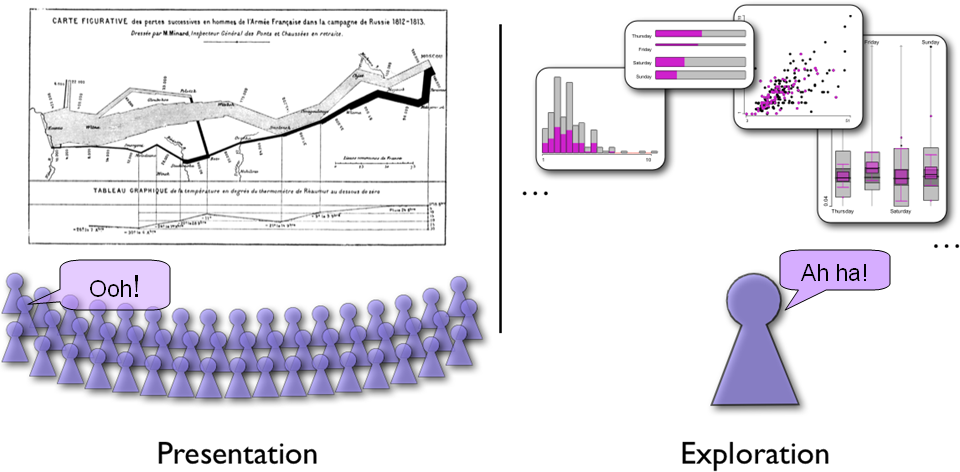
\includegraphics[width=.8\textwidth]{ch01/fig/presentation-exploration2}
\caption[Different communication purposes require different graphs]{Different communication purposes require different graphs. For presentations, a single, carefully crafted graph may appeal best to a large audience; for exploratory analysis, many related images from different perspectives for a narrow audience (often you!). \emph{Source}: Adapted from a blog entry by Martin Theus, \url{http://www.theusrus.de/blog/presentation-vs-exploration/}.}\label{fig:presentation-exploration}
\end{figure}

\figref{fig:datadisp}
shows one organization of visualization methods in terms
of the \emph{primary} use or intended communication goal,
the functional \emph{presentation goal}, and suggested corresponding
\emph{design principles}.
\begin{figure}[htbp]
  \centering 
  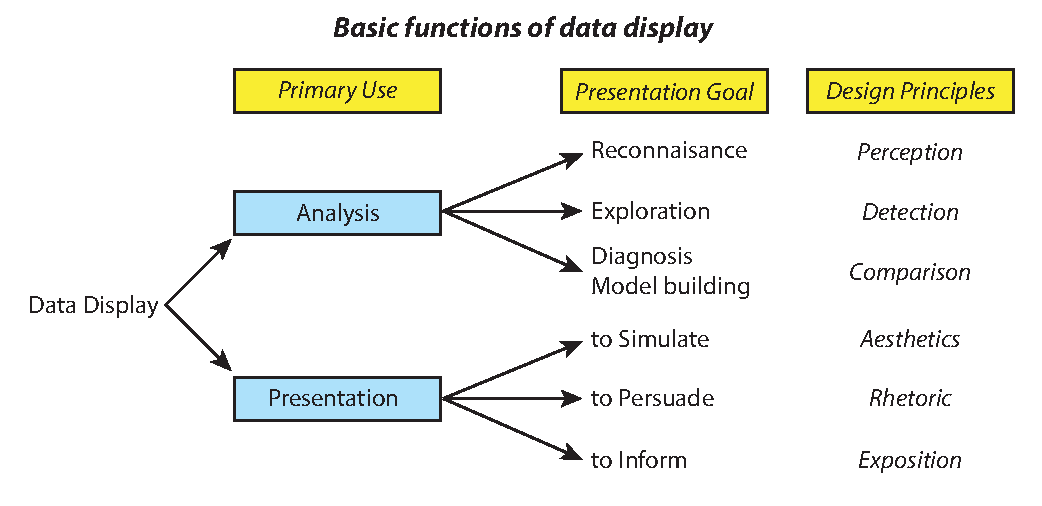
\includegraphics[width=\textwidth]{ch01/fig/datadisp}
  \caption[Basic functions of data display]{A taxonomy of the basic functions of data display by intended use, presentation goal and design principles.}\label{fig:datadisp}
\end{figure}

\TODO{Complete this section.  Show a collection of analysis and presentation graphs for categorical data. It is probably better to wait until more chapters are written to provide examples here.}

\subsection{Categorical data require different graphical methods}\label{sec:intro-catdata}

We mentioned earlier, and will see in greater detail 
in \chref{ch:loglin} and \chref{ch:logistic}
that statistical models for discrete
response data and for frequency 
data are close analogs of the linear regression and ANOVA models
used for quantitative data.
These analogies suggest that the graphical methods
commonly used for quantitative data may be adapted directly to
categorical data.

Happily, it turns out that many of the analysis graphs and diagnostic
displays (e.g., effect plots,
influence plots, added variable and partial residual
plots, etc.)
that have become common adjuncts in the analysis of
quantitative data have been extended to generalized linear models
including logistic regression and \loglin\ models.
\TODO{Add forward references to these sections.}

Unhappily, the familiar techniques for displaying raw data are
often disappointing when applied to categorical data.
The simple \scat, for example, is widely used to show
the relation between
quantitative response and predictors, together with the fitted linear
model.

\TODO{Complete this section.}

\section{Visualization = Graphing + Fitting + Graphing}\label{sec:vis}
\epigraph{Look here, upon this picture, and on this.}{Shakespeare, Hamlet}

Statistical summaries, hypothesis tests, and the numerical parameters
derived in fitted models are designed to capture a particular feature of the
data.  A quick analysis of the data from \tabref{tab:berk220}, for example,
shows that 
1198/2691 = 44.5\% of male applicants were admitted, compared to
557/1835 =30.4\% of female applicants. 

As shown below, statistical tests 
give a Pearson $\chi^2$ of 92.2
with 1 degree of freedom
for association between admission and gender ($p < 0.001$), and
various measures for the strength of association.
\begin{knitrout}
\definecolor{shadecolor}{rgb}{0.969, 0.969, 0.969}\color{fgcolor}\begin{kframe}
\begin{alltt}
\hlstd{UCB} \hlkwb{<-} \hlkwd{margin.table}\hlstd{(UCBAdmissions,} \hlnum{1}\hlopt{:}\hlnum{2}\hlstd{)}
\hlkwd{assocstats}\hlstd{(UCB)}
\end{alltt}
\begin{verbatim}
##                     X^2 df P(> X^2)
## Likelihood Ratio 93.449  1        0
## Pearson          92.205  1        0
## 
## Phi-Coefficient   : 0.143 
## Contingency Coeff.: 0.141 
## Cramer's V        : 0.143
\end{verbatim}
\begin{alltt}
\hlkwd{oddsratio}\hlstd{(UCB,} \hlkwc{log}\hlstd{=}\hlnum{FALSE}\hlstd{)}
\end{alltt}
\begin{verbatim}
## [1] 1.841
\end{verbatim}
\end{kframe}
\end{knitrout}


Expressed in terms of the \term{odds ratio}, males were apparently
1.84 times as likely
to be admitted as females, with 99\% confidence bounds
1.56--2.17.
Each of these numbers expresses some part of the relationship between
gender and admission in the Berkeley data.
Numerical summaries such as these are each
designed to compress the information in the data, focusing on some particular
feature.
\TODO{Use this for a lab exercise in Ch 2.}

In contrast, the visualization approach to data analysis is designed
to 
\begin{seriate}
\item expose information and structure in the data,
\item supplement the information available from numerical summaries, and 
\item suggest more adequate models.
\end{seriate}
In general, the visualization approach seeks to serve the needs of
both summarization and exposure.

\section{Further reading}\label{sec:ch01-reading}







\chapter{Working with categorical data}\label{ch:working}
%\begin{center}
 \rule[-4pt]{0.5pt}{4pt}\hrulefill\rule[-4pt]{0.5pt}{4pt}\\
 \begin{minipage}[c]{.33\linewidth}
  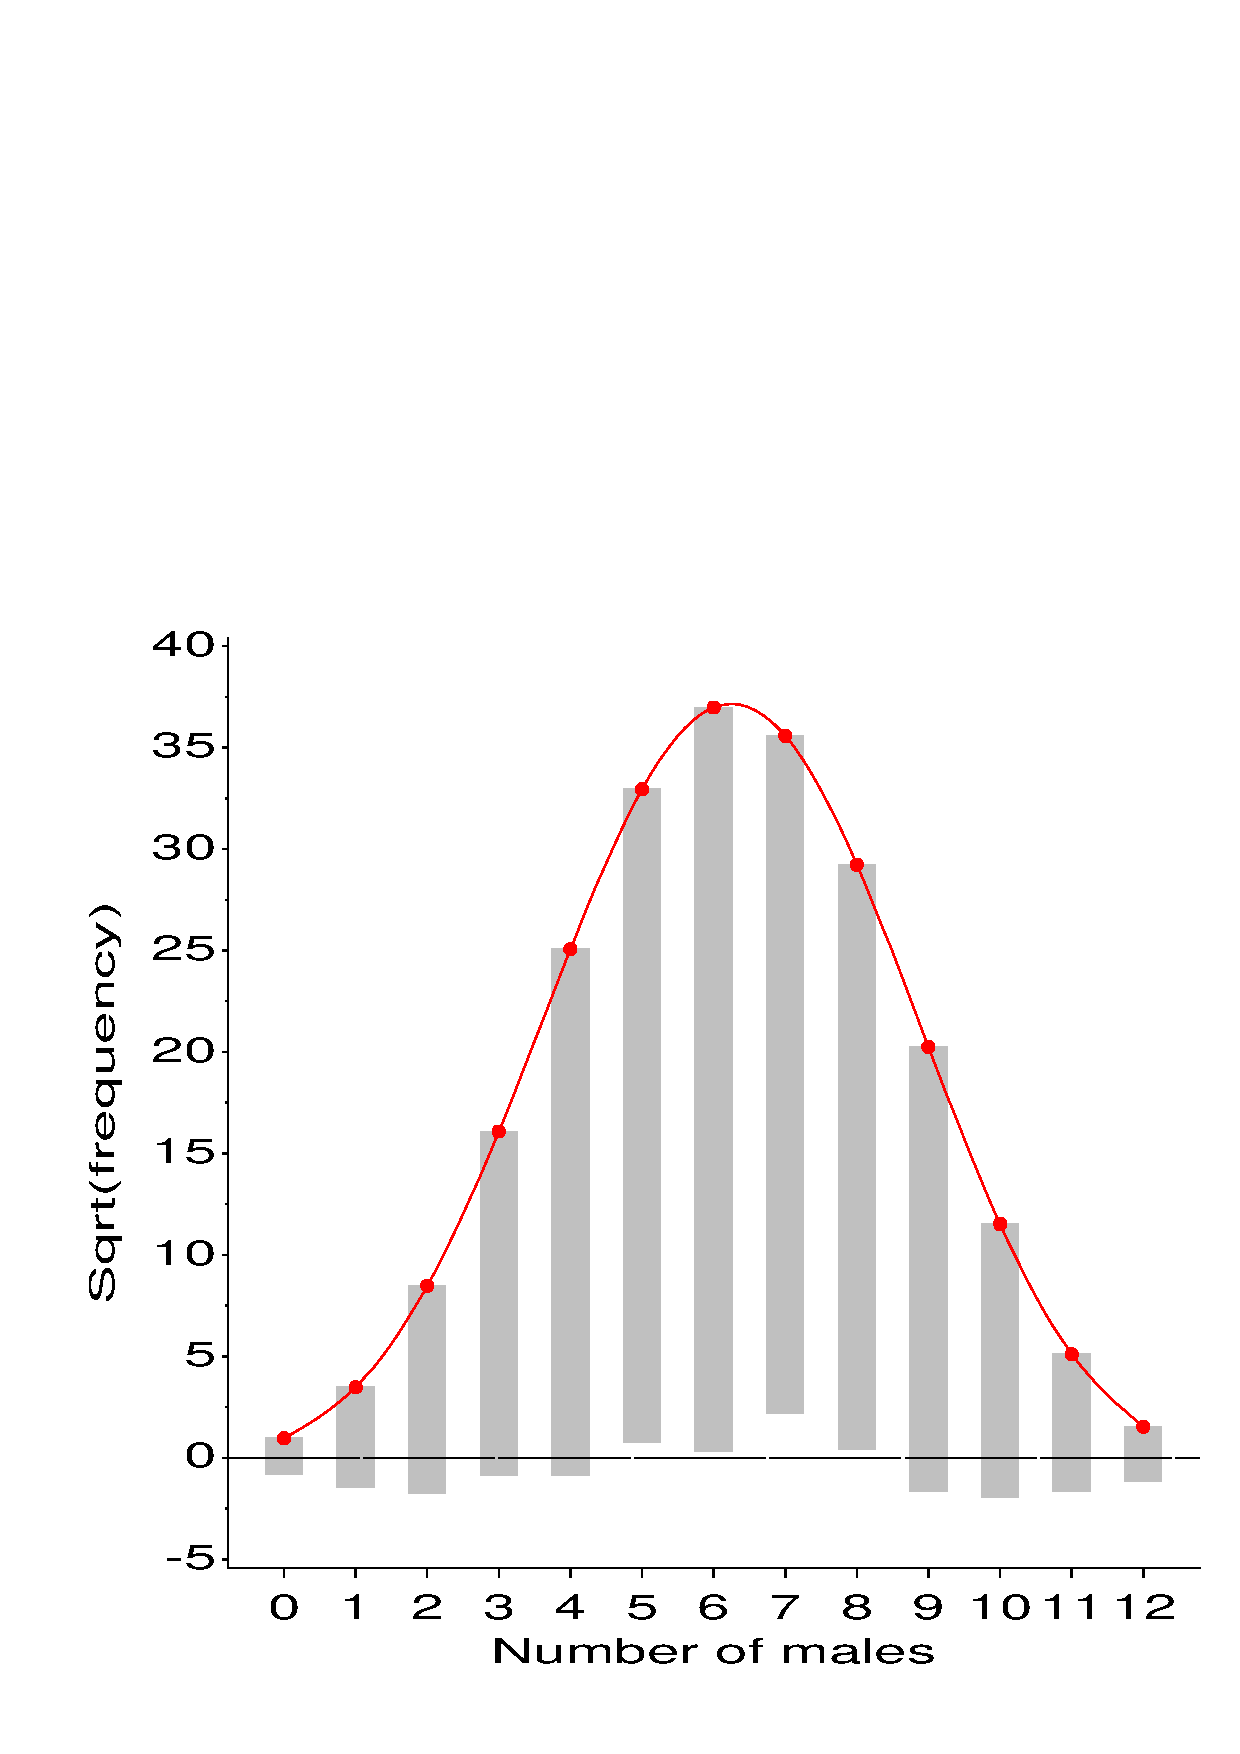
\includegraphics[width=1\linewidth]{saxony}\graphicsfile{ch2/fig/saxony.eps}{}
 \end{minipage}%
 \hfill
 \begin{minipage}[c]{.33\linewidth}
  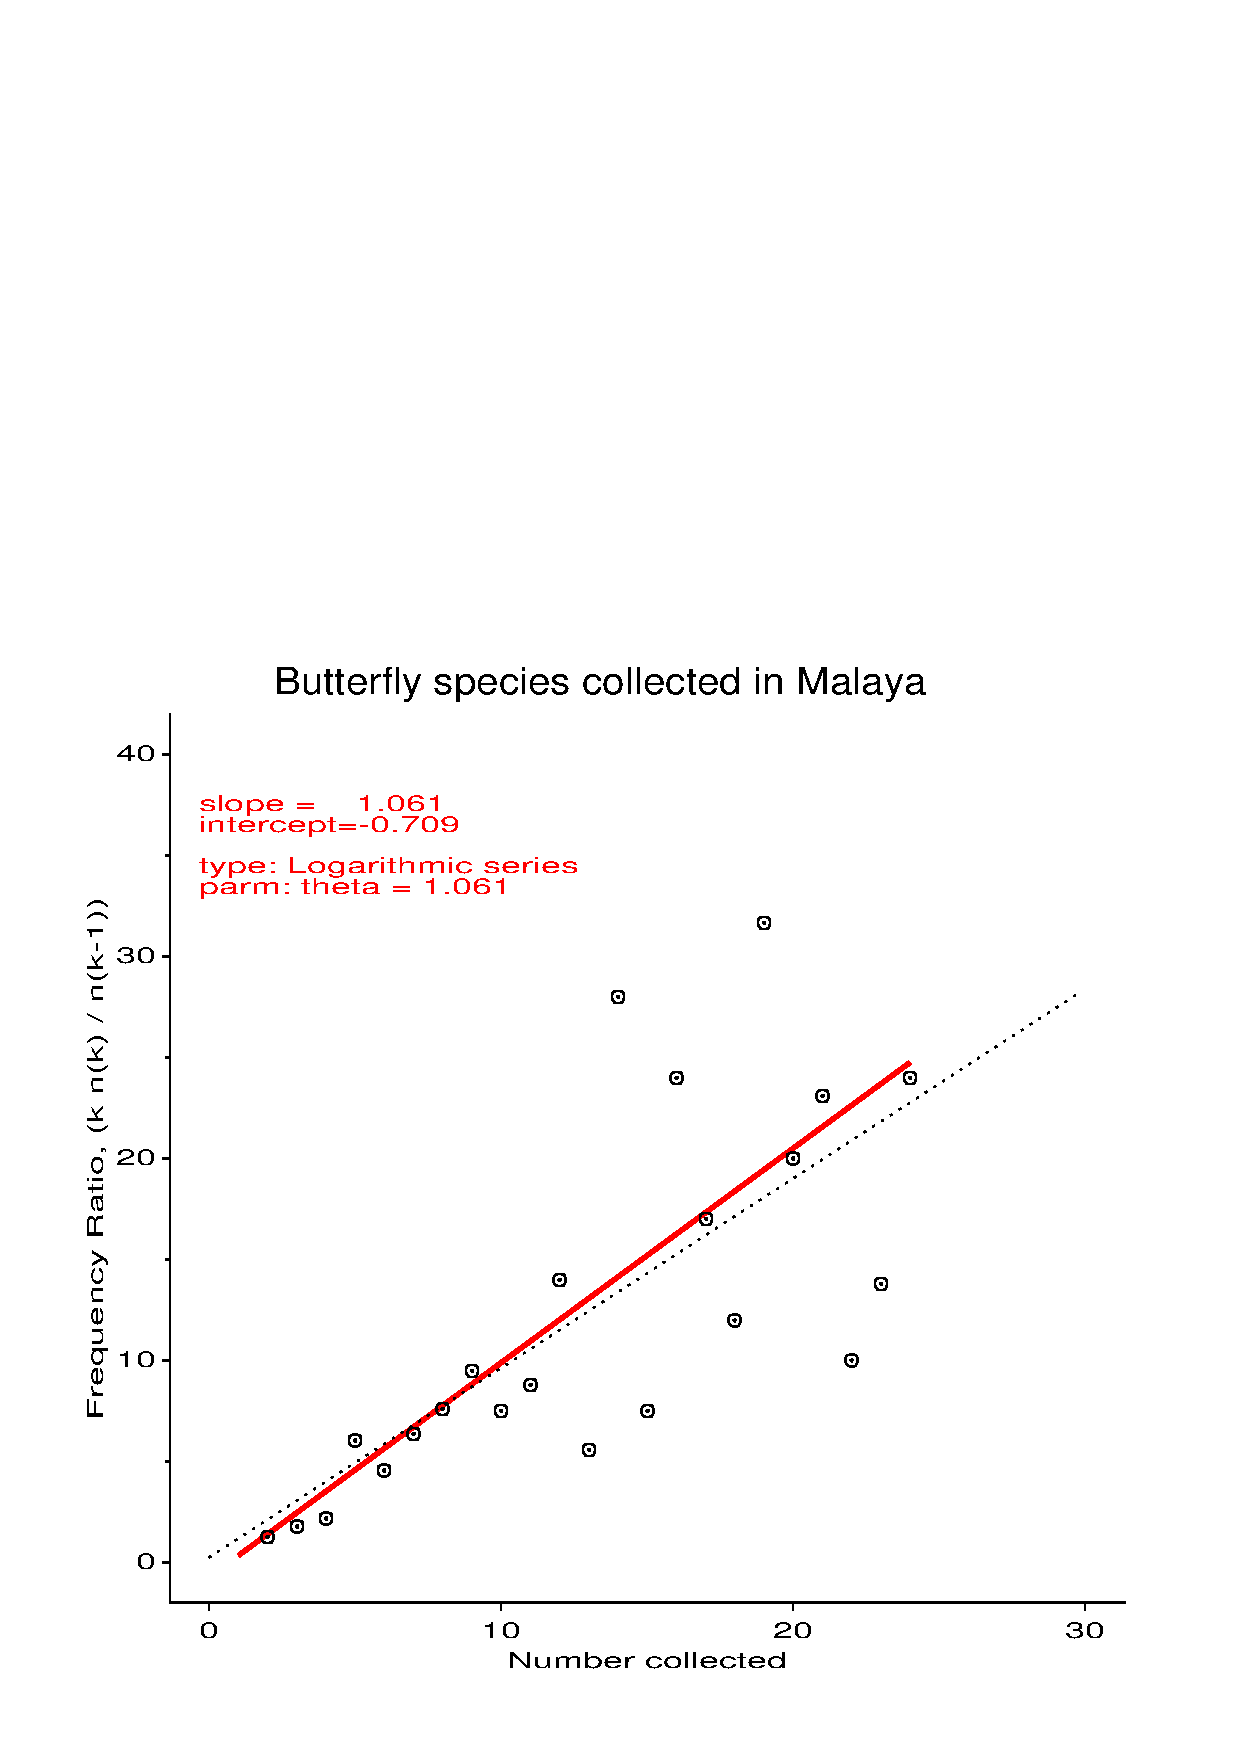
\includegraphics[width=1\linewidth]{orddemo3}\graphicsfile{ch2/fig/orddemo3.eps}{}
 \end{minipage}
 \hfill
 \begin{minipage}[c]{.33\linewidth}
  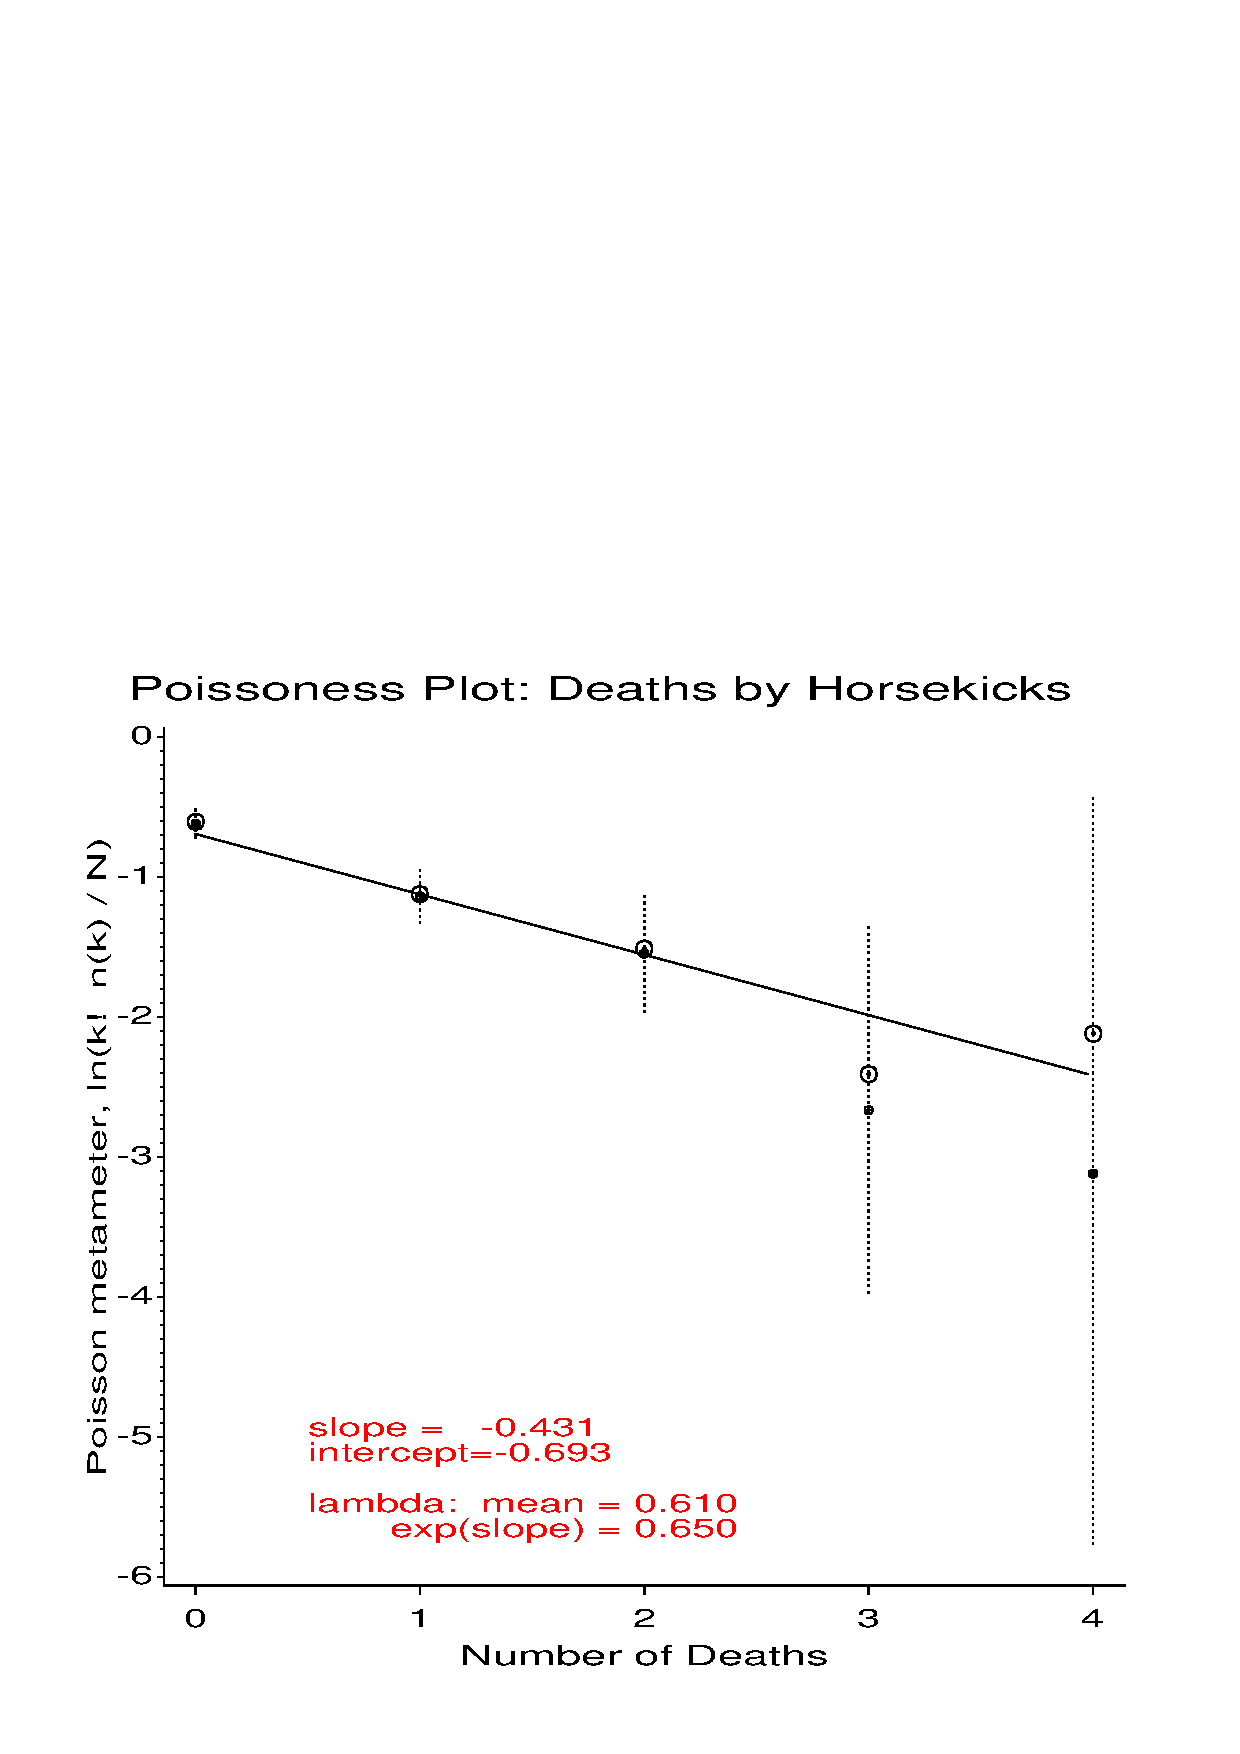
\includegraphics[width=1\linewidth]{poisdemo1}\graphicsfile{ch2/fig/poisdemo1.eps}{}
 \end{minipage}
\end{center}

   %% visual contents images

\chapterprelude{
Creating and manipulating categorical data sets requires
some skills and techniques in \R beyond those ordinarily used
for quantitative data. This chapter illustrates these for the
main formats for categorical data: case form, frequency form
and table form.
}

Categorical data can be represented as data sets
in various formats:
case form, frequency form, and table form.  This chapter
describes and illustrates the skills and techniques in \R
needed to input, create and manipulate \R data objects
to represent categorical data, and convert these from one
form to another for the purposes of statistical analysis
and visualization which are the subject of the remainder of the book.

As mentioned earlier, this book assumes that you have at least a
basic knowledge of the \R language and environment, including
interacting with the \R console (Rgui for Windows, R.app for Mac OS X)
or some other graphical user interface (e.g., RStudio),
loading and using \R functions in packages (e.g., \code{library(vcd)})
getting help for these from \R (e.g., \code{help(matrix)}), etc.
This chapter is therefore devoted
to covering those topics beyond such basic skills needed in the book.%
\footnote{
Some excellent introductory treatments of \R are:
\citet[\C 2]{FoxWeisberg:2011}, ...
Tom Short's \emph{R Reference Card}, \url{http://cran.us.r-project.org/doc/contrib/Short-refcard.pdf} is a handy 4-page summary of the main functions.
The web sites
Quick-R \url{http://www.statmethods.net/} and
Cookbook for R \url{http://www.cookbook-r.com/}
provide very helpful examples, organized by topics and tasks.
}


\section{Working with \R data: vectors, matrices, arrays and data frames}\label{sec:Rdata}

\R has a wide variety of data structures for storing, manipulating and
calculating with data.  Among these, vectors, matrices, arrays and
data frames are most important for the material in this book. 

In \R, a \term{vector} is a collection of values, like numbers, character strings, logicals (\code{TRUE, FALSE}) 
or dates, and often correspond to a variable in some analysis.
Matrices are rectangular arrays like a traditional table, composed of vectors in their columns
or rows.  
Arrays add additional dimensions, so that, for example, a 3-way table can be represented
as composed of rows, columns and layers.
An important consideration is that the values in vectors,
matrices and arrays must all be of the same \emph{mode}, e.g., numbers or character strings.
A \term{data frame} is a rectangular table, like a traditional data set in other
statistical environments, and composed of rows and columns like a matrix,
but allowing variables (columns) of different types. These data structures and the types of
data they can contain are illustrated in \figref{fig:datatypes}.

\begin{figure}
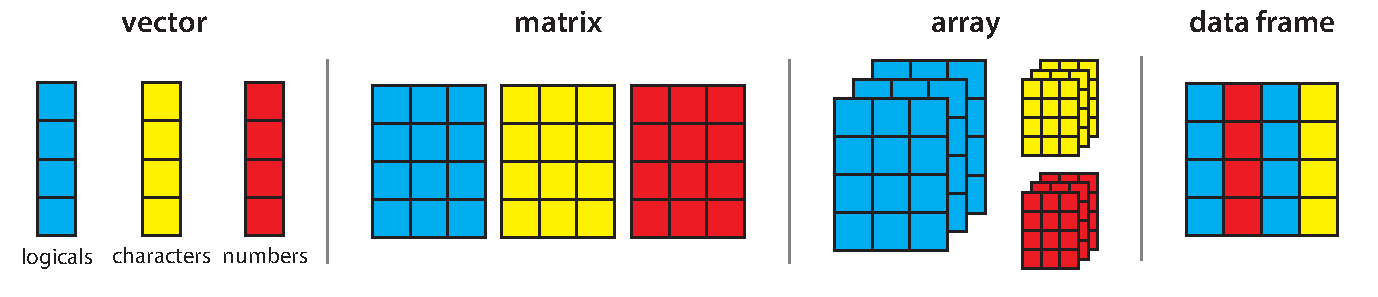
\includegraphics[width=\textwidth]{ch02/fig/datatypes2}
\caption[Principal data structures and data types in R]{Principal data structures and data types in \R.}
\label{fig:datatypes}
\end{figure}
\subsection{Vectors}
The simplest data structure in \R is a \term{vector}, a one-dimensional
collection of elements of the same type. An easy way to create a vector is with
the \func{c}, which combines its arguments.  The following examples create
and print vectors of length 4, containing numbers, character strings and
logical values respectively:

\begin{knitrout}
\definecolor{shadecolor}{rgb}{0.969, 0.969, 0.969}\color{fgcolor}\begin{kframe}
\begin{alltt}
\hlkwd{c}\hlstd{(}\hlnum{17}\hlstd{,} \hlnum{20}\hlstd{,} \hlnum{15}\hlstd{,} \hlnum{40}\hlstd{)}
\end{alltt}
\begin{verbatim}
## [1] 17 20 15 40
\end{verbatim}
\begin{alltt}
\hlkwd{c}\hlstd{(}\hlstr{"female"}\hlstd{,} \hlstr{"male"}\hlstd{,} \hlstr{"female"}\hlstd{,} \hlstr{"male"}\hlstd{)}
\end{alltt}
\begin{verbatim}
## [1] "female" "male"   "female" "male"
\end{verbatim}
\begin{alltt}
\hlkwd{c}\hlstd{(}\hlnum{TRUE}\hlstd{,} \hlnum{TRUE}\hlstd{,} \hlnum{FALSE}\hlstd{,} \hlnum{FALSE}\hlstd{)}
\end{alltt}
\begin{verbatim}
## [1]  TRUE  TRUE FALSE FALSE
\end{verbatim}
\end{kframe}
\end{knitrout}


To store these values in variables, \R uses the assignment operator (\code{<-})
or equals sign (\code{=}). This creates a variable named on the left-hand side.
An assignment doesn't print the result, but a bare expression does, so you can
assign and print by surrounding the assignment with \code{()}.

\begin{knitrout}
\definecolor{shadecolor}{rgb}{0.969, 0.969, 0.969}\color{fgcolor}\begin{kframe}
\begin{alltt}
\hlstd{count} \hlkwb{<-} \hlkwd{c}\hlstd{(}\hlnum{17}\hlstd{,} \hlnum{20}\hlstd{,} \hlnum{15}\hlstd{,} \hlnum{40}\hlstd{)}                       \hlcom{# assign}
\hlstd{count}                                            \hlcom{# print}
\end{alltt}
\begin{verbatim}
## [1] 17 20 15 40
\end{verbatim}
\begin{alltt}
\hlstd{(sex} \hlkwb{<-} \hlkwd{c}\hlstd{(}\hlstr{"female"}\hlstd{,} \hlstr{"male"}\hlstd{,} \hlstr{"female"}\hlstd{,} \hlstr{"male"}\hlstd{))}   \hlcom{# both}
\end{alltt}
\begin{verbatim}
## [1] "female" "male"   "female" "male"
\end{verbatim}
\begin{alltt}
\hlstd{(passed} \hlkwb{<-} \hlkwd{c}\hlstd{(}\hlnum{TRUE}\hlstd{,} \hlnum{TRUE}\hlstd{,} \hlnum{FALSE}\hlstd{,} \hlnum{FALSE}\hlstd{))}
\end{alltt}
\begin{verbatim}
## [1]  TRUE  TRUE FALSE FALSE
\end{verbatim}
\end{kframe}
\end{knitrout}


Other useful functions for creating vectors are:
\begin{itemize*}
  \item The \code{:} operator for generating consecutive integer sequences, e.g.,
  \code{1:10} gives the integers 1 to 10.  The \func{seq} function is more general, taking the forms
\code{seq(from, to)},
\code{seq(from, to, by= )}, and
\code{seq(from, to, length= )} where the optional argument \code{by} specifies the interval between adjacent values and \code{length} gives the desired length of the
result.

  \item The \func{rep} function generates repeated sequences, replicating
  its first argument (which may be a vector) a given number of \code{times},
  to a given \code{length} or \code{each} a given multiple.
\end{itemize*}

\begin{knitrout}
\definecolor{shadecolor}{rgb}{0.969, 0.969, 0.969}\color{fgcolor}\begin{kframe}
\begin{alltt}
\hlkwd{seq}\hlstd{(}\hlnum{10}\hlstd{,} \hlnum{100}\hlstd{,} \hlkwc{by}\hlstd{=}\hlnum{10}\hlstd{)}      \hlcom{# give interval}
\end{alltt}
\begin{verbatim}
##  [1]  10  20  30  40  50  60  70  80  90 100
\end{verbatim}
\begin{alltt}
\hlkwd{seq}\hlstd{(}\hlnum{0}\hlstd{,} \hlnum{1}\hlstd{,} \hlkwc{length}\hlstd{=}\hlnum{11}\hlstd{)}     \hlcom{# give length}
\end{alltt}
\begin{verbatim}
##  [1] 0.0 0.1 0.2 0.3 0.4 0.5 0.6 0.7 0.8 0.9 1.0
\end{verbatim}
\begin{alltt}
\hlstd{(sex} \hlkwb{<-} \hlkwd{rep}\hlstd{(}\hlkwd{c}\hlstd{(}\hlstr{"female"}\hlstd{,} \hlstr{"male"}\hlstd{),} \hlkwc{times}\hlstd{=}\hlnum{2}\hlstd{))}
\end{alltt}
\begin{verbatim}
## [1] "female" "male"   "female" "male"
\end{verbatim}
\begin{alltt}
\hlstd{(sex} \hlkwb{<-} \hlkwd{rep}\hlstd{(}\hlkwd{c}\hlstd{(}\hlstr{"female"}\hlstd{,} \hlstr{"male"}\hlstd{),} \hlkwc{length.out}\hlstd{=}\hlnum{4}\hlstd{))}  \hlcom{# same}
\end{alltt}
\begin{verbatim}
## [1] "female" "male"   "female" "male"
\end{verbatim}
\begin{alltt}
\hlstd{(passed} \hlkwb{<-} \hlkwd{rep}\hlstd{(}\hlkwd{c}\hlstd{(}\hlnum{TRUE}\hlstd{,} \hlnum{FALSE}\hlstd{),} \hlkwc{each}\hlstd{=}\hlnum{2}\hlstd{))}
\end{alltt}
\begin{verbatim}
## [1]  TRUE  TRUE FALSE FALSE
\end{verbatim}
\end{kframe}
\end{knitrout}


\subsection{Matrices}
A \term{matrix} is a two-dimensional array of elements of the same type composed
in a rectangular array of rows and columns. Matrices can be created by the function
\code{matrix(values, nrow, ncol)}, which takes the reshapes the elements in 
the first argument (\code{values}) to a matrix with \code{nrow} rows and
\code{ncol} columns. By default, the elements are filled in columnwise, unless
the optional argument \code{byrow=TRUE} is given.

\begin{knitrout}
\definecolor{shadecolor}{rgb}{0.969, 0.969, 0.969}\color{fgcolor}\begin{kframe}
\begin{alltt}
\hlstd{(matA} \hlkwb{<-} \hlkwd{matrix}\hlstd{(}\hlnum{1}\hlopt{:}\hlnum{8}\hlstd{,} \hlkwc{nrow}\hlstd{=}\hlnum{2}\hlstd{,} \hlkwc{ncol}\hlstd{=}\hlnum{4}\hlstd{))}
\end{alltt}
\begin{verbatim}
##      [,1] [,2] [,3] [,4]
## [1,]    1    3    5    7
## [2,]    2    4    6    8
\end{verbatim}
\begin{alltt}
\hlstd{(matB} \hlkwb{<-} \hlkwd{matrix}\hlstd{(}\hlnum{1}\hlopt{:}\hlnum{8}\hlstd{,} \hlkwc{nrow}\hlstd{=}\hlnum{2}\hlstd{,} \hlkwc{ncol}\hlstd{=}\hlnum{4}\hlstd{,} \hlkwc{byrow}\hlstd{=}\hlnum{TRUE}\hlstd{))}
\end{alltt}
\begin{verbatim}
##      [,1] [,2] [,3] [,4]
## [1,]    1    2    3    4
## [2,]    5    6    7    8
\end{verbatim}
\begin{alltt}
\hlstd{(matC} \hlkwb{<-} \hlkwd{matrix}\hlstd{(}\hlnum{1}\hlopt{:}\hlnum{4}\hlstd{,} \hlkwc{nrow}\hlstd{=}\hlnum{2}\hlstd{,} \hlkwc{ncol}\hlstd{=}\hlnum{4}\hlstd{))}
\end{alltt}
\begin{verbatim}
##      [,1] [,2] [,3] [,4]
## [1,]    1    3    1    3
## [2,]    2    4    2    4
\end{verbatim}
\end{kframe}
\end{knitrout}

\noindent The last example illustrates that the values in the first argument are recycled
as necessary to fill the given number of rows and columns.

All matrices have a dimensions attribute, a vector of length two giving the number
of rows and columns, retrieved with the function \func{dim}. Labels for the rows and
columns can be assigned using \func{dimnames},%
\footnote{
The \code{dimnames} can also be specified as an optional argument to \func{matrix}.
}
which takes a list of two vectors for the
row names and column names respectively. To see the structure of a matrix
(or any other \R object) and its attributes, I frequently use the \func{str} function,
as shown in the example below.

\begin{knitrout}
\definecolor{shadecolor}{rgb}{0.969, 0.969, 0.969}\color{fgcolor}\begin{kframe}
\begin{alltt}
\hlkwd{dim}\hlstd{(matA)}
\end{alltt}
\begin{verbatim}
## [1] 2 4
\end{verbatim}
\begin{alltt}
\hlkwd{str}\hlstd{(matA)}
\end{alltt}
\begin{verbatim}
##  int [1:2, 1:4] 1 2 3 4 5 6 7 8
\end{verbatim}
\begin{alltt}
\hlkwd{dimnames}\hlstd{(matA)} \hlkwb{<-} \hlkwd{list}\hlstd{(}\hlkwd{c}\hlstd{(}\hlstr{"M"}\hlstd{,}\hlstr{"F"}\hlstd{), LETTERS[}\hlnum{1}\hlopt{:}\hlnum{4}\hlstd{])}
\hlstd{matA}
\end{alltt}
\begin{verbatim}
##   A B C D
## M 1 3 5 7
## F 2 4 6 8
\end{verbatim}
\begin{alltt}
\hlkwd{str}\hlstd{(matA)}
\end{alltt}
\begin{verbatim}
##  int [1:2, 1:4] 1 2 3 4 5 6 7 8
##  - attr(*, "dimnames")=List of 2
##   ..$ : chr [1:2] "M" "F"
##   ..$ : chr [1:4] "A" "B" "C" "D"
\end{verbatim}
\end{kframe}
\end{knitrout}

Additionally, names for the row and column \emph{variables} themselves can also be assigned in the
\code{dimnames} call by giving each dimension vector a name.
\begin{knitrout}
\definecolor{shadecolor}{rgb}{0.969, 0.969, 0.969}\color{fgcolor}\begin{kframe}
\begin{alltt}
\hlkwd{dimnames}\hlstd{(matA)} \hlkwb{<-} \hlkwd{list}\hlstd{(}\hlkwc{sex}\hlstd{=}\hlkwd{c}\hlstd{(}\hlstr{"M"}\hlstd{,}\hlstr{"F"}\hlstd{),} \hlkwc{group}\hlstd{=LETTERS[}\hlnum{1}\hlopt{:}\hlnum{4}\hlstd{])}
\hlstd{matA}
\end{alltt}
\begin{verbatim}
##    group
## sex A B C D
##   M 1 3 5 7
##   F 2 4 6 8
\end{verbatim}
\begin{alltt}
\hlkwd{str}\hlstd{(matA)}
\end{alltt}
\begin{verbatim}
##  int [1:2, 1:4] 1 2 3 4 5 6 7 8
##  - attr(*, "dimnames")=List of 2
##   ..$ sex  : chr [1:2] "M" "F"
##   ..$ group: chr [1:4] "A" "B" "C" "D"
\end{verbatim}
\end{kframe}
\end{knitrout}


Matrices can also be created or enlarged by ``binding'' vectors or matrices together
by rows or columns:
\begin{itemize*}
  \item \code{rbind(a, b, c)} creates a matrix with the vectors \code{a}, \code{b} and \code{c} as its rows, recycling the elements as necessary to the length of the longest one.
  \item \code{cbind(a, b, c)} creates a matrix with the vectors \code{a}, \code{b} and \code{c} as its columns.
  \item \code{rbind(mat, a, b, ...)} and \code{cbind(mat, a, b, ...)} add additional
  rows (columns) to a matrix \code{mat}, recycling or subsetting the elements in the
  vectors to conform with the size of the matrix.
\end{itemize*}

\begin{knitrout}
\definecolor{shadecolor}{rgb}{0.969, 0.969, 0.969}\color{fgcolor}\begin{kframe}
\begin{alltt}
\hlkwd{rbind}\hlstd{(matA,} \hlkwd{c}\hlstd{(}\hlnum{10}\hlstd{,}\hlnum{20}\hlstd{))}
\end{alltt}
\begin{verbatim}
##    A  B  C  D
## M  1  3  5  7
## F  2  4  6  8
##   10 20 10 20
\end{verbatim}
\begin{alltt}
\hlkwd{cbind}\hlstd{(matA,} \hlkwd{c}\hlstd{(}\hlnum{10}\hlstd{,}\hlnum{20}\hlstd{))}
\end{alltt}
\begin{verbatim}
##   A B C D   
## M 1 3 5 7 10
## F 2 4 6 8 20
\end{verbatim}
\end{kframe}
\end{knitrout}


\subsection{Arrays}
Higher-dimensional arrays are less frequently encountered in traditional data analysis,
but they are of great use for categorical data, where frequency tables of three or more
variables can be naturally represented as arrays, with one dimension for each
table variable.

The function \code{array(values, dim)} takes the elements in \code{values} and
reshapes these into an array whose dimensions are given in the vector \code{dim}.
The number of dimensions is the length of \code{dim}.  As with matrices, the
elements are filled in with the first dimension (rows) varying most rapidly,
then by the second dimension (columns) and so on for all further dimensions,
which can be considered as layers.
A matrix is just the special case of an array with two dimensions.

\begin{knitrout}
\definecolor{shadecolor}{rgb}{0.969, 0.969, 0.969}\color{fgcolor}\begin{kframe}
\begin{alltt}
\hlstd{(arrayA} \hlkwb{<-} \hlkwd{array}\hlstd{(}\hlnum{1}\hlopt{:}\hlnum{16}\hlstd{,} \hlkwc{dim}\hlstd{=}\hlkwd{c}\hlstd{(}\hlnum{2}\hlstd{,} \hlnum{4}\hlstd{,} \hlnum{2}\hlstd{)))}     \hlcom{# 2 rows, 4 columns, 2 layers}
\end{alltt}
\begin{verbatim}
## , , 1
## 
##      [,1] [,2] [,3] [,4]
## [1,]    1    3    5    7
## [2,]    2    4    6    8
## 
## , , 2
## 
##      [,1] [,2] [,3] [,4]
## [1,]    9   11   13   15
## [2,]   10   12   14   16
\end{verbatim}
\begin{alltt}
\hlkwd{str}\hlstd{(arrayA)}
\end{alltt}
\begin{verbatim}
##  int [1:2, 1:4, 1:2] 1 2 3 4 5 6 7 8 9 10 ...
\end{verbatim}
\begin{alltt}
\hlstd{(arrayB} \hlkwb{<-} \hlkwd{array}\hlstd{(}\hlnum{1}\hlopt{:}\hlnum{16}\hlstd{,} \hlkwc{dim}\hlstd{=}\hlkwd{c}\hlstd{(}\hlnum{2}\hlstd{,} \hlnum{8}\hlstd{)))}        \hlcom{# 2 rows, 8 columns}
\end{alltt}
\begin{verbatim}
##      [,1] [,2] [,3] [,4] [,5] [,6] [,7] [,8]
## [1,]    1    3    5    7    9   11   13   15
## [2,]    2    4    6    8   10   12   14   16
\end{verbatim}
\begin{alltt}
\hlkwd{str}\hlstd{(arrayB)}
\end{alltt}
\begin{verbatim}
##  int [1:2, 1:8] 1 2 3 4 5 6 7 8 9 10 ...
\end{verbatim}
\end{kframe}
\end{knitrout}

In the same way that we can assign labels to the rows, columns and variables
in matrices, we can assign these attributes to \code{dimnames(arrayA)}, or
include this information in a \code{dimnames=} argument to \func{array}.

\begin{knitrout}
\definecolor{shadecolor}{rgb}{0.969, 0.969, 0.969}\color{fgcolor}\begin{kframe}
\begin{alltt}
\hlkwd{dimnames}\hlstd{(arrayA)} \hlkwb{<-} \hlkwd{list}\hlstd{(}\hlkwc{sex}\hlstd{=}\hlkwd{c}\hlstd{(}\hlstr{"M"}\hlstd{,} \hlstr{"F"}\hlstd{),}
                         \hlkwc{group}\hlstd{=letters[}\hlnum{1}\hlopt{:}\hlnum{4}\hlstd{],}
                         \hlkwc{time}\hlstd{=}\hlkwd{c}\hlstd{(}\hlstr{"Pre"}\hlstd{,} \hlstr{"Post"}\hlstd{))}
\hlstd{arrayA}
\end{alltt}
\begin{verbatim}
## , , time = Pre
## 
##    group
## sex a b c d
##   M 1 3 5 7
##   F 2 4 6 8
## 
## , , time = Post
## 
##    group
## sex  a  b  c  d
##   M  9 11 13 15
##   F 10 12 14 16
\end{verbatim}
\begin{alltt}
\hlkwd{str}\hlstd{(arrayA)}
\end{alltt}
\begin{verbatim}
##  int [1:2, 1:4, 1:2] 1 2 3 4 5 6 7 8 9 10 ...
##  - attr(*, "dimnames")=List of 3
##   ..$ sex  : chr [1:2] "M" "F"
##   ..$ group: chr [1:4] "a" "b" "c" "d"
##   ..$ time : chr [1:2] "Pre" "Post"
\end{verbatim}
\end{kframe}
\end{knitrout}

Arrays in \R can contain any single type of elements--- numbers,
character strings, logicals.  \R also has a variety of functions
(e.g., \func{table}, \func{xtabs})
for creating and manipulating \class{table} objects, which are 
specialized forms of matrices and arrays containing integer
frequencies in a contingency table. These are discussed in more
detail below (\secref{sec:table}).

\subsection{data frames}\label{sec:data-frames}
Data frames are the most commonly used form of data in \R and more
general than matrices in that they can contain columns of different types.
For statistical modeling, data frames play a special role, in that
many modeling functions are designed to take a data frame as a
\code{data=} argument, and then find the variables mentioned within
that data frame. Another distinguishing feature is that discrete variables
(columns) like character strings \code{("M", "F")} or integers \code{(1, 2, 3)}
in data frames can be represented as \term{factor}s, which simplifies
many statistical and graphical methods.

A data frame can be created using keyboard input 
with the \func{data.frame} function, applied to a list of objects,
\code{data.frame(a, b, c, ...)}, each of which can be a vector, matrix or another
data frame, but typically all containing the same number of rows.
This works roughly like \func{cbind}, collecting the arguments as columns
in the result.

The following example generates \code{n=100} random observations on 
three discrete factor variables, \code{A, B, sex}, and a numeric
variable, \code{age}.  As constructed, all of these are 
statistically independent, since none depends on any of the others.
The function \func{sample}
is used here to generate \code{n} random samples from the
first argument allowing replacement (\code{rep=TRUE}).
Finally, all four variables are combined into the data frame
\code{mydata}.


\begin{knitrout}
\definecolor{shadecolor}{rgb}{0.969, 0.969, 0.969}\color{fgcolor}\begin{kframe}
\begin{alltt}
\hlkwd{set.seed}\hlstd{(}\hlnum{12345}\hlstd{)}   \hlcom{# reproducibility}
\hlstd{n}\hlkwb{=}\hlnum{100}
\hlstd{A} \hlkwb{<-} \hlkwd{factor}\hlstd{(}\hlkwd{sample}\hlstd{(}\hlkwd{c}\hlstd{(}\hlstr{"a1"}\hlstd{,}\hlstr{"a2"}\hlstd{), n,} \hlkwc{rep}\hlstd{=}\hlnum{TRUE}\hlstd{))}
\hlstd{B} \hlkwb{<-} \hlkwd{factor}\hlstd{(}\hlkwd{sample}\hlstd{(}\hlkwd{c}\hlstd{(}\hlstr{"b1"}\hlstd{,}\hlstr{"b2"}\hlstd{), n,} \hlkwc{rep}\hlstd{=}\hlnum{TRUE}\hlstd{))}
\hlstd{sex} \hlkwb{<-} \hlkwd{factor}\hlstd{(}\hlkwd{sample}\hlstd{(}\hlkwd{c}\hlstd{(}\hlstr{"M"}\hlstd{,} \hlstr{"F"}\hlstd{), n,} \hlkwc{rep}\hlstd{=}\hlnum{TRUE}\hlstd{))}
\hlstd{age} \hlkwb{<-} \hlkwd{round}\hlstd{(}\hlkwd{rnorm}\hlstd{(n,} \hlkwc{mean}\hlstd{=}\hlnum{30}\hlstd{,} \hlkwc{sd}\hlstd{=}\hlnum{5}\hlstd{))}
\hlstd{mydata} \hlkwb{<-} \hlkwd{data.frame}\hlstd{(A, B, sex, age)}
\hlkwd{head}\hlstd{(mydata,}\hlnum{5}\hlstd{)}
\end{alltt}
\begin{verbatim}
##    A  B sex age
## 1 a2 b1   F  22
## 2 a2 b2   F  33
## 3 a2 b2   M  31
## 4 a2 b2   F  26
## 5 a1 b2   F  29
\end{verbatim}
\begin{alltt}
\hlkwd{str}\hlstd{(mydata)}
\end{alltt}
\begin{verbatim}
## 'data.frame':	100 obs. of  4 variables:
##  $ A  : Factor w/ 2 levels "a1","a2": 2 2 2 2 1 1 1 2 2 2 ...
##  $ B  : Factor w/ 2 levels "b1","b2": 1 2 2 2 2 2 2 2 1 1 ...
##  $ sex: Factor w/ 2 levels "F","M": 1 1 2 1 1 1 2 2 1 1 ...
##  $ age: num  22 33 31 26 29 29 38 28 30 27 ...
\end{verbatim}
\end{kframe}
\end{knitrout}


For real data sets, it is usually most convenient to read these into \R
from external files, and this is easiest using plain text (ASCII) files
with one line per observation and fields separated by commas (or tabs),
and with a first header line giving the variable names-- called
\emph{comma-separated} or CSV format.
If your data is in the form of Excel, SAS, SPSS or other file format,
you can almost always export that data to CSV format first.%
\footnote{
The \Rpackage{foreign} contains specialized functions to \emph{directly} read
data stored by Minitab, SAS, SPSS, Stata, Systat and other software.
There are also a number of packages for reading (and writing)
Excel spreadsheets directly (\pkg{gdata}, \pkg{XLConnect}, \pkg{xlsx}).
The \R manual, \emph{R Data Import/Export} covers many other variations,
including data in relational data bases.
}

The function \func{read.table} has many options to control the details
of how the data are read and converted to variables in the data frame.
Among these some important options are:
\begin{description*}
  \item [\code{header}] indicates whether the first line contains
variable names. The default is \code{FALSE} unless the first line contains one fewer field
than the number of columns;
  \item[\code{sep}] (default: \code{""} meaning white space, i.e., one or more spaces, tabs or newlines) specifies the separator character between fields;
  \item[\code{stringsAsFactors}] (default: \code{TRUE}) determines whether character string variables should be converted to factors;
  \item[\code{na.strings}] (default: \code{"NA"}) one or more strings which are interpreted
  as missing data values (\code{NA});
\end{description*}
For delimited files, \func{read.csv} and \func{read.delim} are convenient wrappers
to \func{read.table}, with default values \code{sep=","} and \code{sep="\t"}
respectively, and
\code{header=TRUE}. 

\begin{Example}[ch2-arth-csv]{Arthritis treatment}

The file \code{Arthritis.csv} contains data in CSV format
from \citet{KochEdwards:88}, representing
a double-blind clinical trial investigating a new treatment for rheumatoid arthritis with 84 patients. The first (``header'') line gives the variable names.  Some of the
lines in the file are shown below, with \code{...} representing omitted lines:
{\small
\renewcommand{\baselinestretch}{.85}
%<<arth-csv, eval=FALSE, results='asis'>>=
\begin{verbatim}
ID,Treatment,Sex,Age,Improved
57,Treated,Male,27,Some
46,Treated,Male,29,None
77,Treated,Male,30,None
17,Treated,Male,32,Marked
 ...
42,Placebo,Female,66,None
15,Placebo,Female,66,Some
71,Placebo,Female,68,Some
1,Placebo,Female,74,Marked
\end{verbatim}
%@
}
We read this into \R using \func{read.csv} as shown below, using all the
default options:
\begin{knitrout}\footnotesize
\definecolor{shadecolor}{rgb}{0.969, 0.969, 0.969}\color{fgcolor}\begin{kframe}
\begin{alltt}
\hlstd{Arthritis} \hlkwb{<-} \hlkwd{read.csv}\hlstd{(}\hlstr{"ch02/Arthritis.csv"}\hlstd{)}
\hlkwd{str}\hlstd{(Arthritis)}
\end{alltt}
\begin{verbatim}
## 'data.frame':	84 obs. of  5 variables:
##  $ ID       : int  57 46 77 17 36 23 75 39 33 55 ...
##  $ Treatment: Factor w/ 2 levels "Placebo","Treated": 2 2 2 2 2 2 2 2 2 2 ...
##  $ Sex      : Factor w/ 2 levels "Female","Male": 2 2 2 2 2 2 2 2 2 2 ...
##  $ Age      : int  27 29 30 32 46 58 59 59 63 63 ...
##  $ Improved : Factor w/ 3 levels "Marked","None",..: 3 2 2 1 1 1 2 1 2 2 ...
\end{verbatim}
\end{kframe}
\end{knitrout}

Note that the character variables \var{Treatment}, \var{Sex} and \var{Improved}
were converted to factors, and the levels of those variables were
ordered \emph{alphabetically}.  This often doesn't matter much for binary variables,
but here, the response variable, \var{Improved} has levels
that should be considered \emph{ordered}, 
as \code{"None", "Some", "Marked"}.  We can correct this here by
re-assigning \code{Arthritis$Improved} using \func{ordered}.
The topic of re-ordering variables and levels in categorical data is
considered in more detail in \secref{sec:ordered}.

\begin{knitrout}
\definecolor{shadecolor}{rgb}{0.969, 0.969, 0.969}\color{fgcolor}\begin{kframe}
\begin{alltt}
\hlkwd{levels}\hlstd{(Arthritis}\hlopt{$}\hlstd{Improved)}
\end{alltt}
\begin{verbatim}
## [1] "Marked" "None"   "Some"
\end{verbatim}
\begin{alltt}
\hlstd{Arthritis}\hlopt{$}\hlstd{Improved} \hlkwb{<-} \hlkwd{ordered}\hlstd{(Arthritis}\hlopt{$}\hlstd{Improved,}
                              \hlkwc{levels}\hlstd{=}\hlkwd{c}\hlstd{(}\hlstr{"None"}\hlstd{,} \hlstr{"Some"}\hlstd{,} \hlstr{"Marked"}\hlstd{))}
\end{alltt}
\end{kframe}
\end{knitrout}


\end{Example}

\section{Forms of categorical data: case form, frequency form and table form}\label{sec:forms}
As we saw in \chref{ch:intro}, categorical data can be represented as ordinary data sets
in case form, but the discrete nature of factors or stratifying variables allows the same
information to be represented more compactly in summarized form with a frequency
variable for each cell of factor combinations, or in tables.  
Consequently, we sometimes 
find data created or presented in one form (e.g., a spreadsheet data set, a two-way
table of frequencies) and want to input that into \R.  Once we have the data in \R,
it is often necessary to manipulate the data into some other form for the purposes
of statistical analysis, visualizing results and our own presentation.
It is useful to understand the three main forms of categorical data in \R and how
to work with them for our purposes.

\subsection{Case form}
Categorical data in case form are simply data frames, with one or more discrete
classifying variables or response variables, most conveniently represented as factors or ordered factors.  In case form, the data set can also contain numeric variables
(covariates or other response variables), that cannot be accommodated in other
forms.

As with any data frame, \code{X}, you can access or compute with its attributes using \code{nrow(X)} for the number of observations,
\code{ncol(X)} for the number of variables, 
\code{names(X)} or \code{colnames(X)} for the variable names and
so forth.

\begin{Example}[ch2-arth]{Arthritis treatment}


The \data{Arthritis} data is available in case form in the \pkg{vcd} package. 
There are two explanatory factors: \code{Treatment} and \code{Sex}. \code{Age}
is a numeric covariate, and \code{Improved} is the response--- an ordered factor,
with levels 
%\code{paste(levels(Arthritis$Improved),collapse=' < ')}.  
\code{"None" < "Some" < "Marked"}.
Excluding \code{Age}, we would have
a $2 \times 2 \times 3$ contingency table for \code{Treatment}, \code{Sex} and \code{Improved}.
\begin{knitrout}\footnotesize
\definecolor{shadecolor}{rgb}{0.969, 0.969, 0.969}\color{fgcolor}\begin{kframe}
\begin{alltt}
\hlkwd{data}\hlstd{(Arthritis,} \hlkwc{package}\hlstd{=}\hlstr{"vcd"}\hlstd{)}  \hlcom{# load the data}
\hlkwd{names}\hlstd{(Arthritis)}      \hlcom{# show the variables}
\end{alltt}
\begin{verbatim}
## [1] "ID"        "Treatment" "Sex"       "Age"      
## [5] "Improved"
\end{verbatim}
\begin{alltt}
\hlkwd{str}\hlstd{(Arthritis)}        \hlcom{# show the structure}
\end{alltt}
\begin{verbatim}
## 'data.frame':	84 obs. of  5 variables:
##  $ ID       : int  57 46 77 17 36 23 75 39 33 55 ...
##  $ Treatment: Factor w/ 2 levels "Placebo","Treated": 2 2 2 2 2 2 2 2 2 2 ...
##  $ Sex      : Factor w/ 2 levels "Female","Male": 2 2 2 2 2 2 2 2 2 2 ...
##  $ Age      : int  27 29 30 32 46 58 59 59 63 63 ...
##  $ Improved : Ord.factor w/ 3 levels "None"<"Some"<..: 2 1 1 3 3 3 1 3 1 1 ...
\end{verbatim}
\begin{alltt}
\hlkwd{head}\hlstd{(Arthritis,}\hlnum{5}\hlstd{)}     \hlcom{# first 5 observations, same as Arthritis[1:5,] }
\end{alltt}
\begin{verbatim}
##   ID Treatment  Sex Age Improved
## 1 57   Treated Male  27     Some
## 2 46   Treated Male  29     None
## 3 77   Treated Male  30     None
## 4 17   Treated Male  32   Marked
## 5 36   Treated Male  46   Marked
\end{verbatim}
\end{kframe}
\end{knitrout}

\end{Example}

\subsection{Frequency form}
Data in frequency form is also a data frame, containing
one or more discrete factor variables and a frequency variable
(often called \code{Freq} or \code{count})
representing the number of basic observations in that cell.

This is an alternative representation of a table form data set considered
below.
In frequency form, the number of cells in the equivalent table
is \code{nrow{X}}, and the total number of observations
is the sum of the frequency variable, \code{sum(X$Freq)},
 \code{sum(X[,"Freq"])} or similar expression.

\begin{Example}[ch2-GSS]{General social survey} 
For small frequency tables, it is often convenient to enter them in frequency form
using \func{expand.grid} for the factors and \func{c} to list the counts in a vector.
The example below, from \cite{Agresti:2002} gives results for the 1991 General Social Survey,
with respondents classified by sex and party identification.
As a table, the data look like this:
\begin{center}
\begin{tabular}{rrrr}
  \hline
    &     & party & \\
  \hline
sex & dem & indep & rep \\ 
  \hline
female & 279 & 73 & 225 \\ 
  male & 165 & 47 & 191 \\ 
   \hline
\end{tabular}
\end{center}



We use \func{expand.grid} to create a $6 \times 2$ matrix
containing the combinations of \code{sex} and \code{party} 
with the levels for \code{sex} given first, so that this varies
most rapidly. Then,
input the frequencies in the table by columns from
left to right, and combine these two results with
\func{data.frame}.
\begin{knitrout}
\definecolor{shadecolor}{rgb}{0.969, 0.969, 0.969}\color{fgcolor}\begin{kframe}
\begin{alltt}
\hlcom{# Agresti (2002), table 3.11, p. 106}
\hlstd{GSS} \hlkwb{<-} \hlkwd{data.frame}\hlstd{(}
  \hlkwd{expand.grid}\hlstd{(}\hlkwc{sex}\hlstd{=}\hlkwd{c}\hlstd{(}\hlstr{"female"}\hlstd{,} \hlstr{"male"}\hlstd{),}
              \hlkwc{party}\hlstd{=}\hlkwd{c}\hlstd{(}\hlstr{"dem"}\hlstd{,} \hlstr{"indep"}\hlstd{,} \hlstr{"rep"}\hlstd{)),}
  \hlkwc{count}\hlstd{=}\hlkwd{c}\hlstd{(}\hlnum{279}\hlstd{,}\hlnum{165}\hlstd{,}\hlnum{73}\hlstd{,}\hlnum{47}\hlstd{,}\hlnum{225}\hlstd{,}\hlnum{191}\hlstd{))}
\hlstd{GSS}
\end{alltt}
\begin{verbatim}
##      sex party count
## 1 female   dem   279
## 2   male   dem   165
## 3 female indep    73
## 4   male indep    47
## 5 female   rep   225
## 6   male   rep   191
\end{verbatim}
\begin{alltt}
\hlkwd{names}\hlstd{(GSS)}
\end{alltt}
\begin{verbatim}
## [1] "sex"   "party" "count"
\end{verbatim}
\begin{alltt}
\hlkwd{str}\hlstd{(GSS)}
\end{alltt}
\begin{verbatim}
## 'data.frame':	6 obs. of  3 variables:
##  $ sex  : Factor w/ 2 levels "female","male": 1 2 1 2 1 2
##  $ party: Factor w/ 3 levels "dem","indep",..: 1 1 2 2 3 3
##  $ count: num  279 165 73 47 225 191
\end{verbatim}
\begin{alltt}
\hlkwd{sum}\hlstd{(GSS}\hlopt{$}\hlstd{count)}
\end{alltt}
\begin{verbatim}
## [1] 980
\end{verbatim}
\end{kframe}
\end{knitrout}

The last line above shows that there are 980
cases represented in the frequency table.
\end{Example}

\subsection{Table form}
Table form data is represented as a matrix, array or table object
whose elements are the frequencies in an $n$-way table.
The number of dimensions of the table is the length, 
\code{length(dim(X))}, of its
\code{dim} (or \code{dimnames}) attribute, and the sizes of the
dimensions in the table are the elements of \code{dim(X)}.
The total number of observations represented is the sum of
all the frequencies, \code{sum(X)}.

\begin{Example}[ch2-hec]{Hair-eye color data}
A classic data set on frequencies of hair color, eye color and
sex is given in table form in \code{HairEyeColor} in the 
\Rpackage{vcd}, reporting the frequencies of these
categories for \code{592} students in
a statistics course.
\begin{knitrout}
\definecolor{shadecolor}{rgb}{0.969, 0.969, 0.969}\color{fgcolor}\begin{kframe}
\begin{alltt}
\hlkwd{data}\hlstd{(HairEyeColor,} \hlkwc{package}\hlstd{=}\hlstr{"datasets"}\hlstd{)}    \hlcom{# load the data}
\hlkwd{str}\hlstd{(HairEyeColor)}                \hlcom{# show the structure}
\end{alltt}
\begin{verbatim}
##  table [1:4, 1:4, 1:2] 32 53 10 3 11 50 10 30 10 25 ...
##  - attr(*, "dimnames")=List of 3
##   ..$ Hair: chr [1:4] "Black" "Brown" "Red" "Blond"
##   ..$ Eye : chr [1:4] "Brown" "Blue" "Hazel" "Green"
##   ..$ Sex : chr [1:2] "Male" "Female"
\end{verbatim}
\begin{alltt}
\hlkwd{dim}\hlstd{(HairEyeColor)}                \hlcom{# table dimension sizes}
\end{alltt}
\begin{verbatim}
## [1] 4 4 2
\end{verbatim}
\begin{alltt}
\hlkwd{dimnames}\hlstd{(HairEyeColor)}           \hlcom{# variable and level names}
\end{alltt}
\begin{verbatim}
## $Hair
## [1] "Black" "Brown" "Red"   "Blond"
## 
## $Eye
## [1] "Brown" "Blue"  "Hazel" "Green"
## 
## $Sex
## [1] "Male"   "Female"
\end{verbatim}
\begin{alltt}
\hlkwd{sum}\hlstd{(HairEyeColor)}                \hlcom{# number of cases}
\end{alltt}
\begin{verbatim}
## [1] 592
\end{verbatim}
\end{kframe}
\end{knitrout}

Three-way (and higher-way) tables can be printed in a more convenient
form using \func{structable} and \func{ftable} as described below
in \secref{sec:structable}.
\end{Example}

Tables are often created from raw data in case form or frequency form using the
functions \func{table} and \func{xtabs} described in \secref{sec:table}.
For smallish frequency tables that are already in tabular form, you can enter
the frequencies in a matrix, and then assign \code{dimnames} and other attributes.

To illustrate, we create the GSS data as a table below, entering the
values in the table by rows (\code{byrow=TRUE}), as they appear in
printed form.

\begin{knitrout}
\definecolor{shadecolor}{rgb}{0.969, 0.969, 0.969}\color{fgcolor}\begin{kframe}
\begin{alltt}
\hlstd{GSS.tab} \hlkwb{<-} \hlkwd{matrix}\hlstd{(}\hlkwd{c}\hlstd{(}\hlnum{279}\hlstd{,} \hlnum{73}\hlstd{,} \hlnum{225}\hlstd{,}
                    \hlnum{165}\hlstd{,} \hlnum{47}\hlstd{,} \hlnum{191}\hlstd{),} \hlkwc{nrow}\hlstd{=}\hlnum{2}\hlstd{,} \hlkwc{ncol}\hlstd{=}\hlnum{3}\hlstd{,} \hlkwc{byrow}\hlstd{=}\hlnum{TRUE}\hlstd{)}
\hlkwd{dimnames}\hlstd{(GSS.tab)} \hlkwb{<-} \hlkwd{list}\hlstd{(}\hlkwc{sex}\hlstd{=}\hlkwd{c}\hlstd{(}\hlstr{"female"}\hlstd{,} \hlstr{"male"}\hlstd{),}
                          \hlkwc{party}\hlstd{=}\hlkwd{c}\hlstd{(}\hlstr{"dem"}\hlstd{,} \hlstr{"indep"}\hlstd{,} \hlstr{"rep"}\hlstd{))}
\hlstd{GSS.tab}
\end{alltt}
\begin{verbatim}
##         party
## sex      dem indep rep
##   female 279    73 225
##   male   165    47 191
\end{verbatim}
\end{kframe}
\end{knitrout}

\code{GSS.tab} is a matrix, not an object of \code{class("table")}, and some functions
are happier with tables than matrices.%
\footnote{
There are quite a few functions in \R with specialized methods for
\class{table} objects. For example, \code{plot(GSS.tab)} gives a mosaic
plot and \code{barchart(GSS.tab)} gives a divided bar chart.
}
You can coerce it to a table with \func{as.table},
\begin{knitrout}
\definecolor{shadecolor}{rgb}{0.969, 0.969, 0.969}\color{fgcolor}\begin{kframe}
\begin{alltt}
\hlstd{GSS.tab} \hlkwb{<-} \hlkwd{as.table}\hlstd{(GSS.tab)}
\hlkwd{str}\hlstd{(GSS.tab)}
\end{alltt}
\begin{verbatim}
##  table [1:2, 1:3] 279 165 73 47 225 191
##  - attr(*, "dimnames")=List of 2
##   ..$ sex  : chr [1:2] "female" "male"
##   ..$ party: chr [1:3] "dem" "indep" "rep"
\end{verbatim}
\end{kframe}
\end{knitrout}


Here is another similar example, entering data on job satisfactory
classified by \code{income} and level of \code{satisfaction}
from a $4 \times 4$ table given by \citet[Table 2.8, p. 57]{Agresti:2002}.
\begin{knitrout}
\definecolor{shadecolor}{rgb}{0.969, 0.969, 0.969}\color{fgcolor}\begin{kframe}
\begin{alltt}
\hlcom{## A 4 x 4 table  Agresti (2002, Table 2.8, p. 57) Job Satisfaction}
\hlstd{JobSat} \hlkwb{<-} \hlkwd{matrix}\hlstd{(}\hlkwd{c}\hlstd{(}\hlnum{1}\hlstd{,}\hlnum{2}\hlstd{,}\hlnum{1}\hlstd{,}\hlnum{0}\hlstd{,} \hlnum{3}\hlstd{,}\hlnum{3}\hlstd{,}\hlnum{6}\hlstd{,}\hlnum{1}\hlstd{,} \hlnum{10}\hlstd{,}\hlnum{10}\hlstd{,}\hlnum{14}\hlstd{,}\hlnum{9}\hlstd{,} \hlnum{6}\hlstd{,}\hlnum{7}\hlstd{,}\hlnum{12}\hlstd{,}\hlnum{11}\hlstd{),} \hlnum{4}\hlstd{,} \hlnum{4}\hlstd{)}
\hlkwd{dimnames}\hlstd{(JobSat)} \hlkwb{=} \hlkwd{list}\hlstd{(}\hlkwc{income}\hlstd{=}\hlkwd{c}\hlstd{(}\hlstr{"< 15k"}\hlstd{,} \hlstr{"15-25k"}\hlstd{,} \hlstr{"25-40k"}\hlstd{,} \hlstr{"> 40k"}\hlstd{),}
                \hlkwc{satisfaction}\hlstd{=}\hlkwd{c}\hlstd{(}\hlstr{"VeryD"}\hlstd{,} \hlstr{"LittleD"}\hlstd{,} \hlstr{"ModerateS"}\hlstd{,} \hlstr{"VeryS"}\hlstd{))}
\hlstd{JobSat} \hlkwb{<-} \hlkwd{as.table}\hlstd{(JobSat)}
\hlstd{JobSat}
\end{alltt}
\begin{verbatim}
##         satisfaction
## income   VeryD LittleD ModerateS VeryS
##   < 15k      1       3        10     6
##   15-25k     2       3        10     7
##   25-40k     1       6        14    12
##   > 40k      0       1         9    11
\end{verbatim}
\end{kframe}
\end{knitrout}



\section{Ordered factors and reordered tables}\label{sec:ordered}
As we saw above (\exref{ex:ch2-arth-csv}), factor variables in 
data frames (case form or frequency form)
can be re-ordered and declared as ordered factors using \func{ordered}.
As well, the order of the factors themselves can be rearranged by
sorting the data frame using \func{sort}.

However, in table form, the values of the table factors are ordered by their position in the table.
Thus in the \data{JobSat} data, both \code{income} and \code{satisfaction} represent ordered
factors, and the \emph{positions} of the values in the rows and columns reflects their
ordered nature, but only implicitly.

Yet, for analysis or graphing, there are occasions when you need \emph{numeric} values for the levels
of ordered factors in a table, e.g., to treat a factor as a quantitative variable.
In such cases, you can simply re-assign the \code{dimnames} attribute of the table
variables.  For example, here, we assign numeric values to \code{income} as the middle of their
ranges, and treat \code{satisfaction} as equally spaced with integer scores.

\begin{knitrout}
\definecolor{shadecolor}{rgb}{0.969, 0.969, 0.969}\color{fgcolor}\begin{kframe}
\begin{alltt}
\hlkwd{dimnames}\hlstd{(JobSat)}\hlopt{$}\hlstd{income} \hlkwb{<-} \hlkwd{c}\hlstd{(}\hlnum{7.5}\hlstd{,}\hlnum{20}\hlstd{,}\hlnum{32.5}\hlstd{,}\hlnum{60}\hlstd{)}
\hlkwd{dimnames}\hlstd{(JobSat)}\hlopt{$}\hlstd{satisfaction} \hlkwb{<-} \hlnum{1}\hlopt{:}\hlnum{4}
\end{alltt}
\end{kframe}
\end{knitrout}


A related case is when you want to preserve the character labels of table dimensions,
but also allow them to be sorted in some particular order. A simple way to do this
is to prefix each label with an integer index using \func{paste}.

\begin{knitrout}
\definecolor{shadecolor}{rgb}{0.969, 0.969, 0.969}\color{fgcolor}\begin{kframe}
\begin{alltt}
\hlkwd{dimnames}\hlstd{(JobSat)}\hlopt{$}\hlstd{income} \hlkwb{<-} \hlkwd{paste}\hlstd{(}\hlnum{1}\hlopt{:}\hlnum{4}\hlstd{,} \hlkwd{dimnames}\hlstd{(JobSat)}\hlopt{$}\hlstd{income,} \hlkwc{sep}\hlstd{=}\hlstr{":"}\hlstd{)}
\hlkwd{dimnames}\hlstd{(JobSat)}\hlopt{$}\hlstd{satisfaction} \hlkwb{<-}
                           \hlkwd{paste}\hlstd{(}\hlnum{1}\hlopt{:}\hlnum{4}\hlstd{,} \hlkwd{dimnames}\hlstd{(JobSat)}\hlopt{$}\hlstd{satisfaction,} \hlkwc{sep}\hlstd{=}\hlstr{":"}\hlstd{)}
\end{alltt}
\end{kframe}
\end{knitrout}


A different situation arises with tables where you want to \emph{permute} the levels
of one or more variables to arrange them in a more convenient order without changing
their labels. For example, in the \data{HairEyeColor} table, hair color and eye color are ordered arbitrarily.
For visualizing the data using mosaic plots and other methods described later, it 
turns out to be more useful to assure that both hair color and eye color are
ordered from dark to light.
Hair colors are actually ordered this way already:
\code{"Black", "Brown", "Red", "Blond"}.
But eye colors are ordered as \code{"Brown", "Blue", "Hazel", "Green"}.
It is easiest to re-order the
eye colors by indexing the columns (dimension 2) in this array to a new order,
\code{"Brown", "Hazel", "Green", "Blue"}, giving the
indices of the old levels in the new order (here: 1,3,4,2).
Again \func{str} is your friend, showing the structure of the result
to check that the result is what you want.

\begin{knitrout}
\definecolor{shadecolor}{rgb}{0.969, 0.969, 0.969}\color{fgcolor}\begin{kframe}
\begin{alltt}
\hlkwd{data}\hlstd{(HairEyeColor,} \hlkwc{package}\hlstd{=}\hlstr{"datasets"}\hlstd{)}
\hlstd{HEC} \hlkwb{<-} \hlstd{HairEyeColor[,} \hlkwd{c}\hlstd{(}\hlnum{1}\hlstd{,}\hlnum{3}\hlstd{,}\hlnum{4}\hlstd{,}\hlnum{2}\hlstd{), ]}
\hlkwd{str}\hlstd{(HEC)}
\end{alltt}
\begin{verbatim}
##  num [1:4, 1:4, 1:2] 32 53 10 3 10 25 7 5 3 15 ...
##  - attr(*, "dimnames")=List of 3
##   ..$ Hair: chr [1:4] "Black" "Brown" "Red" "Blond"
##   ..$ Eye : chr [1:4] "Brown" "Hazel" "Green" "Blue"
##   ..$ Sex : chr [1:2] "Male" "Female"
\end{verbatim}
\end{kframe}
\end{knitrout}

%This is also the order for both hair color and eye color shown in 
%the result of a correspondence analysis (\figref{fig:ca-haireye}) below.

Finally, there are situations where, particularly for display purposes, you
want to re-order the \emph{dimensions} of an $n$-way table, and/or change the
labels for the variables or levels.
This is easy when the data are in table form: \func{aperm} permutes
the dimensions, and assigning to \code{names} and \code{dimnames}
changes variable names and level labels respectively.

\begin{knitrout}
\definecolor{shadecolor}{rgb}{0.969, 0.969, 0.969}\color{fgcolor}\begin{kframe}
\begin{alltt}
\hlkwd{str}\hlstd{(UCBAdmissions)}
\end{alltt}
\begin{verbatim}
##  table [1:2, 1:2, 1:6] 512 313 89 19 353 207 17 8 120 205 ...
##  - attr(*, "dimnames")=List of 3
##   ..$ Admit : chr [1:2] "Admitted" "Rejected"
##   ..$ Gender: chr [1:2] "Male" "Female"
##   ..$ Dept  : chr [1:6] "A" "B" "C" "D" ...
\end{verbatim}
\begin{alltt}
\hlstd{UCB} \hlkwb{<-} \hlkwd{aperm}\hlstd{(UCBAdmissions,} \hlkwd{c}\hlstd{(}\hlnum{2}\hlstd{,} \hlnum{1}\hlstd{,} \hlnum{3}\hlstd{))}
\hlkwd{dimnames}\hlstd{(UCB)[[}\hlnum{2}\hlstd{]]} \hlkwb{<-} \hlkwd{c}\hlstd{(}\hlstr{"Yes"}\hlstd{,} \hlstr{"No"}\hlstd{)}
\hlkwd{names}\hlstd{(}\hlkwd{dimnames}\hlstd{(UCB))} \hlkwb{<-} \hlkwd{c}\hlstd{(}\hlstr{"Sex"}\hlstd{,} \hlstr{"Admitted"}\hlstd{,} \hlstr{"Department"}\hlstd{)}
\hlkwd{str}\hlstd{(UCB)}
\end{alltt}
\begin{verbatim}
##  table [1:2, 1:2, 1:6] 512 89 313 19 353 17 207 8 120 202 ...
##  - attr(*, "dimnames")=List of 3
##   ..$ Sex       : chr [1:2] "Male" "Female"
##   ..$ Admitted  : chr [1:2] "Yes" "No"
##   ..$ Department: chr [1:6] "A" "B" "C" "D" ...
\end{verbatim}
\end{kframe}
\end{knitrout}



\section[Generating tables: table and xtabs]{Generating tables with \func{table} and \func{xtabs}}\label{sec:table}

With data in case form or frequency form,
you  can  generate frequency  tables from factor variables in data frames 
using the  \func{table} function; for  tables  of
proportions,  use  the \func{prop.table} function,  and for marginal  frequencies
(summing over some variables) use \func{margin.table}.  The examples below 
use the same case-form data frame \code{mydata} used earlier (\secref{sec:data-frames}).

\begin{knitrout}
\definecolor{shadecolor}{rgb}{0.969, 0.969, 0.969}\color{fgcolor}\begin{kframe}
\begin{alltt}
\hlkwd{set.seed}\hlstd{(}\hlnum{12345}\hlstd{)}   \hlcom{# reproducibility}
\hlstd{n}\hlkwb{=}\hlnum{100}
\hlstd{A} \hlkwb{<-} \hlkwd{factor}\hlstd{(}\hlkwd{sample}\hlstd{(}\hlkwd{c}\hlstd{(}\hlstr{"a1"}\hlstd{,}\hlstr{"a2"}\hlstd{), n,} \hlkwc{rep}\hlstd{=}\hlnum{TRUE}\hlstd{))}
\hlstd{B} \hlkwb{<-} \hlkwd{factor}\hlstd{(}\hlkwd{sample}\hlstd{(}\hlkwd{c}\hlstd{(}\hlstr{"b1"}\hlstd{,}\hlstr{"b2"}\hlstd{), n,} \hlkwc{rep}\hlstd{=}\hlnum{TRUE}\hlstd{))}
\hlstd{sex} \hlkwb{<-} \hlkwd{factor}\hlstd{(}\hlkwd{sample}\hlstd{(}\hlkwd{c}\hlstd{(}\hlstr{"M"}\hlstd{,} \hlstr{"F"}\hlstd{), n,} \hlkwc{rep}\hlstd{=}\hlnum{TRUE}\hlstd{))}
\hlstd{age} \hlkwb{<-} \hlkwd{round}\hlstd{(}\hlkwd{rnorm}\hlstd{(n,} \hlkwc{mean}\hlstd{=}\hlnum{30}\hlstd{,} \hlkwc{sd}\hlstd{=}\hlnum{5}\hlstd{))}
\hlstd{mydata} \hlkwb{<-} \hlkwd{data.frame}\hlstd{(A, B, sex, age)}
\end{alltt}
\end{kframe}
\end{knitrout}


\code{table(...)} takes a list of variables interpreted as factors,
\ixfunc{table}
or a data frame whose columns are so interpreted.
It does not take a \code{data=} argument, so either supply the
names of columns in the data frame, or select the variables using column indexes:
\begin{knitrout}
\definecolor{shadecolor}{rgb}{0.969, 0.969, 0.969}\color{fgcolor}\begin{kframe}
\begin{alltt}
\hlcom{# 2-Way Frequency Table}
\hlkwd{table}\hlstd{(mydata}\hlopt{$}\hlstd{A, mydata}\hlopt{$}\hlstd{B)}             \hlcom{# A will be rows, B will be columns}
\end{alltt}
\begin{verbatim}
##     
##      b1 b2
##   a1 18 30
##   a2 22 30
\end{verbatim}
\begin{alltt}
\hlstd{(mytab} \hlkwb{<-} \hlkwd{table}\hlstd{(mydata[,}\hlnum{1}\hlopt{:}\hlnum{2}\hlstd{]))}        \hlcom{# same}
\end{alltt}
\begin{verbatim}
##     B
## A    b1 b2
##   a1 18 30
##   a2 22 30
\end{verbatim}
\end{kframe}
\end{knitrout}


We can use \code{margin.table(X, margin)} to sum a table \code{X} for
the indices in \code{margin}, i.e., over the dimensions not included
in \code{margin}.
A related function is \code{addmargins(X, margin, FUN=sum)},
\ixfunc{margin.table}
\ixfunc{addmargins}
which extends the dimensions of a table or array with the marginal values calculated
by \code{FUN}.

\begin{knitrout}
\definecolor{shadecolor}{rgb}{0.969, 0.969, 0.969}\color{fgcolor}\begin{kframe}
\begin{alltt}
\hlkwd{margin.table}\hlstd{(mytab)}      \hlcom{# sum over A & B}
\end{alltt}
\begin{verbatim}
## [1] 100
\end{verbatim}
\begin{alltt}
\hlkwd{margin.table}\hlstd{(mytab,} \hlnum{1}\hlstd{)}   \hlcom{# A frequencies (summed over B)}
\end{alltt}
\begin{verbatim}
## A
## a1 a2 
## 48 52
\end{verbatim}
\begin{alltt}
\hlkwd{margin.table}\hlstd{(mytab,} \hlnum{2}\hlstd{)}   \hlcom{# B frequencies (summed over A)}
\end{alltt}
\begin{verbatim}
## B
## b1 b2 
## 40 60
\end{verbatim}
\begin{alltt}
\hlkwd{addmargins}\hlstd{(mytab)}        \hlcom{# show all marginal totals}
\end{alltt}
\begin{verbatim}
##      B
## A      b1  b2 Sum
##   a1   18  30  48
##   a2   22  30  52
##   Sum  40  60 100
\end{verbatim}
\end{kframe}
\end{knitrout}

The function \func{prop.table} expresses the table entries as a fraction of
a given marginal table.  
\begin{knitrout}
\definecolor{shadecolor}{rgb}{0.969, 0.969, 0.969}\color{fgcolor}\begin{kframe}
\begin{alltt}
\hlkwd{prop.table}\hlstd{(mytab)}        \hlcom{# cell percentages}
\end{alltt}
\begin{verbatim}
##     B
## A      b1   b2
##   a1 0.18 0.30
##   a2 0.22 0.30
\end{verbatim}
\begin{alltt}
\hlkwd{prop.table}\hlstd{(mytab,} \hlnum{1}\hlstd{)}     \hlcom{# row percentages}
\end{alltt}
\begin{verbatim}
##     B
## A        b1     b2
##   a1 0.3750 0.6250
##   a2 0.4231 0.5769
\end{verbatim}
\begin{alltt}
\hlkwd{prop.table}\hlstd{(mytab,} \hlnum{2}\hlstd{)}     \hlcom{# column percentages}
\end{alltt}
\begin{verbatim}
##     B
## A      b1   b2
##   a1 0.45 0.50
##   a2 0.55 0.50
\end{verbatim}
\end{kframe}
\end{knitrout}


\func{table} can  also  generate  multidimensional  tables  based  on  3  or  more
categorical variables. In  this case, use  the \func{ftable}  or \func{structable}
function to print the
results more attractively as a ``flat'' (2-way) table.

\begin{knitrout}
\definecolor{shadecolor}{rgb}{0.969, 0.969, 0.969}\color{fgcolor}\begin{kframe}
\begin{alltt}
\hlcom{# 3-Way Frequency Table}
\hlstd{mytab} \hlkwb{<-} \hlkwd{table}\hlstd{(mydata[,}\hlkwd{c}\hlstd{(}\hlstr{"A"}\hlstd{,} \hlstr{"B"}\hlstd{,} \hlstr{"sex"}\hlstd{)])}
\hlkwd{ftable}\hlstd{(mytab)}
\end{alltt}
\begin{verbatim}
##       sex  F  M
## A  B           
## a1 b1      9  9
##    b2     15 15
## a2 b1     12 10
##    b2     19 11
\end{verbatim}
\end{kframe}
\end{knitrout}

\func{table}  ignores missing values by default, but has optional arguments
\code{useNA} and \code{exclude} that can be used to control this.
See \code{help(table)} for the details.

\subsection[xtabs()]{\func{xtabs}}\label{sec:xtabs}

The \func{xtabs} function allows you to create cross tabulations of data using formula style input.
This typically works with case-form or frequency-form data
supplied in a data frame or a matrix.
The result is a contingency table in array format, whose dimensions are determined by the terms on the right side of the formula.  As shown below, the \code{summary} method
for tables produces a simple $\chi^2$ test of independence of all factors.

\begin{knitrout}
\definecolor{shadecolor}{rgb}{0.969, 0.969, 0.969}\color{fgcolor}\begin{kframe}
\begin{alltt}
\hlcom{# 3-Way Frequency Table}
\hlstd{mytable} \hlkwb{<-} \hlkwd{xtabs}\hlstd{(}\hlopt{~}\hlstd{A}\hlopt{+}\hlstd{B}\hlopt{+}\hlstd{sex,} \hlkwc{data}\hlstd{=mydata)}
\hlkwd{ftable}\hlstd{(mytable)}    \hlcom{# print table}
\end{alltt}
\begin{verbatim}
##       sex  F  M
## A  B           
## a1 b1      9  9
##    b2     15 15
## a2 b1     12 10
##    b2     19 11
\end{verbatim}
\begin{alltt}
\hlkwd{summary}\hlstd{(mytable)}   \hlcom{# chi-square test of independence}
\end{alltt}
\begin{verbatim}
## Call: xtabs(formula = ~A + B + sex, data = mydata)
## Number of cases in table: 100 
## Number of factors: 3 
## Test for independence of all factors:
## 	Chisq = 1.5, df = 4, p-value = 0.8
\end{verbatim}
\end{kframe}
\end{knitrout}


When the data have already been tabulated in frequency form, include the
frequency variable (usually \code{count} or \code{Freq})
on the left side of the formula, as shown in the example below for the GSS data.

\begin{knitrout}
\definecolor{shadecolor}{rgb}{0.969, 0.969, 0.969}\color{fgcolor}\begin{kframe}
\begin{alltt}
\hlstd{(GSStab} \hlkwb{<-} \hlkwd{xtabs}\hlstd{(count} \hlopt{~} \hlstd{sex} \hlopt{+} \hlstd{party,} \hlkwc{data}\hlstd{=GSS))}
\end{alltt}
\begin{verbatim}
##         party
## sex      dem indep rep
##   female 279    73 225
##   male   165    47 191
\end{verbatim}
\begin{alltt}
\hlkwd{summary}\hlstd{(GSStab)}
\end{alltt}
\begin{verbatim}
## Call: xtabs(formula = count ~ sex + party, data = GSS)
## Number of cases in table: 980 
## Number of factors: 2 
## Test for independence of all factors:
## 	Chisq = 7, df = 2, p-value = 0.03
\end{verbatim}
\end{kframe}
\end{knitrout}

For \class{table} objects, the \code{plot} method produces basic mosaic plots
using the \func{mosaicplot} function. With the option \code{shade=TRUE}, the
cells are shaded according to the deviations (residuals) from an independence model.
Mosaic plot are discussed in detail in \chref{ch:mosaic}.

\begin{knitrout}
\definecolor{shadecolor}{rgb}{0.969, 0.969, 0.969}\color{fgcolor}\begin{kframe}
\begin{alltt}
\hlkwd{plot}\hlstd{(mytable)}
\hlkwd{plot}\hlstd{(GSStab,} \hlkwc{shade}\hlstd{=}\hlnum{TRUE}\hlstd{)}
\end{alltt}
\end{kframe}\begin{figure}[htbp]


\centerline{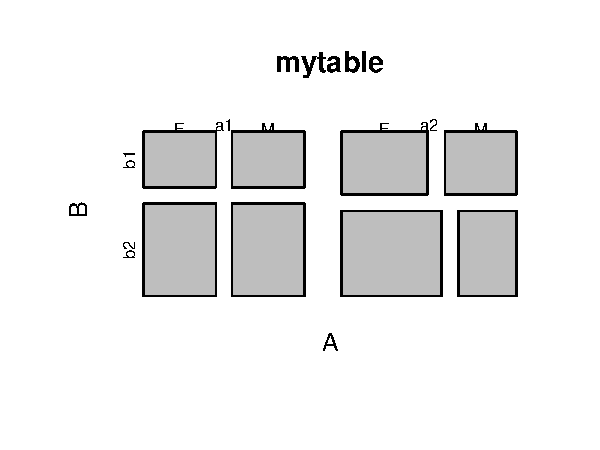
\includegraphics[width=.48\textwidth]{ch02/fig/plot-xtab1} 
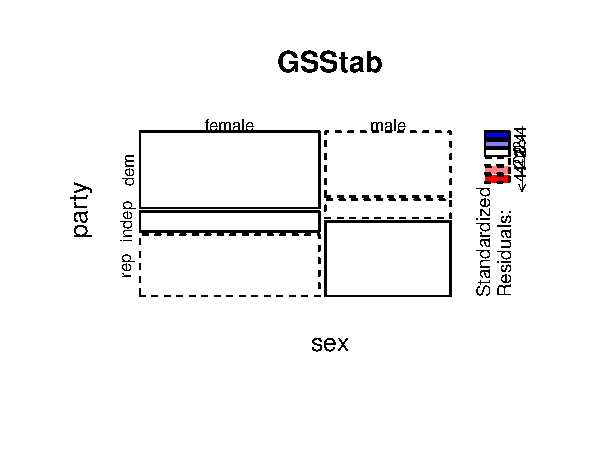
\includegraphics[width=.48\textwidth]{ch02/fig/plot-xtab2} }

\caption[Mosaic plot of tables using the plot method for table objects]{Mosaic plot of tables using the plot method for table objects\label{fig:plot-xtab}}
\end{figure}


\end{knitrout}




\section[Printing tables: structable and ftable]{Printing tables with \func{structable} and \func{ftable}}\label{sec:structable}

For 3-way and larger tables, the functions
\func{ftable} (in the \pkg{stats} package) and
\func{structable} (in \pkg{vcd}) provide a convenient and flexible tabular display in a ``flat'' (2-way) format.

With \code{ftable(X, row.vars=, col.vars=)}, variables assigned to the rows and/or columns of the result
can be specified as the integer numbers or character names of the variables in
the array \code{X}. By default, the last variable is used for the columns.
The formula method, in the form \verb|ftable(colvars ~ rowvars, data)|
allows a formula, where the left and right hand side of formula specify the column and row variables respectively.

\begin{knitrout}
\definecolor{shadecolor}{rgb}{0.969, 0.969, 0.969}\color{fgcolor}\begin{kframe}
\begin{alltt}
 \hlkwd{ftable}\hlstd{(UCB)}                    \hlcom{# default}
\end{alltt}
\begin{verbatim}
##                 Department   A   B   C   D   E   F
## Sex    Admitted                                   
## Male   Yes                 512 353 120 138  53  22
##        No                  313 207 205 279 138 351
## Female Yes                  89  17 202 131  94  24
##        No                   19   8 391 244 299 317
\end{verbatim}
\begin{alltt}
\hlcom{#ftable(UCB, row.vars=1:2)      # same result}
 \hlkwd{ftable}\hlstd{(Admitted} \hlopt{+} \hlstd{Sex} \hlopt{~} \hlstd{Department,} \hlkwc{data}\hlstd{=UCB)}   \hlcom{# formula method}
\end{alltt}
\begin{verbatim}
##            Admitted  Yes          No       
##            Sex      Male Female Male Female
## Department                                 
## A                    512     89  313     19
## B                    353     17  207      8
## C                    120    202  205    391
## D                    138    131  279    244
## E                     53     94  138    299
## F                     22     24  351    317
\end{verbatim}
\end{kframe}
\end{knitrout}


The \func{structable} function is similar, but more general, and uses
recursive splits in the vertical or horizontal directions
(similar to the construction of mosaic displays).  It works with both
data frames and table objects.
\begin{knitrout}
\definecolor{shadecolor}{rgb}{0.969, 0.969, 0.969}\color{fgcolor}\begin{kframe}
\begin{alltt}
\hlkwd{structable}\hlstd{(HairEyeColor)}                   \hlcom{# show the table: default}
\end{alltt}
\begin{verbatim}
##              Eye Brown Blue Hazel Green
## Hair  Sex                              
## Black Male          32   11    10     3
##       Female        36    9     5     2
## Brown Male          53   50    25    15
##       Female        66   34    29    14
## Red   Male          10   10     7     7
##       Female        16    7     7     7
## Blond Male           3   30     5     8
##       Female         4   64     5     8
\end{verbatim}
\begin{alltt}
\hlkwd{structable}\hlstd{(Hair}\hlopt{+}\hlstd{Sex} \hlopt{~} \hlstd{Eye, HairEyeColor)}   \hlcom{# specify col ~ row variables}
\end{alltt}
\begin{verbatim}
##       Hair Black        Brown         Red        Blond       
##       Sex   Male Female  Male Female Male Female  Male Female
## Eye                                                          
## Brown         32     36    53     66   10     16     3      4
## Blue          11      9    50     34   10      7    30     64
## Hazel         10      5    25     29    7      7     5      5
## Green          3      2    15     14    7      7     8      8
\end{verbatim}
\end{kframe}
\end{knitrout}

It also returns an object of class \code{"structable"} for which there are a
variety of special methods.  For example, the transpose function \func{t}
interchanges rows and columns, so that \code{t(structable(HairEyeColor))}
produces the second result shown just above;
\class{structable} objects can be subset using the 
\code{[} and \code{[[} operators, using either level indices or names.
There are also plot methods, so that \func{plot} and \func{mosaic}
produce mosaic plots.
\begin{knitrout}
\definecolor{shadecolor}{rgb}{0.969, 0.969, 0.969}\color{fgcolor}\begin{kframe}
\begin{alltt}
\hlstd{HSE} \hlkwb{<-} \hlkwd{structable}\hlstd{(Hair}\hlopt{+}\hlstd{Sex} \hlopt{~} \hlstd{Eye, HairEyeColor)}   \hlcom{# save structable object}
\hlstd{HSE[}\hlnum{1}\hlopt{:}\hlnum{2}\hlstd{,]}                                         \hlcom{# subset rows}
\end{alltt}
\begin{verbatim}
##       Hair Black        Brown         Red        Blond       
##       Sex   Male Female  Male Female Male Female  Male Female
## Eye                                                          
## Brown         32     36    53     66   10     16     3      4
## Blue          11      9    50     34   10      7    30     64
\end{verbatim}
\begin{alltt}
\hlkwd{mosaic}\hlstd{(HSE,} \hlkwc{shade}\hlstd{=}\hlnum{TRUE}\hlstd{,} \hlkwc{legend}\hlstd{=}\hlnum{FALSE}\hlstd{)}             \hlcom{# plot it}
\end{alltt}
\end{kframe}

\centerline{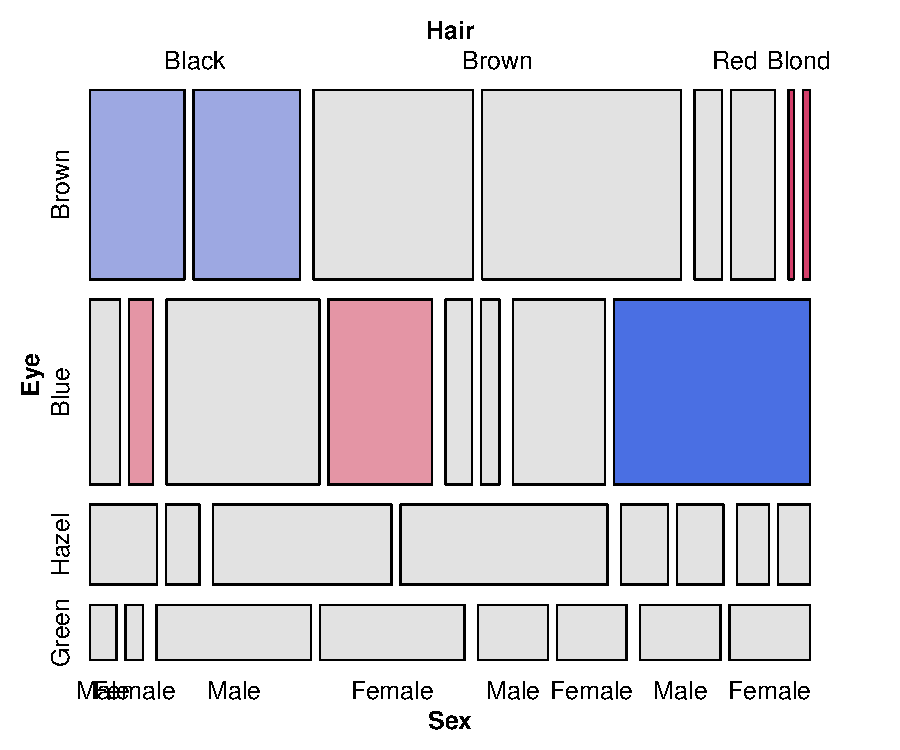
\includegraphics[width=.7\textwidth]{ch02/fig/structable1} }



\end{knitrout}


\subsection{Publishing tables to \LaTeX or HTML}
OK, you've read your data into \R, done some analysis, and now want to
include some tables in a \LaTeX document or in a web page in HTML format.
Formatting tables for these purposes is often tedious and error-prone.

There are a great many packages in \R that provide for nicely formatted,
publishable tables for a wide variety of purposes; indeed, most of the tables
in this book are generated using these tools.
See \citet{Leifeld:2013:JSS} for description of the \Rpackage{texreg}
and a comparison with some of the other packages.

Here, we simply illustrate the \Rpackage{xtable}, which, along with
capabilities for statistical model summaries, time-series data, and
so forth, has a \code{xtable.table} method for one-way and two-way
table objects.

The \data{HorseKicks} data is a small one-way frequency table 
described in \exref{ex:horskick1} and containing the frequencies
of 0, 1, 2, 3, 4 deaths per corps-year by horse-kick among soldiers in 20 corps in
the Prussian army.
\begin{knitrout}
\definecolor{shadecolor}{rgb}{0.969, 0.969, 0.969}\color{fgcolor}\begin{kframe}
\begin{alltt}
\hlkwd{data}\hlstd{(HorseKicks,} \hlkwc{package}\hlstd{=}\hlstr{"vcd"}\hlstd{)}
\hlstd{HorseKicks}
\end{alltt}
\begin{verbatim}
## nDeaths
##   0   1   2   3   4 
## 109  65  22   3   1
\end{verbatim}
\end{kframe}
\end{knitrout}

By default, \func{xtable} formats this in \LaTeX as a vertical table,
and prints the \LaTeX markup to the \R console.  This output is shown
below (without the usual \code{\#\#} comment used to indicate \R output).
\begin{knitrout}
\definecolor{shadecolor}{rgb}{0.969, 0.969, 0.969}\color{fgcolor}\begin{kframe}
\begin{alltt}
\hlkwd{library}\hlstd{(xtable)}
\hlkwd{xtable}\hlstd{(HorseKicks)}
\end{alltt}
\begin{verbatim}
% latex table generated in R 3.0.1 by xtable 1.7-1 package
% Fri Feb 21 16:29:56 2014
\begin{table}[ht]
\centering
\begin{tabular}{rr}
  \hline
 & nDeaths \\ 
  \hline
0 & 109 \\ 
  1 &  65 \\ 
  2 &  22 \\ 
  3 &   3 \\ 
  4 &   1 \\ 
   \hline
\end{tabular}
\end{table}
\end{verbatim}
\end{kframe}
\end{knitrout}

When this is rendered in a \LaTeX document, the result of \func{xtable}
appears as shown in the table below.
\begin{kframe}
\begin{alltt}
\hlkwd{xtable}\hlstd{(HorseKicks)}
\end{alltt}
\end{kframe}% latex table generated in R 3.0.1 by xtable 1.7-1 package
% Fri Feb 21 16:29:56 2014
\begin{table}[ht]
\centering
\begin{tabular}{rr}
  \hline
 & nDeaths \\ 
  \hline
0 & 109 \\ 
  1 &  65 \\ 
  2 &  22 \\ 
  3 &   3 \\ 
  4 &   1 \\ 
   \hline
\end{tabular}
\end{table}



The table above isn't quite right, because the column label ``nDeaths''
belongs to the first column, and the second column should be labeled ``Freq''.
To correct that, we convert the \data{HorseKicks} table to a data frame
(see \secref{sec:convert} for details), add the appropriate \code{colnames},
and use the \code{xtable.print} method to supply some other options.
\begin{kframe}
\begin{alltt}
\hlstd{tab} \hlkwb{<-} \hlkwd{as.data.frame}\hlstd{(HorseKicks)}
\hlkwd{colnames}\hlstd{(tab)} \hlkwb{<-} \hlkwd{c}\hlstd{(}\hlstr{"nDeaths"}\hlstd{,} \hlstr{"Freq"}\hlstd{)}
\hlkwd{print}\hlstd{(}\hlkwd{xtable}\hlstd{(tab),} \hlkwc{include.rownames}\hlstd{=}\hlnum{FALSE}\hlstd{,} \hlkwc{include.colnames}\hlstd{=}\hlnum{TRUE}\hlstd{)}
\end{alltt}
\end{kframe}% latex table generated in R 3.0.1 by xtable 1.7-1 package
% Fri Feb 21 16:29:56 2014
\begin{table}[ht]
\centering
\begin{tabular}{lr}
  \hline
nDeaths & Freq \\ 
  \hline
0 & 109 \\ 
  1 &  65 \\ 
  2 &  22 \\ 
  3 &   3 \\ 
  4 &   1 \\ 
   \hline
\end{tabular}
\end{table}



Finally, in \chref{ch:discrete}, we display a number of similar one-way
frequency tables in a transposed form to save display space.  
\tabref{tab:horsetab} is the finished version we show there. 
The code below uses the following techniques:
(a) \func{addmargins} is used to show the sum of all the frequency values;
(b) \func{t} transposes the data frame to have 2 rows;
(c) \func{rownames} assigns the labels we want for the rows;
(d) using the \code{caption} argument provides a table caption, and a numbered
table in \LaTeX.
(d) column alignment (\code{"r"} or \code{"l"}) for the table columns
is computed as a character string used for the \code{align} argument.
\begin{kframe}
\begin{alltt}
\hlstd{horsetab} \hlkwb{<-} \hlkwd{t}\hlstd{(} \hlkwd{as.data.frame}\hlstd{(} \hlkwd{addmargins}\hlstd{( HorseKicks ) ) )}
\hlkwd{rownames}\hlstd{( horsetab )} \hlkwb{<-} \hlkwd{c}\hlstd{(} \hlstr{"Number of deaths"}\hlstd{,} \hlstr{"Frequency"} \hlstd{)}
\hlstd{horsetab} \hlkwb{<-} \hlkwd{xtable}\hlstd{( horsetab,} \hlkwc{digits} \hlstd{=} \hlnum{0}\hlstd{,}
     \hlkwc{caption} \hlstd{=} \hlstr{"von Bortkiewicz's data on deaths by horse kicks"}\hlstd{,}
     \hlkwc{align} \hlstd{=} \hlkwd{paste0}\hlstd{(}\hlstr{"l|"}\hlstd{,} \hlkwd{paste}\hlstd{(}\hlkwd{rep}\hlstd{(}\hlstr{"r"}\hlstd{,} \hlkwd{ncol}\hlstd{(horsetab)),} \hlkwc{collapse}\hlstd{=}\hlstr{""}\hlstd{))}
     \hlstd{)}
\hlkwd{print}\hlstd{(horsetab,} \hlkwc{include.colnames}\hlstd{=}\hlnum{FALSE}\hlstd{)}
\end{alltt}
\end{kframe}% latex table generated in R 3.0.1 by xtable 1.7-1 package
% Fri Feb 21 16:29:56 2014
\begin{table}[ht]
\centering
\begin{tabular}{l|rrrrrr}
  \hline
  \hline
Number of deaths & 0 & 1 & 2 & 3 & 4 & Sum \\ 
  Frequency & 109 &  65 &  22 &   3 &   1 & 200 \\ 
   \hline
\end{tabular}
\caption{von Bortkiewicz's data on deaths by horse kicks} 
\end{table}




\section[Collapsing over table factors]{Collapsing over table factors: \func{aggregate}, \func{margin.table} and \func{apply}}\label{sec:collapse}

It sometimes happens that we have a data set with more variables or factors than 
we want to analyse, or else, having done some initial analyses, we decide that
certain factors are not important, and so should be excluded from graphic displays
by collapsing (summing) over them.  For example, mosaic plots and fourfold displays
are often simpler to construct from versions of the data collapsed over
the factors which are not shown in the plots.

The appropriate tools to use again depend on
the form in which the data are represented--- a case-form data frame, a
frequency-form data frame (\func{aggregate}), or a table-form array or 
table object (\func{margin.table} or \func{apply}).

When the data are in frequency form, and we want to produce another
frequency data frame, \func{aggregate} is a handy tool, using
the argument \code{FUN=sum} to sum the frequency variable over the 
factors \emph{not} mentioned in the formula.

\begin{Example}[dayton1]{Dayton survey}
The data frame \data{DaytonSurvey} in the \pkg{vcdExtra} package represents a
$2^5$ table giving the frequencies of reported use (``ever used?'') of 
alcohol, cigarettes and marijuana in a sample of 2276 high school seniors,
also classified by sex and race.  

\begin{knitrout}
\definecolor{shadecolor}{rgb}{0.969, 0.969, 0.969}\color{fgcolor}\begin{kframe}
\begin{alltt}
\hlkwd{data}\hlstd{(DaytonSurvey,} \hlkwc{package}\hlstd{=}\hlstr{"vcdExtra"}\hlstd{)}
\hlkwd{str}\hlstd{(DaytonSurvey)}
\end{alltt}
\begin{verbatim}
## 'data.frame':	32 obs. of  6 variables:
##  $ cigarette: Factor w/ 2 levels "Yes","No": 1 2 1 2 1 2 1 2 1 2 ...
##  $ alcohol  : Factor w/ 2 levels "Yes","No": 1 1 2 2 1 1 2 2 1 1 ...
##  $ marijuana: Factor w/ 2 levels "Yes","No": 1 1 1 1 2 2 2 2 1 1 ...
##  $ sex      : Factor w/ 2 levels "female","male": 1 1 1 1 1 1 1 1 2 2 ...
##  $ race     : Factor w/ 2 levels "white","other": 1 1 1 1 1 1 1 1 1 1 ...
##  $ Freq     : num  405 13 1 1 268 218 17 117 453 28 ...
\end{verbatim}
\begin{alltt}
\hlkwd{head}\hlstd{(DaytonSurvey)}
\end{alltt}
\begin{verbatim}
##   cigarette alcohol marijuana    sex  race Freq
## 1       Yes     Yes       Yes female white  405
## 2        No     Yes       Yes female white   13
## 3       Yes      No       Yes female white    1
## 4        No      No       Yes female white    1
## 5       Yes     Yes        No female white  268
## 6        No     Yes        No female white  218
\end{verbatim}
\end{kframe}
\end{knitrout}


To focus on the associations among the
substances, we want to collapse over sex and race. The right-hand side of the formula
used in the call to \func{aggregate} gives the factors to be retained in the
new frequency data frame, \code{Dayton.ACM.df}.  The left-hand side is
the frequency variable (\code{Freq}), and we aggregate using the \code{FUN=sum}.

\begin{knitrout}
\definecolor{shadecolor}{rgb}{0.969, 0.969, 0.969}\color{fgcolor}\begin{kframe}
\begin{alltt}
\hlcom{# data in frequency form: collapse over sex and race}
\hlstd{Dayton.ACM.df} \hlkwb{<-} \hlkwd{aggregate}\hlstd{(Freq} \hlopt{~} \hlstd{cigarette}\hlopt{+}\hlstd{alcohol}\hlopt{+}\hlstd{marijuana,}
                           \hlkwc{data}\hlstd{=DaytonSurvey,} \hlkwc{FUN}\hlstd{=sum)}
\hlstd{Dayton.ACM.df}
\end{alltt}
\begin{verbatim}
##   cigarette alcohol marijuana Freq
## 1       Yes     Yes       Yes  911
## 2        No     Yes       Yes   44
## 3       Yes      No       Yes    3
## 4        No      No       Yes    2
## 5       Yes     Yes        No  538
## 6        No     Yes        No  456
## 7       Yes      No        No   43
## 8        No      No        No  279
\end{verbatim}
\end{kframe}
\end{knitrout}

\end{Example}

When the data are in table form, and we want to produce another
table, \func{apply} with \code{FUN=sum} can be used in a similar way
to sum the table over dimensions not mentioned in the \code{MARGIN}
argument.  \func{margin.table} is just a wrapper for \func{apply}
using the \func{sum} function.


\begin{Example}[dayton2]{Dayton survey}
To illustrate, we first convert the \data{DaytonSurvey} to a 5-way
table using \func{xtabs}, giving \code{Dayton.tab}.  

\begin{knitrout}
\definecolor{shadecolor}{rgb}{0.969, 0.969, 0.969}\color{fgcolor}\begin{kframe}
\begin{alltt}
\hlcom{# convert to table form}
\hlstd{Dayton.tab} \hlkwb{<-} \hlkwd{xtabs}\hlstd{(Freq}\hlopt{~}\hlstd{cigarette}\hlopt{+}\hlstd{alcohol}\hlopt{+}\hlstd{marijuana}\hlopt{+}\hlstd{sex}\hlopt{+}\hlstd{race,}
                    \hlkwc{data}\hlstd{=DaytonSurvey)}
\hlkwd{structable}\hlstd{(cigarette}\hlopt{+}\hlstd{alcohol}\hlopt{+}\hlstd{marijuana} \hlopt{~} \hlstd{sex}\hlopt{+}\hlstd{race,} \hlkwc{data}\hlstd{=Dayton.tab)}
\end{alltt}
\begin{verbatim}
##              cigarette Yes              No            
##              alcohol   Yes      No     Yes      No    
##              marijuana Yes  No Yes  No Yes  No Yes  No
## sex    race                                           
## female white           405 268   1  17  13 218   1 117
##        other            23  23   0   1   2  19   0  12
## male   white           453 228   1  17  28 201   1 133
##        other            30  19   1   8   1  18   0  17
\end{verbatim}
\end{kframe}
\end{knitrout}

Then, use \func{apply} on \code{Dayton.tab} to give the
3-way table \code{Dayton.ACM.tab} summed over sex and race.
The elements in this new table are the column sums for 
\code{Dayton.tab} shown by \func{structable} just above.

\begin{knitrout}
\definecolor{shadecolor}{rgb}{0.969, 0.969, 0.969}\color{fgcolor}\begin{kframe}
\begin{alltt}
\hlcom{# collapse over sex and race}
\hlstd{Dayton.ACM.tab} \hlkwb{<-} \hlkwd{apply}\hlstd{(Dayton.tab,} \hlkwc{MARGIN}\hlstd{=}\hlnum{1}\hlopt{:}\hlnum{3}\hlstd{,} \hlkwc{FUN}\hlstd{=sum)}
\hlstd{Dayton.ACM.tab} \hlkwb{<-} \hlkwd{margin.table}\hlstd{(Dayton.tab,} \hlnum{1}\hlopt{:}\hlnum{3}\hlstd{)}   \hlcom{# same result}
\hlkwd{structable}\hlstd{(cigarette}\hlopt{+}\hlstd{alcohol} \hlopt{~} \hlstd{marijuana,} \hlkwc{data}\hlstd{=Dayton.ACM.tab)}
\end{alltt}
\begin{verbatim}
##           cigarette Yes      No    
##           alcohol   Yes  No Yes  No
## marijuana                          
## Yes                 911   3  44   2
## No                  538  43 456 279
\end{verbatim}
\end{kframe}
\end{knitrout}

\end{Example}

Many of these operations can be performed using the \verb|**ply()| functions
in the \pkg{plyr} package.
For example, with the data in a frequency form data frame, use \func{ddply}
to collapse over unmentioned factors, and \func{plyr::summarise}%
\footnote{
Ugh. This \pkg{plyr} function clashes with a function of the same name in \pkg{vcdExtra}.
In this book I will use the explicit double-colon notation to keep them
separate.
}
as the function to be applied to each piece.
\begin{knitrout}
\definecolor{shadecolor}{rgb}{0.969, 0.969, 0.969}\color{fgcolor}\begin{kframe}
\begin{alltt}
\hlstd{Dayton.ACM.df} \hlkwb{<-} \hlkwd{ddply}\hlstd{(DaytonSurvey,} \hlkwd{.}\hlstd{(cigarette, alcohol, marijuana),}
                       \hlstd{plyr::summarise,} \hlkwc{Freq}\hlstd{=}\hlkwd{sum}\hlstd{(Freq))}
\end{alltt}
\end{kframe}
\end{knitrout}


\subsection[Collapsing table levels]{Collapsing table levels: \func{collapse.table}}

A related problem arises when we have a table or array and for some purpose
we want to reduce the number of levels of some factors by summing subsets
of the frequencies.  For example, we may have initially coded Age in 10-year
intervals, and decide that, either for analysis or display purposes, we
want to reduce Age to 20-year intervals.  The \func{collapse.table} function
in \pkg{vcdExtra} was designed for this purpose.

\begin{Example}[collapse-cat]{Collapsing categories}
Create a 3-way table, and collapse Age from 10-year to 20-year intervals
and Education from three levels to two.
To illustrate, we first generate a $2 \times 6 \times 3$ table of random counts from a 
Poisson distribution with mean of 100, with factors \var{sex}, \var{age}
and \var{education}.
\begin{knitrout}
\definecolor{shadecolor}{rgb}{0.969, 0.969, 0.969}\color{fgcolor}\begin{kframe}
\begin{alltt}
\hlcom{# create some sample data in frequency form}
\hlstd{sex} \hlkwb{<-} \hlkwd{c}\hlstd{(}\hlstr{"Male"}\hlstd{,} \hlstr{"Female"}\hlstd{)}
\hlstd{age} \hlkwb{<-} \hlkwd{c}\hlstd{(}\hlstr{"10-19"}\hlstd{,} \hlstr{"20-29"}\hlstd{,}  \hlstr{"30-39"}\hlstd{,} \hlstr{"40-49"}\hlstd{,} \hlstr{"50-59"}\hlstd{,} \hlstr{"60-69"}\hlstd{)}
\hlstd{education} \hlkwb{<-} \hlkwd{c}\hlstd{(}\hlstr{"low"}\hlstd{,} \hlstr{'med'}\hlstd{,} \hlstr{'high'}\hlstd{)}
\hlstd{dat} \hlkwb{<-} \hlkwd{expand.grid}\hlstd{(}\hlkwc{sex}\hlstd{=sex,} \hlkwc{age}\hlstd{=age,} \hlkwc{education}\hlstd{=education)}
\hlstd{counts} \hlkwb{<-} \hlkwd{rpois}\hlstd{(}\hlnum{36}\hlstd{,} \hlnum{100}\hlstd{)}   \hlcom{# random Possion cell frequencies}
\hlstd{dat} \hlkwb{<-} \hlkwd{cbind}\hlstd{(dat, counts)}
\hlcom{# make it into a 3-way table}
\hlstd{tab1} \hlkwb{<-} \hlkwd{xtabs}\hlstd{(counts} \hlopt{~} \hlstd{sex} \hlopt{+} \hlstd{age} \hlopt{+} \hlstd{education,} \hlkwc{data}\hlstd{=dat)}
\hlkwd{structable}\hlstd{(tab1)}
\end{alltt}
\begin{verbatim}
##                  age 10-19 20-29 30-39 40-49 50-59 60-69
## sex    education                                        
## Male   low              91   110   106    95   107    98
##        med             108   104    97   100   107   112
##        high            104   104   106   101    92    95
## Female low             115   103    96    93   112    94
##        med              96    88    92   103    98    93
##        high             84    93   103    93    95   103
\end{verbatim}
\end{kframe}
\end{knitrout}

Now collapse \code{age} to 20-year intervals, and \code{education}
to 2 levels. In the arguments to \func{collapse.table}, levels of \code{age} and \code{education}
given the same label are summed in the resulting smaller table.
\begin{knitrout}
\definecolor{shadecolor}{rgb}{0.969, 0.969, 0.969}\color{fgcolor}\begin{kframe}
\begin{alltt}
\hlcom{# collapse age to 3 levels, education to 2 levels}
\hlstd{tab2} \hlkwb{<-} \hlkwd{collapse.table}\hlstd{(tab1,}
         \hlkwc{age}\hlstd{=}\hlkwd{c}\hlstd{(}\hlstr{"10-29"}\hlstd{,} \hlstr{"10-29"}\hlstd{,}  \hlstr{"30-49"}\hlstd{,} \hlstr{"30-49"}\hlstd{,} \hlstr{"50-69"}\hlstd{,} \hlstr{"50-69"}\hlstd{),}
         \hlkwc{education}\hlstd{=}\hlkwd{c}\hlstd{(}\hlstr{"<high"}\hlstd{,} \hlstr{"<high"}\hlstd{,} \hlstr{"high"}\hlstd{))}
\hlkwd{structable}\hlstd{(tab2)}
\end{alltt}
\begin{verbatim}
##                  age 10-29 30-49 50-69
## sex    education                      
## Male   <high           413   398   424
##        high            208   207   187
## Female <high           402   384   397
##        high            177   196   198
\end{verbatim}
\end{kframe}
\end{knitrout}

\end{Example}

\section{Converting among frequency tables and data frames}\label{sec:convert}

As we've seen, a given contingency table can be represented 
equivalently in case form, frequency form and table form.
However, some \R functions were designed for one particular representation.
\tabref{tab:convert} shows some handy tools for converting from one form to another.

\begin{table}[htb]
 \caption{Tools for converting among different forms for categorical data}\label{tab:convert}
 \newsavebox{\adfxtabs}
 \savebox{\adfxtabs}{\begin{tabular}{ll} \code{Z <- xtabs(~A+B)} \\ \code{as.data.frame(Z)} \\ \end{tabular}}
 \begin{center}
   \begin{tabular}{l|lll}
  \hline
                 & \multicolumn{3}{c}{\textbf{To this}} \\
	\textbf{From this}      &     Case form         & Frequency form             &  Table form \\
	\hline
  Case form      &                        & \usebox{\adfxtabs}        &  \verb|table(A,B)|  \\ 
%	Case form      &                        & {\small\verb|as.data.frame(xtabs(~A+B))|}        &  \verb|table(A,B)|  \\ 
	Frequency form &  \verb|expand.dft(X)|  &                           & \verb|xtabs(count~A+B)|\\
	Table form     &  \verb|expand.dft(X)|  & \verb|as.data.frame(X)|   &       \\
	\hline
   \end{tabular}
 \end{center}
\end{table}

\subsection{Table form to frequency form}
A contingency table in table form (an object of class \class{table}) can be converted
to a data frame in frequency form with \func{as.data.frame}.%
\footnote{
Because \R is object-oriented, this is actually a short-hand for
the function \func{as.data.frame.table}.
}  
The resulting
data frame contains columns
representing the classifying factors and the table entries (as a column named by
the \code{responseName} argument, defaulting to \code{Freq}.  The function
\func{as.data.frame} is the inverse of \func{xtabs}, which converts a data frame to a table.

\begin{Example}[GSS-convert]{General social survey}
Convert the \code{GSStab} in table form to a data.frame in frequency form.
By default, the frequency variable is named \code{Freq}, and the variables
\code{sex} and \code{party} are made factors.
\begin{knitrout}
\definecolor{shadecolor}{rgb}{0.969, 0.969, 0.969}\color{fgcolor}\begin{kframe}
\begin{alltt}
\hlkwd{as.data.frame}\hlstd{(GSStab)}
\end{alltt}
\begin{verbatim}
##      sex party Freq
## 1 female   dem  279
## 2   male   dem  165
## 3 female indep   73
## 4   male indep   47
## 5 female   rep  225
## 6   male   rep  191
\end{verbatim}
\end{kframe}
\end{knitrout}

\end{Example}

In addition, there are situations where numeric table variables are represented as
factors, but you need to
convert them to numerics for calculation purposes.

\begin{Example}[horse.df]{Horse kicks data}

For example, We might want to calculate the weighted mean of \code{nDeaths}
in the \data{HorseKicks} data. 
Using \func{as.data.frame} won't work here, because the variable \code{nDeaths}
becomes a factor.

\begin{knitrout}
\definecolor{shadecolor}{rgb}{0.969, 0.969, 0.969}\color{fgcolor}\begin{kframe}
\begin{alltt}
\hlkwd{str}\hlstd{(}\hlkwd{as.data.frame}\hlstd{(HorseKicks))}
\end{alltt}
\begin{verbatim}
## 'data.frame':	5 obs. of  2 variables:
##  $ nDeaths: Factor w/ 5 levels "0","1","2","3",..: 1 2 3 4 5
##  $ Freq   : int  109 65 22 3 1
\end{verbatim}
\end{kframe}
\end{knitrout}

One solution is to use \func{data.frame} directly and \func{as.numeric}
to coerce the table names to numbers.
\begin{knitrout}
\definecolor{shadecolor}{rgb}{0.969, 0.969, 0.969}\color{fgcolor}\begin{kframe}
\begin{alltt}
\hlstd{horse.df} \hlkwb{<-} \hlkwd{data.frame}\hlstd{(}\hlkwc{nDeaths} \hlstd{=} \hlkwd{as.numeric}\hlstd{(}\hlkwd{names}\hlstd{(HorseKicks)),}
                       \hlkwc{Freq} \hlstd{=} \hlkwd{as.vector}\hlstd{(HorseKicks))}
\hlkwd{str}\hlstd{(horse.df)}
\end{alltt}
\begin{verbatim}
## 'data.frame':	5 obs. of  2 variables:
##  $ nDeaths: num  0 1 2 3 4
##  $ Freq   : int  109 65 22 3 1
\end{verbatim}
\begin{alltt}
\hlstd{horse.df}
\end{alltt}
\begin{verbatim}
##   nDeaths Freq
## 1       0  109
## 2       1   65
## 3       2   22
## 4       3    3
## 5       4    1
\end{verbatim}
\end{kframe}
\end{knitrout}

Then, \func{weighted.mean} works as we would like:
\begin{knitrout}
\definecolor{shadecolor}{rgb}{0.969, 0.969, 0.969}\color{fgcolor}\begin{kframe}
\begin{alltt}
\hlkwd{weighted.mean}\hlstd{(horse.df}\hlopt{$}\hlstd{nDeaths,} \hlkwc{weights}\hlstd{=horse.df}\hlopt{$}\hlstd{Freq)}
\end{alltt}
\begin{verbatim}
## [1] 2
\end{verbatim}
\end{kframe}
\end{knitrout}

\end{Example}

\subsection{Case form to table form}
Going the other way, we use \func{table} to convert from case form to table form.

\begin{Example}[Arth-convert]{Arthritis treatment}
Convert the \code{Arthritis} data in case form to a 3-way table of
\code{Treatment} $\times$ \code{Sex} $\times$ \code{Improved}.
We select the desired columns with their names, but could also use column
numbers, e.g., \code{table(Arthritis[,c(2,3,5)])}.
%Note the use of \func{with} to avoid having to use \code{Arthritis\$Treatment} etc. within %the call to \func{table}.%
\begin{knitrout}
\definecolor{shadecolor}{rgb}{0.969, 0.969, 0.969}\color{fgcolor}\begin{kframe}
\begin{alltt}
\hlstd{Art.tab} \hlkwb{<-} \hlkwd{table}\hlstd{(Arthritis[,}\hlkwd{c}\hlstd{(}\hlstr{"Treatment"}\hlstd{,} \hlstr{"Sex"}\hlstd{,} \hlstr{"Improved"}\hlstd{)])}
\hlkwd{str}\hlstd{(Art.tab)}
\end{alltt}
\begin{verbatim}
##  'table' int [1:2, 1:2, 1:3] 19 6 10 7 7 5 0 2 6 16 ...
##  - attr(*, "dimnames")=List of 3
##   ..$ Treatment: chr [1:2] "Placebo" "Treated"
##   ..$ Sex      : chr [1:2] "Female" "Male"
##   ..$ Improved : chr [1:3] "None" "Some" "Marked"
\end{verbatim}
\begin{alltt}
\hlkwd{ftable}\hlstd{(Art.tab)}
\end{alltt}
\begin{verbatim}
##                  Improved None Some Marked
## Treatment Sex                             
## Placebo   Female            19    7      6
##           Male              10    0      1
## Treated   Female             6    5     16
##           Male               7    2      5
\end{verbatim}
\end{kframe}
\end{knitrout}

\end{Example}

\subsection{Table form to case form}
There may also be times that you will need an equivalent case form data frame
with factors  representing the table variables
rather than the frequency  table.
For example, the \func{mca} function in package \pkg{MASS}
only operates on data in this format. 
The function \func{expand.dft}%
\footnote{
The original code for this function was provided by Marc Schwarz on the R-Help
mailing list.
}
in \pkg{vcdExtra}
does this, converting a table into a case form.

\begin{Example}[Arth-convert2]{Arthritis treatment}
Convert the \data{Arthritis} data in table form (\code{Art.tab}) back to a \code{data.frame}
in case form, with factors
\code{Treatment}, \code{Sex} and \code{Improved}.
\begin{knitrout}
\definecolor{shadecolor}{rgb}{0.969, 0.969, 0.969}\color{fgcolor}\begin{kframe}
\begin{alltt}
\hlstd{Art.df} \hlkwb{<-} \hlkwd{expand.dft}\hlstd{(Art.tab)}
\hlkwd{str}\hlstd{(Art.df)}
\end{alltt}
\begin{verbatim}
## 'data.frame':	84 obs. of  3 variables:
##  $ Treatment: Factor w/ 2 levels "Placebo","Treated": 1 1 1 1 1 1 1 1 1 1 ...
##  $ Sex      : Factor w/ 2 levels "Female","Male": 1 1 1 1 1 1 1 1 1 1 ...
##  $ Improved : Factor w/ 3 levels "Marked","None",..: 2 2 2 2 2 2 2 2 2 2 ...
\end{verbatim}
\end{kframe}
\end{knitrout}

\end{Example}


\section{A complex example}

If you've followed so far, congratulations! You're ready for a more complicated example
that puts together a variety of the skills developed in this chapter:
\begin{seriate}
  \item reading raw data, 
  \item creating tables, 
  \item assigning level names to factors and
  \item collapsing levels or variables for use in analysis.
\end{seriate}

For illustration of these steps, 
we use the dataset \code{tv.dat}, supplied with
the initial implementation of 
mosaic displays in \R by Jay Emerson. 
In turn, they were derived from an early, compelling example of mosaic displays 
\citep{HartiganKleiner:84},
that illustrated the method with data on a large sample of TV viewers
whose behavior had been recorded for the Neilson ratings.
This data set contains sample television audience data from Neilsen
Media Research for the week starting November 6, 1995.


The data file, \code{tv.dat} is stored in frequency form 
as a file with 825 rows and 5 columns.  There is no header line
in the file, so when we use \func{read.table} below, the variables
will be named \code{V1} -- \code{V5}.  This data represents
 a 4-way table of size
$5 \times 11 \times 5 \times 3 = 825$ where the table variables
are \code{V1} -- \code{V4}, and the cell frequency is read
as \code{V5}. 

%% should use \begin{description} ... here
\begin{flushleft}
The table variables are:\\
~~~\code{V1}-- values 1:5 correspond to the days Monday--Friday;\\
~~~\code{V2}-- values 1:11 correspond to the quarter hour times 8:00PM through 10:30PM;\\
~~~\code{V3}-- values 1:5 correspond to ABC, CBS, NBC, Fox, and non-network choices;\\
~~~\code{V4}-- values 1:3 correspond to transition states: turn the television Off, Switch channels,  or Persist in viewing the current channel.
\end{flushleft}

\subsection{Creating data frames and arrays}
The file \code{tv.dat} is stored in the \code{doc/extdata} directory
of \pkg{vcdExtra}; it can be read as follows:
\begin{knitrout}
\definecolor{shadecolor}{rgb}{0.969, 0.969, 0.969}\color{fgcolor}\begin{kframe}
\begin{alltt}
\hlstd{tv.data}\hlkwb{<-}\hlkwd{read.table}\hlstd{(}\hlkwd{system.file}\hlstd{(}\hlstr{"doc"}\hlstd{,}\hlstr{"extdata"}\hlstd{,}\hlstr{"tv.dat"}\hlstd{,}\hlkwc{package}\hlstd{=}\hlstr{"vcdExtra"}\hlstd{))}
\hlkwd{str}\hlstd{(tv.data)}
\end{alltt}
\begin{verbatim}
## 'data.frame':	825 obs. of  5 variables:
##  $ V1: int  1 2 3 4 5 1 2 3 4 5 ...
##  $ V2: int  1 1 1 1 1 2 2 2 2 2 ...
##  $ V3: int  1 1 1 1 1 1 1 1 1 1 ...
##  $ V4: int  1 1 1 1 1 1 1 1 1 1 ...
##  $ V5: int  6 18 6 2 11 6 29 25 17 29 ...
\end{verbatim}
\begin{alltt}
\hlkwd{head}\hlstd{(tv.data,}\hlnum{5}\hlstd{)}
\end{alltt}
\begin{verbatim}
##   V1 V2 V3 V4 V5
## 1  1  1  1  1  6
## 2  2  1  1  1 18
## 3  3  1  1  1  6
## 4  4  1  1  1  2
## 5  5  1  1  1 11
\end{verbatim}
\end{kframe}
\end{knitrout}

To read such data from a local file, just use \func{read.table} in this form:
\begin{knitrout}
\definecolor{shadecolor}{rgb}{0.969, 0.969, 0.969}\color{fgcolor}\begin{kframe}
\begin{alltt}
\hlstd{tv.data}\hlkwb{<-}\hlkwd{read.table}\hlstd{(}\hlstr{"C:/R/data/tv.dat"}\hlstd{)}
\end{alltt}
\end{kframe}
\end{knitrout}


We could use this data in frequency form for analysis by renaming the variables,
and converting the integer-coded factors \code{V1} -- \code{V4} to \R factors.
The lines below use the function \func{within} to avoid having to use
\verb|TV.dat$Day <- factor(TV.dat$Day)| etc., and only supplies labels for the
first variable.
\begin{knitrout}\footnotesize
\definecolor{shadecolor}{rgb}{0.969, 0.969, 0.969}\color{fgcolor}\begin{kframe}
\begin{alltt}
\hlstd{TV.df} \hlkwb{<-} \hlstd{tv.data}
\hlkwd{colnames}\hlstd{(TV.df)} \hlkwb{<-} \hlkwd{c}\hlstd{(}\hlstr{"Day"}\hlstd{,} \hlstr{"Time"}\hlstd{,} \hlstr{"Network"}\hlstd{,} \hlstr{"State"}\hlstd{,} \hlstr{"Freq"}\hlstd{)}
\hlstd{TV.df} \hlkwb{<-} \hlkwd{within}\hlstd{(TV.df, \{Day} \hlkwb{<-} \hlkwd{factor}\hlstd{(Day,}
                                      \hlkwc{labels}\hlstd{=}\hlkwd{c}\hlstd{(}\hlstr{"Mon"}\hlstd{,} \hlstr{"Tue"}\hlstd{,} \hlstr{"Wed"}\hlstd{,} \hlstr{"Thu"}\hlstd{,} \hlstr{"Fri"}\hlstd{))}
                        \hlstd{Time} \hlkwb{<-} \hlkwd{factor}\hlstd{(Time)}
                        \hlstd{Network} \hlkwb{<-} \hlkwd{factor}\hlstd{(Network)}
                        \hlstd{State} \hlkwb{<-} \hlkwd{factor}\hlstd{(State)\})}
\end{alltt}
\end{kframe}
\end{knitrout}


Alternatively, we could just reshape the frequency column 
(\code{V5} or \code{tv.data[,5]}) into
a 4-way array.
In the lines below, we rely on the facts that the
(a) the table is complete--- there are no missing cells,
so \code{nrow(tv.data)}=825;
(b) the observations are ordered so that \code{V1} varies most rapidly and
\code{V4} most slowly.  From this, we can just extract the frequency column
and reshape it into an array using the \code{dim} argument.
The level names are assigned to \code{dimnames(TV)}
and the variable names to \code{names(dimnames(TV))}.
\begin{knitrout}
\definecolor{shadecolor}{rgb}{0.969, 0.969, 0.969}\color{fgcolor}\begin{kframe}
\begin{alltt}
\hlstd{TV} \hlkwb{<-} \hlkwd{array}\hlstd{(tv.data[,}\hlnum{5}\hlstd{],} \hlkwc{dim}\hlstd{=}\hlkwd{c}\hlstd{(}\hlnum{5}\hlstd{,}\hlnum{11}\hlstd{,}\hlnum{5}\hlstd{,}\hlnum{3}\hlstd{))}
\hlkwd{dimnames}\hlstd{(TV)} \hlkwb{<-} \hlkwd{list}\hlstd{(}\hlkwd{c}\hlstd{(}\hlstr{"Mon"}\hlstd{,}\hlstr{"Tue"}\hlstd{,}\hlstr{"Wed"}\hlstd{,}\hlstr{"Thu"}\hlstd{,}\hlstr{"Fri"}\hlstd{),}
                \hlkwd{c}\hlstd{(}\hlstr{"8:00"}\hlstd{,}\hlstr{"8:15"}\hlstd{,}\hlstr{"8:30"}\hlstd{,}\hlstr{"8:45"}\hlstd{,}\hlstr{"9:00"}\hlstd{,}\hlstr{"9:15"}\hlstd{,}\hlstr{"9:30"}\hlstd{,}
                  \hlstr{"9:45"}\hlstd{,}\hlstr{"10:00"}\hlstd{,}\hlstr{"10:15"}\hlstd{,}\hlstr{"10:30"}\hlstd{),}
                \hlkwd{c}\hlstd{(}\hlstr{"ABC"}\hlstd{,}\hlstr{"CBS"}\hlstd{,}\hlstr{"NBC"}\hlstd{,}\hlstr{"Fox"}\hlstd{,}\hlstr{"Other"}\hlstd{),}
                \hlkwd{c}\hlstd{(}\hlstr{"Off"}\hlstd{,}\hlstr{"Switch"}\hlstd{,}\hlstr{"Persist"}\hlstd{))}
\hlkwd{names}\hlstd{(}\hlkwd{dimnames}\hlstd{(TV))}\hlkwb{<-}\hlkwd{c}\hlstd{(}\hlstr{"Day"}\hlstd{,} \hlstr{"Time"}\hlstd{,} \hlstr{"Network"}\hlstd{,} \hlstr{"State"}\hlstd{)}
\end{alltt}
\end{kframe}
\end{knitrout}


More generally (even if there are missing cells), we can 
use \func{xtabs} (or \func{plyr::daply})
to do the cross-tabulation, using \code{V5} as the
frequency variable.  Here's how to do this same operation with \func{xtabs}:
\begin{knitrout}
\definecolor{shadecolor}{rgb}{0.969, 0.969, 0.969}\color{fgcolor}\begin{kframe}
\begin{alltt}
\hlstd{TV} \hlkwb{<-} \hlkwd{xtabs}\hlstd{(V5} \hlopt{~} \hlstd{.,} \hlkwc{data}\hlstd{=tv.data)}
\hlkwd{dimnames}\hlstd{(TV)} \hlkwb{<-} \hlkwd{list}\hlstd{(}\hlkwc{Day}\hlstd{=}\hlkwd{c}\hlstd{(}\hlstr{"Mon"}\hlstd{,}\hlstr{"Tue"}\hlstd{,}\hlstr{"Wed"}\hlstd{,}\hlstr{"Thu"}\hlstd{,}\hlstr{"Fri"}\hlstd{),}
                \hlkwc{Time}\hlstd{=}\hlkwd{c}\hlstd{(}\hlstr{"8:00"}\hlstd{,}\hlstr{"8:15"}\hlstd{,}\hlstr{"8:30"}\hlstd{,}\hlstr{"8:45"}\hlstd{,}\hlstr{"9:00"}\hlstd{,}\hlstr{"9:15"}\hlstd{,}\hlstr{"9:30"}\hlstd{,}
                       \hlstr{"9:45"}\hlstd{,}\hlstr{"10:00"}\hlstd{,}\hlstr{"10:15"}\hlstd{,}\hlstr{"10:30"}\hlstd{),}
                \hlkwc{Network}\hlstd{=}\hlkwd{c}\hlstd{(}\hlstr{"ABC"}\hlstd{,}\hlstr{"CBS"}\hlstd{,}\hlstr{"NBC"}\hlstd{,}\hlstr{"Fox"}\hlstd{,}\hlstr{"Other"}\hlstd{),}
                \hlkwc{State}\hlstd{=}\hlkwd{c}\hlstd{(}\hlstr{"Off"}\hlstd{,}\hlstr{"Switch"}\hlstd{,}\hlstr{"Persist"}\hlstd{))}
\end{alltt}
\end{kframe}
\end{knitrout}

\noindent Note that in the lines above, the variable names are assigned directly
as the names of the elements in the \code{dimnames} list.

\subsection{Subsetting and collapsing}
For many purposes, 
the 4-way table \code{TV}
is too large and awkward to work with. Among the networks,
Fox and Other occur infrequently, so we will remove them.
We can also cut it down to a 3-way table by considering only viewers who persist
with the current station.%
\footnote{This relies on the fact that that indexing
an array drops dimensions of length 1 by default,
using the argument \code{drop=TRUE};
the result is coerced to the lowest possible dimension.
}

\begin{knitrout}\footnotesize
\definecolor{shadecolor}{rgb}{0.969, 0.969, 0.969}\color{fgcolor}\begin{kframe}
\begin{alltt}
\hlstd{TV} \hlkwb{<-} \hlstd{TV[,,}\hlnum{1}\hlopt{:}\hlnum{3}\hlstd{,]}     \hlcom{# keep only ABC, CBS, NBC}
\hlstd{TV} \hlkwb{<-} \hlstd{TV[,,,}\hlnum{3}\hlstd{]}       \hlcom{# keep only Persist -- now a 3 way table}
\hlkwd{structable}\hlstd{(TV)}
\end{alltt}
\begin{verbatim}
##             Time 8:00 8:15 8:30 8:45 9:00 9:15 9:30 9:45 10:00 10:15 10:30
## Day Network                                                               
## Mon ABC           146  151  156   83  325  350  386  340   352   280   278
##     CBS           337  293  304  233  311  251  241  164   252   265   272
##     NBC           263  219  236  140  226  235  239  246   279   263   283
## Tue ABC           244  181  231  205  385  283  345  192   329   351   364
##     CBS           173  180  184  109  218  235  256  250   274   263   261
##     NBC           315  254  280  241  370  214  195  111   188   190   210
## Wed ABC           233  161  194  156  339  264  279  140   237   228   203
##     CBS           158  126  207   59   98  103  122   86   109   105   110
##     NBC           134  146  166   66  194  230  264  143   274   289   306
## Thu ABC           174  183  197  181  187  198  211   86   110   122   117
##     CBS           196  185  195  104  106  116  116   47   102    84    84
##     NBC           515  463  472  477  590  473  446  349   649   705   747
## Fri ABC           294  281  305  239  278  246  245  138   246   232   233
##     CBS           130  144  154   81  129  153  136  126   138   136   152
##     NBC           195  220  248  160  172  164  169   85   183   198   204
\end{verbatim}
\end{kframe}
\end{knitrout}


Finally, for some purposes, we might also want to collapse the 11 times into a smaller number.
Here, we use \func{as.data.frame.table} to convert the table back to a data frame,
 \func{levels} to re-assign the values of \code{Time},
 and finally, \func{xtabs} to give a new, collapsed frequency table.

\begin{knitrout}
\definecolor{shadecolor}{rgb}{0.969, 0.969, 0.969}\color{fgcolor}\begin{kframe}
\begin{alltt}
\hlstd{TV.df} \hlkwb{<-} \hlkwd{as.data.frame.table}\hlstd{(TV)}
\hlkwd{levels}\hlstd{(TV.df}\hlopt{$}\hlstd{Time)} \hlkwb{<-} \hlkwd{c}\hlstd{(}\hlkwd{rep}\hlstd{(}\hlstr{"8:00-8:59"}\hlstd{,}\hlnum{4}\hlstd{),}
                        \hlkwd{rep}\hlstd{(}\hlstr{"9:00-9:59"}\hlstd{,}\hlnum{4}\hlstd{),} \hlkwd{rep}\hlstd{(}\hlstr{"10:00-10:44"}\hlstd{,}\hlnum{3}\hlstd{))}
\hlstd{TV2} \hlkwb{<-} \hlkwd{xtabs}\hlstd{(Freq} \hlopt{~} \hlstd{Day} \hlopt{+} \hlstd{Time} \hlopt{+} \hlstd{Network, TV.df)}
\hlkwd{structable}\hlstd{(Day} \hlopt{~} \hlstd{Time}\hlopt{+}\hlstd{Network,TV2)}
\end{alltt}
\begin{verbatim}
##                     Day  Mon  Tue  Wed  Thu  Fri
## Time        Network                             
## 8:00-8:59   ABC          536  861  744  735 1119
##             CBS         1167  646  550  680  509
##             NBC          858 1090  512 1927  823
## 9:00-9:59   ABC         1401 1205 1022  682  907
##             CBS          967  959  409  385  544
##             NBC          946  890  831 1858  590
## 10:00-10:44 ABC          910 1044  668  349  711
##             CBS          789  798  324  270  426
##             NBC          825  588  869 2101  585
\end{verbatim}
\end{kframe}
\end{knitrout}

Congratulations! If you followed the operations described above,
you are ready for the material described in the rest of the book.
If not, try working through some of exercises below.

As a final step and a prelude to what follows, we construct a mosaic
plot, below (\figref{fig:TV-mosaic}) that focuses on the associations
between the combinations of \code{Day} and \code{Time} and the
\code{Network} viewed.  In terms of a \loglin model, this is
represented by the model formula \verb|~Day:Time + Network|,
which asserts that \code{Network} is independent of the
\code{Day:Time} combinations.

\begin{knitrout}
\definecolor{shadecolor}{rgb}{0.969, 0.969, 0.969}\color{fgcolor}\begin{kframe}
\begin{alltt}
\hlkwd{dimnames}\hlstd{(TV2)}\hlopt{$}\hlstd{Time} \hlkwb{<-} \hlkwd{c}\hlstd{(}\hlstr{"8"}\hlstd{,} \hlstr{"9"}\hlstd{,} \hlstr{"10"}\hlstd{)}     \hlcom{# re-level for mosaic display}
\hlkwd{mosaic}\hlstd{(}\hlopt{~} \hlstd{Day} \hlopt{+} \hlstd{Network} \hlopt{+} \hlstd{Time,} \hlkwc{data}\hlstd{=TV2,} \hlkwc{expected}\hlstd{=}\hlopt{~}\hlstd{Day}\hlopt{:}\hlstd{Time} \hlopt{+} \hlstd{Network,}
         \hlkwc{legend}\hlstd{=}\hlnum{FALSE}\hlstd{,} \hlkwc{gp}\hlstd{=shading_Friendly)}
\end{alltt}
\end{kframe}\begin{figure}[!htb]


\centerline{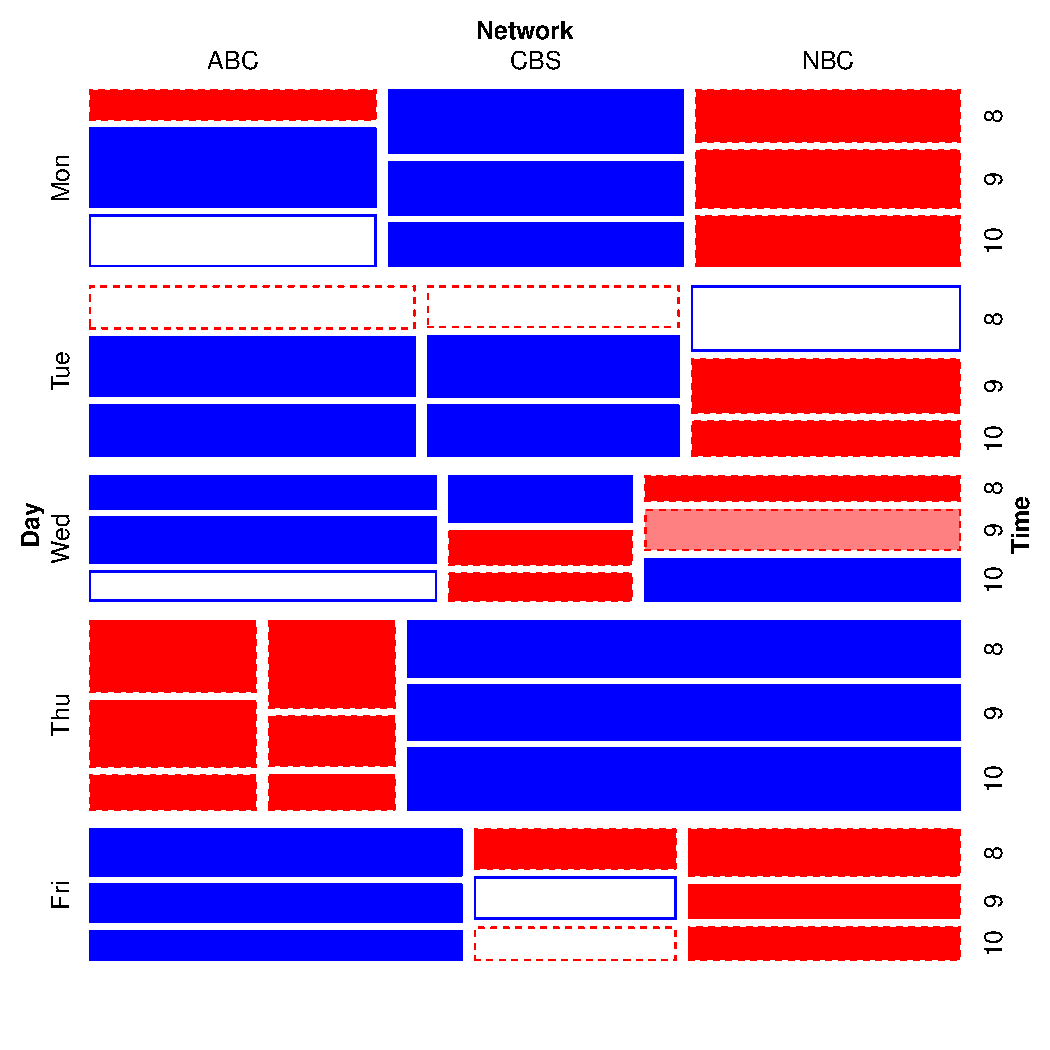
\includegraphics[width=.75\textwidth]{ch02/fig/TV-mosaic} }

\caption[Mosaic plot for the TV data]{Mosaic plot for the TV data showing model of joint independence, \texttt{Day:Time + Network}\label{fig:TV-mosaic}}
\end{figure}


\end{knitrout}

\noindent
The cells shaded in blue show positive associations (observed frequency $>$ expected) and red shows negative associations.  From this it is easy to read 
how network choice varies with day and
time. For example, CBS dominates in all time slots on Monday;
ABC and NBC dominate on Tuesday, particularly in the later time slots;
Thursday is an NBC day, while on Friday, ABC gets the greatest share.

\section{Further reading}\label{sec:ch02-reading}

If you're new to the \R language but keen to get started with linear modeling or logistic regression in the language, take a look at this \emph{Introduction to R},
\url{http://data.princeton.edu/R/introducingR.pdf},
by Germ\'an Rodríguez.

\section{Lab exercises}\label{sec:ch02-exercises}

\begin{enumerate}

\item The packages \pkg{vcd} and \pkg{vcdExtra} contain many data sets with some
examples of analysis and graphical display.  The goal of this exercise is to
familiarize yourself with these resources.

You can get a brief summary of
these using the function \func{datasets}.  Use the following to get a list of
these with some characteristics and titles.
\begin{knitrout}\footnotesize
\definecolor{shadecolor}{rgb}{0.969, 0.969, 0.969}\color{fgcolor}\begin{kframe}
\begin{alltt}
\hlstd{ds} \hlkwb{<-} \hlkwd{datasets}\hlstd{(}\hlkwc{package}\hlstd{=}\hlkwd{c}\hlstd{(}\hlstr{"vcd"}\hlstd{,} \hlstr{"vcdExtra"}\hlstd{))}
\hlkwd{str}\hlstd{(ds)}
\end{alltt}
\begin{verbatim}
## 'data.frame':	65 obs. of  5 variables:
##  $ Package: chr  "vcd" "vcd" "vcd" "vcd" ...
##  $ Item   : chr  "Arthritis" "Baseball" "BrokenMarriage" "Bundesliga" ...
##  $ class  : chr  "data.frame" "data.frame" "data.frame" "data.frame" ...
##  $ dim    : chr  "84x5" "322x25" "20x4" "14018x7" ...
##  $ Title  : chr  "Arthritis Treatment Data" "Baseball Data" "Broken Marriage Data" "Ergebnisse der Fussball-Bundesliga" ...
\end{verbatim}
\end{kframe}
\end{knitrout}

  \begin{enumerate*}
    \item How many data sets are there altogether?  How many are there in each package?
    \item Make a tabular display of the frequencies by \code{Package} and \code{class}.
    \item Choose one or two data sets from this list, and examine their help files
    (e.g., \code{help(Arthritis)} or \code{?Arthritis}).  You can use, e.g.,
    \code{example(Arthritis)} to run the \R code for a given example.
  \end{enumerate*}

\item The data set \data{UCBADdmissions} is a 3-way table of frequencies
classified by \var{Admit}, \var{Gender} and \var{Dept}.
  \begin{enumerate*}
    \item Find the total number of cases contained in this table.
    \item For each department, find the total number of applicants.
    \item For each department, find the overall proportion of applicants who were admitted.
    \item Construct a tabular display of department (rows) and gender (columns), showing
    the proportion of applicants in each cell who were admitted.
  \end{enumerate*}

\item The data set \data{DanishWelfare} in \pkg{vcd}
gives a 4-way, $3 \times 4 \times 3 \times 5$ 
table as a data frame in
frequency form, containing the variable \var{Freq} and four factors,
\var{Alcohol},
\var{Income},
\var{Status} and
\var{Urban}.  The variable \var{Alcohol} can be considered as the
response variable, and the others as possible predictors.

  \begin{enumerate*}
    \item Find the total number of cases represented in this table.
    \item In this form, the variables \var{Alcohol} and \var{Income}
    should arguably be considered \emph{ordered} factors.  Change them
    to make them ordered.
    \item Convert this data frame to table form, \code{DanishWelfare.tab},
    a 4-way array containing the
    frequencies with appropriate variable names and level names.
    \item The variable \var{Urban} has 5 categories.  Find the total frequencies
    in each of these.  How would you collapse the table to have have only
    two categories, \code{City}, \code{Non-city}?
    \item Use \func{structable} or \func{ftable} to produce a pleasing
    flattened display of the frequencies in the 4-way table.  Choose the
    variables used as row and column variables to make it easier to compare
    levels of \var{Alcohol} across the other factors.
  \end{enumerate*}

\item The data set \data{UKSoccer} in \pkg{vcd} gives the distributions of
number of goals scored by the 20 teams in the  1995/96 season of the
Premier League of the UK Football Association.  
\begin{knitrout}
\definecolor{shadecolor}{rgb}{0.969, 0.969, 0.969}\color{fgcolor}\begin{kframe}
\begin{alltt}
\hlkwd{data}\hlstd{(UKSoccer,} \hlkwc{package}\hlstd{=}\hlstr{"vcd"}\hlstd{)}
\hlkwd{ftable}\hlstd{(UKSoccer)}
\end{alltt}
\begin{verbatim}
##      Away  0  1  2  3  4
## Home                    
## 0         27 29 10  8  2
## 1         59 53 14 12  4
## 2         28 32 14 12  4
## 3         19 14  7  4  1
## 4          7  8 10  2  0
\end{verbatim}
\end{kframe}
\end{knitrout}

This two-way table classifies all $20 \times 19 = 380$ games by the joint
outcome (Home, Away), the number of goals scored by the \code{Home} and 
\code{Away} teams.
The value \code{4} in this table actually represents 4 or more goals.

  \begin{enumerate*}
    \item Verify that the total number of games represented in this table is 380.
    \item Find the marginal total of the number of goals scored by each of
    the home and away teams. 
    \item Express each of the marginal totals as proportions.  
    \item Comment on the distribution of the numbers of home-team and away-team
    goals.  Is there any evidence that home teams score more goals on average?

  \end{enumerate*}

\item The one-way frequency table, \data{Saxony} in \pkg{vcd} records the frequencies
of families with 0, 1, 2, $\dots$ 12 male children, among 6115 families with 12
children.  This data set is used extensively in \chref{ch:discrete}.
\begin{knitrout}
\definecolor{shadecolor}{rgb}{0.969, 0.969, 0.969}\color{fgcolor}\begin{kframe}
\begin{alltt}
\hlkwd{data}\hlstd{(Saxony,} \hlkwc{package}\hlstd{=}\hlstr{"vcd"}\hlstd{)}
\hlstd{Saxony}
\end{alltt}
\begin{verbatim}
## nMales
##    0    1    2    3    4    5    6    7    8    9   10   11 
##    3   24  104  286  670 1033 1343 1112  829  478  181   45 
##   12 
##    7
\end{verbatim}
\end{kframe}
\end{knitrout}

Another data set, \data{Geissler} in the \Rpackage{vcdExtra}, gives the complete
tabulation of all combinations of \code{boys} and \code{girls} in families with
a given total number of children \code{size}.  The task here is to create an
equivalent table, \code{Saxony12} from the \data{Geissler} data.
\begin{knitrout}
\definecolor{shadecolor}{rgb}{0.969, 0.969, 0.969}\color{fgcolor}\begin{kframe}
\begin{alltt}
\hlkwd{data}\hlstd{(Geissler,} \hlkwc{package}\hlstd{=}\hlstr{"vcdExtra"}\hlstd{)}
\hlkwd{str}\hlstd{(Geissler)}
\end{alltt}
\begin{verbatim}
## 'data.frame':	90 obs. of  4 variables:
##  $ boys : int  0 0 0 0 0 0 0 0 0 0 ...
##  $ girls: num  1 2 3 4 5 6 7 8 9 10 ...
##  $ size : num  1 2 3 4 5 6 7 8 9 10 ...
##  $ Freq : int  108719 42860 17395 7004 2839 1096 436 161 66 30 ...
\end{verbatim}
\end{kframe}
\end{knitrout}

  \begin{enumerate*}
    \item Use \func{subset} to create a data frame, \code{sax12} containing
    the \data{Geissler} observations in families with \code{size==12}.
    \item Select the columns for \code{boys} and \code{Freq}.
    \item Use \func{xtabs} with a formula, \verb|Freq ~ boys|, to create the
    one-way table.
    \item Do the same steps again, to create a one-way table, \code{Saxony11}
    containing similar frequencies for families of \code{size==11}.
  \end{enumerate*}

\item \emph{Interactive coding of table factors}:  Some statistical and graphical
\hard
methods for \ctabs are implemented only for two-way tables, but can be extended
to 3+ way tables by recoding the factors to interactive combinations along the
rows and/or columns, in a way similar to what \func{ftable} and \func{structable}
do for printed displays.

For the \data{UCBAdmissions} data, produce a two-way table object, \code{UCB.tab2}
that has the combinations of \var{Admit} and \var{Gender} as the rows, and
\var{Dept} as its columns, to look like the result below:
\begin{verbatim}
                 Dept
Admit:Gender        A   B   C   D   E   F
  Admitted:Female  89  17 202 131  94  24
  Admitted:Male   512 353 120 138  53  22
  Rejected:Female  19   8 391 244 299 317
  Rejected:Male   313 207 205 279 138 351
\end{verbatim}
Hint: convert to a data frame, manipulate the factors, then convert back to
a table.
\end{enumerate}

\TODO{Cleanup some local variables}
\begin{knitrout}
\definecolor{shadecolor}{rgb}{0.969, 0.969, 0.969}\color{fgcolor}\begin{kframe}
\begin{alltt}
\hlstd{.locals[}\hlstr{"ch02"}\hlstd{]} \hlkwb{<-} \hlkwd{setdiff}\hlstd{(}\hlkwd{ls}\hlstd{(), .globals)}
\hlkwd{ls}\hlstd{(.locals[}\hlstr{"ch02"}\hlstd{])}

\hlkwd{remove}\hlstd{(}\hlkwc{list}\hlstd{=}\hlkwd{objects}\hlstd{(}\hlkwc{pattern}\hlstd{=}\hlstr{"array|mat|my|\textbackslash{}\textbackslash{}.tab|\textbackslash{}\textbackslash{}.df"}\hlstd{))}
\hlkwd{remove}\hlstd{(}\hlkwc{list}\hlstd{=}\hlkwd{c}\hlstd{(}\hlstr{"A"}\hlstd{,} \hlstr{"B"}\hlstd{,} \hlstr{"age"}\hlstd{,} \hlstr{"count"}\hlstd{,} \hlstr{"ds"}\hlstd{,} \hlstr{"n"}\hlstd{,} \hlstr{"passed"}\hlstd{,} \hlstr{"sex"}\hlstd{,} \hlstr{"tab"}\hlstd{,} \hlstr{"tv.data"}\hlstd{,} \hlstr{"TV2"}\hlstd{,} \hlstr{"TV"}\hlstd{))}
\hlkwd{ls}\hlstd{()}
\end{alltt}
\end{kframe}
\end{knitrout}







\chapter{Fitting and graphing discrete distributions}\label{ch:discrete}
%\begin{center}
 \rule[-4pt]{0.5pt}{4pt}\hrulefill\rule[-4pt]{0.5pt}{4pt}\\
 \begin{minipage}[c]{.33\linewidth}
  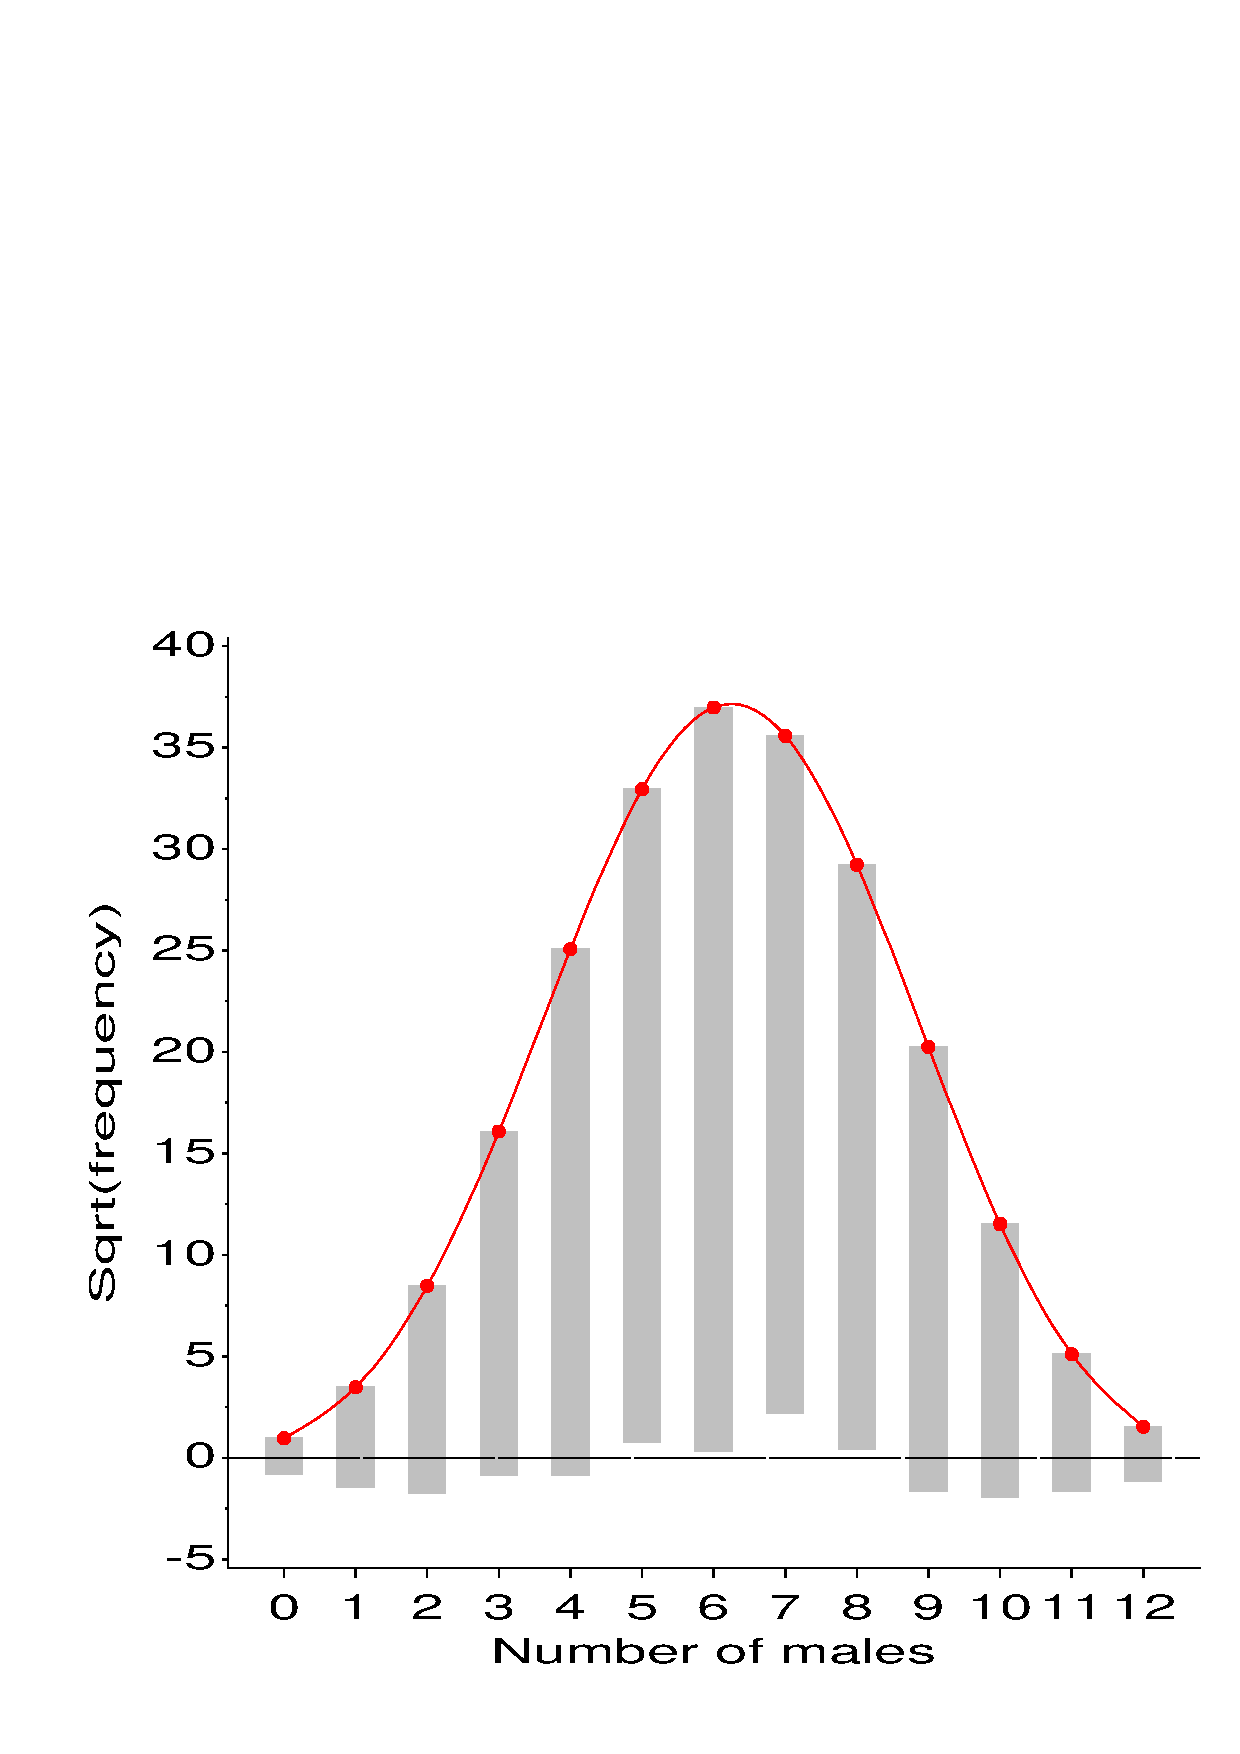
\includegraphics[width=1\linewidth]{saxony}\graphicsfile{ch2/fig/saxony.eps}{}
 \end{minipage}%
 \hfill
 \begin{minipage}[c]{.33\linewidth}
  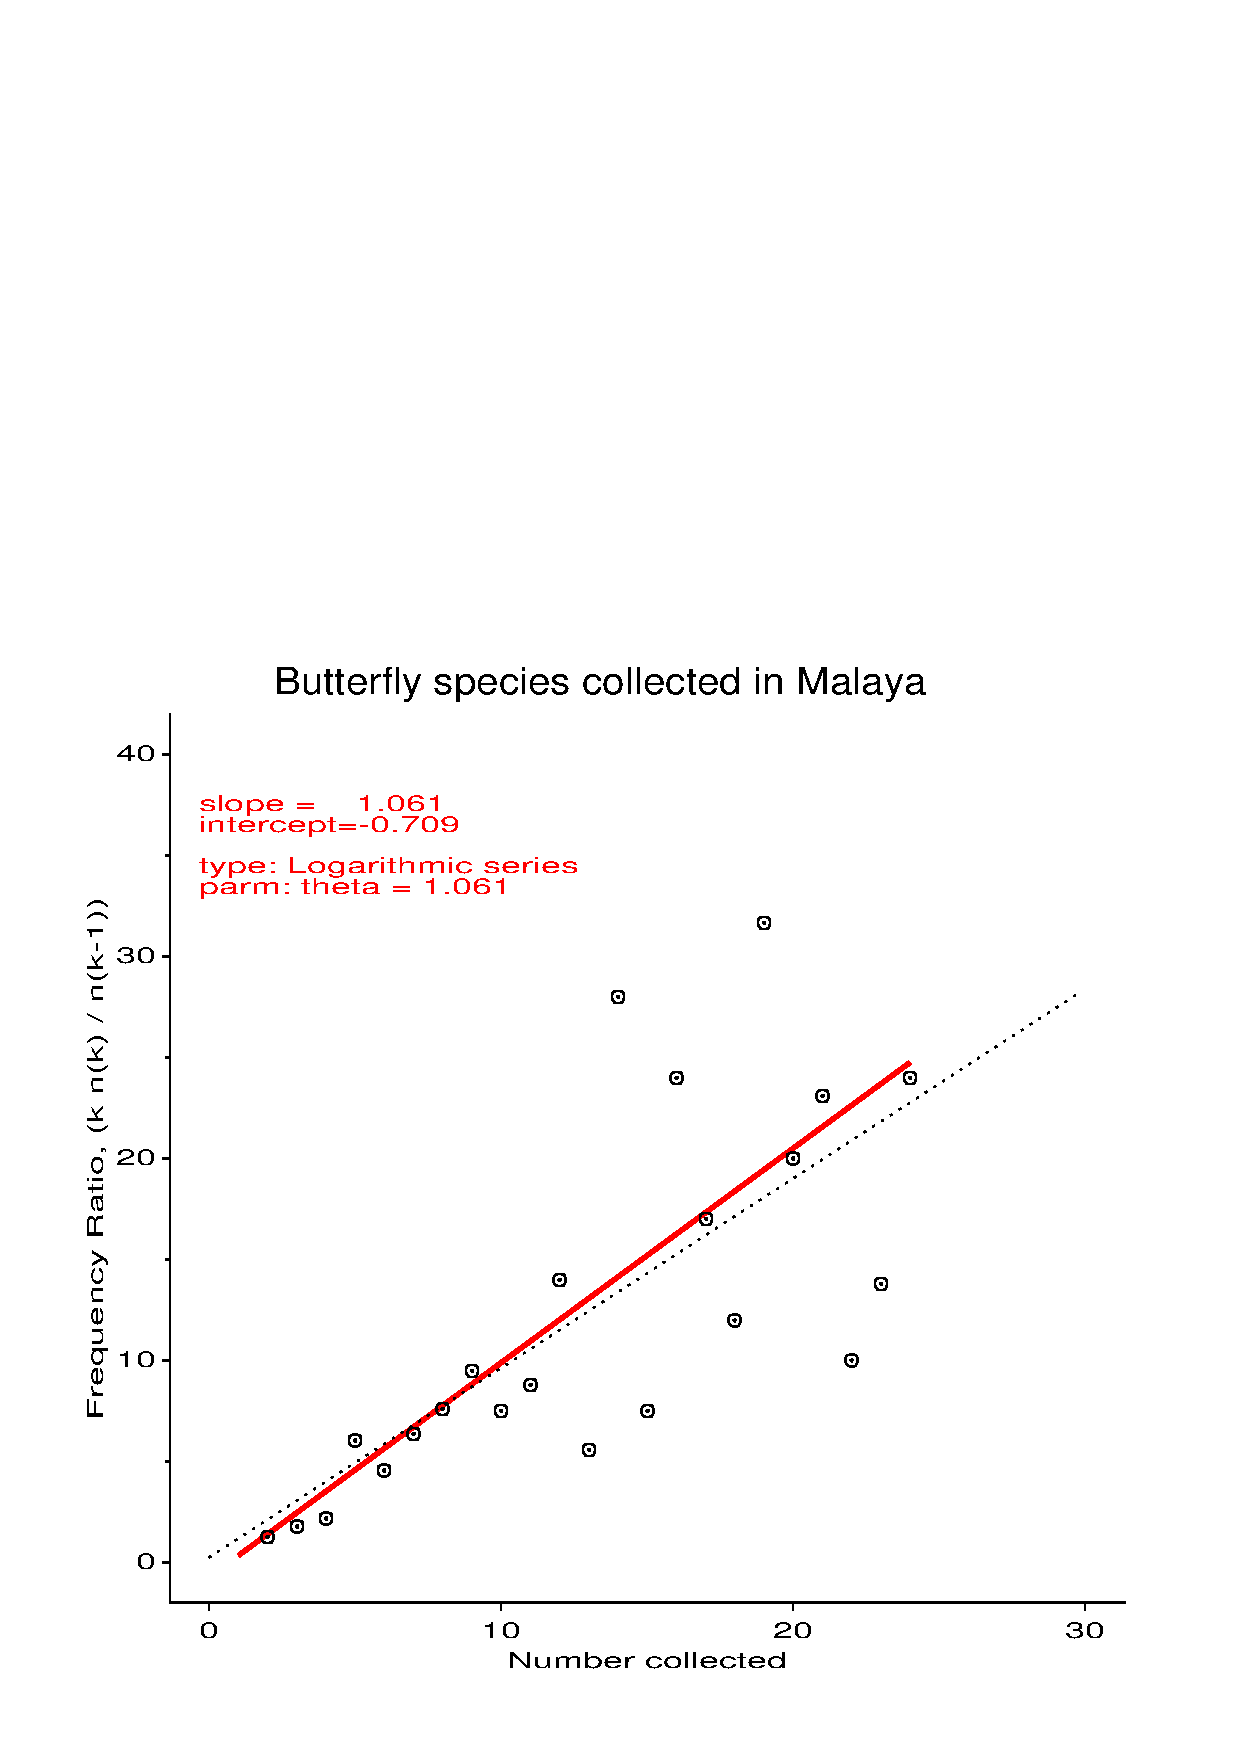
\includegraphics[width=1\linewidth]{orddemo3}\graphicsfile{ch2/fig/orddemo3.eps}{}
 \end{minipage}
 \hfill
 \begin{minipage}[c]{.33\linewidth}
  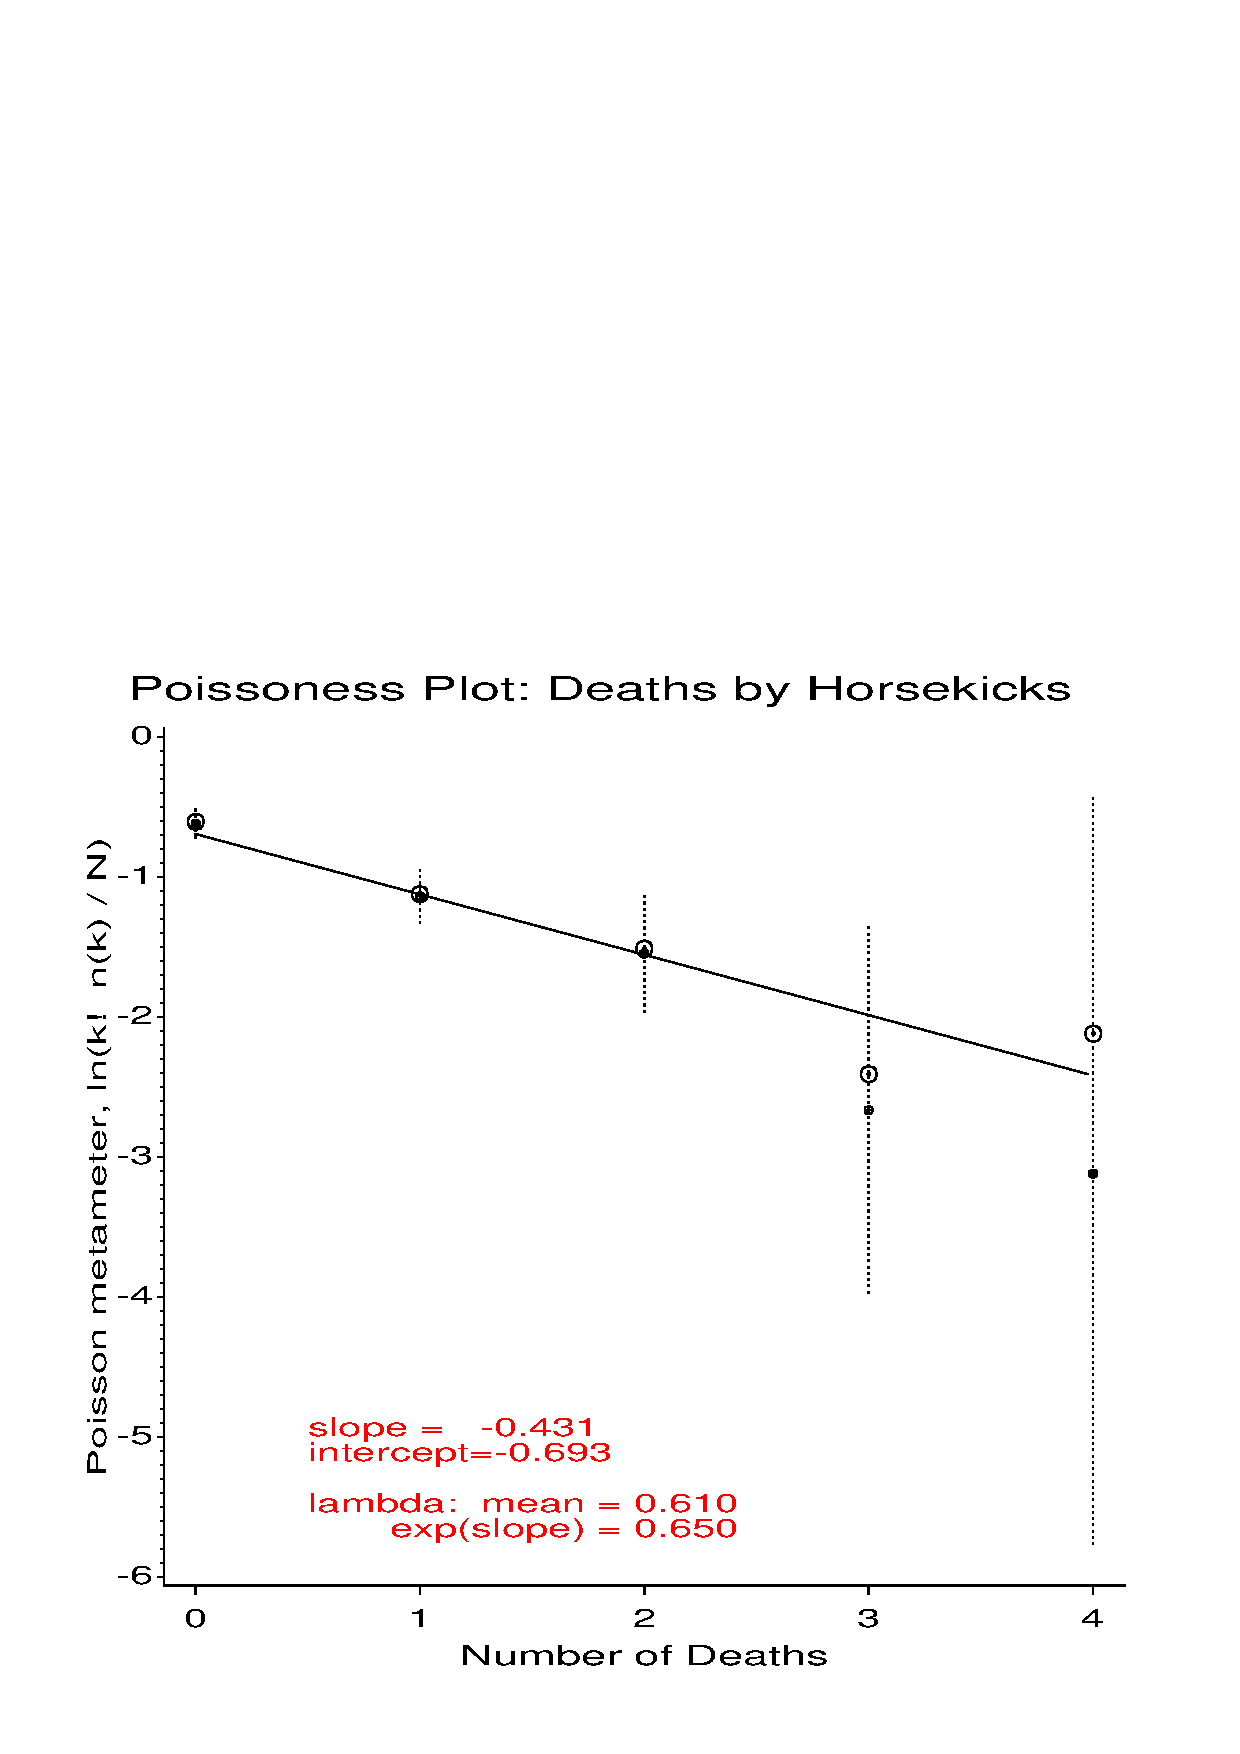
\includegraphics[width=1\linewidth]{poisdemo1}\graphicsfile{ch2/fig/poisdemo1.eps}{}
 \end{minipage}
\end{center}

   %% visual contents images

\chapterprelude{
Discrete data often follow various theoretical probability models.
Graphic displays are used to visualize goodness of fit,
to diagnose an appropriate model, and determine the impact of
individual observations on estimated parameters.
}
% \minitoc
% \clearpage

\epigraph{Not everything that counts can be counted, and not everything that
can be counted counts.}
{Albert Einstein}

Discrete frequency distributions often involve counts of occurrences of events,
such as accident fatalities, incidents of terrorism or suicide,
words in passages of text, or blood cells with some characteristic.
Often interest is focused on how closely such data follow a particular probability distribution,
such as the binomial, Poisson, or geometric distribution, which
provide the basis for generating mechanisms that might give rise to the
data.
Understanding and visualizing
such distributions
in the simplest case of an unstructured sample provides a building block for generalized
linear models (Chapter ?) where they serve as one component.  The also provide the basis for
a variety of recent extensions of regression models for count data (Chapter ?),
allowing excess counts of zeros (zero-inflated models), left- or right-
truncation often encountered in statistical practice.

This chapter describes the well-known discrete
frequency distributions: the binomial, Poisson, negative binomial,
geometric, and logarithmic series distributions in the simplest case of an unstructured sample.
The chapter begins with simple graphical displays (line graphs and bar charts) to view
the distributions of empirical data and theoretical frequencies from a specified
discrete distribution.

It then describes methods for fitting data to a distribution of a given form
and simple, effective
graphical methods than can be used used to visualize goodness of fit,
to diagnose an appropriate model (e.g., does a given data set follow the
Poisson or negative binomial?) and determine the impact of
individual observations on estimated parameters.

\section{Introduction to discrete distributions}\label{sec:discrete-intro}
Discrete data analysis is concerned with the study of the tabulation of one or
more types of events, often categorized into mutually exclusive and exhaustive
categories.  \term{Binary events} having two outcome categories include
the toss of a coin (head/tails), sex of a child (male/female), survival of
a patient following surgery (lived/died), and so forth.  \term{Polytomous events}
have more outcome categories, which may be \emph{ordered}
(rating of impairment: low/medium/high, by a physician)
and possibly numerically-valued 
(number of dots (pips), 1--6 on the toss of a die) 
or \emph{unordered} (political party supported: Liberal, Conservative, Greens, Socialist).

In this chapter, we focus largely on one-way frequency tables for a single 
numerically-valued variable.
Probability models for such data provide the opportunity to describe or explain
the \emph{structure} in such data, in that they entail some data generating 
mechanism and provide the basis for testing scientific hypotheses, prediction of
future results.  If a given probability model does not fit the data, this can often
be a further opportunity to extend understanding of the data or the underlying
substantive theory or both.

The remainder of this section gives a few substantive examples of situations where the 
well-known discrete frequency distributions (binomial, Poisson, negative binomial,
geometric, and logarithmic series) might reasonably apply, at least approximately.
The mathematical characteristics and properties of these theoretical
distributions are postponed to \secref{sec:discrete-distrib}.

In many cases, the data at hand pertain to two types of variables in a one-way
frequency table. There is a basic outcome variable, $k$, taking integer values,
$k = 0, 1, \dots$, and called a \term{count}.  For each value of $k$, we also have
a \term{frequency}, $n_k$ that the count $k$ was observed in some sample.
For example, in the study of children in families, the count variable
$k$ could be the total number of children or the number of male children;
the frequency variable, $n_k$, would then give the number of families with that
basic count $k$.

\subsection{Binomial data}\label{sec:binom-data}
Binomial type data arise as the discrete distribution of the number of
``success'' events in $n$ independent binary trials, each of which 
yields a success (yes/no, head/tail, lives/dies, male/female) with a constant probability $p$. 

Sometimes, as in \exref{ex:arbuthnot1}
below, the available data record only the number of successes
in $n$ trials, with separate such observations recorded over
time or space.  More commonly, as in \exref{ex:saxony1}
and \exref{ex:dice},
we have available data on the frequency $n_k$
of $k = 0, 1, 2, \dots n$ successes in the $n$ trials.


\begin{Example}[arbuthnot1]{Arbuthnot data}
Sex ratios--- births of male to female children have long been of interest
in population studies and demography. Indeed, in 1710, John Arbuthnot \citep{Arbuthnot:1710}
used data on the ratios of male to female christenings in London from 1629--1710 to carry out the first known significance test.
The data for these 82 years showed that in \emph{every} year there were more boys than girls.
He calculated that the under the assumption
that male and female births were equally likely, the probability of 82 years of
more males than females was vanishingly small,
 ($\Pr \approx 4.14 \times 10^{-25}$).  
He used this to argue that a nearly constant birth ratio $> 1$ (or $\Pr(\mathrm{Male}) > 0.5$)
could be interpreted to show the guiding hand of a divine being.

Arbuthnot's data, along with some other related variables 
are available in \data{Arbuthnot} in the \Rpackage{HistData}.
For now, we simply display a plot of the probability of a male birth over time.
The plot in \figref{fig:arbuthnot1} shows the proportion of males over years,
with horizontal lines at $\Pr(\mathrm{Male}) = 0.5$ and the mean,
$\Pr(\mathrm{Male}) = 0.517$.  Also shown is a (loess) smoothed curve, which suggests
that any deviation from a constant sex ratio is relatively small.
\begin{knitrout}
\definecolor{shadecolor}{rgb}{0.969, 0.969, 0.969}\color{fgcolor}\begin{kframe}
\begin{alltt}
\hlkwd{data}\hlstd{(Arbuthnot,} \hlkwc{package}\hlstd{=}\hlstr{"HistData"}\hlstd{)}
\hlkwd{with}\hlstd{(Arbuthnot, \{}
  \hlstd{prob} \hlkwb{=} \hlstd{Males}\hlopt{/}\hlstd{(Males}\hlopt{+}\hlstd{Females)}
  \hlkwd{plot}\hlstd{(Year, prob,} \hlkwc{type}\hlstd{=}\hlstr{'b'}\hlstd{,} \hlkwc{ylim}\hlstd{=}\hlkwd{c}\hlstd{(}\hlnum{0.5}\hlstd{,} \hlnum{0.54}\hlstd{),} \hlkwc{ylab}\hlstd{=}\hlstr{"Pr (Male)"}\hlstd{)}
  \hlkwd{abline}\hlstd{(}\hlkwc{h}\hlstd{=}\hlnum{0.5}\hlstd{,} \hlkwc{col}\hlstd{=}\hlstr{"red"}\hlstd{,} \hlkwc{lwd}\hlstd{=}\hlnum{2}\hlstd{)}
  \hlkwd{abline}\hlstd{(}\hlkwc{h}\hlstd{=}\hlkwd{mean}\hlstd{(prob),} \hlkwc{col}\hlstd{=}\hlstr{"blue"}\hlstd{)}
  \hlkwd{text}\hlstd{(}\hlkwc{x}\hlstd{=}\hlnum{1640}\hlstd{,} \hlkwc{y}\hlstd{=}\hlnum{0.5}\hlstd{,} \hlkwd{expression}\hlstd{(H[}\hlnum{0}\hlstd{]}\hlopt{:} \hlstr{"Pr(Male)=0.5"}\hlstd{),} \hlkwc{pos}\hlstd{=}\hlnum{3}\hlstd{,} \hlkwc{col}\hlstd{=}\hlstr{"red"}\hlstd{)}
  \hlstd{Arb.smooth} \hlkwb{<-} \hlkwd{loess.smooth}\hlstd{(Year,prob)}
  \hlkwd{lines}\hlstd{(Arb.smooth}\hlopt{$}\hlstd{x, Arb.smooth}\hlopt{$}\hlstd{y,} \hlkwc{col}\hlstd{=}\hlstr{"blue"}\hlstd{,} \hlkwc{lwd}\hlstd{=}\hlnum{2}\hlstd{)}
  \hlstd{\})}
\end{alltt}
\end{kframe}\begin{figure}[htbp]


\centerline{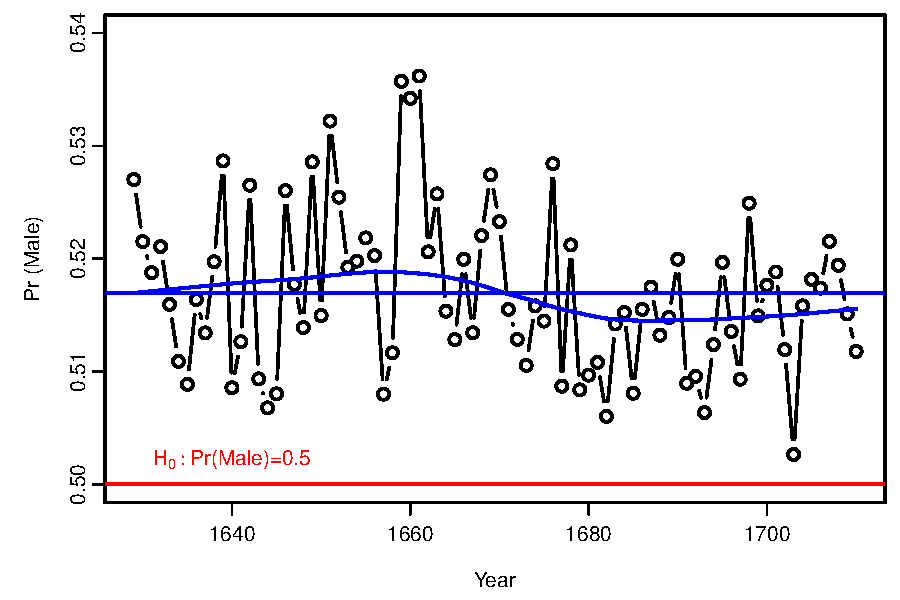
\includegraphics[width=.75\textwidth]{ch03/fig/arbuthnot1} }

\caption[Arbuthnot's data on male/female sex ratios]{Arbuthnot's data on male/female sex ratios in London, 1629--1710, together with a (loess) smoothed curve over time and the mean Pr(Male)\label{fig:arbuthnot1}}
\end{figure}


\end{knitrout}

We return to this data in a later chapter where we ask whether the variation around
the mean can be explained by any other considerations, or should just be considered 
random variation.
\end{Example}

\begin{Example}[saxony1]{Families in Saxony}
A related example of sex ratio data that ought to follow a binomial distribution
comes from a classic study by A. Geissler \citeyearpar{Geissler:1889}.
Geissler listed the data on the distributions of boys and girls in families
in Saxony for the period 1876--1885. In total, over four million births were
recorded, and the sex distribution in the family was available because the parents had to state the the sex of all their children on
the birth certificate.%

The complete data, classified by number of boys and number of girls
(each 0--12) appear in \citet[Table 1]{Edwards:1958}.%
\footnote{
\citet{Edwards:1958} notes that over these 10 years, many parents
will have had several children, and their family composition 
is therefore recorded more than once.  However, in families with a given
number of children, each family can appear only once.
}
\citet[Table 6.2]{Lindsey:95} selected only the 6115 families with 
12 children, and listed the frequencies by number of males.  The
data are shown in table form in \tabref{tab:saxtab} in the standard form
of a complete discrete distribution.  The basic outcome variable, 
$k = 0, 1, \dots, 12$, is the number of male children in a family
and the frequency variable, $n_k$ is the number of families with that
number of boys.

% latex table generated in R 3.0.1 by xtable 1.7-1 package
% Tue Nov 26 14:56:02 2013
\begin{table}[ht]
\caption{Number of male children in 6115 Saxony families of size 12} \label{tab:saxtab}
\centering
\begin{tabular}{l|rrrrrrrrrrrrrr}
  \hline
Males ($k$) & 0 & 1 & 2 & 3 & 4 & 5 & 6 & 7 & 8 & 9 & 10 & 11 & 12 & Sum \\ 
  \hline
Families ($n_k$) & 3 & 24 & 104 & 286 & 670 & 1,033 & 1,343 & 1,112 & 829 & 478 & 181 & 45 & 7 & 6,115 \\ 
   \hline
\end{tabular}
\end{table}
 


\figref{fig:saxony-barplot} shows a bar plot of the frequencies in \tabref{tab:saxtab}.
It can be seen that the distribution is quite symmetric.  The questions of interest
here are: 
(a) how close does the data follow a binomial distribution, with a constant
$\Pr(\mathrm{Male}) = p$?
(b) is there evidence to reject the hypothesis that $ p = 0.5$?

\begin{knitrout}
\definecolor{shadecolor}{rgb}{0.969, 0.969, 0.969}\color{fgcolor}\begin{kframe}
\begin{alltt}
\hlkwd{data}\hlstd{(Saxony,} \hlkwc{package}\hlstd{=}\hlstr{"vcd"}\hlstd{)}
\hlkwd{barplot}\hlstd{(Saxony,} \hlkwc{xlab}\hlstd{=}\hlstr{"Number of males"}\hlstd{,} \hlkwc{ylab}\hlstd{=}\hlstr{"Number of families"}\hlstd{,}
        \hlkwc{col}\hlstd{=}\hlstr{"lightblue"}\hlstd{,} \hlkwc{cex.lab}\hlstd{=}\hlnum{1.5}\hlstd{)}
\end{alltt}
\end{kframe}\begin{figure}[htbp]


\centerline{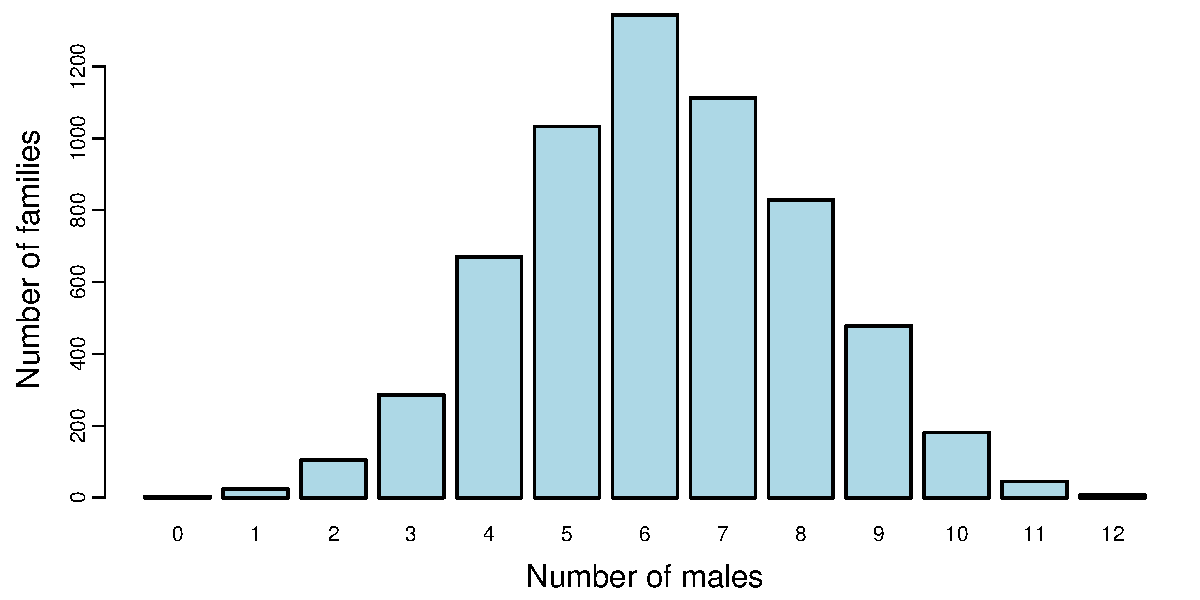
\includegraphics[width=.75\textwidth]{ch03/fig/saxony-barplot} }

\caption[Males in Saxony families of size 12]{Males in Saxony families of size 12\label{fig:saxony-barplot}}
\end{figure}


\end{knitrout}

\end{Example}

\begin{Example}[dice]{Weldon's dice}
Common examples of binomial distributions involve tossing coins
or dice, where some event outcome is considered a ``success''
and the number of successes ($k$) are are tabulated 
in a long series of trials to give the frequency ($n_k$) 
of each basic count, $k$.

Perhaps the most industrious dice-tosser of all times,
W. F. Raphael Weldon, an English evolutionary biologist
and joint founding editor of \emph{Biometrika} (with Francis Galton and Karl Pearson)
tallied the results of throwing 12 dice 26,306 times.
For his purposes, he considered the outcome of 5 or 6 pips showing on each die
to be a success to be a success, and all other outcomes as failures.

Weldon reported his results in a letter to Francis Galton dated
February 2, 1894, in order
``to judge whether the differences between a series of group frequencies
and a theoretical law \dots were more than might be attributed
to the chance fluctuations of random sampling''
\citep{KempKemp:91}.
In his seminal paper,
\citet{Pearson:00} used Weldon's data to illustrate the \chisq{} goodness-of-fit test, as did
\citet[Table 5.1, p. 121]{KendallStuart:63}.  

These data are
shown here as
\tabref{tab:dicetab},
in terms of the number of occurrences of a 5 or
6 in the throw of 12 dice.
If the dice were all identical and perfectly fair (balanced), one would
expect that $p = \Pr\{5 \textrm{ or } 6\} = \frac13$
and the distribution of the number of 5 or 6 would be binomial.

A peculiar feature of these data
as presented by Kendall and Stuart (not uncommon in discrete distributions)
is that the frequencies of 10--12 successes
are lumped together.%
\footnote{
The unlumped entries are, for (number of 5s or 6s: frequency) ---
(10: 14); (11: 4), (12:0),
given by \citet{Labby:2009}.
In this remarkable paper, Labby describes a mechanical device he constructed to 
repeat Weldon's experiment physically and automate the counting of outcomes.
He created electronics to roll 12 dice in a physical box, and hooked that
up to a webcam to capture an image of each toss and used image processing
software to record the counts.
}
This grouping must be taken into account in fitting
the distribution.  This dataset is available as \data{WeldonDice} in the
\Rpackage{vcd}.  The distribution is plotted in \figref{fig:dice}.

% latex table generated in R 3.0.1 by xtable 1.7-1 package
% Thu Nov 28 15:27:53 2013
\begin{table}[ht]
\centering
\caption{Frequencies of 5s or 6s in throws of 12 dice} \label{tab:dicetab}
\begin{tabular}{l|rrrrrrrrrrrr}
   \hline
\# 5s or 6s ($k$) & 0 & 1 & 2 & 3 & 4 & 5 & 6 & 7 & 8 & 9 & 10+ & Sum \\ 
Frequency ($n_k$) &   185 &  1,149 &  3,265 &  5,475 &  6,114 &  5,194 &  3,067 &  1,331 &   403 &   105 &    18 & 26,306 \\ 
   \hline
\end{tabular}
\end{table}



%%% one figure
%\begin{figure}[htb]
%%  \SASfig{dice.eps}{scale=.65}{dice}{Weldon's dice data}
%  \centering
%  \includegraphics[scale=.65]{dice.eps}
%  \caption{Weldon's dice data}%
%  \label{fig:dice}
%\end{figure}

\begin{knitrout}
\definecolor{shadecolor}{rgb}{0.969, 0.969, 0.969}\color{fgcolor}\begin{kframe}
\begin{alltt}
\hlkwd{data}\hlstd{(WeldonDice,} \hlkwc{package}\hlstd{=}\hlstr{"vcd"}\hlstd{)}
\hlkwd{dimnames}\hlstd{(WeldonDice)}\hlopt{$}\hlstd{n56[}\hlnum{11}\hlstd{]} \hlkwb{<-} \hlstr{"10+"}
\hlkwd{barplot}\hlstd{(WeldonDice,} \hlkwc{xlab}\hlstd{=}\hlstr{"Number of 5s and 6s"}\hlstd{,} \hlkwc{ylab}\hlstd{=}\hlstr{"Frequency"}\hlstd{,}
        \hlkwc{col}\hlstd{=}\hlstr{"lightblue"}\hlstd{,} \hlkwc{cex.lab}\hlstd{=}\hlnum{1.5}\hlstd{)}
\end{alltt}
\end{kframe}\begin{figure}[htbp]


\centerline{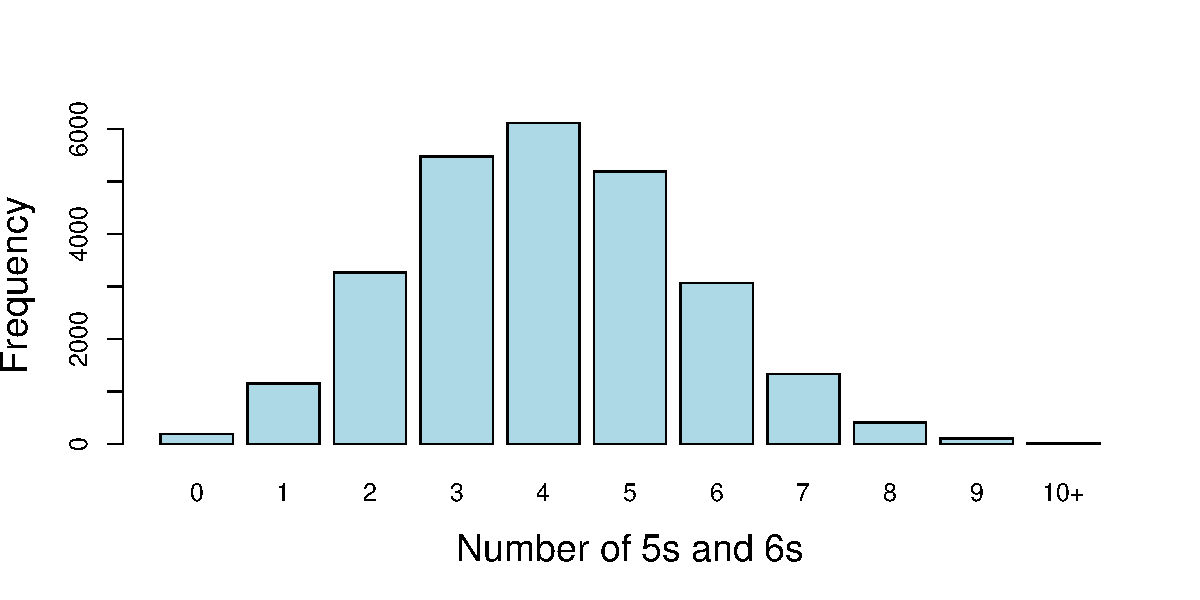
\includegraphics[width=.75\textwidth]{ch03/fig/dice} }

\caption[Weldon's dice data]{Weldon's dice data\label{fig:dice}}
\end{figure}


\end{knitrout}

\end{Example}

\subsection{Poisson data}\label{sec:pois-data}

Data of Poisson type arise when we observe the counts of events $k$ within a
fixed interval of time or space (length, area, volume) and tabulate their
frequencies, $n_k$.  For example, we may observe the number of radioactive
particles emitted by a source per second or number of births per hour,
or the number of tiger or whale sightings within some geographical regions.

In contrast to binomial data, where the counts are bounded below and above,
in Poisson data the counts $k$ are bounded below at 0, but can take integer
values with no fixed upper limit.
One defining characteristic for the Poisson distribution is for rare
events, which occur independently with a small and constant probability, $p$
in small intervals, and we count the number of such occurrences.

Several examples of data of this general type are given below.

\begin{Example}[horskick1]{Death by horse kick}
One of the oldest and best known examples of a Poisson distribution
is the data from
\citet{Bortkiewicz:98} on deaths of soldiers in the Prussian
army from kicks by horses and mules, shown in \tabref{tab:horsetab}.
Ladislaus von Bortkiewicz, an economist and statistician,
tabulated the number of soldiers in each of
14 army corps in the 20 years from 1875-1894
who died after being kicked by a horse
\citep[p. 18]{AndrewsHerzberg:85}.
\tabref{tab:horsetab} shows the data used by
\citet{Fisher:25} for 10 of these
army corps, summed over 20 years, giving 200
`corps-year' observations.  In 109 corps-years,
no deaths occurred; 65 corps-years had one death, etc.

The data set is available as \data{HorseKicks} in the \Rpackage{vcd}.
The distribution is plotted in \figref{fig:horsekicks}.
% latex table generated in R 3.0.1 by xtable 1.7-1 package
% Fri Nov 29 08:56:45 2013
\begin{table}[ht]
\centering
\caption{von Bortkiewicz's data on deaths by horse kicks} \label{tab:horsetab}
\begin{tabular}{l|rrrrr|r}
   \hline
Number of deaths ($k$) & 0 & 1 & 2 & 3 & 4 & Sum \\ 
  Frequency ($n_k$) & 109 &  65 &  22 &   3 &   1 & 200 \\ 
   \hline
\end{tabular}
\end{table}


\begin{knitrout}
\definecolor{shadecolor}{rgb}{0.969, 0.969, 0.969}\color{fgcolor}\begin{kframe}
\begin{alltt}
\hlkwd{data}\hlstd{(HorseKicks,} \hlkwc{package}\hlstd{=}\hlstr{"vcd"}\hlstd{)}
\hlkwd{barplot}\hlstd{(HorseKicks,} \hlkwc{xlab}\hlstd{=}\hlstr{"Number of deaths"}\hlstd{,} \hlkwc{ylab}\hlstd{=}\hlstr{"Frequency"}\hlstd{,}
        \hlkwc{col}\hlstd{=}\hlstr{"lightblue"}\hlstd{,} \hlkwc{cex.lab}\hlstd{=}\hlnum{1.5}\hlstd{)}
\end{alltt}
\end{kframe}\begin{figure}[htbp]


\centerline{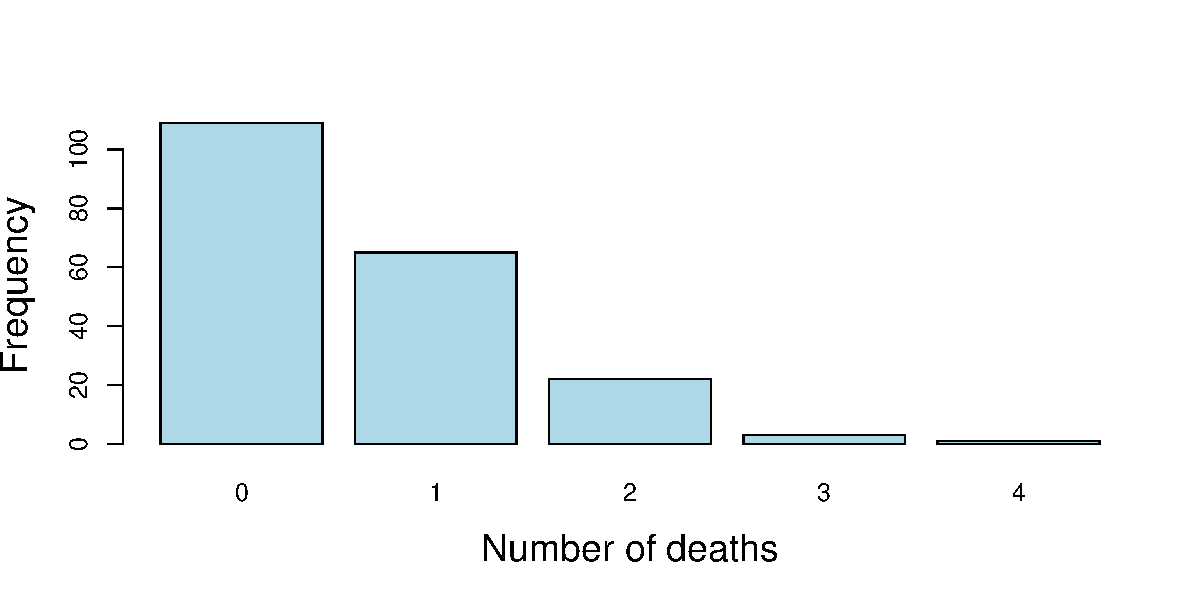
\includegraphics[width=.75\textwidth]{ch03/fig/horsekicks} }

\caption[HorseKicks data]{HorseKicks data\label{fig:horsekicks}}
\end{figure}


\end{knitrout}

\end{Example}

\begin{Example}[madison1]{Federalist papers}
In 1787--1788, Alexander Hamilton, John Jay, and James Madison
wrote a series of newspaper essays to persuade the voters of
New York State to ratify the U.S. Constitution.
The essays were titled \emph{The Federalist Papers}
and all were signed with the pseudonym ``Publius.''  Of the 77 papers published,
the author(s) of 65 are known, but \emph{both}
Hamilton and Madison later claimed sole authorship of the remaining 12.
\citet{MostellerWallace:63,MostellerWallace:84}
investigated the use of statistical methods to identify authors of
disputed works based on the frequency distributions of certain key
function words, and concluded that Madison had indeed authored the
12 disputed papers.%
\footnote{
It should be noted that this is a landmark work in the development and
application of statistical methods to the analysis of texts and
cases of disputed authorship. In addition to
\emph{may}, they considered many such marker words,
such as \emph{any}, \emph{by}, \emph{from}, \emph{upon}, and so forth.
Amonst these, the word \emph{upon} was the best discriminator between
the works known by Hamilton (3 per 1000 words) and Madison (1/6 per 1000 words).
In this work, they pioneered the use of Bayesian discriminant analysis,
and the use of cross-validation to assess the stability of estimates
and their conclusions.
}

\tabref{tab:fedtab} shows the distribution of the occurrence of one of
these ``marker'' words, 
the
word \emph{may} in 262 blocks of text (each about 200 words long)
from issues of the \emph{Federalist Papers} and other essays known
to be written by James Madison.  Read the table as follows:
in 156 blocks, the word \emph{may}
did not occur; it occurred once in 63 blocks, etc.  The distribution
is plotted in \figref{fig:federalist}.

% latex table generated in R 3.0.1 by xtable 1.7-1 package
% Fri Nov 29 14:25:47 2013
\begin{table}[htb]
\centering
\caption{Number of occurrences of the word \emph{may} in texts written by James Madison\label{tab:fedtab}} 
\begin{tabular}{l|rrrrrrr|r}
   \hline
Occurrences of \emph{may} ($k$) & 0 & 1 & 2 & 3 & 4 & 5 & 6 & Sum \\ 
  Blocks of text ($n_k$)       & 156 &  63 &  29 &   8 &   4 &   1 &   1 & 262 \\ 
   \hline
\end{tabular}
\end{table}

\begin{knitrout}
\definecolor{shadecolor}{rgb}{0.969, 0.969, 0.969}\color{fgcolor}\begin{kframe}
\begin{alltt}
\hlkwd{data}\hlstd{(Federalist,} \hlkwc{package}\hlstd{=}\hlstr{"vcd"}\hlstd{)}
\hlkwd{barplot}\hlstd{(Federalist,}
        \hlkwc{xlab}\hlstd{=}\hlstr{"Occurrences of 'may'"}\hlstd{,} \hlkwc{ylab}\hlstd{=}\hlstr{"Number of blocks of text"}\hlstd{,}
        \hlkwc{col}\hlstd{=}\hlstr{"lightgreen"}\hlstd{,} \hlkwc{cex.lab}\hlstd{=}\hlnum{1.5}\hlstd{)}
\end{alltt}
\end{kframe}\begin{figure}[htbp]


\centerline{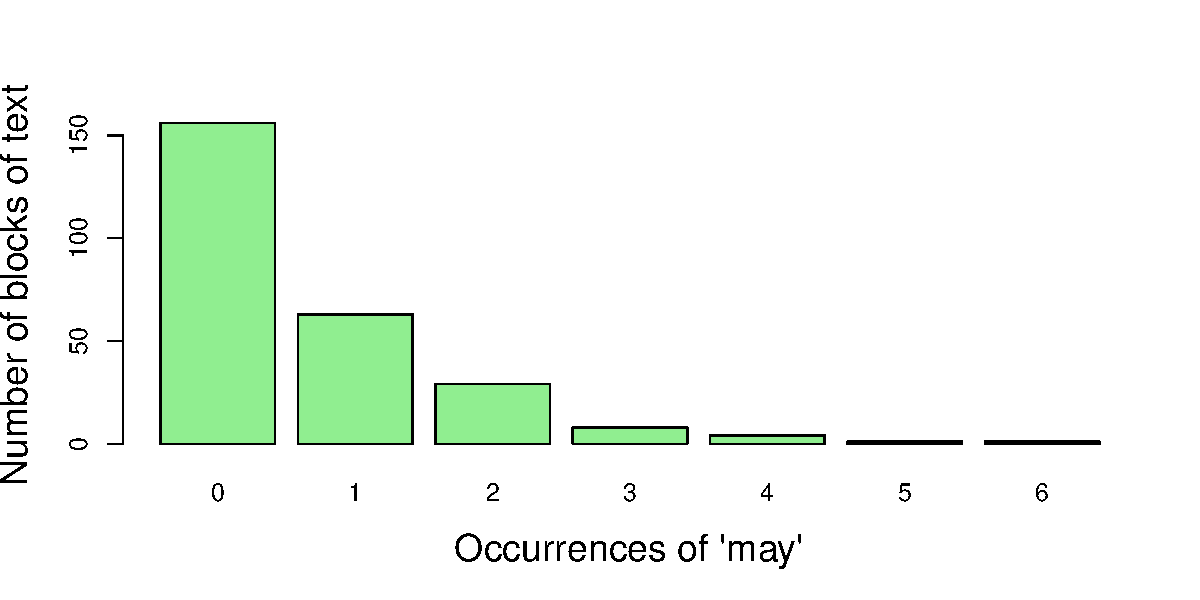
\includegraphics[width=.75\textwidth]{ch03/fig/federalist} }

\caption[Mosteller and Wallace Federalist data]{Mosteller and Wallace Federalist data\label{fig:federalist}}
\end{figure}


\end{knitrout}

\end{Example}

\begin{Example}[cyclists1]{London cycling deaths}

\citet{AberdeinSpiegelhalter:2013} observed that from November 5--13, 2013,
six people were killed while cycling in London.  How unusual is this
number of deaths in less than a two-week period?
Was this a freak occurrence, or should Londoners petition for
cycling lanes and greater road safety?
To answer these question, they obtained data from the 
UK Department of Transport \emph{Road Safety Data} from 2005--2012
and selected all accident fatalities of cyclists within the
cit of London.

It seems reasonable to assume that, in any short period of time, deaths of
people riding bicycles are independent events.  If, in addition, 
the probability of such events is constant over this time span,
the Poisson distribution should describe the distribution of
$0, 1, 2, 3, \dots$ deaths. Then, an answer to the main question can be
given in terms of the probability of six (or more) deaths in
a comparable period of time.

Their data, comprising 208 counts of deaths in the fortnightly periods
from January 2005 to December 2012 are contained in the \Dset
\data{CyclingDeaths} in \pkg{vcdExtra}.  To work with the
distribution, we first convert this to a one-way table.

\begin{knitrout}
\definecolor{shadecolor}{rgb}{0.969, 0.969, 0.969}\color{fgcolor}\begin{kframe}
\begin{alltt}
\hlkwd{data}\hlstd{(}\hlstr{"CyclingDeaths"}\hlstd{,} \hlkwc{package}\hlstd{=}\hlstr{"vcdExtra"}\hlstd{)}
\hlstd{CyclingDeaths.tab} \hlkwb{<-} \hlkwd{table}\hlstd{(CyclingDeaths}\hlopt{$}\hlstd{deaths)}
\hlstd{CyclingDeaths.tab}
\end{alltt}
\begin{verbatim}
## 
##   0   1   2   3 
## 114  75  14   5
\end{verbatim}
\end{kframe}
\end{knitrout}

The maximum number of deaths was 3, which occurred in only 5 two-week periods.
The distribution is plotted in \figref{fig:cyclists2}.
\begin{knitrout}
\definecolor{shadecolor}{rgb}{0.969, 0.969, 0.969}\color{fgcolor}\begin{kframe}
\begin{alltt}
\hlkwd{barplot}\hlstd{(CyclingDeaths.tab,}
        \hlkwc{xlab}\hlstd{=}\hlstr{"Number of deaths"}\hlstd{,} \hlkwc{ylab}\hlstd{=}\hlstr{"Number of fortnights"}\hlstd{,}
        \hlkwc{col}\hlstd{=}\hlstr{"pink"}\hlstd{,} \hlkwc{cex.lab}\hlstd{=}\hlnum{1.5}\hlstd{)}
\end{alltt}
\end{kframe}\begin{figure}[htbp]


\centerline{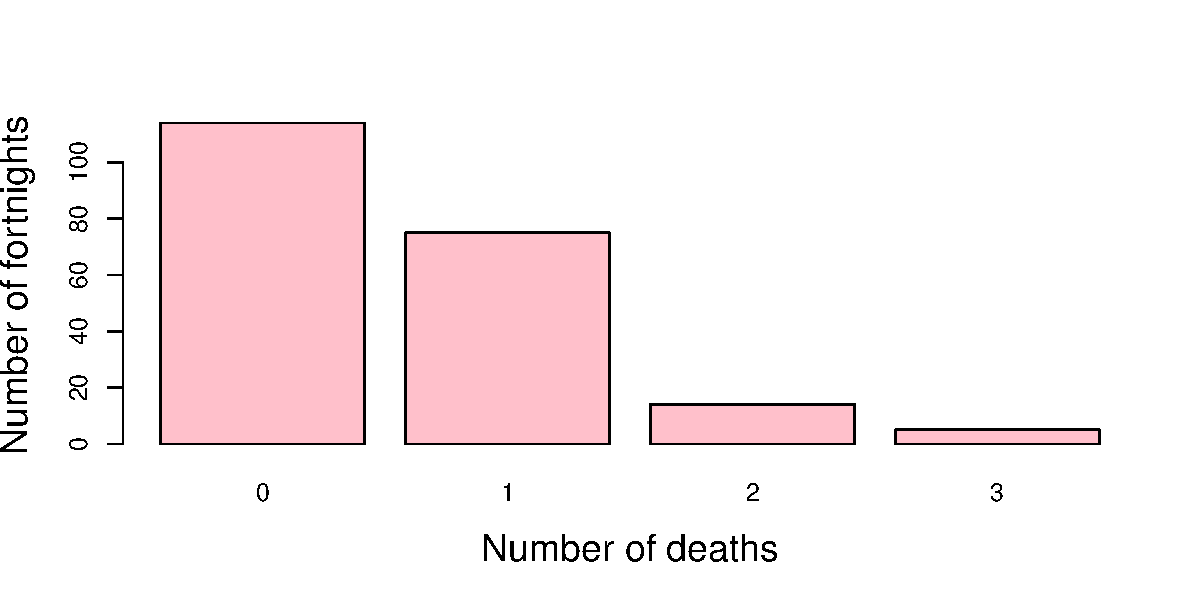
\includegraphics[width=.75\textwidth]{ch03/fig/cyclists2} }

\caption[Frequencies of number of cyclist deaths in two-week periods in London, 2005--2012]{Frequencies of number of cyclist deaths in two-week periods in London, 2005--2012\label{fig:cyclists2}}
\end{figure}


\end{knitrout}

We return to this data in \exref{ex:cyclists2} and answer the question of
how unusual six or more deaths would be in a Poisson distrution.

\end{Example}

\subsection{Type-token distributions}\label{sec:type-token}

There are a variety of other types of discrete data distributions.
One important class is \term{type-token} distributions, where
the basic count $k$ is the number of distinct types of some observed
event, $k = 1, 2, \dots$ and the frequency, $n_k$, is the number of
different instances observed.  For example, distinct words in a book,
words that subjects list as members of the semantic category ``fruit,''
musical notes that appear in a score, and species of animals caught
in traps can be considered as types, and the occurrences of
of those type comprise tokens.  

This class differs from the Poisson type considered above
in that the frequency for value $k=0$ is \emph{unobserved}.  Thus, questions like
(a) How many words did Shakespeare know?
(b) How many words in the English language are members of the
``fruit'' category?
(c) How many wolves remain in Canada's Northwest territories?
depend on the unobserved count for $k=0$. They 
cannot easily be answered without appeal to additional information
or statistical theory.


\begin{Example}[butterfly]{Butterfly species in Malaya}
In studies of the diversity of animal species, individuals are
collected and classified by species.
The distribution of the number of species (types) where $k = 1, 2, \dots$
individuals (tokens) were collected forms a kind of type-token distribution.
An early example of this kind of distribution was presented by
\citet{Fisher-etal:43}.
\tabref{tab:buttertab} lists the number of individuals of each of
501 species of butterfly collected in Malaya.
There were thus 118 species for which just a single instance was found,
74 species for which two individuals were found,
down to 3 species for which 24 individuals were collected.
Fisher et-al.\  note however that the distribution was truncated
at $k = 24$.
Type-token distributions are often J-shaped, with a long upper tail,
as we see in \figref{fig:butterfly}.
% latex table generated in R 3.0.1 by xtable 1.7-1 package
% Wed Nov 27 17:25:33 2013
%\begin{table}[ht]
%\centering
%\caption{Number of butterfly species $n_k$ for which $k$ individuals were collected} 
%\begin{tabular}{l|rrrrrrrrrrrrr rrrrrrrrrrrr}
%   \hline
%Individuals ($k$) & 1 & 2 & 3 & 4 & 5 & 6 & 7 & 8 & 9 & 10 & 11 & 12 
%                  & 13 & 14 & 15 & 16 & 17 & 18 & 19 & 20 & 21 & 22 & 23 & 24 & Sum \\ 
%   \hline
%Species ($n_k$) & 118 &  74 &  44 &  24 &  29 &  22 &  20 &  19 &  20 &  15 &  12 &  14 
%                &   6 &  12 &   6 &   9 &   9 &   6 &  10 &  10 &  11 &   5 &   3 &   3 & 501 \\ 
%  \end{tabular}
%\end{table}

%% hand edited to use two rows per line 
\begin{table}[ht]
\centering
\caption{Number of butterfly species $n_k$ for which $k$ individuals were collected} \label{tab:buttertab}
\begin{tabular}{l|rrrrrrrrrrrr|r}
   \hline
Individuals ($k$) & 1 & 2 & 3 & 4 & 5 & 6 & 7 & 8 & 9 & 10 & 11 & 12 \\
Species ($n_k$)   & 118 &  74 &  44 &  24 &  29 &  22 &  20 &  19 &  20 &  15 &  12 &  14 \\
   \hline \hline
Individuals ($k$) & 13 & 14 & 15 & 16 & 17 & 18 & 19 & 20 & 21 & 22 & 23 & 24 & Sum \\ 
Species ($n_k$)   &   6 &  12 &   6 &   9 &   9 &   6 &  10 &  10 &  11 &   5 &   3 &   3 & 501 \\ 
   \hline
  \end{tabular}
\end{table}

 


\begin{knitrout}
\definecolor{shadecolor}{rgb}{0.969, 0.969, 0.969}\color{fgcolor}\begin{kframe}
\begin{alltt}
\hlkwd{data}\hlstd{(Butterfly,} \hlkwc{package}\hlstd{=}\hlstr{"vcd"}\hlstd{)}
\hlkwd{barplot}\hlstd{(Butterfly,} \hlkwc{xlab}\hlstd{=}\hlstr{"Number of individuals"}\hlstd{,} \hlkwc{ylab}\hlstd{=}\hlstr{"Number of species"}\hlstd{,}
        \hlkwc{cex.lab}\hlstd{=}\hlnum{1.5}\hlstd{)}
\end{alltt}
\end{kframe}\begin{figure}[htbp]


\centerline{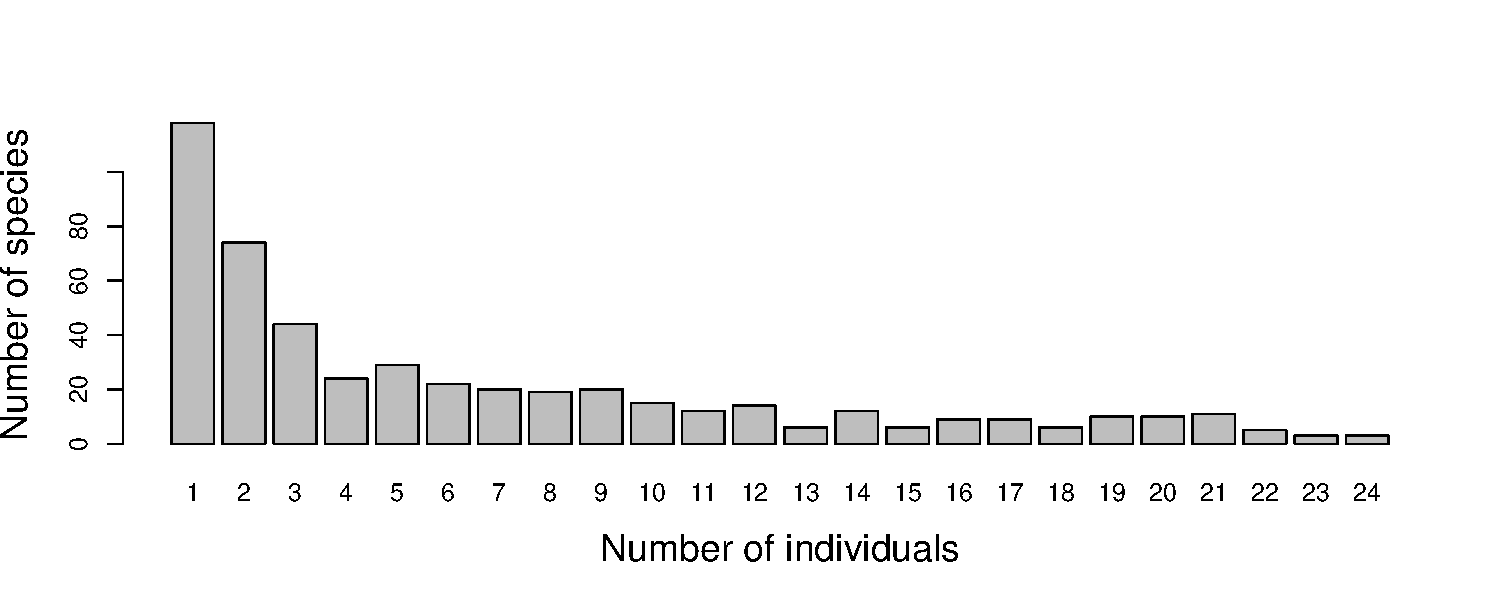
\includegraphics[width=.9\textwidth]{ch03/fig/butterfly} }

\caption[Butterfly species in Malaya]{Butterfly species in Malaya\label{fig:butterfly}}
\end{figure}


\end{knitrout}


\end{Example}


\section{Characteristics of  discrete distributions}\label{sec:discrete-distrib}
This section briefly reviews the characteristics of some of the
important discrete distributions encountered in practice and illustrates their
use with \R.
An overview of these distributions is shown in \tabref{tab:distns}.
For more detailed information on these and other discrete distributions,
\citet{Johnson-etal:92} and \citet{WimmerAltman:1999:thesaurus}
present the most comprehensive treatments;
\citet[\C 2]{Zelterman:99} gives a compact summary.

\begin{table}[htbp]%
\caption{Discrete probability distributions\label{tab:distns}}%
\small
\centering
\begin{tabular}{lll}\hline
Discrete     & Probability  & parameter(s)  \\ 
Distribution & function, $p(k)$  
\\ \hline
%
Binomial & $\binom nk p^k(1-p)^{n-k}$ & \brk{$p$=Pr (success);\\ $n$=\# trials} \\[1ex] 
Poisson & $e^{-\lambda }\lambda ^k/k!$ & $\lambda$= mean  \\[1ex] 
Negative binomial & $\binom{n+k-1}kp^n(1-p)^k$ &  $p$, $n$  \\[1ex] 
Geometric & $p(1-p)^k$ &  $p$  \\[1ex]
Logarithmic series & $\theta ^k/[-k\log (1-\theta )]$ &  $\theta$ \\[1ex] \hline
\end{tabular}
\end{table}%



For each distribution, we describe properties and generating
mechanisms, and show how its parameters can be estimated
and how to plot the frequency distribution.  \R has a wealth of
functions for a wide variety of distributions.  For ease of reference,
their names and types for the distributions covered here are shown
in \tabref{tab:distfuns}. The naming scheme is simple and easy to
remember:  for each distribution, there are functions, with a prefix
letter, \code{d}, \code{p}, \code{q}, \code{r}, followed by the
name for that class of distribution:%
\footnote{The CRAN Task View on Probability Distributions,
\url{http://cran.r-project.org/web/views/Distributions.html},
provides a general overview and lists a wide variety of contributed
packages for specialized distributions, discrete and continuous.}
\begin{description*}
  \item[d] a density function,%
\footnote{
For discrete random variables this is usually called the probability mass function (pmf).
}
  $\Pr \{X = x\} \equiv p(x)$
for the probability that the variable $X$ takes the value $x$.
  \item[p] a cumulative probability function, or CDF, 
  $F(x) = \sum_{X\le x} p(x)$.
  \item[q] a quantile function, the inverse of the CDF, $x = F^{-1} (p)$. 
  The quantile  is defined as the smallest value $x$ such that $F(x) \ge p$. 
  \item[r] a random number generating function for that distribution.
\end{description*}
In the \R console, \code{help(Distributions)} gives an overview listing of
the distribution functions available in the \Rpackage{stats}.

\begin{table}[htbp]%
\caption{\R functions for discrete probability distributions\label{tab:distfuns}}%
%\small
\centering
\begin{tabular}{l|llll}\hline
Discrete     & Density (pmf)    & Cumulative  & Quantile & Random \# \\ 
distribution & function         & (CDF)  & CDF$^{-1}$ & generator \\  
\hline
%
Binomial          & \func{dbinom} & \func{pbinom} & \func{qbinom}  & \func{rbinom}  \\[0.5ex] 
Poisson           & \func{dpois} & \func{ppois} & \func{qpois}  & \func{rpois}  \\[0.5ex] 
Negative binomial & \func{dnbinom} & \func{pnbinom} & \func{qnbinom}  & \func{rnbinom}  \\[0.5ex] 
Geometric         & \func{dgeom} & \func{pgeom} & \func{qgeom}  & \func{rgeom}  \\[0.5ex]
Logarithmic series& \func{dlogseries} & \func{plogseries} & \func{qlogseries}  & \func{rlogseries}  \\[0.5ex]
\hline
\end{tabular}
\end{table}%




\subsection{The binomial distribution}\label{sec:binomial}
\ix{binomial distribution|(}
The binomial distribution, $\Bin(n, p)$, 
arises as the distribution of the
number of events of interest which occur in $n$ independent trials
when the probability of the event on any one trial is the constant
value $p = \Pr ( \textrm{event} )$.
For example, if 15\% of the population has red hair,
the number of red-heads in randomly sampled groups of $n=10$
might follow a binomial distribution, $\Bin(10, 0.15)$;
in Weldon's dice data (\exref{ex:dice}), the probability of
a 5 or 6 should be $\frac13$ on any one trial, and
the number of 5s or 6s in tosses of 12 dice would follow
$\Bin(12, \frac13)$.

Over $n$ independent trials, the number of events  $k$
may range from 0 to $n$; if $X$ is a random variable
with a binomial distribution, the probability that $X = k$ is given
by
\begin{equation}\label{eq:binom}
\Bin(n,p): \Pr \{ X = k \} \equiv p ( k )  =
{n \choose k} p^k (1-p)^{n-k}
  \quad\quad k = 0, 1, \dots, n
  \comma
\end{equation}
where ${n \choose k} = n! / k! (n - k)!$ is the number of ways
of choosing $k$ out of $n$.
The first three (central) moments of the binomial distribution are
as follows 
(letting $q = 1 - p$),
\begin{eqnarray*}
\textrm{Mean}[X] & = & n p  \\
\textrm{Var}[X] &  = & n p q \\
\textrm{Skew}[X] & = & n p q (q - p) 
\period
\end{eqnarray*}
It is easy to verify that
the binomial distribution has its maximum variance when $p = \frac12$.
It is symmetric (Skew[X]=0) when $p = \frac12$, and negatively (positively)
skewed when $p < \frac12$ ($p > \frac12$ ).

If we are given data in the form of a discrete (binomial) distribution
(and $n$ is known),
then the maximum likelihood estimator of $p$ can be obtained
as the weighted mean of the values $k$ with weights $n_k$,
\begin{equation*}% \label{eq:binp}
\hat{p} = \frac{\bar{x}}{n} =
  \frac{(\sum_{k} k \times n_k ) / \sum_k n_k}{n}
  \comma
\end{equation*}
and has sampling variance $Var(\hat{p}) = pq/n$.

\subsubsection{Calculation and visualization}
As indicated in \tabref{tab:distfuns} (but without listing the
parameters of these functions), 
binomial probabilities
can be calculated with \code{dbinom(x, n, p)}, 
where \code{x} is a vector of the number of successes in \code{n}
trials and \code{p} is the probability of success on any one trial.
Cumulative probabilities, summed up to a vector of quantiles, \code{Q}
can be calculated with \code{pbinom(Q, n, p)},
and the quantiles (the smallest value $x$ such that $F(x) \ge P$)
with \code{qbinom(P, n, p)}.
To generate \code{N} random observations from a binomial distribution
with \code{n} trials and success probability \code{p}
use \code{rbinom(N, n, p)}.


For example, to find and plot the binomial probabilities corresponding
to Weldon's tosses of 12 dice, with $n=0, \dots 12$ and $p=\frac13$,
we could do the following
\begin{knitrout}
\definecolor{shadecolor}{rgb}{0.969, 0.969, 0.969}\color{fgcolor}\begin{kframe}
\begin{alltt}
\hlstd{x} \hlkwb{<-} \hlkwd{seq}\hlstd{(}\hlnum{0}\hlstd{,} \hlnum{12}\hlstd{)}
\hlkwd{plot}\hlstd{(}\hlkwc{x}\hlstd{=x,} \hlkwc{y}\hlstd{=}\hlkwd{dbinom}\hlstd{(x,}\hlnum{12}\hlstd{,}\hlnum{1}\hlopt{/}\hlnum{3}\hlstd{),} \hlkwc{type}\hlstd{=}\hlstr{"h"}\hlstd{,}
  \hlkwc{xlab}\hlstd{=}\hlstr{"Number of successes"}\hlstd{,} \hlkwc{ylab}\hlstd{=}\hlstr{"Probability"}\hlstd{,}
        \hlkwc{lwd}\hlstd{=}\hlnum{8}\hlstd{,} \hlkwc{lend}\hlstd{=}\hlstr{"square"}\hlstd{)}
\hlkwd{lines}\hlstd{(}\hlkwc{x}\hlstd{=x,} \hlkwc{y}\hlstd{=}\hlkwd{dbinom}\hlstd{(x,}\hlnum{12}\hlstd{,}\hlnum{1}\hlopt{/}\hlnum{3}\hlstd{))}
\end{alltt}
\end{kframe}\begin{figure}[htbp]


\centerline{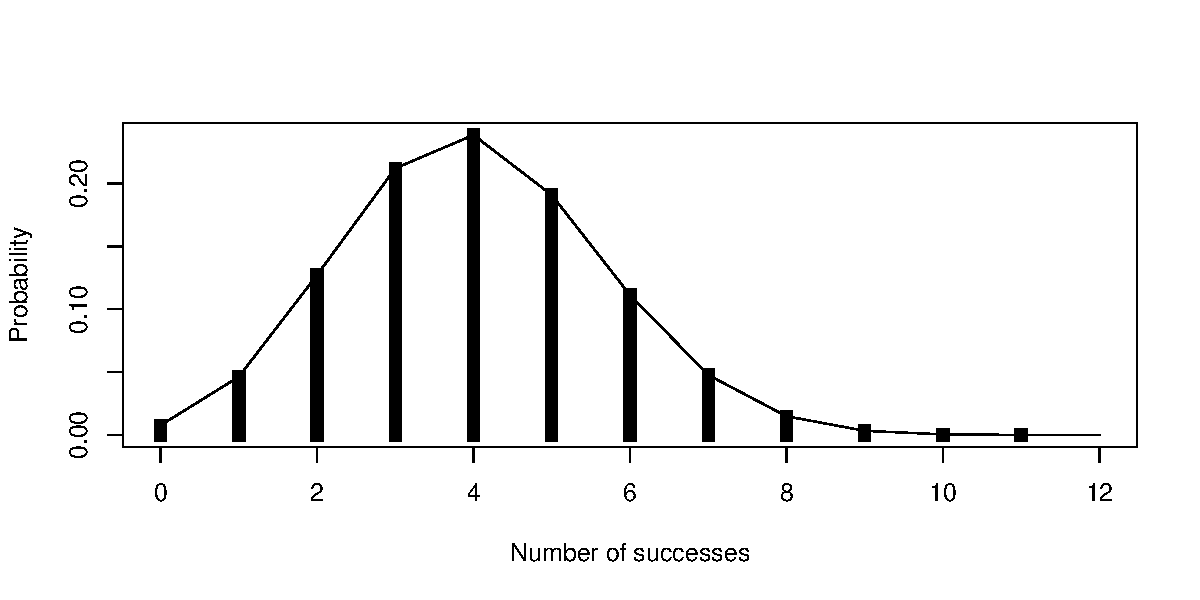
\includegraphics[width=.75\textwidth]{ch03/fig/dbinom1} }

\caption[Binomial distribution for n=0--12 trials and p=1/3]{Binomial distribution for n=0--12 trials and p=1/3\label{fig:dbinom1}}
\end{figure}


\end{knitrout}

Note that in the call to \func{plot}, \code{type="h"} draws histogram type
lines to the bottom of the vertical axis, and \code{lwd=8} makes them wide.
The call to \func{lines} shows another way to plot the data, as a probability
polygon. We illustrate other styles for plotting in \secref{sec:poisson},
\exref{ex:dpois-plot} below.

\begin{Example}[dice2]{Weldon's dice}
Going a bit further, we can compare Weldon's data with the 
theoretical binomial distribution as shown below. Because the
\data{WeldonDice} data collapsed the frequencies for 10--12
successes as $10+$,
we do the same with the binomial probabilities.
The expected frequencies (\code{Exp}), if Weldon's dice tosses obeyed
the binomial distribution are calculated as $N \times p(k)$ for
$N=26306$ tosses.  The $\chisq$ test for goodness of fit
is described later in \secref{sec:discrete-fit}, but a glance
at the \code{Diff} column shows that these are all negative for
$k=0, \dots 4$ and positive thereafter.

\begin{knitrout}
\definecolor{shadecolor}{rgb}{0.969, 0.969, 0.969}\color{fgcolor}\begin{kframe}
\begin{alltt}
\hlstd{Weldon.df} \hlkwb{<-} \hlkwd{as.data.frame}\hlstd{(WeldonDice)}   \hlcom{# convert to data frame}

\hlstd{x} \hlkwb{<-} \hlkwd{seq}\hlstd{(}\hlnum{0}\hlstd{,} \hlnum{12}\hlstd{)}
\hlstd{Prob} \hlkwb{<-} \hlkwd{dbinom}\hlstd{(x,} \hlnum{12}\hlstd{,} \hlnum{1}\hlopt{/}\hlnum{3}\hlstd{)}               \hlcom{# binomial probabilities}
\hlstd{Prob} \hlkwb{<-} \hlkwd{c}\hlstd{(Prob[}\hlnum{1}\hlopt{:}\hlnum{10}\hlstd{],} \hlkwd{sum}\hlstd{(Prob[}\hlnum{11}\hlopt{:}\hlnum{13}\hlstd{]))}  \hlcom{# sum values for 10+}
\hlstd{Exp}\hlkwb{=} \hlkwd{round}\hlstd{(}\hlnum{26306}\hlopt{*}\hlstd{Prob)}                   \hlcom{# expected frequencies}
\hlstd{Diff} \hlkwb{=} \hlstd{Weldon.df[,}\hlstr{"Freq"}\hlstd{]} \hlopt{-} \hlstd{Exp}          \hlcom{# raw residuals}
\hlstd{Chisq} \hlkwb{=} \hlstd{Diff}\hlopt{^}\hlnum{2} \hlopt{/}\hlstd{Exp}
\hlkwd{data.frame}\hlstd{(Weldon.df,} \hlkwc{Prob}\hlstd{=}\hlkwd{round}\hlstd{(Prob,}\hlnum{5}\hlstd{), Exp, Diff, Chisq)}
\end{alltt}
\begin{verbatim}
##    n56 Freq    Prob  Exp Diff  Chisq
## 1    0  185 0.00771  203  -18 1.5961
## 2    1 1149 0.04624 1216  -67 3.6916
## 3    2 3265 0.12717 3345  -80 1.9133
## 4    3 5475 0.21195 5576 -101 1.8294
## 5    4 6114 0.23845 6273 -159 4.0301
## 6    5 5194 0.19076 5018  176 6.1730
## 7    6 3067 0.11127 2927  140 6.6963
## 8    7 1331 0.04769 1255   76 4.6024
## 9    8  403 0.01490  392   11 0.3087
## 10   9  105 0.00331   87   18 3.7241
## 11 10+   18 0.00054   14    4 1.1429
\end{verbatim}
\end{kframe}
\end{knitrout}

\end{Example}

Finally, we can use programming features in \R to calculate and plot
probabilities for binomial distributions over a range of
both \code{x} and \code{p} as follows, for the purposes of
graphing the distributions as one or both varies.
The following code uses \func{expand.grid} to create a data frame \code{XP}
containing all combinations of \code{x=0:12} and 
\code{p=c(1/6, 1/3, 1/2, 2/3)}. These values are then supplied as
arguments to \func{dbinom}.  For the purpose of plotting,
the decimal value of \code{p} is declared as a factor.

\begin{knitrout}
\definecolor{shadecolor}{rgb}{0.969, 0.969, 0.969}\color{fgcolor}\begin{kframe}
\begin{alltt}
\hlstd{XP} \hlkwb{<-}\hlkwd{expand.grid}\hlstd{(}\hlkwc{x}\hlstd{=}\hlnum{0}\hlopt{:}\hlnum{12}\hlstd{,} \hlkwc{p}\hlstd{=}\hlkwd{c}\hlstd{(}\hlnum{1}\hlopt{/}\hlnum{6}\hlstd{,} \hlnum{1}\hlopt{/}\hlnum{3}\hlstd{,} \hlnum{1}\hlopt{/}\hlnum{2}\hlstd{,} \hlnum{2}\hlopt{/}\hlnum{3}\hlstd{))}
\hlstd{bin.df} \hlkwb{<-} \hlkwd{data.frame}\hlstd{(XP,} \hlkwc{prob}\hlstd{=}\hlkwd{dbinom}\hlstd{(XP[,}\hlstr{"x"}\hlstd{],} \hlnum{12}\hlstd{, XP[,}\hlstr{"p"}\hlstd{]))}
\hlstd{bin.df}\hlopt{$}\hlstd{p} \hlkwb{<-} \hlkwd{factor}\hlstd{(bin.df}\hlopt{$}\hlstd{p,} \hlkwc{labels}\hlstd{=}\hlkwd{c}\hlstd{(}\hlstr{"1/6"}\hlstd{,} \hlstr{"1/3"}\hlstd{,} \hlstr{"1/2"}\hlstd{,} \hlstr{"2/3"}\hlstd{))}
\hlkwd{str}\hlstd{(bin.df)}
\end{alltt}
\begin{verbatim}
## 'data.frame':	52 obs. of  3 variables:
##  $ x   : int  0 1 2 3 4 5 6 7 8 9 ...
##  $ p   : Factor w/ 4 levels "1/6","1/3","1/2",..: 1 1 1 1 1 1 1 1 1 1 ...
##  $ prob: num  0.1122 0.2692 0.2961 0.1974 0.0888 ...
\end{verbatim}
\end{kframe}
\end{knitrout}


This data can be plotted using \func{xyplot} in \pkg{lattice},
using the \code{groups} argument to make separate curves for each
value of \code{p}.  The following code generates \figref{fig:dbinom2-plot}.
\begin{knitrout}
\definecolor{shadecolor}{rgb}{0.969, 0.969, 0.969}\color{fgcolor}\begin{kframe}
\begin{alltt}
\hlkwd{library}\hlstd{(lattice)}
\hlstd{mycol} \hlkwb{<-} \hlkwd{palette}\hlstd{()[}\hlnum{2}\hlopt{:}\hlnum{5}\hlstd{]}
\hlkwd{xyplot}\hlstd{( prob} \hlopt{~} \hlstd{x,} \hlkwc{data}\hlstd{=bin.df,} \hlkwc{groups}\hlstd{=p,}
  \hlkwc{xlab}\hlstd{=}\hlkwd{list}\hlstd{(}\hlstr{'Number of successes'}\hlstd{,} \hlkwc{cex}\hlstd{=}\hlnum{1.25}\hlstd{),}
  \hlkwc{ylab}\hlstd{=}\hlkwd{list}\hlstd{(}\hlstr{'Probability'}\hlstd{,}  \hlkwc{cex}\hlstd{=}\hlnum{1.25}\hlstd{),}
  \hlkwc{type}\hlstd{=}\hlstr{'b'}\hlstd{,} \hlkwc{pch}\hlstd{=}\hlnum{15}\hlopt{:}\hlnum{17}\hlstd{,} \hlkwc{lwd}\hlstd{=}\hlnum{2}\hlstd{,} \hlkwc{cex}\hlstd{=}\hlnum{1.25}\hlstd{,} \hlkwc{col}\hlstd{=mycol,}
  \hlkwc{key} \hlstd{=} \hlkwd{list}\hlstd{(}
    \hlkwc{title} \hlstd{=} \hlstr{'Pr(success)'}\hlstd{,}
    \hlkwc{points} \hlstd{=} \hlkwd{list}\hlstd{(}\hlkwc{pch}\hlstd{=}\hlnum{15}\hlopt{:}\hlnum{17}\hlstd{,} \hlkwc{col}\hlstd{=mycol,} \hlkwc{cex}\hlstd{=}\hlnum{1.25}\hlstd{),}
    \hlkwc{lines} \hlstd{=} \hlkwd{list}\hlstd{(}\hlkwc{lwd}\hlstd{=}\hlnum{2}\hlstd{,} \hlkwc{col}\hlstd{=mycol),}
    \hlkwc{text} \hlstd{=} \hlkwd{list}\hlstd{(}\hlkwd{levels}\hlstd{(bin.df}\hlopt{$}\hlstd{p)),}
    \hlkwc{x}\hlstd{=}\hlnum{0.9}\hlstd{,} \hlkwc{y}\hlstd{=}\hlnum{0.98}\hlstd{,} \hlkwc{corner}\hlstd{=}\hlkwd{c}\hlstd{(}\hlkwc{x}\hlstd{=}\hlnum{1}\hlstd{,} \hlkwc{y}\hlstd{=}\hlnum{1}\hlstd{)}
    \hlstd{)}
  \hlstd{)}
\end{alltt}
\end{kframe}\begin{figure}[htbp]


\centerline{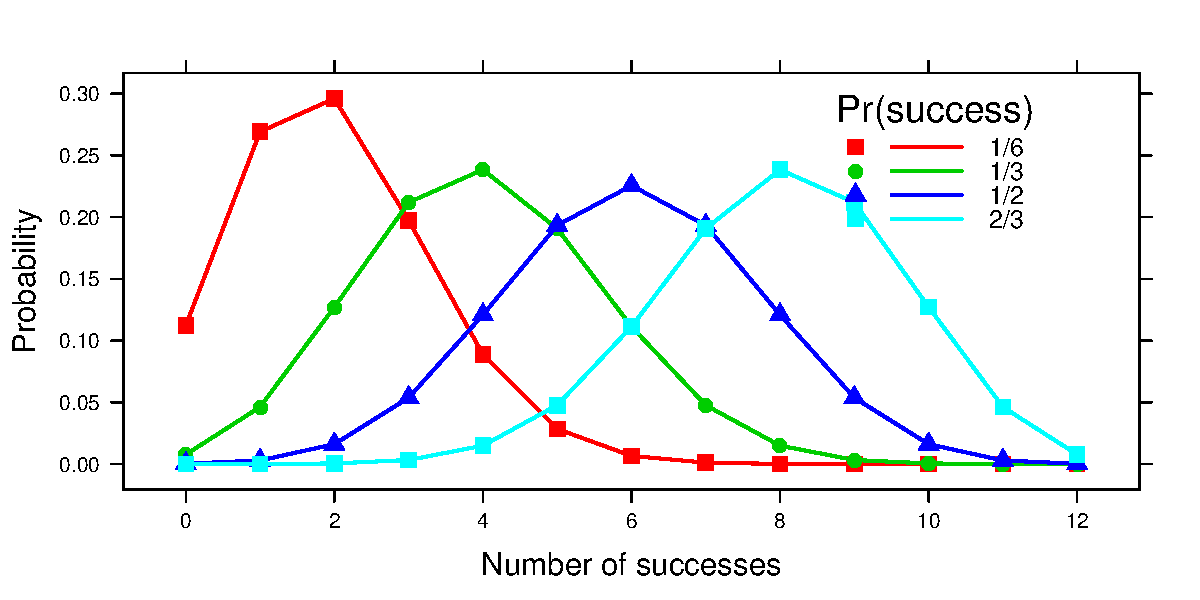
\includegraphics[width=.75\textwidth]{ch03/fig/dbinom2-plot} }

\caption[Binomial distributions for n=0--12 trials and four values of p]{Binomial distributions for n=0--12 trials and four values of p\label{fig:dbinom2-plot}}
\end{figure}


\end{knitrout}


\ix{binomial distribution|)}  % end index on

\subsection{The Poisson distribution}\label{sec:poisson}
\ix{Poisson distribution|(}

The Poisson distribution gives the probability of an event occurring
$k = 0, 1, 2, \dots$ times over a large number of independent ``trials'',
when the probability, $p$, that the event occurs on any one
trial (in time or space) is small and constant.
Hence, the Poisson distribution is usually applied to the study of
rare events such as highway accidents at a particular location,
deaths from horse kicks, or defects in a well-controlled manufacturing
process.  Other applications include:
the number of customers contacting a call center per unit time;
the number of insurance claims per unit region or unit time;
number of particles emitted from a small radioactive sample.

For the \IX{Poisson distribution}, the probability function
is
\begin{equation}\label{eq:poisf}
\Pois(\lambda):\Pr \{ X = k \} \equiv p (k)=
  \frac{ e^{ - \lambda } \:  \lambda^k } { k ! }
  \quad\quad k = 0, 1, \dots
\end{equation}
where the rate parameter, $\lambda$ ($>0$) turns out to be the mean of the
distribution.
The first three (central) moments of the Poisson distribution are:
%in fact all equal to $\lambda$:
\begin{eqnarray*}
\textrm{Mean}[X] & = & \lambda \\
\textrm{Var}[X] &  = & \lambda \\
\textrm{Skew}[X] & = & \lambda^{- 1/2} 
\end{eqnarray*}
%% Mathematica gives Skew = 1 / \sqrt(\lambda) ???

So, the mean and variance of the Poisson distribution are always
the same, which is sometimes used to identify a distribution
as Poisson.  For the binomial distribution, the mean ($Np$) is always
greater than the variance ($Npq$); for other distributions
(negative binomial and geometric) the mean is less than the
variance. The Poisson distribution is always positively skewed,
but skewness decreases as $\lambda$ increases.

The maximum likelihood estimator of the parameter \(\lambda\)
in \eqref{eq:poisf} is just
the mean of the distribution,
\begin{equation}
  \hat{\lambda}= \bar{x} = \frac{\sum_k k \,  n_k}{\sum_k  n_k} \label{eq:pois-lambda}
  \period
\end{equation}
Hence, the expected frequencies can be estimated by substituting the
sample mean into \eqref{eq:poisf} and multiplying by the total
sample size $N$.

There are many useful properties of the Poisson distribution.%
\footnote{
See: \url{http://en.wikipedia.org/wiki/Poisson_distribution}
}
Among these:
\begin{itemize*}
  \item Poisson variables have a nice reproductive property:
 if $X_1, X_2, \dots X_m$ are independent Poisson
variables with the same parameter $\lambda$, then their
sum, $\sum X_i$ is a Poisson variate with parameter $m \lambda$;
if the Poisson parameters differ, the sum is still Poisson with
parameter $\sum \lambda_i$.
  \item For two or more independent Poisson variables, 
  $X_1 \sim \Pois(\lambda_1),
  $X_2 \sim \Pois(\lambda_2), \dots$, with rate parameters 
  $ \lambda_1, \lambda_2 \dots$, the distribution of 
  any $X_i$ \emph{conditional on their sum}, $\sum_j X_j = k$ is
  binomial, $\Bin (k, p)$, where $p = \lambda_i / \sum_j \lambda_j$.
  \item As $\lambda$ increases, the Poisson distribution becomes increasingly
  symmetric, and approaches the normal distribution $N (\lambda, \lambda)$
  with mean and variance $\lambda$ as $\lambda \rightarrow \infty$.
  The approximation is quite good with $\lambda > 20$.
  \item If $X \sim \Pois(\lambda)$, then $\sqrt{X}$ converges much faster to
  a normal distribution $N (\lambda, \frac14)$, with mean $\sqrt\lambda}$
  and constant variance $\frac14$.  Hence, the square root transformation is often recommended
  as a \emph{variance stabilizing} transformation for count data 
  when classical methods (ANOVA, regression) assuming normality are employed.
\end{itemize*}


\begin{Example}[soccer]{UK Soccer scores}
\tabref{tab:soccer1}  gives the distributions of goals scored by
the 20 teams in the  1995/96 season of the
 Premier League of the UK Football Association
as presented originally by 
\citet{Lee:97}, and now available as the two-way table \data{UKSoccer}
in the \Rpackage{vcd}.
\begin{table}[htb]
\caption{Goals scored by home and away teams in 380 games in the Premier
Football League, 1995/96 season}
\label{tab:soccer1}
\begin{center}
\vspace{.1in}
\begin{tabular}{r|rrrrr|r}
  \hline
Home      & \multicolumn{5}{c|}{Away Team Goals} \\
Team      &       0 &      1 &       2&       3&      4+&  Total \\
Goals     &  \multicolumn{5}{c|}{}   \\
  \hline
			0 &     27 &     29 &     10 &      8 &      2 &     76 \\
			1 &     59 &     53 &     14 &     12 &      4 &    142 \\
			2 &     28 &     32 &     14 &     12 &      4 &     90 \\
			3 &     19 &     14 &      7 &      4 &      1 &     45 \\
			4+&      7 &      8 &     10 &      2 &      0 &     27 \\
  \hline
Total      &  140   &    136 &     55 &     38 &     11 &    380 \\
  \hline
\end{tabular}
\end{center}
\end{table}
Over a season
each team plays each other team exactly once, so there are a total of
$20 \times 19 = 380$ games.
Because there may be an advantage for the home team,
the goals scored have been classified as ``home team'' goals
and ``away team'' goals in the table. Of interest for this example is whether
the number of goals scores by home teams and away teams follow
Poisson distributions, and how this relates to the distribution of the 
total number of goals scored.

If we assume that in any small interval of time there is a small, constant
probability that the home team or the away team may score a goal,
the distributions of the goals scored by home teams
(the row totals in \tabref{tab:soccer1})
may be modeled as Pois($\lambda_H$) and the distribution of
the goals scored by away teams (the column totals)
may be modeled as Pois($\lambda_A$).

If the number of goals scored by the home and away teams are independent%
\footnote{This question
is examined visually in \chref{ch:mosaic} (\exref{ex:soccer2})
and \chref{ch:corresp} (\exref{ex:soccer3}), where we find that the answer
is ``basically, yes''.},
we would expect that the total number of goals scored in any
game would be distributed as Pois($\lambda_H + \lambda_A$).
These totals are shown in \tabref{tab:soccer2}.
\begin{table}[!hb]
\caption{Total goals scored in 380 games in the Premier
Football League, 1995/95 season}
\label{tab:soccer2}
\vspace{.1in}
\begin{center}
\begin{tabular}{l|rrrr rrrr}
\hline
Total goals      &  0  &  1  &  2  &  3  &  4  &  5  &  6  &  7  \\
\hline
Number of games  & 27  & 88  & 91  & 73  & 49  & 31  & 18  &  3  \\
  \hline
\end{tabular}
\end{center}
\end{table}


As preliminary check of the distributions for the home and away goals,
we can determine if the means and variances are reasonably close
to each other.
If so, then the total goals variable should also have a mean and variance
equal to the sum of those statistics for the home and away goals.

In the \R code below, we first convert the two-way frequency table
\data{UKSoccer} to a data frame in frequency form.
We use \func{within} to convert \var{Home} and \var{Away} to
numeric variables, and calculate \var{Total} as their sum.

\begin{knitrout}
\definecolor{shadecolor}{rgb}{0.969, 0.969, 0.969}\color{fgcolor}\begin{kframe}
\begin{alltt}
\hlkwd{data}\hlstd{(UKSoccer,} \hlkwc{package}\hlstd{=}\hlstr{"vcd"}\hlstd{)}

\hlstd{soccer.df} \hlkwb{<-} \hlkwd{as.data.frame}\hlstd{(UKSoccer,} \hlkwc{stringsAsFactors}\hlstd{=}\hlnum{FALSE}\hlstd{)}
\hlstd{soccer.df} \hlkwb{<-} \hlkwd{within}\hlstd{(soccer.df,}
  \hlstd{\{}
  \hlstd{Home} \hlkwb{<-} \hlkwd{as.numeric}\hlstd{(Home)}          \hlcom{# make numeric}
  \hlstd{Away} \hlkwb{<-} \hlkwd{as.numeric}\hlstd{(Away)}          \hlcom{# make numeric}
  \hlstd{Total} \hlkwb{<-} \hlstd{Home} \hlopt{+} \hlstd{Away}              \hlcom{# total goals}
  \hlstd{\})}
\hlkwd{str}\hlstd{(soccer.df)}
\end{alltt}
\begin{verbatim}
## 'data.frame':	25 obs. of  4 variables:
##  $ Home : num  0 1 2 3 4 0 1 2 3 4 ...
##  $ Away : num  0 0 0 0 0 1 1 1 1 1 ...
##  $ Freq : num  27 59 28 19 7 29 53 32 14 8 ...
##  $ Total: num  0 1 2 3 4 1 2 3 4 5 ...
\end{verbatim}
\end{kframe}
\end{knitrout}

To calculate the mean and variance of these variables, first expand
the data frame to 380 individual observations using \func{expand.dft}.
Then use \func{apply} over the rows to calculate the mean and variance
in each column.
\begin{knitrout}
\definecolor{shadecolor}{rgb}{0.969, 0.969, 0.969}\color{fgcolor}\begin{kframe}
\begin{alltt}
\hlstd{soccer.df} \hlkwb{<-} \hlkwd{expand.dft}\hlstd{(soccer.df)}   \hlcom{# expand to ungrouped form}
\hlkwd{apply}\hlstd{(soccer.df,} \hlnum{2}\hlstd{,} \hlkwc{FUN}\hlstd{=}\hlkwa{function}\hlstd{(}\hlkwc{x}\hlstd{)} \hlkwd{c}\hlstd{(}\hlkwc{mean}\hlstd{=}\hlkwd{mean}\hlstd{(x),} \hlkwc{var}\hlstd{=}\hlkwd{var}\hlstd{(x)))}
\end{alltt}
\begin{verbatim}
##       Home  Away Total
## mean 1.487 1.063 2.550
## var  1.316 1.173 2.618
\end{verbatim}
\end{kframe}
\end{knitrout}


The means are all approximately equal to the corresponding variances.
More to the point, the variance of the \texttt{Total} score
is approximately equal to the sum of the individual variances.
Note also there does appear to be an advantage for the home team,
of nearly half a goal.

\end{Example}

\begin{Example}[cyclists2]{London cycling deaths}
A quick check of whether the numbers of deaths among London cyclists
follows the Poisson distribution
can be carried out by calculating the mean and variance.
The \term{index of dispersion}, the ratio of the variance to the mean,
is commonly used to quantify whether a set of observed frequencies 
is more or less dispersed than a reference (Poisson) distribution.
\begin{knitrout}
\definecolor{shadecolor}{rgb}{0.969, 0.969, 0.969}\color{fgcolor}\begin{kframe}
\begin{alltt}
\hlstd{(mean} \hlkwb{<-} \hlkwd{mean}\hlstd{(CyclingDeaths}\hlopt{$}\hlstd{deaths))}
\end{alltt}
\begin{verbatim}
## [1] 0.5673
\end{verbatim}
\begin{alltt}
\hlstd{(var} \hlkwb{<-} \hlkwd{var}\hlstd{(CyclingDeaths}\hlopt{$}\hlstd{deaths))}
\end{alltt}
\begin{verbatim}
## [1] 0.5268
\end{verbatim}
\begin{alltt}
\hlstd{var}\hlopt{/}\hlstd{mean}
\end{alltt}
\begin{verbatim}
## [1] 0.9287
\end{verbatim}
\end{kframe}
\end{knitrout}

Thus, there was an average of 0.57 deaths per fortnight,
or a bit more than 1 per month, and no evidence for over- or under-
dispersion.

We can now answer the question of whether it was an extraordinay
event to observe six deaths in a two-week period, by calculating
the probability of more than 5 deaths using \func{ppois}.
\begin{knitrout}
\definecolor{shadecolor}{rgb}{0.969, 0.969, 0.969}\color{fgcolor}\begin{kframe}
\begin{alltt}
\hlnum{1} \hlopt{-} \hlkwd{ppois}\hlstd{(}\hlnum{5}\hlstd{, mean)}
\end{alltt}
\begin{verbatim}
## [1] 2.854e-05
\end{verbatim}
\begin{alltt}
\hlkwd{ppois}\hlstd{(}\hlnum{5}\hlstd{, mean,} \hlkwc{lower.tail}\hlstd{=}\hlnum{FALSE}\hlstd{)}
\end{alltt}
\begin{verbatim}
## [1] 2.854e-05
\end{verbatim}
\end{kframe}
\end{knitrout}

This probability is extremely small, so we conclude that the
occurrence of six deaths was a singular event.
The interpretation of this result might indicate an increased
risk to cycling in London, and might prompt further study of
road safety.  
\end{Example}


\subsubsection{Calculation and visualization}
For the Poisson distribution, you can generate probabilities using
\code{dpois(x, lambda)} for the numbers of events in \code{x} with
rate parameter \code{lambda}. As we did earlier for the binomial 
distribution, we can calculate these for a collection of values
of \code{lambda} by using \func{expand.grid} to create all combinations
of with the values of \code{x} we wish to plot.

\begin{Example}[dpois-plot]{Plotting styles for discrete distributions}
In this example, we illustrate some additional styles for plotting discrete
distributions, using both \pkg{lattice} \func{xyplot} and the
\Rpackage{ggplot2}.  The goal here is to visualize a collection of
Poisson distributions for varying values of $\lambda$.

We first create the 63 combinations of \code{x=0:20} for
three values of $\lambda$, \code{lambda=c(1, 4, 10)}, and use these
columns as arguments to \func{dpois}.  Again, \code{lambda} is
a numeric variable, but the plotting methods are easier if this
variable is converted to a factor.
\begin{knitrout}
\definecolor{shadecolor}{rgb}{0.969, 0.969, 0.969}\color{fgcolor}\begin{kframe}
\begin{alltt}
\hlstd{XL} \hlkwb{<-}\hlkwd{expand.grid}\hlstd{(}\hlkwc{x}\hlstd{=}\hlnum{0}\hlopt{:}\hlnum{20}\hlstd{,} \hlkwc{lambda}\hlstd{=}\hlkwd{c}\hlstd{(}\hlnum{1}\hlstd{,} \hlnum{4}\hlstd{,} \hlnum{10}\hlstd{))}
\hlstd{pois.df} \hlkwb{<-} \hlkwd{data.frame}\hlstd{(XL,} \hlkwc{prob}\hlstd{=}\hlkwd{dpois}\hlstd{(XL[,}\hlstr{"x"}\hlstd{], XL[,}\hlstr{"lambda"}\hlstd{]))}
\hlstd{pois.df}\hlopt{$}\hlstd{lambda} \hlkwb{=} \hlkwd{factor}\hlstd{(pois.df}\hlopt{$}\hlstd{lambda)}
\hlkwd{str}\hlstd{(pois.df)}
\end{alltt}
\begin{verbatim}
## 'data.frame':	63 obs. of  3 variables:
##  $ x     : int  0 1 2 3 4 5 6 7 8 9 ...
##  $ lambda: Factor w/ 3 levels "1","4","10": 1 1 1 1 1 1 1 1 1 1 ...
##  $ prob  : num  0.3679 0.3679 0.1839 0.0613 0.0153 ...
\end{verbatim}
\end{kframe}
\end{knitrout}


Discrete distributions are often plotted as bar charts or in histogram-like
form, as we did for the examples in \secref{sec:discrete-intro},
rather than the line-graph form used for the binomial distribution in 
\figref{fig:dbinom2-plot}.  With \func{xyplot}, the plot style is controlled
by the \code{type} argument, and the code below uses \code{type=c("h", "p")}
to get \emph{both} histogram-like lines to the origin and points.
As well, the plot formula, \code{prob ~ x | lambda} instructs \func{xyplot}
to produce a multi-panel plot, conditioned on values of \code{lambda}.
These lines produce \figref{fig:dpois-xyplot1}.

\begin{knitrout}
\definecolor{shadecolor}{rgb}{0.969, 0.969, 0.969}\color{fgcolor}\begin{kframe}
\begin{alltt}
\hlkwd{xyplot}\hlstd{( prob} \hlopt{~} \hlstd{x} \hlopt{|} \hlstd{lambda,} \hlkwc{data}\hlstd{=pois.df,}
  \hlkwc{type}\hlstd{=}\hlkwd{c}\hlstd{(}\hlstr{"h"}\hlstd{,} \hlstr{"p"}\hlstd{),} \hlkwc{pch}\hlstd{=}\hlnum{16}\hlstd{,} \hlkwc{lwd}\hlstd{=}\hlnum{4}\hlstd{,} \hlkwc{cex}\hlstd{=}\hlnum{1.25}\hlstd{,} \hlkwc{layout}\hlstd{=}\hlkwd{c}\hlstd{(}\hlnum{3}\hlstd{,}\hlnum{1}\hlstd{),}
  \hlkwc{xlab}\hlstd{=}\hlkwd{list}\hlstd{(}\hlstr{"Number of events (k)"}\hlstd{,} \hlkwc{cex}\hlstd{=}\hlnum{1.25}\hlstd{),}
  \hlkwc{ylab}\hlstd{=}\hlkwd{list}\hlstd{(}\hlstr{"Probability"}\hlstd{,}  \hlkwc{cex}\hlstd{=}\hlnum{1.25}\hlstd{))}
\end{alltt}
\end{kframe}\begin{figure}[htbp]


\centerline{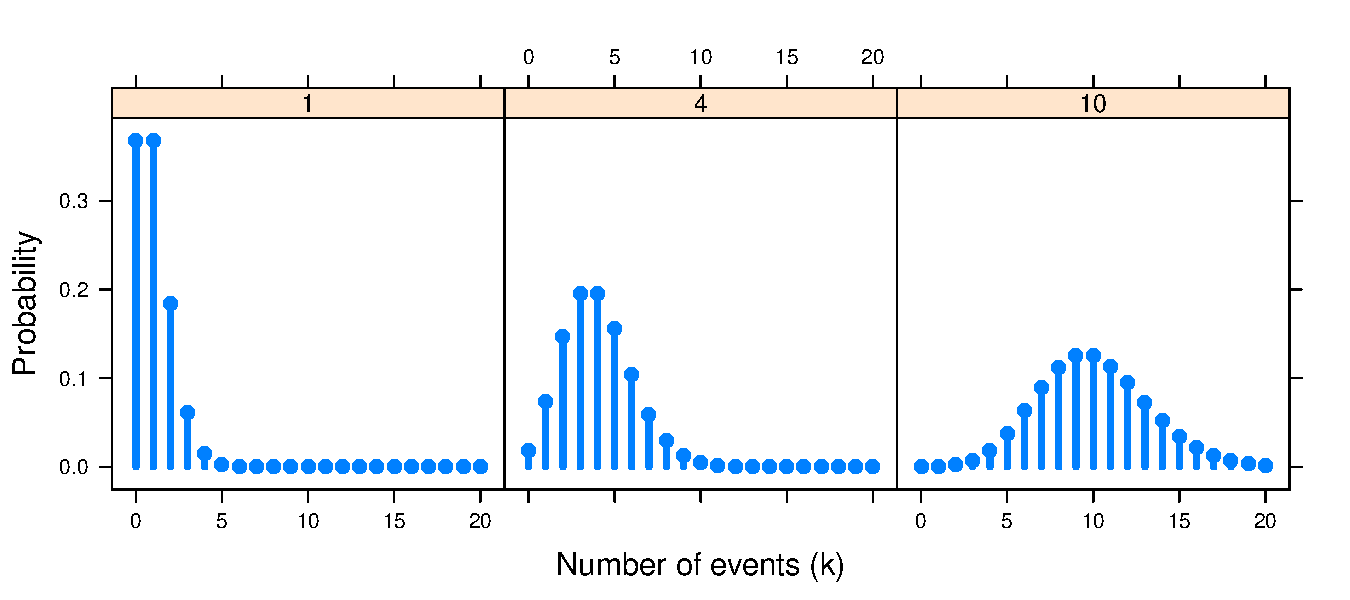
\includegraphics[width=\textwidth]{ch03/fig/dpois-xyplot1} }

\caption[Poisson distributions for $\lambda$ = 1, 4, 10, in a multi-panel display]{Poisson distributions for $\lambda$ = 1, 4, 10, in a multi-panel display\label{fig:dpois-xyplot1}}
\end{figure}


\end{knitrout}


The line-graph plot style of \figref{fig:dbinom2-plot} has the advantage that
it is easier to compare the separate distributions in a single plot 
(using the \code{groups} argument) than
across multiple panels (using a conditioning formula). 
It has the disadvantages that (a) a proper legend is
difficult to construct with \pkg{lattice}, and (b) is difficult to read, because
you have to visually coordinate the curves in the plot with the values shown
in the legend.  \figref{fig:dpois-xyplot2} solves both problems using
the \Rpackage{directlabels}.
\begin{knitrout}
\definecolor{shadecolor}{rgb}{0.969, 0.969, 0.969}\color{fgcolor}\begin{kframe}
\begin{alltt}
\hlstd{mycol} \hlkwb{<-} \hlkwd{palette}\hlstd{()[}\hlnum{2}\hlopt{:}\hlnum{4}\hlstd{]}
\hlstd{plt} \hlkwb{<-} \hlkwd{xyplot}\hlstd{( prob} \hlopt{~} \hlstd{x,} \hlkwc{data}\hlstd{=pois.df,} \hlkwc{groups}\hlstd{=lambda,}
  \hlkwc{type}\hlstd{=}\hlstr{"b"}\hlstd{,} \hlkwc{pch}\hlstd{=}\hlnum{15}\hlopt{:}\hlnum{17}\hlstd{,} \hlkwc{lwd}\hlstd{=}\hlnum{2}\hlstd{,} \hlkwc{cex}\hlstd{=}\hlnum{1.25}\hlstd{,} \hlkwc{col}\hlstd{=mycol,}
  \hlkwc{xlab}\hlstd{=}\hlkwd{list}\hlstd{(}\hlstr{"Number of events (k)"}\hlstd{,} \hlkwc{cex}\hlstd{=}\hlnum{1.25}\hlstd{),}
        \hlkwc{ylab}\hlstd{=}\hlkwd{list}\hlstd{(}\hlstr{"Probability"}\hlstd{,}  \hlkwc{cex}\hlstd{=}\hlnum{1.25}\hlstd{))}

\hlkwd{library}\hlstd{(directlabels)}
\hlkwd{direct.label}\hlstd{(plt,} \hlkwd{list}\hlstd{(}\hlstr{"top.points"}\hlstd{,} \hlkwc{cex}\hlstd{=}\hlnum{1.5}\hlstd{,} \hlkwd{dl.trans}\hlstd{(}\hlkwc{y}\hlstd{=y}\hlopt{+}\hlnum{0.1}\hlstd{)))}
\end{alltt}
\end{kframe}\begin{figure}[htbp]


\centerline{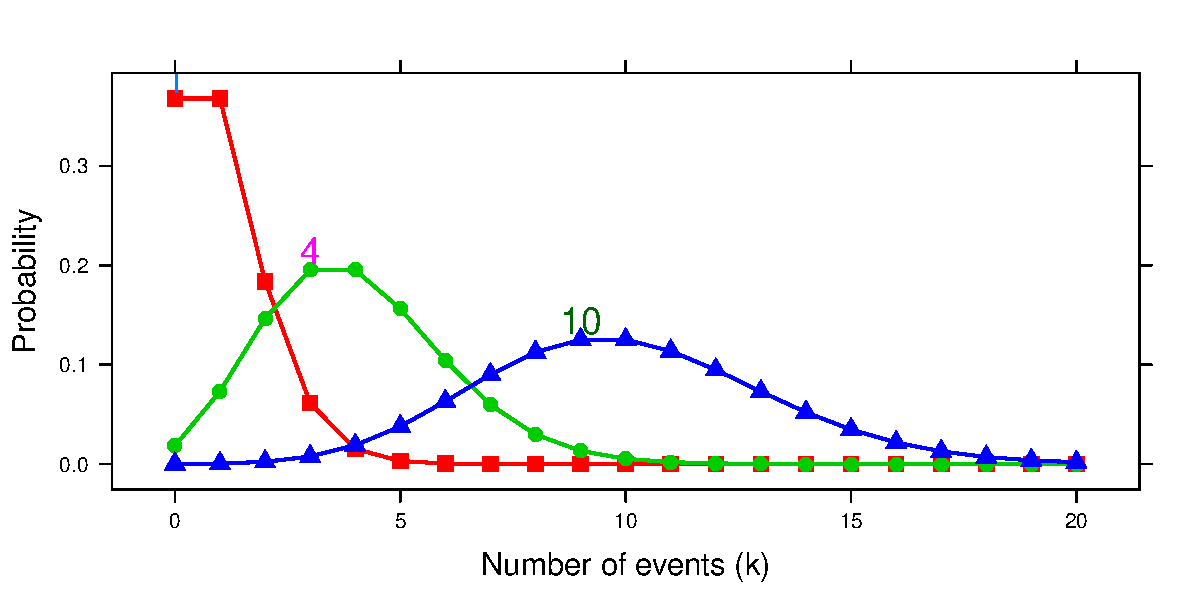
\includegraphics[width=.8\textwidth]{ch03/fig/dpois-xyplot2} }

\caption[Poisson distributions for $\lambda$ = 1, 4, 10, using direct labels]{Poisson distributions for $\lambda$ = 1, 4, 10, using direct labels\label{fig:dpois-xyplot2}}
\end{figure}


\end{knitrout}

Note that the plot constructed by \func{xyplot} is saved as a
(\class{trellis}) object, \code{plt}.  The function
\func{direct.label} 
massages this to add the labels directly to each curve.  In the
second argument above, \code{"top.points"} says to locate these
at the maximum value on each curve.

Finally, we illustrate the use of \pkg{ggplot2} to produce a single-panel,
multi-line plot of these distributions. The basic plot uses
\code{aes(x=x, y=prob, ...)} to produce a plot of \code{prob} vs. \code{x},
assigning color and shape attributes to the values of \code{lambda}.

\begin{knitrout}
\definecolor{shadecolor}{rgb}{0.969, 0.969, 0.969}\color{fgcolor}\begin{kframe}
\begin{alltt}
\hlkwd{library}\hlstd{(ggplot2)}
\hlstd{gplt} \hlkwb{<-} \hlkwd{ggplot}\hlstd{(pois.df,} \hlkwd{aes}\hlstd{(}\hlkwc{x}\hlstd{=x,} \hlkwc{y}\hlstd{=prob,} \hlkwc{colour}\hlstd{=lambda,} \hlkwc{shape}\hlstd{=lambda))} \hlopt{+}
  \hlkwd{geom_line}\hlstd{(}\hlkwc{size}\hlstd{=}\hlnum{1}\hlstd{)} \hlopt{+} \hlkwd{geom_point}\hlstd{(}\hlkwc{size}\hlstd{=}\hlnum{3}\hlstd{)} \hlopt{+}
        \hlkwd{xlab}\hlstd{(}\hlstr{"Number of events (k)"}\hlstd{)} \hlopt{+}
        \hlkwd{ylab}\hlstd{(}\hlstr{"Probability"}\hlstd{)}
\end{alltt}
\end{kframe}
\end{knitrout}

\pkg{ggplot2} allows most details of the plot to be modified using
\func{theme}.  Here we use this to move the legend inside the plot,
and enlarge the axis labels and titles.
\begin{knitrout}
\definecolor{shadecolor}{rgb}{0.969, 0.969, 0.969}\color{fgcolor}\begin{kframe}
\begin{alltt}
\hlstd{gplt} \hlopt{+} \hlkwd{theme}\hlstd{(}\hlkwc{legend.position}\hlstd{=}\hlkwd{c}\hlstd{(}\hlnum{0.8}\hlstd{,}\hlnum{0.8}\hlstd{))} \hlopt{+}  \hlcom{# manually move legend}
       \hlkwd{theme}\hlstd{(}\hlkwc{axis.text}\hlstd{=}\hlkwd{element_text}\hlstd{(}\hlkwc{size}\hlstd{=}\hlnum{12}\hlstd{),}
            \hlkwc{axis.title}\hlstd{=}\hlkwd{element_text}\hlstd{(}\hlkwc{size}\hlstd{=}\hlnum{14}\hlstd{,}\hlkwc{face}\hlstd{=}\hlstr{"bold"}\hlstd{))}
\end{alltt}
\end{kframe}\begin{figure}[htbp]


\centerline{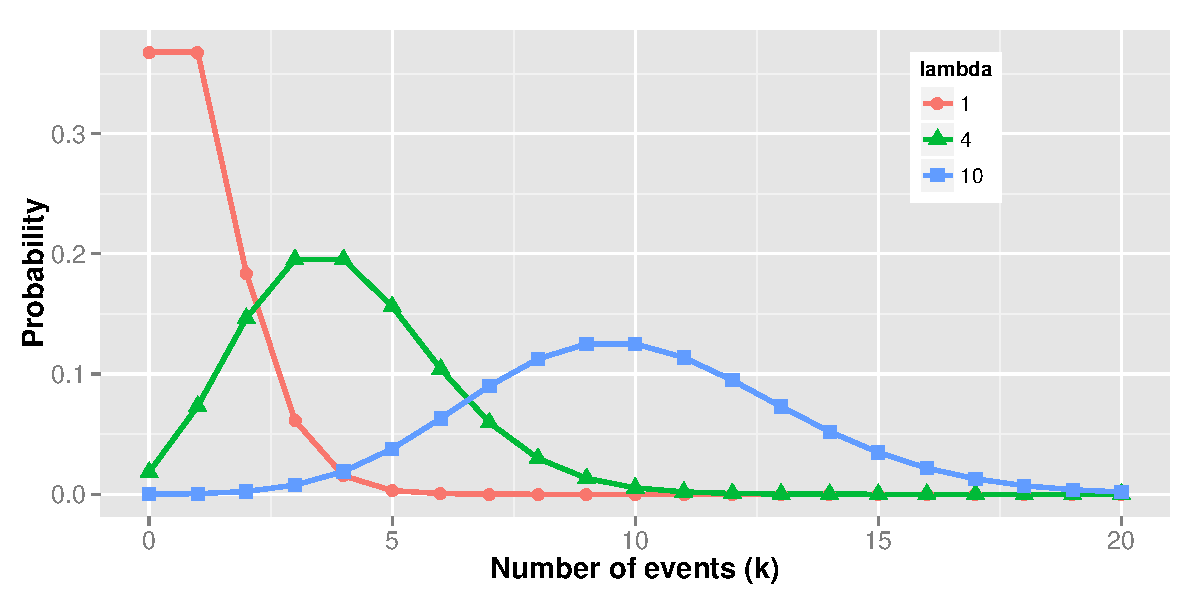
\includegraphics[width=.8\textwidth]{ch03/fig/dpois-ggplot2} }

\caption[Poisson distributions for $\lambda$ = 1, 4, 10, using ggplot]{Poisson distributions for $\lambda$ = 1, 4, 10, using ggplot\label{fig:dpois-ggplot2}}
\end{figure}


\end{knitrout}


\end{Example}

\ix{Poisson distribution|)}

\subsection{The negative binomial distribution}\label{sec:negbin}
\ix{negative binomial distribution|(}

The negative binomial distribution is a type of waiting-time distribution,
but also arises in statistical applications as a generalization of the
Poisson distribution, allowing for \term{overdispersion} (variance > mean).
See \citet{Hilbe:2011:negbin} for a comprehensive treatment 
of negative binomial statistical models with many applications in \R.

One form of
the negative binomial distribution
(also called the \term{Pascal distribution}) arises when a series of 
independent Bernoulli
trials is observed with constant probability $p$ of some event,
and we ask how many non-events (failures), $k$, it takes to observe
$n$ successful events.  For example, in tossing one die repeatedly, 
we may consider the outcome ``1'' as a ``success'' (with $p=\frac16$) 
and ask about the probability of observing $k = 0, 1, 2, \dots$
failures before getting $n=3$ 1s.


The probability function with parameters $n$ (a positive integer, $0 < n < \infty$) and $p \, (0 < p < 1)$
gives the probability that $k$ non-events (failures) are observed before
the $n$-th event (success), and
can be written%
\footnote{
There are a variety of other parameterizations of the negative binomial distribution,
but all of these can be converted to the form shown here, which is relatively
standard, and consistent with \R. They differ in whether the parameter $n$
relates to the the number of successes or the total number of trials, and
whether the stopping criterion is defined in terms of failures or successes.
See: \url{http://en.wikipedia.org/wiki/Negative_binomial_distribution}
for details on these variations.
}
\begin{equation}\label{eq:negbinf}
\NBin(n,p):   \Pr \{ X = k \} \equiv p(k)  =
  {n+k-1 \choose k} p^n (1-p)^k
  \quad\quad k = 0, 1, \dots , \infty
\end{equation}
This formulation makes clear that a given sequence of events involves 
a total of $n+k$ trials of which there are $n$ successes,
with probability $p^n$, and $k$ are failures, with probability $(1-p)^k$.
The binomial coefficient, ${n+k-1 \choose k}$ gives the number of ways
to choose the $k$ successes from the remaining $n+k-1$ trials preceding
the last success.

The first three central moments of the negative binomial distribution are:
\begin{eqnarray*}
\textrm{Mean}[X] &=&nq / p  = \mu \\
\textrm{Var}[X] &=&nq / p^2 \\
\textrm{Skew}[X] &=&\frac{2-p}{\sqrt{nq}}
\comma
\end{eqnarray*}
where $q=1-p$. The variance of $X$ is therefore greater than the mean,
and the distribution is always positively skewed.

A more general form of the negative binomial distribution 
(the \term{Polya distribution})
allows $n$ to take non-integer values and to be an unknown
parameter.
In this case, the combinatorial coefficient,
${n+k-1 \choose k}$ in \eqref{eq:negbinf} is calculated using
the gamma function, $\Gamma(\bullet)$,
a generalization of the factorial for non-integer values,
defined so that $\Gamma(x+1) = x!$ when $x$ is an integer.

Then the probability function \eqref{eq:negbinf} becomes
\begin{equation}\label{eq:negbinf2}
  \Pr \{ X = k \} \equiv p(k)  =
  \frac{\Gamma(n+k)}{\Gamma(n) \Gamma(k+1)}
   p^n (1-p)^k
  \quad\quad k = 0, 1, \dots , \infty
  \period
\end{equation}

\citet{GreenwoodYule:20}
developed the negative binomial distribution as a model for
accident proneness or susceptibility of individuals to
repeated attacks of disease.
They assumed that for any individual, $i$, the number of accidents
or disease occurrences has a Poisson distribution with parameter
$\lambda_i$.
If individuals vary in proneness, so that the $\lambda_i$ have
a gamma distribution, the resulting distribution is the
negative binomial.

In this form, the negative binomial distribution is frequently used
as an alternative to the Poisson distribution when the assumptions
of the Poisson (constant probability and independence) are not
satisfied, or when the variance of the distribution is greater
than the mean (overdispersion).
This gives rise to an alternative parameterization in terms of the
mean ($\mu$) of the distribution and its relation to the variance.
From the relation of the mean and variance to the parameters
$n, p$ given above,

\begin{eqnarray}
\textrm{Mean}[X] = \mu = \frac{n (1-p)}{p} & \implies & p = \frac{n}{n+\mu} \\
\textrm{Var}[X] = \frac{n (1-p)}{p^2} & \implies & \textrm{Var}[X] = \mu + \frac{\mu^2}{n}
\end{eqnarray}}
This formulation allows the variance of the distribution to exceed the mean,
and in these terms, the ``size'' parameter $n$ is called the the
\term{dispersion parameter}.%
\footnote{
Other terms are ``shape parameter,'' with reference to the mixing distribution
of Poissons with varying $\lambda$, 
``heterogeneity parameter,'' or ``aggregation parameter.''
}
Increasing this parameter corresponds to less heterogeneity, variance closer
to the mean, and therefore greater applicability of the Poisson distribution.

\subsubsection{Calculation and visualization}

In \R, the density (pmf), distribution (CDF), quantile and random number functions
for the negative binomial distribution are a bit special, in that the parameterization
can be specified using either $(n, p)$ or $(n, \mu)$ forms,
where $\mu = n (1-p) /p$.
In our notation, probabilities can be calculated using \func{dnbinom}
using the call \code{dbinom(k, n, p)}
or the call \code{dbinom(k, n, mu=)}, as illustrated below:

\begin{knitrout}
\definecolor{shadecolor}{rgb}{0.969, 0.969, 0.969}\color{fgcolor}\begin{kframe}
\begin{alltt}
\hlstd{k} \hlkwb{=} \hlnum{2}
\hlstd{n} \hlkwb{=} \hlnum{2}\hlopt{:}\hlnum{4}
\hlstd{p} \hlkwb{=} \hlnum{.2}
\hlkwd{dnbinom}\hlstd{( k, n,  p)}
\end{alltt}
\begin{verbatim}
## [1] 0.07680 0.03072 0.01024
\end{verbatim}
\begin{alltt}
\hlstd{mu} \hlkwb{=} \hlstd{n}\hlopt{*}\hlstd{(}\hlnum{1}\hlopt{-}\hlstd{p)}\hlopt{/}\hlstd{p}
\hlstd{mu}
\end{alltt}
\begin{verbatim}
## [1]  8 12 16
\end{verbatim}
\begin{alltt}
\hlkwd{dnbinom}\hlstd{( k, n,} \hlkwc{mu}\hlstd{=mu)}
\end{alltt}
\begin{verbatim}
## [1] 0.07680 0.03072 0.01024
\end{verbatim}
\end{kframe}
\end{knitrout}

Thus, for the distribution with \code{k=2} failures and
 \code{n=2:4} successes with probability \code{p=0.2},
the values \code{n=2:4} correspond to means $\mu= 8, 12, 16$
as shown above.

As before, we can calculate these probabilities for a range
of the combinations of arguments using \func{expand.grid}.
In the example below,
we allow three values for each of \code{n} and \code{p}
and calculate all probabilities for all values of \code{k}
from 0 to 20. The result, \code{nbin.df} is like a 3-way,
$21 \times 3 \times 3$
array of \code{prob} values, but in data frame format.
\begin{knitrout}
\definecolor{shadecolor}{rgb}{0.969, 0.969, 0.969}\color{fgcolor}\begin{kframe}
\begin{alltt}
\hlstd{XN} \hlkwb{<-}\hlkwd{expand.grid}\hlstd{(}\hlkwc{k}\hlstd{=}\hlnum{0}\hlopt{:}\hlnum{20}\hlstd{,} \hlkwc{n}\hlstd{=}\hlkwd{c}\hlstd{(}\hlnum{2}\hlstd{,} \hlnum{4}\hlstd{,} \hlnum{6}\hlstd{),} \hlkwc{p}\hlstd{=}\hlkwd{c}\hlstd{(}\hlnum{0.2}\hlstd{,} \hlnum{0.3}\hlstd{,} \hlnum{0.4}\hlstd{))}
\hlstd{nbin.df} \hlkwb{<-} \hlkwd{data.frame}\hlstd{(XN,} \hlkwc{prob}\hlstd{=}\hlkwd{dnbinom}\hlstd{(XN[,}\hlstr{"k"}\hlstd{], XN[,}\hlstr{"n"}\hlstd{], XN[,}\hlstr{"p"}\hlstd{]))}
\hlstd{nbin.df}\hlopt{$}\hlstd{n} \hlkwb{=} \hlkwd{factor}\hlstd{(nbin.df}\hlopt{$}\hlstd{n)}
\hlstd{nbin.df}\hlopt{$}\hlstd{p} \hlkwb{=} \hlkwd{factor}\hlstd{(nbin.df}\hlopt{$}\hlstd{p)}
\hlkwd{str}\hlstd{(nbin.df)}
\end{alltt}
\begin{verbatim}
## 'data.frame':	189 obs. of  4 variables:
##  $ k   : int  0 1 2 3 4 5 6 7 8 9 ...
##  $ n   : Factor w/ 3 levels "2","4","6": 1 1 1 1 1 1 1 1 1 1 ...
##  $ p   : Factor w/ 3 levels "0.2","0.3","0.4": 1 1 1 1 1 1 1 1 1 1 ...
##  $ prob: num  0.04 0.064 0.0768 0.0819 0.0819 ...
\end{verbatim}
\end{kframe}
\end{knitrout}


With 9 combinations of the parameters, it is most convenient
to plot these in separate panels, in a $3 \times 3$ display.
The formula \code{prob ~ k | n + p} in the call to
\func{xyplot} constructs plots of
\code{prob} vs. \code{k} conditioned on the combinations of
\code{n} and \code{p}.
\begin{knitrout}
\definecolor{shadecolor}{rgb}{0.969, 0.969, 0.969}\color{fgcolor}\begin{kframe}
\begin{alltt}
\hlkwd{xyplot}\hlstd{( prob} \hlopt{~} \hlstd{k} \hlopt{|} \hlstd{n} \hlopt{+} \hlstd{p,} \hlkwc{data}\hlstd{=nbin.df,}
  \hlkwc{xlab}\hlstd{=}\hlkwd{list}\hlstd{(}\hlstr{'Number of failures (k)'}\hlstd{,} \hlkwc{cex}\hlstd{=}\hlnum{1.25}\hlstd{),}
  \hlkwc{ylab}\hlstd{=}\hlkwd{list}\hlstd{(}\hlstr{'Probability'}\hlstd{,}  \hlkwc{cex}\hlstd{=}\hlnum{1.25}\hlstd{),}
  \hlkwc{type}\hlstd{=}\hlkwd{c}\hlstd{(}\hlstr{'h'}\hlstd{,} \hlstr{'p'}\hlstd{),} \hlkwc{pch}\hlstd{=}\hlnum{16}\hlstd{,} \hlkwc{lwd}\hlstd{=}\hlnum{2}\hlstd{,}
  \hlkwc{strip} \hlstd{=} \hlkwd{strip.custom}\hlstd{(}\hlkwc{strip.names}\hlstd{=}\hlnum{TRUE}\hlstd{)}
        \hlstd{)}
\end{alltt}
\end{kframe}\begin{figure}[htbp]


\centerline{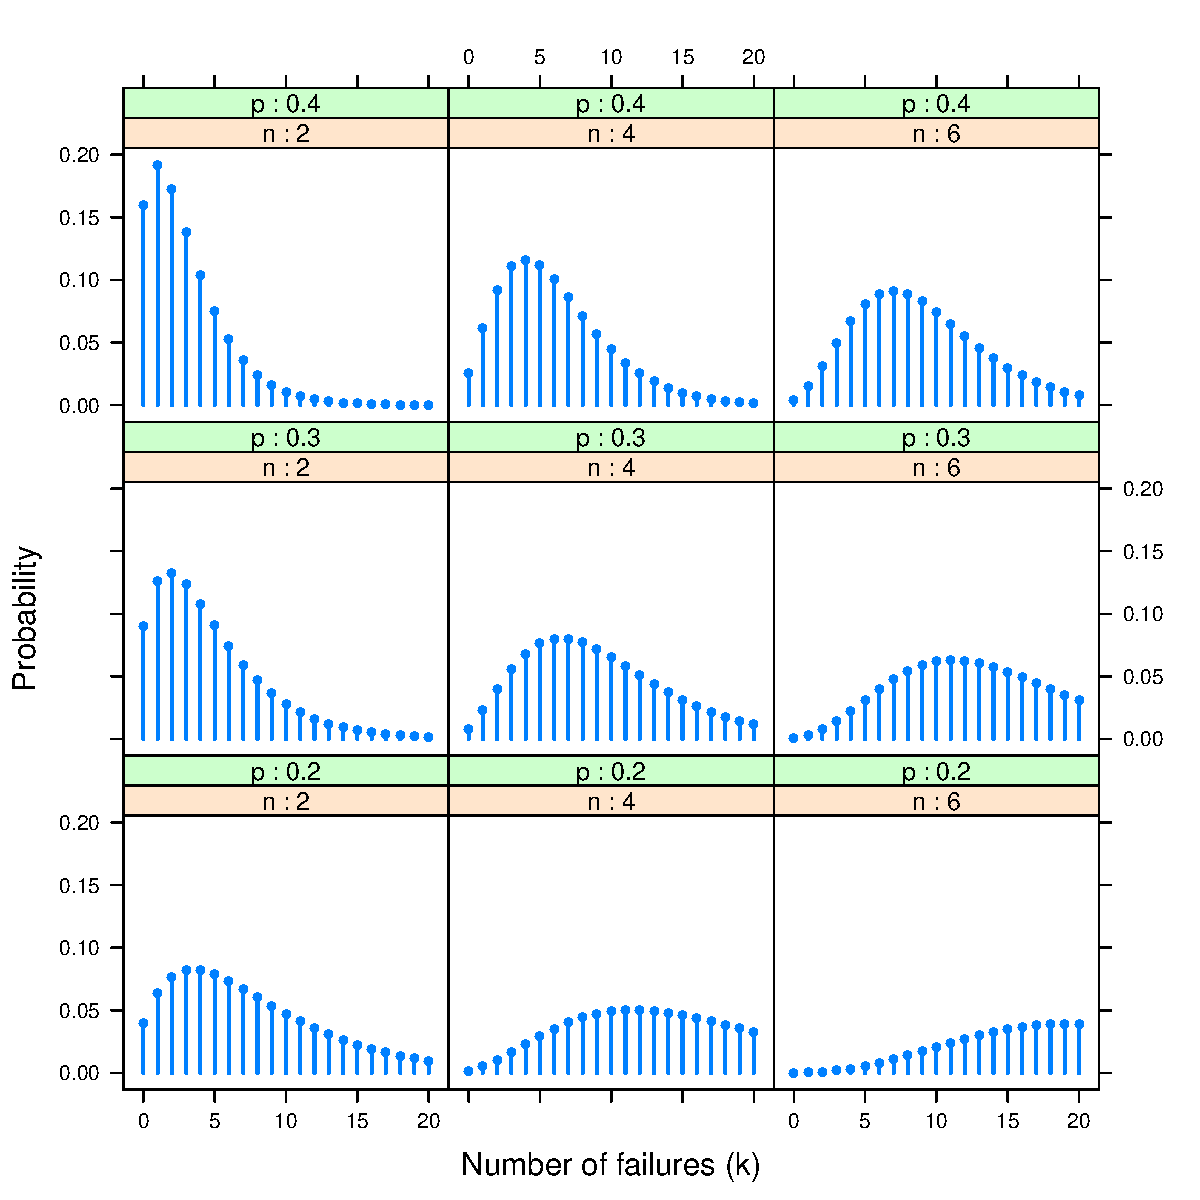
\includegraphics[width=.85\textwidth]{ch03/fig/dnbin3} }

\caption[Negative binomial distributions for $n = 2, 4, 6$ and $p=0]{Negative binomial distributions for $n = 2, 4, 6$ and $p=0.2, 0.3, 0.4$, using xyplot\label{fig:dnbin3}}
\end{figure}


\end{knitrout}

\TODO{Modify \figref{fig:dnbin3} to show the mean and standard deviation}

It can be readily seen that the mean increases from left to
right with \code{n}, and increases from top to bottom with
decreasing \code{p}.  For these distributions, we can also
calculate the theory-implied means, $\mu$, across the entire
distributions, $k = 0, 1, \dots \infty$, as shown below.

\begin{knitrout}
\definecolor{shadecolor}{rgb}{0.969, 0.969, 0.969}\color{fgcolor}\begin{kframe}
\begin{alltt}
\hlstd{NP} \hlkwb{<-} \hlkwd{expand.grid}\hlstd{(}\hlkwc{n}\hlstd{=}\hlkwd{c}\hlstd{(}\hlnum{2}\hlstd{,} \hlnum{4}\hlstd{,} \hlnum{6}\hlstd{),} \hlkwc{p}\hlstd{=}\hlkwd{c}\hlstd{(}\hlnum{0.2}\hlstd{,} \hlnum{0.3}\hlstd{,} \hlnum{0.4}\hlstd{))}
\hlstd{NP} \hlkwb{<-} \hlkwd{within}\hlstd{(NP, \{ mu} \hlkwb{=} \hlstd{n}\hlopt{*}\hlstd{(}\hlnum{1}\hlopt{-}\hlstd{p)}\hlopt{/}\hlstd{p \})}
\hlcom{# show as matrix}
\hlkwd{matrix}\hlstd{(NP}\hlopt{$}\hlstd{mu,} \hlnum{3}\hlstd{,} \hlnum{3}\hlstd{,} \hlkwc{dimnames}\hlstd{=}\hlkwd{list}\hlstd{(}\hlkwc{n}\hlstd{=}\hlkwd{c}\hlstd{(}\hlnum{2}\hlstd{,}\hlnum{4}\hlstd{,}\hlnum{6}\hlstd{),} \hlkwc{p}\hlstd{=(}\hlnum{2}\hlopt{:}\hlnum{4}\hlstd{)}\hlopt{/}\hlnum{10}\hlstd{))}
\end{alltt}
\begin{verbatim}
##    p
## n   0.2    0.3 0.4
##   2   8  4.667   3
##   4  16  9.333   6
##   6  24 14.000   9
\end{verbatim}
\end{kframe}
\end{knitrout}




\ix{negative binomial distribution|)}

\subsection{The geometric distribution}\label{sec:geometric}
\ix{geometric distribution|(}
The special case of the negative binomial distribution when $n=1$
is a geometric distribution.
We observe a series of independent trials and count the number
of non-events (failures) preceding the first successful event.
The probability that there will be  $k$ failures before the first
success
is given by
\begin{equation}\label{eq:geomf}
\Geom(p):   \Pr \{ X = k \} \equiv p ( k )  =
   p (1-p)^k
  \quad\quad k = 0, 1, \dots
  \period
\end{equation}
For this distribution the central moments are:
\begin{eqnarray*}
\textrm{Mean}[X] & = & 1 / p\\
\textrm{Var}[X] &  = & (1-p) / p^2 \\
\textrm{Skew}[X] & = & (2-p) / \sqrt{1-p}
\end{eqnarray*}

Note that estimation of the parameter $p$ for the geometric distribution
can be handled as the special case of the negative binomial by fixing $n=1$,
so no special software is needed.
Going the other way, if $X_1, X_2, \dots X_n$ are independent geometrically
distributed as $\Geom(p)$, then their sum, $Y = \sum_j^n X_j$ is distributed
as $\NBin(p, n)$.

In \R, the standard set of functions for the geometric distribution are
available as 
\code{dgeom(x, prob)},
\code{pgeom(q, prob)},
\code{qgeom(p, prob)} and
\code{rgeom(n, prob)} where \code{prob} represents $p$ here.
Visualization of the geometric distribution follows the pattern used earlier
for other discrete distributions.

\ix{geometric distribution|)}

\subsection{The logarithmic series distribution}
\ix{logarithmic series distribution|(}
The logarithmic series distribution is a long-tailed distribution
introduced by
\citet{Fisher-etal:43}
in connection with data on the abundance of individuals
classified by species of the type shown for the distribution of butterfly
species
in \tabref{tab:buttertab}.

The probability distribution function with parameter $p$ is given by
\begin{equation}\label{eq:logseriesf}
\textrm{LogSer}(p): \Pr \{ X = k \} \equiv p ( k )  =
\frac{p^k}{-(k\log (1-p ))} =
\alpha \, p^k / k
\quad\quad k = 1, 2, \dots, \infty
\comma
\end{equation}
where $\alpha = -1 / \log(1 - p)$
and $0 < p <1$.
For this distribution, the first two central moments are:
\begin{eqnarray*}
\textrm{Mean}[X] & = & \alpha \left(\frac{p}{1-p}\right)\\
\textrm{Var}[X] &  = & -p \frac{p + \log(1-p)}{(1-p)^2 \log^2(1-p)}\\
\end{eqnarray*}


Fisher derived the logarithmic series distribution by assuming that
for a given species the number of individuals trapped has a Poisson
distribution with parameter $\lambda = \gamma t$, where
$\gamma$ is a parameter of the species (susceptibility to entrapment)
and $t$ is a parameter of the trap.
If different species vary so that the parameter $\gamma$ has a gamma
distribution, then the number of representatives of each species trapped
will have a negative binomial distribution.
However, the observed distribution is necessarily truncated on the left,
because one cannot observe the number of species never caught (where $k=0$).
The logarithmic series distribution thus arises as a limiting form of the
zero-truncated negative binomial.

Maximum likelihood estimation of the parameter $p$ in the log-series
distribution is described by \citet{Bohning:1983}, extending a simpler
Newton's method approximation by \citet{Birch:63}.
The \Rpackage{vcdExtra} contains the
set of \R functions, 
\code{dlogseries(x, prob)},
\code{plogseries(q, prob)},
\code{qlogseries(p, prob)} and
\code{rlogseries(n, prob)} where \code{prob} represents $p$ here.


\TODO{implement the log-series in \func{goodfit} and \func{distplot} so this distribution
can be used in later sections.}


\ix{logarithmic series distribution|)}

\subsection{Power series family}\label{sec:pwrseries}
\ix{power series distributions|(}

We mentioned earlier that the Poisson distribution was unique among all discrete (one parameter) distributions, in that it is the only one whose mean and variance are equal
\citep{Kosambi:49}.
The relation between mean and variance of discrete distributions also provides
the basis for integrating them into a general family.
All of the discrete distributions described in this section are in fact
special cases of a family of discrete distributions
called the power series distributions by
\citet{Noack:50}
and defined by
\begin{equation*}
p(k) = a(k) \theta^k / f(\theta)
\quad\quad k=0, 1, \dots \comma
\end{equation*}
with parameter $\theta > 0$,
where $a(k)$ is a coefficient function depending only on $k$
and $f ( \theta) = \sum_k a(k) \theta^k$ is called the series
function.  The definitions of these functions are shown in
\tabref{tab:pwrseries}.
\begin{table}[!tb] \centering%
\caption{The Power Series family of discrete distributions\label{tab:pwrseries}}%
\small
\begin{tabular}{lllll}\hline
Discrete & Probability  & Series  & Series  & Series \\ 
Distributiion & function, $p(k)$ & parameter, $\theta$ &
function, $f(\theta )$ & coefficient, $a(k)$ \\ \hline
%
Poisson & $e^{-\lambda }\lambda ^k/k!$ & $\theta = \lambda$ & $e^\theta $ & $1/k!$ \\[1ex] 
Binomial & $\binom nkp^k(1-p)^{n-k}$ & $\theta = p / (1-p) $ & $(1+\theta )^n$ & $\binom nk$ \\[1ex] 
Negative binomial & $\binom{n+k-1}kp^n(1-p)^k$ &  $\theta = (1-p) $ & $(1-\theta )^{-k}$ & $%
\binom{n+k-1}k$ \\[1ex] 
Geometric & $p(1-p)^k$ &  $\theta = (1-p)$ & $(1-\theta )^{-k}$ & $1$ \\[1ex]
Logarithmic series & $\theta ^k/[-k\log (1-\theta )]$ &  $\theta = \theta$ & $-\log (1-\theta )$
& $1/k$ \\[1ex] \hline
\end{tabular}
%TCIMACRO{\TeXButton{E}{\end{table}}}
%BeginExpansion
\end{table}%
%EndExpansion



These relations among the discrete distribution provide the basis for
graphical techniques for diagnosing the form of discrete data described
later in this chapter (\secref{sec:discrete-other}).
\ix{power series distributions|)}


\section{Fitting discrete distributions}\label{sec:discrete-fit}

In applications to discrete data such as the examples in
\secref{sec:discrete-intro}, interest is often focused on how closely such data follow a
particular distribution, such as the Poisson, binomial, or geometric
distribution.  A close fit provides for interpretation in terms
of the underlying mechanism for the distribution;  conversely, a
bad fit can suggest the possibility for improvement by relaxing
one or more of the assumptions. We examine more detailed and
nuanced methods for diagnosing and testing discrete distributions
in \secref{sec:discrete-ord} and \secref{sec:discrete-Poissonness}
below.

Fitting a discrete distribution involves three basic steps:
\begin{enumerate*}

\item Estimating the parameter(s) of the distribution from the
data, for example, $p$ for the binomial, $\lambda$ for the
Poisson, $n$ and $p$ for the negative binomial. Typically,
this is carried out by maximum likelihood methods, or a simpler
method of moments, which equates sample moments (mean, variance, skewness) to those of the theoretical distribution, and solves
for the parameter estimates.  These methods are illustrated in \secref{sec:fitdistr}.

\item  From this, we can calculate the fitted probabilities,
$\hat{p}_k$ that apply for the given distribution,
or equivalently, the model expected frequencies,
$N \hat{p}_k$, where $N$ is the total sample size.

\item Finally, we can calculate goodness-of-fit test
measuring the departure between the observed and
fitted frequencies.
\end{enumerate*}

Often goodness-of-fit is examined with a classical (Pearson)
\term{goodness-of-fit} (GOF) chi-square test,
%\glosstex{chi-square test}

\begin{equation}\label{eq:chi2}
  \chi^2 = \sum_{k=1}^K \:
  \frac{{ ( n_k - N \hat{p}_k ) }^2}
  { N \hat{p}_k }  \sim \chi^2_{( K-s-1 )}
  \comma
\end{equation}
where there are $K$ frequency classes, 
$s$ parameters have been estimated from the data and
\(\hat{p}_k\) is the estimated probability of each basic count,
under the null hypothesis that the data follows the chosen distribution.

An alternative test statistic is the likelihood-ratio $G^2$
statistic,
\begin{equation}\label{eq:g2}
 G^2 = \sum_{k=1}^K \: n_k \log ( n_k / N \hat{p}_k )
 \comma
\end{equation}
when the $\hat{p}_k$ are estimated by maximum likelihood,
which also has an asymptotic $\chi^2_{(K - s - 1)}$ distribution.
``Asymptotic'' means that these are \emph{large sample tests},
meaning that the test statistic follows the $\chi^2$ distribution
increasingly well as $N \rightarrow \infty$.
A common rule of thumb is that all expected frequencies
should exceed one and that fewer than 20\% should be less than 5.

\begin{Example}[horsekick3]{Death by horse kick}
We illustrate the basic ideas of goodness-of fit tests
with the \data{HorseKick} data, where we expect a Poisson
distribution with parameter $\lambda$ = mean number of
deaths. As shown in \eqref{eq:pois-lambda}, this is calculated
as the frequency ($n_k$) weighted mean of the $k$ values,
here, number of deaths.

In \R, such one-way frequency distributions should be converted
to data frames with numeric variables. The calculation below
uses \func{weighted.mean} with the frequencies as weights,
and finds $\lambda = 0.61$ as the mean number of deaths per
corps-year.
\begin{knitrout}
\definecolor{shadecolor}{rgb}{0.969, 0.969, 0.969}\color{fgcolor}\begin{kframe}
\begin{alltt}
\hlcom{# goodness-of-fit test}
\hlstd{tab} \hlkwb{<-} \hlkwd{as.data.frame}\hlstd{(HorseKicks,} \hlkwc{stringsAsFactors}\hlstd{=}\hlnum{FALSE}\hlstd{)}
\hlkwd{colnames}\hlstd{(tab)} \hlkwb{<-} \hlkwd{c}\hlstd{(}\hlstr{"nDeaths"}\hlstd{,} \hlstr{"Freq"}\hlstd{)}
\hlkwd{str}\hlstd{(tab)}
\end{alltt}
\begin{verbatim}
## 'data.frame':	5 obs. of  2 variables:
##  $ nDeaths: chr  "0" "1" "2" "3" ...
##  $ Freq   : int  109 65 22 3 1
\end{verbatim}
\begin{alltt}
\hlstd{(lambda} \hlkwb{<-} \hlkwd{weighted.mean}\hlstd{(}\hlkwd{as.numeric}\hlstd{(tab}\hlopt{$}\hlstd{nDeaths),} \hlkwc{w}\hlstd{=tab}\hlopt{$}\hlstd{Freq))}
\end{alltt}
\begin{verbatim}
## [1] 0.61
\end{verbatim}
\end{kframe}
\end{knitrout}


From this, we can calculate the probabilities (\code{phat})
of \code{k=0:4}
deaths, and hence the expected (\code{exp}) frequencies in a
Poisson distribution.

\begin{knitrout}
\definecolor{shadecolor}{rgb}{0.969, 0.969, 0.969}\color{fgcolor}\begin{kframe}
\begin{alltt}
\hlstd{phat} \hlkwb{<-} \hlkwd{dpois}\hlstd{(}\hlnum{0}\hlopt{:}\hlnum{4}\hlstd{,} \hlkwc{lambda}\hlstd{=lambda)}
\hlstd{exp} \hlkwb{<-} \hlkwd{sum}\hlstd{(tab[,}\hlstr{"Freq"}\hlstd{])} \hlopt{*} \hlstd{phat}
\hlstd{chisq} \hlkwb{<-} \hlstd{(tab}\hlopt{$}\hlstd{Freq} \hlopt{-} \hlstd{exp)}\hlopt{^}\hlnum{2} \hlopt{/} \hlstd{exp}

\hlstd{GOF} \hlkwb{<-} \hlkwd{data.frame}\hlstd{(tab, phat, exp, chisq)}
\hlstd{GOF}
\end{alltt}
\begin{verbatim}
##   nDeaths Freq     phat      exp    chisq
## 1       0  109 0.543351 108.6702 0.001001
## 2       1   65 0.331444  66.2888 0.025057
## 3       2   22 0.101090  20.2181 0.157048
## 4       3    3 0.020555   4.1110 0.300253
## 5       4    1 0.003135   0.6269 0.222006
\end{verbatim}
\end{kframe}
\end{knitrout}

Finally, the Pearson $\chi^2$ is just the sum of the \code{chisq}
values and \func{pchisq} is used to calculate the the
$p$-value of this test statistic.

\begin{knitrout}
\definecolor{shadecolor}{rgb}{0.969, 0.969, 0.969}\color{fgcolor}\begin{kframe}
\begin{alltt}
\hlkwd{sum}\hlstd{(chisq)}  \hlcom{# chi-square value}
\end{alltt}
\begin{verbatim}
## [1] 0.7054
\end{verbatim}
\begin{alltt}
\hlkwd{pchisq}\hlstd{(}\hlkwd{sum}\hlstd{(chisq),} \hlkwc{df}\hlstd{=}\hlkwd{nrow}\hlstd{(tab)}\hlopt{-}\hlnum{2}\hlstd{,} \hlkwc{lower.tail}\hlstd{=}\hlnum{FALSE}\hlstd{)}
\end{alltt}
\begin{verbatim}
## [1] 0.8719
\end{verbatim}
\end{kframe}
\end{knitrout}

The result, $\chi^2_3$ = 0.70537 shows an 
extremely good fit of these data to the Poisson distribution,
perhaps exceptionally so.%
\footnote{
An exceptionally good fit occurs when the $p$-value for
the test $\chi^2$ statistic is so high, as to suggest that
that something unreasonable under random sampling might have
occurred.  The classic example of this is the 
controversy over Gregor Mendel's experiments of cross-breeding
garden peas with various observed (phenotype) characteristics,
where R. A. Fisher \citeyear{Fisher:1936:Mendel} suggested that
observed frequencies of combinations like (smooth/wrinkled),
(green/yellow) in a 2$^{nd}$ generation were uncomfortably too
close to the $3:1$ ratio predicted by genetic theory.  
}

\end{Example}

\subsection[R tools for discrete distributions]{\R tools for discrete distributions}\label{sec:fitdistr}
In \R, the function \func{fitdistr} in the \pkg{MASS}
is a basic work horse for fitting a variety of distributions
by maximum likelihood and other methods, giving parameter estimates
and standard errors.
Among discrete distributions, the binomial,
Poisson and geometric distributions have closed-form 
maximum likelihood estimates; the negative binomial distribution,
(parameterized by ($n, \mu$) is estimated iteratively by direct
optimization.

These basic calculations are extended and enhanced for one-way
discrete distributions in the \pkg{vcd} function
\func{goodfit}, which 
computes the fitted values of a discrete distribution (either Poisson, binomial or negative binomial) to the count data. 
If the parameters are not specified they are estimated either by ML or Minimum Chi-squared. \func{print} and \func{summary} methods for
the \class{goodfit} objects give, respectively a table of
observed and fitted frequencies, and the Pearson and/or likelihood
ratio goodness-of-fit statistics. Plotting methods for visualizing
the discrepancies between observed and fitted frequencies are
described and illustrated in \secref{sec:fitplot}.

\begin{Example}[saxfit]{Families in Saxony}
This example uses \func{goodfit} to fit the binomial 
to the distribution of the number of male children in families
of size 12 in Saxony.  Note that for the binomial, both $n$ and $p$
are considered as parameters, and by default $n$ is taken as the maximum count.
\begin{knitrout}
\definecolor{shadecolor}{rgb}{0.969, 0.969, 0.969}\color{fgcolor}\begin{kframe}
\begin{alltt}
\hlkwd{data}\hlstd{(Saxony,} \hlkwc{package}\hlstd{=}\hlstr{"vcd"}\hlstd{)}
\hlstd{Sax.fit} \hlkwb{<-} \hlkwd{goodfit}\hlstd{(Saxony,} \hlkwc{type}\hlstd{=}\hlstr{"binomial"}\hlstd{)}
\hlstd{Sax.fit}\hlopt{$}\hlstd{par}        \hlcom{# estimated parameters}
\end{alltt}
\begin{verbatim}
## $prob
## [1] 0.5192
## 
## $size
## [1] 12
\end{verbatim}
\end{kframe}
\end{knitrout}

So, we estimate the probability of a male in these families to be $p=0.519$,
a value that is quite close to the value found in Arbuthnot's data
($p=0.517$).

It is useful to know that \func{goodfit} returns a list structure of
named components which are used by method functions for class \class{goodfit}
objects. The \func{print.goodfit} method prints the table of
observed and fitted frequencies. \func{summary.goodfit} calculates and
prints the likelihood ratio $\chi^2$ GOF test when the ML estimation method is used.
\begin{knitrout}
\definecolor{shadecolor}{rgb}{0.969, 0.969, 0.969}\color{fgcolor}\begin{kframe}
\begin{alltt}
\hlkwd{names}\hlstd{(Sax.fit)}     \hlcom{# components of "goodfit" objects}
\end{alltt}
\begin{verbatim}
## [1] "observed" "count"    "fitted"   "type"     "method"  
## [6] "df"       "par"
\end{verbatim}
\begin{alltt}
\hlstd{Sax.fit}            \hlcom{# print method}
\end{alltt}
\begin{verbatim}
## 
## Observed and fitted values for binomial distribution
## with parameters estimated by `ML' 
## 
##  count observed    fitted
##      0        3    0.9328
##      1       24   12.0888
##      2      104   71.8032
##      3      286  258.4751
##      4      670  628.0550
##      5     1033 1085.2107
##      6     1343 1367.2794
##      7     1112 1265.6303
##      8      829  854.2466
##      9      478  410.0126
##     10      181  132.8357
##     11       45   26.0825
##     12        7    2.3473
\end{verbatim}
\begin{alltt}
\hlkwd{summary}\hlstd{(Sax.fit)}   \hlcom{# summary method}
\end{alltt}
\begin{verbatim}
## 
## 	 Goodness-of-fit test for binomial distribution
## 
##                    X^2 df  P(> X^2)
## Likelihood Ratio 97.01 11 6.978e-16
\end{verbatim}
\end{kframe}
\end{knitrout}

Note that the GOF test gives a highly significant $p$-value, indicating 
significant lack of fit to the binomial distribution.%
\footnote{
A handy rule-of-thumb is to think of the ratio of $\chi^2 / df$,
because, under the null hypothesis of acceptable fit, $\E (\chi^2 / df) = 1$,
so ratios exceeding $\approx 2.5$ are troubling.
Here, the ratio is $97 / 11 = 8.8$, so the lack of fit is substantial.
}
Some further analysis of this result is explored in examples below.
\end{Example}

\begin{Example}[dicefit]{Weldon's dice}
Weldon's dice data, explored in \exref{ex:dice}, are also expected to follow
a binomial distribution, here with $p=\frac13$.  However, as given in 
the data set \data{WeldonDice}, the frequencies for counts 10--12 were
grouped as ``10+''.
In this case, it it necessary to supply the correct
value of $n=12$ as the value of the \code{size} parameter in the call to \func{goodfit}.
\begin{knitrout}
\definecolor{shadecolor}{rgb}{0.969, 0.969, 0.969}\color{fgcolor}\begin{kframe}
\begin{alltt}
\hlkwd{data}\hlstd{(WeldonDice,} \hlkwc{package}\hlstd{=}\hlstr{"vcd"}\hlstd{)}
\hlstd{dice.fit} \hlkwb{<-} \hlkwd{goodfit}\hlstd{(WeldonDice,} \hlkwc{type}\hlstd{=}\hlstr{"binomial"}\hlstd{,} \hlkwc{par}\hlstd{=}\hlkwd{list}\hlstd{(}\hlkwc{size}\hlstd{=}\hlnum{12}\hlstd{))}
\hlkwd{unlist}\hlstd{(dice.fit}\hlopt{$}\hlstd{par)}
\end{alltt}
\begin{verbatim}
##    prob    size 
##  0.3377 12.0000
\end{verbatim}
\end{kframe}
\end{knitrout}

The probability of a success (a 5 or 6) is estimated as $p = 0.3377$,
not far from the theoretical value, $p=1/3$.

\TODO{Fix infelicity in vcd:::print.goodfit to provide control of number
of digits in the \code{fitted} column.
--  \code{print(dice.fit)} uses E notation.
}

\begin{knitrout}
\definecolor{shadecolor}{rgb}{0.969, 0.969, 0.969}\color{fgcolor}\begin{kframe}
\begin{alltt}
\hlkwd{summary}\hlstd{(dice.fit)}
\end{alltt}
\begin{verbatim}
## 
## 	 Goodness-of-fit test for binomial distribution
## 
##                    X^2 df P(> X^2)
## Likelihood Ratio 11.51  9   0.2426
\end{verbatim}
\end{kframe}
\end{knitrout}

Here, we find an acceptable fit for the binomial distribution.
\end{Example}

\begin{Example}[HKfit]{Death by horse kick}
This example reproduces the calculations done ``manually''
in \exref{ex:horsekick2} above. We fit the Poisson distribution to
the \data{HorseKicks} data by specifying \code{type="poisson"}
(actually, that is the default for \func{goodfit}).
\begin{knitrout}
\definecolor{shadecolor}{rgb}{0.969, 0.969, 0.969}\color{fgcolor}\begin{kframe}
\begin{alltt}
\hlkwd{data}\hlstd{(}\hlstr{"HorseKicks"}\hlstd{,} \hlkwc{package}\hlstd{=}\hlstr{"vcd"}\hlstd{)}
\hlstd{HK.fit} \hlkwb{<-} \hlkwd{goodfit}\hlstd{(HorseKicks,} \hlkwc{type}\hlstd{=}\hlstr{"poisson"}\hlstd{)}
\hlstd{HK.fit}\hlopt{$}\hlstd{par}
\end{alltt}
\begin{verbatim}
## $lambda
## [1] 0.61
\end{verbatim}
\begin{alltt}
\hlstd{HK.fit}
\end{alltt}
\begin{verbatim}
## 
## Observed and fitted values for poisson distribution
## with parameters estimated by `ML' 
## 
##  count observed   fitted
##      0      109 108.6702
##      1       65  66.2888
##      2       22  20.2181
##      3        3   4.1110
##      4        1   0.6269
\end{verbatim}
\end{kframe}
\end{knitrout}

The \code{summary} method uses the LR test by default, so the \verb|X^2|
value reported below differs slightly from the Pearson $\chi^2$ value shown
earlier.
\begin{knitrout}
\definecolor{shadecolor}{rgb}{0.969, 0.969, 0.969}\color{fgcolor}\begin{kframe}
\begin{alltt}
\hlkwd{summary}\hlstd{(HK.fit)}
\end{alltt}
\begin{verbatim}
## 
## 	 Goodness-of-fit test for poisson distribution
## 
##                     X^2 df P(> X^2)
## Likelihood Ratio 0.8682  3   0.8331
\end{verbatim}
\end{kframe}
\end{knitrout}

\end{Example}

\begin{Example}[Fedfit]{Federalist papers}
In \exref{ex:madison1} we examined the distribution of the marker word
``may'' in blocks of text in the \emph{Federalist Papers} written by
James Madison.  A naive hypothesis is that these occurrences might
follow a Poisson distribution, that is, as independent occurrences
with constant probability across the 262 blocks of text.
Using the same methods as above, we fit these data to the
Poisson distribution
\begin{knitrout}
\definecolor{shadecolor}{rgb}{0.969, 0.969, 0.969}\color{fgcolor}\begin{kframe}
\begin{alltt}
\hlkwd{data}\hlstd{(}\hlstr{"Federalist"}\hlstd{,} \hlkwc{package}\hlstd{=}\hlstr{"vcd"}\hlstd{)}
\hlstd{Fed.fit0} \hlkwb{<-} \hlkwd{goodfit}\hlstd{(Federalist,} \hlkwc{type}\hlstd{=}\hlstr{"poisson"}\hlstd{)}
\hlkwd{unlist}\hlstd{(Fed.fit0}\hlopt{$}\hlstd{par)}
\end{alltt}
\begin{verbatim}
## lambda 
## 0.6565
\end{verbatim}
\begin{alltt}
\hlstd{Fed.fit0}
\end{alltt}
\begin{verbatim}
## 
## Observed and fitted values for poisson distribution
## with parameters estimated by `ML' 
## 
##  count observed    fitted
##      0      156 135.89139
##      1       63  89.21114
##      2       29  29.28305
##      3        8   6.40799
##      4        4   1.05169
##      5        1   0.13808
##      6        1   0.01511
\end{verbatim}
\end{kframe}
\end{knitrout}

The GOF test below shows a substantial lack of fit, rejecting the
assumptions of the Poisson model. 
\begin{knitrout}
\definecolor{shadecolor}{rgb}{0.969, 0.969, 0.969}\color{fgcolor}\begin{kframe}
\begin{alltt}
\hlkwd{summary}\hlstd{(Fed.fit0)}
\end{alltt}
\begin{verbatim}
## 
## 	 Goodness-of-fit test for poisson distribution
## 
##                    X^2 df  P(> X^2)
## Likelihood Ratio 25.24  5 0.0001251
\end{verbatim}
\end{kframe}
\end{knitrout}

\citet{MostellerWallace:63} determined that the negative binomial distribution
provided a better fit to these data than the Poisson.  We can verify this as follows:
\begin{knitrout}
\definecolor{shadecolor}{rgb}{0.969, 0.969, 0.969}\color{fgcolor}\begin{kframe}
\begin{alltt}
\hlstd{Fed.fit1} \hlkwb{<-} \hlkwd{goodfit}\hlstd{(Federalist,} \hlkwc{type} \hlstd{=} \hlstr{"nbinomial"}\hlstd{)}
\hlkwd{unlist}\hlstd{(Fed.fit1}\hlopt{$}\hlstd{par)}
\end{alltt}
\begin{verbatim}
##   size   prob 
## 1.1863 0.6438
\end{verbatim}
\begin{alltt}
\hlkwd{summary}\hlstd{(Fed.fit1)}
\end{alltt}
\begin{verbatim}
## 
## 	 Goodness-of-fit test for nbinomial distribution
## 
##                    X^2 df P(> X^2)
## Likelihood Ratio 1.964  4   0.7424
\end{verbatim}
\end{kframe}
\end{knitrout}

Recall that the Poisson assumes that the probability of a word like \emph{may}
appearing in a block of text is small and constant and that for the Poisson,
$\E (x) = \V(x) =\lambda$.  
One interpretation of the better fit of the negative binomial is that 
the use of a given word occurs with Poisson frequencies, but Madison
varied its rate $\lambda_i$ from one block of text to another
according to a gamma distribution, allowing greater the variance to be
greater than the mean.

\end{Example}

\subsection{Plots of observed and fitted frequencies}\label{sec:fitplot}

In the examples of the last section, we saw cases where 
the GOF tests showed close agreement between the observed and
model-fitted frequencies, and cases where they diverged significantly,
to cause rejection of a hypothesis that the data followed the
specified distribution.  

What is missing from such numerical summaries is any appreciation
of the \emph{details} of this statistical comparison.
Plots of the observed and fitted frequencies can help to show
both the shape of the theoretical distribution we have fitted and the
pattern of any deviations between our data and theory.

In this section we illustrate some simple plotting tools for 
these purposes, using the \func{plot.goodfit} method for 
\class{gootfit} objects.%
\footnote{
Quantile-quantile (QQ) plots are a common alternative for 
for the goal of comparing observed and expected values
under some distribution.  These plots are useful for 
unstructured samples, but less so when we want to also
see the shape of a distribution, as is the case here.
}
The left panel of 
\figref{fig:Fed0-plots1} shows the fit of the Poisson distribution to the Federalist papers data, using one common form of plot that is sometimes
used for this purpose.
In this plot, observed frequencies are shown by bars and fitted
frequencies are shown by points, connected by a smooth (spline)
curve.

Such a plot, however, is dominated by the largest frequencies,
making it hard to assess the deviations among the smaller frequencies.
To make the smaller frequencies more visible, \citet{Tukey:77}
suggest plotting the frequencies  on a square-root scale,
which he calls a \term{rootogram}. This plot is shown in the right 
panel of \figref{fig:Fed0-plots1}.

\begin{knitrout}
\definecolor{shadecolor}{rgb}{0.969, 0.969, 0.969}\color{fgcolor}\begin{kframe}
\begin{alltt}
\hlkwd{plot}\hlstd{(Fed.fit0,} \hlkwc{scale}\hlstd{=}\hlstr{"raw"}\hlstd{,} \hlkwc{type}\hlstd{=}\hlstr{"standing"}\hlstd{)}
\hlkwd{plot}\hlstd{(Fed.fit0,} \hlkwc{type}\hlstd{=}\hlstr{"standing"}\hlstd{)}
\end{alltt}
\end{kframe}\begin{figure}[htbp]


\centerline{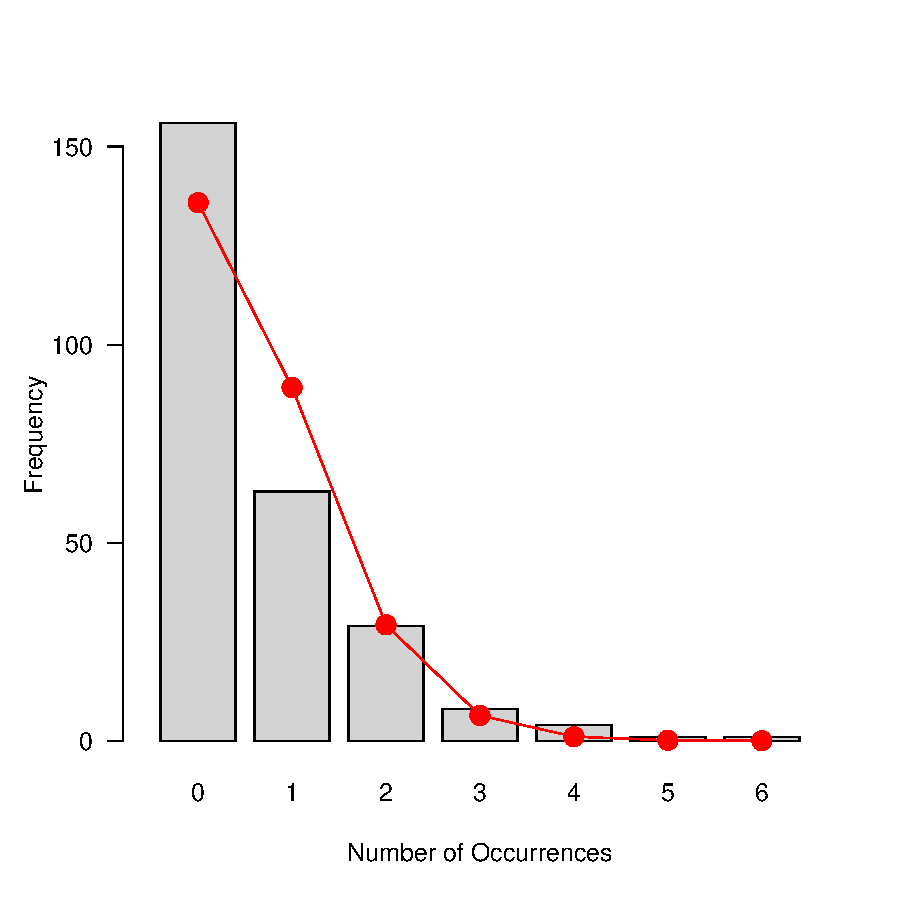
\includegraphics[width=.48\textwidth]{ch03/fig/Fed0-plots11} 
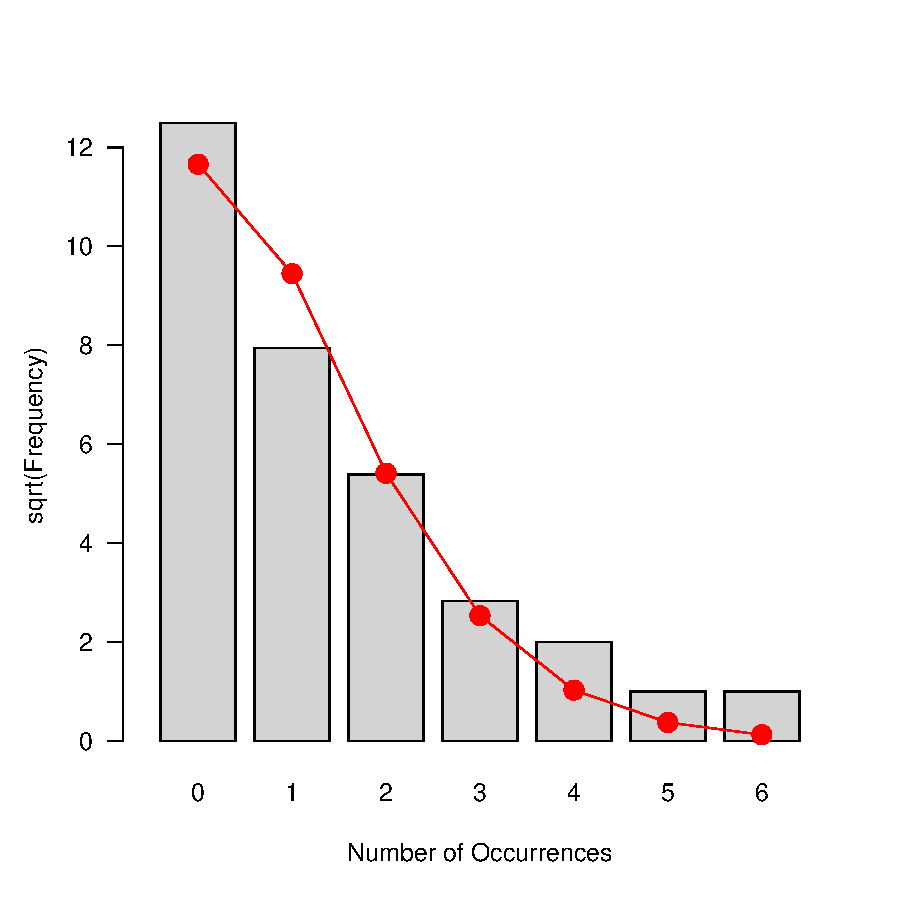
\includegraphics[width=.48\textwidth]{ch03/fig/Fed0-plots12} }

\caption[Plots for the Federalist Papers data, fitting the Poisson model]{Plots for the Federalist Papers data, fitting the Poisson model. Each panel shows the observed frequencies as bars and the fitted frequencies as a smooth curve. Left: raw frequencies; right: plotted on a square root scale to emphasize smaller frequencies.\label{fig:Fed0-plots1}}
\end{figure}


\end{knitrout}

Additional improvements over the standard plot on the scale of raw
frequencies are shown in \figref{fig:Fed0-plots2}, both of which 
use the square root scale.  The left panel 
moves the rootogram bars so their tops
are at the expected frequencies (giving a \term{hanging rootogram}).
This has the advantage that we can more easily judge the pattern
of departures against the horizontal reference line at 0, than
against the curve.

\begin{knitrout}
\definecolor{shadecolor}{rgb}{0.969, 0.969, 0.969}\color{fgcolor}\begin{kframe}
\begin{alltt}
\hlkwd{plot}\hlstd{(Fed.fit0,} \hlkwc{type}\hlstd{=}\hlstr{"hanging"}\hlstd{)}
\hlkwd{plot}\hlstd{(Fed.fit0,} \hlkwc{type}\hlstd{=}\hlstr{"deviation"}\hlstd{)}
\end{alltt}
\end{kframe}\begin{figure}[htbp]


\centerline{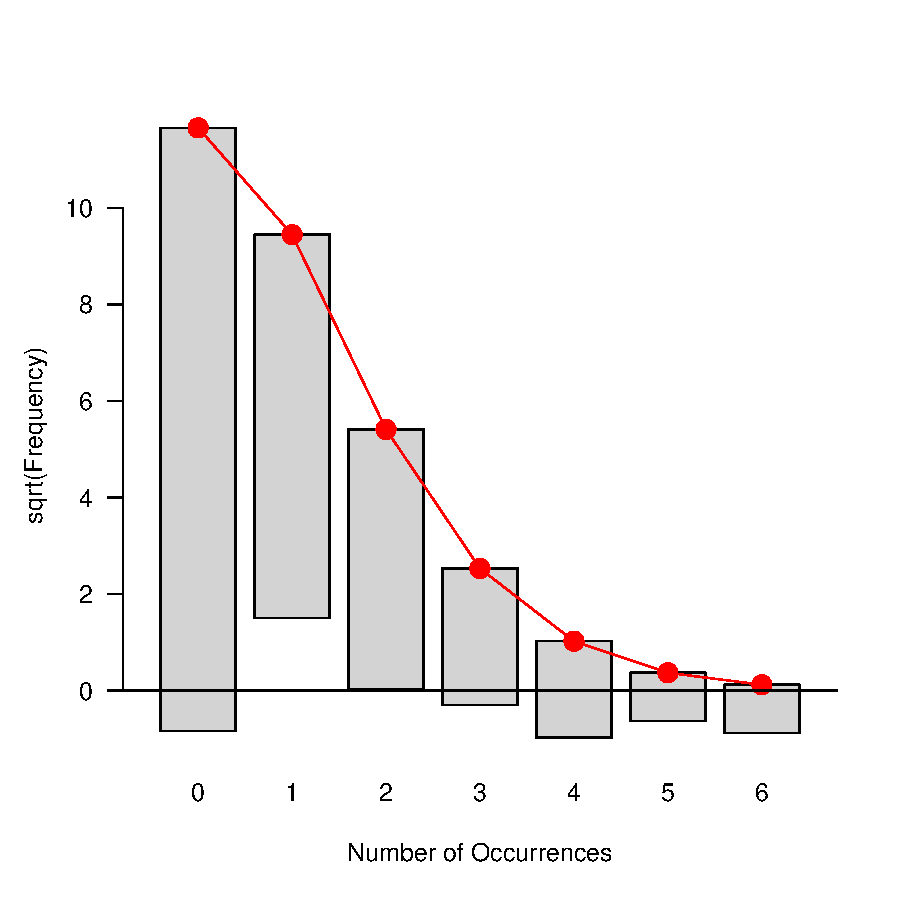
\includegraphics[width=.48\textwidth]{ch03/fig/Fed0-plots21} 
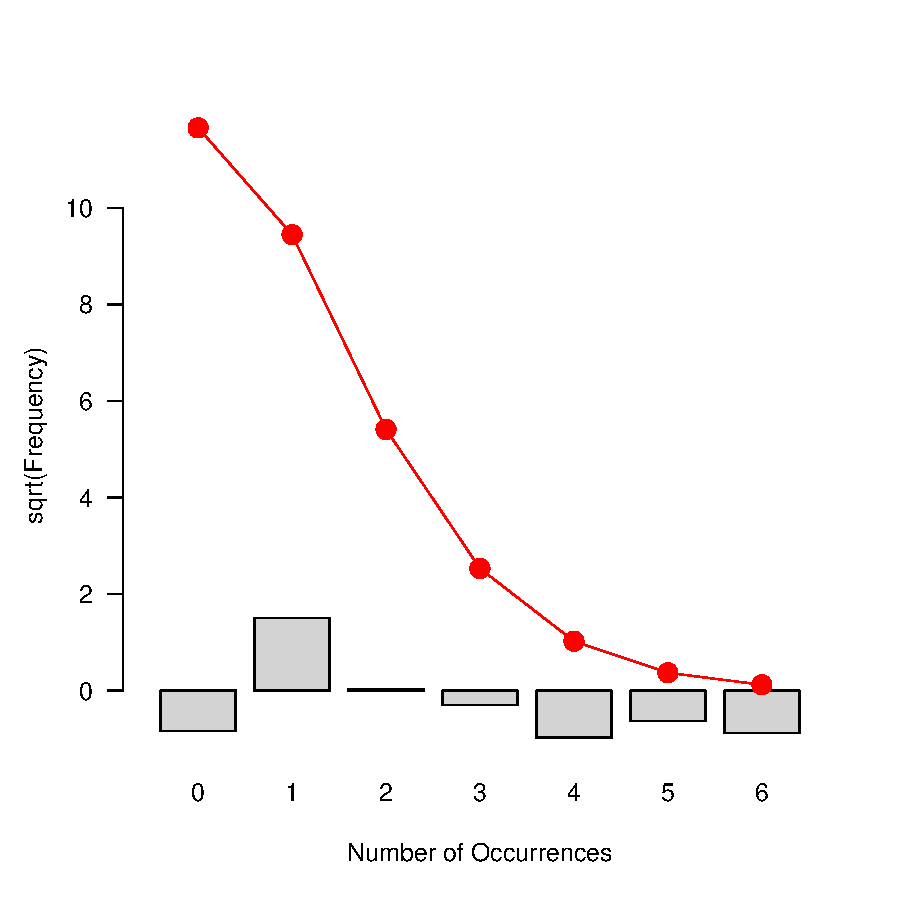
\includegraphics[width=.48\textwidth]{ch03/fig/Fed0-plots22} }

\caption[Plots for the Federalist Papers data, fitting the Poisson model]{Plots for the Federalist Papers data, fitting the Poisson model. Left: hanging rootogram; right: deviation rootogram.\label{fig:Fed0-plots2}}
\end{figure}


\end{knitrout}


A final variation is to emphasize the differences between the
observed and fitted frequencies by drawing the bars to show the
gaps between the 0 line and the (observed-expected) difference
(\figref{fig:Fed0-plots2}, right).

All of these plots are actually produced by the \func{rootogram} function
in \pkg{vcd}.  The default is \code{type="hanging"}, and there are many
options to control the plot details.

The plots in \figref{fig:Fed0-plots1} and \figref{fig:Fed0-plots2}
used the ill-fitting Poisson model on purpose to highlight how these
plots show the departure between the observed and fitted frequencies.
\figref{fig:Fed0-Fed1} compares this with the negative
binomial model, \code{Fed.fit1} which we saw has a much better, and acceptable
fit.
\begin{knitrout}
\definecolor{shadecolor}{rgb}{0.969, 0.969, 0.969}\color{fgcolor}\begin{kframe}
\begin{alltt}
\hlkwd{plot}\hlstd{(Fed.fit0,} \hlkwc{main}\hlstd{=}\hlstr{"Poisson"}\hlstd{)}
\hlkwd{plot}\hlstd{(Fed.fit1,} \hlkwc{main}\hlstd{=}\hlstr{"Negative binomial"}\hlstd{)}
\end{alltt}
\end{kframe}\begin{figure}[htbp]


\centerline{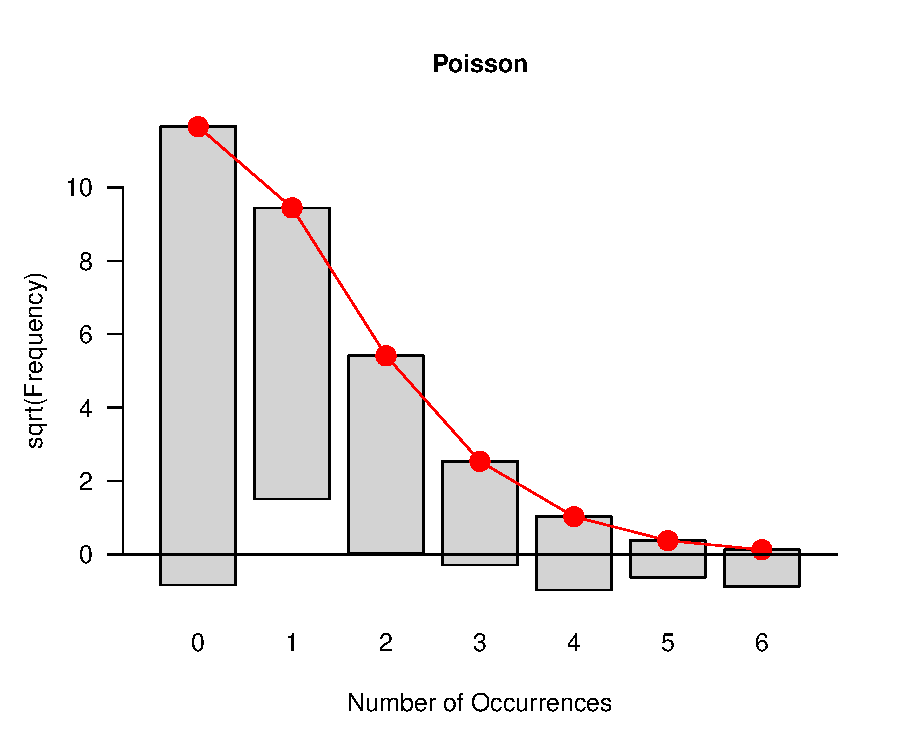
\includegraphics[width=.48\textwidth]{ch03/fig/Fed0-Fed11} 
\includegraphics[width=.48\textwidth]{ch03/fig/Fed0-Fed12} }

\caption[Hanging rootograms for the Federalist Papers data, comparing the Poisson and negative binomial models]{Hanging rootograms for the Federalist Papers data, comparing the Poisson and negative binomial models.\label{fig:Fed0-Fed1}}
\end{figure}


\end{knitrout}

Comparing the two plots in \figref{fig:Fed0-Fed1}, we can see that the Poisson model underestimates the frequencies of 0 counts and the larger counts for 4-6 occurrences.
The deviations for the negative binomial are small and unsystematic.

Finally, \figref{fig:But-fit} shows hanging rootograms for two 
atrociously bad models for the data on butterfly species in Malaya
considered in \exref{ex:butterfly}. As we will see in \secref{sec:discrete-ord},
this long-tailed distribution is better approximated by the logarithmic series
distribution, but this distribution is presently not handled by \func{goodfit}.
\begin{knitrout}
\definecolor{shadecolor}{rgb}{0.969, 0.969, 0.969}\color{fgcolor}\begin{kframe}
\begin{alltt}
\hlkwd{data}\hlstd{(Butterfly,} \hlkwc{package}\hlstd{=}\hlstr{"vcd"}\hlstd{)}
\hlstd{But.fit1} \hlkwb{<-} \hlkwd{goodfit}\hlstd{(Butterfly,} \hlkwc{type}\hlstd{=}\hlstr{"poisson"}\hlstd{)}
\hlstd{But.fit2} \hlkwb{<-} \hlkwd{goodfit}\hlstd{(Butterfly,} \hlkwc{type}\hlstd{=}\hlstr{"nbinomial"}\hlstd{)}
\hlkwd{plot}\hlstd{(But.fit1,} \hlkwc{main}\hlstd{=}\hlstr{"Poisson"}\hlstd{)}
\hlkwd{plot}\hlstd{(But.fit2,} \hlkwc{main}\hlstd{=}\hlstr{"Negative binomial"}\hlstd{)}
\end{alltt}
\end{kframe}\begin{figure}[htbp]


\centerline{\includegraphics[width=.48\textwidth]{ch03/fig/But-fit1} 
\includegraphics[width=.48\textwidth]{ch03/fig/But-fit2} }

\caption[Hanging rootograms for the Butterfly data, comparing the Poisson and negative binomial models]{Hanging rootograms for the Butterfly data, comparing the Poisson and negative binomial models. The lack of fit for both is readily apparent.\label{fig:But-fit}}
\end{figure}


\end{knitrout}


\TODO{Old sections here described the general ideas behind maximum likelihood
estimation, and methods for fitting discrete distributions as loglinear models.
What should be included in this revision?}

\section{Diagnosing discrete distributions: Ord plots}\label{sec:discrete-ord}

\ix{Ord plot|(}
Ideally, the general form chosen for a discrete distribution should
be dictated by substantive knowledge of a plausible mechanism
for generating the data.
When such knowledge is lacking, however,
we may not know which distribution is most appropriate for
some particular set of data.
In these cases, the question is often turned around, so that we seek
a distribution that fits well, and then try to understand the mechanism
in terms of aspects of the underlying probability theory (independent trials,
rare events, waiting-time to an occurrence, and so forth).

Although it is possible to fit each of several possibilities,
the summary goodness-of-fit statistics can easily be influenced by
one or two disparate cells, or additional (ignored or unknown) factors.
One simple alternative is a plot suggested by
\citet{Ord:67} which may be used to diagnose
the form of the discrete distribution.  

Ord showed that a linear
relationship of the form,
\begin{equation} \label{eq:ord}
  \frac{ k \,  p(k) } { p(k-1) }
\equiv \frac{ k \,  n_k } { n_{k-1} }
 = a  +  b \,  k \comma
\end{equation}
holds for each of the Poisson, binomial, negative binomial, and
logarithmic series distributions, and these distributions are
distinguished by the signs of the intercept,
$a$, and slope, $b$, as shown in
\tabref{tab:ordparm}.
\begin{table}[htb]
\caption[Diagnostic slope and intercept for four discrete distributions]{Diagnostic slope and
intercept for four discrete distributions.  The ratios $k n_k / n_{k-1}$ plotted
against $k$ should appear as a straight line, whose slope and intercept
determine the particular distribution.}
\label{tab:ordparm}
\begin{center}
%\vspace{1ex}
\begin{tabular}{|ccll|}\hline
Slope & Intercept & Distribution & Parameter \\
(b)   & (a)       & (parameter)  &  estimate \\ \hline
0     &  $+$      &  Poisson (\(\lambda\)) & \(\lambda = a\)    \\
$-$   &  $+$      &  Binomial (n, p)       & \(p = b / (b-1)\)  \\
$+$   &  $+$      &  Negative binomial (n,p)      & \(p = 1 - b\)      \\
$+$   &  $-$      &  Log.\ series (\(\theta\)) & \(\theta =  b\) \\
      &      &                     &   \(\theta = - a\) \\ \hline
\end{tabular}
\end{center}
\end{table}



The slope, \(b\),
in \eqref{eq:ord} is zero for the
Poisson, negative for the binomial, and positive for the negative
binomial and logarithmic series distributions; the latter two are
distinguished by their intercepts. In practical applications of this
idea, the details are important:  how to fit the line, and how to determine
if the pattern of signs are sufficient to reasonably provide a
diagnosis of the distribution type.

One difficulty in applying this technique is that the number of points
(distinct values of $k$)
in the Ord plot is often small, and the sampling variances of
\(k \,  n_k /  n_{k-1}\) can vary enormously.
A little reflection indicates that points where $n_k$ is small
should be given less weight in determining the slope of the
line (and hence determining the form of the distribution).
In applications it has been found that
using a weighted least squares fit of \(k \,
n_k /  n_{k-1}\) on \(k\), using weights of \(w_k = \sqrt { n_k -1
}\)
produces reasonably good
automatic diagnosis of the form of a
probability distribution. Moreover, to judge whether a coefficient is
positive or negative, a small tolerance is used;  if none of the distributions
can be classified, no parameters are estimated.  Caution is advised in
accepting the conclusion, because it is based on these simple heuristics.

In the \Rpackage{vcd} this method is implemented in the \func{Ord\_plot}
function. The essential ideas are illustrated using the 
\data{Butterfly} data below, which produces \figref{fig:ordplot1}. Note that the
function returns (invisibly) the values of the intercept and slope in the
weighted LS regression.

\begin{knitrout}
\definecolor{shadecolor}{rgb}{0.969, 0.969, 0.969}\color{fgcolor}\begin{kframe}
\begin{alltt}
\hlstd{ord} \hlkwb{<-} \hlkwd{Ord_plot}\hlstd{(Butterfly,}
                \hlkwc{main} \hlstd{=} \hlstr{"Butterfly species collected in Malaya"}\hlstd{,}
                \hlkwc{gp}\hlstd{=}\hlkwd{gpar}\hlstd{(}\hlkwc{cex}\hlstd{=}\hlnum{1}\hlstd{),} \hlkwc{pch}\hlstd{=}\hlnum{16}\hlstd{)}
\hlstd{ord}
\end{alltt}
\begin{verbatim}
## Intercept     Slope 
##    -0.709     1.061
\end{verbatim}
\end{kframe}\begin{figure}[htbp]


\centerline{\includegraphics[width=.5\textwidth]{ch03/fig/ordplot1} }

\caption[Ord plot for the Butterfly data]{Ord plot for the Butterfly data. The slope and intercept in the plot correctly diagnoses the log-series distribution.\label{fig:ordplot1}}
\end{figure}


\end{knitrout}

In this plot, the black line shows the usual OLS regression fit of
frequency, $n_k$ on number of occurrences, $k$;  the red line shows
the weighted least squares fit, using weights of $\sqrt{n_k-1}$.
In this case, the two lines are fairly close together, as regards
their intercepts and slopes.  The positive slope and negative intercept
diagnoses this as a log-series distribution.
\ix{logarithmic series distribution}

In other cases, the number of distinct points (values of $k$) is small,
and the sampling variances of the ratios $ k \, n_k / n_{k-1}$ can vary 
enormously.  The following examples illustrate some other distributions
and some of the details of the heuristics.

\DONE{In \code{vcd\_1.3-2}, fixed \func{Ord\_plot} to provide control of \code{lwd}, \code{lty}, etc.}

\subsubsection{Ord plot examples}
\begin{Example}[horskick3]{Death by horse kick}
The results below show the calculations for
the horse kicks data, with the frequency ratio \({ k \,  n_k } /  { n_{k-1}
}\) labeled \texttt{y}.  

\begin{knitrout}
\definecolor{shadecolor}{rgb}{0.969, 0.969, 0.969}\color{fgcolor}\begin{kframe}
\begin{alltt}
\hlkwd{data}\hlstd{(HorseKicks,} \hlkwc{package}\hlstd{=}\hlstr{"vcd"}\hlstd{)}
\hlstd{nk} \hlkwb{<-} \hlkwd{as.vector}\hlstd{(HorseKicks)}
\hlstd{k} \hlkwb{<-} \hlkwd{as.numeric}\hlstd{(}\hlkwd{names}\hlstd{(HorseKicks))}
\hlstd{nk1} \hlkwb{<-} \hlkwd{c}\hlstd{(}\hlnum{NA}\hlstd{, nk[}\hlopt{-}\hlkwd{length}\hlstd{(nk)])}
\hlstd{y} \hlkwb{<-} \hlstd{k} \hlopt{*} \hlstd{nk}\hlopt{/}\hlstd{nk1}
\hlstd{weight} \hlkwb{=} \hlkwd{sqrt}\hlstd{(}\hlkwd{pmax}\hlstd{(nk,} \hlnum{1}\hlstd{)} \hlopt{-} \hlnum{1}\hlstd{)}
\hlstd{(ord.df} \hlkwb{<-} \hlkwd{data.frame}\hlstd{(k, nk, nk1, y, weight))}
\end{alltt}
\begin{verbatim}
##   k  nk nk1      y weight
## 1 0 109  NA     NA 10.392
## 2 1  65 109 0.5963  8.000
## 3 2  22  65 0.6769  4.583
## 4 3   3  22 0.4091  1.414
## 5 4   1   3 1.3333  0.000
\end{verbatim}
\begin{alltt}
\hlkwd{coef}\hlstd{(}\hlkwd{lm}\hlstd{(y} \hlopt{~} \hlstd{k,} \hlkwc{weights}\hlstd{=weight,} \hlkwc{data}\hlstd{=ord.df))}
\end{alltt}
\begin{verbatim}
## (Intercept)           k 
##     0.65602    -0.03414
\end{verbatim}
\end{kframe}
\end{knitrout}


The weighted least squares line, with weights
\(w_k\), has a slope (-0.03) close to zero, indicating the Poisson
distribution.%
\footnote{
The heuristic adopted in \func{Ord\_plot} uses a tolerance of 0.1
to decide if a coefficient is negative, zero, or positive.
}
The estimate \(\lambda = a = .656\) compares
favorably with the MLE, $\lambda=0.610$ and the
value from the Poissonness plot, shown in the
following section.  The call to \func{Ord\_plot} below
produces \figref{fig:ordplot2}.
\ixd{death by horse kick}
\ix{Poisson distribution}

\begin{knitrout}
\definecolor{shadecolor}{rgb}{0.969, 0.969, 0.969}\color{fgcolor}\begin{kframe}
\begin{alltt}
\hlkwd{Ord_plot}\hlstd{(HorseKicks,}
         \hlkwc{main} \hlstd{=} \hlstr{"Death by horse kicks"}\hlstd{,} \hlkwc{gp}\hlstd{=}\hlkwd{gpar}\hlstd{(}\hlkwc{cex}\hlstd{=}\hlnum{1}\hlstd{),} \hlkwc{pch}\hlstd{=}\hlnum{16}\hlstd{)}
\end{alltt}
\end{kframe}\begin{figure}[htbp]


\centerline{\includegraphics[width=.5\textwidth]{ch03/fig/ordplot2} }

\caption[Ord plot for the HorseKicks data]{Ord plot for the HorseKicks data. The plot correctly diagnoses the Poisson distribution.\label{fig:ordplot2}}
\end{figure}


\end{knitrout}

\end{Example}

\begin{Example}[madison3]{Federalist papers}
\figref{fig:ordplot3} (left) shows the Ord plot for the \data{Federalist} data.
The slope is positive, so either the
negative binomial or log series are possible, according to \tabref{tab:ordparm}.
The intercept is
essentially zero, which is ambiguous.  However, the logarithmic
series requires \(b \approx  - a\), so the negative binomial is a
better choice.  \citet{MostellerWallace:63,MostellerWallace:84} did in fact find a reasonably
good fit to this distribution. Note that there is one apparent outlier,
at $k=6$, whose effect on the OLS line is to increase the slope and decrease
the intercept.
\ix{logarithmic series distribution}
\ix{negative binomial distribution}
\ixd{Federalist papers}
\end{Example}

\begin{knitrout}
\definecolor{shadecolor}{rgb}{0.969, 0.969, 0.969}\color{fgcolor}\begin{kframe}
\begin{alltt}
\hlkwd{Ord_plot}\hlstd{(Federalist,} \hlkwc{main} \hlstd{=} \hlstr{"Instances of 'may' in Federalist papers"}\hlstd{,}
         \hlkwc{gp}\hlstd{=}\hlkwd{gpar}\hlstd{(}\hlkwc{cex}\hlstd{=}\hlnum{1}\hlstd{),} \hlkwc{pch}\hlstd{=}\hlnum{16}\hlstd{)}
\hlkwd{Ord_plot}\hlstd{(WomenQueue,} \hlkwc{main} \hlstd{=} \hlstr{"Women in queues of length 10"}\hlstd{,}
         \hlkwc{gp}\hlstd{=}\hlkwd{gpar}\hlstd{(}\hlkwc{cex}\hlstd{=}\hlnum{1}\hlstd{),} \hlkwc{pch}\hlstd{=}\hlnum{16}\hlstd{)}
\end{alltt}
\end{kframe}\begin{figure}[htbp]


\centerline{\includegraphics[width=.48\textwidth]{ch03/fig/ordplot31} 
\includegraphics[width=.48\textwidth]{ch03/fig/ordplot32} }

\caption[Ord plots for the Federalist (left) and WomenQueue (right) data sets]{Ord plots for the Federalist (left) and WomenQueue (right) data sets.\label{fig:ordplot3}}
\end{figure}


\end{knitrout}


\begin{Example}[queues]{Women in queues}
\citet{JinkinsonSlater:81,HoaglinTukey:85}
give the frequency distribution of the number of females observed in 100
queues of length 10 in a London Underground station, recorded
in the data set \data{WomenQueue} in \pkg{vcd}.
\begin{knitrout}
\definecolor{shadecolor}{rgb}{0.969, 0.969, 0.969}\color{fgcolor}\begin{kframe}
\begin{alltt}
\hlkwd{data}\hlstd{(WomenQueue,} \hlkwc{package}\hlstd{=}\hlstr{"vcd"}\hlstd{)}
\hlstd{WomenQueue}
\end{alltt}
\begin{verbatim}
## nWomen
##  0  1  2  3  4  5  6  7  8  9 10 
##  1  3  4 23 25 19 18  5  1  1  0
\end{verbatim}
\end{kframe}
\end{knitrout}


If it is assumed that people line up independently, and that
men and women are equally likely to be found in a queue
(not necessarily reasonable assumptions),
then the number of women out of 10
would have a (symmetric) binomial distribution with parameters $n=10$ and
$p=\frac12$.
However, there is no real reason to expect that males and females are
equally likely to be found in queues in the London underground,
so we may be interested in estimating $p$ from the data
and determining if a binomial distribution fits.
\ix{binomial distribution}

\figref{fig:ordplot3} (right) shows the Ord plot for these data.
The negative slope and positive intercept clearly diagnose this distribution
as binomial.  The rough estimate of $\hat{p} = b/(1-b) = 0.53$ indicates that
women are slightly more prevalent than men in these data for the London 
underground. 
\end{Example}

\subsubsection{Limitations of Ord plots}
Using a single simple diagnostic plot to determine one of four common discrete
distributions is advantageous, but your enthusiasm should be
dampened by several weaknesses:

\begin{itemize*}
\item The Ord plot lacks resistance, since a single discrepant
       frequency affects the points $n_k / n_{k-1}$
       for both \(k\) and \(k  +  1\).

\item The sampling variance of \(k \,  n_k /  n_{k-1}\) fluctuates
       widely
       \citep{HoaglinTukey:85,JinkinsonSlater:81}.  
       The use of weights \(w_k\) helps, but is purely a
       heuristic device. The \func{Ord\_plot} function explicitly shows both
       the OLS line and the WLS line, which provides some indication of the
       effect of the points on the estimation of slope and intercept.
\end{itemize*}


\ix{Ord plot|)}


\section{Poissonness plots and generalized distribution plots}\label{sec:discrete-Poissonness}

\ix{Poissonness plot|(}

The \term{Poissonness plot}
\citep{Hoaglin:80}
is a robust plot to sensitively determine how well a 
one-way table of frequencies follows a \IX{Poisson distribution}.
It plots a quantity called a count metameter
against \(k\), designed
so that the result will be points along a
straight line when the data follow a \IX{Poisson distribution}.  When the
data deviate from a Poisson, the points will be curved.
\citet{HoaglinTukey:85}
develop similar plots for other discrete distributions,
including the binomial, negative binomial, and logarithmic series
distributions.  We first describe the features and construction
of these plots for the Poisson distribution and then (\secref{sec:})
the extension to other distributions.


\ix{binomial distribution}
\ix{negative binomial distribution}

\subsection{Features of the Poissonness plot}
The Poissonness plot has the following desirable features:
\begin{itemize}
\item \boldital{Resistance}: a single discrepant value of \(n_k\)
       affects only the point at value \(k\).  (In the Ord plot
       it affects each of its neighbors.)
\item \boldital{Comparison standard}:  An approximate confidence
       interval can be found for each point, indicating its inherent
       variability and helping to judge whether each point is
       discrepant.
\item \boldital{Influence}:  Extensions of the method result in
       plots which show the effect of each point on the estimate of
       the main parameter of the distribution (\(\lambda\) in the
       Poisson).
\end{itemize}

\subsection{Plot construction}
Assume, for some fixed \(\lambda\), each observed frequency, \(n_k\)
equals the expected frequency, \(m_k = N p_k\).  Then, setting
\(n_k = N p_k  = N { e^{ - \lambda } \:  \lambda^k } /  { k ! }\),
and taking logs of both sides gives
\begin{equation*}
  \log ( n_k ) = \log \,  N - \lambda  +  k \,  \log \,  \lambda  -
  \log \,  k !
  \period
\end{equation*}
This can be rearranged to a linear equation in $k$,
\begin{equation} \label{eq:poispl}
  \phi \,  ( n_k ) \equiv \log \left(  \frac{ k ! \:  n_k } {N} \right)
 = - \lambda  +  ( \log \,  \lambda ) \,  k
 \period
\end{equation}
The left side of \eqref{eq:poispl} is called the \term{count metameter}, and
denoted \(\phi \,  ( n_k )\).  Hence,
plotting \(\phi ( n_k )\) against \(k\) should give a straight line of the form
\(\phi ( n_k )= a + b k\) with
\begin{itemize*}
\item slope = \(\log  \,  \lambda\)
\item intercept = \(- \lambda\)
\end{itemize*}
when the observed frequencies follow a Poisson distribution.
If the points in this plot are close enough to a straight line,
then an estimate of $\lambda$ may be obtained from the slope $b$ of the line,
$\hat{\lambda} = e^b$ should be reasonably close in value
to the MLE of $\lambda$, $\hat{\lambda} = \bar{x}$.
In this case, we might as well use the MLE as our estimate.

\subsubsection{Leveled plot}
If we have a preliminary estimate $\lambda_0$ of $\lambda$,
we can use this to give a new plot where the reference line
is horizontal, making comparison of the points with the line
easier.
In this leveled plot the vertical coordinate $\phi (n_k)$ is modified to
\begin{equation}\label{eq:pois-leveled}
 \phi ' (n_k) = \phi (n_k) + \lambda_0 - k \log \lambda_0
 \period
\end{equation}
When the data follow a Poisson distribution with parameter
$\lambda$, the modified plot will have
\begin{itemize*}
\item slope = \(\log  \lambda - \log  \lambda_0 = \log ( \lambda / \lambda_0 ) \)
\item intercept = \(\lambda_0 - \lambda\)
\end{itemize*}
In the ideal case, where our estimate of $\lambda_0$ is close to the true
$\lambda$, the line will be approximately
horizontal at $\phi(n_k) ' = 0$.
The modified plot is particularly useful in conjunction with the
confidence intervals for individual points described below.

\subsubsection{Confidence intervals}
The goal of the Poissonness plot is to determine whether the points
are ``sufficiently linear'' to conclude that the Poisson distribution
is adequate for the data. Confidence intervals for the points can help
you decide, and also show the relative precision of the points in these
plots.

For example, when one or two points deviate from an otherwise nearly linear
relation,
it is helpful to determine whether the discrepancy is consistent with
chance variation.
As well, we must recognize that classes with small frequencies $n_k$
are less precise than classes with large frequencies.

\citet{HoaglinTukey:85} develop approximate confidence intervals
for $\log (m_k)$ for each point in the Poissonness plot.
These are calculated as
\begin{equation}\label{eq:poisCI}
\phi \left( n_k^{*}\right) \pm h_k
\end{equation}
where the count metameter function is calculated using a modified frequency $%
n_k^{*}$, defined as
\begin{equation*}
n_k^{*}= \left\{
\begin{array}{ll}
n_k-.8n_k-.67 & n\geq 2 \\
1/e & n=1 \\
\textrm{undefined} & n=0
\end{array}
\right.
\end{equation*}
%
and $h_k$ is the half-width of the 95\% confidence interval,
\begin{equation*}
h_k=1.96\frac{\sqrt{1-\widehat{p}_k}}{[n_k-(.25\widehat{p}_k+.47)\sqrt{n_k}%
]^{1/2}}
\end{equation*}
and $\hat{p}_k = n_k / N$.


\subsection[The distplot function]{The \func{distplot} function}
Poissonness plots (and versions for other distributions)
are produced by the function \func{distplot} in \pkg{vcd}.
As with \func{Ord\_plot}, the first argument is
either a vector of counts, a one-way table of frequencies of counts or a data frame or matrix with frequencies in the first column and the corresponding counts in the second column. Nearly all of the examples in this chapter use one-way tables of counts.

The \code{type} argument specifies the type of distribution. For \code{type = "poisson"},
specifying a value for \code{lambda} $=\lambda_0$ gives the leveled version of the
plot.

\begin{Example}[horsekick3]{Death by horse kick}
The calculations for the Poissonness plot, including confidence
intervals, are shown below for the \data{HorseKicks} data.  The 
call to \func{distplot}
produces the plot in the left panel of
\figref{fig:distplot1}.  

\begin{knitrout}
\definecolor{shadecolor}{rgb}{0.969, 0.969, 0.969}\color{fgcolor}\begin{kframe}
\begin{alltt}
\hlkwd{data}\hlstd{(}\hlstr{"HorseKicks"}\hlstd{,} \hlkwc{package}\hlstd{=}\hlstr{"vcd"}\hlstd{)}
\hlstd{dp} \hlkwb{<-} \hlkwd{distplot}\hlstd{(HorseKicks,} \hlkwc{type} \hlstd{=} \hlstr{"poisson"}\hlstd{,}
  \hlkwc{xlab}\hlstd{=}\hlstr{"Number of deaths"}\hlstd{,} \hlkwc{main}\hlstd{=}\hlstr{"Poissonness plot: HorseKicks data"}\hlstd{)}
\hlkwd{print}\hlstd{(dp,} \hlkwc{digits}\hlstd{=}\hlnum{4}\hlstd{)}
\end{alltt}
\begin{verbatim}
##   Counts Freq Metameter CI.center CI.width CI.lower CI.upper
## 1      0  109    -0.607   -0.6131   0.1305  -0.7436  -0.4827
## 2      1   65    -1.124   -1.1343   0.2069  -1.3412  -0.9274
## 3      2   22    -1.514   -1.5451   0.4169  -1.9620  -1.1281
## 4      3    3    -2.408   -2.6607   1.3176  -3.9783  -1.3431
## 5      4    1    -2.120   -3.1203   2.6887  -5.8089  -0.4316
\end{verbatim}
\end{kframe}
\end{knitrout}

In this plot, the open circles show the calculated
observed values of the count \code{Metameter} = $\phi \,  ( n_k )$.
The smaller filled points show the centers of the confidence intervals,
\code{CI.center} = $\phi \left( n_k^{*}\right)$ (\eqref{eq:poisCI}),
and the dashed lines show the extent of the confidence intervals.

The fitted least squares line has a slope of -0.431, which would
indicate $\lambda = e^{-0.431} = 0.65$.  This compares well with the MLE,
$\lambda = \bar{x} = 0.61$.
\ixd{death by horse kick}

Using \code{lambda = 0.61} as below gives the leveled version shown in 
the right panel of \figref{fig:distplot1}.
\begin{knitrout}
\definecolor{shadecolor}{rgb}{0.969, 0.969, 0.969}\color{fgcolor}\begin{kframe}
\begin{alltt}
\hlcom{# leveled version, specifying lambda}
\hlkwd{distplot}\hlstd{(HorseKicks,} \hlkwc{type} \hlstd{=} \hlstr{"poisson"}\hlstd{,} \hlkwc{lambda} \hlstd{=} \hlnum{0.61}\hlstd{,}
  \hlkwc{xlab}\hlstd{=}\hlstr{"Number of deaths"}\hlstd{,} \hlkwc{main}\hlstd{=}\hlstr{"Leveled Poissonness plot"}\hlstd{)}
\end{alltt}
\end{kframe}
\end{knitrout}


\begin{figure}[htbp]
\centerline{
\includegraphics[width=.48\textwidth]{ch03/fig/distplot1} 
\includegraphics[width=.48\textwidth]{ch03/fig/distplot2}
}
\caption[Poissonness plots for the HorseKick data]{Poissonness plots for the HorseKick data. Left: standard plot; right: leveled plot.\label{fig:distplot1}}
\end{figure}
In both plots the fitted line is within the confidence intervals,
indicating the adequacy of the Poisson model for these data.
The widths of the intervals for $k > 2$ are graphic reminders that these observations
have decreasingly low precision where the counts $n_k$ are small.

\end{Example}

\subsection{Leverage and influence}
\TODO{This subsection should be omitted, unless we extend the calculation and plotting 
methods.}

\ix{Poissonness plot|)}

\subsection{Plots for other distributions}\label{sec:discrete-other}
As described in \secref{sec:pwrseries}, the binomial, Poisson, negative binomial,
geometric, and logseries distributions are all members of the
general  power series family of discrete distributions.
For this family, \citet{HoaglinTukey:85} develop similar plots
of a count metameter against $k$ which appear as a straight line
when a data distribution follows a given family member.

The distributions which can be analyzed in this way are shown in
\tabref{tab:distparms}, with the interpretation given to the
slope and intercept in each case.
For example, for the Binomial distribution, a ``binomialness''
plot is constructed by plotting $\log n_k^{*} / N \binom{n}{k}$
against $k$.  If the points in this plot approximate a straight
line, the slope is interpreted as $\log (p/(1-p))$, so the
binomial parameter $p$ may be estimated as $p = e^b/(1+e^b)$.
\begin{table}[htb]
\caption[Plot parameters for five discrete distributions]{Plot parameters for five discrete distributions. In each case the count metameter, $\phi
(n_k^{*})$ is plotted against $k$, yielding a straight line when the data
follow the given distribution.}
\label{tab:distparms}
 \begin{center}
\begin{tabular}{p{2.4cm}llll}
  \hline\\[.5ex]
  \tableheader
%              & Probability      & Count                      & Theoretical & Theoretical \\
%Distributiion & function, $p(k)$ & metameter, $\phi(n_k^{*})$ & Slope ($b$) & Intercept ($a$)\\[1ex]
  \multilineL{Distribution\\} & \multilineL{Probability\\function, $p(k)$} & \multilineL{Count)\\metameter, $\phi(n_k^{*})$} & \multilineL{Theoretical\\ slope ($b$)} &
  \multilineL{Theoretical\\ intercept ($a$)}
  \hline \\[.5ex]
Poisson          & $e^{-\lambda }\lambda ^k/k!$ & $\log (k!n_k^{*}/N)$ & $\log
(\lambda )$ & -$\lambda $ \\[.7ex]
%
Binomial          & $\binom nkp^k(1-p)^{n-k}$ & $\log \left( n_k^{*}/N\binom
nk\right) $ & $\log \left(\frac{p}{1-p}\right)$ & $n\log (1-p)$ \\[.7ex]
%
Negative binomial & $\binom{n+k-1}kp^n(1-p)^k$ & $\log \left( n_k^{*}/N%
\binom{n+k-1}k\right) $ & $\log (1-p)$ & $n\log (p)$ \\[.7ex]
%
Geometric         & $p(1-p)^k$ & $\log \left( n_k^{*}/N\right) $ & $\log (1-p)$ & $\log (p)$ \\[.7ex]
%
Log series        & $\theta ^k/[-k\log (1-\theta )]$ & $\log \left(
kn_k^{*}/N\right) $ & $\log (\theta )$ & $-\log \left( -\log (1-\theta)\right) $ \\[1ex]%
  \hline
  \multicolumn{5}{p{\textwidth}}{\emph{Source}: adapted from \citet{HoaglinTukey:85}, Table 9-15.} \\
\end{tabular}
 \end{center}
\end{table}



Unlike the Ord plot, a different plot is required for each distribution,
because the count metameter, \(\phi ( n_k )\), differs
from distribution to distribution.
Moreover, systematic deviation from a linear relationship does not
       indicate which distribution provides a better fit.
However, the attention to robustness, and the availability of confidence
intervals and influence diagnostics make this a highly useful tool
for visualizing discrete distributions.

\begin{Example}[saxony-distplot]{Families in Saxony}
Our analysis in \exref{ex:saxony1} and \exref{ex:saxfit} of
the Saxony data
showed that the distribution of male children had slightly heavier tails
than the binomial, meaning the observed distribution is overdispersed.
We can see this in the \func{goodfit} plot shown in \figref{fig:distplot3} (left),
and even more clearly in the distribution diagnostic
plot produced
by \func{distplot} in the right panel of \figref{fig:distplot3}.
For a binomial distribution, we call
this distribution plot a ``binomialness plot''.

\begin{knitrout}
\definecolor{shadecolor}{rgb}{0.969, 0.969, 0.969}\color{fgcolor}\begin{kframe}
\begin{alltt}
\hlkwd{data}\hlstd{(}\hlstr{"Saxony"}\hlstd{,} \hlkwc{package}\hlstd{=}\hlstr{"vcd"}\hlstd{)}
\hlkwd{plot}\hlstd{(}\hlkwd{goodfit}\hlstd{(Saxony,} \hlkwc{type}\hlstd{=}\hlstr{"binomial"}\hlstd{,} \hlkwc{par}\hlstd{=}\hlkwd{list}\hlstd{(}\hlkwc{size}\hlstd{=}\hlnum{12}\hlstd{)))}
\hlkwd{distplot}\hlstd{(Saxony,} \hlkwc{type} \hlstd{=} \hlstr{"binomial"}\hlstd{,} \hlkwc{size} \hlstd{=} \hlnum{12}\hlstd{,}
  \hlkwc{xlab}\hlstd{=}\hlstr{"Number of males"}\hlstd{)}
\end{alltt}
\end{kframe}\begin{figure}[htbp]


\centerline{\includegraphics[width=.49\textwidth]{ch03/fig/distplot31} 
\includegraphics[width=.49\textwidth]{ch03/fig/distplot32} }

\caption[Diagnostic plots for males in Saxony families]{Diagnostic plots for males in Saxony families. Left: \func{goodfit} plot; right: \func{distplot} plot. Both plots show heavier tails than in a binomial distribution.\label{fig:distplot3}}
\end{figure}


\end{knitrout}

The weight of evidence is thus that, as simple as the binomial might be,
it is inadequate to fully explain the distribution of sex ratios in this
large sample of families of 12 children.
To understand this data better, it is necessary to question the assumptions
of the binomial (births of males are independent
Bernoulli trials with constant probability $p$)
as a model for this birth distribution and/or find a more
adequate model.%
\footnote{
On these questions, \citet{Edwards:1958} reviews
numerous other studies of these Geissler's data, and fits a so-called
\term{$\beta$-binomial} model proposed by \citet{Skellam:1948},
where $p$ varies among families according to a $\beta$ distribution.
He concludes that there
is evidence that $p$ varies between families of the same size.  One suggested
explanation is that family decisions to have a further child is influenced by
the balance of boys and girls among their earlier children.
}
\end{Example}


\begin{Example}[federalist-distplot]{Federalist papers}
In \exref{ex:Fedfit} we carried out GOF tests for the Poisson and
negative binomial models with the Federalist papers data;
\figref{fig:Fed0-Fed1} showed the corresponding rootogram plots.
\figref{fig:distplot5} compares these two using the diagnostic plots of
this section. Again the Poisson shows systematic departure from the 
linear relation required in the Poissonness plot, while the
negative binomial model provides an acceptable fit to
these data.
\begin{knitrout}
\definecolor{shadecolor}{rgb}{0.969, 0.969, 0.969}\color{fgcolor}\begin{kframe}
\begin{alltt}
\hlkwd{distplot}\hlstd{(Federalist,} \hlkwc{type} \hlstd{=} \hlstr{"poisson"}\hlstd{,} \hlkwc{xlab}\hlstd{=}\hlstr{"Occurrences of 'may'"}\hlstd{)}
\hlkwd{distplot}\hlstd{(Federalist,} \hlkwc{type} \hlstd{=} \hlstr{"nbinomial"}\hlstd{,} \hlkwc{xlab}\hlstd{=}\hlstr{"Occurrences of 'may'"}\hlstd{)}
\end{alltt}
\end{kframe}\begin{figure}[htbp]


\centerline{\includegraphics[width=.49\textwidth]{ch03/fig/distplot51} 
\includegraphics[width=.49\textwidth]{ch03/fig/distplot52} }

\caption[Diagnostic plots for the Federalist papers data]{Diagnostic plots for the Federalist papers data. Left: Poissonness plot; right: negative binomialness plot.\label{fig:distplot5}}
\end{figure}


\end{knitrout}

\end{Example}

\section{Fitting discrete distributions as generalized linear models}\label{sec:fitglm}

In \secref{sec:pwrseries}, we described how the common discrete distributions
are all members of the general power series family.  This provides the
basis for the generalized distribution plots described in \secref{sec:discrete-other}.
Another general family of distributions---the \term{exponential family}---%
includes most of the common continuous distributions:
the normal, gamma, exponential, and others,
and is the basis of the class of generalized linear models fit
by \func{glm}.

A clever approach by
\citet{LindseyMersch:92}, \citet[\S 6.1]{Lindsey:95} shows how various discrete
(and continuous)
distributions can be fit to frequency data using generalized linear models
for log frequency (which are equivalent to Poisson \loglin models).
The uniform, geometric, binomial, and the
Poisson distributions may all be fit easily in this way, but the idea extends
to some other distributions, such as the \term{double binomial} distribution,
that allows a separate parameter for overdispersion relative to the binomial.
A clear advantage is that this method gives estimated standard errors for the
distribution parameters as well as estimated confidence intervals
for fitted probabilities.

The essential idea is that, for frequency data, any distribution in the
exponential family may be represented by a linear model for the logarithm
of the cell frequency, with a Poisson distribution for errors,
otherwise known as a ``Poisson \loglin\ regression model''.
These have the form
\begin{equation*}
\log (N \pi_k) = \textrm{ offset } + \beta_0 + \vec{\beta}\trans \vec{S}(k)
 \comma
\end{equation*}
where $N$ is the total frequency, $\pi_k$ is the modeled probability
of count $k$, 
$\vec{S}(k)$ is a vector of zero or more sufficient statistics for the
canonical parameters of the exponential family distribution,
and the offset term is a value which does not depend on the
parameters.  

\tabref{tab:expfamily} shows the sufficient statistics and
offsets for several discrete distributions.
See \citet{LindseyMersch:92} for further details, and definitions
for the double-binomial distribution,%
\footnote{
In \R, the double binomial distribution is implemented in the 
\Rpackage{rmutil}, providing the standard complement of
density function (\func{ddoublebinom}), CDF (\func{pdoublebinom}),
quantiles (\func{qdoublebinom})
and random generation (\func{rdoublebinom}).
}
and \citet[pp. 130--133]{Lindsey:95}
for his analysis of the \data{Saxony} data using this distribution.
\citet{LindseyAltham:1998} provide an analysis of the 
complete Geissler data using several different models to
handle overdispersion.
\begin{table}[tb]
 \caption{Poisson \loglin\ representations for some discrete distributions}\label{tab:expfamily}
 \begin{center}
{\renewcommand{\arraystretch}{1.2}
 \begin{tabular}{lll}
  \hline
  \tableheader
  Distribution & Sufficient statistics & Offset \\
  \hline
  Geometric & $k$ \\
  Poisson & $k$ & $-\log(k!)$ \\
  Binomial & $k$ & $\log{\binom{n}{k}}$ \\
  Double binomial & $k, k \log(k) + (n-k) \log(n-k)$ & $\log{\binom{n}{k}}$ \\
  \hline
 \end{tabular}
}
 \end{center}
\end{table}


\begin{Example}[saxony2]{Families in Saxony}
The binomial distribution and the double binomial can both be fit to frequency data as a Poisson regression via \func{glm}
using $\log \binom{n}{k}$ as an offset. 
First, we convert \data{Saxony} into a numeric data frame for use with \func{glm}.
\begin{knitrout}
\definecolor{shadecolor}{rgb}{0.969, 0.969, 0.969}\color{fgcolor}\begin{kframe}
\begin{alltt}
\hlkwd{data}\hlstd{(Saxony,} \hlkwc{package}\hlstd{=}\hlstr{"vcd"}\hlstd{)}
\hlstd{Males} \hlkwb{<-} \hlkwd{as.numeric}\hlstd{(}\hlkwd{names}\hlstd{(Saxony))}
\hlstd{Families} \hlkwb{<-} \hlkwd{as.vector}\hlstd{(Saxony)}
\hlstd{Sax.df} \hlkwb{<-} \hlkwd{data.frame}\hlstd{(Males, Families)}
\end{alltt}
\end{kframe}
\end{knitrout}

To calculate the offset  for \func{glm} in \R, 
note that \code{choose(12,0:12)} returns the
binomial coefficients, and \code{lchoose(12,0:12)} returns their logs.
\begin{knitrout}
\definecolor{shadecolor}{rgb}{0.969, 0.969, 0.969}\color{fgcolor}\begin{kframe}
\begin{alltt}
\hlcom{# fit binomial (12, p) as a glm}
\hlstd{Sax.bin} \hlkwb{<-} \hlkwd{glm}\hlstd{(Families} \hlopt{~} \hlstd{Males,} \hlkwc{offset}\hlstd{=}\hlkwd{lchoose}\hlstd{(}\hlnum{12}\hlstd{,}\hlnum{0}\hlopt{:}\hlnum{12}\hlstd{),}
               \hlkwc{family}\hlstd{=poisson,} \hlkwc{data}\hlstd{=Sax.df)}

\hlcom{# brief model summaries}
\hlkwd{summarise}\hlstd{(Sax.bin)}
\end{alltt}


{\ttfamily\noindent\bfseries\color{errorcolor}{\#\# Error: length(rows) == 1 is not TRUE}}\begin{alltt}
\hlkwd{coef}\hlstd{(Sax.bin)}
\end{alltt}
\begin{verbatim}
## (Intercept)       Males 
##    -0.06952     0.07690
\end{verbatim}
\end{kframe}
\end{knitrout}

As we have seen, this model fits badly.  
The parameter estimate for \texttt{Males}, $\beta_1 = 0.0769$
is actually estimating the logit of $p$, $\log p / (1-p)$,
so the inverse transformation gives
$\hat{p} = \frac{\exp (\beta_1)}{1 + \exp (\beta_1)} = 0.5192$,
as we had before.


The double binomial model can be fitted as follows.
The term \code{YlogitY} calculates
$k \log(k) + (n-k) \log(n-k)$,
%$-k \log(\frac{k}{n-k})$, 
the second sufficient statistic for the double binomial
(see \tabref{tab:expfamily})
fitted via \func{glm}.
\DONE{Fixed \tabref{tab:expfamily} entry here}

\begin{knitrout}
\definecolor{shadecolor}{rgb}{0.969, 0.969, 0.969}\color{fgcolor}\begin{kframe}
\begin{alltt}
\hlcom{# double binomial, (12, p, psi)}
\hlstd{Sax.df}\hlopt{$}\hlstd{YlogitY} \hlkwb{<-}
  \hlstd{Males}      \hlopt{*} \hlkwd{log}\hlstd{(}\hlkwd{ifelse}\hlstd{(Males}\hlopt{==}\hlnum{0}\hlstd{,} \hlnum{1}\hlstd{, Males))} \hlopt{+}
        \hlstd{(}\hlnum{12}\hlopt{-}\hlstd{Males)} \hlopt{*} \hlkwd{log}\hlstd{(}\hlkwd{ifelse}\hlstd{(}\hlnum{12}\hlopt{-}\hlstd{Males}\hlopt{==}\hlnum{0}\hlstd{,} \hlnum{1}\hlstd{,} \hlnum{12}\hlopt{-}\hlstd{Males))}

\hlstd{Sax.dbin} \hlkwb{<-} \hlkwd{glm}\hlstd{(Families} \hlopt{~} \hlstd{Males} \hlopt{+} \hlstd{YlogitY,} \hlkwc{offset}\hlstd{=}\hlkwd{lchoose}\hlstd{(}\hlnum{12}\hlstd{,}\hlnum{0}\hlopt{:}\hlnum{12}\hlstd{),}
        \hlkwc{family}\hlstd{=poisson,} \hlkwc{data}\hlstd{=Sax.df)}
\hlkwd{coef}\hlstd{(Sax.dbin)}
\end{alltt}
\begin{verbatim}
## (Intercept)       Males     YlogitY 
##    -3.09692     0.06598     0.14021
\end{verbatim}
\begin{alltt}
\hlkwd{summarise}\hlstd{(}\hlkwd{glmlist}\hlstd{(Sax.bin, Sax.dbin))}
\end{alltt}


{\ttfamily\noindent\bfseries\color{errorcolor}{\#\# Error: length(rows) == 1 is not TRUE}}\end{kframe}
\end{knitrout}

From the above, we can see that 
the double binomial model \code{Sax.dbin} with one more parameter
is significantly better than the simple binomial
and represents an adequate fit to the data.  The table below
displays the fitted values and standardized residuals for both models.
\begin{knitrout}
\definecolor{shadecolor}{rgb}{0.969, 0.969, 0.969}\color{fgcolor}\begin{kframe}
\begin{alltt}
\hlstd{results} \hlkwb{<-} \hlkwd{data.frame}\hlstd{(Sax.df,}
          \hlkwc{fit.bin}\hlstd{=}\hlkwd{fitted}\hlstd{(Sax.bin),} \hlkwc{res.bin}\hlstd{=}\hlkwd{rstandard}\hlstd{(Sax.bin),}
          \hlkwc{fit.dbin}\hlstd{=}\hlkwd{fitted}\hlstd{(Sax.dbin),} \hlkwc{res.dbin}\hlstd{=}\hlkwd{rstandard}\hlstd{(Sax.dbin))}
\hlkwd{print}\hlstd{(results,} \hlkwc{digits}\hlstd{=}\hlnum{2}\hlstd{)}
\end{alltt}
\begin{verbatim}
##    Males Families YlogitY fit.bin res.bin fit.dbin res.dbin
## 1      0        3      30    0.93    1.70      3.0    0.026
## 2      1       24      26   12.09    3.05     23.4    0.136
## 3      2      104      24   71.80    3.71    104.3   -0.036
## 4      3      286      23  258.48    1.87    307.8   -1.492
## 5      4      670      22  628.06    1.94    652.9    0.778
## 6      5     1033      22 1085.21   -1.87   1038.5   -0.202
## 7      6     1343      22 1367.28   -0.75   1264.2    2.635
## 8      7     1112      22 1265.63   -5.09   1185.0   -2.550
## 9      8      829      22  854.25   -1.03    850.1   -0.846
## 10     9      478      23  410.01    3.75    457.2    1.144
## 11    10      181      24  132.84    4.23    176.8    0.371
## 12    11       45      26   26.08    3.42     45.2   -0.039
## 13    12        7      30    2.35    2.45      6.5    0.192
\end{verbatim}
\end{kframe}
\end{knitrout}

Finally, \figref{fig:sax-glm5} shows the rootogram for the double
binomial, which can be compared with that for the binomial model
shown in \figref{fig:distplot3}.  We can see that the fit is now
quite good, particularly in the tails, where the term \code{YlogitY}
gives additional weight.
\begin{knitrout}
\definecolor{shadecolor}{rgb}{0.969, 0.969, 0.969}\color{fgcolor}\begin{kframe}
\begin{alltt}
\hlkwd{with}\hlstd{(results,} \hlkwd{rootogram}\hlstd{(Families, fit.dbin,} \hlkwc{names}\hlstd{=Males,}
                        \hlkwc{xlab}\hlstd{=}\hlstr{"Number of males"}\hlstd{))}
\end{alltt}
\end{kframe}\begin{figure}[htbp]


\centerline{\includegraphics[width=.6\textwidth]{ch03/fig/sax-glm5} }

\caption[Rootogram for the double binomial model for the Saxony data]{Rootogram for the double binomial model for the Saxony data.\label{fig:sax-glm5}}
\end{figure}


\end{knitrout}



\TODO{Interpret the coefficient for YlogitY in terms of dispersion??}

\end{Example}


\section{Chapter summary}\label{sec:ch03-summary}

\begin{itemize}
\item Discrete distributions typically involve basic \emph{counts} of occurrences
of some event occurring with varying \emph{frequency}. The ideas and methods
for one-way tables described in this chapter are building blocks for analysis
of more complex data.

\item The most commonly used discrete distributions include the binomial,
Poisson, negative binomial, geometric, and logarithmic series distributions.
Happily, these are all members of a family called the
power series distributions.
Methods of fitting an observed data set to any of these distributions are
described, and implemented in the \func{goodfit}.

\item After fitting an observed distribution it is useful to plot the observed
and fitted frequencies.
Several ways of making these plots are described, and implemented in the
\func{rootogram} function.

\item A heuristic graphical method for identifying which discrete distribution is most
appropriate for a given set of data involves plotting ratios
$k n_k / n_{k-1}$ against $k$.
These plots are constructed by the function \func{Ord\_plot}.

\item A more robust plot for a Poisson distribution involves plotting
a count metameter, $\phi ( n_k ) $ against $k$, which
gives a straight line (whose slope estimates the Poisson parameter)
when the data follows a Poisson distribution.
This plot provides robust confidence intervals for individual points
and provides a means to assess the influence of individual points
on the Poisson parameter.
These plots are provided by the function \func{distplot}.

\item The ideas behind the Poissonness plot can be applied to the other
discrete distributions.
\end{itemize}


\section{Further reading}\label{sec:ch03-reading}

\section{Lab exercises}\label{sec:ch03-labs}

\begin{enumerate}
  \item Use the graphical methods illustrated in \secref{sec:discrete-distrib}
  to plot a collection of geometric distributions for $p = 0.2, 0.4, 0.6, 0.8$,
  over a range of values of $k = 0, 1, \dots 10$.
  \begin{enumerate}
    \item With \func{xyplot}, try the different plot formats using points
    connected with lines, as in \figref{fig:dbinom2-plot}, or using points
    and lines down to the origin, as in the panels of \figref{fig:dpois-xyplot1}.
    \item Also with \func{xyplot}, produce one version of a multi-line plot
    in a single panel that you think shows well how these distributions change
    with the probability $p$ of success.
    \item Do the same in a multi-panel version, conditional on $p$.
  \end{enumerate}
  
  \item Use the data set \data{WomenQueue} to:
  \begin{enumerate*}
    \item produce plots analogous to those
  shown in \secre{sec:discrete-intro} (some sort of bar graph of frequencies)
    \item check for goodness-of-fit to the binomial distribution using the
    \func{goodfit} methods described in \secref{sec:fitplot}.
    \item
  \end{enumerate*}
  
  \item Continue \exref{ex:saxfit} on the distribution of male children in families
  in Saxony by fitting a binomial distribution, $\Bin(n=12, p=\frac12)$, specifying
  equal probability for boys and girls. [Hint:  you need to specify both \code{size} and
  \code{prob} values for \func{goodfit}.]
  \begin{enumerate*}
    \item Carry out the GOF test for this fixed binomial distribution.  
    What is the ratio of $\chi^2 / df$? What do you conclude?
    \item Test the additional lack of fit for the model $\Bin(n=12, p=\frac12)$
    compared to the model $\Bin(n=12, p=\hat{p})$ where $\hat{p}$ is estimated
    from the data.  
    \item Use the \func{plot.gootfit} method to visualize these two models.
  \end{enumerate*}

  \item For the \data{Federalist} data, the examples in \secref{sec:fitdistr} and
  \secref{sec:fitplot} showed the negative binomial to provide an acceptable fit.
  Compare this with the simpler special case of geometric distribution, corresponding
  to $n=1$.
  \begin{enumerate*}
    \item Use \func{goodfit} to fit the geometric distribution. [Hint: use \code{type="nbinomial"}, but specify \code{size=1} as a parameter.]
    \item Compare the negative binomial and the geometric models statistically,
    by a \LR test of the difference between these two models.
    \item Compare the negative binomial and the geometric models visually
    by hanging rootograms or other methods.
  \end{enumerate*}

  \item \citet[Table 2.4]{MostellerWallace:63} give the frequencies, $n_k$
  of counts $k = 0, 1, \dots$ of other selected marker words in 247 blocks
  of text known to have been written by Alexander Hamilton.  The data below
  show the occurrences of the word \emph{upon}, that Hamilton used much more than
  did James Madison.
\begin{knitrout}
\definecolor{shadecolor}{rgb}{0.969, 0.969, 0.969}\color{fgcolor}\begin{kframe}
\begin{alltt}
\hlstd{count} \hlkwb{<-} \hlnum{0}\hlopt{:}\hlnum{5}
\hlstd{Freq} \hlkwb{<-} \hlkwd{c}\hlstd{(}\hlnum{129}\hlstd{,} \hlnum{83}\hlstd{,} \hlnum{20}\hlstd{,} \hlnum{9}\hlstd{,} \hlnum{5}\hlstd{,} \hlnum{1}\hlstd{)}
\end{alltt}
\end{kframe}
\end{knitrout}

  \begin{enumerate*}
    \item Read these data into \R and construct a one-way table of frequencies of counts
    or a matrix or data frame with frequencies in the first column and the corresponding counts in the second column, suitable for use with \func{goodfit}.
    \item Fit and plot the Poisson model for these frequencies.
    \item Fit and plot the negative binomial model for these frequencies.
    \item What do you conclude?
  \end{enumerate*}

  \item The data frame \data{Geissler} in the \Rpackage{vcdExtra} contains the complete data from Geissler's \citeyearpar{Geissler:1889} tabulation of family sex composition in Saxony.  The table below gives the number of boys in families of size 11.

% latex table generated in R 3.0.1 by xtable 1.7-2 package
% Tue Dec 17 10:15:54 2013
%\begin{table}[ht]
%\centering
\begin{tabular}{rrrrrrrrrrrrr}
%  \hline
% & 1 & 2 & 3 & 4 & 5 & 6 & 7 & 8 & 9 & 10 & 11 & 12 \\ 
  \hline
boys &   0 &   1 &   2 &   3 &   4 &   5 &   6 &   7 &   8 &   9 &  10 &  11 \\ 
  Freq &   8 &  72 & 275 & 837 & 1540 & 2161 & 2310 & 1801 & 1077 & 492 &  93 &  24 \\ 
   \hline
\end{tabular}
%\end{table}
% the table is better


  \begin{enumerate*}
    \item Read these data into \R
    \item Following \exref{ex:saxfit}, use \func{goodfit} to fit the binomial model and plot the
    results.  Is there an indication that the binomial does not fit these data?
    \item Diagnose the form of the distribution using the methods described in \secref{sec:discrete-ord}.
    \item Try fitting the negative binomial distribution, and use \func{distplot} to diagnose
    whether the negative binomial is a reasonable fit.
  \end{enumerate*}

  \item The data frame \data{Bundesliga} gives a similar data set to that for UK soccer scores
  (\data{UKSoccer})
  examined in \exref{ex:soccer}, but over a wide range of years.  The following lines calculate
  a two-way table, \code{BL1995}, of home-team and away-team goals
  for the 306 games in the year 1995.
\begin{knitrout}
\definecolor{shadecolor}{rgb}{0.969, 0.969, 0.969}\color{fgcolor}\begin{kframe}
\begin{alltt}
\hlkwd{data}\hlstd{(}\hlstr{"Bundesliga"}\hlstd{,} \hlkwc{package}\hlstd{=}\hlstr{"vcd"}\hlstd{)}
\hlstd{BL1995} \hlkwb{<-} \hlkwd{xtabs}\hlstd{(}\hlopt{~}\hlstd{HomeGoals} \hlopt{+} \hlstd{AwayGoals,} \hlkwc{data}\hlstd{=Bundesliga,}
                \hlkwc{subset}\hlstd{= Year}\hlopt{==}\hlnum{1995}\hlstd{)}
\hlstd{BL1995}
\end{alltt}
\begin{verbatim}
##          AwayGoals
## HomeGoals  0  1  2  3  4  5  6
##         0 26 16 13  5  0  1  0
##         1 19 58 20  5  4  0  1
##         2 27 23 20  5  1  1  1
##         3 14 11 10  4  2  0  0
##         4  3  5  3  0  0  0  0
##         5  4  1  0  1  0  0  0
##         6  1  0  0  1  0  0  0
\end{verbatim}
\end{kframe}
\end{knitrout}

  \begin{enumerate*}
    \item As in \exref{ex:soccer}, find the one-way distributions of \code{HomeGoals},
    \code{AwayGoals} and \code{TotalGoals = HomeGoals + AwayGoals}.
    \item Use \func{goodfit} to fit and plot the Poisson distribution to each of these.  Does the
    Poisson seem to provide a reasonable fit?
    \item Use \func{distplot} to assess fit of the the Poisson distribution.
    \item What circumstances of scoring goals in soccer might cause these distributions to
    deviate from Poisson distributions?
  \end{enumerate*}

  \item \hard 
  Repeat the exercise above, this time using the data for all years in which there was
  the standard number (306) of games, that is for \code{Year>1965}, tabulated as shown below.
\begin{knitrout}
\definecolor{shadecolor}{rgb}{0.969, 0.969, 0.969}\color{fgcolor}\begin{kframe}
\begin{alltt}
\hlstd{BL} \hlkwb{<-} \hlkwd{xtabs}\hlstd{(}\hlopt{~}\hlstd{HomeGoals} \hlopt{+} \hlstd{AwayGoals,} \hlkwc{data}\hlstd{=Bundesliga,}
            \hlkwc{subset}\hlstd{= Year}\hlopt{>}\hlnum{1965}\hlstd{)}
\end{alltt}
\end{kframe}
\end{knitrout}





\item Using the data \data{CyclingDeaths} introduced in \exref{ex:cyclists1}
and the one-way frequency table \code{CyclingDeaths.tab = table(CyclingDeaths$deaths)},
  \begin{itemize*}
    \item Make a sensible plot of the number of deaths over time. For extra credit,
    add a smoothed curve (e.g., using \code{lines(lowess(...))}).
    \item Test the goodness of fit of the table \code{CyclingDeaths.tab} to
    a Poisson distribution statistically using \func{goodfit}.
    \item Continue this analysis using a \func{rootogram} and \func{distplot}.
    \item Write a one-paragraph summary of the results of these analyses and your
    conclusions.
  \end{itemize*}

\item \hard
  The one-way table, \data{Depends} in \pkg{vcdExtra} and shown below gives the frequency
  distribution of the number of dependencies declared in 4983 \R packages
  maintained on the CRAN distribution network on January 17, 2014. That is, there were 986
  packages that had no dependencies, 1347 packages that depended on one other package, 
  up to 2 packages that depended on 14 other packages.

\TODO{Perhaps promote this table to an introductory
example, leaving analysis to this exercise.}
% latex table generated in R 3.0.1 by xtable 1.7-1 package
% Fri Jan 17 09:50:19 2014
\begin{table}[ht]
\centering
\begin{tabular}{rrrrrrrrrrrrrrrr}
  \hline
Depends & 0 & 1 & 2 & 3 & 4 & 5 & 6 & 7 & 8 & 9 & 10 & 11 & 12 & 13 & 14 \\ 
  \hline
# Pkgs & 986 & 1347 & 993 & 685 & 375 & 298 & 155 &  65 &  32 &  19 &   9 &   4 &   9 &   4 &   2 \\ 
   \hline
\end{tabular}
\end{table}

    \begin{enumerate*}
      \item Make a histogram of this distribution.
      \item Use \func{Ord\_plot} to see if this method can diagnose the form of the distribution.
      \item Try to fit a reasonable distribution to describe dependencies among \R packages.
    \end{enumerate*}

\end{enumerate}

\TODO{Cleanup local variables}
\begin{knitrout}
\definecolor{shadecolor}{rgb}{0.969, 0.969, 0.969}\color{fgcolor}\begin{kframe}
\begin{alltt}
\hlkwd{remove}\hlstd{(}\hlkwc{list}\hlstd{=}\hlkwd{objects}\hlstd{(}\hlkwc{pattern}\hlstd{=}\hlstr{"\textbackslash{}\textbackslash{}.tab|\textbackslash{}\textbackslash{}.df|\textbackslash{}\textbackslash{}.fit"}\hlstd{))}
\hlkwd{ls}\hlstd{()}
\end{alltt}
\begin{verbatim}
##  [1] "Arbuthnot"     "Arthritis"     "BL1995"       
##  [4] "Bundesliga"    "Butterfly"     "chapters"     
##  [7] "chisq"         "Chisq"         "count"        
## [10] "counts"        "CyclingDeaths" "dat"          
## [13] "DaytonSurvey"  "Depends"       "Diff"         
## [16] "dp"            "education"     "exp"          
## [19] "Exp"           "Families"      "Federalist"   
## [22] "fm"            "Freq"          "Geissler"     
## [25] "GOF"           "gplt"          "GSS"          
## [28] "GSStab"        "HairEye"       "HairEyeColor" 
## [31] "HEC"           "HorseKicks"    "horsetab"     
## [34] "HSE"           "includeonly"   "includes"     
## [37] "JobSat"        "k"             "knitrSet"     
## [40] "lambda"        "logit2p"       "Males"        
## [43] "mean"          "mu"            "mycol"        
## [46] "n"             "nk"            "nk1"          
## [49] "NP"            "op"            "ord"          
## [52] "p"             "phat"          "plt"          
## [55] "pred"          "predicted"     "Prob"         
## [58] "results"       "Sax.bin"       "Sax.dbin"     
## [61] "Saxony"        "Saxony11"      "SpaceShuttle" 
## [64] "spar"          "tab"           "tab1"         
## [67] "tab2"          "UCB"           "UKSoccer"     
## [70] "var"           "weight"        "WeldonDice"   
## [73] "WomenQueue"    "x"             "XL"           
## [76] "XN"            "XP"            "y"
\end{verbatim}
\end{kframe}
\end{knitrout}





% template for a new chapter



\chapter{Two-way contingency tables}\label{ch:twoway}
%\begin{center}
 \rule[-4pt]{0.5pt}{4pt}\hrulefill\rule[-4pt]{0.5pt}{4pt}\\
 \begin{minipage}[c]{.33\linewidth}
  \includegraphics[width=1\linewidth]{saxony}\graphicsfile{ch2/fig/saxony.eps}{}
 \end{minipage}%
 \hfill
 \begin{minipage}[c]{.33\linewidth}
  \includegraphics[width=1\linewidth]{orddemo3}\graphicsfile{ch2/fig/orddemo3.eps}{}
 \end{minipage}
 \hfill
 \begin{minipage}[c]{.33\linewidth}
  \includegraphics[width=1\linewidth]{poisdemo1}\graphicsfile{ch2/fig/poisdemo1.eps}{}
 \end{minipage}
\end{center}

		% visual table of contents

\chapterprelude{
The analysis of two-way frequency tables concerns the association
between two variables.  A variety of specialized graphical
displays help to visualize the pattern of association,
using area of some region to represent the frequency in a cell.
Some of these methods are focused
on visualizing an odds ratio (for $2 \times 2$ tables), or the general
pattern of association, or the agreement between row and column
categories in square tables.}
% \minitoc
% \clearpage

\section{Introduction}\label{sec:twoway-intro}
\epigraph{Tables are like cobwebs, like the
sieve of Danaides; beautifully reticulated, orderly to look upon, but
which will hold no conclusion. Tables are abstractions, and the object a most
concrete one, so difficult to read the essence of.}{From \emph{Chartism} by Thomas Carlyle \citeyearpar{Carlyle:1840}, Chapter II, Statistics}

Most methods of statistical analysis are concerned with understanding
relationships or dependence among variables.
With categorical variables, these relationships are often
studied from data which has been
summarized by a \term{contingency table}
in table form or frequency form,
giving the frequencies of observations cross-classified
by two or more such variables. As Thomas Carlyle said, it is often difficult
to appreciate the message conveyed in numerical tables.

This chapter is concerned with simple graphical methods for understanding the association
between two categorical variables.
Some examples are also presented which involve a third, \term{stratifying variable},
where we wish to determine if the relationship between two primary
variables is the same or different for all levels of the
stratifying variable.
More general methods for fitting models and displaying associations for three-way
and larger tables are described in \chref{ch:mosaic}.

In \secref{sec:twoway-tests}, We describe briefly some numerical 
and statistical
methods for testing whether an association
exists between two variables,  and measures
for quantifying the strength
of this association.
In \secref{sec:twoway-strat} we extend these ideas to situations where
the relation between two variables is of primary interest, but there
are one or more background variables to be controlled.

The main emphasis, however, is on graphical methods which help
to describe the \emph{pattern} of an association between variables.
\secref{sec:twoway-fourfold} presents the fourfold display,
designed to portray the odds ratio in $2 \times 2$ tables or a set
of $k$ such tables.
\boldital{Sieve diagrams}\ix{sieve diagrams}
(\secref{sec:twoway-sieve}) and \term{association plots}
(\secref{sec:twoway-assoc}) are more general methods for depicting
the pattern of associations an any two-way tables.
When the row and column variables represent the classifications
of different raters, specialized measures and visual displays
for \term{inter-rater agreement} (\secref{sec:twoway-agree}) are particularly
useful.
Another specialized display, a \term{trilinear plot} or \term{ternary plot},
described in \secref{sec:twoway-trilinear},
is designed
for three-column frequency tables or compositional data.
In order to make clear some of the distinctions which occur in
\ctab analysis, we begin with several examples.

\begin{Example}[berkeley1]{Berkeley admissions}
\tabref{tab:berk22} shows aggregate data on applicants to
graduate school at Berkeley for the six largest departments in 1973
classified by admission and gender
\citep{Bickel-etal:75}.
See \data{UCBAdmissions} for the complete data set.
For such data we might wish to study whether there is an association
between admission and gender.
Are male (or female) applicants more likely to be admitted?
The presence of an association might be considered as
evidence of sex bias in admission practices.

\tabref{tab:berk22} is an example of the simplest kind of \ctab,
a $2 \times 2$ classification of individuals according to two
dichotomous (binary) variables.
For such a table, the question of whether there is an association
between admission and gender is equivalent to asking if the
proportions of males and females who are admitted to graduate
school are the same, or whether the difference in proportions
admitted is zero.
\begin{table}[htb]
\caption{Admissions to Berkeley graduate programs}
\label{tab:berk22}
 \begin{center}
\begin{tabular}{lrr|rrr}
\hline
  & Admitted & Rejected & Total & \red{\% Admit} & \red{Odds(Admit)}\\
\hline
 Males & 1198 & 1493 & 2691  & \red{44.52} & \red{0.802}\\
 Females & 557 & 1278 & 1835 & \red{30.35} & \red{0.437}\\
\hline
 Total & 1755 & 2771 & 4526  & 38.78 & 0.633\\
\hline
\end{tabular}
\end{center}
\end{table}

\end{Example}

Although the methods for quantifying association in larger tables can be
used for $2 \times 2$ tables, there are specialized measures
(described in \secref{sec:twoway-tests}) and
graphical methods for these simpler tables.

As we mentioned in \secref{sec:exp-resp}
it is often useful to make a distinction between \term{response},
or outcome variables, on the one hand, 
and possible \term{explanatory}
or predictor variables on the other.
In \tabref{tab:berk22}, it is natural to consider admission
as the outcome, and gender as the explanatory variable.
In other tables, no variable may be clearly identified as \emph{the}
outcome, or there may be several response variables, giving a
multivariate problem.

\begin{Example}[haireye1]{Hair color and eye color}
\tabref{tab:hairdat} shows data collected by
\citet{Snee:74}
on the relation between hair color and eye color among 592
students in a statistics course
(a two-way margin of \data{HairEyeColor}).  Neither hair color nor eye color
is considered a response in relation to the other;  our interest concerns
whether an association exists between them.
Hair color and eye color have both been classified
into four categories.  Although the categories used are among the most
common, they are not the only categories possible.%
\footnote{If students had been asked to write down their hair and eye
colors, it is likely that many more than four categories of each
would appear in a sample of nearly 600.}
Everyday observation suggests that there probably is an association
between hair color and eye color, and we will describe tests
and measures of associations for larger tables in
\secref{sec:twoway-overall}.
\begin{table}[htb]

\caption{Hair-color eye-color data}\label{tab:hairdat}
\begin{center}
\begin{tabular}{|lrrrr|r|}
\hline
        & \multicolumn{4}{c|}{Hair Color}        & \\
Eye     &         &         &         &         &       \\
Color   &  Black  &  Brown  &    Red  &  Blond  & Total \\[2ex] \hline
Green   &      5  &     29  &     14  &     16  &    64 \\
Hazel   &     15  &     54  &     14  &     10  &    93 \\
Blue    &     20  &     84  &     17  &     94  &   215 \\
Brown   &     68  &    119  &     26  &      7  &   220 \\[1ex] \hline
Total   &    108  &    286  &     71  &    127  &   592 \\ \hline
\end{tabular}
\end{center}
\end{table}


\end{Example}

If, as is suspected, hair color and eye color are associated,
we would like to understand \emph{how} they are associated.
The graphical methods described later in this chapter 
and in \chref{ch:mosaic} help
reveal the pattern of associations present.


\begin{Example}[mental1]{Mental impairment and parents' SES}
\citet[p. 289]{Srole-etal:78} gave the data 
in \tabref{tab:mental-tab} on the mental
health status of a sample of 1660 young New York residents in midtown Manhattan
classified by their parents' socioeconomic status (SES);
see \data{Mental} in the \Rpackage{vcdExtra}.
These data have also been analyzed by many authors, including
\citet[ \S 8.5.2]{Agresti:90},
\citet{Goodman:79}, and
\citet[p. 375]{Haberman:79}. 

There are five categories of SES and mental health is classified
in the four categories ``well'', ``mild symptom formation'',
``moderate symptom formation'', and ``impaired''.
It may be useful here to consider SES as explanatory
and ask whether and how it predicts mental health status as
a response.

% latex table generated in R 3.0.1 by xtable 1.7-1 package
% Fri Dec 20 17:19:39 2013
\begin{table}[!b]
\centering
\caption{Mental impairment and parents' SES} \label{tab:mental-tab}
\begin{tabular}{r|rrrr}
  \hline
    & \multicolumn{4}{c}{Mental impairment} \\
SES & Well & Mild & Moderate & Impaired \\ 
  \hline
  1 & 64 & 94 & 58 & 46 \\ 
  2 & 57 & 94 & 54 & 40 \\ 
  3 & 57 & 105 & 65 & 60 \\ 
  4 & 72 & 141 & 77 & 94 \\ 
  5 & 36 & 97 & 54 & 78 \\ 
  6 & 21 & 71 & 54 & 71 \\ 
   \hline
\end{tabular}
\end{table}

Although there may be an overall association between these two
variables, more powerful and focused tests are available
when we treat these variables as \emph{ordinal}, as we will see in
\secref{sec:ordinaltests}.
\end{Example}

\begin{Example}[arthrit1]{Arthritis treatment}
The data in \tabref{tab:arthrit} compares an active treatment for rheumatoid
arthritis to a placebo
\citep{KochEdwards:88}, used in examples in \chref{ch:working}
(\exref{ex:ch2-arth}).
The outcome reflects
whether individuals showed no improvement, some improvement, or
marked improvement.
Here, the outcome variable is an ordinal one, and it is probably
important to determine if the relation between treatment and outcome
is the same for males and females.
The data set is given in case form in \data{Arthritis}.
\begin{table}[tb]

\caption{Arthritis treatment data}\label{tab:arthrit}
\begin{center}
\begin{tabular}{ll|rrr|r}
\hline
     &  & \multicolumn{3}{c|}{Improvement}            &  \\
\hline
   Treatment&  Sex    &None    &Some    &Marked  &  Total \\[2ex]
\hline
   Active   &  Female &      6 &      5 &     16 &     27 \\
            &  Male   &      7 &      2 &      5 &     14 \\
\hline
   Placebo  &  Female &     19 &      7 &      6 &     32 \\
            &  Male   &     10 &      0 &      1 &     11 \\[1ex]
\hline
   Total    &         &     42 &     14 &     28 &     84 \\
\hline
\end{tabular}
\end{center}
\end{table}



This is, of course, a three-way table, with factors
Treatment, Sex, and Improvement.
If the relation between treatment and outcome is the same for
both genders, an analysis of the Treatment by Improvement
table (collapsed over sex) could be carried out.
Otherwise we could perform separate analyses for
men and women, or
treat the combinations of treatment and sex as four levels of
a ``population'' variable, giving a $4 \times 3$ two-way table.
These simplified approaches each ignore certain information
available in
an analysis of the full three-way table.
\end{Example}

\section{Tests of association for two-way tables}\label{sec:twoway-tests}

\subsection{Notation and terminology}\label{sec:twoway-notation}
To establish notation, let \(\mat{N}  =  \{  n_{ij}  \}\) be the
observed frequency table of variables \(A\) and \(B\) with \(r\) rows
and \(c\) columns, as shown in \tabref{tab:rbyc}.
In what follows, a subscript is replaced by a ``$+$''
when summed over the corresponding variable, so \(n_{i+}  =  \sum_j \,
n_{ij}\) gives the total frequency in row \(i\), \(n_{+j}  =  \sum_i \,
n_{ij}\) gives the total frequency in column \(j\), and \(n_{++}  =
\sum_i \sum_j \,  n_{ij}\) is the grand total; for convenience,
\(n_{++}\) is also symbolized by \(n\).
\begin{table}[htb]
\caption[The R by C contingency table]{The $R \times C$ contingency table}
\label{tab:rbyc}
\vspace{1ex}
\begin{center}
\begin{tabular}{l|llll|l}
\hline
Row      & \multicolumn{4}{c|}{Column category}      &          \\
Category &   1      &   2      & $\cdots$  &  $C$    & Total    \\
\hline
   1     & $n_{11}$ & $n_{12}$ & $\cdots$ & $n_{1C}$ & $n_{1+}$ \\
   2     & $n_{21}$ & $n_{22}$ & $\cdots$ & $n_{2C}$ & $n_{2+}$ \\
$\vdots$ & $\vdots$ & $\vdots$ & $\cdots$ & $\vdots$ & $\vdots$ \\
   $R$   & $n_{R1}$ & $n_{R2}$ & $\cdots$ & $n_{RC}$ & $n_{R+}$   \\  
\hline
Total    & $n_{+1}$ & $n_{+2}$ & $\cdots$ & $n_{+C}$ & $n_{++}$   \\
\hline
\end{tabular}
\end{center}
\end{table}

When each observation is randomly sampled from some population
and classified on two categorical variables, $A$ and $B$,
we refer to the \term{joint distribution} of these variables,
and let $\pi_{ij} = \Pr(A=i,\,B=j)$ denote the population
probability that
an observation is classified in row $i$, column $j$ (or cell $(ij)$)
in the table.
Corresponding to these population joint probabilities, the
cell proportions, $p_{ij} = n_{ij} / n$, give the sample joint
distribution.

The row totals $n_{i+}$ and column totals $n_{+j}$ are called 
\term{marginal frequencies} for variables $A$ and $B$ respectively.
These describe the distribution of each variable \emph{ignoring} the other.
For the population probabilities, the \term{marginal distributions}
are defined analogously as the row and column totals of the 
joint probabilities,
$\pi_{i+} = \sum_j \pi_{ij}$, and
$\pi_{+j} = \sum_i \pi_{ij}$.
The sample marginal proportions are, correspondingly, 
$p_{i+} = \sum_j p_{ij} = n_{i+} / n$, and 
$p_{+j} = \sum_i p_{ij} = n_{+j} / n$.

When one variable (the column variable, $B$, for example) is a response
variable, and the other ($A$) is an explanatory variable,
it is most often useful to examine the distribution of the response $B$
for \emph{each} level of $A$ separately.
These define the \term{conditional distributions} of $B$, given the
level of $A$, and are defined for the population as
$\pi_{j\given i} = \pi_{ij} / \pi_{i+}$.

These definitions are illustrated
for the Berkeley data (\tabref{tab:berk22}) below,
using the function \func{CrossTable}.
\begin{knitrout}
\definecolor{shadecolor}{rgb}{0.969, 0.969, 0.969}\color{fgcolor}\begin{kframe}
\begin{alltt}
\hlstd{Berkeley} \hlkwb{<-} \hlkwd{margin.table}\hlstd{(UCBAdmissions,} \hlnum{2}\hlopt{:}\hlnum{1}\hlstd{)}
\hlkwd{library}\hlstd{(gmodels)}
\hlkwd{CrossTable}\hlstd{(Berkeley,} \hlkwc{prop.chisq}\hlstd{=}\hlnum{FALSE}\hlstd{,} \hlkwc{prop.c}\hlstd{=}\hlnum{FALSE}\hlstd{,} \hlkwc{format}\hlstd{=}\hlstr{"SPSS"}\hlstd{)}
\end{alltt}
\begin{verbatim}
## 
##    Cell Contents
## |-------------------------|
## |                   Count |
## |             Row Percent |
## |           Total Percent |
## |-------------------------|
## 
## Total Observations in Table:  4526 
## 
##              | Admit 
##       Gender | Admitted  | Rejected  | Row Total | 
## -------------|-----------|-----------|-----------|
##         Male |     1198  |     1493  |     2691  | 
##              |   44.519% |   55.481% |   59.456% | 
##              |   26.469% |   32.987% |           | 
## -------------|-----------|-----------|-----------|
##       Female |      557  |     1278  |     1835  | 
##              |   30.354% |   69.646% |   40.544% | 
##              |   12.307% |   28.237% |           | 
## -------------|-----------|-----------|-----------|
## Column Total |     1755  |     2771  |     4526  | 
## -------------|-----------|-----------|-----------|
## 
## 
\end{verbatim}
\end{kframe}
\end{knitrout}

The output shows the joint frequencies, $n_{ij}$, and joint sample percentages,
$100 \times p_{ij}$, in the first row within each table cell.
The second row in each cell (``Row percent'')
gives the conditional percentage of admission or rejection,
$100 \times p_{j\given i}$ for males and females separately.
The row and column labelled ``Total'' give the
marginal frequencies, $n_{i+}$ and $n_{+j}$,
and marginal percentages, $p_{i+}$ and $p_{+j}$.


%\section{Stratified analysis}\label{sec:twoway-strat}

\subsection{2 by 2 tables}\label{sec:twoway-twobytwo}

The $2 \times 2$ \ctab of applicants to Berkeley graduate programs in \tabref{tab:berk22} may be regarded as an example of a
\term{cross-sectional study}.
The total of $n = 4,526$ applicants in 1973 has been classified by both
gender and admission status.
Here, we would probably consider the total $n$ to be fixed,
and the cell frequencies $n_{ij},  \: i=1,2; j=1,2$
would then represent a single
\term{multinomial sample} for the cross-classification by two
binary variables,
with probabilities cell $p_{ij},  \: i=1,2; j=1,2$
such that
\begin{equation*}
 p_{11} + p_{12} + p_{21} + p_{22} = 1
 \period
\end{equation*}
The basic null hypothesis of interest for a multinomial sample is that
of independence.  Are admission and gender independent of each other?

Alternatively, if we consider admission the response variable, and
gender an explanatory variable, we would treat the numbers of male
and female applicants as fixed
and consider the cell frequencies to represent two independent
\term{binomial samples} for a binary response.
In this case, the null hypothesis is described as that of homogeneity
of the response proportions across the levels of the explanatory variable.

\subsubsection{Odds and odds ratios}\label{sec:twoway-odds}
\ixon{odds ratio}
Measures of association are used to quantify the strength of association
between variables.  Among the many measures of association for
\ctabs, the \glossterm{odds ratio} is particularly useful for
$2 \times 2$ tables, and is a fundamental parameter in several
graphical displays and models described later.
Other measures of strength of association for $2 \times 2$ tables
are described in \citet[\C 2]{Stokes-etal:00} and \citet[\S 2.2]{Agresti:96}.

For a binary response, where the probability of a ``success'' is $\pi$,
the \term{odds} of a success is defined as
\begin{equation*}
 \textrm{odds} = \frac{\pi}{1-\pi} \period
\end{equation*}
Hence, $\textrm{odds} = 1$ corresponds to $\pi = 0.5$, or success and
failure equally likely.   When success is more likely than failure
$\pi > 0.5$, and the $\textrm{odds} > 1$;  for instance, when $\pi = 0.75$,
$\textrm{odds} = .75/.25 =3$, so a success is three times as likely
as a failure.  When failure is more likely, $\pi < 0.5$, and the $\textrm{odds} < 1$;  for instance, when $\pi = 0.25$,
$\textrm{odds} = .25/.75 =\frac{1}{3}$.

The odds of success thus vary \emph{multiplicatively} around 1.  Taking logarithms
gives an equivalent measure which varies \emph{additively} around 0, called the
\term{log odds} or \term{logit}: 
\begin{equation}\label{eq:logit}
 \logit (\pi) \equiv \log (\mbox{odds}) = \log \left( \frac{\pi}{1-\pi} \right)
 \period
\end{equation}
The logit is symmetric about $\pi = 0.5$, in that
$\logit (\pi) = - \logit (1-\pi)$.  The following lines calculate the odds
and log odds for a range of probabilities. As you will see in
\chref{ch:logistic}, the logit transformation of a probability is fundamental
in logistic regression.

\begin{knitrout}
\definecolor{shadecolor}{rgb}{0.969, 0.969, 0.969}\color{fgcolor}\begin{kframe}
\begin{alltt}
\hlstd{p} \hlkwb{<-} \hlkwd{c}\hlstd{(}\hlnum{0.05}\hlstd{,} \hlnum{.1}\hlstd{,} \hlnum{.25}\hlstd{,} \hlnum{.50}\hlstd{,} \hlnum{.75}\hlstd{,} \hlnum{.9}\hlstd{,} \hlnum{.95}\hlstd{)}
\hlstd{odds} \hlkwb{<-} \hlstd{p} \hlopt{/} \hlstd{(}\hlnum{1}\hlopt{-}\hlstd{p)}
\hlstd{logodds} \hlkwb{<-} \hlkwd{log}\hlstd{(odds)}
\hlkwd{data.frame}\hlstd{(p, odds, logodds)}
\end{alltt}
\begin{verbatim}
##      p     odds logodds
## 1 0.05  0.05263  -2.944
## 2 0.10  0.11111  -2.197
## 3 0.25  0.33333  -1.099
## 4 0.50  1.00000   0.000
## 5 0.75  3.00000   1.099
## 6 0.90  9.00000   2.197
## 7 0.95 19.00000   2.944
\end{verbatim}
\end{kframe}
\end{knitrout}


A binary response for two groups gives a $2 \times 2$ table, with
Group as the row variable, say.  Let $\pi_1$ and $\pi_2$ be the
success probabilities for Group 1 and Group 2.  The \term{odds ratio}, $\theta$,
is just the ratio of the odds for the two groups:
\begin{equation*}%\label{eq:oddsratio}
 \mbox{odds ratio} \equiv \theta =
 \frac{\mbox{odds}_1} {\mbox{odds}_2} =
 \frac{\pi_1 / (1-\pi_1)} {\pi_2 / (1-\pi_2)}
 \period
\end{equation*}

Like the odds itself, the odds ratio is always non-negative, between
0 and $\infty$.  When $\theta = 1$, the distributions of success and
failure are the same for both groups (so $\pi_1 = \pi_2$);  there is
no association between row and column variables, or the response
is independent of group.
When $\theta > 1$, Group 1 has a greater success probability;
when $\theta < 1$, Group 2 has a greater success probability.

Similarly, the odds ratio may be transformed to a log scale, to give
a measure which is symmetric about 0.
The \term{log odds ratio}, symbolized by $\psi$, is just the difference
between the logits for Groups 1 and 2:
\begin{equation*}%\label{eq:logoddsratio}
 \mbox{log odds ratio} \equiv \psi
 = \log (\theta)
 = \log \left[ \frac{\pi_1 / (1-\pi_1)} {\pi_2 / (1-\pi_2)} \right]
 = \logit (\pi_1) - \logit(\pi_2)
 \period
\end{equation*}
Independence corresponds to $\psi =0$, and reversing the rows or columns
of the table merely changes the sign of $\psi$.

For sample data, the \term{sample odds ratio} is the ratio of the sample
odds for the two groups:
\begin{equation}\label{eq:soddsratio}
 \hat{\theta} =  \frac{p_1 / (1-p_1)} {p_2 / (1-p_2)} =
 \frac{ n_{11} / n_{12} }{ n_{21} / n_{22}} =
 \frac{ n_{11} n_{22} } {n_{12} n_{21}}
 \period
\end{equation}

\begin{comment}
We described the odds ratio for a sampling context of independent binomial
samples, but actually, the odds ratio is an appropriate measure of strength
of association for all the standard sampling schemes, because it treats
the variables symmetrically.  It does not matter whether the row or column
variable is the response, or whether both variables are treated as
responses.  Other measures of strength of association, not described here,
\emph{do} distinguish between explanatory and response variables.
\end{comment}

The sample estimate $\hat{\theta}$ in \eqref{eq:soddsratio} is the
maximum likelihood estimator of the true $\theta$.
The sampling distribution of $\hat{\theta}$ is asymptotically normal
as $n \rightarrow \infty$, but may be highly skewed in small to
moderate samples.  

Consequently, inference for the odds ratio
is more conveniently carried out in terms of the log odds ratio,
whose sampling distribution is more closely normal, with mean
$\psi = \log (\theta)$, and asymptotic standard error (ASE)
\begin{equation}\label{eq:aselogtheta}
 \mbox{ASE }_{\log (\theta)} \equiv \hat{s} (\hat{\psi} ) =
 {\left\{
 \frac{1}{n_{11}} + \frac{1}{n_{12}} + \frac{1}{n_{21}} + \frac{1}{n_{22}}
 \right \} }^{1/2}
 =   {\left\{ \sum \sum n_{ij}^{-1} \right \} }^{1/2}
\end{equation}
A large-sample $100(1-\alpha)$\% confidence interval for $\log (\theta)$ may therefore
be calculated as 
\begin{equation*}
\log (\theta) \pm z_{1-\alpha/2} \, \mbox{ASE }_{\log (\theta)}
= \hat{\psi} \pm z_{1-\alpha/2}  \, \hat{s} (\hat{\psi} )
\end{equation*}
where $z_{ 1 - \alpha  / 2 }$ is the cumulative normal quantile with
$1-\alpha/2$ in the lower tail.
Confidence intervals for $\theta$ itself are obtained by exponentiating
the end points of the interval for $\psi = \log (\theta)$,%
\footnote{
Note that $\hat{\theta}$ is 0 or $\infty$ if any $n_{ij}=0$.
\citet{Haldane:55} and \citet{GartZweiful:67} showed that improved
estimators of $\theta$ and $\psi = \log (\theta)$ are obtained by
replacing each $n_{ij}$ by $[n_{ij} + \frac{1}{2}]$ in \eqref{eq:soddsratio}
and \eqref{eq:aselogtheta}.
This adjustment is preferred in small samples, and required if any
zero cells occur.  In large samples, the effect of adding 0.5 to each
cell becomes negligible.
}
\begin{equation*}
\exp \left(\hat{\psi}  \pm z_{ 1 - \alpha  / 2 } \hat{s} (\hat{\psi} ) \right)
\period
\end{equation*}


\ixoff{odds ratio}

\subsection{Larger tables: Overall analysis}\label{sec:twoway-overall}

For two-way tables overall tests of association can be carried out
using \func{assocstats}.
If the data set has more than two factors (as in the
Arthritis Treatment data), the other factors will be
ignored (and collapsed) if not included when the table is constructed.
This simplified analysis may be misleading if
the excluded factors interact with the factors used in the
analysis.

\begin{Example}[arthrit2]{Arthritis treatment}
Since the main interest is in the relation between \var{Treatment} and
\var{Improved}, an overall analysis (which ignores \var{Sex}) can be carried out
by creating a two-way table with \func{xtabs}
as shown below.
\ixd{arthritis treatment}
\begin{knitrout}
\definecolor{shadecolor}{rgb}{0.969, 0.969, 0.969}\color{fgcolor}\begin{kframe}
\begin{alltt}
\hlkwd{data}\hlstd{(}\hlstr{"Arthritis"}\hlstd{,} \hlkwc{package}\hlstd{=}\hlstr{"vcd"}\hlstd{)}
\hlstd{Art.tab} \hlkwb{<-} \hlkwd{xtabs}\hlstd{(}\hlopt{~}\hlstd{Treatment} \hlopt{+} \hlstd{Improved,} \hlkwc{data}\hlstd{=Arthritis)}
\hlstd{Art.tab}
\end{alltt}
\begin{verbatim}
##          Improved
## Treatment None Some Marked
##   Placebo   29    7      7
##   Treated   13    7     21
\end{verbatim}
\begin{alltt}
\hlkwd{round}\hlstd{(}\hlnum{100}\hlopt{*}\hlkwd{prop.table}\hlstd{(Art.tab,} \hlkwc{margin}\hlstd{=}\hlnum{1}\hlstd{),} \hlnum{2}\hlstd{)}
\end{alltt}
\begin{verbatim}
##          Improved
## Treatment  None  Some Marked
##   Placebo 67.44 16.28  16.28
##   Treated 31.71 17.07  51.22
\end{verbatim}
\end{kframe}
\end{knitrout}

The row proportions show a clear difference in the outcome for the two groups:
For those given the placebo, 67\% reported no improvement;
in the treated group, 51\% reported marked improvement.  $\chi^2$ tests
and measures of association are provided by \func{assocstats} as shown below:
\begin{knitrout}
\definecolor{shadecolor}{rgb}{0.969, 0.969, 0.969}\color{fgcolor}\begin{kframe}
\begin{alltt}
\hlkwd{assocstats}\hlstd{(Art.tab)}
\end{alltt}
\begin{verbatim}
##                     X^2 df  P(> X^2)
## Likelihood Ratio 13.530  2 0.0011536
## Pearson          13.055  2 0.0014626
## 
## Phi-Coefficient   : 0.394 
## Contingency Coeff.: 0.367 
## Cramer's V        : 0.394
\end{verbatim}
\end{kframe}
\end{knitrout}

\end{Example}

\subsection{Tests for ordinal variables}\label{sec:ordinaltests}

For \(r \times  c\) tables, more sensitive tests 
than the test for general association (independence)
are available if
either or both of the row and column variables are
ordinal. Generalized \term{Cochran-Mantel-Haenszel tests} 
\citep{Landis-etal:1978}
which take the ordinal nature of a variable into
account are provided by the \func{CMHtest} in \pkg{vcdExtra}.
These tests are based on assigning numerical scores to
the table categories;  the default (table) scores treat the levels as
equally spaced.  They generally have higher power when the pattern of
association is determined by the order of an ordinal variable.

\begin{Example}[mental2]{Mental impairment and parents' SES}
We illustrate these tests using the data on mental impairment and SES
introduced in \exref{ex:mental1}, where both variables can be considered ordinal.
\begin{knitrout}
\definecolor{shadecolor}{rgb}{0.969, 0.969, 0.969}\color{fgcolor}\begin{kframe}
\begin{alltt}
\hlkwd{data}\hlstd{(Mental,} \hlkwc{package}\hlstd{=}\hlstr{"vcdExtra"}\hlstd{)}
\hlstd{mental.tab} \hlkwb{<-} \hlkwd{xtabs}\hlstd{(Freq} \hlopt{~} \hlstd{ses} \hlopt{+} \hlstd{mental,} \hlkwc{data}\hlstd{=Mental)}
\hlkwd{assocstats}\hlstd{(mental.tab)}    \hlcom{# standard chisq tests}
\end{alltt}
\begin{verbatim}
##                     X^2 df   P(> X^2)
## Likelihood Ratio 47.418 15 3.1554e-05
## Pearson          45.985 15 5.3458e-05
## 
## Phi-Coefficient   : 0.166 
## Contingency Coeff.: 0.164 
## Cramer's V        : 0.096
\end{verbatim}
\begin{alltt}
\hlkwd{CMHtest}\hlstd{(mental.tab)}       \hlcom{# CMH tests}
\end{alltt}
\begin{verbatim}
## Cochran-Mantel-Haenszel Statistics for ses by mental 
## 
##                  AltHypothesis Chisq Df     Prob
## cor        Nonzero correlation  37.2  1 1.09e-09
## cmeans  Col mean scores differ  40.3  5 1.30e-07
## rmeans  Row mean scores differ  40.7  3 7.70e-09
## general    General association  46.0 15 5.40e-05
\end{verbatim}
\end{kframe}
\end{knitrout}

In this data set, all four tests show a highly significant association.
However, the \code{cor} test for nonzero correlation uses only one 
degree of freedom, whereas the test of general association requires
15 df.
\end{Example}

The four tests differ in the types of departure from
independence they are sensitive to:

\begin{description}
\item[General Association]  When the row and column
       variables are both nominal (unordered) the only alternative
       hypothesis of interest is that there is \emph{some} association
       between the row and column variables.  The CMH test statistic
       is similar to the (Pearson) Chi-Square and Likelihood Ratio
       Chi-Square in the result from \func{assocstats}; all have \((r - 1) (c -
       1)\) df.
\ix{Cochran-Mantel-Haenszel tests!general association}
\ix{likelihood ratio test}

\item[Row Mean Scores Differ]  If the column variable is
       ordinal, assigning scores to the column variable produces a
       mean for each row.  The association between row and column
       variables can be expressed as a test of whether these means
       differ over the rows of the table, with \(r - 1\) df.  This
       is analogous to the Kruskal-Wallis non-parametric test (ANOVA
       based on rank scores).
\ix{Kruskal-Wallis test}
\ix{Cochran-Mantel-Haenszel tests!row means differ}
\item[Column Mean Scores Differ]  Same as the above, assigning scores to
  the row variable.

\item[Nonzero Correlation] (Linear association)  When \emph{both} row and
       column variables are ordinal, we could assign scores to both
       variables and compute the correlation ($r$).  The CMH
       \(\chi^2\) is equal to \(( N - 1) r^2\), where $N$ is the total
       sample size.  The test is most sensitive to a pattern where
       the row mean score changes linearly over the rows.
\end{description}
\ix{Cochran-Mantel-Haenszel tests!linear association}

\subsection{Sample CMH Profiles}\label{sec:Sample}

Two contrived examples may make the differences among these tests
more apparent.  Visualizations of the patterns of association
reinforces the aspects to which the tests are most sensitive,
and introduces the sieve diagram described more fully in \secref{sec:twoway-sieve}.

\subsubsection{General Association}
\ix{Cochran-Mantel-Haenszel tests!general association|(}
The table below exhibits a
general association between variables $A$ and $B$, but no difference in
row means or linear association.  The row means are calculated by
assigning integer scores, $b_i = i$ to the column categories.
\figref{fig:cmhdemo}(left) shows
the pattern of association in this table graphically, as a sieve diagram
(described in \secref{sec:twoway-sieve}).

 \begin{center}
 \begin{tabular}{r|rrrrr|rr}
  \hline
   & b1 & b2 & b3 & b4 & b5 & Total & Mean \\ 
  \hline
  a1 & 0 & 15 & 25 & 15 & 0 & 55 & 3.0 \\ 
  a2 & 5 & 20 & 5 & 20 & 5 & 55 & 3.0 \\ 
  a3 & 20 & 5 & 5 & 5 & 20 & 55 & 3.0 \\ 
  \hline
  Total & 25 & 40 & 35 & 40 & 25 & 165 & 3.0\\ 
  Mean & 2.8 & 1.6 & 1.4 & 1.6 & 2.8 & 2.1\\
  \hline
 \end{tabular}
 \end{center}




This is reflected in the \func{CMHtest} output shown below.
\TODO{Something wrong here: does \func{CMHtest} get rows/cols
mixed up?  Would be nice to calculate col means also.}
\begin{knitrout}
\definecolor{shadecolor}{rgb}{0.969, 0.969, 0.969}\color{fgcolor}\begin{kframe}
\begin{alltt}
\hlkwd{CMHtest}\hlstd{(cmhdemo1)}
\end{alltt}
\begin{verbatim}
## Cochran-Mantel-Haenszel Statistics 
## 
##                  AltHypothesis    Chisq Df     Prob
## cor        Nonzero correlation 6.04e-30  1 1.00e+00
## cmeans  Col mean scores differ 2.31e-33  2 1.00e+00
## rmeans  Row mean scores differ 7.22e+01  4 7.78e-15
## general    General association 9.18e+01  8 2.01e-16
\end{verbatim}
\end{kframe}
\end{knitrout}


The chi-square values for non-zero correlation and different
row mean scores are exactly zero because the row means are all equal.
Only the general association test shows that $A$ and $B$
are associated.

\begin{knitrout}
\definecolor{shadecolor}{rgb}{0.969, 0.969, 0.969}\color{fgcolor}\begin{kframe}
\begin{alltt}
\hlkwd{sieve}\hlstd{(cmhdemo1,} \hlkwc{shade}\hlstd{=}\hlnum{TRUE}\hlstd{,} \hlkwc{main}\hlstd{=}\hlstr{"General association"}\hlstd{,}
  \hlkwc{gp} \hlstd{=} \hlkwd{shading_sieve}\hlstd{(}\hlkwc{interpolate} \hlstd{=} \hlnum{0}\hlstd{,} \hlkwc{lty} \hlstd{=} \hlkwd{c}\hlstd{(}\hlstr{"solid"}\hlstd{,} \hlstr{"longdash"}\hlstd{)))}
\hlkwd{sieve}\hlstd{(cmhdemo2,} \hlkwc{shade}\hlstd{=}\hlnum{TRUE}\hlstd{,} \hlkwc{main}\hlstd{=}\hlstr{"Linear association"}\hlstd{,}
  \hlkwc{gp} \hlstd{=} \hlkwd{shading_sieve}\hlstd{(}\hlkwc{interpolate} \hlstd{=} \hlnum{0}\hlstd{,} \hlkwc{lty} \hlstd{=} \hlkwd{c}\hlstd{(}\hlstr{"solid"}\hlstd{,} \hlstr{"longdash"}\hlstd{)))}
\end{alltt}
\end{kframe}\begin{figure}[htbp]


\centerline{\includegraphics[width=.49\textwidth]{ch04/fig/cmhdemo1} 
\includegraphics[width=.49\textwidth]{ch04/fig/cmhdemo2} }

\caption[Sieve diagrams for two patterns of association]{Sieve diagrams for two patterns of association: Left: General association; right: Linear association\label{fig:cmhdemo}}
\end{figure}


\end{knitrout}


\subsubsection{Linear Association}

\ix{Cochran-Mantel-Haenszel tests!linear association}
The table below contains a weak,
non-significant general association, but significant row mean
differences and linear associations.
The unstructured test of general association would therefore
lead to the conclusion that no association exists, while the
tests taking ordinal factors into account would conclude otherwise.
Note that the largest frequencies
shift towards lower levels of $B$ as the level of variable $A$ increases.
See \figref{fig:cmhdemo}(right) for a visual representation of this pattern.

 \begin{center}
 \begin{tabular}{r|rrrrr|rr}
  \hline
     & b1 & b2 & b3 & b4 & b5 & Total & Mean \\ 
  \hline
  a1 & 2 & 5 & 8 & 8 & 8 & 31 & 3.48 \\ 
  a2 & 2 & 8 & 8 & 8 & 5 & 31 & 3.19 \\ 
  a3 & 5 & 8 & 8 & 8 & 2 & 31 & 2.81 \\ 
  a4 & 8 & 8 & 8 & 5 & 2 & 31 & 2.52 \\ 
  \hline
  Total & 17 & 29 & 32 & 29 & 17 & 124 & 3.00 \\ 
  Mean & 3.1 & 2.7 & 2.5 & 2.3 & 1.9 & 2.5\\
  \hline
 \end{tabular}
 \end{center}


Note that the \(\chi^2\)-values for the row-means and non-zero
correlation tests from \func{CMHtest}
are very similar, but the correlation test is more
highly significant since it is based on just one degree of
freedom.
\begin{knitrout}
\definecolor{shadecolor}{rgb}{0.969, 0.969, 0.969}\color{fgcolor}\begin{kframe}
\begin{alltt}
\hlkwd{CMHtest}\hlstd{(cmhdemo2)}
\end{alltt}
\begin{verbatim}
## Cochran-Mantel-Haenszel Statistics 
## 
##                  AltHypothesis Chisq Df    Prob
## cor        Nonzero correlation  10.6  1 0.00111
## cmeans  Col mean scores differ  10.7  3 0.01361
## rmeans  Row mean scores differ  11.4  4 0.02241
## general    General association  13.4 12 0.34064
\end{verbatim}
\end{kframe}
\end{knitrout}

The difference in sensitivity and power among these tests 
for categorical data is
analogous to the difference between general ANOVA tests and tests for
linear trend (contrasts)
in experimental designs with quantitative factors:
The more specific test has greater power, but is sensitive to
a narrower range of departures from the null hypothesis.
The more focused tests for ordinal factors are a better bet
when we believe that the association depends on the ordered
nature of the factor levels.

\section{Stratified analysis}\label{sec:twoway-strat}
An overall analysis ignores other variables (like sex), by
collapsing over them.  In the \data{Arthritis} data,
it is possible that the treatment is effective
only for one gender, or even that the treatment has opposite effects
for men and women.  If so, pooling over the ignored variable(s)
can be seriously misleadng.
\ixd{arthritis treatment}

A \term{stratified analysis} controls for the effects of one or more background variables.
This is similar to the use of a blocking variable in an ANOVA
design.  Tests for association can be obtained by applying
a function (\func{assocstats}, \func{CMHtest}) over the levels
of the stratifying variables.

\begin{comment}
\begin{itemize}

\item controls for the effects of one or more background variables.
       This is similar to the use of a blocking variable in an ANOVA
       design.

\item is obtained by including more than two variables in the {\tt
       tables} statement.  List the stratification variables {\bf
       first}.  To examine the association between TREAT and IMPROVE,
       controlling for both SEX and AGE (if available):

\begin{equation*}
   \mbox{\texttt{tables }}
   \overbrace{\rule{0in}{1.5ex}\mbox{\texttt{ age * sex }}}^{\mbox{\scriptsize stratify by}}
   \mbox{\texttt{ * }}
   \overbrace{\rule{0in}{1.5ex}\mbox{\texttt{ treat }}}^{\mbox{\scriptsize explanatory}}
   \mbox{\texttt{ * }}
   \overbrace{\rule{0in}{1.5ex}\mbox{\texttt{ improve;}}}^{\mbox{\scriptsize response}}
\end{equation*}
\end{itemize}
\end{comment}

\begin{Example}[arthrit3]{Arthritis treatment}
The statements below request a stratified analysis of the arthritis
treatment data
with CMH tests,
controlling for sex.  Essentially, the analysis is carried out
separately for males and females.

The table \code{Art.tab2} is constructed as a three-way table,
with \var{sex} as the last dimension.
\begin{knitrout}
\definecolor{shadecolor}{rgb}{0.969, 0.969, 0.969}\color{fgcolor}\begin{kframe}
\begin{alltt}
\hlstd{Art.tab2} \hlkwb{<-} \hlkwd{xtabs}\hlstd{(}\hlopt{~}\hlstd{Treatment} \hlopt{+} \hlstd{Improved} \hlopt{+} \hlstd{Sex,} \hlkwc{data}\hlstd{=Arthritis)}
\hlstd{Art.tab2}
\end{alltt}
\begin{verbatim}
## , , Sex = Female
## 
##          Improved
## Treatment None Some Marked
##   Placebo   19    7      6
##   Treated    6    5     16
## 
## , , Sex = Male
## 
##          Improved
## Treatment None Some Marked
##   Placebo   10    0      1
##   Treated    7    2      5
\end{verbatim}
\end{kframe}
\end{knitrout}

\func{assocstats} only applies to two-way tables, so we use
\func{apply} to run it for each level of \var{Sex}.  
\func{CMHtest} is designed for such stratified tables, and
uses all dimensions after the first two as strata.
\begin{knitrout}
\definecolor{shadecolor}{rgb}{0.969, 0.969, 0.969}\color{fgcolor}\begin{kframe}
\begin{alltt}
\hlkwd{apply}\hlstd{(Art.tab2,} \hlkwc{MARGIN}\hlstd{=}\hlnum{3}\hlstd{,} \hlkwc{FUN}\hlstd{=assocstats)}
\end{alltt}
\begin{verbatim}
## $Female
##                     X^2 df  P(> X^2)
## Likelihood Ratio 11.731  2 0.0028362
## Pearson          11.296  2 0.0035242
## 
## Phi-Coefficient   : 0.438 
## Contingency Coeff.: 0.401 
## Cramer's V        : 0.438 
## 
## $Male
##                     X^2 df P(> X^2)
## Likelihood Ratio 5.8549  2 0.053532
## Pearson          4.9067  2 0.086003
## 
## Phi-Coefficient   : 0.443 
## Contingency Coeff.: 0.405 
## Cramer's V        : 0.443
\end{verbatim}
\end{kframe}
\end{knitrout}

Note that even though the strength of association ($\phi$-coefficient)
is similar in the two groups, the $\chi^2$ tests show
significance for females, but not for males.
This is true even using the more powerful CMH tests below, treating
\var{Treatment} as ordinal.  The reason is that there were more than
twice as many females as males in this sample.
\begin{knitrout}
\definecolor{shadecolor}{rgb}{0.969, 0.969, 0.969}\color{fgcolor}\begin{kframe}
\begin{alltt}
\hlkwd{CMHtest}\hlstd{(Art.tab2)}
\end{alltt}
\begin{verbatim}
## $`Sex:Female`
## Cochran-Mantel-Haenszel Statistics for Treatment by Improved 
## 	in stratum Sex:Female 
## 
##                  AltHypothesis Chisq Df     Prob
## cor        Nonzero correlation  10.9  1 0.000944
## cmeans  Col mean scores differ  10.9  1 0.000944
## rmeans  Row mean scores differ  11.1  2 0.003878
## general    General association  11.1  2 0.003878
## 
## 
## $`Sex:Male`
## Cochran-Mantel-Haenszel Statistics for Treatment by Improved 
## 	in stratum Sex:Male 
## 
##                  AltHypothesis Chisq Df   Prob
## cor        Nonzero correlation  3.71  1 0.0540
## cmeans  Col mean scores differ  3.71  1 0.0540
## rmeans  Row mean scores differ  4.71  2 0.0949
## general    General association  4.71  2 0.0949
\end{verbatim}
\begin{alltt}
\hlkwd{apply}\hlstd{(Art.tab2,} \hlnum{3}\hlstd{, sum)}
\end{alltt}
\begin{verbatim}
## Female   Male 
##     59     25
\end{verbatim}
\end{kframe}
\end{knitrout}


\end{Example}

\subsection{Assessing homogeneity of association}\label{sec:twoway-homog}
In a stratified analysis
it is often  crucial to know if the association between the
primary table variables is the same over all strata.  For 
\(2 \times  2 \times k\) tables this question reduces to whether the \IX{odds ratio} is
the same in all k strata. The \Rpackage{vcd} implements 
Woolf's test \citep{Woolf:1995} in \verb|woolf_test()|
for this purpose.

For larger $n$-way tables,
this question is equavalent to testing whether the association
between the primary variables, $A$ and $B$, say, is the same for
all levels of the stratifying variables, $C$, $D$, $\dots$.

In the case of a 3-way table, this can be stated as the
\term{loglinear model} of no three-way association,
$\llmthree{AB}{AC}{BC}$.
This notation (described in \secref{sec:loglin-counts})
lists only the high-order association
terms in a linear model for log frequency.

\begin{Example}[berkeley1a]{Berkeley admissions}
Here we illustrate the use of Woolf's test for the \data{UCBAdmissions} data.
The test is significant, indicating that the odds ratios cannot be considered
equal across departments.  We will see why when we visualize the data
by department in the next section.
\begin{knitrout}
\definecolor{shadecolor}{rgb}{0.969, 0.969, 0.969}\color{fgcolor}\begin{kframe}
\begin{alltt}
\hlkwd{woolf_test}\hlstd{(UCBAdmissions)}
\end{alltt}
\begin{verbatim}
## 
## 	Woolf-test on Homogeneity of Odds Ratios (no 3-Way
## 	assoc.)
## 
## data:  UCBAdmissions
## X-squared = 17.9, df = 5, p-value = 0.003072
\end{verbatim}
\end{kframe}
\end{knitrout}


\end{Example}
\begin{Example}[arthrit4]{Arthritis treatment}
For the arthritis data, homogeneity means that there is no three-way
Treatment * Improved * Sex association.  That is, the association
between treatment and outcome (\texttt{improve})
is the same for both men and women.
This hypothesis can be stated
as the \loglin\ model,
\begin{equation}\label{eq:STO2}
 \texttt{[SexTreatment] [SexImproved] [TreatmentImproved]}
 \period
\end{equation}

Such tests can be carried out most conveniently using
\func{loglm} in the \Rpackage{MASS}.  The model formula
uses the standard \R notation \verb|()^2| to specify all
terms of order 2.
\begin{knitrout}
\definecolor{shadecolor}{rgb}{0.969, 0.969, 0.969}\color{fgcolor}\begin{kframe}
\begin{alltt}
\hlkwd{library}\hlstd{(MASS)}
\hlkwd{loglm}\hlstd{(}\hlopt{~} \hlstd{(Treatment} \hlopt{+} \hlstd{Improved} \hlopt{+} \hlstd{Sex)}\hlopt{^}\hlnum{2}\hlstd{,} \hlkwc{data}\hlstd{=Art.tab2)}
\end{alltt}
\begin{verbatim}
## Call:
## loglm(formula = ~(Treatment + Improved + Sex)^2, data = Art.tab2)
## 
## Statistics:
##                    X^2 df P(> X^2)
## Likelihood Ratio 1.704  2   0.4266
## Pearson          1.134  2   0.5673
\end{verbatim}
\end{kframe}
\end{knitrout}

Even though we found in the CMH analysis above that the
association between \var{Treatment} and \var{Improved}
was stronger for females than males, the analysis using
\func{loglm} is clearly non-significant, so we cannot
reject homogeneity of association.
\end{Example}


\section{Fourfold display for 2 x 2 tables}\label{sec:twoway-fourfold}

\ixon{fourfold display}
The \boldital{fourfold display} is a special case of a
\term{radial diagram} (or ``polar area chart'')
%developed by Florence Nightingale
%\citeyear{Nightingale:1857}
designed for the display of $2 \times 2$ (or $2 \times 2 \times k$)
tables
\citep{Fienberg:75,Friendly:94b,Friendly:94c}.
In this display the frequency
\(n_{ij}\) in each cell of a fourfold table is shown by a quarter
circle, whose radius is proportional to \(\sqrt { n_{ij} }\), so the
area is proportional to the cell count.
The fourfold display
is similar to a pie chart in using segments of
a circle to show frequencies.  It
differs from a pie chart in that it keeps the
angles of the segments constant and varies the radius,
whereas the pie chart varies the angles and keeps the radius constant.

The main purpose of this display is to depict the sample odds ratio,
\(\hat{\theta} = (n_{11} /  n_{12} )
\div  (n_{21} /  n_{22} )\).  
An association between the variables
(\(\theta \neq 1\)) is shown by the tendency of diagonally opposite
cells in one direction to differ in size from those in the opposite
direction, and the display uses color or shading to show this
direction.  Confidence rings for the observed \(\theta\) allow a
visual test of the hypothesis of independence,
 \(H_0 :  \theta  =  1\).  They have
the property that (in a standardized display) the rings for adjacent quadrants overlap \emph{iff}
the observed counts are consistent with the null hypothesis.

\begin{Example}[berkeley2]{Berkeley admissions}
\figref{fig:berk-fourfold1}(left) shows the basic, unstandardized 
fourfold display for the
Berkeley admissions data (\tabref{tab:berk22}).
Here, the area of each quadrant is proportional to the cell frequency,
shown numerically in each corner.
The odds ratio is proportional to the product of the areas
shaded dark, divided by the product of the areas shaded light.
The sample odds ratio, Odds (Admit\(|\)Male) / Odds(Admit\(|\)Female) is
1.84 (see \exref{ex:berkeley1a})
indicating that males were nearly twice as likely to be admitted.

\begin{knitrout}
\definecolor{shadecolor}{rgb}{0.969, 0.969, 0.969}\color{fgcolor}\begin{kframe}
\begin{alltt}
\hlkwd{fourfold}\hlstd{(Berkeley,} \hlkwc{std}\hlstd{=}\hlstr{"ind.max"}\hlstd{)}   \hlcom{# unstandardized}
\hlkwd{fourfold}\hlstd{(Berkeley,} \hlkwc{margin}\hlstd{=}\hlnum{1}\hlstd{)}        \hlcom{# equating gender}
\end{alltt}
\end{kframe}\begin{figure}[htbp]


\centerline{\includegraphics[width=.49\textwidth]{ch04/fig/berk-fourfold11} 
\includegraphics[width=.49\textwidth]{ch04/fig/berk-fourfold12} }

\caption[Fourfold displays for the Berkeley admission data]{Fourfold displays for the Berkeley admission data. Left: unstandardized; right: equating the proportions of males and females\label{fig:berk-fourfold1}}
\end{figure}


\end{knitrout}


However, it is difficult to make these visual comparisons
because there are more men than women, and because the
proportions admitted and rejected are unequal.  In the unstandardized
display the confidence bands have no interpretation as a test
of \(H_0 :  \theta  =  1\).

\begin{table}[htb]
\caption{Admissions to Berkeley graduate programs, Frequencies and Row Percentages}
\label{tab:berkrow}
 \begin{center}
\begin{tabular}{lrr|rr}
\hline
  & \multicolumn{2}{c|}{Frequencies} &\multicolumn{2}{c}{Row Percents} \\
  & Admitted & Rejected & Admitted & Rejected  \\
\hline
 Males  & 1198 & 1493 &  44.52 & 55.48  \\
 Females & 557 & 1278 &  30.35 & 69.65  \\
\hline
\end{tabular}
\end{center}
\end{table}

The data in a $2 \times 2$ table can be standardized to make these
visual comparisons easier.
\tabref{tab:berkrow} shows the Berkeley data with the addition of
row percentages (which equate for the number of men and women applicants)
 indicating the proportion of each gender accepted
and rejected.
We see that 44.52\% of males were admitted, while only 30.35\% of
females were admitted.
Moreover, the row percentages have the same odds ratio as the
raw data: $44.52 \times 69.65 / 30.35 \times 55.48 = 1.84$.
\figref{fig:berk-fourfold1}(right) shows the fourfold display where
the area of each quarter circle is proportional to these row
percentages.

With this standardization, the confidence rings have the property
that the confidence rings for each upper quadrant will overlap
with those for the quadrant below it if the
odds ratio does not differ from 1.0. 
(Details of the calculation of confidence rings are described
in the next section.)
No similar statement can be made about the
corresponding left and right quadrants, however, because
the overall rate of admission has not been standardized.

As a final step, we can standardize the data so that \emph{both} table margins
are equal, while preserving the odds ratio.
Each quarter circle is then drawn to have an area
proportional to this standardized cell frequency.  This makes it
easier to see the association between admission and sex without being
influenced by the overall admission rate or the differential tendency
of males and females to apply.  With this standardization, the four
quadrants will align (overlap) horizontally and vertically
when the odds ratio is 1, regardless of the
marginal frequencies.  The fully standardized display, which is
usually the most useful form, is shown in \figref{fig:berk-fourfold3}.

\begin{knitrout}
\definecolor{shadecolor}{rgb}{0.969, 0.969, 0.969}\color{fgcolor}\begin{kframe}
\begin{alltt}
\hlkwd{fourfold}\hlstd{(Berkeley)}  \hlcom{# standardize both margins}
\end{alltt}
\end{kframe}\begin{figure}[htbp]


\centerline{\includegraphics[width=.6\textwidth]{ch04/fig/berk-fourfold3} }

\caption[Fourfold display for Berkeley admission data with margins for gender and admission equated]{Fourfold display for Berkeley admission data with margins for gender and admission equated. The area of each quadrant shows the standardized frequency in each cell.\label{fig:berk-fourfold3}}
\end{figure}


\end{knitrout}


\end{Example}

These displays also use color (blue) and diagonal tick marks
to show the direction of positive association. The visual interpretation
(also conveyed by area) is that males are more likely to be accepted,
females more likely to be rejected.

The quadrants in \figref{fig:berk-fourfold3} do not align and
the 95\% confidence rings around each quadrant do not overlap,
indicating that the odds ratio differs significantly from 1---putative
evidence of gender bias.  The very narrow
width of the confidence rings gives a visual indication of the
precision of the data---if we stopped here, we might feel quite confident of this conclusion.

\subsection{Confidence rings for odds ratio}
\ixon{fourfold dislplay!confidence rings}
Confidence rings for the fourfold display are computed from a
confidence interval for \(\theta\), whose endpoints can each be
mapped into a \(2 \times  2\) table.  Each such table is then drawn
in the same way as the data.

The interval for \(\theta\) is most easily found by considering the
distribution of \(\hat{\psi}  =  \log  \hat{\theta} \), whose standard
error may be estimated by \eqref{eq:aselogtheta}.  Then an approximate \(1  -  \alpha\) confidence
interval for \(\psi\) is given by
\begin{equation*}
 \hat{\psi} \,\pm\,  \hat{s} ( \hat{\psi} )  \:
z_{ 1 - \alpha  / 2 } =  \{ \hat{\psi}_l , \,  \hat{\psi}_u \} 
 \comma
\end{equation*}
as described in \secref{sec:twoway-twobytwo}.
The
corresponding limits for the odds ratio \(\theta\) are 
\(\{ \exp ( \hat{\psi}_l ) , \,  \exp ( \hat{\psi}_u ) \}\).  For the data
shown in \figref{fig:berk-fourfold3}, 
\(\hat{\psi}  =  \log \,  \hat{\theta} =  .6104\), 
and \(\hat{s}  ( \hat{\psi} )  =  0.0639\), so the 95\%,
limits for \(\theta\) are \(\{ 1.624, \,  2.087 \}\),
as shown by the calculations below.
\begin{knitrout}
\definecolor{shadecolor}{rgb}{0.969, 0.969, 0.969}\color{fgcolor}\begin{kframe}
\begin{alltt}
\hlkwd{summary}\hlstd{(}\hlkwd{oddsratio}\hlstd{(Berkeley))}
\end{alltt}
\begin{verbatim}
##      Log Odds Ratio Std. Error z value Pr(>|z|)    
## [1,]         0.6104     0.0639    9.55   <2e-16 ***
## ---
## Signif. codes:  0 '***' 0.001 '**' 0.01 '*' 0.05 '.' 0.1 ' ' 1
\end{verbatim}
\begin{alltt}
\hlkwd{exp}\hlstd{(}\hlnum{.6103} \hlopt{+} \hlkwd{c}\hlstd{(}\hlopt{-}\hlnum{1}\hlstd{,} \hlnum{1}\hlstd{)} \hlopt{*} \hlkwd{qnorm}\hlstd{(}\hlnum{.975}\hlstd{)} \hlopt{*} \hlnum{0.06398}\hlstd{)}
\end{alltt}
\begin{verbatim}
## [1] 1.624 2.087
\end{verbatim}
\end{kframe}
\end{knitrout}


Now consider how to find a \(2 \times  2\) table whose frequencies
correspond to the odds ratios at the limits of the confidence
interval.  A table standardized to equal row and column margins can
be represented by the \(2 \times  2\) matrix with entries
\begin{equation*}
 \left[
  \begin{array}{cc}
   p & (1-p) \\
  (1-p) & p
  \end{array}
 \right]
 \comma
\end{equation*}
whose odds ratio is \(\theta  =  p^2 /  ( 1  -  p)^2\).  
Solving for $p$ gives \(p  =  \sqrt \theta /  ( 1  +  \sqrt \theta )\).  The
corresponding frequencies can then be found by adjusting the
standardized table to have the same row and column margins as the
data. The results of these computations which generate the confidence
rings in \figref{fig:berk-fourfold3} are shown in \tabref{tab:berkodds}.
\TODO{Re-calculate this table for $\alpha=0.05$}

\begin{table}[htb]
\caption{Odds ratios and equivalent tables for confidence rings.}\label{tab:berkodds}
 \begin{center}
\begin{tabular}{lr|rr|rr}
\hline
   &      Odds    & \multicolumn{2}{c|}{Standardized} & \multicolumn{2}{c}{Equivalent}  \\
   &      Ratio   & \multicolumn{2}{c|}{Table}   &  \multicolumn{2}{c}{Frequencies} \\
\hline
Lower &   1.562   &    0.555 & 0.445   &  1157.2 &  1533.8 \\
limit &           &    0.445 & 0.555   &   597.8 &  1237.2 \\[2ex]

Data  &   1.841   &    0.576 & 0.424   &  1198.0 &  1493.0 \\
      &           &    0.424 & 0.576   &   557.0 &  1278.0 \\[2ex]

Upper &   2.170   &    0.596 & 0.404   &  1237.8 &  1453.2 \\
limit &           &    0.404 & 0.596   &   517.2 &  1317.8 \\
\hline
\end{tabular}
\end{center}
\end{table}

\ixoff{fourfold dislplay!confidence rings}

\subsection{\func{fourfold} details}
\TODO{Is this necessary?}

\subsection{Stratified analysis for $2 \times 2 \times k$ tables}\label{sec:twoway-fourstrat}
In a \(2 \times  2 \times  k\)
table, the last dimension often corresponds to ``strata'' or
populations, and it is typically of interest to see if the
association between the first two variables is homogeneous across
strata.  For such tables, simply make one fourfold panel for each
stratum.  The standardization of marginal frequencies is designed to
allow easy visual comparison of the pattern of association
when the marginal frequencies vary across two
or more populations

The admissions data shown in
\figref{fig:berk-fourfold1} and \figref{fig:berk-fourfold3} were actually obtained
from six departments ---the six largest at Berkeley
\citep{Bickel-etal:75}.
To determine the source of the apparent sex
bias in favor of males, we make a new plot, \figref{fig:berk-fourfold4},
stratified by department.
\ixd{Berkeley admissions}

\begin{knitrout}
\definecolor{shadecolor}{rgb}{0.969, 0.969, 0.969}\color{fgcolor}\begin{kframe}
\begin{alltt}
\hlcom{# fourfold display}
\hlstd{UCB} \hlkwb{<-} \hlkwd{aperm}\hlstd{(UCBAdmissions,} \hlkwd{c}\hlstd{(}\hlnum{2}\hlstd{,} \hlnum{1}\hlstd{,} \hlnum{3}\hlstd{))}
\hlkwd{fourfold}\hlstd{(UCB,}\hlkwc{mfrow}\hlstd{=}\hlkwd{c}\hlstd{(}\hlnum{2}\hlstd{,}\hlnum{3}\hlstd{))}
\end{alltt}
\end{kframe}\begin{figure}[htbp]


\centerline{\includegraphics[width=.95\textwidth,trim=80 50 80 50]{ch04/fig/berk-fourfold4} }

\caption[Fourfold displays for Berkeley admissions data, stratified by department]{Fourfold displays for Berkeley admissions data, stratified by department. The more intense shading for Dept. A indicates a significant association.\label{fig:berk-fourfold4}}
\end{figure}


\end{knitrout}

\TODO{Figure out how to trim these grid figures. Here, I'm
using \code{out.extra='trim= ...'}, but maybe pdfcrop is easier. }

Surprisingly, \figref{fig:berk-fourfold4} shows that, for five of the
six departments, the odds of admission is approximately the same for
both men and women applicants.  Department A appears to differs from
the others, with women approximately 2.86 (\(=  ( 313/19 )  /
(512/89)\)) times as likely to gain admission.  This appearance is
confirmed by the confidence rings, which in \figref{fig:berk-fourfold4}
are joint%
\footnote{
For multiple-strata plots, \func{fourfold} by default adjusts the
significance level for multiple testing, using Holm's 
\citeyearpar{Holm:1979} method
provided by \func{p.adjust}.
}
95\% intervals for \(\theta_c ,  \,  c = 1, \dots ,
k\).

This result, which contradicts the display for the aggregate data in
\figref{fig:berk-fourfold1}, is a nice example of
\term{Simpson's paradox}%
\footnote{Simpson's paradox \citep{Simpson:51} occurs in a three-way
table, $[A, B, C]$, when the marginal association between two variables,
$A, B$ collapsing over $C$ differs in \emph{direction} from the partial
association $A, B | C= c_k$ at the separate levels of $C$.
Strictly speaking, Simpson's paradox would require that for all
departments separately the odds ratio $\theta_k < 1$
(which occurs for Departments A, B, D, and F in \figref{fig:berk-fourfold4})
while in the aggregate data $\theta > 1$.
},
and illustrates clearly why an overall analysis of a three- (or higher-)
way table can be misleading.
\ix{Simpson's paradox}
The resolution of this contradiction can be found in the large
differences in admission rates among departments.  Men and women
apply to different departments differentially, and in these data
women happen to apply in larger numbers to departments that have a low
acceptance rate.  The aggregate results are misleading because they
falsely assume men and women are equally likely to apply in each
field.\footnote{This explanation ignores the possibility of structural bias
against women, e.g.,\ lack of resources allocated to departments that
attract women applicants.}

\subsubsection{Visualization principles}
\TODO{Move this to Ch. 1}
An important principle in the display of large, complex data sets
is \term{controlled comparison}---we want to make comparisons
against a clear standard, with
other things held constant.
The fourfold display
differs from a pie chart in that it holds the
angles of the segments constant and varies the radius.
An important consequence is that we can quite easily compare a
series of fourfold displays for different strata, since corresponding
cells of the table are always in the same position.
As a result, an array of fourfold displays serve the goals of comparison and
detection better than an array of pie charts.

Moreover, it allows the observed frequencies to be standardized
by equating either the row or column totals, while preserving
the design goal for this display---the odds ratio.
In \figref{fig:berk-fourfold4}, for example,
the proportion of men and women, and the proportion
of accepted applicants were equated visually in each department.
This provides a clear standard which
also greatly facilitates controlled comparison.

Another principle is \term{visual impact}---we want the important
features
of the display to be easily distinguished from the less important
\citep{Tukey:93}.
\figref{fig:berk-fourfold4} distinguishes the one department for which
the odds ratio differs significantly from 1 by shading intensity,
even though the same information can be found by inspection of the
confidence rings.

\begin{Example}[wheeze1]{Breathlessness and wheeze in coal miners}
The various ways of standardizing a collection of $2 \times 2$ tables
allows visualizing relations with different factors
(row percentages, column percentages, strata totals) controlled.
However, different kinds of graphs can speak more eloquently to other questions by focusing more directly on the odds ratio.

\citet[Table 7.11]{Agresti:90} cites data from
\citet{AshfordSnowden:70} on the association between
two pulmonary conditions, breathlessness and wheeze, in a large sample of coal miners.
The miners are classified into age groups, and the question treated
by Agresti is whether the association between these two symptoms
is homogeneous over age.%
\footnote{A ninth group, aged 20-24 has been omitted from these
analyses.}
These data are available in the \data{CoalMiners} data in
\pkg{vcd}, a $2 \times 2 \times 8$ frequency table.
\begin{knitrout}
\definecolor{shadecolor}{rgb}{0.969, 0.969, 0.969}\color{fgcolor}\begin{kframe}
\begin{alltt}
\hlkwd{data}\hlstd{(}\hlstr{"CoalMiners"}\hlstd{,} \hlkwc{package}\hlstd{=}\hlstr{"vcd"}\hlstd{)}
\hlkwd{str}\hlstd{(CoalMiners)}
\end{alltt}
\begin{verbatim}
##  table [1:2, 1:2, 1:8] 23 105 9 1654 54 ...
##  - attr(*, "dimnames")=List of 3
##   ..$ Wheeze        : chr [1:2] "W" "NoW"
##   ..$ Breathlessness: chr [1:2] "B" "NoB"
##   ..$ Age           : chr [1:8] "25-29" "30-34" "35-39" "40-44" ...
\end{verbatim}
\end{kframe}
\end{knitrout}


The question of interest
can addressed by displaying the odds ratio
in the $2 \times 2$ tables with the margins of breathlessness
and wheeze equated (i.e., with the default \code{std='margins'} option),
which gives the graph shown in \figref{fig:coalminer1}.
Although the panels for all age groups show an overwhelmingly
positive association between these two symptoms, one can also
(by looking carefully)
see that the strength of this association declines with increasing
age.

\begin{knitrout}
\definecolor{shadecolor}{rgb}{0.969, 0.969, 0.969}\color{fgcolor}\begin{kframe}
\begin{alltt}
\hlkwd{fourfold}\hlstd{(CoalMiners,} \hlkwc{mfcol} \hlstd{=} \hlkwd{c}\hlstd{(}\hlnum{2}\hlstd{,}\hlnum{4}\hlstd{))}
\end{alltt}
\end{kframe}\begin{figure}[htbp]


\centerline{\includegraphics[width=\textwidth,trim=120 80 120 80]{ch04/fig/coalminer1} }

\caption[Fourfold display for CoalMiners data, both margins equated]{Fourfold display for CoalMiners data, both margins equated\label{fig:coalminer1}}
\end{figure}


\end{knitrout}


However, note that the pattern of change over age is somewhat subtle
compared to the dominant positive association within each
panel.
When the goal is to display how the odds ratio varies with
a quantitative factor such as age, it is often better to simply
calculate and plot the odds ratio directly.
%, as shown in \figref{fig:pie2x2wh2}.

The \func{oddsratio} function in \pkg{vcd} calculates odds ratios
for $2 \times 2 (\times k)$ tables.  By default, it returns the
log odds.  Use the option \code{log=FALSE} to get the odds ratios
themselves.  It is easy to see that the (log) odds ratios decline
with age.
\begin{knitrout}
\definecolor{shadecolor}{rgb}{0.969, 0.969, 0.969}\color{fgcolor}\begin{kframe}
\begin{alltt}
\hlkwd{oddsratio}\hlstd{(CoalMiners)}
\end{alltt}
\begin{verbatim}
## 25-29 30-34 35-39 40-44 45-49 50-54 55-59 60-64 
## 3.695 3.398 3.141 3.015 2.782 2.926 2.441 2.638
\end{verbatim}
\begin{alltt}
\hlkwd{oddsratio}\hlstd{(CoalMiners,} \hlkwc{log}\hlstd{=}\hlnum{FALSE}\hlstd{)}
\end{alltt}
\begin{verbatim}
## 25-29 30-34 35-39 40-44 45-49 50-54 55-59 60-64 
## 40.26 29.91 23.12 20.38 16.15 18.66 11.48 13.98
\end{verbatim}
\end{kframe}
\end{knitrout}

When the analysis goal is to understand how the odds ratio varies
with a stratifying factor (which could be a quantitative variable),
it is often better to plot the odds ratio directly. 

The lines below
use the \func{plot} method for \class{oddsratio} objects.
This produces a line graph of the log odds ratio against the 
stratum variable, together with confidence interval error bars.
In addition, because age is a quantitative variable, we can
calculate, and display the fitted relation for a linear model
relating \code{lodds} to \code{age}.  Here, we try using a
quadratic model (\code{poly(age, 2)}) mainly to see if the
trend is nonlinear.
\begin{knitrout}
\definecolor{shadecolor}{rgb}{0.969, 0.969, 0.969}\color{fgcolor}\begin{kframe}
\begin{alltt}
\hlstd{lodds} \hlkwb{<-} \hlkwd{oddsratio}\hlstd{(CoalMiners)}
\hlkwd{plot}\hlstd{(lodds,} \hlkwc{lwd}\hlstd{=}\hlnum{2}\hlstd{,} \hlkwc{cex}\hlstd{=}\hlnum{1.25}\hlstd{,} \hlkwc{pch}\hlstd{=}\hlnum{16}\hlstd{,}
     \hlkwc{xlab} \hlstd{=} \hlstr{"Age Group"}\hlstd{,}
     \hlkwc{main} \hlstd{=} \hlstr{"Breathlessness and Wheeze in Coal Miners"}\hlstd{)}
\hlstd{age} \hlkwb{<-} \hlkwd{seq}\hlstd{(}\hlnum{25}\hlstd{,} \hlnum{60}\hlstd{,} \hlkwc{by} \hlstd{=} \hlnum{5}\hlstd{)}
\hlstd{mod} \hlkwb{<-} \hlkwd{lm}\hlstd{(lodds} \hlopt{~} \hlkwd{poly}\hlstd{(age,} \hlnum{2}\hlstd{))}
\hlkwd{lines}\hlstd{(}\hlkwd{fitted}\hlstd{(mod),} \hlkwc{col} \hlstd{=} \hlstr{"red"}\hlstd{,} \hlkwc{lwd}\hlstd{=}\hlnum{2}\hlstd{)}
\end{alltt}
\end{kframe}\begin{figure}[htbp]


\centerline{\includegraphics[width=.6\textwidth]{ch04/fig/coalminer3} }

\caption[Log odds plot for the CoalMiners data]{Log odds plot for the CoalMiners data.  The smooth curve shows a quadratic fit to age.\label{fig:coalminer3}}
\end{figure}


\end{knitrout}

In \figref{fig:coalminer4}, it appears that the decline in the
log odds ratio levels off with increasing age.  One virtue of
fitting the model in this way is that ...
\begin{knitrout}
\definecolor{shadecolor}{rgb}{0.969, 0.969, 0.969}\color{fgcolor}\begin{kframe}
\begin{alltt}
\hlcom{# quadratic term NS}
\hlkwd{summary}\hlstd{(mod)}
\end{alltt}
\begin{verbatim}
## 
## Call:
## lm(formula = lodds ~ poly(age, 2))
## 
## Residuals:
##   25-29   30-34   35-39   40-44   45-49   50-54   55-59 
##  0.0219 -0.0128 -0.0438  0.0213 -0.0558  0.2085 -0.1928 
##   60-64 
##  0.0534 
## 
## Coefficients:
##               Estimate Std. Error t value Pr(>|t|)    
## (Intercept)     3.0045     0.0473   63.46  1.8e-08 ***
## poly(age, 2)1  -1.0080     0.1339   -7.53  0.00066 ***
## poly(age, 2)2   0.2304     0.1339    1.72  0.14594    
## ---
## Signif. codes:  0 '***' 0.001 '**' 0.01 '*' 0.05 '.' 0.1 ' ' 1
## 
## Residual standard error: 0.134 on 5 degrees of freedom
## Multiple R-squared:  0.923,	Adjusted R-squared:  0.892 
## F-statistic: 29.8 on 2 and 5 DF,  p-value: 0.00167
\end{verbatim}
\end{kframe}
\end{knitrout}


\end{Example}
\ixoff{fourfold display}

\section{Sieve diagrams}\label{sec:twoway-sieve}

\ixon{sieve diagram}
%\epigraph{They consider me to have sharp and penetrating vision because I see them through the mesh of a sieve.}{Kahlil Gibran}
\epigraph{The wise ones fashioned speech with their thought, sifting it as grain is sifted through a sieve.}{Buddha}
For two- (and higher-) way \ctabs, the
design principles of 
perception, detection, and comparison
(see \chref{ch:intro})
suggest that we should try to show the observed frequencies
in relation to what we would expect those frequencies to be
under a reasonable null model---for example, the
hypothesis that the row and column variables are unassociated.

To this end, several schemes for representing \ctabs\
graphically are
based on the fact that when the row and column variables are
independent, the estimated expected frequencies, \(m_{ij}\), are
products of the row and column totals (divided by the grand total).
\begin{equation*}
 m_{ij} = \frac{ n_{i+} n_{+j} } { n_{++} }
 \period
\end{equation*}
Then, each cell can be represented by a rectangle whose area shows
the observed cell frequency, \(n_{ij}\),  expected frequency, \(m_{ij}\),
or deviation (residual) from independence, \(n_{ij} - m_{ij}\).
Visual attributes (color, shading) of the rectangles can be used to
highlight the pattern of association.


For example, for any two-way table, the expected frequencies under independence
can be represented by rectangles whose widths are proportional to the
total frequency in each column, \(n_{+j}\), and whose heights are
proportional to the total frequency in each row, \(n_{i+}\); the area
of each rectangle is then proportional to \(m_{ij}\). \figref{fig:HE-sieve} (left)
shows the expected frequencies for the hair and eye color
data (\tabref{tab:hairdat}), calculated using
\func{independence\_table} in \pkg{vcd}.
\begin{knitrout}
\definecolor{shadecolor}{rgb}{0.969, 0.969, 0.969}\color{fgcolor}\begin{kframe}
\begin{alltt}
\hlstd{haireye} \hlkwb{<-} \hlkwd{margin.table}\hlstd{(HairEyeColor,} \hlnum{1}\hlopt{:}\hlnum{2}\hlstd{)}
\hlstd{expected} \hlkwb{=} \hlkwd{independence_table}\hlstd{(haireye)}
\hlkwd{round}\hlstd{(expected,} \hlnum{1}\hlstd{)}
\end{alltt}
\begin{verbatim}
##        Eye
## Hair    Brown  Blue Hazel Green
##   Black  40.1  39.2  17.0  11.7
##   Brown 106.3 103.9  44.9  30.9
##   Red    26.4  25.8  11.2   7.7
##   Blond  47.2  46.1  20.0  13.7
\end{verbatim}
\end{kframe}
\end{knitrout}





\begin{knitrout}
\definecolor{shadecolor}{rgb}{0.969, 0.969, 0.969}\color{fgcolor}\begin{figure}[htbp]


\centerline{\includegraphics[width=.49\textwidth]{ch04/fig/HE-sieve1} 
\includegraphics[width=.49\textwidth]{ch04/fig/HE-sieve2} }

\caption[Sieve diagrams for Hair Eye color data]{Sieve diagrams for Hair Eye color data. Left: expected frequencies shown in cells as numbers and the number of boxes; right: observed frequencies shown in cells.\label{fig:HE-sieve}}
\end{figure}


\end{knitrout}


\figref{fig:HE-sieve} (left) simply represents the model---what the frequencies would
be if hair color and eye color were independent---not the data.
Note, however, that the rectangles are cross-ruled so that the number of
boxes in each (counting up the fractional bits) equals the expected
frequency with which the cell is labeled, and moreover, the
rulings are equally spaced in all cells.
Hence, cross-ruling the cells to show the observed frequency
would give a data display which implicitly compares observed
and expected frequencies as shown in \figref{fig:HE-sieve} (right).


Riedwyl and Sch\"{u}pbach
\citeyear{RiedwylSchupbach:83,RiedwylSchupbach:94}
proposed a
\term{sieve diagram}
(later called a \term{parquet diagram}) based on
this principle.  In this display the area of each rectangle is
always proportional to expected frequency
but observed frequency is shown by
the number of squares in each rectangle,
as in \figref{fig:HE-sieve} (right).  

Hence, the difference
between observed and expected frequency appears as variations in the density of
shading.
Cells whose observed frequency $n_{ij}$ exceeds the expected $m_{ij}$
appear denser than average.
The pattern of positive and negative deviations from independence
can be more easily seen by
using color, say, red for negative deviations, and blue for positive.%
\footnote{
Positive residuals are also shown by solid lines, negative residuals by broken
lines, so that they may still be distinguished in monochrome versions.}

\begin{Example}[haireye2]{Hair color and eye color}
The sieve diagram for hair color and eye color
shown in
\figref{fig:HE-sieve} (right) can be interpreted as follows:
The pattern of color and shading shows the high frequency of
blue-eyed blonds and people with brown eyes and dark hair.
People with hazel eyes are also more likely to have red or brown hair,
and those with green eyes more likely to have red or blond hair,
than would be observed under independence.
\end{Example}

\begin{Example}[vision1]{Visual acuity}
In World War II, all workers in the U.K. Royal Ordnance factories
were given test of visual acuity (unaided distance vision)
of their left and right eyes
on a 1 (high) to 4 (low) scale.  The dataset \data{VisualAcuity}
in \pkg{vcd} gives the results for 10,719 workers
(3242 men, 7477 women) aged 30-39.

\figref{fig:VA-sieve2} shows the sieve diagram for data 
from the larger sample of women
(\citet[Table 33.5]{KendallStuart:61},
\citet[p. 284]{Bishop-etal:75}).
The \data{VisualAcuity} data is a frequency data frame
and we first convert it to table form (\code{VA.tab}), 
a $4 \times 4 \times 2$
table to re-label the variables and levels.
\TODO{Make this an exercise in Ch. 2}
\begin{knitrout}
\definecolor{shadecolor}{rgb}{0.969, 0.969, 0.969}\color{fgcolor}\begin{kframe}
\begin{alltt}
\hlcom{# re-assign names/dimnames}
\hlkwd{data}\hlstd{(}\hlstr{"VisualAcuity"}\hlstd{,} \hlkwc{package}\hlstd{=}\hlstr{"vcd"}\hlstd{)}
\hlstd{VA.tab} \hlkwb{<-} \hlkwd{xtabs}\hlstd{(Freq} \hlopt{~} \hlstd{right} \hlopt{+} \hlstd{left} \hlopt{+} \hlstd{gender,} \hlkwc{data}\hlstd{=VisualAcuity)}
\hlkwd{dimnames}\hlstd{(VA.tab)[}\hlnum{1}\hlopt{:}\hlnum{2}\hlstd{]} \hlkwb{<-} \hlkwd{list}\hlstd{(}\hlkwd{c}\hlstd{(}\hlstr{"high"}\hlstd{,} \hlnum{2}\hlstd{,} \hlnum{3}\hlstd{,} \hlstr{"low"}\hlstd{))}
\hlkwd{names}\hlstd{(}\hlkwd{dimnames}\hlstd{(VA.tab))[}\hlnum{1}\hlopt{:}\hlnum{2}\hlstd{]} \hlkwb{<-} \hlkwd{paste}\hlstd{(}\hlkwd{c}\hlstd{(}\hlstr{"Right"}\hlstd{,} \hlstr{"Left"}\hlstd{),} \hlstr{"eye grade"}\hlstd{)}
\hlcom{#str(VA.tab)}
\end{alltt}
\end{kframe}
\end{knitrout}


\begin{knitrout}
\definecolor{shadecolor}{rgb}{0.969, 0.969, 0.969}\color{fgcolor}\begin{kframe}
\begin{alltt}
\hlkwd{sieve}\hlstd{(VA.tab[,,}\hlstr{"female"}\hlstd{],} \hlkwc{shade}\hlstd{=}\hlnum{TRUE}\hlstd{)}
\end{alltt}
\end{kframe}\begin{figure}[htbp]


\centerline{\includegraphics[width=.7\textwidth]{ch04/fig/VA-sieve2} }

\caption[Vision classification for 7477 women in Royal Ordnance factories]{Vision classification for 7477 women in Royal Ordnance factories\label{fig:VA-sieve2}}
\end{figure}


\end{knitrout}


The diagonal cells show the obvious:
people tend to have the same visual acuity in both eyes, and there is
strong lack of independence.  The off diagonal cells show a more subtle
pattern that suggests symmetry---the cells below the diagonal
are approximately equally dense as the corresponding cells above the diagonal.
Moreover, the relatively consistent pattern on the diagonals
$\pm 1, \pm 2, \dots$ away from the main diagonals suggests
that the association may be explained in terms of the \emph{difference}
in visual acuity between the two eyes.

These suggestions can be tested by fitting  intermediate models
between the null model of independence (which fits terribly)
and the saturated model (which fits perfectly),
as we shall see later in this book.
A model of \term{quasi-independence}, for example 
(see \exref{ex:victims} in \chref{ch:mosaic})
ignores the diagonal cells and tests whether independence holds
for the remainder of the table.  
The \term{symmetry} model for a square table allows association,
but constrains the expected frequencies above and below the
main diagonal to be equal.
Such models provide a
way of testing \emph{specific} explanatory models that relate to
substantitive hypotheses and what we observe in our visualizations.
\TODO{Add forward references to section(s) on models for square tables.}
\ixd{visual acuity}
\end{Example}

\subsection{Larger tables: The strucplot framework}\label{sec:twoway-sieve-larger}
The implementation of sieve diagrams in \pkg{vcd} is far more
general than illustrated in the examples above.  For one thing,
the \code{sieve} function has a formula method, which allows one to specify
the variables in the display as a model formula.
For example, for the \data{VisualAcuity} data, a plot of
the (marginal) frequencies for left and right eye grades
pooling over gender can be obtained with the call below
(this plot is not shown).

\begin{knitrout}
\definecolor{shadecolor}{rgb}{0.969, 0.969, 0.969}\color{fgcolor}\begin{kframe}
\begin{alltt}
\hlkwd{sieve}\hlstd{(Freq} \hlopt{~} \hlstd{right} \hlopt{+} \hlstd{left,}  \hlkwc{data} \hlstd{= VisualAcuity,} \hlkwc{shade}\hlstd{=}\hlnum{TRUE}\hlstd{)}
\end{alltt}
\end{kframe}
\end{knitrout}


More importantly, sieve diagrams are just one example of
the \term{strucplot framework}, a general system for
visualizing $n$-way frequency tables in a hierarchical
way.  We describe this framework in more detail in
\secref{mosaic-strucplot} in context of mosaic
displays.  For now, we just illustrate the extension of
the formula method to provide for conditioning variables.
In the call below, the formula \verb#Freq ~ right + left | gender#
means to produce a separate block in the plot for the levels of
\var{gender}.%
\footnote{
An equivalent plot, but one labeled more nicely, as in \figref{fig:VA-sieve2}
can be produced from the \code{VA.tab} table using
\code{sieve(VA.tab, shade=TRUE, condvar='gender')}.
}

\begin{knitrout}
\definecolor{shadecolor}{rgb}{0.969, 0.969, 0.969}\color{fgcolor}\begin{kframe}
\begin{alltt}
\hlkwd{sieve}\hlstd{(Freq} \hlopt{~} \hlstd{right} \hlopt{+} \hlstd{left} \hlopt{|} \hlstd{gender,}  \hlkwc{data} \hlstd{= VisualAcuity,} \hlkwc{shade}\hlstd{=}\hlnum{TRUE}\hlstd{)}
\end{alltt}
\end{kframe}\begin{figure}[htbp]


\centerline{\includegraphics[width=.7\textwidth]{ch04/fig/VA-sieve3} }

\caption[Sieve diagram for the three-way table of VisualAcuity, conditioned on gender]{Sieve diagram for the three-way table of VisualAcuity, conditioned on gender.\label{fig:VA-sieve3}}
\end{figure}


\end{knitrout}


In \figref{fig:VA-sieve3}, the relative sizes of the blocks for the conditioning
variable (\var{gender}) show the much larger number of women than men in
this data.  Within each block, color and density of the box rules shows the 
association of left and right acuity, and it appears that the pattern
for men is similar to that observed for women.  
The methods described in \secref{sec:twoway-homog} can be used to test
the hypothesis of homogeneity of association, and 
\loglin models described in \chref{ch:loglin} provide 
specific tests of hypotheses of \term{symmetry},
\term{quasi-independence} and other models for structured associations.

\begin{Example}[berkeley3]{Berkeley admissions}
This example illustrates some additional flexibility of sieve plots
with the strucplot framework, using the Berkeley admissions data.
The left panel of \figref{fig:berkeley-sieve} shows the sieve diagrams for
the relation between department and admission, conditioned by gender.
It can easily be seen that 
\begin{seriate}
  \item overall, there were more male applicants than female;
  \item there is a moderately similar pattern of observed $>$ expected (blue)
  for males and females.
\end{seriate}
\begin{knitrout}
\definecolor{shadecolor}{rgb}{0.969, 0.969, 0.969}\color{fgcolor}\begin{kframe}
\begin{alltt}
\hlcom{# conditioned on gender}
\hlkwd{sieve}\hlstd{(UCBAdmissions,} \hlkwc{shade}\hlstd{=}\hlnum{TRUE}\hlstd{,} \hlkwc{condvar}\hlstd{=}\hlstr{'Gender'}\hlstd{)}
\hlcom{# three-way table, Department first, with cell labels}
\hlstd{UCB} \hlkwb{<-} \hlkwd{aperm}\hlstd{(UCBAdmissions,} \hlkwd{c}\hlstd{(}\hlnum{3}\hlstd{,}\hlnum{1}\hlstd{,}\hlnum{2}\hlstd{))}
\hlkwd{dimnames}\hlstd{(UCB)[[}\hlnum{3}\hlstd{]]} \hlkwb{<-} \hlkwd{c}\hlstd{(}\hlstr{"M"}\hlstd{,} \hlstr{"F"}\hlstd{)}   \hlcom{# abbreviate for display}
\hlkwd{sieve}\hlstd{(UCB,} \hlkwc{shade}\hlstd{=}\hlnum{TRUE}\hlstd{,} \hlkwc{pop}\hlstd{=}\hlnum{FALSE}\hlstd{)}
\hlkwd{labeling_cells}\hlstd{(}\hlkwc{text} \hlstd{= UCB,} \hlkwc{gp_text} \hlstd{=} \hlkwd{gpar}\hlstd{(}\hlkwc{fontface} \hlstd{=} \hlnum{2}\hlstd{))(UCB)}
\end{alltt}
\end{kframe}\begin{figure}[htbp]


\centerline{\includegraphics[width=.49\textwidth]{ch04/fig/berkeley-sieve1} 
\includegraphics[width=.49\textwidth]{ch04/fig/berkeley-sieve2} }

\caption[Sieve diagrams for the three-way table of the Berkeley admissions data]{Sieve diagrams for the three-way table of the Berkeley admissions data. Left: Admit by Dept, conditioned on Gender; right: Dept re-ordered as the first splitting variable.\label{fig:berkeley-sieve}}
\end{figure}


\end{knitrout}

In the right panel of \figref{fig:berkeley-sieve}, the three-way table
was first permuted to make \var{Dept} the first splitting variable.
Each $2 \times 2$ table of \var{Admit} by \var{Gender} then appears,
giving a sieve diagram version of what we showed earlier in 
fourfold displays (\figref{fig:berk-fourfold4}). 
The function \verb|labeling_cells()| is
used here to write the cell frequency in each rectangle.

Finally, for tables of more than two dimensions, there is a variety of
different models for ``independence,'' and the the strucplot framework 
allows these to be specified with the \code{expected} argument,
either as an array of numbers conforming to the \code{data}
argument, or as a model formula for \func{loglm}.

For example, a sieve diagram may be used to determine if the association
between gender and department is the same across departments
by fitting the model \verb|~Admit*Gender + Dept|, which
says that \var{Dept} is independent of the combinations of \code{Admit}
and \code{Gender}.  This is done as shown below, giving the plot in
\figref{fig:berkeley-sieve2}.

\begin{knitrout}
\definecolor{shadecolor}{rgb}{0.969, 0.969, 0.969}\color{fgcolor}\begin{kframe}
\begin{alltt}
\hlstd{UCB2} \hlkwb{<-} \hlkwd{aperm}\hlstd{(UCBAdmissions,} \hlkwd{c}\hlstd{(}\hlnum{3}\hlstd{,}\hlnum{2}\hlstd{,}\hlnum{1}\hlstd{))}
\hlkwd{sieve}\hlstd{(UCB2,} \hlkwc{shade}\hlstd{=}\hlnum{TRUE}\hlstd{,} \hlkwc{expected}\hlstd{=}\hlopt{~}\hlstd{Admit}\hlopt{*}\hlstd{Gender} \hlopt{+} \hlstd{Dept,}
      \hlkwc{split_vertical}\hlstd{=}\hlkwd{c}\hlstd{(}\hlnum{FALSE}\hlstd{,}\hlnum{TRUE}\hlstd{,}\hlnum{TRUE}\hlstd{))}
\end{alltt}
\end{kframe}\begin{figure}[htbp]


\centerline{\includegraphics[width=.6\textwidth]{ch04/fig/berkeley-sieve2} }

\caption[Sieve diagram for the Berkeley admissions data, fitting the model of joint independence, Admit*Gender + Dept]{Sieve diagram for the Berkeley admissions data, fitting the model of joint independence, Admit*Gender + Dept\label{fig:berkeley-sieve2}}
\end{figure}


\end{knitrout}

In terms of the \loglin models discussed in
\chref{ch:mosaic}, this is equivalent to fitting the model
of \term{joint independence}, $\llmtwo{AdmitGender}{Dept}$.
\figref{fig:berkeley-sieve2} shows the greater numbers of
male applicants in departments A and B
(whose overall rate of admission is high) and greater numbers of female
applicants in the remaining departments (where the admission rate is low).

\end{Example}
\ixoff{sieve diagram}

\section{Association plots}\label{sec:twoway-assoc}
In the \IX{sieve diagram} the foreground (rectangles) shows expected
frequencies; deviations from independence are shown by color and
density of shading.  The \term{association plot}
\citep{Cohen:80,Friendly:91}
puts deviations from independence in the foreground:  the area
of each box is made proportional to the
(observed $-$ expected) frequency.
%This graphical method is described in more detail in \SSSGref{10.2.1},
%which also lists the program used to produce the association plot.

For a two-way contingency table, the signed contribution to Pearson
\(\chi^2\) for cell \(i, \, j\) is
\begin{equation}\label{eq:Pearson-residual}
  d_{ij}  =
  \frac{ n_{ij} - m_{ij} } { \sqrt { m_{ij} } }
 = \mbox{ Pearson residual},
  \qquad
  \chi^2 = \sum_{ij} \:  ( d_{ij} )^2
\end{equation}

In the association plot, each cell is shown by a
rectangle, having:

\begin{itemize*}
\item (signed) height \(\sim d_{ij}\)

\item width = \(\sqrt { m_{ij}}\).
\end{itemize*}
so, the area of each cell is proportional to the raw residual,
%\glosstex{residuals}
\(n_{ij} - m_{ij}\).
The rectangles for each row in the table are positioned relative to a
baseline representing independence (\(d_{ij} = 0\)) shown by a dotted
line.  Cells with observed \(>\) expected frequency rise above the line
(and are colored blue); cells that contain less than the expected
frequency fall below it (and are shaded red).

\begin{knitrout}
\definecolor{shadecolor}{rgb}{0.969, 0.969, 0.969}\color{fgcolor}\begin{kframe}
\begin{alltt}
\hlstd{haireye} \hlkwb{<-} \hlkwd{margin.table}\hlstd{(HairEyeColor,} \hlnum{1}\hlopt{:}\hlnum{2}\hlstd{)}
\hlkwd{assoc}\hlstd{(haireye,} \hlkwc{shade}\hlstd{=}\hlnum{TRUE}\hlstd{)}
\end{alltt}
\end{kframe}\begin{figure}[htbp]


\centerline{\includegraphics[width=.6\textwidth]{ch04/fig/HE-assoc} }

\caption[Association plot for the two-way table of hair color by eye color]{Association plot for the two-way table of hair color by eye color.\label{fig:HE-assoc}}
\end{figure}


\end{knitrout}

\figref{fig:HE-assoc} shows the association plot for the data on
hair color and eye color.
In constructing this plot, each rectangle is shaded according to
the value of the Pearson residual \eqref{eq:Pearson-residual},
using a simple scale shown in the legend, where residuals
$|d_{ij}| > 2$ are shaded blue or red depending on their sign
and residuals $|d_{ij}| > 4$
are shaded with a more saturated color.

One virtue of the association plot is that it is quite simple to
interpret in terms of the pattern of
positive and negative  $d_{ij}$ values.
\citet{Bertin:81} uses similar graphics to display large complex
\ctabs.  Like the sieve diagram, however, patterns of association
are most apparent when the rows and columns of the display are ordered
in a sensible way.

\begin{knitrout}
\definecolor{shadecolor}{rgb}{0.969, 0.969, 0.969}\color{fgcolor}\begin{kframe}
\begin{alltt}
\hlkwd{assoc}\hlstd{(HairEyeColor,} \hlkwc{shade}\hlstd{=}\hlnum{TRUE}\hlstd{)}
\end{alltt}
\end{kframe}\begin{figure}[htbp]


\centerline{\includegraphics[width=.6\textwidth]{ch04/fig/HE-assoc2} }

\caption[Association plot for the three-way table of hair color by eye color by sex]{Association plot for the three-way table of hair color by eye color by sex.\label{fig:HE-assoc2}}
\end{figure}


\end{knitrout}

We note here that the association plot also belongs to the
strucplot framework and thus extends to higher-way tables.
For example, the full \data{HairEyeColor} table is
also classified by \var{Sex}.  
The plot for the three-way table
is shown in \figref{fig:HE-assoc2}. 
\TODO{Perhaps combine these two figures into two panels, side by side.}
In this plot the third table
variable (\var{Sex} here) is shown nested within the first two,
allowing easy comparison of the profiles of hair and eye color
for males and females.


\section{Observer agreement}\label{sec:twoway-agree}

When the row and column variables represent different
observers rating the same subjects or objects, interest is focused on
\term{observer agreement} rather than mere association.
In this case, measures and tests
of agreement provide a method of assessing the
reliability of a subjective classification or assessment procedure.

For example, two (or more) clinical psychologists might classify
patients on a scale with categories
\begin{seriate}
\item normal, 
\item mildly impaired,
\item severely impaired.
\end{seriate}
Or, ethologists might classify the behavior
of animals in categories of cooperation, dominance and so forth,
or paleologists might classify pottery fragments according to
categories of antiquity or cultural groups. As these examples
suggest, the rating categories are often ordered, but not always.

For two raters, a
contingency table can be
formed classifying all the subjects/objects rated
according to the rating categories used by the two
observers. 
In most cases, the same categories are used by both raters,
so the \ctab is square, and the entries in the diagonal cells
are the cases where the raters agree.

In this section we describe some measures of the strength
of agreement and then a method for visualizing the pattern of
agreement.  But first, the following examples show some
typical agreement data.

\begin{Example}[sexisfun1]{Sex is fun} 
The \data{SexualFun} table in \pkg{vcd}
%\tabref{tab:sexisfun}
(\citet[Table 2.10]{Agresti:90}, from \citet{Hout-etal:87})
 summarizes the responses of 91
married couples to a questionnaire item:
%\begin{quote}
``Sex is fun for me and my partner: 
\begin{seriate}
  \item Never or occasionally, 
  \item fairly often, 
  \item very often, 
  \item almost always.
\end{seriate}
%\end{quote}
''
\begin{knitrout}
\definecolor{shadecolor}{rgb}{0.969, 0.969, 0.969}\color{fgcolor}\begin{kframe}
\begin{alltt}
\hlkwd{data}\hlstd{(}\hlstr{"SexualFun"}\hlstd{,} \hlkwc{package}\hlstd{=}\hlstr{"vcd"}\hlstd{)}
\hlstd{SexualFun}
\end{alltt}
\begin{verbatim}
##               Wife
## Husband        Never Fun Fairly Often Very Often Always fun
##   Never Fun            7            7          2          3
##   Fairly Often         2            8          3          7
##   Very Often           1            5          4          9
##   Always fun           2            8          9         14
\end{verbatim}
\end{kframe}
\end{knitrout}


In each row the diagonal entry is not always the largest, though it
appears that the partners tend to agree more often when either responds
``almost always''.
%\begin{table}[htb]
\caption[Ratings of a questionnaire item, ``Sex is fun'', by husbands and wives]{Ratings of a questionnaire item, ``Sex is fun'', by husbands and wives. Source: \citet[Table 2.10]{Agresti:90}, from Hout \etal.}\label{tab:sexisfun}
\begin{center}
 \begin{tabular}{l|rrrr|r}
  \hline
            & \multicolumn{4}{c|}{Wife's Rating} & \\
  Husband's & Never & Fairly & Very & Almost &  \\ 
  Rating & fun & often & Often & always & Total \\ 
  \hline
  Never fun     & 7 & 7 & 2 & 3 & 19 \\ 
  Fairly often  & 2 & 8 & 3 & 7 & 20 \\ 
  Very often    & 1 & 5 & 4 & 9 & 19 \\ 
  Almost always & 2 & 8 & 9 & 14 & 33 \\ 
  \hline
  Total & 12 & 28 & 18 & 33 & 91 \\ 
  \hline
 \end{tabular}
\end{center}
\end{table}

\end{Example}

\begin{Example}[MS1]{Diagnosis of MS patients}
\citet{LandisKoch:77} gave data on the diagnostic classification
of multiple sclerosis (MS) patients by two neurologists,
one from Winnipeg and one from New Orleans.
There were two samples of patients, 149 from Winnipeg and
69 from New Orleans, and each neurologist classified
all patients
into one of four diagnostic categories:
\begin{seriate}
\item Certain MS,
\item Probable MS,
\item Possible MS,
\item Doubtful, unlikely, or definitely not MS
\end{seriate}

These data are available in \data{MSPatients},
a $4 \times 4 \times 2$ table, as shown below.
It is convenient to show the data in separate slices for the Winnipeg
and New Orleans patients:
\begin{knitrout}
\definecolor{shadecolor}{rgb}{0.969, 0.969, 0.969}\color{fgcolor}\begin{kframe}
\begin{alltt}
\hlstd{MSPatients[,,}\hlstr{"Winnipeg"}\hlstd{]}
\end{alltt}
\begin{verbatim}
##                        Winnipeg Neurologist
## New Orleans Neurologist Certain Probable Possible Doubtful
##                Certain       38        5        0        1
##                Probable      33       11        3        0
##                Possible      10       14        5        6
##                Doubtful       3        7        3       10
\end{verbatim}
\begin{alltt}
\hlstd{MSPatients[,,}\hlstr{"New Orleans"}\hlstd{]}
\end{alltt}
\begin{verbatim}
##                        Winnipeg Neurologist
## New Orleans Neurologist Certain Probable Possible Doubtful
##                Certain        5        3        0        0
##                Probable       3       11        4        0
##                Possible       2       13        3        4
##                Doubtful       1        2        4       14
\end{verbatim}
\begin{alltt}
\hlkwd{apply}\hlstd{(MSPatients,} \hlnum{3}\hlstd{, sum)}      \hlcom{# show sample sizes}
\end{alltt}
\begin{verbatim}
##    Winnipeg New Orleans 
##         149          69
\end{verbatim}
\end{kframe}
\end{knitrout}

In this example, note that the distribution of degree of severity of
MS may differ between the two patient samples.  As well, for a
given sample, the two neurologists may be more or less strict about
the boundaries betwen the rating categories.

%The data from the 69 patients in the New Orleans sample are shown in
%\tabref{tab:msdiag}.
%There appears to be highest agreement in the Doubtful category, followed by
%the Probable category.
%\begin{table}[htb]
\caption{Ratings of 69 patients by two neurologists}\label{tab:msdiag}
\begin{center}
 \begin{tabular}{l|rrrr|r}
  \hline
  New Orleans & \multicolumn{4}{c|}{Winnipeg Neurologist} & \\
  Neurologist & Certain & Probable & Possible & Doubtful & Total \\ 
  \hline
  Certain  MS & 5 & 3 & 0 & 0 & 8 \\ 
  Probable MS & 3 & 11 & 4 & 0 & 18 \\ 
  Possible MS & 2 & 13 & 3 & 4 & 22 \\ 
  Doubtful MS & 1 & 2 & 4 & 14 & 21 \\ 
  \hline
  Total       & 11 & 29 & 11 & 18 & 69 \\ 
  \hline
 \end{tabular}
\end{center}
\end{table}


\end{Example}

\subsection{Measuring agreement}\label{sec:agreemeas}
In assessing the strength of \emph{agreement} we usually have a more
stringent criterion than in measuring the strength of \emph{association},
because observers ratings can be strongly associated without strong agreement.
For example, one rater could use a more stringent criterion and thus consistently rate subjects one category lower (on an ordinal scale) then another rater.

More generally, measures of agreement must take account of the
marginal frequencies with which two raters use the categories.
If observers tend to use the categories
with different frequency, this will affect measures of
agreement.
\ix{marginal homogeneity}

Here we describe some simple indices that summarize agreement with a
single score (and associated standard errors or confidence intervals).
\citet{vonEyeMun:2006} treat this topic from the perspective of
\loglin models.

\subsubsection{Intraclass correlation}
\ix{intraclass correlation}
\ix{agreement!intraclass correlation}
An analysis of variance framework leads to the {\bf intraclass correlation}
as a measure of inter-rater reliability, particularly when there are
more than two raters.
This approach is not covered here, but various applications are described
by \citet{ShroutFleiss:79}, and implemented in \R in \func{ICC}
in the \Rpackage{psych}.  

\subsubsection{Cohen's Kappa}
\ix{agreement!Cohen's $\kappa$}
\ix{Cohen's $\kappa$|(}

Cohen's kappa (\(\kappa\))
\citep{Cohen:60,Cohen:68} is a commonly used measure of agreement that
compares the observed agreement to agreement expected by chance if the two observer's
ratings were independent.
If $p_{ij}$ is the probability that a randomly selected subject is
rated in category $i$ by the first observer and in category $j$ by
the other, then the observed agreement is the sum of the diagonal
entries,  \(P_o  = \sum_i p_{ii}\).  If the ratings were independent,
this probability of agreement (by chance) would be \(P_c = \sum_i p_{i+} \,  p_{+i}\).
Cohen's $\kappa$ is then the ratio of the difference between actual
agreement and chance agreement, $P_o - P_c$, to the maximum value
this difference could obtain:

\begin{equation}\label{eq:kappa}
  \kappa =  \frac{ P_o - P_c } { 1 - P_c }
  \period
\end{equation}

When agreement is perfect, \(\kappa = 1\);  when agreement is no
better than would be obtained from statistically independent ratings,
$\kappa = 0$.
$\kappa$ could conceivably be negative, but this rarely occurs in practice.
The minimum possible value depends on the marginal totals.

For large samples ($n_{++}$), $\kappa$ has an approximate normal
distribution when $H_0 : \kappa = 0$ is true
and its standard error \citep{Fleiss:73,Fleiss-etal:69} is given by
\begin{equation*}
 \hat{\sigma}(\kappa) =  \frac{ P_c + P_c^2 - \sum_i p_{i+} p_{+i} (p_{i+} + p_{+i}) } { n_{++} (1 - P_c)^2 }
 \period
\end{equation*}
Hence, it is common to conduct a test of $H_0 : \kappa = 0$ by
referring $z = \kappa / \hat{\sigma}(\kappa)$
to a unit normal distribution.
The hypothesis of agreement no better than chance is rarely of much
interest, however.  It is preferable to estimate and report a
confidence interval for $\kappa$.

\subsubsection{Weighted Kappa}
The original (unweighted) \(\kappa\) only counts strict agreement (the same
category is assigned by both observers).  A weighted version of
\(\kappa\)
\citep{Cohen:68} may be used when one wishes to allow for \emph{partial} agreement.
For example, exact agreements might be given full weight,
one-category difference given weight 1/2.  This typically makes sense
only when the categories are \emph{ordered}, as in severity of
diagnosis.

Weighted \(\kappa\) uses weights, $0 \le w_{ij} \le 1$ for each cell in the
table, with $w_{ii} =1$ for the diagonal cells.
In this case $P_o$ and $P_c$ are defined as weighted sums
\begin{eqnarray*}
P_o  & = & \sum_i \sum_j w_{ij} p_{ij} \\
P_c  & = & \sum_i \sum_j w_{ij} p_{i+} p_{+j}\\
\end{eqnarray*}
and these weighted sums are used in \eqref{eq:kappa}.

For an $r \times r$ table, two commonly-used pattern of weights are those based on
equal spacing of weights
\citep{CicchettiAllison:71}
for a near-match,
%$w_{ij} = 1 - \frac{|i-j|}{r-1}$
and
\emph{Fleiss-Cohen weights}
\citep{FleissCohen:73}, based on an inverse-square
spacing,
% $w_{ij} = 1 - \frac{|i-j|^2}{(r-1)^2}$.
\begin{eqnarray*}
w_{ij} = & 1 - \frac{|i-j|}{r-1} & \quad\quad\mbox{equal spacing} \\
w_{ij} = & 1 - \frac{|i-j|^2}{(r-1)^2} & \quad\quad\mbox{Fleiss-Cohen}
\end{eqnarray*}
The Fleiss-Cohen weights attach greater importance
to near disagreements, as you can see below for a $4 \times 4$ table.
These weights also provide a measure equivalent to the intraclass
correlation.

\begin{verbatim}
       Integer Spacing                Inverse Square Spacing
   Cicchetti Allison weights           Fleiss-Cohen weights
 ----------------------------       ---------------------------
   1     2/3     1/3       0          1     8/9     5/9      0
 2/3       1     2/3     1/3        8/9       1     8/9    5/9
 1/3     2/3       1     2/3        5/9     8/9       1    8/9
   0     1/3     2/3       1          0     5/9     8/9      1
\end{verbatim}

\subsubsection{Computing Kappa}

The function \func{Kappa} in \pkg{vcd} calculates unweighted and weighted
Kappa.  The \code{weights} argument can be used to specify the weighting
scheme as either \code{"Equal-Spacing"} or \code{"Fleiss-Cohen"}.
The function returns a \class{Kappa} object, for which there
is a \func{confint.Kappa} method, providing confidence intervals.
The \func{summary.Kappa} method also prints the weights.

The lines below illustrate \code{Kappa} for the \data{SexualFun} data.
\begin{knitrout}
\definecolor{shadecolor}{rgb}{0.969, 0.969, 0.969}\color{fgcolor}\begin{kframe}
\begin{alltt}
\hlkwd{Kappa}\hlstd{(SexualFun)}
\end{alltt}
\begin{verbatim}
##            value    ASE    z
## Unweighted 0.129 0.0686 1.89
## Weighted   0.237 0.0783 3.03
\end{verbatim}
\begin{alltt}
\hlkwd{confint}\hlstd{(}\hlkwd{Kappa}\hlstd{(SexualFun))}
\end{alltt}
\begin{verbatim}
##             
## Kappa             lwr    upr
##   Unweighted -0.00512 0.2638
##   Weighted    0.08388 0.3909
\end{verbatim}
\end{kframe}
\end{knitrout}


%\TODO{BUG: The result for weighted Kappa doesn't match that in Output 3.1 in vcd, and
%spoils the point about weighted kappa being more sensitive to near agreement.}
% Fixed by D.M.

\subsection[Observer Agreement Chart]{Observer Agreement Chart}
\label{sec:twoway:Bangdiwala}
\ixon{agreement!observer agreement chart}
\ixon{observer agreement chart}
The observer agreement chart proposed by Bangdiwala
\citeyearpar{Bangdiwala:1985,Bangdiwala:87} provides a simple
graphic representation of the strength of agreement in a contingency
table, and alternative measures of strength of agreement with an intuitive
interpretation. More importantly, it shows the \emph{pattern} of disagreement
when agreement is less than perfect.

The agreement chart is constructed as an \(n \times  n\) square,
where $n = n_{++}$ is the total sample size.  Black squares, each of size
\(n_{ii} \times  n_{ii}\), show observed agreement.  These are positioned
within $k$ larger rectangles, each of size \(n_{i+} \times  n_{+i}\)
as shown in the left panel of
\figref{fig:sexfun-agree}.  The
large rectangle shows the maximum possible agreement, given the
marginal totals.  Thus, a visual impression of the strength of
agreement is given by
\begin{equation}\label{eq:bangb}
  B  =
  \frac{ \mbox{area of dark squares}}
  { \mbox{area of rectangles}}  =
  \frac{ \sum_i^k \,  n_{ii}^2 }
  { \sum_i^k \,  n_{i+} \,  n_{+i} }
\end{equation}
When there is perfect agreement, the $k$ rectangles determined by the
marginal totals are all squares, completely filled by the shaded squares
reflecting the diagonal $n_{ii}$ entries, and $B = 1$. 
\begin{knitrout}
\definecolor{shadecolor}{rgb}{0.969, 0.969, 0.969}\color{fgcolor}\begin{kframe}
\begin{alltt}
\hlkwd{agreementplot}\hlstd{(SexualFun,} \hlkwc{main}\hlstd{=}\hlstr{"Unweighted"}\hlstd{,} \hlkwc{weights}\hlstd{=}\hlnum{1}\hlstd{)}
\hlkwd{agreementplot}\hlstd{(SexualFun,} \hlkwc{main}\hlstd{=}\hlstr{"Unweighted"}\hlstd{)}
\end{alltt}
\end{kframe}\begin{figure}[htbp]


\centerline{\includegraphics[width=.48\textwidth]{ch04/fig/sexfun-agree1} 
\includegraphics[width=.48\textwidth]{ch04/fig/sexfun-agree2} }

\caption[Agreement charts for husbands' and wives' sexual fun]{Agreement charts for husbands' and wives' sexual fun. Left: unweighted chart, showing only exact agreement; right: weighted chart, using weight $w_1 = 8/9$ for a one-step disagreement.\label{fig:sexfun-agree}}
\end{figure}


\end{knitrout}

%\TODO{These figures are cut off on the margins for some reason. Correct this.}

\subsubsection{Partial agreement}
\ix{agreement!partial}
 Partial agreement is allowed by
including a weighted contribution from off-diagonal cells, $b$
steps from the main diagonal.  For a given cell frequency,
$n_{ij}$, a pattern of weights, $w_1, w_2, \dots,  w_b$ is applied
to the cell frequencies
as shown schematically below:
\begin{equation*}
 \left.
 \begin{array}{ccccc}
   &  & n_{i-b,i} &  & \\
        &  & \vdots    &  & \\
        n_{i, i-b} & \cdots & n_{i, i} & \cdots & n_{i, i+b} \\
        &  & \vdots    &  & \\
   &  & n_{i-b,i} &  &
 \end{array}
  \right.
  \qquad \Leftarrow \quad
 \left.
 \begin{array}{ccccc}
   &  & w_b &  & \\
   &  & \vdots &  & \\
 w_b & \cdots & 1 & \cdots & w_b \\
   &  & \vdots &  & \\
   &  & w_b &  & \\
 \end{array}
  \right.
\end{equation*}

These weights are incorporated in the agreement chart 
(right panel of \figref{fig:sexfun-agree}) by successively lighter
shaded rectangles whose size is proportional to the sum of the cell
frequencies, denoted \(A_{bi}\), shown above.  \(A_{1i}\)
allows 1-step disagreements, using weights 1 and $w_1$;
\(A_{2i}\) includes 2-step disagreements,
etc.  From this, one can define a weighted measure of agreement, $B^w$,
analogous to weighted \(\kappa\):
\begin{equation*}
  B^w  =
  \frac{ \mbox{weighted sum of areas of agreement}}
  { \mbox{area of rectangles} }  =
  1 - \frac{ \sum_i^k \,
  [ n_{i+} n_{+i} - n_{ii}^2  -
  \sum_{b=1}^q \,  w_b  A_{bi} ] }
  { \sum_i^k \,  n_{i+} \,  n_{+i} }
\end{equation*}
where \(w_b\) is the weight for \(A_{bi}\), the shaded area $b$ steps
away from the main diagonal, and $q$ is the furthest level of partial
disagreement to be considered.

The function \func{agreementplot} actually calculates both $B$ and $B^w$
and returns them invisibly as the result of the call.
The results, $B = 0.146$, and $B^w = 0.498$, indicate a stronger
degree of agreement when 1-step disagreements are included.
\begin{knitrout}
\definecolor{shadecolor}{rgb}{0.969, 0.969, 0.969}\color{fgcolor}\begin{kframe}
\begin{alltt}
\hlstd{B} \hlkwb{<-}\hlkwd{agreementplot}\hlstd{(SexualFun)}
\hlkwd{unlist}\hlstd{(B)[}\hlnum{1}\hlopt{:}\hlnum{2}\hlstd{]}
\end{alltt}
\begin{verbatim}
##          Bangdiwala Bangdiwala_Weighted 
##              0.1465              0.4982
\end{verbatim}
\end{kframe}
\end{knitrout}


\begin{Example}[mammograms]{Mammogram ratings}
The \data{Mammograms} data in \pkg{vcdExtra} gives a $4 \times 4$ table
of (probably contrived) ratings of 110 mammograms by two raters from
\citet{KundelPolansky:2003}, used to illustrate the calculation
and interpretation of agreement measures in this contex.%
\footnote{
In practice, of course, rater agreement on severity of diagnosis from
radiology images varies with many factors.  See \citet{AntonioCrespi:2010}
for a meta-analytic study concerning agreement in breast cancer diagnosis.
}

\begin{knitrout}
\definecolor{shadecolor}{rgb}{0.969, 0.969, 0.969}\color{fgcolor}\begin{kframe}
\begin{alltt}
\hlkwd{data}\hlstd{(}\hlstr{"Mammograms"}\hlstd{,} \hlkwc{package}\hlstd{=}\hlstr{"vcdExtra"}\hlstd{)}
\hlstd{B} \hlkwb{<-} \hlkwd{agreementplot}\hlstd{(Mammograms,} \hlkwc{main}\hlstd{=}\hlstr{"Mammogram ratings"}\hlstd{)}
\end{alltt}
\end{kframe}\begin{figure}[htbp]


\centerline{\includegraphics[width=.6\textwidth]{ch04/fig/mammograms1} }

\caption[Agreement plot for the Mammograms data]{Agreement plot for the Mammograms data.\label{fig:mammograms1}}
\end{figure}


\end{knitrout}

The agreement plot in \figref{fig:mammograms1} shows substantial agreement
among the two raters, particularly when one-step disagreements are taken into
account.  Careful study of this graph shows that the two raters more often
agree exactly for the extreme categories of ``Absent'' and ``Severe.''
The amounts of unweighted and weighted
agreement are shown numerically in the $B$ and $B^w$
statistics.

\begin{knitrout}
\definecolor{shadecolor}{rgb}{0.969, 0.969, 0.969}\color{fgcolor}\begin{kframe}
\begin{alltt}
\hlkwd{unlist}\hlstd{(B)[}\hlnum{1}\hlopt{:}\hlnum{2}\hlstd{]}
\end{alltt}
\begin{verbatim}
##          Bangdiwala Bangdiwala_Weighted 
##              0.4272              0.8366
\end{verbatim}
\end{kframe}
\end{knitrout}



\end{Example}
\subsection{Observer bias in agreement}\label{sec:twoway-observer}

With an ordered scale, it may happen that one observer consistently
tends to classify the objects into higher or lower categories than
the other, perhaps due to using stricter thresholds for the
boundaries between adjacent categories.
This bias produces differences in the marginal totals,
\(n_{i+}\), and \(n_{+i}\) and descreases the maximum possible agreement.  
While special tests exist for
\term{marginal homogeneity}, the observer agreement chart shows this
directly by the relation of the dark squares to the diagonal line:
When the marginal totals are the same, the squares fall along the
diagonal.
The measures of agreement, $\kappa$ and $B$, cannot determine
whether lack of agreement is due to such bias, but the agreement chart can
detect this.
%\ix{marginal homogeneity}

\begin{Example}[MS2]{Diagnosis of MS patients}

Agreement charts for both patient samples in the \data{MSPatients} data
are shown in \figref{fig:MS-agree}. The \func{agreementplot} function
only handles two-way tables, so we do these separately by indexing
on the last dimension (\var{Patients}).

\begin{knitrout}
\definecolor{shadecolor}{rgb}{0.969, 0.969, 0.969}\color{fgcolor}\begin{kframe}
\begin{alltt}
\hlkwd{agreementplot}\hlstd{(MSPatients[,,}\hlstr{"Winnipeg"}\hlstd{],} \hlkwc{main}\hlstd{=}\hlstr{"Winnipeg patients"}\hlstd{)}
\hlkwd{agreementplot}\hlstd{(MSPatients[,,}\hlstr{"New Orleans"}\hlstd{],} \hlkwc{main}\hlstd{=}\hlstr{"New Orleans patients"}\hlstd{)}
\end{alltt}
\end{kframe}\begin{figure}[htbp]


\centerline{\includegraphics[width=0.49\textwidth]{ch04/fig/MS-agree1} 
\includegraphics[width=0.49\textwidth]{ch04/fig/MS-agree2} }

\caption[Weighted agreement charts for both patient samples in the MSPatients data]{Weighted agreement charts for both patient samples in the MSPatients data. Departure of the middle rectangles from the diagonal indicates lack of marginal homogeneity.\label{fig:MS-agree}}
\end{figure}


\end{knitrout}


It can be seen that, for
both groups of patients, the rectangles for the 
two intermediate categories lie largely below the diagonal line
(representing equality).  This 
indicates that the Winnipeg neurologist tends to classify patients
into more severe diagnostic categories.
The departure from the diagonal is greater for the Winnipeg patients,
for whom the Winnipeg neurologist uses the two most severe diagnostic
categories very often, as can also be seen from the marginal totals
printed in the plot margins.

Nevertheless there is a reasonable amount of agreement if one-step
disagreements are allowed, as can be seen in figref{fig:MS-agree}
and quantified in the $B^w$ statistics below.
The agreement charts also serve to explain why the $B$ measures for
exact agreement are so much lower.
\begin{knitrout}
\definecolor{shadecolor}{rgb}{0.969, 0.969, 0.969}\color{fgcolor}\begin{kframe}
\begin{alltt}
\hlstd{agr1} \hlkwb{<-} \hlkwd{agreementplot}\hlstd{(MSPatients[,,}\hlstr{"Winnipeg"}\hlstd{])}
\hlstd{agr2} \hlkwb{<-} \hlkwd{agreementplot}\hlstd{(MSPatients[,,}\hlstr{"New Orleans"}\hlstd{])}
\hlkwd{rbind}\hlstd{(}\hlkwc{Winnipeg}\hlstd{=}\hlkwd{unlist}\hlstd{(agr1),} \hlkwc{NewOrleans}\hlstd{=}\hlkwd{unlist}\hlstd{(agr2))[,}\hlnum{1}\hlopt{:}\hlnum{2}\hlstd{]}
\end{alltt}
\begin{verbatim}
##            Bangdiwala Bangdiwala_Weighted
## Winnipeg       0.2721              0.7381
## NewOrleans     0.2854              0.8223
\end{verbatim}
\end{kframe}
\end{knitrout}


\ixd{multiple sclerosis diagnosis}


\begin{comment}
\begin{figure}[htb]
\centering
\includegraphics[width=.49\textwidth,clip]{ch04/fig/MSagree1}
\includegraphics[width=.49\textwidth,clip]{ch04/fig/MSagree2}
\caption{Weighted agreement charts for both patient samples in the MSPatients data. Departure of the middle rectangles from the diagonal indicates lack of marginal homogeneity.}\label{fig:MSagree}
\end{figure}
\end{comment}

\end{Example}

\section{Trilinear plots}\label{sec:twoway-trilinear}

The \term{trilinear plot}
(also called a \emph{ternary diagram} or \emph{trinomial plot})
is a specialized display for a 3-column \ctab or for
three variables whose relative proportions are to be displayed.
Individuals may be assigned to one of three diagnostic categories,
for example, or a chemical process may yield three constituents
in varying proportions, or we may look at the division of votes
among three parties in a parliamentary election.
This display is useful, therefore, for both frequencies
and proportions.

Trilinear plots are featured prominently in \citet{Aitchison:86},
who describes statistical models for this type of
\term{compositional data}.  \citet{Upton:76,Upton:94}
uses them in detailed analyses of spatial and temporal changes in
British general elections.
\citet{Wainer:96} reviews a variety of other uses of trilinear
plots and applies them to aid in understanding the distributions
of students achievement in the
National Assessment of Educational Progress,
making some aesthetic improvements to the traditional form of these
plots along the way.

A trilinear plot displays each observation as a point inside
an equilateral triangle whose coordinate corresponds to the
relative proportions in each column.
The three vertices represent the three extremes when 100\%
occurs in one of the three columns; a point in the exact
center corresponds to equal proportions of $\frac13$ in
all three columns.  For instance, \figref{fig:tripdemo2}
shows three points whose compositions of three variables,
A, B, and C are given in the data frame \code{DATA} below.

\begin{knitrout}
\definecolor{shadecolor}{rgb}{0.969, 0.969, 0.969}\color{fgcolor}\begin{kframe}
\begin{alltt}
\hlkwd{library}\hlstd{(ggtern)}
\hlstd{DATA} \hlkwb{<-} \hlkwd{data.frame}\hlstd{(}
  \hlkwc{A} \hlstd{=} \hlkwd{c}\hlstd{(}\hlnum{40}\hlstd{,} \hlnum{20}\hlstd{,} \hlnum{10}\hlstd{),}
  \hlkwc{B} \hlstd{=} \hlkwd{c}\hlstd{(}\hlnum{30}\hlstd{,} \hlnum{60}\hlstd{,} \hlnum{10}\hlstd{),}
  \hlkwc{C} \hlstd{=} \hlkwd{c}\hlstd{(}\hlnum{30}\hlstd{,} \hlnum{20}\hlstd{,} \hlnum{80}\hlstd{),}
  \hlkwc{id} \hlstd{=} \hlkwd{c}\hlstd{(}\hlstr{"1"}\hlstd{,} \hlstr{"2"}\hlstd{,} \hlstr{"3"}\hlstd{))}
\hlkwd{ggtern}\hlstd{(}\hlkwc{data} \hlstd{= DATA,}
       \hlkwc{mapping} \hlstd{=} \hlkwd{aes}\hlstd{(}\hlkwc{x}\hlstd{=C,} \hlkwc{y}\hlstd{=A,} \hlkwc{z}\hlstd{=B,}
                     \hlkwc{label}\hlstd{=id,} \hlkwc{colour}\hlstd{=id))} \hlopt{+}
    \hlkwd{geom_point}\hlstd{(}\hlkwd{aes}\hlstd{(}\hlkwc{size}\hlstd{=}\hlnum{2}\hlstd{))} \hlopt{+}
    \hlkwd{geom_text}\hlstd{(}\hlkwc{vjust}\hlstd{=}\hlopt{-}\hlnum{.5}\hlstd{,} \hlkwc{size}\hlstd{=}\hlnum{8}\hlstd{)} \hlopt{+}
    \hlkwd{theme_tern_rgbw}\hlstd{()} \hlopt{+}
    \hlkwd{theme}\hlstd{(}\hlkwc{plot.margin}\hlstd{=}\hlkwd{unit}\hlstd{(}\hlkwd{c}\hlstd{(}\hlnum{0}\hlstd{,}\hlnum{0}\hlstd{,}\hlnum{0}\hlstd{,}\hlnum{0}\hlstd{),}\hlstr{"mm"}\hlstd{))} \hlopt{+}
    \hlkwd{guides}\hlstd{(}\hlkwc{size} \hlstd{=} \hlstr{"none"}\hlstd{)}
\end{alltt}
\end{kframe}\begin{figure}[htbp]


\centerline{\includegraphics[width=.6\textwidth,trim=20 20 20 20,clip]{ch04/fig/tripdemo2} }

\caption[A trilinear plot showing three points, for variables A, B, C]{A trilinear plot showing three points, for variables A, B, C.\label{fig:tripdemo2}}
\end{figure}


\end{knitrout}

Note that each apex corresponds to 100\% of the labeled
variable, and the percentage of this variable decrease
linearly along a line to the midpoint of the opposite
baseline.
The grid lines in the figure show the percentage value along
each axis.

The construction of trilinear plots is described in detail
in \url{http://en.wikipedia.org/wiki/Ternary_plot}.
Briefly, let $P(a, b, c)$ represent the three components  normalized so
that $a + b + c = 1.0$.
If the apex corresponding to Point A in \figref{fig:tripdemo2}
is given $(x, y)$ coordinates of $(x_A, y_A) = (0, 0)$,
and those at apex B are $(x_B, y_B) = (100, 0)$,
then the coordinates of apex C are $(x_C, y_C) = (50, 50\sqrt{3})$.
The cartesian coordinates $(x_P, y_P)$  of point $P$ are then calculated as
\begin{eqnarray*}
y_P & = & c \: y_C \\
x_P & = & y_P \left( \frac{y_C - y_B}{x_C - x_B} \right)
+ \frac{\sqrt{3}}{2} y_C (1 - a) \\
\end{eqnarray*}

In \R, trilinear plots are implemented in the
\func{triplot} function in the \Rpackage{TeachingDemos},
and also in the \Rpackage{ggtern}, an extension of
the \pkg{ggplot2} framework.  The latter is much more
flexible, because it inherits all of the capabilities
of \pkg{ggplot2} for plot annotations, faceting, and layers.
In essence,
the function \func{ggtern} is just a wrapper for
\code{ggplot(...)} which adds a change in the coordinate
system from cartesian (x, y) coordinates to the
ternary coordinate system with \verb|coord_tern()|.

For example, the following code%
\footnote{
This example was taken from the ggtern wweb site,
\url{http://ggtern.com/2013/12/12/patched-density-functions-2/}.
}
creates a data frame
\code{DATA} containing 100 uniformly distributed
random points.  It uses \verb|stat_density2d()|
to draw contours of the densities of the points in the
trilinear space.
\begin{knitrout}
\definecolor{shadecolor}{rgb}{0.969, 0.969, 0.969}\color{fgcolor}\begin{kframe}
\begin{alltt}
\hlkwd{set.seed}\hlstd{(}\hlnum{1}\hlstd{)}
\hlstd{DATA} \hlkwb{<-} \hlkwd{data.frame}\hlstd{(}\hlkwc{x} \hlstd{=} \hlkwd{runif}\hlstd{(}\hlnum{100}\hlstd{),}
                   \hlkwc{y} \hlstd{=} \hlkwd{runif}\hlstd{(}\hlnum{100}\hlstd{),}
                   \hlkwc{z} \hlstd{=} \hlkwd{runif}\hlstd{(}\hlnum{100}\hlstd{))}
\hlstd{plot} \hlkwb{<-} \hlkwd{ggtern}\hlstd{(}\hlkwc{data} \hlstd{= DATA,}
               \hlkwd{aes}\hlstd{(x, y, z))}
\hlstd{plot} \hlopt{+} \hlkwd{stat_density2d}\hlstd{(}\hlkwc{method} \hlstd{=} \hlstr{"lm"}\hlstd{,} \hlkwc{fullrange} \hlstd{= T,}
                      \hlkwc{n} \hlstd{=} \hlnum{200}\hlstd{,} \hlkwc{geom} \hlstd{=} \hlstr{"polygon"}\hlstd{,}
                      \hlkwd{aes}\hlstd{(}\hlkwc{fill} \hlstd{= ..level..,}
                          \hlkwc{alpha} \hlstd{= ..level..))} \hlopt{+}
    \hlkwd{geom_point}\hlstd{()} \hlopt{+}
    \hlkwd{theme_tern_rgbw}\hlstd{()} \hlopt{+}
    \hlkwd{labs}\hlstd{(}\hlkwc{title} \hlstd{=} \hlstr{"Uniform data with density contours"}\hlstd{)}    \hlopt{+}
    \hlkwd{scale_fill_gradient}\hlstd{(}\hlkwc{low} \hlstd{=} \hlstr{"blue"}\hlstd{,}\hlkwc{high} \hlstd{=} \hlstr{"red"}\hlstd{)}  \hlopt{+}
    \hlkwd{guides}\hlstd{(}\hlkwc{color} \hlstd{=} \hlstr{"none"}\hlstd{,} \hlkwc{fill} \hlstd{=} \hlstr{"none"}\hlstd{,} \hlkwc{alpha} \hlstd{=} \hlstr{"none"}\hlstd{)}
\end{alltt}
\end{kframe}\begin{figure}[htbp]


\centerline{\includegraphics[width=.6\textwidth,trim=20 20 20 20,clip]{ch04/fig/ggterm-demo} }

\caption[A trilinear plot with density contours]{A trilinear plot with density contours\label{fig:ggterm-demo}}
\end{figure}


\end{knitrout}


\begin{Example}[lifeboat1]{Lifeboats on the \emph{Titanic}}
We examine the question of who survived and why in the sinking of the \emph{RMS Titanic} in \secref{sec:mosaic-threeway} (\exref{ex:titanic}),
where we analyze a four-way table, \data{Titanic},
of the 2201 people on board (1316 passengers and 885 crew),
classified by Class, Sex, Age, and Survival.
A related \Dset, \data{Lifeboats} in \pkg{vcd} tabulates
the survivors according to the life boats on which they were loaded.
This data sheds some additional light on the issue of survival and
provides a nice illustration of trilinear plots.

A bit of background: after the disaster, the British Board of Trade launched several
inquiries, the most comprehensive of which resulted in the
\emph{Report on the Loss of the ``Titanic'' (S.S.)}
by Lord Mersey
\citep{Mersey:1912}.
\footnote{
%Section 4 of this document contains a detailed account of the saving
%and rescue of the passengers and crew who survived.
The \emph{Titanic} was outfitted with 20 boats, half on each of the
port and starboard sides,
 of which 14 were large
lifeboats with a capacity of 65, two were emergency boats designed for
40 persons, and the remaining four were collapsible boats capable of holding
47, a total capacity of 1178 (considered adequate at that time).
Two of the collapsible boats, lashed to the roof of the officers
quarters, were ineffectively launched and utilized as rafts after the ship sunk.
The report lists the time of launch and composition of the remaining 18 boats according to male passengers, women and children, and ``men of crew'',
as reported by witnesses.
}
The  data frame \data{Lifeboats}  in \pkg{vcd}
contains the data listed on p. 38 of that report.%
\footnote{The ``data'' lists a total of 854 in 18 boats, although only
712 were in fact saved.  Mersey notes ``it is obvious that these figures
are quite unreliable''.  
%Allowing for 60 people rescued from the water,
%only 652 could have left in the boats \citep[p. 39]{Mersey:1912}.
%We present an alternative \Dset, \pname{LIFEBOA2}, in \datref{dat:lifeboat},
%based on more conservative and historically accurate information.
}

Of interest here is the composition of the boats by the three categories,
men, women and children and crew,
and according to the launching of the boats from the port or starboard
side. This can be shown in a trilinear display
using the following statements. 
The plot, shown in 
\figref{fig:lifeboats1}, has most of the points near the top,
corresponding to a high percentage of women and children.
We create a variable, \var{id}, used to label those boats
with more than 10\% male passengers.  In the \code{ggplot2}
framework, plot aesthetics, such as color and shape can be
mapped to variables in the data set, and here we map these
both to \code{side} of the boat.
\begin{knitrout}
\definecolor{shadecolor}{rgb}{0.969, 0.969, 0.969}\color{fgcolor}\begin{kframe}
\begin{alltt}
\hlkwd{data}\hlstd{(}\hlstr{"Lifeboats"}\hlstd{,} \hlkwc{package}\hlstd{=}\hlstr{"vcd"}\hlstd{)}
\hlcom{# label boats with more than 10% men}
\hlstd{Lifeboats}\hlopt{$}\hlstd{id} \hlkwb{<-} \hlkwd{ifelse}\hlstd{(Lifeboats}\hlopt{$}\hlstd{men}\hlopt{/}\hlstd{Lifeboats}\hlopt{$}\hlstd{total} \hlopt{>} \hlnum{.1}\hlstd{,}
                       \hlkwd{as.character}\hlstd{(Lifeboats}\hlopt{$}\hlstd{boat),} \hlstr{""}\hlstd{)}
\hlkwd{ggtern}\hlstd{(}\hlkwc{data} \hlstd{= Lifeboats,}
       \hlkwc{mapping} \hlstd{=} \hlkwd{aes}\hlstd{(}\hlkwc{x} \hlstd{= women,} \hlkwc{y} \hlstd{= men,} \hlkwc{z} \hlstd{= crew,}
                     \hlkwc{colour}\hlstd{=side,} \hlkwc{shape}\hlstd{=side,} \hlkwc{label}\hlstd{=id))} \hlopt{+}
     \hlkwd{theme_tern_rgbw}\hlstd{()} \hlopt{+}
     \hlkwd{theme}\hlstd{(}\hlkwc{plot.margin}\hlstd{=}\hlkwd{unit}\hlstd{(}\hlkwd{c}\hlstd{(}\hlnum{0}\hlstd{,}\hlnum{0}\hlstd{,}\hlnum{0}\hlstd{,}\hlnum{0}\hlstd{),}\hlstr{"mm"}\hlstd{))} \hlopt{+}
     \hlkwd{geom_point}\hlstd{(}\hlkwd{aes}\hlstd{(}\hlkwc{size}\hlstd{=}\hlnum{2}\hlstd{))} \hlopt{+}
     \hlkwd{labs}\hlstd{(}\hlkwc{title} \hlstd{=} \hlstr{"Lifeboats on the Titanic"}\hlstd{)} \hlopt{+}
     \hlkwd{labs}\hlstd{(}\hlkwc{T}\hlstd{=}\hlstr{"Women and children"}\hlstd{)} \hlopt{+}
     \hlkwd{guides}\hlstd{(}\hlkwc{size} \hlstd{=} \hlstr{"none"}\hlstd{)} \hlopt{+}
     \hlkwd{geom_smooth}\hlstd{(}\hlkwc{method}\hlstd{=}\hlstr{"lm"}\hlstd{,} \hlkwc{size}\hlstd{=}\hlnum{1.5}\hlstd{,} \hlkwd{aes}\hlstd{(}\hlkwc{fill}\hlstd{=side))} \hlopt{+}
     \hlkwd{geom_text}\hlstd{(}\hlkwc{vjust}\hlstd{=}\hlnum{1}\hlstd{,} \hlkwc{color}\hlstd{=}\hlstr{"black"}\hlstd{)}
\end{alltt}
\end{kframe}\begin{figure}[htbp]


\centerline{\includegraphics[width=.7\textwidth,clip]{ch04/fig/lifeboats1} }

\caption[Lifeboats on the Titanic]{Lifeboats on the \emph{Titanic}, showing the composition of each boat.  Boats with more than 10\% male passengers are labeled.\label{fig:lifeboats1}}
\end{figure}


\end{knitrout}

The resulting plot in \figref{fig:lifeboats1}, makes it immediately apparent
that many of the boats launched from the port side differ substantially
from the remaining boats, whose passengers were almost entirely women
and children.  Boat 1 had only 20\% (2 out of 10) women and children, while the percentage for boat 3 was only 50\% (25 out of 50). We highlight the difference in 
composition of the boats launched from the two sides by adding a linear regression
smooth for the relation \verb|men ~ women|.

The trilinear plot scales the numbers for each observation to sum 
to 1.0,
so differences in the total number of people on each boat
cannot be seen in \figref{fig:lifeboats1}.
The 
\code{total} number reported loaded is plotted against 
\code{launch}                                                                                                                                                                                                                                                                                                                                                                                                                                                                                                                                                                                                                                                                                                                                                                                                                                                                                                                                                                                                                                                                                                                                                                                                                                                                                                                                                                                                                                                                                                                                                                                                                                                                                                                                                                                                                                                                                                                                                                                                                                                                                                                                                                                                                                                                                                                                                                                                                                                                                                                                                                                                                                                                                                                                                                                                                                                                                                                                                                                                                                                                                                                                                                                                                                                                                                                                                                                                                                                                                                                                                                                                                                                                                                                                                                                                                                                                                                                                                                                                                                                                                                                                                                                                                                                                                                                                                                                                                                                                                                                                                                                                                                                                                                                                                                                                                                                                                                                                                                                                                                                                                                                                                                                                                                                                                                                                                                                                                                                                                                                                                                                                                                                                                                                                                                                                                                                                                                                                                                                                                                                                                                                                                                                                                                                                                                                                                                                                                                                                                                                                                                                                                                                                                                                                                                                                                                                                                                                                                                                                                                                                                                                                                                                                                                                                                                                                                                                                                                                                                                                                                                                                                                                                                                                                                                                time in \figref{fig:lifeboats2},
with a separate regression line and loess smooth
fit to the data for the port and starboard
sides.

\begin{knitrout}
\definecolor{shadecolor}{rgb}{0.969, 0.969, 0.969}\color{fgcolor}\begin{kframe}
\begin{alltt}
\hlkwd{ggplot}\hlstd{(}\hlkwc{data} \hlstd{= Lifeboats,}
       \hlkwd{aes}\hlstd{(}\hlkwc{x}\hlstd{=launch,} \hlkwc{y}\hlstd{=total,} \hlkwc{colour}\hlstd{=side,}  \hlkwc{label}\hlstd{=boat))} \hlopt{+}
     \hlkwd{geom_smooth}\hlstd{(}\hlkwc{method}\hlstd{=}\hlstr{"lm"}\hlstd{,} \hlkwd{aes}\hlstd{(}\hlkwc{fill}\hlstd{=side),} \hlkwc{size}\hlstd{=}\hlnum{1.5}\hlstd{)} \hlopt{+}
     \hlkwd{geom_smooth}\hlstd{(}\hlkwc{method}\hlstd{=}\hlstr{"loess"}\hlstd{,} \hlkwd{aes}\hlstd{(}\hlkwc{fill}\hlstd{=side),} \hlkwc{se}\hlstd{=}\hlnum{FALSE}\hlstd{,} \hlkwc{size}\hlstd{=}\hlnum{1.2}\hlstd{)} \hlopt{+}
     \hlkwd{geom_point}\hlstd{()} \hlopt{+} \hlkwd{ylim}\hlstd{(}\hlkwd{c}\hlstd{(}\hlnum{0}\hlstd{,}\hlnum{100}\hlstd{))} \hlopt{+}
     \hlkwd{geom_text}\hlstd{(}\hlkwc{vjust}\hlstd{=}\hlopt{-}\hlnum{.5}\hlstd{,} \hlkwc{color}\hlstd{=}\hlstr{"black"}\hlstd{)} \hlopt{+}
     \hlkwd{labs}\hlstd{(}\hlkwc{y}\hlstd{=}\hlstr{"Total loaded"}\hlstd{,} \hlkwc{x}\hlstd{=}\hlstr{"Launch time"}\hlstd{)}
\end{alltt}
\end{kframe}\begin{figure}[htbp]


\centerline{\includegraphics[width=.8\textwidth]{ch04/fig/lifeboats2} }

\caption[Number of people loaded on lifeboats on the Titanic vs]{Number of people loaded on lifeboats on the Titanic vs. time of launch, by side of boat. The plot annotations show the linear regression and loess smooth.\label{fig:lifeboats2}}
\end{figure}


\end{knitrout}

From the linear regression lines in \figref{fig:lifeboats2},
it seems that the rescue effort began in panic on the port side,
with relatively small numbers loaded, and (from \figref{fig:lifeboats1}),
small proportions of women and children.
But the loading regime on that side improved steadily over time.
The procedures began more efficiently on the starboard side
but the numbers loaded increased only slightly.
The smoothed loess curves indicate that over time, for each side,
there was still a large variability from boat to boat.

\end{Example}


\section{Chapter summary}\label{sec:twoway-summary}

\begin{itemize}
  \item A \ctab gives the frequencies of observations
  cross-classified by two or more categorical variables.
%  Different types of variables may be distinguished, such as
%  response, explanatory and stratifying variables.
  With such data we are typically interested in testing whether
  associations exist, quantifying the strength of association,
  and understanding the nature of the association among these
  variables.

  \item For $2 \times 2$ tables, association is
   easily summarized in terms of the odds ratio or its logarithm.
   This measure can be extended to stratified $2 \times 2 \times k$
   tables, where we can also assess whether the odds ratios are
   equal across strata or how they vary.

  \item For $r \times c$ tables, measures and 
  tests of general association between two categorical variables are
  most typically carried out using the Pearson's chi-square or
  \LR tests provided by \func{assocstats}.
  Stratified tests controlling for one or more background variables, and
  tests for ordinal categories are provided by the
  Cochran-Mantel-Haenszel tests given by \func{CMHtest}.

  \item For $2 \times 2$ tables, the fourfold display provides a
  visualization of the association between variables in terms of
  the odds ratio.  Confidence rings provide a visual test of
  whether the odds ratio differs significantly from 1. Stratified
  plots for $2 \times 2 \times k$ tables are also provided by \func{fourfold}.

  \item Sieve diagrams and association plots provide other useful displays of the pattern of association in $r \times c$ tables.  These also extend to higher-way tables
  as part of the strucplot framework.

  \item When the row and column variables represent different
  observers rating the same subjects, interest is focused on
  agreement rather than mere association.  Cohen's $\kappa$ is one
  measure of strength of agreement.  The observer agreement chart
  provides a visual display of how the observers agree and
  disagree.

  \item Another specialized display, the trilinear plot is useful
  for three-column frequency tables or compositional data.
\end{itemize}


\section{Further reading}\label{sec:twoway-reading}

\section{Lab exercises}\label{sec:twoway-lab}

\begin{enumerate}

  \item The \data{Hospital} in \pkg{vcd} gives a $3 \times 3$ table
  relating the length of stay (in years) of 132 long-term schizophrenic patients in two London mental hospitals with the frequency of visits
  by family and friends.
    \begin{enumerate*}
      \item Carry out a $\chi^2$ test for association between the two
      variables.
      \item Use \func{assocstats} to compute association statistics.
      How would you describe the strength of association here?
      \item Produce an association plot for these data, with 
      visit frequency as the vertical variable.  Describe the
      pattern of the relation you see here.
      \item Both variables can be considered ordinal, so 
      \func{CMHtest} may be useful here.  Carry out that
      analysis.  Do any of the tests lead to different conclusions?
    \end{enumerate*}

  \item For the \data{VisualAcuity} data set:
    \begin{enumerate*}
      \item Use the code shown in the text to create the table form, \code{VA.tab}.
      \item Perform the CMH tests for this table.
      \item Use \func{loglm} method described in \secref{sec:twoway-homog} to
      test whether the association between left and right eye acuity can be
      considered the same for men and women.
    \end{enumerate*}

  \item The graph in \figref{fig:lifeboats2} may be misleading, in that it doesn't
  take account of the differing capacities of the 18 life boats on the
  \emph{Titanic}, given in the variable \var{cap} in the \data{Lifeboats} data.
    \begin{enumerate*}
      \item Calculate a new variable, \code{pctloaded} as the percentage
      loaded relative to the boat capacity.
      \item Produce a plot similar to \figref{fig:lifeboats2}, showing the
      changes over time in this measure.
    \end{enumerate*}
  
\end{enumerate}





% template for a new chapter



\chapter{Mosaic displays for n-way tables}\label{ch:mosaic}
%\begin{center}
 \rule[-4pt]{0.5pt}{4pt}\hrulefill\rule[-4pt]{0.5pt}{4pt}\\
 \begin{minipage}[c]{.33\linewidth}
  \includegraphics[width=1\linewidth]{saxony}\graphicsfile{ch2/fig/saxony.eps}{}
 \end{minipage}%
 \hfill
 \begin{minipage}[c]{.33\linewidth}
  \includegraphics[width=1\linewidth]{orddemo3}\graphicsfile{ch2/fig/orddemo3.eps}{}
 \end{minipage}
 \hfill
 \begin{minipage}[c]{.33\linewidth}
  \includegraphics[width=1\linewidth]{poisdemo1}\graphicsfile{ch2/fig/poisdemo1.eps}{}
 \end{minipage}
\end{center}

		% visual table of contents

\chapterprelude{
Mosaic displays help to visualize the pattern of associations
among variables in two-way and larger tables.  Extensions of
this technique can reveal partial associations, marginal associations,
and shed light on the structure of \loglin\ models themselves. 
}
% \minitoc
% \clearpage

\section{Introduction}\label{sec:mosaic-intro}
% \epigraph{Little boxes, on the hillside, little boxes made of ticky-tacky;\\
% Little boxes, little boxes, little boxes all the same.\\
% There's a green one and a pink one and a blue one and a yellow one;\\
% Little boxes, little boxes, and they all look just the same.}%
% {Written and composed by Malvina Renolds, recorded by Pete Seeger}

%\begin{comment}
\epigraph{%
Little boxes on the hillside,
little boxes made of ticky tacky, \\
Little boxes on the hillside,
little boxes all the same. \\
There's a green one and a pink one,
and a blue one and a yellow one, \\
And they're all made out of ticky tacky,
and they all look just the same.
}
{Words and music by Malvina Reynolds, \copyright Schroder Music Company 1962, 1990; recorded by Pete Seeger}
%\end{comment}

In \chref{ch:twoway}, we described a variety of graphical techniques
for visualizing the pattern of association in simple \ctabs.
These methods are somewhat specialized for particular
sizes and shapes of tables: 
$2 \times 2$ tables (fourfold display),
$r \times c$ tables (sieve diagram),
square tables (agreement charts), 
$r \times 3$ tables (trilinear plots), and so forth.

This chapter describes the
\term{mosaic display} and related graphical methods
for \nway frequency tables, designed to show
various aspects of high-dimensional contingency tables in a hierarchical way.
These methods portray the
frequencies in an \nway
\ctab  by a collection of rectangular ``tiles''
whose size (area) is proportional to the cell frequency.
In this respect, the mosaic display is similar to the sieve diagram (\secref{sec:twoway-sieve}).
However, mosaic plots and related methods described here:
\begin{itemize}
\item generalize more readily to \nway tables.  One can usefully examine
3-way, 4-way and even larger tables, subject to the limitations
of resolution in any graph;
\item are intimately connected to \loglin models, generalized linear models
and generalized nonlinear models for frequency data.
\item provide a method for fitting a series of sequential \loglin
models to the various marginal totals of an \nway table; and
\item can be used to illustrate the relations among variables which
are fitted by various \loglin models.
\end{itemize}


\section{Two-way tables}\label{sec:mosaic-twoway}

The mosaic display 
\citep{Friendly:92b,Friendly:94a,Friendly:97,HartiganKleiner:81,HartiganKleiner:84}
is like a grouped barchart,
where the heights (or widths) of the bars show the relative frequencies of one
variable, and widths (heights) of the sections in each bar show the
conditional frequencies of the second variable, given the first.
This gives an area-proportional visualization of the frequencies
composed of tiles corresponding to the cells created by successive
vertical and horizontal splits of rectangle, representing the total
frequency in the table.
%as shown in \figref{fig:mosaic31}.
% Additional variables can be displayed by dividing 
The construction of the mosaic display, and what it reveals,
are most easily understood for two-way tables.

\begin{Example}[haireye2a]{Hair color and eye color}
Consider the data shown earlier in  \tabref{tab:hairdat},
showing the relation between hair color and eye color among students
in a statistics course.  The basic mosaic display for this $4 \times 4$
table is shown in \figref{fig:haireye-mos1}.

% Don't want to show the code for labeling_cells() here
\begin{knitrout}
\definecolor{shadecolor}{rgb}{0.969, 0.969, 0.969}\color{fgcolor}\begin{figure}[htbp]


\centerline{\includegraphics[width=.6\textwidth]{ch05/fig/haireye-mos1} }

\caption[Basic mosaic display for hair color and eye color data]{Basic mosaic display for hair color and eye color data.  The area of each rectangle is proportional to the observed frequency in that cell.\label{fig:haireye-mos1}}
\end{figure}


\end{knitrout}


\begin{knitrout}
\definecolor{shadecolor}{rgb}{0.969, 0.969, 0.969}\color{fgcolor}\begin{kframe}
\begin{alltt}
\hlkwd{data}\hlstd{(HairEyeColor,} \hlkwc{pkg}\hlstd{=}\hlstr{"datasets"}\hlstd{)}
\hlstd{haireye} \hlkwb{<-} \hlkwd{margin.table}\hlstd{(HairEyeColor,} \hlnum{1}\hlopt{:}\hlnum{2}\hlstd{)}
\hlkwd{mosaic}\hlstd{(haireye)}
\end{alltt}
\end{kframe}
\end{knitrout}


For such a two-way table, the mosaic in \figref{fig:haireye-mos1} is constructed
by first dividing a unit square in proportion to the marginal
totals of one variable, say, Hair color.

For these data, the marginal frequencies and proportions are calculated below:
\begin{knitrout}
\definecolor{shadecolor}{rgb}{0.969, 0.969, 0.969}\color{fgcolor}\begin{kframe}
\begin{alltt}
\hlstd{(hair} \hlkwb{<-} \hlkwd{margin.table}\hlstd{(haireye,}\hlnum{1}\hlstd{))}
\end{alltt}
\begin{verbatim}
## Hair
## Black Brown   Red Blond 
##   108   286    71   127
\end{verbatim}
\begin{alltt}
\hlkwd{prop.table}\hlstd{(hair)}
\end{alltt}
\begin{verbatim}
## Hair
##  Black  Brown    Red  Blond 
## 0.1824 0.4831 0.1199 0.2145
\end{verbatim}
\end{kframe}
\end{knitrout}


% Construct the figures first, then explain the details in separate chunks
% try using out.height rather than out.width='.49\\textwidth'
\begin{knitrout}
\definecolor{shadecolor}{rgb}{0.969, 0.969, 0.969}\color{fgcolor}\begin{figure}[htbp]


\centerline{\includegraphics[width=.49\textwidth]{ch05/fig/haireye-mos41} 
\includegraphics[width=.49\textwidth]{ch05/fig/haireye-mos42} }

\caption[First step in constructing a mosaic display]{First step in constructing a mosaic display. Left: splitting the unit square according to frequencies of hair color; right: shading the tiles according to residuals from a model of equal marginal probabilities.\label{fig:haireye-mos4}}
\end{figure}


\end{knitrout}

\TODO{Resize these figures so they are both of the same height. Maybe have to
manually do the figure environment here.
}

These frequencies can be shown as the mosaic for the first variable (hair color),
with the unit square split according to the marginal proportions
as in \figref{fig:haireye-mos4} (left).
The rectangular tiles are then shaded to show the residuals (deviations)
from a particular model as shown in the right panel of \figref{fig:haireye-mos4}.
The details of the calculations for shading are:

\begin{itemize}
\item The one-way table of marginal totals can be fit to a model, in this
case, the (implausible) model that all hair colors are equally probable.  This model
has expected frequencies $m_i = 592/4 = 148$:
\begin{knitrout}
\definecolor{shadecolor}{rgb}{0.969, 0.969, 0.969}\color{fgcolor}\begin{kframe}
\begin{alltt}
\hlstd{expected} \hlkwb{<-} \hlkwd{rep}\hlstd{(}\hlkwd{sum}\hlstd{(hair)}\hlopt{/}\hlnum{4}\hlstd{,} \hlnum{4}\hlstd{)}
\hlkwd{names}\hlstd{(expected)} \hlkwb{<-} \hlkwd{names}\hlstd{(hair)}
\hlstd{expected}
\end{alltt}
\begin{verbatim}
## Black Brown   Red Blond 
##   148   148   148   148
\end{verbatim}
\end{kframe}
\end{knitrout}

\item The Pearson residuals from this model, $d_i = ( n_i - m_i ) / \sqrt{m_i}$, are:
\begin{knitrout}
\definecolor{shadecolor}{rgb}{0.969, 0.969, 0.969}\color{fgcolor}\begin{kframe}
\begin{alltt}
\hlstd{(residuals} \hlkwb{<-} \hlstd{(hair} \hlopt{-} \hlstd{expected)} \hlopt{/} \hlkwd{sqrt}\hlstd{(expected))}
\end{alltt}
\begin{verbatim}
## Hair
##  Black  Brown    Red  Blond 
## -3.288 11.344 -6.329 -1.726
\end{verbatim}
\end{kframe}
\end{knitrout}

and these values are shown by color and shading as shown in the legend.
The high positive value for Brown hair indicates that people
with brown hair are much more frequent in this sample than 
the equiprobability model would predict; the large negative residual
for Red hair shows that red heads are much less common.  Further details
of the schemes for shading are described below, but essentially we use
increasing intensities of blue (red) for positive (negative) residuals.
\end{itemize}

In the next step, the rectangle for each Hair color is subdivided in proportion
to the \emph{relative} (conditional) frequencies of the second variable---
Eye color, giving the following conditional row proportions:

\begin{knitrout}
\definecolor{shadecolor}{rgb}{0.969, 0.969, 0.969}\color{fgcolor}\begin{kframe}
\begin{alltt}
\hlkwd{round}\hlstd{(}\hlkwd{addmargins}\hlstd{(}\hlkwd{prop.table}\hlstd{(haireye,} \hlnum{1}\hlstd{),} \hlnum{2}\hlstd{),} \hlnum{3}\hlstd{)}
\end{alltt}
\begin{verbatim}
##        Eye
## Hair    Brown  Blue Hazel Green   Sum
##   Black 0.630 0.185 0.139 0.046 1.000
##   Brown 0.416 0.294 0.189 0.101 1.000
##   Red   0.366 0.239 0.197 0.197 1.000
##   Blond 0.055 0.740 0.079 0.126 1.000
\end{verbatim}
\end{kframe}
\end{knitrout}

The proportions in each row determine the heights of the tiles in the second mosaic display in \figref{fig:haireye-mos8}.

\begin{knitrout}
\definecolor{shadecolor}{rgb}{0.969, 0.969, 0.969}\color{fgcolor}\begin{kframe}
\begin{alltt}
 \hlkwd{mosaic}\hlstd{(haireye,} \hlkwc{shade}\hlstd{=}\hlnum{TRUE}\hlstd{,} \hlkwc{suppress}\hlstd{=}\hlnum{0}\hlstd{,}
        \hlkwc{labeling}\hlstd{=labeling_residuals,} \hlkwc{gp_text}\hlstd{=}\hlkwd{gpar}\hlstd{(}\hlkwc{fontface}\hlstd{=}\hlnum{2}\hlstd{))}
\end{alltt}
\end{kframe}\begin{figure}[htbp]


\centerline{\includegraphics[width=.6\textwidth]{ch05/fig/haireye-mos8} }

\caption[Second step in constructing the mosaic display]{Second step in constructing the mosaic display.  Each rectangle for hair color is subdivided in proportion to the relative frequencies of eye color, and the tiles are shaded in relation to residuals from the model of independence.\label{fig:haireye-mos8}}
\end{figure}


\end{knitrout}

\begin{itemize}
\item Again, the cells are shaded in relation to standardized Pearson
residuals, \(r_{ij} = (n_{ij} - m_{ij}) / \sqrt { m_{ij} }\), 
from a model.  For a two-way table, the model is that Hair color and
Eye color are independent in the population from which this sample
was drawn.  These residuals are calculated as shown below using
\func{loglm} to fit the independence model and \func{residuals}.
\begin{knitrout}
\definecolor{shadecolor}{rgb}{0.969, 0.969, 0.969}\color{fgcolor}\begin{kframe}
\begin{alltt}
\hlstd{HE.mod} \hlkwb{<-} \hlkwd{loglm}\hlstd{(}\hlopt{~} \hlstd{Hair} \hlopt{+} \hlstd{Eye,} \hlkwc{data}\hlstd{=haireye)}
\hlkwd{round}\hlstd{(resids} \hlkwb{<-} \hlkwd{residuals}\hlstd{(HE.mod,} \hlkwc{type}\hlstd{=}\hlstr{"pearson"}\hlstd{),} \hlnum{2}\hlstd{)}
\end{alltt}
\begin{verbatim}
## Re-fitting to get frequencies and fitted values
##        Eye
## Hair    Brown  Blue Hazel Green
##   Black  4.40 -3.07 -0.48 -1.95
##   Brown  1.23 -1.95  1.35 -0.35
##   Red   -0.07 -1.73  0.85  2.28
##   Blond -5.85  7.05 -2.23  0.61
\end{verbatim}
\end{kframe}
\end{knitrout}

\item Thus, in \figref{fig:haireye-mos8}, 
the two tiles shaded deep blue correspond to the two
cells, (Black, Brown) and (Blond, Blue), whose residuals are
greater than $+4$, indicating much greater frequency in those
cells than would be found if Hair color and Eye color were
independent.
The tile shaded deep red, (Blond, Brown),
corresponds to the largest negative residual = $-5.85$, indicating this combination
is extremely rare under the hypothesis of independence.
\item The overall Pearson \chisq{} statistic for the independence model
is just the
sum of squares of the residuals, with degrees of freedom $(r-1) \times (c-1)$.
\begin{knitrout}
\definecolor{shadecolor}{rgb}{0.969, 0.969, 0.969}\color{fgcolor}\begin{kframe}
\begin{alltt}
\hlstd{(chisq} \hlkwb{<-} \hlkwd{sum}\hlstd{(resids}\hlopt{^}\hlnum{2}\hlstd{))}
\end{alltt}
\begin{verbatim}
## [1] 138.3
\end{verbatim}
\begin{alltt}
\hlstd{(df} \hlkwb{<-} \hlkwd{prod}\hlstd{(}\hlkwd{dim}\hlstd{(haireye)}\hlopt{-}\hlnum{1}\hlstd{))}
\end{alltt}
\begin{verbatim}
## [1] 9
\end{verbatim}
\begin{alltt}
\hlkwd{chisq.test}\hlstd{(haireye)}
\end{alltt}
\begin{verbatim}
## 
## 	Pearson's Chi-squared test
## 
## data:  haireye
## X-squared = 138.3, df = 9, p-value < 2.2e-16
\end{verbatim}
\end{kframe}
\end{knitrout}

\end{itemize}
\end{Example}

\subsubsection{Shading levels}

A variety of schemes for shading the tiles are available in the
strucplot framework (\secref{sec:mosaic-strucplot}),
but the simplest (and default) shading patterns for the tiles are based on 
the sign and magnitude of the 
standardized Pearson residuals, using shades of blue for positive residuals
and red for negative residuals, and two threshold values for their magnitudes,
$|r_{ij}| > 2$ and $|r_{ij}| > 4$.

Because the standardized residuals are approximately unit-normal $N(0,1)$
values,  this corresponds to highlighting cells whose
residuals are \emph{individually} significant at approximately
the .05 and .0001 level, respectively.
Other shading schemes described later provide tests of significance,
but the main purpose  of highlighting cells is to draw attention to the \emph{pattern}
of departures of the data from the assumed model of independence.

\subsubsection{Interpretation and reordering}

To interpret the association between Hair color and Eye color,
consider the pattern of positive (blue) and negative (red)
tiles in the mosaic display.  
We interpret positive values as showing cells whose observed frequency
is substantially greater than would be found under independence;
negative values indicate cells which occur less often than
under independence.

The interpretation can often be enhanced by reordering the rows or columns
of the two-way table so that the residuals have an \emph{opposite
corner} pattern of signs.  This usually helps us interpret any systematic
patterns of association in terms of the ordering of the row and column
categories.

In this example, a more direct interpretation can be achieved by
reordering the Eye colors as shown in
\figref{fig:haireye-mos9}. 
Note that in this rearrangement
both hair colors and eye colors are ordered from dark to light,
suggesting an overall interpretation of the association
between Hair color and Eye color.

\begin{knitrout}
\definecolor{shadecolor}{rgb}{0.969, 0.969, 0.969}\color{fgcolor}\begin{kframe}
\begin{alltt}
\hlcom{# re-order Eye colors from dark to light}
\hlstd{haireye2} \hlkwb{<-} \hlstd{haireye[,} \hlkwd{c}\hlstd{(}\hlstr{"Brown"}\hlstd{,} \hlstr{"Hazel"}\hlstd{,} \hlstr{"Green"}\hlstd{,} \hlstr{"Blue"}\hlstd{)]}
\hlkwd{mosaic}\hlstd{(haireye2,} \hlkwc{shade}\hlstd{=}\hlnum{TRUE}\hlstd{)}
\end{alltt}
\end{kframe}\begin{figure}[htbp]


\centerline{\includegraphics[width=.6\textwidth]{ch05/fig/haireye-mos9} }

\caption[Two-way mosaic for Hair color and Eye color, reordered]{Two-way mosaic for Hair color and Eye color, reordered. The Eye colors were reordered from dark to light, enhancing the interpretation.\label{fig:haireye-mos9}}
\end{figure}


\end{knitrout}


In general, the levels of a factor in mosaic displays
are often best reordered by
arranging them according to their scores on the first (largest)
\emph{correspondence analysis} dimension \citep{Friendly:94a};
see \chref{ch:corresp} for details.
\citet{FriendlyKwan:02:effect} use this as one example of
\term{effect ordering} for data displays, illustrated in \chref{ch:intro}.

Thus, the mosaic in \figref{fig:haireye-mos9} shows that the association between Hair and Eye color
is essentially that: 
\begin{itemize*}
\item people with dark hair tend to have dark eyes,
\item those with light hair tend to have light eyes
\item people with red hair and hazel eyes do not quite fit this pattern
\end{itemize*}
\ixe{Hair color and eye color|)}

\section{The strucplot framework}\label{sec:mosaic-strucplot}
Mosaic displays have much in common with sieve plots and association plots
described in \chref{ch:twoway} and with related graphical methods
such as \term{doubledecker plots} described later in this chapter.
The main idea is to visualize a \ctab of frequencies by ``tiles'' corresponding
to the table cells arranged in rectangular form. 
For \mway tables with more than two factors,
the variables are nested into rows and columns using recursive
conditional splits, given the table margins. The result is a
``flat'' representation that can be visualized in
ways similar to a two-dimensional representation of a table. 
The \func{structable} function described in \secref{sec:structable} gives the tabular
version of a strucplot.  The description below follows \citet{MeyerZeileisHornik:2006}, also
included as a vignette, 
(accessible from \R as \code{vignette("strucplot", pkg="vcd")}), in \pkg{vcd}.

Rather than implementing each of these methods separately, the
\term{strucplot framework} in the \Rpackage{vcd} provides a 
general class of methods of which these are all instances.
This framework defines a class of conditional displays which allows
for granular control of graphical appearance aspects, including:

\begin{itemize*}
\item the content of the tiles, e.g., observed or expected frequencies
\item the split direction for each dimension, horizontal or vertical
\item the graphical parameters of the tiles' content, e.g., color or other visual attributes
\item the spacing between the tiles
\item the labeling of the tiles
\end{itemize*}

\begin{figure}
\includegraphics[width=.8\textwidth]{ch05/fig/struc}
\caption{Components of the strucplot framework. High level functions use those at lower levels to provide a general system for tile-based plots of frequency tables.}
\label{fig:struc}
\end{figure}

The strucplot framework is highly modularized: \figref{fig:struc}
shows the hierarchical relationship between the various components.
For the most part, you will use directly the convenience and related
functions at the top of the diagram, but it is more convenient to 
describe the framework from the bottom up.

\begin{table}[!htb]
{\small
  \begin{tabular}{|l|l|l|}
    \hline
\tableheader
    \textbf{Group} & \textbf{Grapcon generator} & \textbf{Description}\\\hline
    strucplot & \func{struc\_assoc} & core function for association plots\\
    core      & \func{struc\_mosaic} & core function for mosaic plots
    (also used for tile plots)\\
              & \func{struc\_sieve} & core function for sieve plots\\
              \hline\hline
     labeling & \func{labeling\_border} & border labels\\
              & \func{labeling\_cboxed} & centered labels with
              boxes, all labels clipped,\\
              && and on top and left border\\
              & \func{labeling\_cells} & cell labels\\
              & \func{labeling\_conditional} & border labels
                                                  for conditioning variables\\
              && and cell labels for conditioned variables\\
              & \func{labeling\_doubledecker} & draws labels for
              doubledecker plot\\
              & \func{labeling\_lboxed} & left-aligned labels with boxes\\
              & \func{labeling\_left} & left-aligned border labels\\
              & \func{labeling\_left2} & left-aligned border
              labels, all labels on top and left border\\
              & \func{labeling\_list} & draws a list of labels
              under the plot\\
              & \func{labeling\_residuals} & show residuals in cells\\
              & \func{labeling\_value} & show values (observed, expected) in cells\\
              \hline\hline
     shading  & \func{shading\_binary} & visualizes the sign of the  residuals\\
              & \func{shading\_Friendly} & implements Friendly
              shading (based on HSV colors)\\
              & \func{shading\_hcl} & shading based on HCL colors\\
              & \func{shading\_hsv} & shading based on HSV colors\\
              & \func{shading\_max} & shading visualizing the
              maximum test statistic\\ && (based on HCL colors)\\
              & \func{shading\_sieve} & implements Friendly
              shading customized for sieve plots\\ && (based on HCL colors)\\
              \hline\hline
     spacing  & \func{spacing\_conditional} & increasing spacing
              for conditioning variables,\\&& equal spacing for
              conditioned variables\\
              & \func{spacing\_dimequal} & equal spacing for each dimension\\
              & \func{spacing\_equal} & equal spacing for all dimensions\\
              & \func{spacing\_highlighting} & increasing spacing,
              last dimension set to zero\\
              & \func{spacing\_increase} & increasing spacing\\\hline\hline
     legend   & \func{legend\_fixed} & creates a fixed number of
              bins (similar to \func{mosaicplot})\\
              & \func{legend\_resbased} & suitable for an
              arbitrary number of bins\\&& (also for continuous shadings)\\\hline

  \end{tabular}
  \caption{Available graphical appearance control (grapcon) generators in the strucplot framework}
  \label{tab:grapcons}
}
\end{table}


\begin{enumerate}

\item On the lowest level, there are several groups of workhorse and
parameter functions that directly or indirectly influence the final
appearance of the plot (see Table \ref{tab:grapcons} for an overview).
These are examples of 
\emph{\underline{gr}aphical \underline{ap}pearance \underline{con}trol} functions
(called \term{grapcon functions}). 
They are created by generating functions
(\emph{grapcon generators}), allowing
flexible parameterization and extensibility (Figure~\ref{fig:struc}
only shows the generators). The generator names
follow the naming convention \code{\textit{group\_foo}()},
where \code{\textit{group}} reflects the group the
generators belong to (strucplot core, labeling,
legend, shading, or spacing). 
  \begin{itemize*}
  \item The workhorse functions (created by
  \code{struc\_\textit{foo}()}) are
  \code{labeling\_\textit{foo}()}, and \code{legend\_\textit{foo}()}.
  These functions
  directly produce graphical output (i.e., ``add ink to the canvas''),
  for labels and legends respectively.
  \item The parameter functions
  (created by \code{spacing\_\textit{foo}()} and \code{shading\_\textit{foo}()}) compute
  graphical parameters used by the others. The grapcon functions returned by
  \code{struc\_\textit{foo}()} implement the core functionality,
  creating the tiles and their
  content. 
  \end{itemize*}

\item On the second level of the framework, a suitable combination
of the low-level grapcon functions (or, alternatively, corresponding generating functions)
is passed as ``hyperparameters'' to \func{strucplot}.
This central function
sets up the graphical layout using grid viewports,
%(see Figure~\ref{fig:layout}),
and coordinates the specified core, labeling, shading, and spacing functions to produce
the plot. 

\item On the third level, \pkg{vcd} provides
several convenience functions such as \func{mosaic},
\func{sieve}, \func{assoc}, and \func{doubledecker} which
interface to \func{strucplot} through sensible parameter defaults
and support for model formulae. 

\item Finally, on the fourth
level, there are ``related'' \pkg{vcd} functions (such as \func{cotabplot}
and the \func{pairs} methods for table objects)
arranging collections of plots of the strucplot
framework into more complex displays (e.g., by means of panel functions).
\end{enumerate}

\subsection{Shading schemes}\label{sec:mosaic-shading}


Unlike other graphics functions in base \R, the strucplot framework
allows almost full control over the graphical parameters of all plot elements. In
particular, in association plots, mosaic plots, and sieve plots,
you can modify the graphical appearance of each tile individually.

Built on top of this functionality, the
framework supplies a set of shading functions choosing colors
appropriate for the visualization of \loglin models.
The tiles' graphical parameters are set using the \code{gp} argument
of the functions of the strucplot framework. This argument basically expects an object
of class \class{gpar} whose components are arrays of the same shape
(length and dimensionality) as the data table.
%(see Section \ref{sec:gp}).

For added generality, however, you can also
supply a \code{grapcon} function that computes such an object given a vector of
residuals, or, alternatively, a \emph{generating function} that takes
certain arguments and returns such a grapcon function 
(see \tabref{tab:grapcons}). 
\pkg{vcd} provides several shading functions, including
support for both HSV and HCL colors, and the
visualization of significance tests. 
%(see Section \ref{sec:overview}).
\TODO{This points to the need for a section, probably in \chref{ch:intro}, on color spaces
and color schemes for categorical data graphics.}

\subsubsection{Specifying graphical parameters for strucplot displays}
Strucplot displays in \pkg{vcd} are built using the \pkg{grid} graphics package.
There are many graphical parameters that can be set using \code{gp = gpar(...)}
in a call to a high-level strucplot function.  Among these, the following are
often most useful to control the drawing components:
\begin{proglist}
  \item[\code{col}]   Color for lines and borders.
  \item[\code{fill}] 	Color for filling rectangles, polygons, ...
  \item[\code{alpha}] 	Alpha channel for transparency of fill color.
  \item[\code{lty}] 	Line type for lines and borders.
  \item[\code{lwd}] 	Line width for lines and borders.
\end{proglist}
In addition, a number of parameters control the display of text labels in these displays:
\begin{proglist}
  \item[\code{fontsize}]   The size of text (in points)
  \item[\code{cex}] 	Multiplier applied to fontsize
  \item[\code{fontfamily}] 	The font family
  \item[\code{fontface}] 	The font face (\textbf{bold}, \textit{italic}, ...)
\end{proglist}
See \help{gpar} for a complete list and further details.

We illustrate this capability below using the Hair color and Eye color data
as reordered in \figref{fig:haireye-mos9}.  The following example produces
a \term{Marimekko chart}, or a ``poor-man's mosaic display''
as shown in the left panel of \figref{fig:HE-fill}.
This is 
essentially a divided bar chart where the eye colors
within each horizontal bar for the hair color group are all given the same
color.  In the example,
the matrix \code{fill\_colors} is constructed to conform to the
\code{haireye2} table, using color values that approximate the eye colors.

\begin{knitrout}
\definecolor{shadecolor}{rgb}{0.969, 0.969, 0.969}\color{fgcolor}\begin{kframe}
\begin{alltt}
\hlcom{# color by hair color}
\hlstd{fill_colors} \hlkwb{<-} \hlkwd{c}\hlstd{(}\hlstr{"brown4"}\hlstd{,} \hlstr{"#acba72"}\hlstd{,} \hlstr{"green"}\hlstd{,} \hlstr{"lightblue"}\hlstd{)}
\hlstd{(fill_colors} \hlkwb{<-} \hlkwd{t}\hlstd{(}\hlkwd{matrix}\hlstd{(}\hlkwd{rep}\hlstd{(fill_colors,} \hlnum{4}\hlstd{),} \hlkwc{ncol}\hlstd{=}\hlnum{4}\hlstd{)))}
\end{alltt}
\begin{verbatim}
##      [,1]     [,2]      [,3]    [,4]       
## [1,] "brown4" "#acba72" "green" "lightblue"
## [2,] "brown4" "#acba72" "green" "lightblue"
## [3,] "brown4" "#acba72" "green" "lightblue"
## [4,] "brown4" "#acba72" "green" "lightblue"
\end{verbatim}
\begin{alltt}
\hlkwd{mosaic}\hlstd{(haireye2,} \hlkwc{gp}\hlstd{=}\hlkwd{gpar}\hlstd{(}\hlkwc{fill}\hlstd{=fill_colors,} \hlkwc{col}\hlstd{=}\hlnum{0}\hlstd{))}
\end{alltt}
\end{kframe}
\end{knitrout}

\noindent Note that because the hair colors and eye colors are both ordered,
this shows the decreasing prevalence of light hair color amongst those with brown eyes
and the increasing prevalence of light hare with blue eyes.

Alternatively, for some purposes,%
\footnote{
For example, this would be appropriate for a square table, showing agreement between
row and column categories, as in \secref{sec:twoway-agree}.
}
we might like to use color to highlight the pattern
of diagonal cells, and the off-diagonals 1, 2, 3 steps removed.
The \R function \func{toeplitz} returns such a patterned matrix, and we can use this
to calculate the \code{fill\_colors} by indexing the \func{palette} function.  The code below produces the right panel in 
\figref{fig:HE-fill}.
\begin{knitrout}
\definecolor{shadecolor}{rgb}{0.969, 0.969, 0.969}\color{fgcolor}\begin{kframe}
\begin{alltt}
\hlcom{# toeplitz designs}
\hlkwd{toeplitz}\hlstd{(}\hlnum{1}\hlopt{:}\hlnum{4}\hlstd{)}
\end{alltt}
\begin{verbatim}
##      [,1] [,2] [,3] [,4]
## [1,]    1    2    3    4
## [2,]    2    1    2    3
## [3,]    3    2    1    2
## [4,]    4    3    2    1
\end{verbatim}
\begin{alltt}
\hlstd{fill_colors} \hlkwb{<-} \hlkwd{palette}\hlstd{()[}\hlnum{1}\hlopt{+}\hlkwd{toeplitz}\hlstd{(}\hlnum{1}\hlopt{:}\hlnum{4}\hlstd{)]}
\hlkwd{mosaic}\hlstd{(haireye2,} \hlkwc{gp}\hlstd{=}\hlkwd{gpar}\hlstd{(}\hlkwc{fill}\hlstd{=fill_colors,} \hlkwc{col}\hlstd{=}\hlnum{0}\hlstd{))}
\end{alltt}
\end{kframe}
\end{knitrout}


\begin{figure}
\centering 
\includegraphics[width=.49\textwidth]{ch05/fig/HE-fill1}
\includegraphics[width=.49\textwidth]{ch05/fig/HE-fill2}
\caption{Mosaic displays for the \texttt{haireye2} data, using custom colors to fill the tiles. Left: Marimekko chart, using colors to reflect the eye colors; right: Toeplitz-based colors, reflecting the diagonal strips in a square table.}\label{fig:HE-fill}
\end{figure}

\subsubsection{Residual-based shading}
The important idea that differentiates mosaic and other strucplot displays from the 
``poor-man's,'' Marimekko versions (\figref{fig:HE-fill})
often shown in other software is that rather than
just using shading color to \emph{identify} the cells, we can use these attributes to
show something more--- \emph{residuals} from some model, whose pattern helps to explain
the the association between the table variables.

As described above, the strucplot framework includes a variety of \code{shading\_} functions,
and these can be customized with optional arguments. 
\citet{Zeileis-etal:2007} describe a general approach to residual-based shadings for area-proportional
visualizations, used in the development of the strucplot framework in \pkg{vcd}.

\begin{Example}[interp]{Interpolation options}
One simple thing to do is to modify the \code{interpolate} option passed to the
default \code{shading\_hcl} function, as shown in \figref{fig:HE-interp}.
\begin{knitrout}
\definecolor{shadecolor}{rgb}{0.969, 0.969, 0.969}\color{fgcolor}\begin{kframe}
\begin{alltt}
\hlcom{# more shading levels}
\hlkwd{mosaic}\hlstd{(haireye2,} \hlkwc{shade}\hlstd{=}\hlnum{TRUE}\hlstd{,} \hlkwc{gp_args}\hlstd{=}\hlkwd{list}\hlstd{(}\hlkwc{interpolate}\hlstd{=}\hlnum{1}\hlopt{:}\hlnum{4}\hlstd{))}

\hlcom{# continuous shading}
\hlstd{interp} \hlkwb{<-} \hlkwa{function}\hlstd{(}\hlkwc{x}\hlstd{)} \hlkwd{pmin}\hlstd{(x}\hlopt{/}\hlnum{6}\hlstd{,} \hlnum{1}\hlstd{)}
\hlkwd{mosaic}\hlstd{(haireye2,} \hlkwc{shade}\hlstd{=}\hlnum{TRUE}\hlstd{,} \hlkwc{gp_args}\hlstd{=}\hlkwd{list}\hlstd{(}\hlkwc{interpolate}\hlstd{=interp))}
\end{alltt}
\end{kframe}\begin{figure}[htbp]


\centerline{\includegraphics[width=.49\textwidth]{ch05/fig/HE-interp1} 
\includegraphics[width=.49\textwidth]{ch05/fig/HE-interp2} }

\caption[Interpolation options for shading levels in mosaic displays]{Interpolation options for shading levels in mosaic displays. Left: four shading levels; right: continuous shading.\label{fig:HE-interp}}
\end{figure}


\end{knitrout}

For the left panel of \figref{fig:HE-interp}, a numeric vector is passed as \code{interpolate=1:4}, defining the
boundaries of a step function mapping the absolute values of residuals to
saturation levels in the HCL color scheme.
For the right panel, a user-defined function, \func{interp}, is created which maps
the absolute residuals to saturation values in a continuous way (up to a maximum of 6).

Note that these two interpolation schemes produce quite similar results, differing
mainly in the shading level of residuals within $\pm 1$ and in the legend.  
In practice, the default discrete interpolation, using cutoffs of $\pm 2, \pm 4$
usually works quite well.  
\end{Example}

\begin{Example}[shading]{Shading functions}
Alternatively, the names of shading functions can be passed as the \code{gp} argument,
as shown below, producing \figref{fig:HE-shading}.   Two shading function are illustrated
here:
\begin{itemize*}
  \item The left panel of \figref{fig:HE-shading} uses the classical \citet{Friendly:94a}
  shading scheme, \code{shading\_Friendly} with HSV colors of blue and red and
  default cutoffs for absolute residuals, $\pm 2, \pm 4$,
  corresponding to \code{interpolate = c(2, 4)}.  In this shading scheme,
  all tiles use an outline color (\code{col}) corresponding to the sign of the residual.
  As well, the border line type (\code{lty}) distinguishes positive and negative residuals,
  which is useful if a mosaic plot is printed in black and white.

\item The right panel uses the \func{shading\_max} function, based on the ideas of
   \citet{Zeileis-etal:2007} on residual-based shadings for area-proportional
   visualizations.
   Instead of using the cut-offs 2 and 4, it employs the critical values, $M_\alpha$,
   for the maximum 
   absolute Pearson residual statistic, 
%   $M = \max_{i, j} | r_{ij} |$,
\begin{equation*} \label{eq:MaxAbs}
M \quad = \quad \max_{i, j} |r_{ij}| \comma
\end{equation*}
by default at $\alpha =$ 0.10 and 0.01.%
\footnote{
These default significance levels were chosen because this
leads to displays where fully colored cells are clearly significant ($p < 0.01$),
cells without color are clearly non-significant ($p > 0.1$), and
cells in between can be considered to be weakly significant ($0.01 \le p \le 0.1$).
}
   Only those residuals with $| r_{ij} | >  M_\alpha$ are colored in the plot,
   using two levels for Value (``lightness'') in HSV color space.
   Consequently, all
   color in the plot signals a significant departure from independence 
   at 90\% or 99\% significance level, respectively.%
\footnote{
This computation uses the \pkg{vcd} function \func{coindep\_test}
to calculate generalized tests of (conditional) independence
by simulation from the marginal distribution of the input table under (conditional) independence.
In these examples using \code{shading\_max}, the function \func{set.seed} is used to
initialize the random number generators to a given state for reproducibility.
}
\end{itemize*}

\begin{knitrout}
\definecolor{shadecolor}{rgb}{0.969, 0.969, 0.969}\color{fgcolor}\begin{kframe}
\begin{alltt}
\hlkwd{mosaic}\hlstd{(haireye2,} \hlkwc{gp}\hlstd{=shading_Friendly,} \hlkwc{legend}\hlstd{=legend_fixed)}
\hlkwd{set.seed}\hlstd{(}\hlnum{1234}\hlstd{)}
\hlkwd{mosaic}\hlstd{(haireye2,} \hlkwc{gp}\hlstd{=shading_max)}
\end{alltt}
\end{kframe}\begin{figure}[htbp]


\centerline{\includegraphics[width=.49\textwidth]{ch05/fig/HE-shading1} 
\includegraphics[width=.49\textwidth]{ch05/fig/HE-shading2} }

\caption[Shading functions for mosaic displays]{Shading functions for mosaic displays. Left: \code{shading\_Friendly} using fixed cutoffs and the ``Friendly'' color scheme; right: \code{shading\_max}, using a permutation-based test to determine significance of residuals.\label{fig:HE-shading}}
\end{figure}


\end{knitrout}

In this example, the difference between these two shading schemes is largely cosmetic, in that
the pattern of association is similar in the two panels of \figref{fig:HE-shading}, and the
interpretation would be the same.  This is not always the case, as we will see in the
next example.
\end{Example}

\begin{Example}[arth-mosaic]{Arthritis treatment data}

This example uses the \data{Arthritis} data, illustrated earlier (\exref{?}),
on the relation between treatment and and outcome for rheumatoid arthritis.
To confine this example to a two-way table, we use only the (larger) female
patient group.
\begin{knitrout}
\definecolor{shadecolor}{rgb}{0.969, 0.969, 0.969}\color{fgcolor}\begin{kframe}
\begin{alltt}
\hlstd{art} \hlkwb{<-} \hlkwd{xtabs}\hlstd{(}\hlopt{~} \hlstd{Treatment} \hlopt{+} \hlstd{Improved,} \hlkwc{data} \hlstd{= Arthritis,}
             \hlkwc{subset} \hlstd{= Sex} \hlopt{==} \hlstr{"Female"}\hlstd{)}
\hlkwd{names}\hlstd{(}\hlkwd{dimnames}\hlstd{(art))[}\hlnum{2}\hlstd{]} \hlkwb{<-} \hlstr{"Improvement"}
\end{alltt}
\end{kframe}
\end{knitrout}

The calls to \func{mosaic} below compare \code{shading\_Friendly} and \code{shading\_max},
giving the plots shown in \figref{fig:arth-mosaic}.

\begin{knitrout}
\definecolor{shadecolor}{rgb}{0.969, 0.969, 0.969}\color{fgcolor}\begin{kframe}
\begin{alltt}
\hlkwd{mosaic}\hlstd{(art,} \hlkwc{gp}\hlstd{=shading_Friendly,} \hlkwc{margin} \hlstd{=} \hlkwd{c}\hlstd{(}\hlkwc{right} \hlstd{=} \hlnum{1}\hlstd{),}
       \hlkwc{labeling}\hlstd{=labeling_residuals,} \hlkwc{suppress}\hlstd{=}\hlnum{0}\hlstd{,} \hlkwc{digits}\hlstd{=}\hlnum{2}\hlstd{)}
\hlkwd{set.seed}\hlstd{(}\hlnum{1234}\hlstd{)}
\hlkwd{mosaic}\hlstd{(art,} \hlkwc{gp}\hlstd{=shading_max,} \hlkwc{margin} \hlstd{=} \hlkwd{c}\hlstd{(}\hlkwc{right} \hlstd{=} \hlnum{1}\hlstd{))}
\end{alltt}
\end{kframe}\begin{figure}[htbp]


\centerline{\includegraphics[width=.49\textwidth]{ch05/fig/arth-mosaic1} 
\includegraphics[width=.49\textwidth]{ch05/fig/arth-mosaic2} }

\caption[Mosaic plots for the female patients in the \code{Arthritis} data]{Mosaic plots for the female patients in the \code{Arthritis} data. Left: Fixed shading levels via \code{shading\_Friendly}; right: shading levels determined by significant maximum residuals via \code{shading\_max}.\label{fig:arth-mosaic}}
\end{figure}


\end{knitrout}

This data set is somewhat paradoxical, in that the standard \func{chisq.test} for
association with these data gives a highly significant result, 
$\chi^2 (2) = 11.3, p = 0.0035$, while the shading pattern using
\code{shading\_Friendly} in the left panel of \figref{fig:arth-mosaic}
shows all residuals within $\pm 2$, and thus unshaded.

On the other hand, the \code{shading\_max} shading in the right panel of \figref{fig:arth-mosaic}
shows that significant deviations from independence occur in the four corner cells, corresponding
to more of the treated group showing marked improvement, and more of the placebo group showing
no improvement.  

Some details behind the \code{shading\_max} method are shown below.  The Pearson residuals
for this table are calculated as:
\begin{knitrout}
\definecolor{shadecolor}{rgb}{0.969, 0.969, 0.969}\color{fgcolor}\begin{kframe}
\begin{alltt}
\hlkwd{residuals}\hlstd{(}\hlkwd{loglm}\hlstd{(}\hlopt{~}\hlstd{Improvement} \hlopt{+} \hlstd{Treatment,} \hlkwc{data}\hlstd{=art),} \hlkwc{type}\hlstd{=}\hlstr{"pearson"}\hlstd{)}
\end{alltt}
\begin{verbatim}
## Re-fitting to get frequencies and fitted values
##          Improvement
## Treatment   None    Some Marked
##   Placebo  1.478  0.1927 -1.717
##   Treated -1.609 -0.2097  1.870
\end{verbatim}
\end{kframe}
\end{knitrout}

The \func{shading\_max} function then calls \code{coindep\_test(art)} to generate
$n=1000$ random tables with the same margins, and computes the maximum residual statistic
for each.  This gives a non-parametric $p$-value for the test of independence,
$p =0.011$ 
% art_max$p.value 
shown in the legend.
\begin{knitrout}
\definecolor{shadecolor}{rgb}{0.969, 0.969, 0.969}\color{fgcolor}\begin{kframe}
\begin{alltt}
\hlkwd{set.seed}\hlstd{(}\hlnum{1243}\hlstd{)}
\hlstd{art_max} \hlkwb{<-} \hlkwd{coindep_test}\hlstd{(art)}
\hlstd{art_max}
\end{alltt}
\begin{verbatim}
## 
## 	Permutation test for conditional independence
## 
## data:  art
## f(x) = 1.87, p-value = 0.011
\end{verbatim}
\end{kframe}
\end{knitrout}

Finally, the 0.90 and 0.99 quantiles of the simulation distribution are used as
shading levels, passed as the value of the \code{interpolate} argument.
\begin{knitrout}
\definecolor{shadecolor}{rgb}{0.969, 0.969, 0.969}\color{fgcolor}\begin{kframe}
\begin{alltt}
\hlstd{art_max}\hlopt{$}\hlkwd{qdist}\hlstd{(}\hlkwd{c}\hlstd{(}\hlnum{0.90}\hlstd{,} \hlnum{0.99}\hlstd{))}
\end{alltt}
\begin{verbatim}
##   90%   99% 
## 1.239 1.917
\end{verbatim}
\end{kframe}
\end{knitrout}

\end{Example}

The converse situation can also arise in practice. An overall test for association
using Pearson's $\chi^2$ may not be significant, but the maximum residual test
may highlight one or more cells worthy of greater attention, as illustrated in
the following example.


\begin{Example}[soccer2]{UK Soccer scores}
In \exref{ex:soccer}, we examined the distribution of goals scored
by the home team and the away team in 380 games in the 1995/96 season
by the 20 teams in the UK Football Association, Premier League.
The analysis there focused on the distribution of the total goals
scored, under the assumption that the number of goals scored by
the home team and the away team were independent.

Here, the rows and columns of the table \data{UKSoccer} are both ordered,
so it is convenient and compact to carry out all the CMH tests taking
ordinality into account.
\begin{knitrout}
\definecolor{shadecolor}{rgb}{0.969, 0.969, 0.969}\color{fgcolor}\begin{kframe}
\begin{alltt}
\hlkwd{data}\hlstd{(}\hlstr{"UKSoccer"}\hlstd{,} \hlkwc{package}\hlstd{=}\hlstr{"vcd"}\hlstd{)}
\hlkwd{CMHtest}\hlstd{(UKSoccer)}
\end{alltt}
\begin{verbatim}
## Cochran-Mantel-Haenszel Statistics for Home by Away 
## 
##                  AltHypothesis Chisq Df  Prob
## cor        Nonzero correlation  1.01  1 0.315
## cmeans  Col mean scores differ  5.63  4 0.229
## rmeans  Row mean scores differ  7.42  4 0.115
## general    General association 18.65 16 0.287
\end{verbatim}
\end{kframe}
\end{knitrout}

All of these are non-significant, so that might well be the end of the story,
as far as independence of goals in home and away games is concerned. Yet, one
residual, $r_{42} = 3.08$ stands out, corresponding to 4 or more goals by
the home team and only 2 goals by the away team, which accounts for nearly
half of the $\chi^2 (16) = 18.7$ for general association.

\begin{knitrout}
\definecolor{shadecolor}{rgb}{0.969, 0.969, 0.969}\color{fgcolor}\begin{kframe}
\begin{alltt}
\hlkwd{set.seed}\hlstd{(}\hlnum{1234}\hlstd{)}
\hlkwd{mosaic}\hlstd{(UKSoccer,} \hlkwc{gp}\hlstd{=shading_max,} \hlkwc{labeling}\hlstd{=labeling_residuals,} \hlkwc{digits}\hlstd{=}\hlnum{2}\hlstd{)}
\end{alltt}
\end{kframe}\begin{figure}[htbp]


\centerline{\includegraphics[width=.6\textwidth]{ch05/fig/UKsoccer-mosaic} }

\caption[Mosaic display for UK soccer scores, highlighting one cell that stands out for further attention]{Mosaic display for UK soccer scores, highlighting one cell that stands out for further attention\label{fig:UKsoccer-mosaic}}
\end{figure}


\end{knitrout}

This occurrence may or may not turn out to have some explanation, but at least 
the mosaic plot draws it to our attention.
%\TODO{Complete this example}
\end{Example}



\section{Three-way and larger tables}\label{sec:mosaic-threeway}


The mosaic displays and other graphical methods within the strucplot framework
extend quite naturally to three-way and higher-way tables.
The essential idea is that for the variables in a \mway table in a given order,
each successive variable is used to subdivide the tile(s) in proportion to
the relative (conditional) frequencies of that variable, given all previous
variables.  This process continues recursively until all table variables
have been included.

For simplicity, we continue with the running example of Hair color and Eye color.
Imagine that each
cell of the two-way table for Hair and Eye color is further
classified by one or more additional variables---sex and level of
education, for example.  Then each rectangle can be subdivided
horizontally to show the proportion of males and females in that
cell, and each of those horizontal portions can be subdivided
vertically to show the proportions of people at each educational
level in the hair-eye-sex group.

\begin{Example}[HEC1]{Hair color, eye color and sex}
\figref{fig:HEC-mos1} shows the mosaic for the three-way table, with Hair and Eye color
groups divided according to the proportions of Males and Females.
As explained in the next section (\secref{sec:mosaic-fitting})
there are different models for
``independence'' we could display.  Here, we show residuals for
the model of joint independence, \LLM{HairEye,Sex}, which 
asserts that the combinations of Hair color and Eye color are
independent of Sex.  This model, and the corresponding mosaic
plot does \emph{not} show the (overall) association between Hair color
and Eye color we explored in earlier examples (see \figref{fig:haireye-mos8}).  It merely shows how where the Hair color--Eye color
combinations might differ by Sex.

In the call to \func{mosaic} below, the model of joint independence
is specified as the argument \verb|expected = ~ Hair*Eye + Sex|.
The strucplot labeling function \code{labeling\_residuals}
is used to display the residuals in the the highlighted cells.
\begin{knitrout}
\definecolor{shadecolor}{rgb}{0.969, 0.969, 0.969}\color{fgcolor}\begin{kframe}
\begin{alltt}
\hlstd{HEC} \hlkwb{<-} \hlstd{HairEyeColor[,} \hlkwd{c}\hlstd{(}\hlstr{"Brown"}\hlstd{,} \hlstr{"Hazel"}\hlstd{,} \hlstr{"Green"}\hlstd{,} \hlstr{"Blue"}\hlstd{),]}
\hlkwd{mosaic}\hlstd{(HEC,} \hlkwc{expected} \hlstd{=} \hlopt{~} \hlstd{Hair}\hlopt{*}\hlstd{Eye} \hlopt{+} \hlstd{Sex,}
       \hlkwc{labeling}\hlstd{=labeling_residuals,} \hlkwc{digits}\hlstd{=}\hlnum{2}\hlstd{)}
\end{alltt}
\end{kframe}\begin{figure}[!htb]


\centerline{\includegraphics[width=.7\textwidth]{ch05/fig/HEC-mos1} }

\caption[Three-way mosaic for Hair color, Eye color and Sex]{Three-way mosaic for Hair color, Eye color and Sex. Residuals from the model of joint independence, [HE][S] are shown by shading.\label{fig:HEC-mos1}}
\end{figure}


\end{knitrout}

In \figref{fig:HEC-mos1} it is easy to
see that there is no systematic association between sex
and the combinations of Hair and Eye color---except among
blue-eyed blonds, where there are an overabundance of females.

The model of joint independence has a non-significant Pearson
$\chi^2 (15) = 19.567, p=0.189$. Yet, the two largest residuals
highlighted in the plot account for nearly half 
($-2.15^2 + 2.03^2 = 8.74$) of the lack of fit, and so are worthy
of attention here.  An easy (probably facile) interpretation is
that among the blue-eyed blonds, some of the females benefited from
hair products.
\end{Example}

\subsection{Fitting models}\label{sec:mosaic-fitting}
When three or more variables are
represented in a table, we can fit several different models of types of
``independence'' and display the residuals from each model.  We treat
these models as null or \term{baseline models}, which may not fit the data
particularly well.  The deviations of observed frequencies from
expected ones, displayed by shading, will often suggest terms to be added
to an explanatory model that achieves a better fit.

For a three-way table, with variables $A$, $B$ and $C$, some of the hypothesized models which can be fit are
described below and summarized in \tabref{tab:hyp3way}.
Here we use $[\bullet]$ notation to list the \term{high-order terms} in
a hierarchical \loglin model; these correspond to the margins
of the table which are fitted exactly, and which translate
directly into \R formulas used in \func{loglm} and 
\code{mosaic(..., expected=)}.
\TODO{Tweak the association diagrams here to use smaller circles, allowing longer connecting lines.}

The notation \LLM{AB,AC},
for example, is shorthand for the model \verb|loglm(~ A*B + A*C)| that implies
\begin{equation} \label{eq:AB-AC}
  \log \,  m_{ijk}  =
  \mu  +  \lambda_i^A
  +  \lambda_j^B
  +  \lambda_k^C
  +  \lambda_{ij}^{AB}
  +  \lambda_{ik}^{AC}
  \comma
\end{equation}
(as described in \secref{sec:loglin-counts}) and reproduces the
$\{AB\}$ and $\{AC\}$ marginal subtables.%
\footnote{
The notation here uses curly braces, $\{\bullet\}$ to indicate a marginal
subtable summed over all other variables.
}
That is, the calculated
expected frequencies in these margins are always equal to the
corresponding observed frequencies, 
$m_{ij+} = n_{ij+}$ and
$m_{i+k} = n_{i+k}$.

\begin{comment}
\newcommand{\tridot}[1]{%
	\begin{pspicture}(-.01, -.01)(1.1,1.1)%
	\psset{xunit=.85cm,yunit=.85cm}%
	\color{black}%
	\rput(0,0){\circlenode{A}{\textsf{A}}}%
	\rput(1.0,0){\circlenode{B}{\textsf{B}}}%
	\rput(.5,.866){\circlenode{C}{\textsf{C}}}%
	#1%
	\end{pspicture}%
	\rule{0in}{1.2cm}
%	}
}
\end{comment}

\newcommand{\tridot}[1]{%
\begin{tikzpicture}[x=0.9cm, y=0.9cm]
  \node(A)[draw, circle, fill=yellow!30,scale=0.9] at (0,0) {\textbf{\textsf{A}}};
  \node(B)[draw, circle, fill=yellow!30,scale=0.9] at (1,0) {\textbf{\textsf{B}}};
  \node(C)[draw, circle, fill=yellow!30,scale=0.9] at (.5,.866) {\textbf{\textsf{C}}};
  #1%
%  \path (A) edge (B);
%  \path (B) edge (C);
%  \draw (0,0) circle 
\end{tikzpicture}
}


\begin{table}[htb]
\caption[Hypotheses for a three-way table]{Fitted margins, model symbols and interpretations for some hypotheses for a three-way table.}\label{tab:hyp3way}
\begin{center}
  \begin{tabular}{|clllc|} \hline
  \tableheader
  Hypothesis & \multilineC{Fitted\\margins} & \multilineC{Model\\symbol} & \multilineC{Independence\\interpretation} & \multilineC{Association\\graph} \\
%             & Fitted  & Model &  Independence  & Association  \\
%  Hypothesis & margins & symbol & Interpretation & graph \\
   \hline 
  $H_1$ & $n_{i++}, n_{+j+}, n_{++k}$ & [A][B][C] & $A \perp B \perp C $ & 
  \tridot{} \\[3ex] 
  $H_2$ & $n_{ij+}, n_{++k}$ & [AB][C] & $(A , B )\perp C $ & 
  \tridot{\path (A) edge (B);} \\[3ex]
%
  $H_3$ & $n_{i+k}, n_{+jk}$ & [AC][BC] & $A \perp B \: |\: C$ & 
  \tridot{\path (A) edge (C); \path (B) edge (C);} \\[3ex]
  $H_4$ & $n_{ij+}, n_{i+k}, n_{+jk}$ & [AB][AC][BC] & \texttt{NA} & 
  \tridot{\path (A) edge (B); \path (B) edge (C); \path (A) edge (C);} \\[3ex]
%
  \hline
  \end{tabular}
 \end{center}
\end{table}


In this table, $A \perp B$ is
read, ``$A$ is independent of $B$.'' The independence interpretation 
of the model \eqref{eq:AB-AC} is $B \perp C \given A$,
which can be read as ``$B$ is independent of $C$, given (conditional on) $A$.''
\tabref{tab:hyp3way} also
depicts the relations among variables as an
\term{association graph}, where associated variables are connected by an edge
and variables that are asserted to be independent are unconnected.
In mosaic-like displays,
other associations present in the data will appear in the pattern of
residuals.

For a three-way table, there are four general classes of independence models
illustrated in \tabref{tab:hyp3way}, as described below.%
\footnote{For $H_2$ and $H_3$, permutation of the variables A, B, and C gives
other members of each class.}
Not included here
is the \term{saturated model}, \LLM{ABC}, which fits the observed data
exactly.  

\begin{description}
\item[$H_1$: Complete independence.]  The model of complete (mutual) independence, symbolized $A \perp B \perp C$, with model formula \verb|~ A + B + C|,
       asserts that all joint probabilities are products of the
       one-way marginal probabilities:
\begin{equation*}
 \pi_{ijk} = \pi_{i++} \: \pi_{+j+} \: \pi_{++k}
 \comma
\end{equation*}
for all \(i , j , k\) in a
       three-way table.  This corresponds to the log-linear model
       \LLM{A,B,C}.  Fitting this model puts all higher
       terms, and hence all association among the variables, into the
       residuals.

\item[$H_2$: Joint independence.]  Another possibility is to fit the model in
       which variable \(C\) is jointly independent of variables \(A\)
       and \(B\), (\{$A , B \} \perp C $), with model formula \verb|~ A*B + C|,
       where
\begin{equation*}
 \pi_{ijk}  =  \pi_{ij+} \:  \pi_{++k} \period
\end{equation*}
This corresponds to the \loglin model \LLM{AB,C}.
Residuals from this model show the extent to which
variable \(C\) is related to the combinations of variables
\(A\) and \(B\) but they do not show any association between
\(A\) and \(B\), since that association is fitted exactly.
For this model, variable $C$ is also independent of $A$ and
$B$ in the marginal $\{AC\}$ table (collapsing over $B$) and
in the marginal $\{BC\}$.

\item[$H_3$: Conditional independence.] Two variables, say $A$ and $B$ are conditionally independent
given the third ($C$) if $A$ and $B$ are independent when we
control for $C$, symbolized as $A \perp B \given C$, and model formula \verb|~ A*C + B*C|.
This means that conditional probabilities, $\pi_{ij|k}$ obey
\begin{equation*}
 \pi_{ij|k}  =  \pi_{i+|k} \:  \pi_{+j|k} \comma
\end{equation*}
where
$\pi_{ij|k} = \pi_{ijk} / \pi_{ij+}$,
$\pi_{i+|k} = \pi_{i+k} / \pi_{i++}$, and
$\pi_{+j|k} = \pi_{+jk} / \pi_{+j+}$.
The corresponding \loglin{} models is denoted \LLM{AC,BC}.
When this model is fit, the mosaic display shows the conditional
associations between variables $A$ and $B$, controlling for $C$,
but does not show the associations between $A$ and $C$, or
$B$ and $C$.

\item[$H_4$: No three-way interaction.]  For this model, no pair is
marginally or
conditionally independent, so there is \emph{no} independence interpretation.
Nor is there a closed-form expression for the cell probabilities.
However, the association between any two
variables is the same at each level of the third variable.
The corresponding \loglin model formula is \LLM{AB,AC,BC},
indicating that all two-way margins are fit exactly and so 
only the three-way association is
shown in the mosaic residuals.
\end{description}

\TODO{Add a textbox or text describing the general scheme for translating
among \loglin shorthand, \R model formulas and independence interpretations.}

\begin{Example}[HEC2]{Hair color, eye color and sex}
We continue with the analysis of the \data{HairEyeColor} data from
\exref{ex:HEC1}.  \figref{fig:HEC-mos1} showed the fit of the
joint-independence model [HairEye][Sex], testing whether
the joint distribution of hair color and eye color is
associated with sex.

Any other model fit to this table will have the same size tiles in the mosaic
since the areas depend on the observed frequencies;  the residuals,
and hence the shading of the tiles will differ.  \figref{fig:HEC-mos2}
shows mosaics for two other models. Shading in the left panel shows 
residuals from the model of mutual independence, [Hair][Eye][Sex], and so
includes all sources of association among these three variables.
The right panel shows the
conditional independence model, [HairSex][EyeSex]
testing whether, given sex, hair color and eye color are independent.
Note that the pattern of residuals here is
similar to that in the two-way display,
\figref{fig:haireye-mos9}, that collapsed over sex.

\begin{knitrout}
\definecolor{shadecolor}{rgb}{0.969, 0.969, 0.969}\color{fgcolor}\begin{kframe}
\begin{alltt}
\hlstd{abbrev} \hlkwb{<-} \hlkwd{list}\hlstd{(}\hlkwc{abbreviate}\hlstd{=}\hlkwd{c}\hlstd{(}\hlnum{FALSE}\hlstd{,} \hlnum{FALSE}\hlstd{,} \hlnum{1}\hlstd{))}
\hlkwd{mosaic}\hlstd{(HEC,} \hlkwc{expected} \hlstd{=} \hlopt{~} \hlstd{Hair} \hlopt{+} \hlstd{Eye} \hlopt{+} \hlstd{Sex,} \hlkwc{labeling_args}\hlstd{=abbrev,}
  \hlkwc{main}\hlstd{=}\hlstr{"Model: ~Hair + Eye + Sex"}\hlstd{)}
\hlkwd{mosaic}\hlstd{(HEC,} \hlkwc{expected} \hlstd{=} \hlopt{~} \hlstd{Hair}\hlopt{*}\hlstd{Sex} \hlopt{+} \hlstd{Eye}\hlopt{*}\hlstd{Sex,} \hlkwc{labeling_args}\hlstd{=abbrev,}
        \hlkwc{main}\hlstd{=}\hlstr{"Model: ~Hair*Sex + Eye*Sex"}\hlstd{)}
\end{alltt}
\end{kframe}\begin{figure}[htbp]


\centerline{\includegraphics[width=.49\textwidth]{ch05/fig/HEC-mos21} 
\includegraphics[width=.49\textwidth]{ch05/fig/HEC-mos22} }

\caption[Mosaic displays for other models fit to the data on Hair Color, Eye color and Sex]{Mosaic displays for other models fit to the data on Hair Color, Eye color and Sex.  Left: Mutual independence model; right: Conditional independence of Hair color and Eye color given Sex.\label{fig:HEC-mos2}}
\end{figure}


\end{knitrout}

\noindent Compared with \figref{fig:HEC-mos1} for the joint independence model, [HairEye][Sex],
it is easy to see that both of these models fit very poorly.

We consider \loglin models in more detail in \chref{ch:loglin}, but for now
note that these models are fit using \func{loglm} in the \Rpackage{MASS}, 
with the model formula given in the \argument{expected}.  The details of these
models can be seen by fitting these models explicitly, and the fit of
several models can be summarized compactly using \func{summarise}
in \pkg{vcdExtra}.

\begin{knitrout}
\definecolor{shadecolor}{rgb}{0.969, 0.969, 0.969}\color{fgcolor}\begin{kframe}
\begin{alltt}
\hlkwd{library}\hlstd{(MASS)}
\hlstd{mod1} \hlkwb{<-} \hlkwd{loglm}\hlstd{(}\hlopt{~} \hlstd{Hair} \hlopt{+} \hlstd{Eye} \hlopt{+} \hlstd{Sex,} \hlkwc{data}\hlstd{=HEC)}     \hlcom{# mutual independence}
\hlstd{mod2} \hlkwb{<-} \hlkwd{loglm}\hlstd{(}\hlopt{~} \hlstd{Hair}\hlopt{*}\hlstd{Sex} \hlopt{+} \hlstd{Eye}\hlopt{*}\hlstd{Sex,} \hlkwc{data}\hlstd{=HEC)}   \hlcom{# conditional independence}
\hlstd{mod3} \hlkwb{<-} \hlkwd{loglm}\hlstd{(}\hlopt{~} \hlstd{Hair}\hlopt{*}\hlstd{Eye} \hlopt{+} \hlstd{Sex,} \hlkwc{data}\hlstd{=HEC)}       \hlcom{# joint independence}
\hlstd{vcdExtra::}\hlkwd{summarise}\hlstd{(}\hlkwd{loglmlist}\hlstd{(}\hlkwc{Mutual}\hlstd{=mod1,} \hlkwc{Condit}\hlstd{=mod2,} \hlkwc{Joint}\hlstd{=mod3))}
\end{alltt}
\begin{verbatim}
## Re-fitting to get fitted values
## Re-fitting to get fitted values
## Re-fitting to get fitted values
## Model Summary:
##        LR Chisq Df Pr(>Chisq)   AIC   BIC
## Mutual    166.3 24      0.000 118.3  13.1
## Condit    156.7 18      0.000 120.7  41.8
## Joint      19.9 15      0.177 -10.1 -75.9
\end{verbatim}
\end{kframe}
\end{knitrout}

Alternatively, you can get the Pearson and likelihood ratio (LR) tests
for a given model using \func{anova},
or compare a set of models using LR tests on the \emph{difference} in
LR $\chi^2$ from one model to the next, when a list of models is supplied
to \func{anova}.
\begin{knitrout}
\definecolor{shadecolor}{rgb}{0.969, 0.969, 0.969}\color{fgcolor}\begin{kframe}
\begin{alltt}
\hlkwd{anova}\hlstd{(mod1)}
\end{alltt}
\begin{verbatim}
## Call:
## loglm(formula = ~Hair + Eye + Sex, data = HEC)
## 
## Statistics:
##                    X^2 df P(> X^2)
## Likelihood Ratio 166.3 24        0
## Pearson          164.9 24        0
\end{verbatim}
\begin{alltt}
\hlkwd{anova}\hlstd{(mod1, mod2, mod3,} \hlkwc{test}\hlstd{=}\hlstr{"chisq"}\hlstd{)}
\end{alltt}
\begin{verbatim}
## LR tests for hierarchical log-linear models
## 
## Model 1:
##  ~Hair + Eye + Sex 
## Model 2:
##  ~Hair * Sex + Eye * Sex 
## Model 3:
##  ~Hair * Eye + Sex 
## 
##           Deviance df Delta(Dev) Delta(df) P(> Delta(Dev)
## Model 1     166.30 24                                    
## Model 2     156.68 18      9.622         6         0.1415
## Model 3      19.86 15    136.821         3         0.0000
## Saturated     0.00  0     19.857        15         0.1775
\end{verbatim}
\end{kframe}
\end{knitrout}


\end{Example}

\subsection{Sequential plots and models}\label{sec:mosaic-seq}

As described in \secref{sec:mosaic-twoway},
we can think of the mosaic display for an \nway table as being constructed in stages,
with the variables listed in a given order, and the unit tile decomposed recursively
as each variable is entered in turn.  This process turns out to have the useful property
that it provides an additive (hierarchical) decomposition of the total association in a table,
in a way analogous to sequential fitting with Type I sum of squares in regression models.

Typically, we just view the mosaic and fit models to the full \nway table, but it is
useful to understand the connection with models for the marginal subtables,
defined by summing over all variables not yet entered.
For example for a three-way table with variables,
$A,B,C$, the marginal subtables $\{A\}$ and $\{AB\}$
are calculated
in the process of constructing the three-way mosaic.
The $\{A\}$ marginal table can be fit to a model where the categories
of variable A are equiprobable as shown in \figref{fig:haireye-mos4}
(or some other discrete distribution);
the independence model can be fit to the $\{AB\}$ subtable as in \figref{fig:haireye-mos4}
and so forth.

This connection can be seen in the following formula that decomposes the
joint cell probability in an \nway table with variables $v_1, v_2, \dots v_n$
as a sequential product of conditional
probabilities,

\begin{equation}\label{eq:seqprod}
p_{ijk\ell \cdots} = \underbrace{\overbrace{p_i \times p_{j|i}}^{\{v_1 v_2\}} \times \: p_{k|ij}}_{\{v_1 v_2 v_3\}}
       \times \: p_{\ell|ijk} \times\cdots \times p_{n|ijk\cdots}
\end{equation}
In \eqref{eq:seqprod}, the first term corresponds to the one-way mosaic for $v_1$,
the first two terms to the mosaic for $v_1$ and $v_2$,
the first three terms to the mosaic for $v_1$, $v_2$ and $v_2$, and so forth.

It can be shown \citep{Friendly:94a} that this sequential product of probabilities
corresponds to a set of sequential models of \emph{joint independence},
whose likelihood ratio $G^2$ statistics provide an additive decomposition of
the total association, $G^2_{[v_1] [v_2] \dots [v_n]}$
for the mutual independence model in the full table:

\begin{equation}\label{eq:seqgsq}
G^2_{[v_1] [v_2] \dots [v_n]} =
G^2_{[v_1] [v_2]} +
G^2_{[v_1 v_2] [v_3]} +
G^2_{[v_1 v_2 v_3] [v_4]} + \cdots+
G^2_{[v_1 \dots v_{n-1}] [v_n]}
\end{equation}

For example, for the hair-eye data, the mosaic displays for the
\llmterm{Hair} \llmterm{Eye} marginal table (\figref{fig:haireye-mos9})
and the \llmterm{HairEye} \llmterm{Sex}
table (\figref{fig:HEC-mos1}) can be
viewed as representing the partition of $\GSQ$ shown as a table below:
\begin{center}
\begin{tabular}{llrr}
Model    &  Model symbol               &    df    &  \(G^2\)  \\ \hline
Marginal & \llmterm{Hair} \llmterm{Eye}        &     9    & 146.44 \\
Joint    & \llmterm{Hair, Eye} \llmterm{Sex}   &    15    &  19.86 \\ \hline
Mutual   & \llmterm{Hair} \llmterm{Eye} \llmterm{Sex}  &    24    & 166.30
\end{tabular}
\end{center}







The decomposition in this table reflecting \eqref{eq:seqgsq}
is shown as a visual equation in \figref{fig:HEC-seq}. You can see from the shading how
the two sequential submodels contribute to overall association in the model of mutual
independence.
\begin{figure}[htb]
\begin{minipage}[c]{.3\textwidth}
%  \centering Total 
  \includegraphics[width=1\linewidth,clip]{ch05/fig/HEC-seq1}
  \\ \centering [Hair] [Eye] [Sex]
  \\ \centering $G^2_{(24)} = 166.30$
 \end{minipage}%
 \hfill {\Huge =} \hfill
 \begin{minipage}[c]{.3\textwidth}
%  \centering Marginal 
  \includegraphics[width=1\linewidth,clip]{ch05/fig/HEC-seq2}
  \\ \centering [Hair] [Eye]
  \\ \centering $G^2_{(9)} = 146.44$
 \end{minipage}
 \hfill {\Huge +} \hfill
 \begin{minipage}[c]{.3\textwidth}
%  \centering Joint 
  \includegraphics[width=1\linewidth,clip]{ch05/fig/HEC-seq3}
  \\ \centering [Hair Eye] [Sex]
  \\ \centering $G^2_{(15)} = 19.86$
 \end{minipage}
 \caption{Visual representation of the decomposition of the $\GSQ$ for mutual independence (total)
 as the sum of marginal and joint independence.}
 \label{fig:HEC-seq}
\end{figure}

Although sequential models of joint independence have the nice additive property illustrated
above, other classes of sequential models are possible, and sometimes of substantive interest.
The main types of these models are illustrated in \tabref{tab:seqmodels} for 3-, 4-, and 5-
way tables, with variables A, B, ... E.  In all cases, the natural model for the one-way
margin is the equiprobability model, and that for the two-way margin is \LLM{A,B}.

\begin{table}[htb]
\caption[Sequential models]{Classes of sequential models for \nway tables}\label{tab:seqmodels}
\begin{center}
\begin{tabular}{llll} 
\hline
\tableheader
\textbf{\code{function}} & \textbf{3-way} & \textbf{4-way} & \textbf{5-way} \\ 
\hline
\code{mutual} &  [A]  [B]  [C]  &
             [A]  [B]  [C]  [D]  &
             [A]  [B]  [C]  [D]  [E] \\ 
\code{joint}  &  [AB]  [C]  &
             [ABC]  [D]  &
             [ABCE]  [E]  \\ 
\code{joint (with=1)} & 
             [A]  [BC]  &
             [A]  [BCD]  &
             [A]  [BCDE]  \\ 
\code{conditional}  & 
             [AC]  [BC]  & 
             [AD]  [BD]  [CD]  &
             [AE]  [BE]  [CE]  [DE] \\ 
\code{conditional (with=1)}  & 
             [AB]  [AC]  & 
             [AB]  [AC]  [AD]  &
             [AB]  [AC]  [AD]  [AE] \\ 
\code{markov (order=1)}  &  
             [AB]  [BC]  &
             [AB]  [BC]  [CD]  &
             [AB]  [BC]  [CD]  [DE] \\ 
\code{markov (order=2)}  & 
             [A]  [B]  [C]  &
             [ABC]  [BCD]  &
             [ABC]  [BCD]  [CDE]  \\
\code{saturated}  &
             [ABC] & [ABCD] & [ABCDE] \\
\hline
\end{tabular}
\end{center}
\end{table}

The \Rpackage{vcdExtra} provides a collection of convenience functions that generate
the \loglin model formulae symbolically, as indicated in the \textbf{function} column.
The functions \func{mutual}, \func{joint}, \func{conditional}, \func{markov}
and so forth simply
generate a list of terms suitable for a model formula for \func{loglin}.
See \help{loglin-utilities} for further details.

Wrapper functions \func{loglin2string} and \func{loglin2formula}
convert these to character strings or model formulae respectively,
for use with \func{loglm} and \func{mosaic}-related functions in
\pkg{vcdExtra}.  Some examples are shown below.

\begin{knitrout}
\definecolor{shadecolor}{rgb}{0.969, 0.969, 0.969}\color{fgcolor}\begin{kframe}
\begin{alltt}
\hlkwa{for}\hlstd{(nf} \hlkwa{in} \hlnum{2}\hlopt{:}\hlnum{5}\hlstd{) \{}
  \hlkwd{print}\hlstd{(}\hlkwd{loglin2string}\hlstd{(}\hlkwd{joint}\hlstd{(nf,} \hlkwc{factors}\hlstd{=LETTERS[}\hlnum{1}\hlopt{:}\hlnum{5}\hlstd{])))}
\hlstd{\}}
\end{alltt}
\begin{verbatim}
## [1] "[A] [B]"
## [1] "[A,B] [C]"
## [1] "[A,B,C] [D]"
## [1] "[A,B,C,D] [E]"
\end{verbatim}
\begin{alltt}
\hlkwa{for}\hlstd{(nf} \hlkwa{in} \hlnum{2}\hlopt{:}\hlnum{5}\hlstd{) \{}
  \hlkwd{print}\hlstd{(}\hlkwd{loglin2string}\hlstd{(}\hlkwd{conditional}\hlstd{(nf,} \hlkwc{factors}\hlstd{=LETTERS[}\hlnum{1}\hlopt{:}\hlnum{5}\hlstd{]),} \hlkwc{sep}\hlstd{=}\hlstr{""}\hlstd{))}
\hlstd{\}}
\end{alltt}
\begin{verbatim}
## [1] "[A] [B]"
## [1] "[AC] [BC]"
## [1] "[AD] [BD] [CD]"
## [1] "[AE] [BE] [CE] [DE]"
\end{verbatim}
\begin{alltt}
\hlkwa{for}\hlstd{(nf} \hlkwa{in} \hlnum{2}\hlopt{:}\hlnum{5}\hlstd{) \{}
  \hlkwd{print}\hlstd{(}\hlkwd{loglin2formula}\hlstd{(}\hlkwd{conditional}\hlstd{(nf,} \hlkwc{factors}\hlstd{=LETTERS[}\hlnum{1}\hlopt{:}\hlnum{5}\hlstd{])))}
\hlstd{\}}
\end{alltt}
\begin{verbatim}
## ~A + B
## ~A:C + B:C
## ~A:D + B:D + C:D
## ~A:E + B:E + C:E + D:E
\end{verbatim}
\end{kframe}
\end{knitrout}

Applied to data, these functions take a \argument{table}, and deliver
the string or formula representation of a type of model for that table:
\begin{knitrout}
\definecolor{shadecolor}{rgb}{0.969, 0.969, 0.969}\color{fgcolor}\begin{kframe}
\begin{alltt}
\hlkwd{loglin2formula}\hlstd{(}\hlkwd{joint}\hlstd{(}\hlnum{3}\hlstd{,} \hlkwc{table}\hlstd{=HEC))}
\end{alltt}
\begin{verbatim}
## ~Hair:Eye + Sex
\end{verbatim}
\begin{alltt}
\hlkwd{loglin2string}\hlstd{(}\hlkwd{joint}\hlstd{(}\hlnum{3}\hlstd{,} \hlkwc{table}\hlstd{=HEC))}
\end{alltt}
\begin{verbatim}
## [1] "[Hair,Eye] [Sex]"
\end{verbatim}
\end{kframe}
\end{knitrout}

Their main use, however, is within higher-level functions,
such as \func{seq\_loglm}, which fit the collection of sequential models
of a given type.
\begin{knitrout}
\definecolor{shadecolor}{rgb}{0.969, 0.969, 0.969}\color{fgcolor}\begin{kframe}
\begin{alltt}
\hlstd{HEC.mods} \hlkwb{<-} \hlkwd{seq_loglm}\hlstd{(HEC,} \hlkwc{type}\hlstd{=}\hlstr{"joint"}\hlstd{)}
\hlkwd{summarise}\hlstd{(HEC.mods)}
\end{alltt}


{\ttfamily\noindent\bfseries\color{errorcolor}{\#\# Error: length(rows) == 1 is not TRUE}}\end{kframe}
\end{knitrout}


In this section we have described a variety of models which can be fit
to higher-way tables, some relations among those models, and the aspects
of lack-of-fit which are revealed in the mosaic displays.
The following examples illustrate the process of model fitting,
using the mosaic as an interpretive guide to the nature of associations
among the variables.
In general, we start with a minimal baseline model.%
%
\footnote{When one variable, $R$
is a response, this normally is the model of joint independence,
\([E_1 E_2 \dots] \, [R]\), where \(E_1, E_2, \dots\) are the explanatory
variables.  Better-fitting models will often include associations
of the form \([E_i \, R]\), \([E_i \, E_j \, R] \dots \).
}
The pattern of residuals in the mosaic will suggest associations to be added
to an adequate explanatory model.
As the model achieves better fit to the data, the degree of shading
decreases, so we may think of the process of model fitting as
``cleaning the mosaic.''

\subsection{Causal models}\label{sec:causal}

The sequence of models of joint independence has another
interpretation when the ordering of the variables is based on a set
of ordered hypotheses involving causal relationships among
variables 
(\citet{Goodman:73}, \citet[\S 7.2]{Fienberg:80}).  Suppose, for example,
that the causal ordering of four variables is \(A \rightarrow B
\rightarrow C \rightarrow D\), where the arrow means ``is antecedent
to.''  Goodman suggests that the conditional joint probabilities of
$B$, $C$, and $D$ given $A$ can be characterized by a set of
recursive logit models which treat
\begin{seriate}
\item $B$ as a response to $A$,
\item $C$
as a response to $A$ and $B$ jointly,
\item and $D$ as a response to $A$,
$B$ and $C$.
\end{seriate}
These are equivalent to the \loglin models which
we fit as the sequential baseline models of joint independence,
namely \LLM{A,B}, \LLM{AB,C}, and \LLM{ABC,D}.  The combination of these
models with the marginal probabilities of A gives a characterization
of the joint probabilities of all four variables, as in \eqref{eq:seqprod}.
In application, residuals from each submodel show the associations that
remain unexplained.

\begin{Example}[marital1]{Marital status and pre- and extramarital sex}

A study of divorce patterns in relation to premarital and extramarital sex
by \citet{ThornesCollard:79} reported
the \(2^4\) table shown below, and included in \pkg{vcd} as
\data{PreSex}.
%in  \tabref{tab:maridat}.

\begin{knitrout}
\definecolor{shadecolor}{rgb}{0.969, 0.969, 0.969}\color{fgcolor}\begin{kframe}
\begin{alltt}
\hlkwd{data}\hlstd{(}\hlstr{"PreSex"}\hlstd{,} \hlkwc{package}\hlstd{=}\hlstr{"vcd"}\hlstd{)}
\hlkwd{structable}\hlstd{(Gender}\hlopt{+}\hlstd{PremaritalSex}\hlopt{+}\hlstd{ExtramaritalSex} \hlopt{~} \hlstd{MaritalStatus, PreSex)}
\end{alltt}
\begin{verbatim}
##               Gender          Women             Men            
##               PremaritalSex     Yes      No     Yes      No    
##               ExtramaritalSex   Yes  No Yes  No Yes  No Yes  No
## MaritalStatus                                                  
## Divorced                         17  54  36 214  28  60  17  68
## Married                           4  25   4 322  11  42   4 130
\end{verbatim}
\end{kframe}
\end{knitrout}


These data were analysed by \citet[\S 7.2.4]{Agresti:90}
and by \citet{Friendly:94a,Friendly:00:VCD}, from which this account draws.
A sample of
about 500 people who had petitioned for divorce, and a similar number
of married people were asked two questions regarding their pre- and
extramarital sexual experience:  (1) ``Before you married your
(former) husband/wife, had you ever made love with anyone else?,''
(2) ``During your (former) marriage (did you) have you had any
affairs or brief sexual encounters with another man/woman?'' 
The
table variables are thus gender ($G$), reported premarital ($P$)
and extramarital ($E$) sex, and current marital status ($M$).

In this analysis we consider the variables in the order $G$, $P$,
$E$, and $M$, and first reorder the table variables for
convienence.
\begin{knitrout}
\definecolor{shadecolor}{rgb}{0.969, 0.969, 0.969}\color{fgcolor}\begin{kframe}
\begin{alltt}
\hlstd{PreSex} \hlkwb{<-} \hlkwd{aperm}\hlstd{(PreSex,} \hlnum{4}\hlopt{:}\hlnum{1}\hlstd{)}   \hlcom{# order variables G, P, E, M}
\end{alltt}
\end{kframe}
\end{knitrout}



That is, the first stage  treats $P$ as a
response to $G$ and examines the [Gender][Pre] mosaic to assess
whether gender has an effect on premarital sex.  The second stage
treats $E$ as a response to $G$ and $P$ jointly;  the
mosaic for [Gender, Pre] [Extra] shows whether extramarital sex
is related to either gender or premarital sex.  These are shown
in \figref{fig:presex2}.

\begin{knitrout}
\definecolor{shadecolor}{rgb}{0.969, 0.969, 0.969}\color{fgcolor}\begin{kframe}
\begin{alltt}
\hlcom{# (Gender Pre)}
\hlkwd{mosaic}\hlstd{(}\hlkwd{margin.table}\hlstd{(PreSex,} \hlnum{1}\hlopt{:}\hlnum{2}\hlstd{),} \hlkwc{shade}\hlstd{=}\hlnum{TRUE}\hlstd{,}
                \hlkwc{main} \hlstd{=} \hlstr{"Gender and Premarital Sex"}\hlstd{)}

\hlcom{## (Gender Pre)(Extra)}
\hlkwd{mosaic}\hlstd{(}\hlkwd{margin.table}\hlstd{(PreSex,} \hlnum{1}\hlopt{:}\hlnum{3}\hlstd{),}
       \hlkwc{expected} \hlstd{=} \hlopt{~}\hlstd{Gender} \hlopt{*} \hlstd{PremaritalSex} \hlopt{+} \hlstd{ExtramaritalSex ,}
       \hlkwc{main} \hlstd{=} \hlstr{"Gender*Pre + ExtramaritalSex"}\hlstd{)}
\end{alltt}
\end{kframe}\begin{figure}[htbp]


\centerline{\includegraphics[width=.49\textwidth]{ch05/fig/presex21} 
\includegraphics[width=.49\textwidth]{ch05/fig/presex22} }

\caption[Mosaic displays for the first two marginal tables in the PreSex data]{Mosaic displays for the first two marginal tables in the PreSex data. Left: Gender and premarital sex; right: fitting the model of joint independence with extramatrital sex, [GP][E]\label{fig:presex2}}
\end{figure}


\end{knitrout}


Finally, the mosaic
for [Gender, Pre, Extra] [Marital] is examined for evidence of the
dependence of marital status on the three previous variables jointly.
As noted above, these models are equivalent to the
recursive logit models whose path diagram is \(G \rightarrow P
\rightarrow E \rightarrow M\).%
\footnote{ \citet[\S 7.2.4]{Agresti:90} considers a slightly more complex,
but more realistic model in which premarital sex affects both the propensity
to have extramarital sex and subsequent marital status.}
The \(G^2\) values for these models
shown below provide a decomposition of the
\(G^2\) for the model of complete independence fit to the full table.

\begin{center}
 \begin{tabular}{rrr}
 \hline
  Model        & df & \(G^2\) \\ 
 \hline
  \llmtwo{G}{P}    & 1  & 75.259 \\ 
  \llmtwo{GP}{E}   & 3  & 48.929 \\ 
  \llmtwo{GPE}{M}  & 7  & 107.956 \\ 
 \hline
  \llmfour{G}{P}{E}{M} & 11 & 232.142 \\ 
 \hline
 \end{tabular}
\end{center}

The [Gender] [Pre] mosaic in the left panel of \figref{fig:presex2}
shows that men are much more likely to report
premarital sex than are women; the sample odds ratio is 3.7.  We
also see that women are about twice as prevalent as men in this
sample.  The mosaic for the model of joint independence,
[Gender Pre] [Extra] in the right panel of \figref{fig:presex2}
shows that extramarital sex
depends on gender and premarital sex jointly.
From the pattern
of residuals in \figref{fig:presex2} we see that men and
women who have reported premarital sex are far more likely to report
extramarital sex than those who have not.  
In this three-way marginal table,
the conditional odds ratio of extramarital
sex given premaritial sex is nearly the same for both genders
(3.61 for men and 3.56 for women).  Thus, extramarital sex
depends on premarital sex, but not on gender.

\begin{knitrout}
\definecolor{shadecolor}{rgb}{0.969, 0.969, 0.969}\color{fgcolor}\begin{kframe}
\begin{alltt}
\hlkwd{oddsratio}\hlstd{(}\hlkwd{margin.table}\hlstd{(PreSex,} \hlnum{1}\hlopt{:}\hlnum{3}\hlstd{),} \hlkwc{stratum}\hlstd{=}\hlnum{1}\hlstd{,} \hlkwc{log}\hlstd{=}\hlnum{FALSE}\hlstd{)}
\end{alltt}
\begin{verbatim}
## Women   Men 
## 3.562 3.605
\end{verbatim}
\end{kframe}
\end{knitrout}




\begin{knitrout}
\definecolor{shadecolor}{rgb}{0.969, 0.969, 0.969}\color{fgcolor}\begin{kframe}
\begin{alltt}
\hlcom{## (Gender Pre Extra)(Marital)}
\hlkwd{mosaic}\hlstd{(PreSex,}
       \hlkwc{expected} \hlstd{=} \hlopt{~}\hlstd{Gender}\hlopt{*}\hlstd{PremaritalSex}\hlopt{*}\hlstd{ExtramaritalSex}
                  \hlopt{+} \hlstd{MaritalStatus,}
       \hlkwc{main} \hlstd{=} \hlstr{"Gender*Pre*Extra + MaritalStatus"}\hlstd{)}
\hlcom{## (GPE)(PEM)}
\hlkwd{mosaic}\hlstd{(PreSex,}
       \hlkwc{expected} \hlstd{=} \hlopt{~} \hlstd{Gender} \hlopt{*} \hlstd{PremaritalSex} \hlopt{*} \hlstd{ExtramaritalSex}
                  \hlopt{+} \hlstd{MaritalStatus} \hlopt{*} \hlstd{PremaritalSex} \hlopt{*} \hlstd{ExtramaritalSex,}
       \hlkwc{main} \hlstd{=} \hlstr{"G*P*E + P*E*M"}\hlstd{)}
\end{alltt}
\end{kframe}\begin{figure}[htbp]


\centerline{\includegraphics[width=.49\textwidth]{ch05/fig/presex31} 
\includegraphics[width=.49\textwidth]{ch05/fig/presex32} }

\caption[Four-way mosaics for the PreSex data]{Four-way mosaics for the PreSex data. The left panel fits the model [GPE][M]. The pattern of residuals suggests other associations with marital status. The right panel fits the model [GPE][PEM]\label{fig:presex3}}
\end{figure}


\end{knitrout}


\end{Example}

\TODO{Complete this section with other examples: Titanic }

\subsection{Partial association}\label{sec:mospart}

In a three-way (or larger) table it may be that two variables, say $A$ and $B$, are
associated at some levels of the third variable, $C$, but not at other
levels of $C$. More generally, we may wish to explore whether and how the
association among two (or more) variables in a contingency table varies over
the levels of the remaining variables. The term \term{partial association} refers
to the association among some variables within the levels of the other
variables.

Partial association represents a useful ``divide and conquer'' statistical strategy:
it allows you to refine the question you want to answer for complex relations
by breaking it down to smaller, easier questions.%
\footnote{
This is an analog, for categorical data, of the ANOVA strategy for ``probing interactions''
by testing \term{simple effects} at the levels of one or more of the
factors involved in a two- or higher-way interaction.
}
It is a statistically
happy fact that an answer to the larger, more complex question 
can be expressed as an algebraic sum of the answers to the smaller questions,
just as was the case with sequential models of joint independence. 

For concreteness, consider the case where you want to understand the
relationship between \emph{attitude} toward corporal punishment of children
by parents or teachers (Never, Moderate use OK) and \emph{memory}
that the respondent had experiences corporal punishment as a child (Yes, No).
But you also have measured other variables on the respondents, including their
level of \emph{education} and \emph{age} category.  In this case, the
question of association among all the table variables may be complex,
but we can answer a highly relevant, specialized question 
precisely, 
``is there an association between attitude and memory,
\emph{controlling for education and age}?''
The answer to this question can be thought of as the sum of the
answers to the simpler question of association between attitude and memory
across the education, age categories.

A simpler version of this idea is considered first below (\exref{ex:employ}):
among workers who were laid off
due to either the closure of a plant or business vs.
replacement by another worker,
the (conditional)
relationship of employment status (new job vs. still unemployed)
and duration of unemployment can be studied as a sum of the
associations between these focal variables over the separate tables
for cause of layoff.

To make this idea precise, consider for example the model of conditional independence, $A\perp B\given C$
for a three-way table. This model asserts that $A$ and $B$ are independent
within \textit{each} level of $C$. Denote the hypothesis that $A$ and $B$
are independent at level $C(k)$ by $A\perp B\given C(k), k=1, \dots K$. Then one can show
\citep{Andersen:91} that

\begin{equation}\label{eq:partial1}
G_{A\perp B\given C}^2=\sum_k^K G_{A\perp B\given C(k)}^2
\end{equation}
That is, the overall likelihood ratio \GSQ for the conditional independence model
with $(I-1)(J-1)K$ \df{} is the
sum of the values for the ordinary association between $A$ and $B$ over the levels of 
$C$ (each with $(I-1)(J-1)$ \df{}). The same additive relationship holds for the
Pearson $\chi^2$ statistics: \chi^2_{A\perp B\given C}^2=\sum_k^K \chi^2_{A\perp B\given C(k)}$.

Thus, 
\begin{seriate}
\item the overall \GSQ (\chisq) may be decomposed into portions attributable
to the $AB$ association in the layers of $C$, and
\item the collection of mosaic displays for the dependence of $A$ and $B$
for each of the levels of $C$ provides a natural visualization of this
decomposition.  These provide an analog, for categorical data, of the conditioning plot, or
\term{coplot}, that
\citet{Cleveland:VisData} has shown to be an effective display for
quantitative data.
\end{seriate}
See \citet{Friendly:99b} for further details.

Mosaic and other displays in the strucplot framework
for partial association can be produced in several different ways.
One way is to use a model formula in the call to \func{mosaic}
which lists the conditioning variables after the \code{"|"} 
(given) symbol,
as in 
\linebreak \url{~ Memory + Attitude | Age + Education}.
Another way is to use \func{cotabplot}. This takes the same
kind of conditioning model formula, but presents each panel for
the conditioning variables in a separate frame within a 
 trellis-like grid.%
 \footnote{
 Depending on your perspective, this has the advantage of adjusting
 for the total frequency in each conditional panel, or 
 the disadvantage of ignoring these differences.
 }
 
\begin{Example}[employ]{Employment status data}
Data from a 1974 Danish study of 1314 employees who had been laid off
are given in the data table \data{Employment} in \pkg{vcd}
(from \citet[Table 5.12]{Andersen:91}).
The workers are classified by:
\begin{seriate}
\item their employment status, on January 1, 1975 (\code{"NewJob"} or still \code{"Unemployed}),
\item the length of their employment at the time of layoff,
\item the cause of their layoff (\code{"Closure"}, etc. or \code{"Replaced"}).
\end{seriate}

\begin{knitrout}\footnotesize
\definecolor{shadecolor}{rgb}{0.969, 0.969, 0.969}\color{fgcolor}\begin{kframe}
\begin{alltt}
\hlkwd{data}\hlstd{(}\hlstr{"Employment"}\hlstd{,} \hlkwc{package} \hlstd{=} \hlstr{"vcd"}\hlstd{)}
\hlkwd{structable}\hlstd{(Employment)}
\end{alltt}
\begin{verbatim}
##                              EmploymentLength <1Mo 1-3Mo 3-12Mo 1-2Yr 2-5Yr >5Yr
## EmploymentStatus LayoffCause                                                    
## NewJob           Closure                         8    35     70    62    56   38
##                  Replaced                       40    85    181    85   118   56
## Unemployed       Closure                        10    42     86    80    67   35
##                  Replaced                       24    42     41    16    27   10
\end{verbatim}
\end{kframe}
\end{knitrout}


In this example, it is natural to regard \code{EmploymentStatus} (variable $A$)
as the response variable,
and \code{EmploymentLength} ($B$) and \code{LayoffCause} ($C$) as predictors. 
In this case, the minimal baseline model is the joint independence model,
\([A] \,  [BC] \), which asserts that  employment status is independent of both
length and cause.
This model fits quite poorly, as shown in the output from \func{loglm} below.
\begin{knitrout}
\definecolor{shadecolor}{rgb}{0.969, 0.969, 0.969}\color{fgcolor}\begin{kframe}
\begin{alltt}
\hlkwd{loglm}\hlstd{(}\hlopt{~} \hlstd{EmploymentStatus} \hlopt{+} \hlstd{EmploymentLength}\hlopt{*}\hlstd{LayoffCause,} \hlkwc{data}\hlstd{=Employment)}
\end{alltt}
\begin{verbatim}
## Call:
## loglm(formula = ~EmploymentStatus + EmploymentLength * LayoffCause, 
##     data = Employment)
## 
## Statistics:
##                    X^2 df P(> X^2)
## Likelihood Ratio 172.3 11        0
## Pearson          165.7 11        0
\end{verbatim}
\end{kframe}
\end{knitrout}


The residuals, shown in \figref{fig:employ-mos1},
indicate an opposite pattern for the two categories of \code{LayoffCause}:
those who were laid off as a result of a closure
are more likely to be unemployed, regardless of length of time
they were employed.
Workers who were replaced, however, apparently are more likely
to be employed, particularly if they were employed for 3 months or more.

\begin{knitrout}
\definecolor{shadecolor}{rgb}{0.969, 0.969, 0.969}\color{fgcolor}\begin{kframe}
\begin{alltt}
\hlcom{# baseline model [A][BC]}
\hlkwd{mosaic}\hlstd{(Employment,} \hlkwc{shade}\hlstd{=}\hlnum{TRUE}\hlstd{,}
       \hlkwc{expected} \hlstd{=} \hlopt{~} \hlstd{EmploymentStatus} \hlopt{+} \hlstd{EmploymentLength}\hlopt{*}\hlstd{LayoffCause,}
       \hlkwc{main} \hlstd{=} \hlstr{"EmploymentStatus + Length * Cause"}\hlstd{)}
\end{alltt}
\end{kframe}\begin{figure}[htbp]


\centerline{\includegraphics[width=.6\textwidth]{ch05/fig/employ-mos1} }

\caption[Mosaic display for the employment status data, fitting the baseline model of joint independence]{Mosaic display for the employment status data, fitting the baseline model of joint independence.\label{fig:employ-mos1}}
\end{figure}


\end{knitrout}


Beyond this baseline model, it is substantively more meaningful to consider the 
conditional independence model, \(A \perp B \given C\),
(or \LLM{AC,BC} in shorthand notation), which asserts that
employment status is independent of length of employment, given the cause of layoff.
We fit this model as shown below:
\begin{knitrout}
\definecolor{shadecolor}{rgb}{0.969, 0.969, 0.969}\color{fgcolor}\begin{kframe}
\begin{alltt}
\hlkwd{loglm}\hlstd{(}\hlopt{~} \hlstd{EmploymentStatus}\hlopt{*}\hlstd{LayoffCause} \hlopt{+} \hlstd{EmploymentLength}\hlopt{*}\hlstd{LayoffCause,}
      \hlkwc{data}\hlstd{=Employment)}
\end{alltt}
\begin{verbatim}
## Call:
## loglm(formula = ~EmploymentStatus * LayoffCause + EmploymentLength * 
##     LayoffCause, data = Employment)
## 
## Statistics:
##                    X^2 df P(> X^2)
## Likelihood Ratio 24.63 10 0.006093
## Pearson          26.07 10 0.003644
\end{verbatim}
\end{kframe}
\end{knitrout}

This model fits far better (\(G^2 (10) = 24.63\)),
but the lack of fit is still significant.
The residuals, shown in \figref{fig:employ-mos2}, still
suggest that the pattern of association between employment and length
is different for replaced workers and those laid off due to closure of their workplace.

\begin{knitrout}
\definecolor{shadecolor}{rgb}{0.969, 0.969, 0.969}\color{fgcolor}\begin{kframe}
\begin{alltt}
\hlkwd{mosaic}\hlstd{(Employment,} \hlkwc{shade}\hlstd{=}\hlnum{TRUE}\hlstd{,} \hlkwc{gp_args}\hlstd{=}\hlkwd{list}\hlstd{(}\hlkwc{interpolate}\hlstd{=}\hlnum{1}\hlopt{:}\hlnum{4}\hlstd{),}
       \hlkwc{expected} \hlstd{=} \hlopt{~} \hlstd{EmploymentStatus}\hlopt{*}\hlstd{LayoffCause} \hlopt{+} \hlstd{EmploymentLength}\hlopt{*}\hlstd{LayoffCause,}
       \hlkwc{main} \hlstd{=} \hlstr{"EmploymentStatus * Cause + Length * Cause"}\hlstd{)}
\end{alltt}
\end{kframe}\begin{figure}[htbp]


\centerline{\includegraphics[width=.6\textwidth]{ch05/fig/employ-mos2} }

\caption[Mosaic display for the employment status data, fitting the model of conditional independence]{Mosaic display for the employment status data, fitting the model of conditional independence, [AC][BC].\label{fig:employ-mos2}}
\end{figure}


\end{knitrout}


To explain this result better, we can fit separate models for the \emph{partial}
relationship between \code{EmploymentStatus} and \code{EmploymentLength}
for the two levels of \code{LayoffCause}. In \R, with the \data{Employment} data
as in table form, this is easily done using \func{apply} over the 
\code{LayoffCause} margin, giving a list containing the two \func{loglm} models.

\begin{knitrout}
\definecolor{shadecolor}{rgb}{0.969, 0.969, 0.969}\color{fgcolor}\begin{kframe}
\begin{alltt}
\hlstd{mods.list} \hlkwb{<-} \hlkwd{apply}\hlstd{(Employment,} \hlstr{"LayoffCause"}\hlstd{,}
                   \hlkwa{function}\hlstd{(}\hlkwc{x}\hlstd{)} \hlkwd{loglm}\hlstd{(}\hlopt{~}\hlstd{EmploymentStatus} \hlopt{+} \hlstd{EmploymentLength,} \hlkwc{data}\hlstd{=x))}
\hlstd{mods.list}
\end{alltt}
\begin{verbatim}
## $Closure
## Call:
## loglm(formula = ~EmploymentStatus + EmploymentLength, data = x)
## 
## Statistics:
##                    X^2 df P(> X^2)
## Likelihood Ratio 1.479  5   0.9155
## Pearson          1.483  5   0.9150
## 
## $Replaced
## Call:
## loglm(formula = ~EmploymentStatus + EmploymentLength, data = x)
## 
## Statistics:
##                    X^2 df  P(> X^2)
## Likelihood Ratio 23.15  5 0.0003158
## Pearson          24.59  5 0.0001673
\end{verbatim}
\end{kframe}
\end{knitrout}

Extracting the model fit statistics for these partial models and adding the
fit statistics for the overall model of conditional independence, \LLM{AC,BC}
gives the table below, illustrating the additive property of \GSQ, (\eqref{eq:partial1})
and \chisq.
\medskip
\begin{center}
\begin{tabular}{lrrr}
 \hline
 Model   &                 df   &  \GSQ   & \chisq \\
 \hline
 $A \perp B \given C_1$  &  5   &   1.49  &  1.48 \\
 $A \perp B \given C_2$  &  5   &  23.15  & 24.59 \\
 \hline
 $A \perp B \given C$    &  10  &  24.63  & 26.07 \\
\end{tabular}
\end{center}

One simple way to visualize these results is to call \func{mosaic}  separately
for each of the layers corresponding to \code{LayoffCause}.  The result is shown
in \figref{fig:employ-mos3}.

\begin{knitrout}
\definecolor{shadecolor}{rgb}{0.969, 0.969, 0.969}\color{fgcolor}\begin{kframe}
\begin{alltt}
\hlkwd{mosaic}\hlstd{(Employment[,,}\hlstr{"Closure"}\hlstd{],} \hlkwc{shade}\hlstd{=}\hlnum{TRUE}\hlstd{,} \hlkwc{gp_args}\hlstd{=}\hlkwd{list}\hlstd{(}\hlkwc{interpolate}\hlstd{=}\hlnum{1}\hlopt{:}\hlnum{4}\hlstd{),}
       \hlkwc{margin} \hlstd{=} \hlkwd{c}\hlstd{(}\hlkwc{right} \hlstd{=} \hlnum{1}\hlstd{),} \hlkwc{main} \hlstd{=} \hlstr{"Layoff: Closure"}\hlstd{)}
\hlkwd{mosaic}\hlstd{(Employment[,,}\hlstr{"Replaced"}\hlstd{],} \hlkwc{shade}\hlstd{=}\hlnum{TRUE}\hlstd{,} \hlkwc{gp_args}\hlstd{=}\hlkwd{list}\hlstd{(}\hlkwc{interpolate}\hlstd{=}\hlnum{1}\hlopt{:}\hlnum{4}\hlstd{),}
       \hlkwc{margin} \hlstd{=} \hlkwd{c}\hlstd{(}\hlkwc{right} \hlstd{=} \hlnum{1}\hlstd{),} \hlkwc{main} \hlstd{=} \hlstr{"Layoff: Replaced"}\hlstd{)}
\end{alltt}
\end{kframe}\begin{figure}[htbp]


\centerline{\includegraphics[width=.49\textwidth]{ch05/fig/employ-mos31} 
\includegraphics[width=.49\textwidth]{ch05/fig/employ-mos32} }

\caption[Mosaic displays for the employment status data, with separate panels for cause of layoff]{Mosaic displays for the employment status data, with separate panels for cause of layoff.\label{fig:employ-mos3}}
\end{figure}


\end{knitrout}

The simple summary from this example is that for workers laid off due to closure of
their company, length of previous employment is unrelated to whether or not they 
are re-employed.  However, for workers who were replaced,
there is a systematic pattern:
those who had been employed for three months or less
are likely to remain unemployed, while those
with longer job tenure are somewhat more likely to have found a new job.
\end{Example}

The statistical methods and \R techniques described above for three-way tables
extend naturally to higher-way tables, as can be seen in the next example.

\begin{Example}[punish]{Corporal punishment data}
Here we use the \data{Punishment} data from \pkg{vcd}
which contains the results of
a study by the Gallup Institute in Denmark in 1979 about the attitude of a random sample of 1,456 persons towards corporal punishment of children \citep[pp. 207-208]{Andersen:91}.
As shown below, this data set is a frequency data frame representing a
$2 \times 2 \times 3 \times 3$ table, with table variables
\begin{seriate}
 \item \code{attitude} toward use of corporal punishment (approve of ``moderate'' use or ``no'' approval)
 \item \code{memory} of whether the respondent had experienced corporal punishment as a child (yes/no);
 \item \code{education} level of respondent (elementary, secondary, high);
 \item \code{age} category of respondent.
\end{seriate}
\begin{knitrout}\footnotesize
\definecolor{shadecolor}{rgb}{0.969, 0.969, 0.969}\color{fgcolor}\begin{kframe}
\begin{alltt}
\hlkwd{data}\hlstd{(}\hlstr{"Punishment"}\hlstd{,} \hlkwc{package} \hlstd{=} \hlstr{"vcd"}\hlstd{)}
\hlkwd{str}\hlstd{(Punishment)}
\end{alltt}
\begin{verbatim}
## 'data.frame':	36 obs. of  5 variables:
##  $ Freq     : num  1 3 20 2 8 4 2 6 1 26 ...
##  $ attitude : Factor w/ 2 levels "no","moderate": 1 1 1 1 1 1 1 1 1 1 ...
##  $ memory   : Factor w/ 2 levels "yes","no": 1 1 1 1 1 1 1 1 1 2 ...
##  $ education: Factor w/ 3 levels "elementary","secondary",..: 1 1 1 2 2 2 3 3 3 1 ...
##  $ age      : Factor w/ 3 levels "15-24","25-39",..: 1 2 3 1 2 3 1 2 3 1 ...
\end{verbatim}
\end{kframe}
\end{knitrout}

Of main interest here is the association between attitude toward corporal punishment as an adult ($A$)
and memory of corporal punishment as a child ($B$), 
controlling for age ($C$) and education ($D$); that is, the model $A \perp B \given (C,D)$,
or \LLM{ACD,BCD} in shorthand notation.

As noted above, this conditional independence
hypothesis can be decomposed into the $3 \times 3$ partial tests of
$A \perp B \given (C_k,D_\ell)$.

These tests and the associated graphics are somewhat easier to carry out with the data
in table form (\code{pun}) constructed below.  While we're at it, we recode the 
variable names and factor levels for nicer graphical displays.
\begin{knitrout}
\definecolor{shadecolor}{rgb}{0.969, 0.969, 0.969}\color{fgcolor}\begin{kframe}
\begin{alltt}
\hlstd{pun} \hlkwb{<-} \hlkwd{xtabs}\hlstd{(Freq} \hlopt{~} \hlstd{memory} \hlopt{+} \hlstd{attitude} \hlopt{+} \hlstd{age} \hlopt{+} \hlstd{education,} \hlkwc{data} \hlstd{= Punishment)}
\hlkwd{dimnames}\hlstd{(pun)} \hlkwb{<-} \hlkwd{list}\hlstd{(}
  \hlkwc{Memory} \hlstd{=} \hlkwd{c}\hlstd{(}\hlstr{"yes"}\hlstd{,} \hlstr{"no"}\hlstd{),}
  \hlkwc{Attitude} \hlstd{=} \hlkwd{c}\hlstd{(}\hlstr{"no"}\hlstd{,} \hlstr{"moderate"}\hlstd{),}
  \hlkwc{Age} \hlstd{=} \hlkwd{c}\hlstd{(}\hlstr{"15-24"}\hlstd{,} \hlstr{"25-39"}\hlstd{,} \hlstr{"40+"}\hlstd{),}
  \hlkwc{Education} \hlstd{=} \hlkwd{c}\hlstd{(}\hlstr{"Elementary"}\hlstd{,} \hlstr{"Secondary"}\hlstd{,} \hlstr{"High"}\hlstd{))}
\end{alltt}
\end{kframe}
\end{knitrout}


Then, the overall test of conditional independence can be carried using \func{loglm} out as
\begin{knitrout}
\definecolor{shadecolor}{rgb}{0.969, 0.969, 0.969}\color{fgcolor}\begin{kframe}
\begin{alltt}
\hlstd{(mod.cond} \hlkwb{<-} \hlkwd{loglm}\hlstd{(}\hlopt{~} \hlstd{Memory}\hlopt{*}\hlstd{Age}\hlopt{*}\hlstd{Education} \hlopt{+} \hlstd{Attitude}\hlopt{*}\hlstd{Age}\hlopt{*}\hlstd{Education,}
                   \hlkwc{data} \hlstd{= pun))}
\end{alltt}
\begin{verbatim}
## Call:
## loglm(formula = ~Memory * Age * Education + Attitude * Age * 
##     Education, data = pun)
## 
## Statistics:
##                    X^2 df  P(> X^2)
## Likelihood Ratio 39.68  9 8.685e-06
## Pearson          34.60  9 6.996e-05
\end{verbatim}
\end{kframe}
\end{knitrout}

Alternatively, \func{coindep\_test} in \pkg{vcd} 
provides tests of conditional independence of two variables in a contingency table by simulation from the marginal permutation
distribution of the input table.  The version reporting a Pearson \chisq
statistic is given by
\begin{knitrout}
\definecolor{shadecolor}{rgb}{0.969, 0.969, 0.969}\color{fgcolor}\begin{kframe}
\begin{alltt}
\hlkwd{set.seed}\hlstd{(}\hlnum{1071}\hlstd{)}
\hlkwd{coindep_test}\hlstd{(pun,} \hlkwc{margin}\hlstd{=}\hlkwd{c}\hlstd{(}\hlstr{"Age"}\hlstd{,} \hlstr{"Education"}\hlstd{),}
             \hlkwc{indepfun} \hlstd{=} \hlkwa{function}\hlstd{(}\hlkwc{x}\hlstd{)} \hlkwd{sum}\hlstd{(x}\hlopt{^}\hlnum{2}\hlstd{),} \hlkwc{aggfun}\hlstd{=sum)}
\end{alltt}
\begin{verbatim}
## 
## 	Permutation test for conditional independence
## 
## data:  pun
## f(x) = 34.6, p-value < 2.2e-16
\end{verbatim}
\end{kframe}
\end{knitrout}

These tests all show substantial association between attitude and memory of corporal
punishment.  How can we understand and explain this?

As in \exref{ex:employ}, we can partition the overall \GSQ or \chisq
to show the contributions to this association
from the combinations of age and education.  The call to \func{apply} below
returns a $3 \times 3$ matrix, each of whose elements is the list of results
returned by \func{loglm}.  The Pearson \chisq statistics for each subtable
can be extracted using \func{sapply} as shown below.

\begin{knitrout}
\definecolor{shadecolor}{rgb}{0.969, 0.969, 0.969}\color{fgcolor}\begin{kframe}
\begin{alltt}
\hlstd{mods.list} \hlkwb{<-} \hlkwd{apply}\hlstd{(pun,} \hlkwd{c}\hlstd{(}\hlstr{"Age"}\hlstd{,} \hlstr{"Education"}\hlstd{),}
                   \hlkwa{function}\hlstd{(}\hlkwc{x}\hlstd{)} \hlkwd{loglm}\hlstd{(}\hlopt{~}\hlstd{Memory} \hlopt{+} \hlstd{Attitude,} \hlkwc{data}\hlstd{=x))}
\hlstd{XSQ} \hlkwb{<-} \hlkwd{matrix}\hlstd{(} \hlkwd{sapply}\hlstd{(mods.list,} \hlkwa{function}\hlstd{(}\hlkwc{x}\hlstd{)x}\hlopt{$}\hlstd{pearson),} \hlnum{3}\hlstd{,} \hlnum{3}\hlstd{)}
\hlkwd{dimnames}\hlstd{(XSQ)} \hlkwb{<-} \hlkwd{dimnames}\hlstd{(mods.list)}
\hlkwd{addmargins}\hlstd{(XSQ)}
\end{alltt}
\begin{verbatim}
##        Education
## Age     Elementary Secondary    High    Sum
##   15-24      3.591   0.07878 0.09143  3.761
##   25-39      8.584   0.93467 0.48000  9.999
##   40+       11.626   6.09485 3.12371 20.844
##   Sum       23.801   7.10830 3.69514 34.604
\end{verbatim}
\end{kframe}
\end{knitrout}

One visual analog of this table of \chisq statistics is a \func{cotabplot} of the
(conditional) association of attitude and memory over the age and education cells,
shown in \figref{fig:punish-cond1}.  \func{cotabplot} is very general, allowing
a variety of functions of the residuals to be used for shading
\citep{Zeileis-etal:2007}.
Here we use
the (Pearson) sum of squares statistic, $\sum_{k, \ell} \chisq_{k,\ell}$.
\begin{knitrout}
\definecolor{shadecolor}{rgb}{0.969, 0.969, 0.969}\color{fgcolor}\begin{kframe}
\begin{alltt}
\hlkwd{set.seed}\hlstd{(}\hlnum{1071}\hlstd{)}
\hlstd{pun_cotab} \hlkwb{<-} \hlkwd{cotab_coindep}\hlstd{(pun,} \hlkwc{condvars} \hlstd{=} \hlnum{3}\hlopt{:}\hlnum{4}\hlstd{,} \hlkwc{type} \hlstd{=} \hlstr{"mosaic"}\hlstd{,}
  \hlkwc{varnames} \hlstd{=} \hlnum{FALSE}\hlstd{,} \hlkwc{margins} \hlstd{=} \hlkwd{c}\hlstd{(}\hlnum{2}\hlstd{,} \hlnum{1}\hlstd{,} \hlnum{1}\hlstd{,} \hlnum{2}\hlstd{),}
  \hlkwc{test} \hlstd{=} \hlstr{"sumchisq"}\hlstd{,} \hlkwc{interpolate} \hlstd{=} \hlnum{1}\hlopt{:}\hlnum{2}\hlstd{)}
\hlkwd{cotabplot}\hlstd{(}\hlopt{~} \hlstd{Memory} \hlopt{+} \hlstd{Attitude} \hlopt{|} \hlstd{Age} \hlopt{+} \hlstd{Education,} \hlkwc{data} \hlstd{=}
            \hlstd{pun,} \hlkwc{panel} \hlstd{= pun_cotab)}
\end{alltt}
\end{kframe}\begin{figure}[!htb]


\centerline{\includegraphics[width=.95\textwidth]{ch05/fig/punish-cond1} }

\caption[Conditional mosaic plot of the Punishment data for the model of conditional independence of attitude and memory, given age and education]{Conditional mosaic plot of the Punishment data for the model of conditional independence of attitude and memory, given age and education. Shading of tiles is based on the sum of squares statistic.\label{fig:punish-cond1}}
\end{figure}


\end{knitrout}


Alternatively, the pattern of conditional association can be shown somewhat more directly
in a conditional mosaic plot (\figref{fig:punish-cond2}), using the same model formula to condition on
age and education. This simply organizes the display to split on the conditioning
variables first, with larger spacings.
\begin{knitrout}
\definecolor{shadecolor}{rgb}{0.969, 0.969, 0.969}\color{fgcolor}\begin{kframe}
\begin{alltt}
\hlkwd{mosaic}\hlstd{(}\hlopt{~} \hlstd{Memory} \hlopt{+} \hlstd{Attitude} \hlopt{|} \hlstd{Age} \hlopt{+} \hlstd{Education,} \hlkwc{data} \hlstd{= pun,}
       \hlkwc{shade}\hlstd{=}\hlnum{TRUE}\hlstd{,} \hlkwc{gp_args}\hlstd{=}\hlkwd{list}\hlstd{(}\hlkwc{interpolate}\hlstd{=}\hlnum{1}\hlopt{:}\hlnum{4}\hlstd{))}
\end{alltt}
\end{kframe}\begin{figure}[!htb]


\centerline{\includegraphics[width=.8\textwidth]{ch05/fig/punish-cond2} }

\caption[Conditional mosaic plot of the Punishment data for the model of conditional independence of attitude and memory, given age and education]{Conditional mosaic plot of the Punishment data for the model of conditional independence of attitude and memory, given age and education. This plot explicitly shows the total frequencies in the cells of age and education by the areas of the main blocks for these variables.\label{fig:punish-cond2}}
\end{figure}


\end{knitrout}

Both \figref{fig:punish-cond1} and \figref{fig:punish-cond2} reveal that the
association between attitude and memory becomes stronger with increasing age
among those with the lowest education (first column).
Among those in the highest age group (bottom row), the strength of association \emph{decreases}
with increasing education.  These two displays differ in that in the
\func{cotabplot} of \figref{fig:punish-cond1} the marginal frequencies of 
age and education are not shown, whereas in the \func{mosaic} of \figref{fig:punish-cond2}
they determine the relative sizes of the tiles for the combinations of age and education.

The divide-and-conquer strategy of partial association using statistical tests and
visual displays now provides a simple, coherent explanation for this table:
memory of experienced violence as a child tends to engender a more favorable
attitude toward corporal punishment as an adult, but this association varies
directly with both age and education.
\end{Example}


\section{Mosaic matrices for categorical data}\label{sec:mosmat}

One reason for the wide usefulness of graphs of quantitative data
has been the
development of effective, general techniques for dealing with high-dimensional \Dsets.
The \term{scatterplot matrix}
%(\SSSGref{8.3.2})
shows all pairwise (marginal) views of a set of variables
in a coherent display, whose design goal is to show the interdependence
among the collection of variables as a whole.
It combines multiple views of the data
into a single display which allows detection of patterns which could
not readily be discerned from a series of separate graphs.
In effect, a multivariate \Dset in $p$ dimensions (variables) is shown as
a collection of $p (p-1)$ two-dimensional \scats, each of which is
the projection of the cloud of points on two of the variable axes.
These ideas can be readily extended to categorical data.

A \mway \ctab of $p$ categorical variables,
$A, B, C,\dots$, contains the interdependence among the collection
of variables as a whole.  The saturated \loglin model, $[A B C\dots]$
fits this interdependence perfectly, but is often too complex to describe
or understand.  

By summing the table over all variables except two,
$A$ and $B$, say, we obtain a two-variable (marginal) table, showing the
bivariate relationship between $A$ and $B$, which is also a projection
of the $p$-variable relation into the space of two (categorical) variables.
If we do this for all $p (p-1)$ unordered pairs of categorical variables
and display each two-variable table as a mosaic,  we have a categorical
analog of the \scatmat, called a
\term{mosaic matrix}.
Like the \scatmat, the mosaic matrix can accommodate any number of
variables in principle, but in practice is limited by the resolution
of our display to three or four variables.

In \R, the main implementation of this idea is in the generic function
\func{pairs}.  The \Rpackage{vcd} extends this to 
mosaic matrices with methods 
for \class{table} and \class{structable} objects.
The \Rpackage{gpairs} provides a \term{generalized pairs plot},
with appropriate graphics for a mixture of quantitative and categorical
variables.

\begin{Example}[bartlett]{Bartlett data on plum root cuttings}
The simplest example of what you can see in a mosaic matrix is
provided by the $2 \times 2 \times 2$ table
used by \citet{Bartlett:35}
to illustrate a method for testing for no three-way interaction in a contingency table
(hypothesis $H_4$ in \tabref{tab:hyp3way}).

The data set \data{Bartlett} in \pkg{vcdExtra}
gives the result of an agricultural experiment to 
investigate the survival of plum root cuttings (\var{Alive})
in relation to two factors: \var{Time} of planting and the \var{Length} of the cutting.
In this experiment, 240 cuttings were planted for each of the $2 \times 2$ combinations of these factors, and their survival (Alive, Dead) was later recorded.

\begin{knitrout}
\definecolor{shadecolor}{rgb}{0.969, 0.969, 0.969}\color{fgcolor}\begin{kframe}
\begin{alltt}
\hlkwd{pairs}\hlstd{(Bartlett,} \hlkwc{gp}\hlstd{=shading_Friendly)}
\end{alltt}
\end{kframe}\begin{figure}[!htb]


\centerline{\includegraphics[width=.8\textwidth]{ch05/fig/bartlett-pairs} }

\caption[Mosaic pairs plot for the Bartlett data]{Mosaic pairs plot for the Bartlett data. Each panel shows the bivariate marginal relation between the row and column variables.\label{fig:bartlett-pairs}}
\end{figure}


\end{knitrout}

The mosaic matrix for these data, showing all twoway marginal relations, is shown
in \figref{fig:bartlett-pairs}. 
It can immediately be seen that \var{Time} and \var{Length} are independent
by the design of the experiment; we use \code{gp=shading\_Friendly} here to emphasize
this.

The top row and left column show the relation of survival to each of time of planting
and cutting length.  It is easily seen that greater survival is associated with
cuttings taken now (vs. spring) and those cut long (vs. short),
and the degree of association is stronger for planting time than for cutting length.
\end{Example}

\begin{Example}[marital2]{Marital status and pre- and extramarital sex}
In \exref{ex:marital1} we examined a series of models relating marital
status to reported premarital and extramarital sexual activity and gender in the
\data{PreSex} data.
\figref{fig:marital-pairs} shows the mosaic matrix for these data.
The diagonal panels show the labels for the category levels as well as
the one-way marginal totals.

\begin{knitrout}
\definecolor{shadecolor}{rgb}{0.969, 0.969, 0.969}\color{fgcolor}\begin{kframe}
\begin{alltt}
\hlkwd{pairs}\hlstd{(PreSex,} \hlkwc{shade}\hlstd{=}\hlnum{TRUE}\hlstd{,} \hlkwc{gp_args}\hlstd{=}\hlkwd{list}\hlstd{(}\hlkwc{interpolate}\hlstd{=}\hlnum{1}\hlopt{:}\hlnum{4}\hlstd{),} \hlkwc{space}\hlstd{=}\hlnum{0.25}\hlstd{)}
\end{alltt}
\end{kframe}\begin{figure}[!htb]


\centerline{\includegraphics[width=.8\textwidth]{ch05/fig/marital-pairs} }

\caption[Mosaic pairs plot for the PreSex data]{Mosaic pairs plot for the PreSex data. Each panel shows the bivariate marginal relation between the row and column variables.\label{fig:marital-pairs}}
\end{figure}


\end{knitrout}

If we view gender, premarital sex and extramarital sex as explanatory,
and marital status (Divorced vs.\  still Married) as the response,
then the mosaics in row 1 (and in column 1)%
%
\footnote{Rows and columns in a mosaic matrix are identified
as in a table or numerical matrix, with row 1, column 1 in the upper left corner.}
%
shows how marital status
depends on each predictor marginally.
The remaining panels show the relations within the set of explanatory
variables.

Thus, we see in row 1, column 4, that marital status is independent
of gender (all residuals equal zero, here), by design of the data
collection.  In the (1, 3) panel, we see that reported premarital sex
is more often followed by divorce, while non-report is more prevalent
among those still married.  The (1, 2) panel shows a similar, 
but stronger relation between extramarital sex and marriage stability.  These
effects pertain to the associations of P and E with marital status (M)---%
the terms [PM] and [EM] in the \loglin model.  We saw earlier that
an interaction of P and E (the term [PEM]) is required to fully account for these data.  This effect is not displayed in \figref{fig:marital-pairs}.

Among the background variables (the \loglin term [GPE]), the (2, 3) panel shows a strong relation
between premarital sex and subsequent extramarital sex, while
the (2, 4) and (3, 4) panels show that men are far more likely to report
premarital sex than women in this sample, and also more likely to
report extramarital sex.

Even though the mosaic matrix shows only pairwise, bivariate associations,
it provides an integrated view of all of these together in a single display.

\end{Example}

\begin{Example}[berkeley4]{Berkeley admissions}
In \chref{ch:twoway} we examined the
relations among the variables Admit, Gender and Department in the Berkeley
admissions data (\exref{ex:berkeley1}, \exref{ex:berkeley2}, \exref{ex:berkeley3}) 
using fourfold displays
(\figref{fig:berk-fourfold3} and \figref{fig:berk-fourfold4})
and sieve diagrams (\figref{fig:berkeley-sieve}).
These displays showed either a marginal relation (e.g., Admit, Gender)
or the full three-way table.

In contrast, \figref{fig:berk-pairs1} shows all pairwise marginal
relations among these variables, produced using \func{pairs}:
\begin{knitrout}
\definecolor{shadecolor}{rgb}{0.969, 0.969, 0.969}\color{fgcolor}\begin{kframe}
\begin{alltt}
\hlkwd{pairs}\hlstd{(UCBAdmissions,} \hlkwc{shade} \hlstd{=} \hlnum{TRUE}\hlstd{,} \hlkwc{space}\hlstd{=}\hlnum{0.25}\hlstd{)}
\end{alltt}
\end{kframe}\begin{figure}[!htb]


\centerline{\includegraphics[width=.8\textwidth]{ch05/fig/berk-pairs1} }

\caption[Mosaic matrix of the UCBAdmissions data showing bivariate marginal relations]{Mosaic matrix of the UCBAdmissions data showing bivariate marginal relations\label{fig:berk-pairs1}}
\end{figure}


\end{knitrout}

The panel in row 2, column 1
shows that Admission and Gender are
strongly associated marginally, as we saw in \figref{fig:berk-fourfold3},
and overall, males are more often admitted.
The diagonally-opposite panel (row 1, column 2) shows the
same relation, splitting first by gender.%
\footnote{Note that this is different than just the transpose or interchange
of horizontal and vertical dimensions as in a \scatmat,
because the mosaic display splits the total frequency first by the horizontal
variable and then (conditionally) by the vertical variable.
The areas of all corresponding tiles are the same in each diagonally
opposite pair, however, as are the
residuals shown by color and shading.}

The panels in the third column (and third row)
provide the explanation for the paradoxical
result (see \figref{fig:berk-fourfold4}) that, within all but department A,
the likelihood of admission is equal for men and women,
yet, overall, there appears to be a bias in favor of admitting men
(see \figref{fig:fourfold3}).
The (1,3) and (3, 1) panels show
the marginal relation between Admission and Department, that is, 
how admission rate varies across departments.
Departments A and B have the greatest
overall admission rate, departments E and F the least.
The (2, 3) and (3,2)
panels show how men and women apply differentially to
the various departments.
It can be seen that
men apply in much greater numbers to
departments A and B, with higher admission rates,
while women apply in greater numbers to
the departments C--F, with the lowest overall rate of admission.

\end{Example}

\subsection{Generalized mosaic matrices and pairs plots}\label{sec:condmat}

We need not show only the marginal relation between
each pair of variables in a mosaic matrix.
\citep{Friendly:99:EMD} describes the extension of this idea
to conditional, partial, and other views of a \ctab.

In \func{pairs.table}, different \term{panel functions} can be used
to specify what is displayed in the upper, lower and diagonal
panels.  For the off-diagonal panels, a \code{type} argument
can be used to plot mosaics showing various kinds of independence
relations:
\begin{description*}
  \item[\code{type="pairwise"}] Shows bivariate marginal relations, collapsed over all other variables.
  \item[\code{type="total"}] Shows mosaic plots for mutual independence.
  \item[\code{type="conditional"}] Shows mosaic plots for conditional independence given all other variables.
  \item[\code{type="joint"}] Shows mosaic plots for joint independence of all pairs of variables from the others.
\end{description*}

\begin{Example}[berkeley4b]{Berkeley admissions}
\figref{fig:berk-pairs2} shows the generalized mosaic matrix for the \data{UCBAdmissions}
data, using 3-way mosaics for all the off-diagonal cells.
The observed frequencies, of course, are the same in all these cells.
However, in the lower panels, the tiles are shaded according to models of
joint independence, while in the upper panels, they are shaded according to
models of mutual independence.
\begin{knitrout}
\definecolor{shadecolor}{rgb}{0.969, 0.969, 0.969}\color{fgcolor}\begin{kframe}
\begin{alltt}
\hlkwd{pairs}\hlstd{(UCBAdmissions,}
      \hlkwc{lower_panel} \hlstd{=} \hlkwd{pairs_mosaic}\hlstd{(}\hlkwc{type} \hlstd{=} \hlstr{"joint"}\hlstd{,} \hlkwc{shade}\hlstd{=}\hlnum{TRUE}\hlstd{),}
      \hlkwc{upper_panel} \hlstd{=} \hlkwd{pairs_mosaic}\hlstd{(}\hlkwc{type} \hlstd{=} \hlstr{"total"}\hlstd{,} \hlkwc{shade}\hlstd{=}\hlnum{TRUE}\hlstd{),}
      \hlkwc{space}\hlstd{=}\hlnum{0.2}\hlstd{)}
\end{alltt}
\end{kframe}\begin{figure}[!htb]


\centerline{\includegraphics[width=.8\textwidth]{ch05/fig/berk-pairs2} }

\caption[Generalized mosaic matrix of the UCBAdmissions data]{Generalized mosaic matrix of the UCBAdmissions data. The above-diagonal plots fit models of joint independence; below-diagonal plots fit models of mutual independence.\label{fig:berk-pairs2}}
\end{figure}


\end{knitrout}

\TODO{Replace this with a figure using \code{type = "conditional"}, once we can get this to work.}

In this example, it is more useful to fit and display the models of conditional independence
for each pair of row, column variables given the remaining one, as shown in \figref{fig:berk-pairs3}.
\begin{knitrout}
\definecolor{shadecolor}{rgb}{0.969, 0.969, 0.969}\color{fgcolor}\begin{kframe}
\begin{alltt}
\hlkwd{pairs}\hlstd{(UCBAdmissions,}
      \hlkwc{lower_panel} \hlstd{=} \hlkwd{pairs_mosaic}\hlstd{(}\hlkwc{type} \hlstd{=} \hlstr{"conditional"}\hlstd{,} \hlkwc{shade}\hlstd{=}\hlnum{TRUE}\hlstd{),}
      \hlkwc{upper_panel} \hlstd{=} \hlkwd{pairs_mosaic}\hlstd{(}\hlkwc{type} \hlstd{=} \hlstr{"conditional"}\hlstd{,} \hlkwc{shade}\hlstd{=}\hlnum{TRUE}\hlstd{),}
      \hlkwc{space}\hlstd{=}\hlnum{0.2}\hlstd{)}
\end{alltt}
\end{kframe}\begin{figure}[!htb]


\centerline{\includegraphics[width=.8\textwidth]{ch05/fig/berk-pairs3} }

\caption[Generalized mosaic matrix of the UCBAdmissions data]{Generalized mosaic matrix of the UCBAdmissions data. The above-diagonal plots fit models of joint independence; below-diagonal plots fit models of mutual independence.\label{fig:berk-pairs3}}
\end{figure}


\end{knitrout}

Thus, the shading in the (1,2) and (2,1) panels show the fit of the model
[Admit, Dept] [Gender, Dept],
which asserts that Admission and Gender are independent, given (controlling
for) Department.  Except for Department A, this model fits quite well,
again indicating lack of gender bias.
The (1,3) and (3,1) panels show the relation between admission and department
controlling for gender, highlighting the differential admission rates
across departments.
\TODO{This isn't quite right!}

\end{Example}

Beyond this, the framework of pairs plots can be further generalized to \emph{mixtures}
of quantitative and categorical variables, as first described in \citet{Friendly:03:apa}
and then in a wider context by \citet{Emerson-etal:2013,Friendly:2013:genpairs}.
The essential idea is to consider the combination of two variables, each of which can
be either categorical (\textbf{C}) or quantitative (\textbf{Q}), and various ways to \emph{render} that
combination in a graphical display:

\begin{description*}
  \item[\textbf{CC}:] mosaic display, sieve diagram, doubledecker plot, faceted or divided bar chart;
  \item[\textbf{CQ}:] side-by-side boxplots, stripplots, faceted histograms, aligned density plots;
  \item[\textbf{QQ}:] scatterplot, corrgram, data ellipses, etc.
\end{description*}
In \R some of these possibilities are provided in the \Rpackage{gpairs} (using \pkg{grid} graphics
and the \pkg{vcd} strucplot framework), and the \Rpackage{GGally}
(an extension to \pkg{ggplot2}).


\begin{Example}[arthritis-gpairs]{Arthritis treatment}
We illustrate these ideas with the \data{Arthritis} data using the 
\Rpackage{gpairs} in \figref{fig:arth-gpairs}.
In this data, the variables \var{Treatment}, \var{Sex} and \var{Improved} are
categorical, and \var{Age} is quantitative.
The call to \func{gpairs} below reorders the variables to put the response variable
\var{Improved} in row 1, column 1.
\begin{knitrout}
\definecolor{shadecolor}{rgb}{0.969, 0.969, 0.969}\color{fgcolor}\begin{kframe}
\begin{alltt}
\hlkwd{library}\hlstd{(gpairs)}
\hlkwd{data}\hlstd{(}\hlstr{"Arthritis"}\hlstd{,} \hlkwc{package}\hlstd{=}\hlstr{"vcd"}\hlstd{)}
\hlkwd{gpairs}\hlstd{(Arthritis[,}\hlkwd{c}\hlstd{(}\hlnum{5}\hlstd{,}\hlnum{2}\hlstd{,}\hlnum{3}\hlstd{,}\hlnum{4}\hlstd{)],}
       \hlkwc{diag.pars}\hlstd{=}\hlkwd{list}\hlstd{(}\hlkwc{fontsize} \hlstd{=} \hlnum{16}\hlstd{),}
       \hlkwc{mosaic.pars}\hlstd{=}\hlkwd{list}\hlstd{(}\hlkwc{shade}\hlstd{=}\hlnum{TRUE}\hlstd{))}
\end{alltt}
\end{kframe}\begin{figure}[!htb]


\centerline{\includegraphics[width=.9\textwidth]{ch05/fig/arth-gpairs} }

\caption[Generalized pairs plot of the Arthritis data]{Generalized pairs plot of the Arthritis data. Combinations of categorical and quantitative variables can be rendered in various ways.\label{fig:arth-gpairs}}
\end{figure}


\end{knitrout}

\TODO{\code{shade=TRUE} doesn't have any effect here because the default \code{interpolate=}
option can't be overridden.  See if we can get Jay Emerson to fix this.
}

\func{gpairs} provides a variety of options for the \textbf{CQ} and \textbf{QQ}
combinations, as well as the diagonal cells,
but only the defaults are used here.  The bottom row, corresponding to \var{Age}
uses boxplots to show the distributions of age for each of the categorical variables.
The last column shows these same variables as stripplots (or ``barcodes''),
which show all the individual observations.  In the (1,4) and (4,1) panels, it can
be seen that younger patients are more likely to report no improvement.
The other panels in the first row (and column) show that improvement is more
likely in the treated condition and greater among women than men.  
\end{Example}

\section{3D mosaics}\label{sec:3D}

Mosaic-like displays use the idea of recursive partitioning of a unit square to
portray the frequencies in an \nway table by the area of rectangular tiles
with $(x, y)$ coordinates.
The same idea extends naturally to a 3D graphic.  This starts with a unit cube,
which is successively subdivided into 3D cuboids along $(x, y, z)$ dimensions,
and the frequency in a table cell is then represented by volume.

As in the 2D versions, each cuboid can be shaded to represent some other
feature of the data, typically the residual from some model of independence.
In principle, the display can accommodate more than 3 variables by
using a sequence of split directions along the $(x, y, z)$ axes.

One difficulty in implementing this method is that, short of using a 3D printer,
the canvas for a 3D plot on a screen or printer is still projected 
on a two-dimensional surface, and graphical elements (volumes, lines, text)
toward the front of the view will obscure those in the back.
In \R, a major advance in 3D graphics is available in the \Rpackage{rgl},
that mitigates these problems by
\begin{seriate}
 \item providing an interactive graphic window that can be zoomed and rotated
 manually with the mouse;
 \item allowing dynamic graphics under program control, for example to animate
 a plot or make a movie;
 \item providing control of the details of 3D rendering, including transparency
 of shapes, surface shading, lighting and perspective.
\end{seriate}

The \Rpackage{vcdExtra} implements 3D mosaics using \pkg{rgl} graphics.
\func{mosaic3d} provides methods for \class{loglm}
as well as \class{table} (or \class{structable}) objects.
At the time of writing, only some features of 2D mosaics are available.

\begin{Example}[bartlett-3d]{Bartlett data on plum root cuttings}
In \exref{ex:bartlett} we showed the mosaic matrix for the
\data{Bartlett}, fitting the model of mutual independence
to show all associations among the table variables,
\code{Alive}, \code{Time} of planting and \code{Length} of cutting.
\figref{fig:mos3d-bartlett} shows the 3D version, produced using
\func{mosaic3d}:
\begin{knitrout}
\definecolor{shadecolor}{rgb}{0.969, 0.969, 0.969}\color{fgcolor}\begin{kframe}
\begin{alltt}
\hlkwd{mosaic3d}\hlstd{(Bartlett)}
\end{alltt}
\end{kframe}
\end{knitrout}


\begin{figure}[!htb]
 \centering
 \includegraphics[width=0.6\textwidth]{ch05/fig/mos3d-bartlett.png}
 \caption{3D mosaic plot of the Bartlett data, according to the model of mutual independence}\label{fig:mos3d-bartlett}
\end{figure}

In the view of this figure, it can be seen that cuttings are more likely to be alive
when planted Now and when cut Long, though these relations can more easily be
appreciated by rotating the 3D display.
\end{Example}


\section{Parallel coordinate plots for categorical data}\label{sec:parallel}

%\section{Parallel coordinate plots for categorical data}\label{sec:parallel}

Beyond pairwise plots, parallel coordinate plots 
\citep{Inselberg:1985,Inselberg:1989,Wegman:1990}
provide another means to
extend visualization methods beyond 2/3D. With the cartesian coordinate
system, we run out of axes in 3D.  Parallel coordinates overcome this
limitation by plotting multiple axes in parallel.
The geometry of parallel coordinates is the dual of cartesian
geometry in standard plots: points in cartesian space appear as lines
in parallel coordinates and vice versa.
We first illustrate this visual framework for quantitative data, and
then describe extensions to categorical data.

%=== example: Iris data
\begin{Example}[iris1]{Iris data}
The classic \data{iris} data set \citep{Anderson:35,Fisher:36}
gives the measurements in centimeters of the variables sepal length and width and petal length and width, respectively, for 50 flowers from each of 3 species of iris, \emph{Iris setosa}, \emph{versicolor}, and \emph{virginica}. 

Standard parallel coordinate plots are easily constructed in \R using
\func{parallelplot} from the \Rpackage{lattice}.
\begin{knitrout}
\definecolor{shadecolor}{rgb}{0.969, 0.969, 0.969}\color{fgcolor}\begin{kframe}
\begin{alltt}
\hlkwd{library}\hlstd{(lattice)}
\hlkwd{data}\hlstd{(}\hlstr{"iris"}\hlstd{,} \hlkwc{package}\hlstd{=}\hlstr{"datasets"}\hlstd{)}
\hlstd{vnames} \hlkwb{<-} \hlkwd{gsub}\hlstd{(}\hlstr{"\textbackslash{}\textbackslash{}."}\hlstd{,} \hlstr{"\textbackslash{}\textbackslash{}\textbackslash{}n"}\hlstd{,} \hlkwd{names}\hlstd{(iris))}
\hlstd{key} \hlkwb{=} \hlkwd{list}\hlstd{(}
         \hlkwc{columns} \hlstd{=} \hlnum{3}\hlstd{,}
         \hlkwc{lines} \hlstd{=} \hlkwd{list}\hlstd{(}\hlkwc{col}\hlstd{=}\hlkwd{c}\hlstd{(}\hlstr{"red"}\hlstd{,} \hlstr{"blue"}\hlstd{,} \hlstr{"green3"}\hlstd{),} \hlkwc{lwd}\hlstd{=}\hlnum{4}\hlstd{),}
         \hlkwc{col}\hlstd{=}\hlkwd{c}\hlstd{(}\hlstr{"red"}\hlstd{,} \hlstr{"blue"}\hlstd{,} \hlstr{"green3"}\hlstd{),}
         \hlkwc{text} \hlstd{=} \hlkwd{list}\hlstd{(}\hlkwd{c}\hlstd{(}\hlstr{"Setosa"}\hlstd{,} \hlstr{"Versicolor"}\hlstd{,} \hlstr{"Virginica"}\hlstd{)))}

\hlkwd{parallelplot}\hlstd{(}\hlopt{~}\hlstd{iris[}\hlnum{1}\hlopt{:}\hlnum{4}\hlstd{], iris,} \hlkwc{groups} \hlstd{= Species,}
  \hlkwc{varnames} \hlstd{= vnames[}\hlnum{1}\hlopt{:}\hlnum{4}\hlstd{],} \hlkwc{key}\hlstd{=key,}
  \hlkwc{horizontal.axis} \hlstd{=} \hlnum{FALSE}\hlstd{,} \hlkwc{lwd}\hlstd{=}\hlnum{2}\hlstd{,}
  \hlkwc{col}\hlstd{=}\hlkwd{c}\hlstd{(}\hlstr{"red"}\hlstd{,} \hlstr{"blue"}\hlstd{,} \hlstr{"green3"}\hlstd{))}
\end{alltt}
\end{kframe}\begin{figure}[htbp]


\centerline{\includegraphics[width=.6\textwidth]{ch05/fig/iris1} }

\caption[Parallel coordinates plot of the Iris data]{Parallel coordinates plot of the Iris data\label{fig:iris1}}
\end{figure}


\end{knitrout}

\figref{fig:iris1} shows the typical parallel coordinate plot for quantitative
variables, where each variable axis represents the range of the cooresponding variable,
and observation values for the iris flowers are connected by lines.
It can readily be seen that the flowers within each species vary systematically
on the four variables, with the \emph{setosa} flowers smaller on all except
sepal width.  Moreover, the patterns of the cases are positively correlated
on all except sepal width, which is negatively related to the other three variables.

The transition to such plots for categorical data can be illustrated as shown in
\figref{fig:iris2}.  In the left panel, we have tried to show the \emph{density}
of a discrete variable \emph{visually}, by 
(a) making the conecting lines thicker, but coloring them using transparent
colors, so that more data ``ink'' corresponds to increasing frequency.
(b) showing the categorical variable \code{Species} itself.

\begin{knitrout}
\definecolor{shadecolor}{rgb}{0.969, 0.969, 0.969}\color{fgcolor}\begin{kframe}
\begin{alltt}
\hlcom{# alpha-blending, and showing species}
\hlkwd{parallelplot}\hlstd{(}\hlopt{~}\hlstd{iris[}\hlnum{1}\hlopt{:}\hlnum{5}\hlstd{],} \hlkwc{data}\hlstd{=iris,} \hlkwc{groups} \hlstd{= Species,}
  \hlkwc{varnames} \hlstd{= vnames,} \hlkwc{key} \hlstd{= key,}
  \hlkwc{horizontal.axis} \hlstd{=} \hlnum{FALSE}\hlstd{,} \hlkwc{lwd}\hlstd{=}\hlnum{8}\hlstd{,}
  \hlkwc{col}\hlstd{=}\hlkwd{c}\hlstd{(}\hlkwd{rgb}\hlstd{(}\hlnum{1}\hlstd{,}\hlnum{0}\hlstd{,}\hlnum{0}\hlstd{,}\hlnum{.2}\hlstd{),} \hlkwd{rgb}\hlstd{(}\hlnum{0}\hlstd{,}\hlnum{0}\hlstd{,}\hlnum{1}\hlstd{,}\hlnum{.2}\hlstd{),} \hlkwd{rgb}\hlstd{(}\hlnum{0}\hlstd{,}\hlnum{205}\hlopt{/}\hlnum{255}\hlstd{,}\hlnum{0}\hlstd{,}\hlnum{.2}\hlstd{) )}
  \hlstd{)}
\end{alltt}
\end{kframe}
\end{knitrout}

Alternatively, we can \func{cut} the quantitative variables into (ordered)
categorical variables as shown in \figref{fig:iris2} (right panel).
However, although \func{parallelplot} does handle discrete variables,
the resulting plot is relatively uninformative.
\begin{knitrout}
\definecolor{shadecolor}{rgb}{0.969, 0.969, 0.969}\color{fgcolor}\begin{kframe}
\begin{alltt}
\hlcom{# make ordered factors}
\hlstd{iris2} \hlkwb{<-} \hlkwd{within}\hlstd{(iris, \{}
   \hlstd{sepalL} \hlkwb{<-} \hlkwd{cut}\hlstd{(Sepal.Length,} \hlnum{3}\hlstd{)}
   \hlstd{sepalW} \hlkwb{<-} \hlkwd{cut}\hlstd{(Sepal.Width,} \hlnum{3}\hlstd{)}
   \hlstd{petalL} \hlkwb{<-} \hlkwd{cut}\hlstd{(Petal.Length,} \hlnum{3}\hlstd{)}
   \hlstd{petalW} \hlkwb{<-} \hlkwd{cut}\hlstd{(Petal.Width,} \hlnum{3}\hlstd{)}
   \hlstd{\})}
\hlkwd{parallelplot}\hlstd{(}\hlopt{~}\hlstd{iris2[}\hlnum{6}\hlopt{:}\hlnum{9}\hlstd{],} \hlkwc{data}\hlstd{=iris2,} \hlkwc{groups} \hlstd{= Species,}
  \hlkwc{varnames} \hlstd{= vnames[}\hlnum{1}\hlopt{:}\hlnum{4}\hlstd{],}
  \hlkwc{horizontal.axis} \hlstd{=} \hlnum{FALSE}\hlstd{,} \hlkwc{lwd}\hlstd{=}\hlnum{8}\hlstd{,} \hlkwc{key}\hlstd{=key,}
  \hlkwc{col}\hlstd{=}\hlkwd{c}\hlstd{(}\hlkwd{rgb}\hlstd{(}\hlnum{1}\hlstd{,}\hlnum{0}\hlstd{,}\hlnum{0}\hlstd{,}\hlnum{.2}\hlstd{),} \hlkwd{rgb}\hlstd{(}\hlnum{0}\hlstd{,}\hlnum{0}\hlstd{,}\hlnum{1}\hlstd{,}\hlnum{.2}\hlstd{),} \hlkwd{rgb}\hlstd{(}\hlnum{0}\hlstd{,}\hlnum{205}\hlopt{/}\hlnum{255}\hlstd{,}\hlnum{0}\hlstd{,}\hlnum{.2}\hlstd{) )}
  \hlstd{)}
\end{alltt}
\end{kframe}
\end{knitrout}


\begin{figure}
\centering
\includegraphics[width=.49\textwidth]{ch05/fig/iris2a}
\includegraphics[width=.49\textwidth]{ch05/fig/iris2b}
\caption{Discretized versions of parallel coordinate plots.
Left: frequency shown by intensity of shading, along with a categorical variable;
right: A less useful parallel coordinate plot for all categorical variables.}
\label{fig:iris2}
\end{figure}
Note that, just as in the mosaic display, parallel coordinate plots
are influenced by the order of the variable axes, because only
adjacent pairs of variables are connected by lines.  You can see this yourself
by reordering the \data{iris} variables to place sepal width last (or first),
as in this call.  The result (another example of effect ordering for data dislays)
\ix{effect ordering}
is not shown here, but is actually a more coherent
display than \figref{fig:iris1}.
\begin{knitrout}
\definecolor{shadecolor}{rgb}{0.969, 0.969, 0.969}\color{fgcolor}\begin{kframe}
\begin{alltt}
\hlcom{# effect of order of variables}
\hlkwd{parallelplot}\hlstd{(}\hlopt{~}\hlstd{iris[}\hlkwd{c}\hlstd{(}\hlnum{1}\hlstd{,}\hlnum{3}\hlstd{,}\hlnum{4}\hlstd{,}\hlnum{2}\hlstd{)],} \hlkwc{data}\hlstd{=iris,} \hlkwc{groups} \hlstd{= Species,}
  \hlkwc{varnames} \hlstd{= vnames[}\hlkwd{c}\hlstd{(}\hlnum{1}\hlstd{,}\hlnum{3}\hlstd{,}\hlnum{4}\hlstd{,}\hlnum{2}\hlstd{)],} \hlkwc{key}\hlstd{=key,}
  \hlkwc{horizontal.axis} \hlstd{=} \hlnum{FALSE}\hlstd{,} \hlkwc{lwd}\hlstd{=}\hlnum{8}\hlstd{,}
  \hlkwc{col}\hlstd{=}\hlkwd{c}\hlstd{(}\hlkwd{rgb}\hlstd{(}\hlnum{1}\hlstd{,}\hlnum{0}\hlstd{,}\hlnum{0}\hlstd{,}\hlnum{.2}\hlstd{),} \hlkwd{rgb}\hlstd{(}\hlnum{0}\hlstd{,}\hlnum{0}\hlstd{,}\hlnum{1}\hlstd{,}\hlnum{.2}\hlstd{),} \hlkwd{rgb}\hlstd{(}\hlnum{0}\hlstd{,}\hlnum{205}\hlopt{/}\hlnum{255}\hlstd{,}\hlnum{0}\hlstd{,}\hlnum{.2}\hlstd{) )}
  \hlstd{)}
\end{alltt}
\end{kframe}
\end{knitrout}

\TODO{Use this as an example of effect ordering in \chref{ch:intro}.}

\end{Example}

\subsection{Parallel set plots: Hammock plots and common angle plots}

The right panel of \figref{fig:iris2} is unsucessful in showing the
relations among the four categorical iris measures because the individual
observations are shown; their discrete nature results on much overplotting,
obscuring the visual interpretation of frequency, and making unusual
points (outliers) more dominant.  A simple way to circumvent this is to a
use \term{parallel sets} \citep{Kosara-etal:2006} representation, that
shows data \emph{frequencies} instead of the individual data points. The
method is based on the same axis layout of parallel coordinates,
but with boxes representing the categories and parallelograms
between the axes showing the relations between categories.

In implementations, the sizes of the boxes typically represent the frequencies of
the categories, and the total length of each axis is subdivided according to
their relative frequencies. We illuste these methods below using the \Rpackage{ggparallel}, which provides two other varieties: 
\term{hammock plots} \citep{Schonlau:2003} and
\term{common angle plots} \citep{HofmannVendettuoli:2013}.
These have better perceptual properties, as we describe below.

\begin{Example}[titanic-par1]{Titanic data}
In this example, we use the \data{Titanic}, converted to a frequency data frame.
In the call to \func{ggparallel}, we use the \code{Freq} variable to weight
the categories.  \code{order=0} says to keep the order of the factor levels 
unchanged (rather than sorting them by frequency); \code{method="parset"} gives the 
basic paralell sets version.

\begin{knitrout}
\definecolor{shadecolor}{rgb}{0.969, 0.969, 0.969}\color{fgcolor}\begin{kframe}
\begin{alltt}
\hlkwd{library}\hlstd{(RColorBrewer)}
\hlkwd{library}\hlstd{(ggparallel)}
\hlstd{titanic} \hlkwb{<-} \hlkwd{as.data.frame}\hlstd{(Titanic)}
\hlstd{vars} \hlkwb{<-} \hlkwd{names}\hlstd{(titanic)[}\hlkwd{c}\hlstd{(}\hlnum{1}\hlstd{,} \hlnum{4}\hlstd{,} \hlnum{2}\hlstd{)]}
\hlkwd{ggparallel}\hlstd{(vars, titanic,} \hlkwc{order}\hlstd{=}\hlnum{0}\hlstd{,} \hlkwc{weight}\hlstd{=}\hlstr{"Freq"}\hlstd{,} \hlkwc{method}\hlstd{=}\hlstr{"parset"}\hlstd{)} \hlopt{+}
  \hlkwd{scale_fill_brewer}\hlstd{(}\hlkwc{palette}\hlstd{=}\hlstr{"Paired"}\hlstd{,} \hlkwc{guide}\hlstd{=}\hlstr{"none"}\hlstd{)} \hlopt{+}
  \hlkwd{scale_colour_brewer}\hlstd{(}\hlkwc{palette}\hlstd{=}\hlstr{"Paired"}\hlstd{,} \hlkwc{guide}\hlstd{=}\hlstr{"none"}\hlstd{)}
\end{alltt}
\end{kframe}\begin{figure}[htbp]


\centerline{\includegraphics[width=.6\textwidth]{ch05/fig/titanic-par1} }

\caption[Parallel sets plot of the Titanic data]{Parallel sets plot of the Titanic data\label{fig:titanic-par1}}
\end{figure}


\end{knitrout}

In this example, we positioned the variable \code{Survived} between
\code{Class} and \code{Sex} to focus attention on the relation of each
of these with survival.  The bands between the 
first two axes show, for each class, the number who lived and the number who
died.
Yet, it is hard to accurately compare the relative frequencies of the
various bands, because a perceptual illusion called the \term{line width illusion}
makes the less slanted bands appear wider than more slanted bands that represent
equal frequencies.%
\footnote{
You can see this for yourself with the following task: From \figref{fig:titanic-par1},
write down the \emph{order} of the classes according to the number who survived.
Don't be too cocky: in one experimental study \citep{HofmannVendettuoli:2013},
only 6\% of respondents could do so correctly.
You can find the correct answer by running \code{sort(margin.table(Titanic[,,,"Yes"], 1 ), dec=TRUE)}.
}
The main reason for this is that
there is a strong visual bias toward evaluating
the width of lines \emph{orthogonal} to their slopes as opposed to vertically,
which is the representation of frequency in this plot.

\end{Example}

One solution to this problem is the \term{hammock plot}
\citep{Schonlau:2003}, which adjusts the width of the line
by a factor ($\sin \theta$) to make the 
\emph{perceived} orthogonal line
proportional in width  to the number of observations it represents.
This works, but may overcorrect, because it assumes that everyone
is governed 100\% by the line width illusion. 

In contrast, the \term{common angle plot} \citep{HofmannVendettuoli:2013}
tries to draw all lines in a plot with the same angle.
To achieve this, instead of drawing straight lines between varibles, it
uses ribbons composed of connected line segments where at least one
line segment is drawn with the same angle. In 

\begin{Example}[titanic-par2]{Titanic data}
With \func{ggparallel}, hammock plots are obtained using \code{method="hammock"}
and common angle plots using \code{method="angle"} (the default).
\figref{fig:titanic-par2} shows a hammock plot designed to explore relations
of \code{Sex} and \code{Survived} with \code{Class}, by plotting \code{Class}
twice, on outside axes.

The labels for variables and factor levels are easier to read when the 
parallel axes are horizontal rather than vertical;  in the \code{ggplot2}
framework, this is done with \func{coord\_flip}.

\begin{knitrout}
\definecolor{shadecolor}{rgb}{0.969, 0.969, 0.969}\color{fgcolor}\begin{kframe}
\begin{alltt}
\hlcom{# define colors for factor levels}
\hlstd{cols} \hlkwb{<-} \hlkwd{c}\hlstd{(}\hlkwd{brewer.pal}\hlstd{(}\hlkwc{name}\hlstd{=}\hlstr{"Blues"}\hlstd{,} \hlnum{6}\hlstd{)[}\hlopt{-}\hlkwd{c}\hlstd{(}\hlnum{1}\hlstd{,}\hlnum{2}\hlstd{)],}
          \hlkwd{rev}\hlstd{(}\hlkwd{brewer.pal}\hlstd{(}\hlkwc{name}\hlstd{=}\hlstr{"Reds"}\hlstd{,} \hlnum{3}\hlstd{)[}\hlopt{-}\hlnum{1}\hlstd{]),}
          \hlkwd{rev}\hlstd{(}\hlkwd{brewer.pal}\hlstd{(}\hlkwc{name}\hlstd{=}\hlstr{"Greens"}\hlstd{,}\hlnum{3}\hlstd{)[}\hlopt{-}\hlnum{1}\hlstd{]))}
\hlcom{# hammock plot }
\hlstd{vars} \hlkwb{<-} \hlkwd{names}\hlstd{(titanic)[}\hlkwd{c}\hlstd{(}\hlnum{1}\hlstd{,} \hlnum{4}\hlstd{,} \hlnum{2}\hlstd{,} \hlnum{1}\hlstd{)]}
\hlkwd{ggparallel}\hlstd{(vars,} \hlkwc{data}\hlstd{=titanic,} \hlkwc{weight}\hlstd{=}\hlstr{"Freq"}\hlstd{,} \hlkwc{method}\hlstd{=}\hlstr{"hammock"}\hlstd{,}
          \hlkwc{order}\hlstd{=}\hlkwd{c}\hlstd{(}\hlnum{0}\hlstd{,}\hlnum{1}\hlstd{,}\hlnum{1}\hlstd{,}\hlnum{0}\hlstd{),} \hlkwc{ratio}\hlstd{=}\hlnum{.25}\hlstd{,} \hlkwc{text.angle}\hlstd{=}\hlnum{0}\hlstd{)} \hlopt{+}
  \hlkwd{scale_fill_manual}\hlstd{(}\hlkwc{values}\hlstd{=cols,} \hlkwc{guide}\hlstd{=}\hlstr{"none"}\hlstd{)} \hlopt{+}
  \hlkwd{scale_colour_manual}\hlstd{(}\hlkwc{values}\hlstd{=cols,} \hlkwc{guide}\hlstd{=}\hlstr{"none"}\hlstd{)} \hlopt{+} \hlkwd{coord_flip}\hlstd{()}
\end{alltt}
\end{kframe}\begin{figure}[htbp]


\centerline{\includegraphics[width=.6\textwidth]{ch05/fig/titanic-par2} }

\caption[Hammock plot of the Titanic data]{Hammock plot of the Titanic data\label{fig:titanic-par2}}
\end{figure}


\end{knitrout}


\begin{knitrout}
\definecolor{shadecolor}{rgb}{0.969, 0.969, 0.969}\color{fgcolor}\begin{kframe}
\begin{alltt}
\hlcom{# angle plot}
\hlkwd{ggparallel}\hlstd{(vars,} \hlkwc{data}\hlstd{=titanic,} \hlkwc{weight}\hlstd{=}\hlstr{"Freq"}\hlstd{,}
           \hlkwc{order}\hlstd{=}\hlkwd{c}\hlstd{(}\hlnum{0}\hlstd{,}\hlnum{1}\hlstd{,}\hlnum{1}\hlstd{,}\hlnum{0}\hlstd{),} \hlkwc{text.angle}\hlstd{=}\hlnum{0}\hlstd{)} \hlopt{+}
  \hlkwd{scale_fill_manual}\hlstd{(}\hlkwc{values}\hlstd{=cols,} \hlkwc{guide}\hlstd{=}\hlstr{"none"}\hlstd{)} \hlopt{+}
  \hlkwd{scale_colour_manual}\hlstd{(}\hlkwc{values}\hlstd{=cols,} \hlkwc{guide}\hlstd{=}\hlstr{"none"}\hlstd{)} \hlopt{+} \hlkwd{coord_flip}\hlstd{()}
\end{alltt}
\end{kframe}\begin{figure}[htbp]


\centerline{\includegraphics[width=.6\textwidth]{ch05/fig/titanic-par3} }

\caption[Common angle plot of the Titanic data]{Common angle plot of the Titanic data\label{fig:titanic-par3}}
\end{figure}


\end{knitrout}



\end{Example}



\section{Visualizing the structure of \loglin models}\label{sec:mosaic-struc}
For quantitative response data, it is easy to visualize a fitted model---
for linear regression, this is just a plot of the fitted line;
for multiple regression or non-linear regression with two predictors,
this is a plot of the fitted response surface.  For a categorical
response variable, an analog of such plots is provided by
effect plots, described later in this book.
\ix{effect plot}

For \ctab data,
mosaic displays can be used in a similar manner to illuminate the relations among
variables in a \ctab represented in various \loglin{} models,
a point described by \citet{TheusLauer:99}.
In fact,
each of the model types depicted in \tabref{tab:hyp3way} has
a characteristic shape and structure in a mosaic display. This,
in turn, leads to a clearer understanding of the structure which appears
in real data when a given model fits, the relations among the models,
and the use of mosaic displays.  The essential idea is a simple
extension of what we do for more traditional models:
show the \emph{expected} (fitted) frequencies under a given model
rather than observed frequencies in a mosaic-like display.

To illustrate, we use some artificial data on the relations among
age, sex and symptoms of some disease shown in the $2 \times 2 \times 2$ table
\code{struc} below.
\begin{knitrout}
\definecolor{shadecolor}{rgb}{0.969, 0.969, 0.969}\color{fgcolor}\begin{kframe}
\begin{alltt}
\hlstd{struc} \hlkwb{<-} \hlkwd{array}\hlstd{(}\hlkwd{c}\hlstd{(}\hlnum{6}\hlstd{,} \hlnum{10}\hlstd{,} \hlnum{312}\hlstd{,} \hlnum{44}\hlstd{,}
                 \hlnum{37}\hlstd{,} \hlnum{31}\hlstd{,} \hlnum{192}\hlstd{,} \hlnum{76}\hlstd{),}
 \hlkwc{dim} \hlstd{=} \hlkwd{c}\hlstd{(}\hlnum{2}\hlstd{,}\hlnum{2}\hlstd{,}\hlnum{2}\hlstd{),}
 \hlkwc{dimnames} \hlstd{=} \hlkwd{list}\hlstd{(}\hlkwc{Age}\hlstd{=}\hlkwd{c}\hlstd{(}\hlstr{"Young"}\hlstd{,} \hlstr{"Old"}\hlstd{),}
                 \hlkwc{Sex}\hlstd{=}\hlkwd{c}\hlstd{(}\hlstr{"F"}\hlstd{,} \hlstr{"M"}\hlstd{),}
                 \hlkwc{Disease}\hlstd{=}\hlkwd{c}\hlstd{(}\hlstr{"No"}\hlstd{,} \hlstr{"Yes"}\hlstd{))}
 \hlstd{)}
\hlstd{struc} \hlkwb{<-} \hlkwd{as.table}\hlstd{(struc)}
\hlkwd{structable}\hlstd{(Sex}\hlopt{+}\hlstd{Age} \hlopt{~} \hlstd{Disease, struc)}
\end{alltt}
\begin{verbatim}
##         Sex     F         M    
##         Age Young Old Young Old
## Disease                        
## No              6  10   312  44
## Yes            37  31   192  76
\end{verbatim}
\end{kframe}
\end{knitrout}


First, note that there are substantial associations in this table, as shown in
\figref{fig:struc-mos1}, fitting the (default) mutual independence model. 
\begin{knitrout}
\definecolor{shadecolor}{rgb}{0.969, 0.969, 0.969}\color{fgcolor}\begin{kframe}
\begin{alltt}
\hlkwd{mosaic}\hlstd{(struc,} \hlkwc{shade}\hlstd{=}\hlnum{TRUE}\hlstd{)}
\end{alltt}
\end{kframe}\begin{figure}[htbp]


\centerline{\includegraphics[width=.6\textwidth]{ch05/fig/struc-mos1} }

\caption[Mosaic display for the data on age, sex and disease]{Mosaic display for the data on age, sex and disease. Observed frequencies are shown in the plot, and residuals reflect departure from the model of mutual independence.\label{fig:struc-mos1}}
\end{figure}


\end{knitrout}

The first split by \code{Age} shows strong partial
associations between \code{Sex} and \code{Disease} for both young and old.
However the residuals have an opposite pattern for young and old, suggesting
a more complex relationship among these variables.

In this section we are asking a different question: what would mosaic displays look
like if the data were in accord with simpler models?  One way to do this is simply
to use the expected frequencies to construct the tiles, as in sieve diagrams.
The result, in \figref{fig:struc-mos2}, shows that the tiles for sex and disease
align for each of the age groups, but it is harder to see the relations among all
three variables in this plot.

\begin{knitrout}
\definecolor{shadecolor}{rgb}{0.969, 0.969, 0.969}\color{fgcolor}\begin{kframe}
\begin{alltt}
\hlkwd{mosaic}\hlstd{(struc,} \hlkwc{type}\hlstd{=}\hlstr{"expected"}\hlstd{)}
\end{alltt}
\end{kframe}\begin{figure}[htbp]


\centerline{\includegraphics[width=.6\textwidth]{ch05/fig/struc-mos2} }

\caption[Mosaic display for the data on age, sex and disease, using expected frequencies under mutual independence]{Mosaic display for the data on age, sex and disease, using expected frequencies under mutual independence. Left: \label{fig:struc-mos2}}
\end{figure}


\end{knitrout}

We can visualize the model-implied relations among all variables together more easily
using mosaic matrices.

\subsection{Mutual independence}
For example, to show the structure of a table which exactly fits the model of
mutual independence, $H_1$, use the \func{loglm} to find the
fitted values, \code{fit}, as shown below.  The
function \func{fitted} extracts these from the \class{loglm} object.

\begin{knitrout}
\definecolor{shadecolor}{rgb}{0.969, 0.969, 0.969}\color{fgcolor}\begin{kframe}
\begin{alltt}
\hlstd{mutual} \hlkwb{<-} \hlkwd{loglm}\hlstd{(}\hlopt{~}\hlstd{Age}\hlopt{+}\hlstd{Sex}\hlopt{+}\hlstd{Disease,} \hlkwc{data}\hlstd{=struc,} \hlkwc{fitted}\hlstd{=}\hlnum{TRUE}\hlstd{)}
\hlstd{fit} \hlkwb{<-} \hlkwd{as.table}\hlstd{(}\hlkwd{fitted}\hlstd{(mutual))}
\hlkwd{structable}\hlstd{(Sex}\hlopt{+}\hlstd{Age} \hlopt{~} \hlstd{Disease, fit)}
\end{alltt}
\begin{verbatim}
##         Sex       F               M        
##         Age   Young     Old   Young     Old
## Disease                                    
## No           34.099  10.036 253.308  74.557
## Yes          30.799   9.065 228.794  67.342
\end{verbatim}
\end{kframe}
\end{knitrout}

These fitted frequencies then have the same one-way margins as the
data in \data{struc}, but have no two-way or higher associations.
Then, \func{pairs} for this table, using \code{type="total"}
shows the three-way mosaic for each pair of variables, giving
the result in \figref{fig:struc-mos2}.  We use \code{gp=shading\_Friendly}
to explicitly indicate the zero residuals in the display.


\begin{knitrout}
\definecolor{shadecolor}{rgb}{0.969, 0.969, 0.969}\color{fgcolor}\begin{kframe}
\begin{alltt}
\hlkwd{pairs}\hlstd{(fit,} \hlkwc{gp}\hlstd{=shading_Friendly,} \hlkwc{type}\hlstd{=}\hlstr{"total"}\hlstd{)}
\end{alltt}
\end{kframe}\begin{figure}[!htb]


\centerline{\includegraphics[width=.8\textwidth]{ch05/fig/struc-mos3} }

\caption[Mosaic matrix for fitted values under mutual independence]{Mosaic matrix for fitted values under mutual independence.  In all panels the joint frequencies conform to the one-way margins.\label{fig:struc-mos3}}
\end{figure}


\end{knitrout}

In this figure the same data are shown in all the off-diagonal panels
and the mutual independence model was fitted in each case, but with the
table variables permuted.  All residuals are exactly zero in all cells,
by construction.
We see that in each view, the four large
tiles, corresponding to the first two variables align, indicating
that these two variable are marginally independent.
For example, in the (1,2) panel, age and sex are independent, collapsed
over disease.

Moreover, comparing the top half to the bottom half
in any panel we see that the divisions by the third variable
are the same for both levels of the second variable.
In the (1, 2) panel, for example, age and disease are independent 
for both males and females.
This means that age and sex are conditionally independent
given disease ($\mathrm{age} \perp \mathrm{sex} \given \mathrm{disease}$).

Because this holds in all six panels, we see that mutual independence
implies that \emph{all pairs} of variables are conditionally
independent, given the remaining one,  ($X \perp Y \given Z$) for all
permutations of variables.  A similar argument can be used to
show that joint independence also holds, i.e., ($(X,Y) \perp Z$) for all
permutations of variables.

Alternatively, you can also visualize these relationships interactively
in a 3D mosaic using \func{mosaic3d}
that allows you to rotate the mosaic to see all views.  In \figref{fig:struct-mos3d1},
all of the 3D tiles are unshaded and you can see that the 3D unit cube has been
sliced according to the marginal frequencies.

\begin{knitrout}
\definecolor{shadecolor}{rgb}{0.969, 0.969, 0.969}\color{fgcolor}\begin{kframe}
\begin{alltt}
\hlkwd{mosaic3d}\hlstd{(fit)}
\end{alltt}
\end{kframe}
\end{knitrout}


\begin{figure}[!htb]
 \centering
 \includegraphics[width=0.6\textwidth]{ch05/fig/struct-mos3d1.png}
 \caption{3D mosaic plot of frequencies according to the model of mutual independence}\label{fig:struct-mos3d1}
\end{figure}


\subsection{Joint independence}
The model of joint independence, $H_2: \: (A, B) \perp C$, or
equivalently, the \loglin model $[A B][C]$
may be visualized similarly
by a mosaic matrix
in which the data are replaced by fitted values under this model.
We illustrate this for the model [Age Sex][Disease],
calculating the fitted values in a similar way as before.

\begin{knitrout}
\definecolor{shadecolor}{rgb}{0.969, 0.969, 0.969}\color{fgcolor}\begin{kframe}
\begin{alltt}
\hlstd{joint} \hlkwb{<-} \hlkwd{loglm}\hlstd{(}\hlopt{~}\hlstd{Age}\hlopt{*}\hlstd{Sex} \hlopt{+} \hlstd{Disease,} \hlkwc{data}\hlstd{=struc,} \hlkwc{fitted}\hlstd{=}\hlnum{TRUE}\hlstd{)}
\hlstd{fit} \hlkwb{<-} \hlkwd{as.table}\hlstd{(}\hlkwd{fitted}\hlstd{(joint))}
\hlkwd{structable}\hlstd{(Sex}\hlopt{+}\hlstd{Age} \hlopt{~} \hlstd{Disease, fit)}
\end{alltt}
\begin{verbatim}
##         Sex      F             M       
##         Age  Young    Old  Young    Old
## Disease                                
## No           22.59  21.54 264.81  63.05
## Yes          20.41  19.46 239.19  56.95
\end{verbatim}
\end{kframe}
\end{knitrout}


The \func{pairs.table} plot, now using simpler pairwise plots (\code{type="pairwise"}),
is shown in \figref{fig:struc-mos4}.
\begin{knitrout}
\definecolor{shadecolor}{rgb}{0.969, 0.969, 0.969}\color{fgcolor}\begin{kframe}
\begin{alltt}
\hlkwd{pairs}\hlstd{(fit,} \hlkwc{gp}\hlstd{=shading_Friendly)}
\end{alltt}
\end{kframe}\begin{figure}[!htb]


\centerline{\includegraphics[width=.8\textwidth]{ch05/fig/struc-mos4} }

\caption[Mosaic matrix for fitted values under joint independence]{Mosaic matrix for fitted values under joint independence.\label{fig:struc-mos4}}
\end{figure}


\end{knitrout}

This shows, in row 3 and column 3, the anticipated independence of both age and sex with
disease, collapsing over the remaining variable.  
The (1,2) and (2,1) panels show that age and sex are still associated
when disease is ignored.

\section{Chapter summary}\label{sec:mosaic-summary}
%\section{Chapter summary}
\begin{itemize}
\item The mosaic display depicts the frequencies in a \ctab{} by a collection of rectangular ``tiles''
whose area is proportional to the cell frequency.
The residual from a specified model is portrayed by shading the tile
to show the sign and magnitude of the deviation from the model.

\item For two-way tables, the tiles for the second variable align
at each level of the first variable when the two variables are independent
(see \figref{fig:UKsoccer-mosaic}).

\item The perception and understanding of \emph{patterns of association}
(deviations from independence) are enhanced by reordering the
rows or columns to give the shading of the residuals a more
coherent pattern.  An opposite-corner pattern ``explains''
the association in terms of the ordering of the factor levels.

\item For three-way and larger tables, a variety of models can be fit
and visualized.
Starting with a minimal baseline model, the pattern of residuals
will often suggest additional terms which must be added to
``clean the mosaic.''

\item It is often useful to examine the \emph{sequential} mosaic
displays for the marginal subtables with the variables in a given order.
Sequential models of joint independence provide a breakdown of the
total association in the full table, and are particularly
appropriate when the last variable is a response.

\item Partial association, which refers to the associations among
a subset of variables, within the levels of other variables,
may be easily studied by constructing separate mosaics for the subset
variables for the levels of the other, ``given'' variables.
These displays provide a breakdown of a model of conditional association
for the whole table, and serve as an analog of coplots for quantitative
data.

\item Mosaic matrices, consisting of all pairwise plots of an $n$-way
table, provide a way to visualize all marginal, joint, or conditional 
relations simultaneously.  Parallel set plots provide another method
to visualize \nway tables.

\item The structural relations among model terms in various \loglin
models themselves can also be visualized by mosaic matrices
showing the expected, rather than observed, frequencies under different
models.
\end{itemize}



\section{Further reading}\label{sec:mosaic-reading}

\section{Lab exercises}\label{sec:mosaic-lab}

\begin{enumerate}

\item  

\item For the \data{Bartlett} data described in \exref{ex:bartlett}, fit the model of no three-way
association, $H_4$ in \tabref{tab:hyp3way}. 
  \begin{enumerate*}
  \item 
  \item Use a mosaic-like display to show the lack of fit for this model.
  \end{enumerate*}

\item

\end{enumerate}



% template for a new chapter



\chapter{Correspondence analysis}\label{ch:corresp}
%\begin{center}
 \rule[-4pt]{0.5pt}{4pt}\hrulefill\rule[-4pt]{0.5pt}{4pt}\\
 \begin{minipage}[c]{.33\linewidth}
  \includegraphics[width=1\linewidth]{saxony}\graphicsfile{ch2/fig/saxony.eps}{}
 \end{minipage}%
 \hfill
 \begin{minipage}[c]{.33\linewidth}
  \includegraphics[width=1\linewidth]{orddemo3}\graphicsfile{ch2/fig/orddemo3.eps}{}
 \end{minipage}
 \hfill
 \begin{minipage}[c]{.33\linewidth}
  \includegraphics[width=1\linewidth]{poisdemo1}\graphicsfile{ch2/fig/poisdemo1.eps}{}
 \end{minipage}
\end{center}

		% visual table of contents

\chapterprelude{
Correspondence analysis provides visualizations of associations in a two-way \ctab
in a small number of dimensions.
Multiple correspondence analysis extends this technique to \nway\
tables.  Other grahical methods, including mosaic matrices and biplots
provide complementary views of \loglin models for two-way and \nway
\ctabs.
}
% \minitoc
% \clearpage


\section{Introduction}

\epigraph{Whenever a large sample of
chaotic elements
are taken in hand and marshaled in the order of their magnitude, an
unsuspected and most beautiful form of regularity proves to have been
latent all along.}
{Sir Francis Galton (1822--1911)}

Correspondence analysis (CA) is an exploratory technique which displays
the row and column categories in a two-way contingency table as points
in a graph, so that the positions of the points represent the
associations in the table.
Mathematically, correspondence analysis is related to the \term{biplot},
to \term{canonical correlation},
and to \term{principal components analysis}.
%See \citet{Greenacre:2007} for an accessible introduction
%and \citep{Beh:2004} for a comprehensive review.
%(see \SSSGref{8,7, 9.4, 10.3}).

This technique finds
scores for the row and column categories on a small number of
dimensions which account for the greatest proportion of the
\(\chi^2\) for association between the row and column categories,
just as principal components account for maximum variance
of quantitative variables.  But CA does more---
the scores provide a quantification of the categories,
and have the property that they maximize the correlation
between the row and column variables.   For
graphical display two or three dimensions are typically used to give
a reduced rank approximation to the data.

Correspondence analysis has a very large, multi-national literature and
was rediscovered several times in different fields and different countries.   
The method, in slightly different forms, is also
discussed under the names
\term{dual scaling}, \term{optimal scaling},
\term{reciprocal averaging},
\term{homogeneity analysis},
and \term{canonical analysis of
categorical data}.

See \citet{Greenacre:84} and \citet{Greenacre:2007}
for an accessible introduction to CA methodology,
or \citet{Gifi:81,Lebart-etal:84}
for a detailed treatment of the method and its applications
from the French and Dutch perspectives. 
\citet{GreenacreHastie:87} provide an excellent discussion of
the geometric interpretation,
while \citet{HeijdenLeeuw:85} and \citet{Heijden-etal:89}
develop some of the relations between correspondence analysis
and log-linear methods for three-way and larger tables.
Correspondence analysis is usually carried out in an exploratory,
graphical way. 
\citet{Goodman:81,Goodman:85,Goodman:86} has developed related inferential models, the $RC$ model and
the canonical correlation model, with close links to \CA.

One simple development of CA is as follows:
For a two-way table the scores for the row categories, namely
\(\mat{X} = \{x_{im}\}\), and column categories, \(\mat{Y} = \{y_{jm}\}\), on dimension \(m = 1,
\dots , \,  M\) are derived from a (generalized) \term{singular value decomposition} of
(Pearson) residuals from independence, expressed as \(d_{ij} /  \sqrt n\), to
account for the largest proportion of the \(\chi^2\) in a small
number of dimensions.  This decomposition may be expressed as
\ix{singular value decomposition}
%
\begin{equation} \label{eq:cadij}
  \frac{d_{ij}}{\sqrt{n}} = 
  \frac{n_{ij} - m_{ij}} {\sqrt {n \,  m_{ij}}} =
  \mat{X} \, \mat{D}_\lambda \, \mat{Y}\trans =
  \sum_{m=1}^M  \lambda_m \,  x_{im} \,  y_{jm}
  \comma
\end{equation}
where $\mat{D}_\lambda$ is a diagonal matrix with elements
\(\lambda_1 \geq \lambda_2 \geq \cdots \geq \lambda_M\), and \(M
=  \min ( I-1 , \,  J-1 )\).  In \(M\) dimensions, the decomposition
\eqref{eq:cadij} is exact.
For example, an \(I \times 3\) table can be depicted exactly
in two dimensions when $I \ge 3$.  The useful result for visualization
purposes is that
a rank-\(d\) approximation in \(d\) dimensions is
obtained from the first \(d\) terms on the right side of \eqref{eq:cadij}.
The proportion of the Pearson \(\chi^2\) accounted for by this approximation is
\begin{equation*}
 n \,  \sum_m^d { \,  \lambda_m^2 } \big/  \chi^2
 \period
\end{equation*}
The quantity $\chi^2 /n = \sum_i \sum_j d_{ij}^2  / n$ is called
the total \term{inertia} and is identical to the measure of
association known as Pearson's mean-square contingency, the
square of the $\phi$ coefficient.
\ix{$\phi$ coefficient}
\ix{phi coefficient@phi ($\phi$) coefficient}
\ix{mean-square contingency coefficient}

Thus, correspondence analysis is designed to show how the data
deviate from expectation when the row and column variables are
independent, as in the sieve diagram, 
association plot and mosaic display.  However,
the sieve, association and mosaic plots depict every \emph{cell} in
the table, and for large tables it may be difficult to see patterns.
Correspondence analysis shows only row and column \emph{categories} 
as points in
the two (or three) dimensions which account for the greatest
proportion of deviation from independence.
The pattern of the associations can then be inferred from the positions of the
row and column points.

\section{Simple correspondence analysis}\label{sec:ca-simple}
\ixon{correspondence analysis!two-way tables}

\subsection{Notation and terminology}\label{sec:ca-notation}
Because \CA\ grew up in so many homes, the notation, formulae
and terms used to describe the method vary considerably.
The notation used here generally follows \citet{Greenacre:84,Greenacre:97,Greenacre:2007}.

The descriptions here employ the following matrix and vector definitions:
\begin{itemize}
\item $\mat{N} = \{ n_{ij} \}$ is the $I \times J$ contingency table
with row and column totals $n_{i+}$ and $n_{+j}$, respectively.
The grand total $n_{++}$ is also denoted by $n$ for simplicity.
\item $\mat{P} = \{ p_{ij} \} = \mat{N}/n$ is the matrix of joint cell
probabilities,  called the \term{correspondence matrix}.
\item $\vec{r} = \sum_j p_{ij} = \mat{P} \vec{1}$ is the row margin of $\mat{P}$;
$\vec{c} = \sum_i p_{ij} = \mat{P}\trans \vec{1}$ is the column margin.
$\vec{r}$ and $\vec{c}$ are called the \emph{row masses} and \emph{column masses}.
\item $\mat{D}_r$ and $\mat{D}_c$ are diagonal matrices with $\vec{r}$
and $\vec{c}$ on their diagonals, used as weights.
\item $\mat{R} = \mat{D}_r^{-1} \mat{P} = \{ n_{ij} / n_{+j} \}$ is the matrix of
row conditional probabilities, called \emph{row profiles}.
Similarly, $\mat{C} = \mat{D}_c^{-1} \mat{P}\trans = \{ n_{ij} / n_{i+} \}$ is the matrix of
column conditional probabilities or \emph{column profiles}.
\end{itemize}

Two types of coordinates, $\mat{X}$, $\mat{Y}$ for the row and column categories are defined,
based on the generalized singular value decomposition of $\mat{P}$,
\ix{singular value decomposition}
\begin{equation*}%\label{eq:ca-svd}
\mat{P} = \mat{A} \mat{D}_{\lambda} \mat{B}\trans
\end{equation*}
where $\mat{D}_{\lambda}$ is the diagonal matrix of singular values
\(\lambda_1 \geq \lambda_2 \geq \cdots \geq \lambda_M\),
$\mat{A}$ is the $I \times M$ matrix of left singular vectors,
normalized so that
\( \mat{A} \mat{D}_r^{-1} \mat{A}\trans = \mat{I} \), and
$\mat{B}$ is the $J \times M$ matrix of right singular vectors,
normalized so that
\( \mat{B} \mat{D}_c^{-1} \mat{B}\trans = \mat{I} \).
Thus the columns of $\mat{A}$ and $\mat{B}$ are orthogonal in the weighted metrics
defined by the row and column margins, $\mat{D}_r^{-1}$ and $\mat{D}_c^{-1}$,
respectively.
\begin{description}
\ix{correspondence analysis!principal coordinates}
\ix{principal coordinates}
\item[principal coordinates:]  The coordinates of the row ($\mat{F}$) and column ($\mat{G}$) profiles
with respect to their own principal axes are defined so that the inertia along
each axis is the corresponding singular value, $\lambda_i$,
\begin{eqnarray}
%
\mat{F} & = & \mat{D}_r^{-1} \mat{A} \mat{D}_{\lambda} \quad\mbox{so that} \quad \mat{F}\trans \mat{D}_r \mat{F} = \mat{D}_{\lambda} \label{eq:pcoord1} \\
\mat{G} & = & \mat{D}_c^{-1} \mat{B} \mat{D}_{\lambda} \quad\mbox{so that} \quad \mat{G}\trans \mat{D}_c \mat{G} = \mat{D}_{\lambda} \label{eq:pcoord2}
\end{eqnarray}
The plot in principal coordinates, $\mat{F}$ and $\mat{G}$ is called the 
\term{symmetric map}.

\ix{correspondence analysis!standard coordinates}
\ix{standard coordinates}
\item[standard coordinates:] The standard coordinates ($\mat{\Phi}, \mat{\Gamma}$) are a rescaling of the principal
coordinates to unit inertia along each axis,
\begin{eqnarray}
%\label{}
\mat{\Phi} & = & \mat{D}_r^{-1} \mat{A}  \quad\mbox{so that} \quad \mat{\Phi}\trans \mat{D}_r \mat{\Phi} = \mat{I} \label{eq:scoord1} \\
\mat{\Gamma} & = & \mat{D}_c^{-1} \mat{B} \quad\mbox{so that} \quad \mat{\Gamma}\trans \mat{D}_c \mat{\Gamma} = \mat{I} \label{eq:scoord2}
\end{eqnarray}
These differ from the principal coordinates in \eqref{eq:pcoord1}
and \eqref{eq:pcoord2} simply by the absence of the scaling factors,
$\mat{D}_{\lambda}$.
\end{description}
Thus, the weighted average of the squared principal coordinates
for the rows or columns on a principal axis equals the squared
singular value, $\lambda$ for that axis,
whereas the weighted average of the squared standard coordinates
equals 1.
The relative positions of the row or column points along any axis
is the same under either scaling,
but the distances between points differ, because the axes are
weighted differentially in the two scalings.

\subsection{Geometric and statistical properties}\label{sec:ca-properties}
\ixon{correspondence analysis!properties}
We summarize here some geometric and statistical properties of the
\CA\ solutions which are useful in interpretation.

\begin{description}
\item[nested solutions:] Because they use successive terms of the SVD
  \eqref{eq:cadij}, \ca solutions are \emph{nested}, meaning that the first
  two dimensions of a three-dimensional solution will be identical
  to the two-dimensional solution.

\item[centroids at the origin:] In both principal coordinates and standard
coordinates the points representing the row and column profiles have their
centroids (weighted averages) at the origin.
Thus, in CA plots, the origin represents the (weighted) average
row profile and column profile.

\item[reciprocal averages:]
The column scores are proportional to the weighted averages of the row
scores, and vice-versa.

\item[chi-square distances:]  In principal coordinates, the row coordinates
may be shown equal to the row profiles $\mat{D}_r^{-1} \mat{P}$, rescaled inversely by the square-root of the column masses, $\mat{D}_c^{-1/2}$.
Distances between two row profiles, $\mat{R}_i$ and $\mat{R}_{i^\prime}$
is most sensibly defined as $\chi^2$ distances, where the squared
difference $[\mat{R}_{ij} -\mat{R}_{i^\prime j}]^2$ is inversely weighted
by the column frequency, to account for the different relative
frequency of the column categories.
The rescaling by $\mat{D}_c^{-1/2}$ transforms this weighted $\chi^2$
metric into ordinary Euclidean distance.
The same is true of the column principal coordinates.

\item[interpretation of distances:]
In principal coordinates,
the distance between two row points may be interpreted as described
above, and so may the distance between two column points.
The distance between a row and column point, however, does not have
a clear distance interpretation.

\item[residuals from independence:]
The distance between a row and column point do have a rough
interpretation in terms of residuals or the difference between
observed and expected frequencies, $n_{ij} - m_{ij}$.
Two row (or column) points deviate from the origin (the average
profile) when their profile frequencies have similar values.
A row point appears near a column point when  $n_{ij} - m_{ij} >
0$, and away from that column point when the residual is negative.
\end{description}

Because of these differences in interpretations of distances, there
are different possibilities for graphical display.
A joint display of principal coordinates for the rows and standard
coordinates for the columns (or vice-versa), sometimes called
an \term{asymmetric map} is suggested by
\ix{correspondence analysis!asymmetric map}
\citet{GreenacreHastie:87} and by \citet{Greenacre:89} as the plot
with the most coherent geometric interpretation
(for the points in principal coordinates) and is widely
used in the French literature.

\ix{correspondence analysis!symmetric map}
Another common joint display is the \term{symmetric map} of the principal
coordinates in the same plot.  This is the default
in the \Rpackage{ca} described below.
In the authors' opinion, this produces better graphical displays, because
both sets of coordinates are scaled with the same weights for each axis.
Symmetric plots are used exclusively in this book, but that should
not imply that these plots are universally preferred.
Another popular choice is to avoid the possibility of misinterpretation
by making separate plots of the row and column coordinates.
%The different scalings, and the valid distance interpretations for each
%are described in detail in the Algorithms section of
%\STUGref{19}{The CORRESP Procedure}.
\ixoff{correspondence analysis!properties}

\subsection{\R software for correspondence analysis}\label{sec:ca-R}

\CA methods for computation and plotting are available in a number of
\R packages including:
\begin{description*}
  \item \pkg{MASS}: \func{corresp}; the plot method calls \func{biplot} for a 2 factor solution, using the symmetric factorization.  There is also a \func{mca} function for
  multiple correspondence analysis.
  \item \pkg{ca}: \func{ca}; provides 2D plots via the \func{plot.ca} method and
  interactive (\pkg{rgl}) 3D plots via \func{plot3d.ca}.  This package is the most
  comprehensive in terms of plotting options for various coordinate types,
  plotting supplementary points,
  and also provides \func{mjca} for multiple and joint \ca of higher-way tables.
  \func{mjca} (multiple and joint \ca)
  \item \pkg{FactoMineR}: \func{CA}; provides a wide variety of measures for the 
  quality of the CA representation and many options for graphical display
%  \item \pkg{ade4}: \func{dudi.coa}
\end{description*}
These methods also differ in terms of the types of input they accept.  For
example, \code{MASS::corresp} handles matrices, data frames and
\class{xtabs} objects, but not \class{table} objects. 
\code{ca::ca} handles two-way tables and matrices, and require other
formats to be converted to these forms.
In the following,
we largely use the \Rpackage{ca}.

\begin{Example}[haireye3]{Hair color and eye color}

The script below uses the two-way table \code{haireye} from the
\data{HairEyeColor} data, collapsed over \var{Sex}.
In this table, \var{Hair} colors form the rows, and \var{Eye} colors
form the columns.  By default, \func{ca} produces a 2-dimensional
solution.  In this example, the complete, exact solution would
have $M = \min((I-1), (J-1)) = 3$ dimensions, and you could obtain this
using the argument \code{nd=3} in the call to \func{ca}.

\begin{knitrout}
\definecolor{shadecolor}{rgb}{0.969, 0.969, 0.969}\color{fgcolor}\begin{kframe}
\begin{alltt}
\hlstd{haireye} \hlkwb{<-} \hlkwd{margin.table}\hlstd{(HairEyeColor,} \hlnum{1}\hlopt{:}\hlnum{2}\hlstd{)}
\hlkwd{library}\hlstd{(ca)}
\hlstd{(haireye.ca} \hlkwb{<-} \hlkwd{ca}\hlstd{(haireye))}
\end{alltt}
\begin{verbatim}
## 
##  Principal inertias (eigenvalues):
##            1        2        3       
## Value      0.208773 0.022227 0.002598
## Percentage 89.37%   9.52%    1.11%   
## 
## 
##  Rows:
##            Black    Brown     Red  Blond
## Mass     0.18243  0.48311  0.1199 0.2145
## ChiDist  0.55119  0.15946  0.3548 0.8384
## Inertia  0.05543  0.01228  0.0151 0.1508
## Dim. 1  -1.10428 -0.32446 -0.2835 1.8282
## Dim. 2   1.44092 -0.21911 -2.1440 0.4667
## 
## 
##  Columns:
##            Brown   Blue    Hazel    Green
## Mass     0.37162 0.3632  0.15710  0.10811
## ChiDist  0.50049 0.5537  0.28865  0.38573
## Inertia  0.09309 0.1113  0.01309  0.01608
## Dim. 1  -1.07713 1.1981 -0.46529  0.35401
## Dim. 2   0.59242 0.5564 -1.12278 -2.27412
\end{verbatim}
\end{kframe}
\end{knitrout}

In the printed output, the table labeled ``Principal inertias (eigenvalues)''
indicates that nearly 99\% of the
Pearson
\(\chi^2\) for association is accounted for by two dimensions, with
most of that attributed to the first dimension.

The \code{summary} method for \class{ca} objects gives a more nicely formatted
display, showing a \term{scree plot} of the eigenvalues, a portion of
which is shown below.
%\DONE{Make this output look consistent with the rest of the text. Perhaps need
%a knitr chunk hook to print a subset of output.}

\begin{knitrout}
\definecolor{shadecolor}{rgb}{0.969, 0.969, 0.969}\color{fgcolor}\begin{kframe}
\begin{alltt}
\hlkwd{summary}\hlstd{(haireye.ca)}
\end{alltt}
\begin{verbatim}
## 
## Principal inertias (eigenvalues):
## 
##  dim    value      %   cum%   scree plot               
##  1      0.208773  89.4  89.4  *************************
##  2      0.022227   9.5  98.9  **                       
##  3      0.002598   1.1 100.0                           
##         -------- -----                                 
##  Total: 0.233598 100.0                                 
...
\end{verbatim}
\end{kframe}
\end{knitrout}


% dont need this anymore, now that output.line= is working.
\begin{comment}
\begin{verbatim}
Principal inertias (eigenvalues):

 dim    value      %   cum%   scree plot               
 1      0.208773  89.4  89.4  *************************
 2      0.022227   9.5  98.9  **                       
 3      0.002598   1.1 100.0                           
        -------- -----                                 
 Total: 0.233598 100.0                                 
\end{verbatim}
\end{comment}



The result returned by \func{ca} can be plotted using the \func{plot.ca} method. 
However, it is useful to understand that \func{ca} returns the CA solution
in terms of \emph{standard coordinates}, $\Phi$ (\code{rowcoord}) 
and $\Gamma$ (\code{colcoord}). We illustrate \eqref{eq:scoord1}
and \eqref{eq:scoord2} using the components of the \class{ca} object
\code{haireye.ca}.

\begin{knitrout}
\definecolor{shadecolor}{rgb}{0.969, 0.969, 0.969}\color{fgcolor}\begin{kframe}
\begin{alltt}
\hlcom{# standard coordinates Phi (Eqn 6.4) and Gamma (Eqn 6.5)}
\hlstd{(Phi} \hlkwb{<-} \hlstd{haireye.ca}\hlopt{$}\hlstd{rowcoord)}
\end{alltt}
\begin{verbatim}
##          Dim1    Dim2    Dim3
## Black -1.1043  1.4409 -1.0889
## Brown -0.3245 -0.2191  0.9574
## Red   -0.2835 -2.1440 -1.6312
## Blond  1.8282  0.4667 -0.3181
\end{verbatim}
\begin{alltt}
\hlstd{(Gamma} \hlkwb{<-} \hlstd{haireye.ca}\hlopt{$}\hlstd{colcoord)}
\end{alltt}
\begin{verbatim}
##          Dim1    Dim2     Dim3
## Brown -1.0771  0.5924 -0.42396
## Blue   1.1981  0.5564  0.09239
## Hazel -0.4653 -1.1228  1.97192
## Green  0.3540 -2.2741 -1.71844
\end{verbatim}
\begin{alltt}
\hlcom{# demonstrate orthogonality of std coordinates}
\hlstd{Dr} \hlkwb{<-} \hlkwd{diag}\hlstd{(haireye.ca}\hlopt{$}\hlstd{rowmass)}
\hlkwd{zapsmall}\hlstd{(}\hlkwd{t}\hlstd{(Phi)} \hlopt \hlstd{Dr} \hlopt \hlstd{Phi)}
\end{alltt}
\begin{verbatim}
##      Dim1 Dim2 Dim3
## Dim1    1    0    0
## Dim2    0    1    0
## Dim3    0    0    1
\end{verbatim}
\begin{alltt}
\hlstd{Dc} \hlkwb{<-} \hlkwd{diag}\hlstd{(haireye.ca}\hlopt{$}\hlstd{colmass)}
\hlkwd{zapsmall}\hlstd{(}\hlkwd{t}\hlstd{(Gamma)} \hlopt \hlstd{Dc} \hlopt \hlstd{Gamma)}
\end{alltt}
\begin{verbatim}
##      Dim1 Dim2 Dim3
## Dim1    1    0    0
## Dim2    0    1    0
## Dim3    0    0    1
\end{verbatim}
\end{kframe}
\end{knitrout}


These standard coordinates are transformed internally within
the plot function according to the \code{map} argument, which defaults to
\code{map="symmetric"}, giving principal coordinates.  The following call
to \func{plot.ca} produces \figref{fig:ca-haireye-plot}.

\begin{knitrout}
\definecolor{shadecolor}{rgb}{0.969, 0.969, 0.969}\color{fgcolor}\begin{kframe}
\begin{alltt}
\hlstd{op} \hlkwb{<-} \hlkwd{par}\hlstd{(}\hlkwc{cex}\hlstd{=}\hlnum{1.4}\hlstd{,} \hlkwc{mar}\hlstd{=}\hlkwd{c}\hlstd{(}\hlnum{5}\hlstd{,}\hlnum{4}\hlstd{,}\hlnum{2}\hlstd{,}\hlnum{1}\hlstd{)}\hlopt{+}\hlnum{.1}\hlstd{)}
\hlstd{res} \hlkwb{<-} \hlkwd{plot}\hlstd{(haireye.ca,} \hlkwc{xlab}\hlstd{=}\hlstr{"Dimension 1 (89.4%)"}\hlstd{,} \hlkwc{ylab}\hlstd{=}\hlstr{"Dimension 2 (9.5%)"}\hlstd{)}
\hlkwd{par}\hlstd{(op)}
\end{alltt}
\end{kframe}\begin{figure}[htbp]


\centerline{\includegraphics[width=.7\textwidth]{ch06/fig/ca-haireye-plot} }

\caption[Correspondence analysis solution for the Hair color and Eye color data]{Correspondence analysis solution for the Hair color and Eye color data\label{fig:ca-haireye-plot}}
\end{figure}


\end{knitrout}

For use in further customizing such plots (as we will see in the next example),
the function \func{plot.ca}
returns (invisibly)%
\footnote{
This uses features incorporated in the \Rpackage{ca}, version 0.54+.
}
the coordinates for the row and column points actually plotted,
which we saved above as \code{res}:
\begin{knitrout}
\definecolor{shadecolor}{rgb}{0.969, 0.969, 0.969}\color{fgcolor}\begin{kframe}
\begin{alltt}
\hlstd{res}
\end{alltt}
\begin{verbatim}
## $rows
##          Dim1     Dim2
## Black -0.5046  0.21482
## Brown -0.1483 -0.03267
## Red   -0.1295 -0.31964
## Blond  0.8353  0.06958
## 
## $cols
##          Dim1     Dim2
## Brown -0.4922  0.08832
## Blue   0.5474  0.08295
## Hazel -0.2126 -0.16739
## Green  0.1618 -0.33904
\end{verbatim}
\end{kframe}
\end{knitrout}


It is important to understand that in CA plots (and related biplots, \secref{sec:biplot}),
the interpretation of distances between points (and angles between vectors)
is meaningful.  In order to achieve this, the axes in such plots must be \emph{equated},
meaning that the two axes are scaled so that the number of data units per inch
are the same for both the horizontal and vertical axes, or an \term{aspect ratio} = 1.%
\footnote{
In base \R graphics, this is achieved with the \func{plot} option \code{asp=1}.
}
\ix{axes!equating}

The interpretation of the CA plot in \figref{fig:ca-haireye-plot} is then as follows:
\begin{itemize*}
 \item Dimension 1, accounting for nearly 90\% of the association between
 hair and eye color corresponds to dark (left) vs. light (right) on both variables.
 \item Dimension 2 largely contrasts red hair and green eyes with the remaining categories, accounting for an additional 9.5\% of the Pearson $\chi^2$.
 \item With equated axes, and a symmetric map, the distances between row points and
 column points are meaningful.  Along Dimension 1, the eye colors could be considered
 roughly equally spaced, but for the hair colors, Blond is quite different in terms
 of its frequency profile.
\end{itemize*}
\end{Example}

\begin{Example}[mental3]{Mental impairment and parents' SES}
In \exref{ex:mental1} we introduced the data set \data{Mental}, 
relating mental health status to parents' SES.
\TODO{Want a sieve diagram or mosaic plot in \chref{ch:mosaic} for comparison here.}
As in \exref{ex:mental2}, we convert this to a two-way table, \code{mental.tab}
to conduct a \ca.

\begin{knitrout}
\definecolor{shadecolor}{rgb}{0.969, 0.969, 0.969}\color{fgcolor}\begin{kframe}
\begin{alltt}
\hlkwd{data}\hlstd{(}\hlstr{"Mental"}\hlstd{,} \hlkwc{package}\hlstd{=}\hlstr{"vcdExtra"}\hlstd{)}
\hlstd{mental.tab} \hlkwb{<-} \hlkwd{xtabs}\hlstd{(Freq} \hlopt{~} \hlstd{ses} \hlopt{+} \hlstd{mental,} \hlkwc{data}\hlstd{=Mental)}
\end{alltt}
\end{kframe}
\end{knitrout}

We calculate the CA solution, and save the result in \code{mental.ca}:
\begin{knitrout}
\definecolor{shadecolor}{rgb}{0.969, 0.969, 0.969}\color{fgcolor}\begin{kframe}
\begin{alltt}
\hlstd{mental.ca} \hlkwb{<-} \hlkwd{ca}\hlstd{(mental.tab)}
\hlkwd{summary}\hlstd{(mental.ca)}
\end{alltt}
\begin{verbatim}
## 
## Principal inertias (eigenvalues):
## 
##  dim    value      %   cum%   scree plot               
##  1      0.026025  93.9  93.9  *************************
##  2      0.001379   5.0  98.9  *                        
##  3      0.000298   1.1 100.0                           
##         -------- -----                                 
##  Total: 0.027702 100.0                                 
...
\end{verbatim}
\end{kframe}
\end{knitrout}

The scree plot produced by \code{summary(mental.ca)}
shows that the association between mental health
and parents' SES is almost entirely 1-dimensional, with 94\% of
the \chisq\ ( 45.98, with 15 df) accounted for by Dimension 1.

We then plot the solution as shown below, giving \figref{fig:ca-mental-plot}.
For this example, it is useful to connect the row points and the column points
by lines, to emphasize the pattern of these ordered variables.
\begin{knitrout}
\definecolor{shadecolor}{rgb}{0.969, 0.969, 0.969}\color{fgcolor}\begin{kframe}
\begin{alltt}
\hlstd{op} \hlkwb{<-} \hlkwd{par}\hlstd{(}\hlkwc{cex}\hlstd{=}\hlnum{1.3}\hlstd{,} \hlkwc{mar}\hlstd{=}\hlkwd{c}\hlstd{(}\hlnum{5}\hlstd{,}\hlnum{4}\hlstd{,}\hlnum{1}\hlstd{,}\hlnum{1}\hlstd{)}\hlopt{+}\hlnum{.1}\hlstd{)}
\hlstd{res} \hlkwb{<-} \hlkwd{plot}\hlstd{(mental.ca,}  \hlkwc{ylim}\hlstd{=}\hlkwd{c}\hlstd{(}\hlopt{-}\hlnum{.2}\hlstd{,} \hlnum{.2}\hlstd{),}
            \hlkwc{xlab}\hlstd{=}\hlstr{"Dimension 1 (93.9%)"}\hlstd{,} \hlkwc{ylab}\hlstd{=}\hlstr{"Dimension 2 (0.5%)"}\hlstd{)}
\hlkwd{lines}\hlstd{(res}\hlopt{$}\hlstd{rows,} \hlkwc{col}\hlstd{=}\hlstr{"blue"}\hlstd{,} \hlkwc{lty}\hlstd{=}\hlnum{3}\hlstd{)}
\hlkwd{lines}\hlstd{(res}\hlopt{$}\hlstd{cols,} \hlkwc{col}\hlstd{=}\hlstr{"red"}\hlstd{,} \hlkwc{lty}\hlstd{=}\hlnum{4}\hlstd{)}
\hlkwd{par}\hlstd{(op)}
\end{alltt}
\end{kframe}\begin{figure}[htbp]


\centerline{\includegraphics[width=.9\textwidth]{ch06/fig/ca-mental-plot} }

\caption[Correspondence analysis solution for the Mental health data]{Correspondence analysis solution for the Mental health data\label{fig:ca-mental-plot}}
\end{figure}


\end{knitrout}


The plot of the CA scores in \figref{fig:ca-mental-plot} shows that
diagnostic mental health categories are well-aligned with Dimension 1.  The
and scores are approximately equally spaced, except that
the two intermediate categories are a bit closer on this dimension than
the extremes.  The
SES categories are also aligned with Dimension 1, and approximately
equally spaced, with the exception of the highest two SES categories,
whose profiles are extremely similar;
perhaps these two categories could be collapsed.

Because both row and column categories have the same pattern on
Dimension 1, we may interpret the plot as showing that the profiles
of both variables are ordered, and their relation can be explained
as a positive association between high parents' SES and higher mental
health status of children. 

From a modeling perspective,  we might ask how strong is the evidence
for the spacing of categories noted above.  For example, we might
ask whether assigning integer scores to the levels of SES and mental
impairment provides a simpler, but satisfactory account of their association.
Questions of this type can be explored in connection with \loglin models in
\chref{ch:loglin}. 
%(see \exref{ex:mental2}).

\end{Example}

\begin{Example}[victims2]{Repeat victimization}
\exref{ex:victims} presented mosaic displays for the data on repeat
victimization, \data{RepVict}.

Here we examine \ca results in a bit more detail
and also illustrate how to customize the
displays created by \code{plot(ca(...))}.

\begin{knitrout}
\definecolor{shadecolor}{rgb}{0.969, 0.969, 0.969}\color{fgcolor}\begin{kframe}
\begin{alltt}
\hlkwd{data}\hlstd{(}\hlstr{"RepVict"}\hlstd{,} \hlkwc{package}\hlstd{=}\hlstr{"vcd"}\hlstd{)}
\hlstd{victim.ca} \hlkwb{<-} \hlkwd{ca}\hlstd{(RepVict)}
\hlkwd{summary}\hlstd{(victim.ca)}
\end{alltt}
\begin{verbatim}
## 
## Principal inertias (eigenvalues):
## 
##  dim    value      %   cum%   scree plot               
##  1      0.065456  33.8  33.8  *************************
##  2      0.059270  30.6  64.5  **********************   
##  3      0.029592  15.3  79.8  **********               
##  4      0.016564   8.6  88.3  *****                    
##  5      0.011140   5.8  94.1  ***                      
##  6      0.007587   3.9  98.0  **                       
##  7      0.003866   2.0 100.0                           
##         -------- -----                                 
##  Total: 0.193474 100.0                                 
...
\end{verbatim}
\end{kframe}
\end{knitrout}

The results above show that, for this $8 \times 8$ table, 7 dimensions
are required for an exact solutuion, of which the first two account for
64.5\% of the Pearson $\chi^2$.
The lines below illustrate that the Pearson $\chi^2$ is $n$ times the
sum of the squared singular values, 
$n \sum \lambda_i^2$.

\begin{knitrout}
\definecolor{shadecolor}{rgb}{0.969, 0.969, 0.969}\color{fgcolor}\begin{kframe}
\begin{alltt}
\hlkwd{chisq.test}\hlstd{(RepVict)}
\end{alltt}
\begin{verbatim}
## 
## 	Pearson's Chi-squared test
## 
## data:  RepVict
## X-squared = 11131, df = 49, p-value < 2.2e-16
\end{verbatim}
\begin{alltt}
\hlstd{(chisq} \hlkwb{<-} \hlkwd{sum}\hlstd{(RepVict)} \hlopt{*} \hlkwd{sum}\hlstd{(victim.ca}\hlopt{$}\hlstd{sv}\hlopt{^}\hlnum{2}\hlstd{))}
\end{alltt}
\begin{verbatim}
## [1] 11131
\end{verbatim}
\end{kframe}
\end{knitrout}


The default plot produced by \code{plot.ca(victim.ca)}
plots both points and labels for the row and column categories.
However, what we want to emphasize here is the relation between
the \emph{same} crimes on the first and second occurrence.

To do this, we  label each crime just once (using \code{labels=c(2,0)})
and connect the two points for each crime by a line,
using \func{segments}, as shown in \figref{fig:ca-victims-plot}.
The addition of a \func{legend} makes the plot more easily readable.

\begin{knitrout}
\definecolor{shadecolor}{rgb}{0.969, 0.969, 0.969}\color{fgcolor}\begin{kframe}
\begin{alltt}
\hlstd{op} \hlkwb{<-} \hlkwd{par}\hlstd{(}\hlkwc{cex}\hlstd{=}\hlnum{1.3}\hlstd{,} \hlkwc{mar}\hlstd{=}\hlkwd{c}\hlstd{(}\hlnum{4}\hlstd{,}\hlnum{4}\hlstd{,}\hlnum{1}\hlstd{,}\hlnum{1}\hlstd{)}\hlopt{+}\hlnum{.1}\hlstd{)}
\hlstd{res} \hlkwb{<-} \hlkwd{plot}\hlstd{(victim.ca,} \hlkwc{labels}\hlstd{=}\hlkwd{c}\hlstd{(}\hlnum{2}\hlstd{,}\hlnum{0}\hlstd{))}
\hlkwd{segments}\hlstd{(res}\hlopt{$}\hlstd{rows[,}\hlnum{1}\hlstd{], res}\hlopt{$}\hlstd{rows[,}\hlnum{2}\hlstd{], res}\hlopt{$}\hlstd{cols[,}\hlnum{1}\hlstd{], res}\hlopt{$}\hlstd{cols[,}\hlnum{2}\hlstd{])}
\hlkwd{legend}\hlstd{(}\hlopt{-}\hlnum{0.35}\hlstd{,} \hlnum{0.45}\hlstd{,} \hlkwd{c}\hlstd{(}\hlstr{"First"}\hlstd{,} \hlstr{"Second"}\hlstd{),} \hlkwc{title}\hlstd{=}\hlstr{"Occurrence"}\hlstd{,}
       \hlkwc{col}\hlstd{=}\hlkwd{c}\hlstd{(}\hlstr{"blue"}\hlstd{,} \hlstr{"red"}\hlstd{),} \hlkwc{pch}\hlstd{=}\hlnum{16}\hlopt{:}\hlnum{17}\hlstd{,} \hlkwc{bg}\hlstd{=}\hlstr{"gray90"}\hlstd{)}
\hlkwd{par}\hlstd{(op)}
\end{alltt}
\end{kframe}\begin{figure}[htbp]


\centerline{\includegraphics{ch06/fig/ca-victims-plot} }

\caption[2D CA solution for the repeat victimization data]{2D CA solution for the repeat victimization data\label{fig:ca-victims-plot}}
\end{figure}


\end{knitrout}


In \figref{fig:ca-victims-plot} it may be seen that most of the points are
extremely close for the first and second occurrence of a crime,  indicating
that the row profile for a crime is very similar to its corresponding column
profile, with Rape and Pick Pocket as exceptions.

The first dimension appears to contrast crimes against the person (right) with
crimes against property (left), and it may be that the second dimension
represents degree of violence associated with each crime.
The latter interpretation is consistent with the movement of Rape towards
a higher position and Pickpocket towards a lower one on this dimension.


\end{Example}

\ixoff{correspondence analysis!two-way tables}

\section{Properties of category scores}\label{sec:ca-scores}

This section illustrates several properties of the \ca
scores through calculation and visualization.

\TODO{This section requires a lot of custom programming. Maybe useful,
but for now, I'm leaving this until later, or just delete this section.}

\subsection{Optimal category scores}\label{sec:ca-optimal-scores}

\subsection{Simultaneous linear regressions}\label{sec:ca-linreg}


\section{Multi-way tables: Stacking and other tricks}\label{sec:ca-multiway}

A three- or higher-way table can be analyzed by correspondence
analysis in several ways.
\ixon{correspondence analysis!stacking}
Multiple correspondence analysis (MCA), described in \secref{sec:mca},
is an extension of simple
\ca which analyzes simultaneously all possible two-way tables
contained within a \mway table.
Another approach, described here, is called 
\term{stacking} or \term{interactive coding}. This is a bit of a trick, 
to force a \mway table into a two-way table for a standard \ca,
but a useful one.
\ix{interactive coding}

\begin{figure}
\centering
\includegraphics[width=.6\textwidth]{ch06/fig/stacking}
\caption{Stacking approach for a three-way table. Two of the table variables are combined interactively to form the rows of a two-way table.}\label{fig:stacking}
\end{figure}

A
three-way table, of size \(I \times  J \times  K\) can be sliced into
\(I\) two-way tables, each \(J \times  K\).  If the slices are
concatenated vertically, the result is one two-way table, of size \((
I \times  J ) \times  K\), as illustrated in \figref{fig:stacking}.
In effect, the first two variables are
treated as a single composite variable with \(IJ\) levels, which represents the main
effects and interaction between the original variables that were
combined.
\Citet{HeijdenLeeuw:85}
discuss this use of
correspondence analysis for multi-way tables and show how \emph{each} way of
slicing and stacking a contingency table corresponds to the analysis
of a specified \loglin model.
Like the mosaic display, this provides another way to visualize the relations
in a \loglin model.

In particular, for the three-way table with variables $A, B, C$
that is reshaped as a table of
size \(( I \times  J ) \times  K\), the \ca
solution analyzes residuals from the log-linear model 
%[AB] [C].  
$\LLM{AB,C}$.
That
is, for such a table, the \(I \times  J\) rows represent the joint
combinations of variables A and B.  The expected frequencies under
independence for this table are
\begin{equation}\label{eq:mij-k}
  m_{[ij]k} 
%  = \frac{ n_{[ij]+} \,  n_{[++]k} }{n}
  = \frac{ n_{ij+} \,  n_{++k} }{n}
\end{equation}
which are the ML estimates of expected frequencies for the log-linear
model $\LLM{AB, C}$.  
The \(\chi^2\) that is decomposed by \ca is the Pearson
\(\chi^2\) for this log-linear model.  When the table is stacked as
\(I \times  ( J \times  K )\) or \(J \times  ( I \times  K )\),
correspondence analysis decomposes the residuals from the log-linear
models $\LLM{A,BC}$ and $\LLM{B,AC}$, respectively, as shown in 
\tabref{tab:stacking}.
In this approach, only the associations in separate $[ \, ]$ terms are analysed
and displayed in the \ca maps.
\Citet{HeijdenLeeuw:85}
show how a generalized form of correspondence analysis
can be interpreted as decomposing the difference between two specific
\loglin models, so their approach is more general than is illustrated
here.

\begin{table}[htb]
  \centering
  \caption{Each way of stacking a three-way table corresponds to a loglinear model}\label{tab:stacking}
  \vspace{1ex}
  \begin{tabular}{ll}
   \hline
   Stacking structure & Loglinear model \\ [.5ex]
   \hline
   \(( I \times  J ) \times  K\) & $\LLM{AB,C}$ \\
   \(I \times  ( J \times  K )\) & $\LLM{A,BC}$ \\
   \(J \times  ( I \times  K )\) & $\LLM{B,AC}$ \\
   \hline
  \end{tabular}
\end{table}

\subsubsection{Interactive coding in \R}
In the general case of an \nway table, the stacking approach
is similar to that used by \func{ftable} and \func{structable}
as described in \secref{sec:structable} to flatten \mway tables to a two-way,
printable form, where some variables are assigned to the rows and the
others to the columns. However, those functions don't create a suitable
matrix or table that can be used as input to \func{ca}.

\TODO{The rest here depends on writing general functions for this: \func{as.matrix.ftable},
or using \code{reshape2::acast()}.}

\begin{Example}[suicide1]{Suicide rates in Germany}

To illustrate the use of correspondence analysis for the analysis for
three-way tables, we use data on suicide rates in West Germany
classified by age, sex, and method of suicide used.  The data, from
\citet[Table 1]{Heuer:79}
have been discussed by
\citet{Friendly:91,Friendly:94a,HeijdenLeeuw:85}
and others.

The original \(2
\times  17 \times  9\) table contains 17 age groups from 10 to 90 in
5-year steps and 9 categories of suicide method, contained in the
frequency data frame \data{Suicide} in \pkg{vcd}, with
table variables \var{sex}, \var{age} and \var{method}
To avoid extremely
small cell counts and cluttered displays,
this example uses a reduced table in which age
groups are combined in the variable \var{age.group}, a factor
with 15 year intervals except for the last
interval, which includes age 70--90; 
the methods ``toxic gas'' and
``cooking gas'' were collapsed (in the variable \var{method2})
% and methods ``knife'' and ``other'' were deleted, 
giving the \(2 \times  5 \times  8\) table shown 
%in \tabref{tab:suidat}.  
in the output below.
These changes do not affect the general
nature of the data or conclusions drawn from them.

In this example, we decided to stack the combinations of
age and sex, giving an analysis of the \loglin model
$\LLM{AgeSex, Method}$, to show how the age-sex categories
relate to method of suicide.

In the case of a frequency data frame, it is quite simple to
join two or more factors to form the rows of a new two-way table:
simply paste the level values together to form a new, composite
factor, called \code{age\_sex} here.

\begin{knitrout}
\definecolor{shadecolor}{rgb}{0.969, 0.969, 0.969}\color{fgcolor}\begin{kframe}
\begin{alltt}
\hlkwd{data}\hlstd{(}\hlstr{"Suicide"}\hlstd{,} \hlkwc{package}\hlstd{=}\hlstr{"vcd"}\hlstd{)}
\hlcom{# interactive coding of sex and age.group}
\hlstd{Suicide} \hlkwb{<-} \hlkwd{within}\hlstd{(Suicide, \{}
  \hlstd{age_sex} \hlkwb{<-} \hlkwd{paste}\hlstd{(age.group,} \hlkwd{toupper}\hlstd{(}\hlkwd{substr}\hlstd{(sex,}\hlnum{1}\hlstd{,}\hlnum{1}\hlstd{)))}
        \hlstd{\})}
\end{alltt}
\end{kframe}
\end{knitrout}

Then, use \func{xtabs} to construct the two-way table \code{suicide.tab}:
\begin{knitrout}
\definecolor{shadecolor}{rgb}{0.969, 0.969, 0.969}\color{fgcolor}\begin{kframe}
\begin{alltt}
\hlstd{suicide.tab} \hlkwb{<-} \hlkwd{xtabs}\hlstd{(Freq} \hlopt{~} \hlstd{age_sex} \hlopt{+} \hlstd{method2,} \hlkwc{data}\hlstd{=Suicide)}
\hlstd{suicide.tab}
\end{alltt}
\begin{verbatim}
##          method2
## age_sex   poison  gas hang drown  gun knife jump other
##   10-20 F    921   40  212    30   25    11  131   100
##   10-20 M   1160  335 1524    67  512    47  189   464
##   25-35 F   1672  113  575   139   64    41  276   263
##   25-35 M   2823  883 2751   213  852   139  366   775
##   40-50 F   2224   91 1481   354   52    80  327   305
##   40-50 M   2465  625 3936   247  875   183  244   534
##   55-65 F   2283   45 2014   679   29   103  388   296
##   55-65 M   1531  201 3581   207  477   154  273   294
##   70-90 F   1548   29 1355   501    3    74  383   106
##   70-90 M    938   45 2948   212  229   105  268   147
\end{verbatim}
\end{kframe}
\end{knitrout}

The results of the \ca of this table is shown below:
\begin{knitrout}
\definecolor{shadecolor}{rgb}{0.969, 0.969, 0.969}\color{fgcolor}\begin{kframe}
\begin{alltt}
\hlstd{suicide.ca} \hlkwb{<-} \hlkwd{ca}\hlstd{(suicide.tab)}
\hlkwd{summary}\hlstd{(suicide.ca)}
\end{alltt}
\begin{verbatim}
## 
## Principal inertias (eigenvalues):
## 
##  dim    value      %   cum%   scree plot               
##  1      0.096151  57.2  57.2  *************************
##  2      0.059692  35.5  92.6  ****************         
##  3      0.008183   4.9  97.5  **                       
##  4      0.002158   1.3  98.8  *                        
##  5      0.001399   0.8  99.6                           
##  6      0.000557   0.3 100.0                           
##  7      6.7e-050   0.0 100.0                           
##         -------- -----                                 
##  Total: 0.168207 100.0                                 
...
\end{verbatim}
\end{kframe}
\end{knitrout}

It can be seen that 92.6\% of the $\chi^2$ for this model is accounted for in
the first two dimensions.  Plotting these gives the display shown in 
\figref{fig:ca-suicide-plot}.

\begin{knitrout}
\definecolor{shadecolor}{rgb}{0.969, 0.969, 0.969}\color{fgcolor}\begin{kframe}
\begin{alltt}
\hlstd{op} \hlkwb{<-} \hlkwd{par}\hlstd{(}\hlkwc{cex}\hlstd{=}\hlnum{1.3}\hlstd{,} \hlkwc{mar}\hlstd{=}\hlkwd{c}\hlstd{(}\hlnum{4}\hlstd{,}\hlnum{4}\hlstd{,}\hlnum{1}\hlstd{,}\hlnum{1}\hlstd{)}\hlopt{+}\hlnum{.1}\hlstd{)}
\hlkwd{plot}\hlstd{(suicide.ca)}
\hlkwd{par}\hlstd{(op)}
\end{alltt}
\end{kframe}\begin{figure}[htbp]


\centerline{\includegraphics[width=.7\textwidth]{ch06/fig/ca-suicide-plot} }

\caption[2D CA solution for the stacked AgeSex, Method table of the suicide data]{2D CA solution for the stacked [AgeSex][Method] table of the suicide data\label{fig:ca-suicide-plot}}
\end{figure}


\end{knitrout}


Dimension 1 in the plot separates males (right) and females (left),
indicating a large difference between suicide profiles of males and
females with respect to methods of suicide.  
The second dimension is mostly ordered by age with younger
groups at the top and older groups at the bottom.  Note also that the
positions of the age groups are roughly parallel for the two
sexes.  
Such a pattern indicates that sex and age do not interact in this analysis.

The relation between the age--sex groups and methods
of suicide can be approximately interpreted in terms of similar distance and
direction from the origin, which represents the marginal row and
column profiles.  Young males are more likely to commit suicide by
gas or a gun, older males by hanging, while young females are more
likely to ingest some toxic agent and older females by jumping or
drowning.
\end{Example}

\begin{Example}[suicide2]{Suicide rates in Germany: mosaic plot}
For comparison, it is useful to see how to construct a mosaic display 
showsing the same associations for the \loglin model $\LLM{AS,M}$
as in the \ca plot.  To do this, we first construct the 
three-way table, \code{suicide.tab3},
\begin{knitrout}
\definecolor{shadecolor}{rgb}{0.969, 0.969, 0.969}\color{fgcolor}\begin{kframe}
\begin{alltt}
\hlstd{suicide.tab3} \hlkwb{<-} \hlkwd{xtabs}\hlstd{(Freq} \hlopt{~} \hlstd{sex} \hlopt{+} \hlstd{age.group} \hlopt{+} \hlstd{method2,} \hlkwc{data}\hlstd{=Suicide)}
\end{alltt}
\end{kframe}
\end{knitrout}

As discussed in \chref{ch:mosaic}, mosaic plots are sensitive both to
the order of variables used in successive splits, and to the order of
levels within variables and are most effective when these orders
are chosen to reflect the some meaningful ordering.

In the present example, \code{method2} is an unordered table factor,
but \figref{fig:ca-suicide-plot} shows that the methods of
suicide vary systematically with both sex and age, corresponding
to Dimensions 1 and 2 respectively.  Here we choose to reorder the
table according to the coordinates on Dimension 1. We also delete
the low-frequency \code{"other"} category to simplify the display.
\begin{knitrout}
\definecolor{shadecolor}{rgb}{0.969, 0.969, 0.969}\color{fgcolor}\begin{kframe}
\begin{alltt}
\hlcom{# methods, ordered as in the table}
\hlstd{suicide.ca}\hlopt{$}\hlstd{colnames}
\end{alltt}
\begin{verbatim}
## [1] "poison" "gas"    "hang"   "drown"  "gun"    "knife" 
## [7] "jump"   "other"
\end{verbatim}
\begin{alltt}
\hlcom{# order of methods on CA scores for Dim 1}
\hlstd{suicide.ca}\hlopt{$}\hlstd{colnames[}\hlkwd{order}\hlstd{(suicide.ca}\hlopt{$}\hlstd{colcoord[,}\hlnum{1}\hlstd{])]}
\end{alltt}
\begin{verbatim}
## [1] "drown"  "jump"   "poison" "knife"  "other"  "hang"  
## [7] "gas"    "gun"
\end{verbatim}
\begin{alltt}
\hlcom{# reorder methods by CA scores on Dim 1}
\hlstd{suicide.tab3} \hlkwb{<-} \hlstd{suicide.tab3[, ,} \hlkwd{order}\hlstd{(suicide.ca}\hlopt{$}\hlstd{colcoord[,}\hlnum{1}\hlstd{])]}
\hlcom{# delete "other"}
\hlstd{suicide.tab3} \hlkwb{<-} \hlstd{suicide.tab3[,,} \hlopt{-}\hlnum{5}\hlstd{]}
\hlkwd{ftable}\hlstd{(suicide.tab3)}
\end{alltt}
\begin{verbatim}
##                  method2 drown jump poison knife hang  gas  gun
## sex    age.group                                               
## male   10-20                67  189   1160    47 1524  335  512
##        25-35               213  366   2823   139 2751  883  852
##        40-50               247  244   2465   183 3936  625  875
##        55-65               207  273   1531   154 3581  201  477
##        70-90               212  268    938   105 2948   45  229
## female 10-20                30  131    921    11  212   40   25
##        25-35               139  276   1672    41  575  113   64
##        40-50               354  327   2224    80 1481   91   52
##        55-65               679  388   2283   103 2014   45   29
##        70-90               501  383   1548    74 1355   29    3
\end{verbatim}
\end{kframe}
\end{knitrout}


To construct the mosaic display for the same model analysed by \ca, we use the 
argument \code{expected=\~age.group*sex + method2} to supply the model formula.
For this large table, it is useful to tweak the labels for the \code{method2}
variable to reduce overplotting; the \code{labeling\_args} argument provides
many options for customizing \code{strucplot} displays.
\begin{knitrout}
\definecolor{shadecolor}{rgb}{0.969, 0.969, 0.969}\color{fgcolor}\begin{kframe}
\begin{alltt}
\hlkwd{mosaic}\hlstd{(suicide.tab3,} \hlkwc{shade}\hlstd{=}\hlnum{TRUE}\hlstd{,} \hlkwc{legend}\hlstd{=}\hlnum{FALSE}\hlstd{,}
       \hlkwc{expected}\hlstd{=}\hlopt{~}\hlstd{age.group}\hlopt{*}\hlstd{sex} \hlopt{+} \hlstd{method2,}
       \hlkwc{labeling_args}\hlstd{=}\hlkwd{list}\hlstd{(}\hlkwc{abbreviate_labs}\hlstd{=}\hlkwd{c}\hlstd{(}\hlnum{FALSE}\hlstd{,} \hlnum{FALSE}\hlstd{,} \hlnum{5}\hlstd{)),}
                          \hlkwc{rot_labels} \hlstd{=} \hlkwd{c}\hlstd{(}\hlnum{0}\hlstd{,} \hlnum{0}\hlstd{,} \hlnum{0}\hlstd{,} \hlnum{90}\hlstd{))}
\end{alltt}
\end{kframe}\begin{figure}[htbp]


\centerline{\includegraphics[width=.7\textwidth]{ch06/fig/ca-suicide-mosaic} }

\caption[Mosaic display showing deviations from the model AgeSex Method for the suicide data]{Mosaic display showing deviations from the model [AgeSex][Method] for the suicide data\label{fig:ca-suicide-mosaic}}
\end{figure}


\end{knitrout}

This figure (\figref{fig:ca-suicide-mosaic})
again shows the prevalence of \code{gun} and
\code{gas} among younger males and decreasing with age, whereas use of \code{hang}
increases with age.  
For females, these three methods are used less
frequently, whereas \code{poison}, \code{jump}, and \code{drown} occur more often.
You can also see that for females the excess prevalence of methods varies somewhat
less with age than it does for males.

\end{Example}
\ixoff{correspondence analysis!stacking}

\subsection{Marginal tables and supplementary variables}\label{ca:marginal}

\ix{correspondence analysis!supplementary variables}
An \nway\ table in frequency form or case form is automatically collapsed
over factors which are not listed in the 
call to \func{xtabs} when creating creating the table input for \func{ca}.
The analysis gives a \term{marginal model} for the categorical variables which
\emph{are} listed.  

The positions of the categories of the omitted variables
may nevertheless be recovered, by treating them as \term{supplementary variables},
given as additional rows or columns in the two-way table.
A supplementary variable is ignored in finding the CA solution,
but its categories are then projected into that space.  
This is another trick to extend traditional CA to higher-way tables.

To illustrate, the code below list only the \code{age}
and \code{method2} variables, and hence produces an analysis
collapsed over \code{sex}.
This ignores not only the effect of sex itself,
but also all associations of age and method with sex,
which are substantial. We don't show the \func{ca} result
or the plot yet.

\begin{knitrout}
\definecolor{shadecolor}{rgb}{0.969, 0.969, 0.969}\color{fgcolor}\begin{kframe}
\begin{alltt}
\hlcom{# two way, ignoring sex}
\hlstd{suicide.tab2} \hlkwb{<-} \hlkwd{xtabs}\hlstd{(Freq} \hlopt{~} \hlstd{age.group} \hlopt{+} \hlstd{method2,} \hlkwc{data}\hlstd{=Suicide)}
\hlstd{suicide.tab2}
\end{alltt}
\begin{verbatim}
##          method2
## age.group poison  gas hang drown  gun knife jump other
##     10-20   2081  375 1736    97  537    58  320   564
##     25-35   4495  996 3326   352  916   180  642  1038
##     40-50   4689  716 5417   601  927   263  571   839
##     55-65   3814  246 5595   886  506   257  661   590
##     70-90   2486   74 4303   713  232   179  651   253
\end{verbatim}
\begin{alltt}
\hlstd{suicide.ca2} \hlkwb{<-} \hlkwd{ca}\hlstd{(suicide.tab2)}
\end{alltt}
\end{kframe}
\end{knitrout}


To treat the levels of \code{sex} as supplementary points, we calculate
the two-way table of sex and method, and append this to the 
\code{suicide.tab2} as additional rows:

\begin{knitrout}
\definecolor{shadecolor}{rgb}{0.969, 0.969, 0.969}\color{fgcolor}\begin{kframe}
\begin{alltt}
\hlcom{# relation of sex and method}
\hlstd{suicide.sup} \hlkwb{<-} \hlkwd{xtabs}\hlstd{(Freq} \hlopt{~} \hlstd{sex} \hlopt{+} \hlstd{method2,} \hlkwc{data}\hlstd{=Suicide)}
\hlstd{suicide.tab2s} \hlkwb{<-} \hlkwd{rbind}\hlstd{(suicide.tab2, suicide.sup)}
\end{alltt}
\end{kframe}
\end{knitrout}

In the call to \func{ca}, we then indicate these last two rows
as supplementary:
\begin{knitrout}
\definecolor{shadecolor}{rgb}{0.969, 0.969, 0.969}\color{fgcolor}\begin{kframe}
\begin{alltt}
\hlstd{suicide.ca2s} \hlkwb{<-} \hlkwd{ca}\hlstd{(suicide.tab2s,} \hlkwc{suprow}\hlstd{=}\hlnum{6}\hlopt{:}\hlnum{7}\hlstd{)}
\hlkwd{summary}\hlstd{(suicide.ca2s)}
\end{alltt}
\begin{verbatim}
## 
## Principal inertias (eigenvalues):
## 
##  dim    value      %   cum%   scree plot               
##  1      0.060429  93.9  93.9  *************************
##  2      0.002090   3.2  97.1  *                        
##  3      0.001479   2.3  99.4                           
##  4      0.000356   0.6 100.0                           
##         -------- -----                                 
##  Total: 0.064354 100.0                                 
## 
...
\end{verbatim}
\end{kframe}
\end{knitrout}

This CA analysis has the same total Pearson chi-square,
$\chi^2 (28) = 3422.5$ as the result of \code{chisq.test(suicide.tab2)}.
However, the scree plot display above shows that the association between age and metho
is essentially one-dimensional.  We plot the CA results as shown below 
(see \figref{fig:ca-suicide-sup}), and
add a line connecting the supplementary points for sex.
\begin{knitrout}
\definecolor{shadecolor}{rgb}{0.969, 0.969, 0.969}\color{fgcolor}\begin{kframe}
\begin{alltt}
\hlstd{op} \hlkwb{<-} \hlkwd{par}\hlstd{(}\hlkwc{cex}\hlstd{=}\hlnum{1.3}\hlstd{,} \hlkwc{mar}\hlstd{=}\hlkwd{c}\hlstd{(}\hlnum{4}\hlstd{,}\hlnum{4}\hlstd{,}\hlnum{1}\hlstd{,}\hlnum{1}\hlstd{)}\hlopt{+}\hlnum{.1}\hlstd{)}
\hlstd{res} \hlkwb{<-} \hlkwd{plot}\hlstd{(suicide.ca2s,} \hlkwc{pch}\hlstd{=}\hlkwd{c}\hlstd{(}\hlnum{16}\hlstd{,} \hlnum{15}\hlstd{,} \hlnum{17}\hlstd{,} \hlnum{24}\hlstd{))}
\hlkwd{lines}\hlstd{(res}\hlopt{$}\hlstd{rows[}\hlnum{6}\hlopt{:}\hlnum{7}\hlstd{,])}
\hlkwd{par}\hlstd{(op)}
\end{alltt}
\end{kframe}\begin{figure}[htbp]


\centerline{\includegraphics[width=.9\textwidth]{ch06/fig/ca-suicide-sup} }

\caption[2D CA solution for the Age Method marginal table]{2D CA solution for the [Age] [Method] marginal table. Category points for Sex are shwon as supplementary points\label{fig:ca-suicide-sup}}
\end{figure}


\end{knitrout}

Comparing this graph with \figref{fig:ca-suicide-plot},
you can see that ignoring sex has collapsed the differences between
males and females which were the dominant feature of the analysis
including sex.  The dominant feature in \figref{fig:ca-suicide-sup}
is the Dimension 1 ordering of both age and method.
However, as in \figref{fig:ca-suicide-plot}, the supplementary points for sex
point toward the methods that are more prevalent for females
and males.


\section{Multiple correspondence analysis}\label{sec:mca}

Multiple \ca (MCA) is designed to display the relationships of the categories
of two or more discrete variables, but it is best used for \mway tables
where the extensions of classical CA described in \secref{sec:ca-multiway}
don't suffice.
Again, this is motivated by the desire to provide 
an \emph{optimal scaling} of categorical variables, giving scores for the 
discrete variables in an \nway table with desireable properties and which
can be plotted to visualize the relations among the category points.

%There are several complementary ways of defining MCA as an optimal scaling of categorical data.
The most typical development of MCA
starts by defining indicator (``dummy'') variables
for each category and reexpresses the \nway \ctab in the form
of a cases by variables indicator matrix, $\mat{Z}$.
Simple \ca for a two-way table can, in fact, be derived as the
canonical correlation analysis of the indicator matrix.

Unfortunately, the generalization to more than two variables follows
a somewhat different path, so that simple CA does not turn out to be
precisely a special case of MCA in some respects, particularly in the
decomposition of an interpretable \chisq over the dimensions in
the visual representation.

Nevertheless, MCA does provide a useful graphic portrayal of the
\emph{bivariate} relations among any number of categorical variables,
and has close relations to the mosaic matrix (\secref{sec:mosmat}).
If its limitations are understood, it is helpful in
understanding large, multivariate categorical data sets.
\ix{mosaic matrix}

\TODO{I've run into a wall here. The \pkg{ca} functions 
\func{mjca} and \func{plot.mjca} are too limited for the 
plots I want to do here.
}
\section{Extended MCA: Showing interactions in $2^Q$ tables}\label{sec:ca-mcainter}
\section{Biplots for contingency tables}\label{sec:biplot}
\section{Chapter summary}\label{sec:ca-summary}
\section{Further reading}\label{sec:ca-reading}
\section{Lab exercises}\label{sec:ca-lab}



%\include{ch07}
%\include{ch08}
%\include{ch09}
%\include{ch10}
%\include{ch11}
%\include{ch12}

%% ============ Appendices ================
%\begin{appendix}
%\include{macros}
%\include{data}
%\include{tables}
%\end{appendix}
%% ============ Back matter ================
\backmatter
\addcontentsline{toc}{chapter}{References}
{\itemsep -1pt
\bibliography{graphics,statistics,timeref,Rpackages}
}

%% ------------ glossary --------------------
%\printglosstex
%
%% ============= Indices ====================
\begin{comment}
\cleardoublepage
\addcontentsline{toc}{chapter}{Example Index}
\printindex[xmp]
\begin{small}
\addcontentsline{toc}{chapter}{Author Index}
\def \AEnamefontfirst #1{{\rm #1}}%
\def \AEnamefontrest  #1{{\rm #1}}%
\def \AEpagefontfirst #1{{\bf #1}}%
\def \AEpagefontrest  #1{{\rm #1}}%
\makeatletter
\ifx \printauthoreditorindex \undefined 
\def \printauthoreditorindex
{%
  \bgroup
    \renewenvironment{theindex}%
        {\begin{theauthoreditorindex}}{\end{theauthoreditorindex}}%
    \@input {\jobname.ina}%
  \egroup
}%
\def \theauthoreditorindex
{%
    \@restonecoltrue
    \if@twocolumn \@restonecolfalse \fi
    \columnseprule = \z@
    \columnsep = 35pt
    \ifx \@makeschapterhead \undefined % then NOT book/report-like style
        \twocolumn[\section*{Author/Editor Index}]%
    \else                           % must be book/report-like style
        \twocolumn[\@makeschapterhead{Author/Editor Index}]%
    \fi
    \@mkboth{Author/Editor Index}{ Author/Editor Index}%
    \thispagestyle{plain}%
    \parindent = \z@
    \parskip = \z@ plus .3pt\relax
    \let \item = \@idxitem
}%

\let \endtheauthoreditorindex = \endtheindex

\fi
\makeatother
\printauthoreditorindex
\end{small}
%
\end{comment}

\addcontentsline{toc}{chapter}{Subject Index}
\printindex

\newpage
This document was produced using:

\begin{knitrout}
\definecolor{shadecolor}{rgb}{0.969, 0.969, 0.969}\color{fgcolor}\begin{kframe}
\begin{alltt}
\hlkwd{print}\hlstd{(}\hlkwd{sessionInfo}\hlstd{(),} \hlkwc{locale} \hlstd{=} \hlnum{FALSE}\hlstd{)}
\end{alltt}
\begin{verbatim}
## R version 3.0.1 (2013-05-16)
## Platform: i386-w64-mingw32/i386 (32-bit)
## 
## attached base packages:
## [1] grid      stats     graphics  grDevices utils    
## [6] datasets  methods   base     
## 
## other attached packages:
##  [1] ggparallel_0.1.1       plyr_1.8              
##  [3] reshape2_1.2.2         RColorBrewer_1.0-5    
##  [5] gpairs_1.1             colorspace_1.2-4      
##  [7] barcode_1.1            ggtern_1.0.3.1        
##  [9] MASS_7.3-29            gmodels_2.15.4.1      
## [11] ggplot2_0.9.3.1        directlabels_2013.6.15
## [13] quadprog_1.5-5         lattice_0.20-24       
## [15] xtable_1.7-1           vcdExtra_0.5-12       
## [17] gnm_1.0-7              ca_0.54               
## [19] vcd_1.3-2              knitr_1.5             
## 
## loaded via a namespace (and not attached):
##  [1] dichromat_2.0-0 digest_0.6.4    evaluate_0.5.1 
##  [4] formatR_0.10    gdata_2.13.2    gtable_0.1.2   
##  [7] gtools_3.3.0    highr_0.3       labeling_0.2   
## [10] Matrix_1.1-2    munsell_0.4.2   nnet_7.3-7     
## [13] proto_0.3-10    qvcalc_0.8-8    relimp_1.0-3   
## [16] scales_0.2.3    sp_1.0-14       stringr_0.6.2  
## [19] tcltk_3.0.1     tools_3.0.1
\end{verbatim}
\end{kframe}
\end{knitrout}


	
%%%%% THE END %%%%%
\end{document}


